% Load the kaobook class
\documentclass[
	fontsize=10pt, % Base font size
	twoside=false, % Use different layouts for even and odd pages (in particular, if twoside=true, the margin column will be always on the outside)
	%open=any, % If twoside=true, uncomment this to force new chapters to start on any page, not only on right (odd) pages
	secnumdepth=1, % How deep to number headings. Defaults to 1 (sections)
]{kaobook}

% Choose the language
\usepackage[english]{babel} % Load characters and hyphenation
\usepackage[english=british]{csquotes}	% English quotes

% Load packages for testing
\usepackage{blindtext}
%\usepackage{showframe} % Uncomment to show boxes around the text area, margin, header and footer
%\usepackage{showlabels} % Uncomment to output the content of \label commands to the document where they are used

% Load the bibliography package
\usepackage{kaobiblio}
\addbibresource{main.bib} % Bibliography file

% Load mathematical packages for theorems and related environments
\usepackage[framed=true]{kaotheorems}

% Load the package for hyperreferences
\usepackage{kaorefs}

\graphicspath{{images/}{./}} % Paths where images are looked for

\makeindex[columns=3, title=Alphabetical Index, intoc] % Make LaTeX produce the files required to compile the index

% \usepackage{pst-node}
% \usepackage{auto-pst-pdf}
\usepackage{multirow}
\usepackage{tabularx}
\usepackage{makecell}
% \usepackage{tabulary}
% \usepackage{amsmath}
% \usepackage{amsthm}
% \usepackage{amssymb}
\usepackage{stmaryrd}
% \usepackage{latexsym}
\usepackage{mathpartir}
% \usepackage{mathtools}
\usepackage{prftree}
\usepackage{cmll}
\usepackage{float}
\usepackage{framed}
\usepackage{tikz-cd}
% \usepackage{graphicx}
% \usepackage[inline]{enumitem}
% \usepackage{hyperref}
% \hypersetup{
%   colorlinks=true,
%   linkcolor=blue,
%   filecolor=magenta,      
%   urlcolor=cyan,
% }
% \usepackage{adjustbox}
\usepackage{pifont}
\usepackage{turnstile}
\usepackage[nointegrals]{wasysym}
% \usepackage{extarrows}
\usepackage{bm}
\usepackage{hhline}
\usepackage{stackengine}

\usetikzlibrary{calc}
\usetikzlibrary{decorations.pathmorphing,decorations.pathreplacing,decorations.shapes}

\graphicspath{{images/}{./}} % Paths where images are looked for

% Epigraphs for inspirational quotes
\usepackage{epigraph}
\setlength{\epigraphwidth}{0.65\textwidth}

% TikZiT
\usepackage{tikzit}
% !TEX root =index.tex
\setchapterpreamble[u]{\margintoc}
\chapter{Asymmetric Bubble Calculus}
\labch{bubbles}

\epigraph{Leibniz sought to make the form of a symbol reflect its content. ``In
signs,'' he wrote, ``one sees an advantage for discovery that is greatest when
they express the exact nature of a thing briefly and, as it were, picture it;
then, indeed, the labor of thought is wonderfully diminished.''}
{\textbf{Frederick Kreiling}, \textit{Leibniz}, Scientific American, May 1968}


We introduce a new kind of \kl{nested sequent} \kl{proof system} dubbed \intro{bubble
calculus}. Inspired by the \emph{membrane} mechanism of the \intro{chemical
abstract machine} (\reintro{\cham}) \sidecite[25em]{berry_chemical_1989},
so-called \intro{bubbles} internalize the notion of \kl{subgoal} inside
\kl{sequents}, rather than through the tree structure induced by traditional
\kl{inference rules}. This allows for a more hierarchical representation of the
\kl{proof state}, where \kl(sequent){contexts} can be shared between different
\kl{subgoals}. In addition to the usual textual syntax, the \kl{bubble calculus}
can be expressed in a graphical syntax, where logical meaning is captured by
\emph{physical} constraints on \kl{diagrammatic} manipulations, instead of
\emph{virtual} restrictions on available \kl{inference rules}.

% We introduce a new kind of nested sequent \kl{proof systems} dubbed \emph{bubble
% calculi}. Inspired by the \emph{membrane} mechanism of the chemical abstract
% machine ({\cham} hereafter) \sidecite[25em]{berry_chemical_1989}, so-called
% \emph{bubbles} internalize the notion of \emph{subgoal} inside sequents, rather
% than through the tree structure induced by \kl{inference rules}. This allows for a
% more hierarchical representation of the proof state, where contexts can be
% shared between different subgoals. In addition to the usual textual syntax,
% bubble calculi can be expressed in a graphical syntax, where logical meaning is
% captured by \emph{physical} constraints on diagrammatic manipulations, instead
% of \emph{virtual} restrictions on available \kl{inference rules}. In the chemical
% metaphor, \emph{intuitionism} is then characterized as the phenomenon of
% \emph{repulsion} between objects that have the same polarity.

We start in \refsec{chemical} with the genesis of the idea of \kl{bubble calculus},
coming from the observation that our \kl{Proof-by-Action} paradigm (\refch{pba})
lends itself quite naturally to a \kl{metaphorical} interpretation, where actions are
seen as \emph{chemical} reactions. In \refsec{bubbles} we introduce the concept
of \emph{bubble} as a way to control the scope of hypotheses inside \kl{nested
sequents} that we call \emph{solutions}. In \refsec{asymmetric} we describe our
\kl{proof system} for \kl{intuitionistic} logic dubbed \emph{asymmetric \kl{bubble calculus}},
based on multiset \kl{rewriting rules} over solutions comprising at most one
conclusion. Finally in \refsec{bubbles-pba}, we import ideas from this \kl{bubble
calculus} back to the realm of \kl{GUIs} for interactive proof building, analysing
their possible impact for \kl{UX} improvements.


\section{The chemical metaphor}\labsec{chemical}

The \kl{Proof-by-Action} paradigm introduced in \refch{pba} offers multiple ways to
the user to attack the proof of a theorem: \kl{DnD} actions for \kl{subformula linking}
and equality rewriting are the main mechanism, but they only work in a goal
comprising multiple items. Since it is customary in \kl{proof assistants} to specify
the \kl{goal} to be proved as a single logical formula, one needs a way to decompose
it into many items for further processing through \kl{DnD}. This is precisely what
the \kl{introduction rules} for logical connectives in \kl{sequent calculus} do, and
following the \kl{Proof-by-Pointing} paradigm \cite{PbP} we map them to click
actions (see \refsec{clicks}).

So visually, a proof in \kl{Actema} consists in breaking logical items into subitems
positioned freely in space, and then bringing those subitems together to make
them interact and produce a new item. This is quite evocative of a
\emph{chemical reaction} controlled by the user, where logical formulas are akin
to molecules made of propositional atoms linked together by logical
connectives\sidenote{This precise \kl{metaphor} about the molecular structure of
propositions can already be found in Russell's introduction to Wittgenstein's
Tractatus Logico-Philosophicus, which was the main inspiration to his philosophy
of \emph{logical atomism} \cite[p.~11]{tractatus,klement_russells_2020}. Even
earlier in the history of logic, C. S. Peirce took inspiration from chemical
\kl{diagrams} to devise his \emph{existential graphs} --- see
\cite[pp.~17--18]{Roberts+1973}, or our own presentation in \refsec{beta} for
more details.}. Click actions are then a mean to ``heat'' molecules to the point
of breaking these chemical bonds. The most canonical examples are the \kl{right
introduction rule} for implication $\limp$ and the \kl{left introduction rule}
for conjunction $\land$, which break respectively a conclusion/red item/positive
ion into a hypothesis/blue item/negative ion and a new conclusion, and a
hypothesis into two hypotheses. In fact, it is strongly conjectured that these
are the only click actions needed to obtain a complete deductive system for
propositional logic: breaking red implications allows for \kl(dnd){backward}
\kl{DnDs}, and blue conjunctions for \kl(dnd){forward} \kl{DnDs}\sidenote{In
\kl{predicate logic}, one would also need the \kl[right introduction
rule]{right} (resp. \kl[left introduction rule]{left}) introduction rule for
$\forall$ (resp. $\exists$). It might also be the case that \kl(dnd){backward}
\kl{DnDs} alone are sufficient for completeness, since a \kl{linkage} of the
form $A \back \select{B} \limp C$ will involve a \kl(dnd){forward} phase. In
this case only the \kl{right introduction rules} for $\limp$ and $\forall$ would
be required.}.
% \sidenote{Interestingly,
% those rules are the basis for the adjunction between $\land$ and $\limp$ in the
% interpretation of IPL into cartesian closed categories.}

Rather than completeness, the issue here is \emph{consistency} of the user
interface: if the user is allowed to decompose red $\limp$ and blue $\land$, she
will assume naturally that she can also decompose blue $\limp$ and red $\land$,
as well as $\lor$ of any color. While red $\lor$ can be handled by pointing
directly at the disjunct to be proved, other configurations correspond to rules
of \kl{sequent calculus} with multiple premisses. In \kl{Actema}, this corresponds to
creating a new \kl{subgoal} for each premise, where \kl{subgoals} are displayed one at a
time in different \emph{tabs}: this new interface mechanism breaks the chemical
\kl{metaphor}. The root cause lies in the way \kl{sequent calculus} implements
\emph{context-scoping}: each \kl{subgoal} will share the same initial context of
hypotheses, but future hypotheses ``buried'' in the conclusions must be
available only in their respective \kl{subgoals}. The tabs mechanism implements this
by forcing the user to focus on exactly one tab/\kl{subgoal}, thus making it
impossible to display items from different \kl{subgoals} on the same screen, which
renders interaction between them physically impossible.


\section{Bubbles and solutions}\labsec{bubbles}

In order to accomodate context-scoping within the chemical \kl{metaphor}, we were led
to explore a notion of \emph{bubble} inspired by the \emph{membranes} of the
{\cham} \sidecite{berry_chemical_1989}. The latter are used to delineate zones
of \emph{local} interaction, which are still porous to external data. This is
precisely what we want to do here: let us consider that the user tries to prove
the \kl{sequent} $\Gamma \seq A \land B$. By clicking on the red item $A \land B$,
she will break it into two \kl{bubbles} $\bubbleT{\seq A}$ and $\bubbleT{\seq B}$.
Then she might decompose $A$ and $B$ further into \kl{sequents} $\sigma_A = \Gamma_A
\seq C_A$ and $\sigma_B = \Gamma_B \seq C_B$, and use hypotheses from $\Gamma$
by dragging them inside either $\bubbleT{\sigma_A}$ or $\bubbleT{\sigma_B}$.
However, hypotheses from $\Gamma_A$ and $\Gamma_B$ cannot be dragged out from
their respective bubble, since then they could be used in the other \kl{bubble} and
violate context-scoping.

This situation is illustrated in \reffig{bubbles-flow}, where \kl{bubbles} are
represented by gray circles, and possible drag moves of formulas by arrows. More
specifically, green and orange arrows \kl{symbolize} respectively valid and invalid
moves. Notice how this graphical depiction of \kl{bubbles} exhibits their
\emph{topological} behavior: while objects can enter inside \kl{bubbles} from the
outside, they get blocked by the membrane in the opposite direction. Indeed the
only relevant feature of the circle representation is that it divides the space
into an \emph{interior} and an \emph{exterior}. Then the \emph{nesting} of
circles and the \emph{positions} of formulas relative to them encode
respectively the \emph{tree} structure of the proof, and the scope of hypotheses
in it.

\begin{figure}
\stkfig{1.5}{bubbles-flow}
\caption{Context-scoping in \kl{bubbles} as topological constraints}
\labfig{bubbles-flow}
\end{figure}
\kl{Bubbles} can also be seen as a way to internalize in the syntax of \kl{sequents} the
notion of \emph{subgoal}, which requires in turn to allow nesting of \kl{sequents}
inside each other. The \kl{proof state} is not a set of \kl{subgoals} anymore, but a
single \kl{nested sequent} of this sort, that we call a \emph{solution}\sidenote{The
term ``solution'' refers here to the \kl{metaphor} of a \emph{chemical solution} made
up of an unordered collection of molecules. Which is quite ironic, since we use
it to denote \kl{goals} waiting to be proved, that is problems lacking a
solution\dots}. In textual syntax, solutions $S$ are generated by the
following grammar:
\begin{mathpar}
S, T, U \Coloneq \Gamma \piq{S_1 \sep \ldots \sep S_n} \Delta
\and
\Gamma, \Delta \Coloneq A_1, \ldots, A_n
\end{mathpar}
where the $A_i$ are usual formulas of \kl{FOL}. Thus solutions are just like
sequents, except that we add a collection of nested solutions $S_i$ that will
represent \kl{subgoals}, or premisses of usual \kl{inference rules}. To be more precise,
the collections of formulas $A_i$ and solutions $S_i$ are \emph{multisets},
which gives the following mutually recursive definitions:
\begin{definition}[Ion]
An \emph{ion} is a formula charged either \emph{negatively} (hypothesis) or
\emph{positively} (conclusion).
\end{definition}
\begin{definition}[Bubble]
A \emph{bubble} is a solution enclosed in a membrane.
\end{definition}
\begin{definition}[Solution]\labdef{solution}
A \emph{solution} $S$ is a multiset of ions and bubbles. It is
\emph{single-conclusion} if it contains at most one positive ion. We will use
letters $\cS, \mathcal{T}, \mathcal{U}$ to denote multisets of
solutions.
\end{definition}
Note that in the above definitions, \kl{bubbles} play a purely \kl{metaphorical} role and
could be dispensed with. But it will be useful later on to distinguish them
conceptually from solutions.

\section{Asymmetric calculus}\labsec{asymmetric}

\subsection{Interpreting solutions}

A natural way to give logical meaning to a solution is to translate it into a
formula. In the following we provide one such translation, which will play a
determining role in the design of \kl{inference rules} for manipulating solutions. We
qualify it of \emph{asymmetric} because it only works for single-conclusion
solutions, in the same way that \kl{LJ} only works for single-conclusion
sequents.

\begin{remark}
In this section we only deal with single-conclusion solutions, but the more
general case will be studied starting from \refsec{branching}.
\end{remark}

Just like a sequent, a solution is semantically equivalent to an implication,
except that we add the \emph{conjunction} of all \kl{subgoals} to the consequent:

\begin{definition}[Asymmetric interpretation]\labdef{ainterp}
The \emph{asymmetric interpretation} of a solution is defined recursively by:
$$\aint{\Gamma \piq{S_1 \sep \ldots \sep S_n} \Delta} = \bigwedge \Gamma
  \limp \bigwedge \Delta \land \bigwedge_i{\aint{S_i}}$$
\end{definition}

Note that we join formulas in $\Delta$ conjunctively: since we do not consider
solutions with more than one conclusion, this is just to handle the case where
$\Delta = \emptyset$, and thus $\bigwedge \Delta = \top$. This subtle detail is
in fact essential to the way we encode the tree structure of proofs inside
solutions:
\begin{itemize}
\item a solution with one conclusion corresponds to a \emph{leaf} of the proof
tree, i.e. a \kl{subgoal};
\item a solution with no conclusion corresponds to a \emph{node} of the proof
tree, i.e. a branching point where we created multiple \kl{subgoals}.
\end{itemize}
This will soon become clearer with examples of derivations in our calculus. In
\refsec{branching}, we will consider a different interpretation of solutions that
entails a different encoding of the proof structure in them.

\subsection{Sequent-style rules}

\begin{figure*}
\input{figures/sequent-BJ.tex}
\caption{Sequent-style presentation of the asymmetric \kl{bubble calculus} \kl{BJ}}
\labfig{sequent-BJ}
\end{figure*}

Our initial idea for a \kl{proof system} based on solutions was quite simple: we take
the \kl{inference rules} of \kl{LJ}, and turn them all into unary rules by encoding
premisses as bubbles. This gives the basis for the set of rules presented in
\reffig{sequent-BJ}, that defines our asymmetric \kl{bubble
calculus} for \kl{intuitionistic} logic dubbed \kl{BJ}. It is divided in five groups:
\begin{itemize}
\item The {\identity}, {\resource} and {\heating} groups correspond
respectively to the identity, structural and logical rules of \kl{sequent
calculus}, following the terminology of \sidecite{girard:hal-01322183}. More
precisely, rules {\rsf{i{\da}}} and {\rsf{i{\ua}}} correspond
to the axiom and cut rules; rules {\rsf{w}} and {\rsf{c}} to the \kl{weakening}
and \kl{contraction} rules; and every rule of the form $\mcirc{-}$ (resp.) that
is, the axiom and cut rules, the \kl{contraction} and \kl{weakening} rules, and
\kl{introduction rules} for logical connectives.
\item The {\flow} and {\membrane} groups are new, and define the behavior of
bubbles. More specifically, $\mathbb{F}$-rules characterize how information
flows in solutions by specifying what kinds of objects can traverse bubbles,
and in which direction. They play the same role as \emph{switch} rules in
formalisms based on \kl{CoS} \cite{Guglielmi1999ACO}, which includes our own
\kl{subformula linking} rules (\reffig{DISL}). In the asymmetric \kl{bubble calculus}
there is only one $\mathbb{F}$-rule {\rsf{f{-}}} allowing hypotheses to flow
inside bubbles.

As their name suggests, $\mathbb{M}$-rules handle the behavior of the
\emph{membrane} of bubbles, but independently from other items as opposed to
$\mathbb{F}$-rules. In the asymmetric \kl{bubble calculus} there is only one
$\mathbb{M}$-rule {\rsf{p}} allowing to \emph{pop} any empty bubble, which
can be interpreted as the action of dismissing a solved \kl{subgoal}. In \kl{CoS} it
would correspond to congruence rules handling the truth unit $\top$, and in
\kl{subformula linking} to the unit rules (\reffig{DISL-U}).
\end{itemize}

Now that we have rules for manipulating solutions, and since solutions can be
nested through bubbles, we need a notion of \emph{context} for applying rules on
subsolutions of arbitrary depth:

\begin{definition}[Context]\labdef{solution-context}
% \emph{Solution contexts} are defined by the following grammar:
% $$S\hole \Coloneq \hole \mid \Gamma \piq{\cS \sep S\hole \sep
% \mathcal{T}} \Delta$$
A \intro{context} $S\hole$ is a solution which contains exactly one
occurrence of a special solution written $\hole$, called its \reintro{hole}.
Given another solution $T$, we write $S\select{T}$ to denote the solution equal
to $S\hole$ where $\hole$ has been replaced by $T$.
\end{definition}

Then every rule of \reffig{sequent-BJ} is applicable in any
\kl{context} $U\hole$. That is:
$$\vcenter{\R{S}{T}} \quad \text{should be read as} \quad
\vcenter{\R{U\select{S}}{U\select{T}}} \quad \text{for all $U\hole$}$$

\begin{definition}[\kl{BJ}-step]\labdef{BJ-step}
We write $S \lstep{} T$ to denote the existence of a \kl{BJ}-rule instance
$\irule{r}{S}{T}$ in the empty \kl{context}, i.e. $S$ and $T$ are respectively the
conclusion and premiss of the rule {\rsf{r}} in \reffig{sequent-BJ}, modulo
instantiation of meta-variables\sidenote[][-11cm]{The direction of the arrow
is from conclusion to premiss, to stay consistent with our interactive proof
building setting where \kl{inference rules} are seen as \kl{goal}-modifying actions.}.
Then $\lstep{}$ can be seen as a binary relation on solutions, whose contextual
closure described above is the \emph{step} relation $\step{}$: $S \step{} T$ if
and only if there exist $U\hole$, $S_0$ and $T_0$ such that $S =
U\select{S_0}$, $T = U\select{T_0}$ and $S_0 \lstep{} T_0$.
\end{definition}

\begin{definition}[\kl{BJ}-derivation]\labdef{BJ-deriv}

A \emph{derivation} $\deriv{\mathcal{D}}{S}{T}$ in \kl{BJ} is a list
$\mathcal{D}$ of \kl{BJ}-steps with premiss $T$ and conclusion $S$.
\end{definition}

\begin{definition}[\kl{BJ}-proof]\labdef{BJ-proof}
A \emph{proof} of a solution $S$ in \kl{BJ} is a derivation
$\deriv{\mathcal{D}}{S}{\piq{}}$ that reduces $S$ to the empty solution, which
denotes the \kl{proof state} where there are no \kl{subgoals} left.
\end{definition}

\begin{marginfigure}
\input{figures/ex-seq-BJ.tex}
\caption{Example of sequent-style proof in \kl{BJ}}
\labfig{ex-seq-BJ}
\end{marginfigure}

\subsection{Proof-as-trace}

An example of proof in \kl{BJ} is shown in \reffig{ex-seq-BJ}, where the
focused subsolution is squared for each inference. Notice that many rules could
have been applied in a different order: for instance all applications of the
{\rsf{p}} rule could have been postponed to the top/end of the derivation.
This is generally true of all formalisms based on \kl{CoS}, which is known in the
\kl{deep inference} literature for its ``bureaucracy''. In \kl{BJ},
$\mathbb{H}$-rules aggravate the matter by adding all inessential rule
permutations from \kl{sequent calculus} to those of \kl{CoS}. As our wording suggests,
this is usually perceived negatively in \kl{deep inference} \kl{proof theory}, where a
central question is that of finding \emph{canonical} representations of proof
objects \sidecite{strasburger-problem-2019}.

However in our interactive proof-building setting, it should rather be seen as a
\emph{desirable} property of the system. Indeed, one consequence is that the
user has more freedom to organize her reasoning in whichever order she wants, in
an incremental and guided way. One should remember that in the \kl{Proof-by-Action}
paradigm, the focus is not the proof object, which is implicit and hidden to the
user, but the \emph{process} of building it. Then a \kl{BJ}-derivation is
better understood as the \emph{trace} of this building process, rather than the
constructed proof\sidenote{The idea of \emph{proof-as-trace} is relatively
common in logic programming \cite{miller_survey_2022}, but not so much in \kl{deep
inference} \kl{proof theory}. It is Jean-Baptiste Joinet who shared with us his idea
of applying it in this setting, based on his own work interpreting \kl{CoS} for
\kl{MLL} as a system for building \emph{multiplicative proof nets}
\cite{joinet_completeness_2007}.}. And the fact that this trace corresponds, or
can be transformed into a more canonical representation is of no concern to the
user. What matters for a good proof-building interface is to be as flexible as
possible, in order to match the user's own mental process of argumentation.

Of course flexibility comes at a price, and the rules of \kl{BJ} are probably
too numerous and low-level to be mapped directly into individual proof actions
in a user interface. Some of these concerns will be tackled in
\refsubsec{bubbles-search}, but we think a better answer might have been found
with the \kl{proof system} introduced in \refch{flowers}, and its associated
prototype of \kl{GUI} presented in \refsec{flowers-prover}.

\todo{ This section might be getting too long with too many subsections; will
  probably need to move philosophical reflections like this somewhere else.
  Maybe a conclusion to this chapter? But the ideas seem to apply to all systems
  in this thesis, and thus may deserve a more general rewording in
  \refch{intro}. }

\subsection{Graphical rules}\labsec{bubbles-graphical-rules}

\begin{figure*}
  \input{figures/graphical-BJ}
  \caption{Graphical presentation of the asymmetric \kl{bubble calculus} \kl{BJ}}
  \labfig{graphical-BJ}
\end{figure*}

While the sequent-style presentation of \kl{BJ} clearly shows its filiation
with \kl{sequent calculus}, its syntax is quite heavy, and obscures an important
property of the rules: they almost always preserve the \kl(sequent){contexts} $\Gamma, \Delta$
of formulas and $\cS$ of bubbles. That is, the rules of \kl{BJ} are
\emph{local}. This enables a more economical and graphical presentation of the
rules in \reffig{graphical-BJ}, where \kl{BJ} is seen as a multiset \kl{rewriting
system} just like the {\cham} thanks to \refdef{solution}. Instead of relying on
a notion of solution \kl{context}, we define formally what it means to be a
subsolution:

\begin{definition}[Subsolution]\labdef{subsolution}
  $S$ is a \emph{subsolution} of $T$, written $S \subsol T$, if either $S
  \subseteq T$ or $S \subsol T_0$ for some $T_0 \in T$, where $\subseteq$
  denotes multiset inclusion. 
\end{definition}

Then a multiset \kl{rewriting rule} $\rrule{r}{S}{T}$ can be applied in a
solution $U$ whenever $S \subsol U$, by replacing one occurrence of $S$ by $T$
inside $U$. The notions of derivation (\refdef{BJ-deriv}) and proof
(\refdef{BJ-proof}) stay unchanged, by observing that the \kl{rewriting rule}
$\rrule{r}{S}{T}$ from $S$ to $T$ and the \kl{inference rule}
$\irule{r}{S}{T}$ with premiss $T$ and conclusion $S$ denote the same
rule $r$.

\todo{Add definition of multiset inclusion somewhere?}

\todo{Maybe split both \reffig{ex-gra-BJ} and \reffig{ex-seq-BJ} in two figures,
one for the beginning of the proof upto {\rsf{f{-}}}, and a generic one for
the two subproofs starting with {\rsf{{\limp}{-}}}.}

\reffig{ex-gra-BJ} shows the graphical presentation of the same \kl{BJ}-proof
as in \reffig{ex-seq-BJ}. Whereas in \reffig{ex-seq-BJ} we squared the whole
subsolutions corresponding to the conclusions of \kl{inference rules}, here we
squared on each line the redex modified by the associated \kl{rewriting rule}. This
example highlights the greater locality of the rewriting approach, by indicating
more precisely which parts of the \kl{proof state} are changed by the rules. But it
still over-approximates the modifications that really need to be performed to
carry the transformations. Indeed, by only exposing the data of a redex $S$ and
a reddendum $T$, a \kl{rewriting rule} $\rrule{r}{S}{T}$ can only be
interpreted as the deletion of $S$ followed by the insertion $T$. Taking for
instance the {\rsf{{\limp}{-}}} rule in \reffig{graphical-BJ}, one can
describe its graphical behavior more finely as resulting from the following
sequence of \emph{edits}:
\begin{enumerate}
  \item Erase the $\hypo{{\limp}}$ connective;
  \item Change the polarity of $\hypo{A}$ from hypothesis to conclusion;
  \item Insert a new empty bubble;
  \item Move $\conc{A}$ in this bubble;
  \item Insert a new empty bubble;
  \item Move $\hypo{B}$ in this bubble;
  \item If $\conc{\Delta}$ is not empty, also move $\conc{\Delta}$ in this bubble.
\end{enumerate}
It would be interesting to consider the question of finding a minimal set of
edit operations like these, that can simulate all the rules of
\kl{BJ}\sidenote{As will become apparent in \refsec{bubbles-completeness},
\kl{BJ} itself provides a finer-grained simulation of the rules of \kl{sequent
calculus}, which in turn is known to be a more detailed variant of
\emph{\kl{natural deduction}}. Interestingly through the \kl{Curry-Howard
isomorphism}, this would correspond to a \emph{chain of compilation}, starting
from the higher-level \kl{$\lambda$-calculus} (\kl{natural deduction}), going into
abstract machines (\kl{sequent calculus}) \cite{downen_sequent_2016}, down to
something akin to \emph{assembly language} with \texttt{jump} instructions
(Section 6.3.1 of \cite{guenot_nested_2013}).}. Note however that most of the
above edits are \emph{unsound} as reasoning steps. If not for logical insight,
such an edit calculus could still be relevant \emph{computationally}, typically
by enabling efficient implementations of the rules with a small memory
footprint.

\begin{figure*}
  \input{figures/ex-gra-BJ.tex}
  \caption{Example of graphical proof in \kl{BJ}}
  \labfig{ex-gra-BJ}
\end{figure*}

\section{Back to Proof-by-Action}\labsec{bubbles-pba}

When looking at the \kl{BJ}-proof of \reffig{ex-gra-BJ}, the astute reader
might have been reminded of the \kl{Proof-by-Action} paradigm as introduced in
\refch{pba}, by seeing redexes as the items involved in a graphical action ---
there are always at most two. More precisely, $\mathbb{H}$-rules correspond to
\emph{click} actions on blue ({\rnm{\mcirc{-}}} rules) or red items
({\rnm{\mcirc{+}}} rules), and the {\rsf{i{\da}}} rule corresponds to
the most basic \kl{DnD} action between dual occurrences of a formula.

As mentioned earlier when comparing \kl{BJ} to \sys{LJ}, the novelty here lies
with $\mathbb{H}$-rules, $\mathbb{F}$-rules and $\mathbb{M}$-rules that deal
with \emph{bubbles}. Remember that the goal behind the idea of \kl{bubble calculus}
was precisely to provide a new way to manipulate \kl{subgoals} through \kl{bubbles}
instead of tabs, which are more in line with the chemical \kl{metaphor}. It is quite
easy to imagine a \kl{GUI} presenting the \kl{proof state} as a solution, in a graphical
layout close to that of \reffig{ex-gra-BJ}\sidenote{Although there might be some
challenges in implementing an efficient layouting algorithm for bubbles,
typically to make solutions fit into the screen.}. Like formulas in blue and red
items, whole \kl{subgoals} could now be shown on the same screen in their respective
bubbles, and be freely moved around with a pointing device. Following are some
ideas for mapping the remaining rules of \kl{BJ} in such a \kl{GUI}:

\begin{marginfigure}
  $$
  \begin{array}{rcll}
    \hypo{A}~~~\hypo{B} &\step{} &\hypo{A \forw B} &\forw \\
    \hypo{A}~~~\conc{B} &\step{} &\conc{A \back B} &\back \\
  \end{array}
  $$
  \caption{\kl{Linkage} creation rules in \kl{BJ}}
  \labfig{bubbles-linkage}
\end{marginfigure}

% \begin{marginfigure}
%   $$
%   \begin{array}{rcll}
%     \conc{t = t} &\step{} &&{=}{+} \\
%     \hypo{t = u}~~~A &\step{} &\subst{A}{u}{t} &{=}{-}1 \\
%     \hypo{t = u}~~~A &\step{} &\subst{A}{t}{u} &{=}{-}2 \\
%   \end{array}
%   $$
%   \caption{Rules for equality in \kl{BJ}}
%   \labfig{bubbles-eq}
% \end{marginfigure}

% \begin{marginfigure}
%   \input{figures/bubbles-vars.tex}
%   \caption{Rules for variables and definitions in \kl{BJ}}
%   \labfig{bubbles-vars}
% \end{marginfigure}

\begin{description}
  \item[\textbf{\flow}]
    The {\rsf{f{-}}} rule plays a special role, in that it would not be mapped
    to any particular action. Indeed it captures the way information flows in
    solutions, and we already described in \refsec{bubbles} how this is
    reflected in the topological behavior of bubbles. Thus it could be
    implemented in the graphical interface as a kind of \emph{physics engine}:
    when dragging an item around the proof canvas, it would get stuck on the
    membrane of bubbles, except if it is blue and the drag movement goes inward.
    This of course would provide a level of interactivity unseen before in a
    proving interface, making it very discoverable and playful. It also combines
    nicely with \kl{DnD} actions in general: for instance a sequence of applications
    of {\rsf{f{-}}} followed by {\rsf{i{\da}}} could be performed as
    a single \kl{DnD} action, where the dragged hypothesis crosses successively the
    various \kl{bubbles} in its way.
  \item[\textbf{\membrane}]
    The {\rsf{p}} rule can be mapped very straightforwardly to the action of
    clicking on the area of an empty bubble, in order to pop it. It could also
    be entirely automated, by letting the proof engine eagerly pop empty \kl{bubbles} as soon as they appear in a solution. Note that in this graphical setting,
    the {\rsf{p}} rule can be understood as resulting from a process of
    \emph{contraction}\sidenote{Not to be confused with the \kl{contraction} rule
    \rsf{c}.} of the membrane into a single point: if the \kl{bubble} contains some
    items $\Delta$, then this process fails because the membrane gets stuck on
    the boundaries of $\Delta$. This is a topological way to check the emptiness
    of a bubble, which has the benefit of being completely \emph{local}, on top
    of being very clear visually.
  \item[\textbf{\resource}]
    % In Actema, hypotheses are displayed in blue items inside a reserved zone
    % holding the entire context, including also local variables and definitions
    % in green items. The resource behavior of blue items placed by the user in
    % the proof canvas differs from those in the context zone: while the former
    % are consumed after a backward or forward \kl{DnD}, the latter are preserved and
    % thus implicitly duplicated\sidenote{In the literature on focusing in linear
    % logic, this corresponds roughly to the distinction between the \emph{storage
    % zone} in sequents where formulas can be duplicated and discarded at will,
    % and the \emph{linear zone} where they cannot.}. In a bubble-based \kl{GUI}, one
    % could keep this behavior, where the context is filled with all items 
    The \kl{contraction} rule {\rsf{c}} could be mapped to a specific triggering
    input when starting to drag a blue item $\hypo{A}$ (e.g. a shortkey if a
    keyboard is available, or a long press on the item on a touchscreen), which
    has the effect of keeping a copy of $A$ at its original location in addition
    to moving the item\sidenote{This mechanism is quite standard in \kl{GUIs} that
    manipulate duplicable resources like file managers, where one maintains the
    \texttt{CTRL} key to enable copy mode. It was also chosen by K. Chaudhuri to
    implement \kl{contraction} in his \kl{ProfInt} prototype for \kl{subformula linking}
    in \kl{intuitionistic} logic \cite{ProfInt}.}. As for the \kl{weakening} rule
    {\rsf{w}}, it could be available as a contextual action when selecting
    blue items.
  \item[\textbf{\identity}]
    Although the {\rsf{i{\da}}} rule only corresponds to the base case
    of \kl{DnD} actions, it would be easy to integrate their full SFL semantics
    directly in \kl{BJ}. Indeed our SFL rules (\reffig{DISL}) are already
    expressed as \kl{rewriting rules}, just like the graphical rules of \kl{BJ}
    (\reffig{graphical-BJ}). Thus it is just a matter of adding \kl{linkage} creation
    rules like those of \refsec{dnd-completeness}, but between adjacent formulas
    in a solution (see \reffig{bubbles-linkage}).

    The cut rule was handled in \kl{Actema} with a separate \textsf{+hyp}
    button, which adds the cut formula $A$ (input by the user in a dialog box)
    as a new hypothesis in the current \kl{goal}, and as the conclusion in a new
    \kl{subgoal} (see \refsubsec{pba-layout}). Since \kl{subgoals} are now reified as
    bubbles, the {\rsf{i{\ua}}} rule could be mapped instead to a contextual
    action available on any red item $\conc{\Delta}$, which would have the
    effect of spawning a \kl{bubble} around it with a blue item $\hypo{A}$, and
    another \kl{bubble} nearby it with a red item $\conc{A}$.

    % Finally, an analog to the cut rule {\rsf{i{\ua}}} is the rule
    % {\rsf{d\ua}} for adding new definitions (\reffig{bubbles-vars}).
    % Their similarity is more striking in a logical framework like Martin-Löf
    % type theory, where mathematical objects and propositions are expressed in
    % the same language. In Actema it is handled with a separate \textsf{+expr}
    % button, and could here be mapped to a contextual action available anywhere
    % on the proof canvas\sidenote{In type theory, the body of type $T$ of the
    % definition could be left for completion as a new subgoal with conclusion
    % $T$, and thus be expressed as a new bubble that can be solved later.}.
  \item[\textbf{\heating}]
    For $\mathbb{H}$-rules that spawn \kl{bubbles} like {\rnm{\land{+}}}, it is
    important that \kl{bubbles} stay close to the item being clicked, in order to
    make the transformation clear visually. One could even imagine a small
    animation that smoothly turns the main connective into bubbles, to convey
    more effectively the intuition that heating rules break logical connectives
    seen as chemical bonds.

    % Regarding the rules involving quantifiers, two remarks are in order:
    % \begin{itemize}
    %   \item In Actema, rules {\rnm{\forall{+}}} and {\rnm{\exists{-}}} would
    %   introduce a new green variable in the context. To accomodate for this in a
    %   bubble-based \kl{GUI}, one needs to extend the notion of solution so that
    %   it incorporates local variables, in addition to formulas:
    %   \begin{align*}
    %     \Gamma, \Delta &\Coloneq \iota_1, \ldots, \iota_n \\
    %     % \iota &\Coloneq A \mid \delta \\
    %     % \delta &\Coloneq x \mid \ldef{x}{t}
    %     \iota &\Coloneq A \mid \ldef{x}{\beta} \\
    %     \beta &\Coloneq \emptyset \mid t
    %   \end{align*}
    %   In this syntax, $\ldef{x}{t}$ represents a local definition with name $x$
    %   and body $t$, and $\ldef{x}{\emptyset}$ a local variable with name $x$.
    %   That is, variables are seen as definitions without a body. Then rules
    %   {\rnm{\forall{+}}} and {\rnm{\exists{-}}} are modified accordingly (see
    %   \reffig{bubbles-vars}).
    %   \item Instantiation rules {\rnm{\forall{-}}} and {\rnm{\exists{+}}} could
    %   be mapped as in Actema to \kl{DnD} actions with a green item, corresponding to
    %   the alternative formulation of \reffig{bubbles-vars}. This way all the
    %   rules of \kl{BJ} become \emph{analytic}: if $S \step{} T$, then every
    %   subterm occurring in $T$ also occurs in $S$\sidenote{The only exceptions
    %   are the {\rsf{i{\da}}} rule which will be shown to be admissible
    %   in \refsec{bubbles-completeness}, and the {\rsf{d{\ua}}} rule of
    %   \reffig{bubbles-vars}.}.
    % \end{itemize}
\end{description}

Beyond the recovered uniformity of the user interface in terms of the chemical
\kl{metaphor}, \kl{BJ} exhibits some features that are interesting both at the
\kl{proof-theoretical} and user-experience levels:
\begin{description}
  \item[\textbf{Factorization}] It implements a form of \emph{context-sharing}
    between \kl{subgoals}: that is, one can perform transformations on shared
    hypotheses (\kl{forward} reasoning) without going back to a \kl{proof state} anterior
    to the splitting of said \kl{subgoals}. This should simplify the navigation in
    the proof as it is being constructed, by avoiding the need to locate these
    splitting points. In fact often beginners (but also occasionally seasoned
    users) do not have the reflex to do this, precisely because the interface
    makes it difficult. This results in proofs with a lot of duplicated
    arguments, since splitting \kl{goals} systematically duplicates the \kl(sequent){context} of
    hypotheses. Thus \kl{bubbles} can be seen as a mechanism that favors by default a
    style of proof with better factorization of
    subproofs.\label{par:factorization}

  \item[\textbf{Navigation}] The tree structure of \kl{subgoals} is immediately
    apparent in the \kl{proof state} through the nesting of bubbles. Thus part of the
    information on the proof construction process, which was made implicit and
    temporal in the \kl{proof state} history, is now made explicit and spatial in the
    \kl{proof state} itself\sidenote{This concern of finding an explicit graphical
    representation of the ``motions of reasoning \emph{in actu}'', and not only
    the states of mind, can be found already in the works of Peirce on his
    existential graphs \cite[pp.~112--113]{Roberts+1973}. We will come back to
    this in \refch{eg}.}.
    
    There are multiple ways to visualize trees on a planar surface, but if we
    are to maintain the \kl{bubble} \kl{metaphor}, \emph{zoomable user interfaces} seem to
    be a right fit: they allow for efficient space management and navigation,
    and zooming in intuitively conveys the idea of focusing on a specific
    \kl{subgoal}. One could also zoom out to have an overview of the different
    \kl{subgoals} and their shared \kl(sequent){context}, something which is hard to do in current
    \kl{proof assistants}.
    
    When zoomed in on a \kl{subgoal}, the shared \kl(sequent){contexts} around it will not be
    visible anymore. While this is useful to focus attention and avoid being
    distracted by other \kl{subgoals}, it can quickly become cumbersome for the user
    to always have to zoom out in order to retrieve hypotheses from these shared
    \kl(sequent){contexts}. One solution would be to rebrand the \kl(sequent){context} zone of \kl{Actema} as a
    \emph{global} \kl(sequent){context} zone, where all the shared \kl(sequent){contexts} available in the
    \kl{subgoal} under focus are merged in a single list, and immediately accessible
    for manipulation. Of course actions performed in the \kl(sequent){context} zone would be
    reflected in the proof canvas, and vice versa.

  \item[\textbf{Goal diffing}] From a user perspective, the locality of rules
    means that applying some action to one or two items will not involve other
    items\sidenote{The only exceptions are clicks on blue $\bot$, $\lor$ and
    ${\limp}$, but the only extra item they involve is the conclusion.}.
    Non-local rules are less natural for a beginner because they modify a global
    state (here other items and \kl{subgoals}) which is not clearly correlated to the
    transformed data, often because it is not immediately visible.

    For instance in \kl{Actema}, many users have reported difficulties in
    understanding the effect of click actions that create new \kl{subgoals}. A first
    reason that can easily be remedied, is that there was not enough visual
    feedback to indicate the newly created tabs. But a deeper limitation is that
    the user needs to explicitly focus on these \kl{subgoals} to show their content,
    which they might not do immediately. And then it gets difficult to keep
    track of the origin of said \kl{subgoals} without a way to visualize the tree
    structure of the proof.

    All these concerns can be addressed within the \kl{bubble} \kl{metaphor}: since \kl{bubbles} are items freely positioned on the canvas, all the new items
    produced by an action can stay near the location where the action was
    initiated (i.e. the click or drop location); and since all transformations
    are local, all items not involved in the action can have their locations
    preserved. In other words, \kl{bubbles} make it easier to understand the
    \emph{difference} between a \kl{goal} and \kl{subgoals} generated by a proof action,
    which is crucial when learning the semantics of actions through practice.
    % This is of limited importance however in our case, because \kl{sequent calculus}
    % rules always perform the same trivial operation on the global state:
    % duplicating the whole context of hypotheses.
\end{description}

\setchapterpreamble[u]{\margintoc}
\chapter{Existential Graphs}
\labch{eg}

\todo{Add citation from Peirce}

C. S. Peirce is famous for his contributions to symbolic logic, including among
others his eponymous law for classical logic, and his pioneering work on the
algebra of relations and quantification \cite{peirce_algebra_1885}. But far less
widespread are his achievements in the realm of graphical logic, or \emph{iconic
logic} as Shin calls it \cite{10.7551/mitpress/3633.001.0001}. He dedicated a
large chunk of his life investigating diagrammatic systems, starting in 1882
with the \emph{entitative graphs} and culminating with the \emph{existential
graphs}, which he developed from 1896 until his death in 1914
\cite{Roberts+1973}. Interestingly, Peirce perceived existential graphs
(thereafter ``EG'') as his \textit{``chef d'oeuvre''}, and that they
\textit{``ought to be the logic of the future''}\sidenote[][3em]{Both citations
are sourced in page 11 of \cite{Roberts+1973}.}.

\begin{tikzpicture}
  \directlua{
    dofile("../flower.lua").one({
      petals = {
        {name="Alpha", color="blue"},
        {},
        {}
      }
    })
  }
\end{tikzpicture}

Recent works have started to realize this vision: for example Sowa based his
conceptual graphs for computerized knowledge representation on EG
\cite{sowa_conceptual_1976}, Brady, Trimble
\cite{brady_categorical_2000}\cite{brady_string_nodate} and Haydon, Sobociński
\cite{pietarinen_compositional_2020} proposed various reconstructions of EG
through the lens of \emph{topology} and \emph{category theory}, and Melliès and
Zeilberger \cite{mellies_bifibrational_2016} refined the interpretation of Brady
and Trimble by making further connections with \emph{linear logic}
\cite{girard-linear-1987}. The full story has yet to be told, but we hope that
our work will constitute one more step towards the vision Peirce had in mind.

In this chapter, we propose a self-contained exposition of EG, that tries at the
same time to be faithful to the original presentation of the systems by Peirce,
and more modern in some aspects of their formalization. The goal will be to
familiarize the reader with the unique approach to proofs inherent to EG, which
can be difficult to relate to more standard frameworks like Hilbert and Gentzen
proof systems, and even deep inference proof systems like the calculus of
structures. This shall prove useful to get a good understanding of the
historical and technical foundations behind our \emph{flower calculus}, to be
introduced in \refch{flowers}.

The chapter is organized as follows: we start in \refsec{alpha} by presenting
the diagrammatic syntax of the system \sys{Alpha} of EG for classical
propositional logic. In \refsec{illative}, we introduce the inference rules of
\sys{Alpha} for manipulating existential graphs, called \emph{illative
transformations} by Peirce. In \refsec{multisets}, we give an equivalent
formulation of the syntax and rules of \sys{Alpha} as a \emph{multiset}
rewriting system. In \refsec{atomicity}, we formalize a variant of the
(de)iteration principle described by Peirce in
\sidecite{peirce_prolegomena_1906} that eliminates the need for the double-cut
principle, and discuss how it was motivated by Peirce's quest for \emph{illative
atomicity}. In \refsec{eg-soundness}, we take advantage of our reformulation to
give a simple proof of soundness for \sys{Alpha}, based on a direct
truth-evaluation of graphs. In \refsec{eg-completeness} we give a novel
syntactic proof of completeness for \sys{Alpha}, by simulating the calculus of
structures \sys{SKS} of Brünnler and Tiu \cite{brunnler_local_2001}. In this
way, \sys{Alpha} is shown to have subsystems that inherit the \emph{locality}
property of \sys{SKS}, and where the deletion and insertion rules are
respectively admissible for \emph{provability} and \emph{refutability}, making
\sys{Alpha} \emph{analytic}. In \refsec{beta}, we illustrate the original
mechanism of \emph{lines of identity} used by Peirce to handle quantifiers and
equality in his \sys{Beta} system. We end in \refsec{gardens} by showing how to
recast lines of identity in a more traditional binder-based syntax.

% \todo{IDEA (where should we put it?): \emph{superposition of polarities} in
% existential graphs. While a cut in bubble calculi is the insertion of \emph{two}
% occurrences of the same formula with \emph{distinct} polarities, the insertion
% rule only introduces \emph{one} occurrence of the formula, which plays either a
% negative role when it is iterated, or a positive role when it is deiterated}


\section{\sys{Alpha} graphs}\labsec{alpha}

Peirce designed in total three systems of EG, which he called respectively
\sys{Alpha}, \sys{Beta} and \sys{Gamma}. They were invented chronologically in
that order, which also captures their relationship in terms of complexity:
\sys{Alpha} is the foundation on which the other systems are built, and can
today be understood as a diagrammatic calculus for classical
\emph{propositional} logic. As we will see in \refsec{Quantification},
\sys{Beta} corresponds to a variable-free representation of \emph{predicate}
logic without function symbols, and with primitive support for \emph{equality}.
The last system \sys{Gamma} is more experimental, with various unfinished
features that have been interpreted as attempts to capture \emph{modal}
\sidecite{zeman_graphical_1964} and \emph{higher-order} logics\sidenote{A less
known fact is that at the end of his life, Peirce pushed his experimentations
beyond the scope of \emph{logic} in the contemporary sense of the word, with
so-called \emph{tinctured existential graphs} (Chapter 6 in
\cite{Roberts+1973}). Roughly, the idea was to represent a variety of
\emph{modes of expression} with different background shades on the canvas where
sentences are scribed, not unlike our graphical depiction of the \emph{status}
of solutions in \reffig{graphical-B}. In addition to the usual act of asserting
the truth of a proposition, one could for instance express a \emph{subjective}
or \emph{objective} possibility, or signify an interrogative or imperative mood,
all by using different colors. For print in publications, he would in fact use
\emph{heraldic tinctures} instead of colors, hence the ``tinctured''
qualificative. The precise meaning and purpose of tinctured EG remains elusive
to this day, and might constitute the most esoteric part of his work.}.
% We see a possible connection with the type-theoretical concept of
% \emph{judgment}, which was rehabilitated by Martin-Löf from the philosophy of
% Kant \cite{Martin-Lof1996-MAROTM-7}, who was of great influence on Peirce's own
% philosophy \cite{sep-peirce}.}.

The most fundamental concept of \sys{Alpha} is the \emph{sheet of assertion},
denoted by $\SA$ thereafter. It is the space where statements are scribed by the
reasoner, typically a sheet of paper or a blackboard. In a proof assistant, this
would either be the buffer of a text editor holding the theory the user is
developing, or the proof view displaying goals to be proved, depending on who
the reasoner is (the user or the computer, respectively). This last analogy
suggests an important property of $\SA$: it must offer a \emph{virtually
infinite} amount of space, so that one can perform as much reasoning as needed.
Just like a Turing machine has an infinite tape, so that one can perform as much
computation as needed. In symbolic logic, this is captured by the fact that
formulas, although usually finite, can have an unbounded size.

As its name indicates, scribing a statement on $\SA$ amounts to \emph{asserting
its truth}. Thus very naturally, the empty $\SA$ where nothing is scribed will
denote vacuous truth, traditionally symbolized by the formula
$\top$.

% \begin{remark}
%   Peirce had an \emph{externalist} conception of truth, where the assertions
% made by the \process{Graphist}, i.e. the person scribing on $\SA$, refer to the
% world \emph{outside} of the sheet (the universe of discourse). By not scribing
% anything, the \process{Graphist} thus refrains from asserting anything about the
% world, only assuming implicit truths. This is illustrated by the following
% quote, reminiscent of an interaction between a proof assistant (the
% \process{Graphist}) and its user (\process{the Interpreter})
% \cite[p.~92]{Roberts+1973}: \textit{``One of the parties, called the Graphist,
% is responsible for scribing the original graphs at the beginning of the
% investigation or discussion; the other, called the Interpreter, draws inferences
% from these graphs by changing them in accordance with the permissions of the
% system. The [...] sheet, before anything is scribed on it, represents whatever
% is taken for granted at the outset by the Graphist and Interpreter''}.
% \end{remark}

As we know from natural deduction, asserting the truth of the conjunction $a
\land b$ of two propositions $a$ and $b$, amounts to asserting \emph{both} the
truth of $a$ and the truth of $b$. In \sys{Alpha}, there is no need to introduce
the symbolic connective $\land$, since one can just write both $a$ and $b$ at
distinct locations on $\SA$:
$$a~~~b$$
More generally, one might consider any two portions $G$ and $H$ of $\SA$, and
interpret their \emph{juxtaposition} $G~H$ as signifying that we assert the
truth of their conjunction. This leads us to formulate the first fundamental
principle of \sys{Alpha}:
$$\text{\emph{Any portion of $\SA$ is a graph.}}$$
In particular, the entire $\SA$ itself is a graph.

Asserting the truth of the negation $\neg a$ of a proposition $a$, amounts to
\emph{denying} the truth of $a$. Using the original notation of Peirce, this is
done in \sys{Alpha} by \emph{enclosing} $a$ in a closed curve like so:
$$\pcut{a}$$ Peirce called such curves \emph{cuts}\sidenote{Not to be confused
with the name given to instances of the \emph{cut rule} in sequent calculus.
Although there is a connection, since in the one-sided version of \sys{LK}, one
occurrence of the cut formula in the premisses of the rule is negated.}, because
they ought to be seen as literal cuts in the paper sheet that embodies $\SA$.
Note that they do not need to be circles: all that matters is that $a$ is in a
separate area from the rest of $\SA$. This is precisely the content of the
\emph{Jordan curve theorem} in topology, and thus we can take cuts to be
arbitrary Jordan curves. This entails in particular that cuts cannot intersect
each other, but can be freely nested inside each other. Then as for
juxtaposition, one can replace $a$ by any graph $G$, i.e. any portion of $\SA$,
as long as the cut does not intersect other cuts in $G$.

With just these two \emph{icons}, juxtaposition and cuts, one can therefore
assert the truth of any proposition made up of conjunctions and negations, and
built from atomic propositions. Importantly, the only symbols needed for doing
so are letters $a, b, c\ldots$ denoting atomic propositions, that is ``pure''
symbols that do not have any logical meaning associated to them.

Now, it is well-known that $\{\land,\neg\}$ is \emph{functionally complete},
meaning that any boolean truth function can be expressed as the composition of
boolean conjunctions and negations. In particular, the symbolic definitions of
falsehood $\bot \defeq \neg\top$, classical disjunction $A \lor B \defeq
\neg(\neg A \land \neg B)$ and classical implication $A \limp B \defeq \neg (A
\land \neg B)$ can be expressed by the following three graphs\sidenote{Note the
resemblance with the translation of formulas as solutions in
\reffig{bubbles-native}, in particular for negative disjunctions.}:
\begin{mathpar}
  \pcut{\phantom{A}}
  \and
  \pcut{\pcut{A}~~~\pcut{B}}
  \and
  \pcut{A~~~\pcut{B}}
\end{mathpar}
Thus one can easily encode any propositional formula into a classically
equivalent graph. Conversely, one can translate a graph into a classically
equivalent formula, as has been shown for instance in
\sidecite{10.7551/mitpress/3633.001.0001}. In fact, there are usually many
possible formula readings of a given graph: this is because juxtaposition of
graphs is a \emph{variadic} operation, as opposed to conjunction of formulas
which is \emph{binary}. Also, because of the topological nature of $\SA$,
juxtaposition is naturally \emph{associative} and \emph{commutative}: the
locations of two juxtaposed graphs do not matter, as long as they live in the
same area delimited by cuts. This property is called the \emph{isotropy} of
$\SA$ in \cite{minghui_graphical_2019}. Hence, graphs can be seen as an
associative-commutative normal form for propositional formulas built from atoms
with $\{\land,\neg\}$.

\begin{remark}\labremark{eg-entitative}
  
  In a first version of EG called \emph{entitative graphs}, Peirce used
  juxtaposition to denote \emph{disjunction} instead of conjunction. Although
  $\{\lor,\neg\}$ is also functionally complete, Peirce quickly grew unsatisfied
  with these entitative graphs, stating that EG formed ``a far preferable system
  on the whole'' (Ms 280, pp. 21-22). I find it interesting that more
  contemporary works in logic have also made the choice to take conjunction and
  negation as their primitive operations, like the tensorial logic of Melliès
  \cite{mellies_micrological_2017}, or the realizability constructions for
  linear logic in Girard's transcendental syntax \cite{eng_stellar_2020}.
\end{remark}

\section{Illative transformations}\labsec{illative}

In order to have a proof system, one needs a collection of \emph{inference
rules} for deducing true statements from other true statements. In \sys{Alpha},
inference rules are implemented by what Peirce called \emph{illative
transformations} on graphs. In modern terminology, they correspond to
\emph{rewriting} rules that can be applied to any subgraph/portion of $\SA$. By
measuring the depth of a subgraph as the number of cuts in which it is enclosed,
we thus have that the rules of \sys{Alpha} are applicable on subgraphs of
arbitrary depth. This makes \sys{Alpha} deserving of the title of \emph{deep}
inference system.

\begin{marginfigure}
  $$\ncut{a~~~\pcut{\ncut{b}~~~c}}$$
  \caption{Peirce's notation for emphasizing negative areas}
  \labfig{peirce-neg-areas}
\end{marginfigure}

\begin{marginfigure}
  $$\oncut{a~~~\opcut{\oncut{b}~~~c}}$$
  \caption{Drawing negative areas literally in negative}
  \labfig{our-neg-areas}
\end{marginfigure}

Before introducing the rules, let us make a small change in the way we depict
the graphs. The idea is that we want to visualize more clearly the
\emph{polarity} of any subgraph $G$, understood as the \emph{parity} of the
number of cuts (negations) enclosing $G$. In one of his unpublished manuscripts
(Ms 514), Peirce did this by \emph{shading} negative areas --- those enclosed in
an odd number of cuts --- in gray, as illustrated in \reffig{peirce-neg-areas}
\sidecite{sowa_peirces_2011}. Unconstrained by hand-drawing, one could adopt an
even more iconic notation, where negative areas are \emph{literally} drawn like
a negative in photography, by inverting white and black. The example of
\reffig{peirce-neg-areas} would then be drawn as in \reffig{our-neg-areas}.
However in this thesis, we will stick to Peirce's notation, which is both less
straining for the eyes by being less contrasted, and more economical in ink for
print. A nice advantage of these notations is that they remove the need to count
manually the number of cuts starting from the top-level of $\SA$: the
information is immediately apparent in the subgraph, and thus completely
\emph{local}\sidenote{A similar device is used in the deep inference system
\sys{ISp} of Tiu \cite{tiu_local_2006}, where the polarities of substructures
are attached to them as explicit labels.}.

\begin{remark}\labremark{eg-polarity}
  Whereas in bubble calculi the concept of polarity was understood as a property
  of \emph{objects} --- i.e. utterances of propositions --- by assigning them
  opposite colors (blue and red), the previous notations for graphs suggest that
  it is instead a property of the \emph{space} in which objects reside. This is
  more natural from the point of view of \emph{game semantics}: for instance in
  a game of chess, the two players can easily exchange their roles by switching
  places or rotating the board by 180°, rather than by repainting laboriously
  each piece in the opposite color.
\end{remark}

Quite surprisingly, Peirce showed that one only needs five inference rules to get
a \emph{strongly complete} system, in the sense that if the truth of a graph $G$
entails the truth of another graph $H$, then $G$ can always be rewritten into
$H$ by applying exclusively instances of these five rules\sidenote{Of course
Peirce did not show completeness formally in the sense of modern model theory,
although Sowa argues in \cite{sowa_peirces_2011} (Section 4) that he had started
to develop his own model theory equivalent to Tarski's (but closer to the
\emph{game-theoretical semantics} of Hintikka \cite{Hintikka1973-HINLLA}).
% One can find a modern categorical treatment of completeness with respect to
% Boolean algebras, based on a rigorous formalization of the geometry and algebra
% of \sys{Alpha}, in \cite{brady_categorical_2000}.
}. A nice way to understand the rules of \sys{Alpha} is as \emph{edition
principles}, like the most basic actions one executes pervasively when editing
text on a computer\sidenote{Even though computers did not exist yet in Peirce's
time! In fact, Martin Irvine argues in \cite{irvine_semiotics_2022} that Peirce
anticipated many developments in computer science and information technologies,
such as the use of electrical switches to compute boolean functions, whose
invention is usually attributed to Claude Shannon.}. The first two rules are the
most powerful and mysterious in all systems of EG, and can be applied in areas
of any polarity:
\begin{itemize}
  \item[\textbf{Iteration} \textit{(Copy \& Paste)}]
    A graph $G$ may be duplicated at any depth inside of a juxtaposed graph $H$.
    Using our notation for holed contexts from previous chapters, this can be
    represented schematically like so:
    \begin{mathpar}
      G~~~H\select{\phantom{G}} ~~~\step~~~ G~~~H\select{G}
      \and
      \nsheet{G~~~H\select{\phantom{G}} ~~~\step~~~ G~~~H\select{G}}
    \end{mathpar}
    % In particular, $H$ can be taken to be any empty portion of $\SA$ in the same
    % area as $G$, giving that $G ~\step~ G~G$.
    It can be seen as a deep generalization of the \emph{identity} axiom of
    sequent calculus, where the top-level occurrence of $G$ justifies the
    occurrence inside $H\hole$\sidenote{This might also be related to the notion
    of \emph{justified move} in game semantics, where the nesting of cuts in the
    context $H\hole$ corresponds to a sequence of alternating moves between
    Player and Opponent.}. Note that while in the identity axiom, the justifying
    (resp. justified) occurrence must be a negative hypothesis (resp. a positive
    conclusion), the \rsf{Iteration} rule also allows the opposite relationship
    of a conclusion justifying a hypothesis, thus also exhibiting one aspect of
    the \emph{cut} rule of sequent calculus.
  \item[\textbf{Deiteration} \textit{(Factorization)}]
    Formally, this is the converse of \rsf{Iteration}:
    \begin{mathpar}
      G~~~H\select{G} ~~~\step~~~ G~~~H\select{\phantom{G}}
      \and
      \nsheet{G~~~H\select{G} ~~~\step~~~ G~~~H\select{\phantom{G}}}
    \end{mathpar}
    Its interpretation as an edition principle is a bit trickier, but it can be
    understood as a form of \emph{sharing} of information. Indeed, it roughly
    says that a subgraph $G$ can be erased if it already occurs ``higher'' on
    $\SA$. Also this does precisely the opposite of copy-pasting, which is known
    in software engineering as \emph{factorization}\sidenote{This is closely
    related to the kind of factorization at work in bubble calculi. In
    particular, the fact that the factorizing occurence is higher and usually
    outside of a cut is very reminiscent of the \emph{outward} flow rules of
    system $\sysB$ (those whose name ends with $\ua$ in
    \reffig{sequent-B}); and the deduplicating effect makes \rsf{Deiteration}
    even closer to the variant of the same rules in \sys{B_{inv}}
    (\reffig{sequent-B-inv}).}.
    
    Compared to sequent calculus, it can be seen as a deep generalization of the
    \emph{contraction} rule, the base case where $H\hole = \hole$ giving $G~G
    ~\step~ G$.
\end{itemize}
The applicability of the next two rules depends on the polarity of the
subgraph's area:
\begin{itemize}
  \item[\textbf{Insertion}]
    Any graph $G$ may be inserted in a negative area:
    $$\nsheet{~~~\step~~~ G}$$
    This is akin to a \emph{weakening} rule, stating that if a proposition is
    known to be true, one might add (useless) hypotheses at will. The closest
    equivalent we found in the deep inference literature is indeed the weakening
    rule \rsf{wl{\da}} of \sys{ISp} in \sidecite{tiu_local_2006}.
  \item[\textbf{Deletion}]
    Any graph $G$ occurring in a positive area may be erased:
    $$G ~~~\step~~~$$
    
    This is exactly the dual of \rsf{Insertion}, stating that if a proposition
    is known to be true, then one might as well refrain from asserting it. It is
    the only \emph{non-analytical} rule of the system when reading rules from
    conclusion to premiss, since $G$ does not already appear in the right-hand
    side. It is thus strongly related to the \emph{cut} rule of sequent
    calculus, which it can simulate together with the \rsf{Deiteration} rule.
    % It is strongly related to the cut rule of sequent calculus, as will be
    % demonstrated shortly.
\end{itemize}
The last rule is more of a \emph{space management} principle that works as an
\emph{isotopy}, i.e. a bidirectional topological deformation:
\begin{itemize}
  \item[\textbf{Double-cut}]
    A \emph{double-cut} may be inserted or erased around any graph $G$:
    \begin{mathpar}
      \ncut{\pcut{G}} ~~~\leftrightarrow~~~ G
      \and
      \nsheet{\pcut{\ncut{G}} ~~~\leftrightarrow~~~ G}
    \end{mathpar}
    The bidirectional arrow $\leftrightarrow$ expresses that the rule can be
    applied in both directions.
    % \sidenote{We could have merged \rsf{Iteration} and \rsf{Deiteration} in this
    % way, but chose to follow the original presentation of the rules by Peirce
    % instead, as exposed in \cite{Roberts+1973}.}
    Logically, this corresponds to the classical equivalence $\neg\neg A
    \semequiv A$, where in particular the deletion direction $\neg\neg A \limp A$
    is not true intuitionistically. Topollogically, the double-cut forms a
    \emph{ring}, that separates $G$ from the rest of $\SA$ while preserving its
    polarity. Then the two directions of the rules can be understood as the
    following dual \emph{homotopies}:
    \begin{itemize}
      \item[\textbf{Contraction}] The ring is created by cutting $\SA$ around
      $G$, and then \emph{contracting} the inner area where $G$ resides on
      itself. This effectively ``pulls apart'' $G$ from the rest of the sheet,
      leaving apparent in the empty space of the ring whatever lies behind
      $\SA$. Peirce thought of positive and negative areas as being the
      \emph{recto} and \emph{verso} of $\SA$, respectively. Thus in the positive
      version of the rule (on the left), the ring would represent negative empty
      space on the verso of $\SA$.
      \item[\textbf{Expansion}] The ring is erased by \emph{expanding} the inner
      area where $G$ resides towards the outer border of the ring. Unfolding the
      metaphor to its conclusion, the inner area is then ``glued back'' to the
      rest of $\SA$\sidenote{This is reminiscent of the \emph{absorption} rules
      $\{\rsf{a},\rsf{a{-},\rsf{a{+}}}\}$ of system $\sysB$, as is very clear in
      their graphical presentation (\reffig{graphical-B}).}.
    \end{itemize}
\end{itemize}

\reffig{eg-peirce-law} shows a derivation of Peirce's law with the rules of
\sys{Alpha}. Note that the direction of arrows has been reversed compared to the
above presentation: as usual, we prefer to read rules from conclusion to
premiss, starting from the goal to prove --- here the graph associated to the
formula $((a \limp b) \limp a) \limp a$ --- that we reduce to the empty goal,
represented by the empty $\SA$. Also, the reader unfamiliar with EG might find
it hard to convince herself that all the steps followed in the derivation are
sound logically. We suggest her to either build a \emph{syntactic} intuition for
the rules by practicing them on various tautologies of propositional logic, or
to wait until we give a formal \emph{semantic} proof of soundness in
\refsec{eg-soundness}.

\begin{marginfigure}
  \input{figures/eg-peirce-law.tex}
  \caption{A derivation of Peirce's law in \sys{Alpha}}
  \labfig{eg-peirce-law}
\end{marginfigure}

% For lack of space, we will not provide a general proof of soundness for
% \sys{Alpha}, which requires a bit of work (especially in the case of
% \rsf{Iteration} and \rsf{Deiteration}). We suggest the reader to either:
% \begin{enumerate*}
%   \item build a \emph{syntactic} intuition by practicing the rules with various
%   tautologies of propositional logic;
%   \item read up the existing literature on the subject, for instance in Appendix
%   4 of \cite{Roberts+1973};
%   \item wait for the proof of soundness of our flower calculus with respect to
%   Kripke semantics in \refsec{Soundness}.
% \end{enumerate*}

% \todo{ Then compare sequent and EG derivations of the example on p. 111 of
% \cite{Roberts+1973}, where the latter exposes a lot less steps. Thus, which
% should be considered more atomic? We will not fret too much over this question,
% our goal in the end being to hide trivial reasoning steps from the user. We will
% see in \refsec{flowers-prover} that this is not incompatible with the analytic
% aspect of EG. }

\section{Graphs as multisets}\labsec{multisets}

As noted by various authors\sidenote{See for instance the Tree Existential
Graphs of Roberts and Pronovost \cite{roberts_existential_1992}, or Section 2.2
in \cite{brady_categorical_2000}.}, the nesting of cuts on $\SA$ induces a
\emph{tree} structure on graphs: each cut constitutes a node, whose children are
either leaves corresponding to atomic propositions residing in the area of the
cut, or nodes corresponding to nested cuts. Empty cuts have no children, and
thus also form leaves of the tree. Then $\SA$ may be seen either as a forest of
atoms and cuts, or as a rooted tree whose root represents $\SA$, and is
distinguished from cut nodes. This can be captured by the following grammar:
\begin{mathpar}
  \SA \Coloneq G 
  \and
  G, H, K \Coloneq g_1, \ldots, g_n
  \and
  g, h, k \Coloneq a \mid [G]
\end{mathpar}

\begin{example}
The graph of \reffig{peirce-neg-areas} may be written as either one of the
following expressions:
\begin{mathpar}

  [a, [[b], c]] \and
  [a, [c, [b]]] \and
  [[[b], c], a] \and
  [[c, [b]], a]
\end{mathpar}
\end{example}

To abstract from the specific order in which nodes are sequenced in this
notation, and thus represent faithfully the isotropy of $\SA$, we define
$\alpha$-graphs as (recursive) \emph{finite multisets}:

\begin{definition}[$\alpha$-graph]\labdef{alpha-graph} 
  
  Given a denumerable set of atomic propositions $\atoms$, the sets of
  \emph{$\alpha$-nodes} $\anodes$ and \emph{$\alpha$-graphs} $\agraphs$ are
  defined mutually inductively as follows:
  \begin{itemize}
    \item \textbf{(Spot)} If $a \in \atoms$, then $a \in \anodes$;
    \item \textbf{(Area)} If $G \subset \anodes$ is a finite multiset, then $G
    \in \agraphs$;
    \item \textbf{(Enclosure)} If $G \in \agraphs$, then $[G] \in \anodes$.
  \end{itemize}
  % An \emph{$\alpha$-graph} is a multiset of atomic propositions and
  % $\alpha$-graphs.
\end{definition}
The terminology written in parentheses is the one used by Peirce to denote the
same concepts in his \emph{Prolegomena to an Apology for Pragmaticism}
\cite{peirce_prolegomena_1906}. Note the similarity with the definitions of
bubbles (enclosures) and solutions (areas) (\refdef{solution}). The main
difference between $\alpha$-graphs and solutions, is that in the former formulas
(ions) are restricted to atoms (spots), and they are not \emph{polarized} (see
\refremark{eg-polarity}).

% Note that with this definition, the distinction between $\SA$ and cuts is
% implicitly captured by whether a multiset belongs to another multiset (cut), or
% is at the ``top-level'' ($\SA$). We could also have followed the approach used
% for the solutions of bubble calculi (\refdef{solution}), by identifying cuts
% (bubbles) as a separate construct defined mutually recursively with
% $\alpha$-graphs (solutions).

The five rules of \sys{Alpha} can now be formalized as multiset rewriting rules
on $\alpha$-graphs. But first, we need a notion of \emph{context} in which rules
apply:

\begin{definition}[$\alpha$-graph context]
  An \emph{$\alpha$-graph context} $G\hole$ is an $\alpha$-graph which contains
  exactly one occurrence of the special graph $\hole$ called the \emph{hole}.
  The hole can always be \emph{filled} (substituted) with any other graph $H$ or
  context $K\hole$, producing a new graph $\cfill{G}{H}$ or context
  $\cfill{G}{K\hole}$. In particular, filling with the empty graph $\emptyset$
  will yield a graph $\cfill{G}{\phantom{G}}$, which is just $G\hole$ with its
  hole removed.
\end{definition}

Then to reason by induction on contexts, we need to define formally how to
measure their \emph{depth}. It turns out the only way to increase the depth of
an $\alpha$-graph is to insert \emph{cuts}, and thus the depth of a context
coincides with its \emph{parity}, i.e. the number of cuts enclosing its hole:

\begin{definition}[Depth]
  The \emph{depth} of a context $G\hole$ is defined recursively by
  \begin{align*}
    \gdepth{H, \hole} &= 0 \\
    \gdepth{H, [G\hole]} &= \gdepth{G\hole} + 1
  \end{align*}
\end{definition}

\begin{definition}[Parity]\labdef{eg-parity}
  The \emph{parity} of a context $G\hole$ is defined by $\parity{G\hole} =
  \gdepth{G\hole}$.
\end{definition}

\begin{definition}[Polarity]
  We say that a context $G\hole$ is \emph{positive} if $\parity{G\hole}$ is
  even, and \emph{negative} otherwise. We denote positive and negative contexts
  respectively by $G^+\hole$ and $G^-\hole$.
\end{definition}

The inductive version of the rules of \sys{Alpha} is given in \reffig{alpha}, as
a set of unary inference rules on $\alpha$-graphs: when read \emph{top-down},
they correspond to usual inferences from premiss to conclusion, as we first
introduced them in \refsec{illative}.
% This gives them a \emph{static}, \emph{a posteriori} meaning, since this is
% typically how you would check the validity of an established inference
% \emph{after the fact}.
But as already mentioned there, we will rather emphasize their \emph{bottom-up}
reading: then they express the different ways in which one may choose to
simplify a goal.

\begin{definition}[Derivation]
  We write $G \step H$ to indicate a rewrite \emph{step} in \sys{Alpha}, that is
  an instance of some rule from \reffig{alpha} with $H$ as premiss and $G$ as
  conclusion. A \emph{derivation} $G \nsteps{n} H$ is a sequence of rewrite
  steps $G_0 \step G_1 \ldots \step G_n$ with $G_0 = G$, $G_n = H$ and $n \geq
  0$. Generally the length $n$ of the derivation does not matter, and we just
  write $G \steps H$.
\end{definition}

\begin{definition}[Proof]\labdef{eg-proof}
  A \emph{proof} of an $\alpha$-graph $G$ is a derivation $G \steps \emptyset$.
\end{definition}

\begin{figure}
  \input{figures/alpha.tex}
  \caption{Inductive presentation of the rules of \sys{Alpha}}
  \labfig{alpha}
\end{figure}

\section{Illative atomicity}\labsec{atomicity}

A remarkable feat of Peirce's rules, on which he insisted very much, is that
they are only expressed in terms of \emph{insertions} and \emph{omissions} of
graphs on $\SA$. He thought that those were the \emph{smallest} steps in which
reasoning could be dissected, making his system extremely appropriate for
\emph{analytical} purposes \cite[Section~7.11]{Roberts+1973}. We already
considered this question of decomposing logical inferences into their most
elementary operations, when reflecting on the graphical presentation of \sys{BJ}
at the end of \refsec{bubbles-graphical-rules}. In this setting, the most basic
insertions and omissions we could find were not logically \emph{sound}, whereas
in \sys{Alpha} they are. This is quite promising, and prompts us to reevalute
our conception of \emph{illative atomicity}, understood precisely as the
definition of what it means for an inference step to be (the most)
\emph{elementary}. Note that this should be distinguished from the notion of
\emph{analyticity}, as popularized by Gentzen with the \emph{subformula
property} in sequent calculus: the latter is concerned with the analysis of
\emph{statements} into their constituents through inference rules, while here we
are interested in the analysis of the inference rules themselves\sidenote{We
will give a positive answer to the question of analyticity in \sys{Alpha} at the
end of \refsec{eg-completeness}.}. This is a philosophically debatable question,
because inference rules are usually posited as axioms in a deductive system, and
are thus by definition the smallest constituents of proofs. The only other
logician we know of who attempted to give a non-trivial account of illative
atomicity is J.-Y. Girard. In fact it can be argued that it is the principal
motivation behind most of his works starting from linear logic, which became
explicit in ludics with his slogan ``From the rules of logic to the logic of
rules'' \cite{girard_locus_2001}.

There is an intriguing remark by Peirce in \cite{peirce_prolegomena_1906} about
the atomicity of the rules presented thus far, that seems to have gone unnoticed
in the literature on EG. On pp.~536--537, Peirce argues that the principle of
\rsf{Double{-}cut} ``cannot be assumed as an undeduced Permission'' --- i.e. a
primitive rule of the system, because the area inside the inner cut becomes
identified with the area outside the outer cut when the double cut is removed,
which ``is not strictly an Insertion or a Deletion''. Another way to view this,
is that it is the only \emph{linear} rule of the system, in the sense that the
premiss and conclusion contain exactly the same atomic graphs. Contrast this
with linear logic, which instead takes linearity as the criterion for illative
atomicity, as exemplified by the linear decomposition of implication $A \limp B
\defeq \oc A \multimap B$. This might be the consequence of an opposite
treatment given to \emph{negation}: while in EG it is the only primitive
constructor of the system --- remember that the only way to increase the depth
of a graph is with a cut, in LL negation is the only defined notion through De
Morgan dualities. Thus EG are closer (at least syntactically) to \emph{type
theories}, which also take a negative operation (the arrow or dependent product
type) as their sole primitive construct. This will be made more explicit in
\refsec{flowers-curryhoward}.

Peirce then suggests a ``more scientific way'', where the principle of
\rsf{Double{-}cut} is subsumed by a restricted variant of the principle of
\rsf{Iteration} and \rsf{Deiteration}. His description of this ``more
scientific'' (de)iteration principle is based on a relation of \emph{local
justification} (our terminology) between two areas of a graph, that captures the
fact that the deeper occurrence of $G$ in the \rsf{Iter} and \rsf{Deit} rules
(\reffig{alpha}) is justified by the other occurrence by virtue of their
respective \emph{locations}. Later in the text, Peirce emphasizes the importance
of this locative aspect of argumentation
\cite[pp.~544-545]{peirce_prolegomena_1906}:

\begin{quote}
  [...] when an Argument is brought before us, there is brought to our notice a
process whereby the Premisses bring forth the Conclusion, not informing the
Interpreter of its Truth, but appealing to him to assent thereto. This Process
of Transformation, which is evidently the kernel of the matter, is no more built
out of Propositions than a motion is built out of position.
\end{quote}

Once again, game-theoretical ideas and the concept of space
(\refremark{eg-polarity}) are prominent in this excerpt: Truth is not primitive,
but rather a side effect of the interaction between an Interpreter (Opponent)
being lead to agree with the Graphist (Player), whenever the latter performs a
transformation on the graph under discussion. The soundness of such a
transformation guarantees that this will work for \emph{any}
Interpreter/Opponent, leading to what is known as a \emph{winning strategy} in
game semantics. Since illative transformations only consist of Insertions and
Deletions, whose validity depends solely on the positions where they occur in
the graph, it ensues that the components of an argumentation can be reduced to
``motions'' (moves) that relate pure locations.

It is then interesting to notice that the quest for illative atomicity, who led
Peirce to discover these interactive and locative aspects of logic, also led
Girard to identify these properties as fundamental, in his recent works on
ludics \cite{girard_locus_2001} and transcendental syntax
\cite{eng_exegesis_2023}. We tend to share the vision put forth by Boris Eng in
his thesis \cite[\S 24.4]{eng_exegesis_2023}, that logic is mostly about
\emph{space} and the \emph{shape} of objects, while \emph{time} and
\emph{dynamics} pertain more to the realm of computation. In this view, Peirce's
systems of EG are a logico-computational complex where each aspect can clearly
be identified: the Process of Illative Transformation is an interactive
computation among the Graphist and Interpreter, whose logical nature is
determined by the spatial constraints of the Permissions, that are expressible
thanks to the topology induced by cuts on $\SA$\sidenote{Both Peirce and Girard
also shared the ambition to develop a comprehensive philosophical foundation for
logic, as part of a more general theory of \emph{meaning}: for Peirce it was his
\emph{semeiotic}, stemming from his overarching doctrine of \emph{pragmaticism}
\cite{sep-peirce}; for Girard it was the theory of programming languages and
their semantics.}.

Let us now go back to the modified (de)iteration principle proposed by Peirce.
With our formalization of graphs as multisets, we can give a more rigorous
formulation than the original natural language description given by
Peirce\sidenote{Although we limit ourselves to propositional logic in
\sys{Alpha}, while in \cite{peirce_prolegomena_1906} Peirce also accounts for
the lines of identity of \sys{Beta} handling predicate logic, to be introduced
in \refsec{beta}.}. In this setting, a location in a graph is represented by the
hole of a context, thus the relation of local justification between two areas is
defined on contexts:

\begin{marginfigure}
  \input{figures/eg-local-justification.tex}
  \caption{Graphical representation of the four conditions of local
  justification}
  \labfig{eg-local-justification}
\end{marginfigure}

\begin{definition}[Local justification]\labdef{eg-local-justification}

  Given two contexts $G\hole$ and $H\hole$, we say that $H\hole$ is
  \emph{locally justified} by $G\hole$, written $G\hole \ljustif H\hole$, if and
  only if one of the following conditions holds for some $K\hole$, $G_0\hole$,
  $H_0\hole$ such that $G\hole = \cfill{K}{G_0\hole}$ and $H\hole =
  \cfill{K}{H_0\hole}$:
  \begin{enumerate}
    \item $G_0\hole = H_0\hole = K_0, \hole$ for some $K_0$;
    \item $G_0\hole = K_0, [K_1], \hole$ and $H_0\hole = K_0, [K_1, \hole]$ for
    some $K_0, K_1$;
    \item $G_0\hole = K_0, [K_1, [K_2]], \hole$ and $H_0\hole = K_0, [K_1, [K_2,
    \hole]]$ for some $K_0, K_1, K_2$.
    \item $G_0\hole = K_0, [[K_1, \hole]]$ and $H_0\hole = K_0, \hole, [[K_1]]$
    for some $K_0, K_1$.
  \end{enumerate}
\end{definition}

\begin{figure}
  \input{figures/alpha-a.tex}
  \caption{The illatively atomic system \sys{Alpha^a}}
  \labfig{eg-atomic-alpha}
\end{figure}

These four conditions are exactly the formal counterpart of those given by
Peirce in \cite{peirce_prolegomena_1906}. They might be more easily understood
by looking at their graphical representation in \reffig{eg-local-justification}:
the red and blue dots denote respectively the locations of the holes in the
justified context $H\hole$ and justifying context $G\hole$, as suggested by the
arrow between them. In particular, it becomes clear that it is Condition 4 that
will account for the principle of \rsf{Double{-}cut}. Then the new rules of
iteration \rsf{Iter{+}}, \rsf{Iter{-}} and deiteration \rsf{Deit{+}},
\rsf{Deit{-}} are given in the so-called \emph{atomic} variant \sys{Alpha^a} of
\sys{Alpha} in \reffig{eg-atomic-alpha}, which now only comprises rules that
truly are insertions and omissions of \emph{arbitrary} graphs\sidenote{The
terminology ``atomic'' might be a bit confusing: here we think of
\emph{illative} atomicity in Peirce's sense, not the fact that the graphs
manipulated by rules are atomic, which might be termed \emph{structural}
atomicity. There seems to be a symmetric tradeoff when comparing EG to CoS: in
the former, one maximizes illative atomicity by minimizing linearity and
structural atomicity; while in the latter, one maximizes structural atomicity
and linearity by minimizing illative atomicity. This will become explicit in
\refsec{eg-completeness}, when simulating the calculus of structures \sys{SKS}
in \sys{Alpha}.}. The atomic (de)iteration rules are a restriction of the
original ones in two respects:
\begin{description}
  \item[Locality] Following \refdef{eg-local-justification}, the depth of the
  justified context $H_T\hole$ can be at most $2$ in the atomic rules, while it
  is unbounded in the original rules. This does not hinder their expressivity
  however: global (de)iterations can be simulated by successive applications of
  local ones, by erasing intermediate copies with the \rsf{Ins} and \rsf{Del}
  rules. This is because the \emph{global justification} relation $\gjustif$
  associated with the original rules coincides with the transitive closure of
  the local relation $\ljustif$, modulo the 4\textsuperscript{th} condition for
  double-cuts\sidenote{Our notation for justification relations actually comes
  from \cite{minghui_graphical_2019}, where the authors define the same notion
  informally for an intuitionistic variant of EG.}.
  \item[Polarity] In the atomic iteration (resp. deiteration) rules, the
  justified context must be positive (resp. negative), while it can have an
  arbitrary polarity in the original rules. This is expressed by splitting each
  of the latter into two rules, one where the outer context $K\hole$ is positive
  ($\rsf{Iter{+}},\rsf{Deit{+}}$), and one where it is negative
  ($\rsf{Iter{-}},\rsf{Deit{-}}$). Again, this does not alter their deductive
  power: every iteration (resp. deiteration) in a negative (resp. positive)
  context can be trivially performed by an instance of the \rsf{Ins} (resp.
  \rsf{Del}) rule. Thus atomic rules eliminate a redundancy of \sys{Alpha},
  where many insertions/omissions could be interpreted as instances of either
  \rsf{Iter/Deit} or \rsf{Ins/Del}. They also eliminate the possibility for a
  conclusion to justify a hypothesis, as remarked in \refsec{illative} when
  commenting on the principle of \rsf{Iteration}, making them closer to the
  rules of sequent calculus\sidenote{We will see however in
  \refsec{flowers-curryhoward} that the more general (de)iteration rules are
  still relevant from a computational point of view.}.
\end{description}

In the rest of this chapter, we settle on the more standard system \sys{Alpha},
and leave a more detailed and rigorous study of \sys{Alpha^a} for future work.
But the above informal arguments should convince the reader that there is little
doubt that \sys{Alpha^a} is both sound and complete if and only if \sys{Alpha}
is, which is the object of the following two sections.

\section{Soundness}\labsec{eg-soundness}

We are now going to prove formally the \emph{soundness} of each rule of
\sys{Alpha}, by showing that if $G \step H$ and $H$ is \emph{true}, then so is
$G$. In classical propositional logic, one can easily evaluate the truth of any
formula $A$, given a truth-valuation $v : \atoms \to \{0,1\}$ for the atoms of
$A$. The same applies to $\alpha$-graphs:

\begin{definition}[$\alpha$-graph evaluation]

  Given a valuation $v : \atoms \to \{0,1\}$ and a graph $G$, the
  \emph{evaluation} $v(G)$ of G is defined by mutual recursion as follows:
  \begin{align*}
    v(G) &= \begin{cases}
      1 &\text{if $G = \emptyset$} \\
      \min_{g \in G}{v(g)} &\text{otherwise}
    \end{cases} \\
    v([G]) &= 1 - v(G)
  \end{align*}
\end{definition}

This follows the standard way to evaluate conjunctions and negations.

To factorize the proof of soundness, we first prove a few lemmas for the
\emph{invertible} rules of \sys{Alpha}, that is those who satisfy $v(G) = v(H)$
for every valuation $v$ if $G \step H$.

\begin{lemma}[Iteration]\lablemma{eg-iteration}
  For every graph $G$, context $H\hole$ and valuation $v$, we have
  $$v\left(G, H\select{\phantom{G}}\right) = v\left(G, H\select{G}\right)$$
\end{lemma}
\begin{proof}
  By recurrence on $\gdepth{H\hole}$.

  \def\arraystretch{1.5}
  \begin{itemize}
    \item[\bcase]
      Suppose $H\hole = H', \hole$. Then we have
      $$
      \begin{array}{rcll}
        v(G, H')
        &=& \min_{g \in G \cup H'}{v(g)} & \\
        &=& \min_{g \in G \cup H' \cup G}{v(g)} & \\
        &=& v(G, H', G) & \\
      \end{array}
      $$
    \item[\rcase]
      Suppose $H = H', [H_0\hole]$. Then we have
      $$
      \begin{array}{rcll}
        v\left(G, H', \left[H_0\select{\phantom{G}}\right]\right)
        &=& \min\left(v(H'), v\left(G, \left[H_0\select{\phantom{G}}\right]\right)\right) & \\
        &=& \min\left(v(H'), v\left(G, \left[H_0\select{G}\right]\right)\right) &\text{(IH)} \\
        &=& v\left(G, H', \left[H_0\select{G}\right]\right) & \\
      \end{array}
      $$
  \end{itemize}
\end{proof}

\begin{lemma}[Double-cut]\lablemma{eg-doublecut}
  For every graph $G$ and valuation $v$, we have
  $$v([[G]]) = v(G)$$
\end{lemma}
\begin{proof}
  $$
  v([[G]]) = 1 - (1 - v(G)) = \begin{cases}
    1 - (1 - 0) = 0 &\text{if $v(G) = 0$} \\
    1 - (1 - 1) = 1 &\text{if $v(G) = 1$}
  \end{cases}
  $$
  In both cases we have $v([[G]]) = v(G)$.
\end{proof}

Since all rules apply in an arbitrary deep context $K\hole$, we will benefit
from the following \emph{functoriality} lemmas:

% \begin{lemma}\lablemma{minleq}
%   For every $a, b, c \in \{0,1\}$, $a \leq b$ implies $\min(a, c) \leq \min(b,
%   c)$.
% \end{lemma}
% \begin{proof}
%   If $a \leq c$ and $b \leq c$, then $\min(a, c) = a \leq b = \min(b, c)$.
%   Otherwise either $a > c$ or $b > c$. In both cases it follows that $c = 0$,
%   and thus $\min(a, c) = \min(b, c) = 0$.
% \end{proof}

\begin{lemma}[Variance]\lablemma{eg-variance}
  
  For every context $K\hole$, graphs $G, H$ and valuation $v$ such that $v(G)
  \leq v(H)$, we have:
  \begin{enumerate}
    \item $v\left(K\select{G}\right) \leq v\left(K\select{H}\right)$ if $K\hole$
    is positive;
    \item $v\left(K\select{H}\right) \leq v\left(K\select{G}\right)$ if $K\hole$
    is negative.
  \end{enumerate}
\end{lemma}
\begin{proof}
  By recurrence on $\gdepth{K\hole}$.

  \def\arraystretch{1.5}
  \begin{itemize}
    \item[\bcase~($\gdepth{K\hole} = 0$)]\sbr
      \begin{enumerate}
        \item Suppose $K\hole = K', \hole$. Then we have
        $$
        \begin{array}{rcll}
          v(K', G)
          &=& \min(v(K'), v(G)) & \\
          &\leq& \min(v(K'), v(H)) &\text{(Hypothesis)} \\
          &=& v(K', H) &
        \end{array}
        $$

        \item We have $\gdepth{K\hole} > 0$ since $K\hole$ is negative.
        Contradiction.
      \end{enumerate}
    \item[\rcase~($\gdepth{K\hole} > 0$)]\sbr
      \begin{enumerate}
        \item Suppose $K\hole = K', \left[K_0^-\hole\right]$. Then by IH we have
        $v\left(K_0^-\select{H}\right) \leq v\left(K_0^-\select{G}\right)$, and thus
        $1 - v\left(K_0^-\select{G}\right) \leq 1 - v\left(K_0^-\select{H}\right)$. Therefore
        $$
        \begin{array}{rcll}
          v\left(K', \left[K_0^-\select{G}\right]\right)
          &=& \min\left(v\left(K'\right), 1 - v\left(K_0^-\select{G}\right)\right) & \\
          &\leq& \min\left(v\left(K'\right), 1 - v\left(K_0^-\select{H}\right)\right) & \\
          &=& v\left(K', \left[K_0^-\select{H}\right]\right) &
        \end{array}
        $$

        \item Suppose $K\hole = K', \left[K_0^+\hole\right]$. Then by IH we have
        $v\left(K_0^+\select{G}\right) \leq v\left(K_0^+\select{H}\right)$, and thus
        $1 - v\left(K_0^+\select{H}\right) \leq 1 - v\left(K_0^+\select{G}\right)$. Therefore
        $$
        \begin{array}{rcll}
          v\left(K', \left[K_0^+\select{H}\right]\right)
          &=& \min\left(v\left(K'\right), 1 - v\left(K_0^+\select{H}\right)\right) & \\
          &\leq& \min\left(v\left(K'\right), 1 - v\left(K_0^+\select{G}\right)\right) & \\
          &=& v\left(K', \left[K_0^+\select{G}\right]\right) &
        \end{array}
        $$
      \end{enumerate}
  \end{itemize}
\end{proof}

\begin{corollary}[Functoriality]\label{cor:eg-functoriality}
  If $v(G) = v(H)$ then $v\left(K\select{G}\right) = v\left(K\select{H}\right)$.
\end{corollary}

\begin{theorem}[Soundness]
  If $G \step H$, then $v(H) \leq v(G)$ for every valuation $v$.
\end{theorem}
\begin{proof}
  By inspection of each rule.
  \begin{itemize}
    \item[\rsf{Iter}, \rsf{Deit}] We have $v\left(K\select{G,
    H\select{\phantom{G}}}\right) = v\left(K\select{G, H\select{G}}\right)$ by
    \reflemma{eg-iteration} and functoriality.

    \item[\rsf{Dcut{\da}}, \rsf{Dcut{\ua}}] We have
    $v\left(K\select{G}\right) = v\left(K\select{[[G]]}\right)$ by
    \reflemma{eg-doublecut} and functoriality.

    \item[\rsf{Ins}, \rsf{Del}] This follows from the fact that $v(G) \leq 1 =
    v(\emptyset)$ and \reflemma{eg-variance}.
  \end{itemize}
\end{proof}

\section{Completeness}\labsec{eg-completeness}

To show the completeness of \sys{Alpha}, it is standard in the literature on EG
to simulate an existing proof system for classical propositional logic, that is
itself known to be complete. For instance in \cite{Roberts+1973}, completeness
is shown by simulating the Hilbert-style system \sys{P} of Church, which only
comprises 3 axioms for the (functionally complete) fragment $\{\limp, \neg\}$.
We propose in this section the first proof (that we know of) by simulation of a
\emph{deep inference} system, more specifically the calculus of structures
\sys{SKS} first introduced in \sidecite{brunnler_local_2001}. This should
provide a good overview of the similarities and differences between the two
systems, and in particular of how they exemplify two distinct approaches to
\emph{symmetry} in a deep inference setting.

As the name indicates, the objects manipulated by inference rules in calculi of
structures are so-called \emph{structures}. In the case of \sys{SKS}, they
correspond to formulas in \emph{negation normal form} built from atoms and units
$\{\top, \bot\}$, i.e. where connectives are restricted to the fragment
$\{\land, \lor\}$, and negation is pushed to atoms by relying on De Morgan's
laws.

\begin{definition}[Structure]
  The \emph{structures} of \sys{SKS} are generated by the following grammar:
  $$S, T, U, V, W \Coloneq a \mid \dmdual{a} \mid \top \mid \bot \mid S \land T
  \mid S \lor T$$
\end{definition}

\begin{definition}[De Morgan dual]
  The \emph{De Morgan dual} of a structure $S$ is defined recursively as
  follows:
  \begin{align*}
    \dmdual{a} &= \dmdual{a} & \dmdual{\dmdual{a}} &= a \\
    \dmdual{\top} &= \bot & \dmdual{\bot} &= \top \\
    \dmdual{S \land T} &= \dmdual{S} \lor \dmdual{T} & \dmdual{S \lor T} &= \dmdual{S} \land \dmdual{T}
  \end{align*}
\end{definition}

It is customary in CoS to further quotient the set of structures with additional
equations between them, which account for various algebraic properties of
connectives such as associativity, commutativity and unitality. Here we will
rely instead on the formulation of \sys{SKS} given by Tubella and Straßburger in
\cite{tubella:hal-02390267}, where all equations are incorporated in the system
as explicit rules.

\begin{figure*}
  \input{figures/sks.tex}
  \caption{Inference rules of \sys{SKS}}
  \labfig{sks}
\end{figure*}

The full set of rules of \sys{SKS} is given in \reffig{sks}. All rules are
implicitly applicable in any \emph{context} $W\hole$ of arbitrary depth, with
the usual notion of context as a structure with a hole.

\begin{definition}[Depth]
  The \emph{depth} $\gdepth{S}$ of a structure context $S\hole$ is defined
  recursively as follows:
  \begin{align*}
    \gdepth{\hole} &= 0 \\
    \gdepth{S\hole \land T} = \gdepth{T \land S\hole} = \gdepth{S\hole \lor T} = \gdepth{T \lor S\hole} &= \gdepth{S\hole} + 1
  \end{align*}
\end{definition}

\begin{remark}\labremark{sks-ctx-pol}
  Contexts for structures are always \emph{positive}, since negation is pushed
down to atoms. This is the opposite situation from that of \sys{Alpha}, where
negation is the \emph{only} construct that can increase the depth of a graph.
This explains why some rules in \sys{Alpha} need explicit indications for the
polarity of the context in which they apply.
\end{remark}

The rules of \sys{SKS} satisfy two notable properties:
\begin{description}
  \item[Symmetry] 
    Every rule \rsf{r} has a \emph{dual} rule \rsf{\dmdual{r}}: $U\select{S}
    \xstep{\rsf{r}} U\select{T}$ if and only if $U\select{\dmdual{T}}
    \xstep{\rsf{\dmdual{r}}} U\select{\dmdual{S}}$. For rules whose name ends
    with $\da$, the dual is the rule with the same name ending with
    $\ua$. This corresponds to all rules except the \emph{switch} rule
    \rsf{s} and the \emph{medial} rule \rsf{m} which are self-dual, i.e.
    $\dmdual{\rsf{s}} = \rsf{s}$ and $\dmdual{\rsf{m}} = \rsf{m}$. In
    \sys{Alpha}, duality is captured in the \emph{polarity} of contexts rather
    than through De Morgan's laws:
    
    \begin{fact}[Duality]\labfact{eg-duality}
      $K^+\select{G} \xstep{\rsf{r}} K^+\select{H}$
      if and only if $K^-\select{H} \xstep{\rsf{\dmdual{r}}} K^-\select{G}$, where
      \begin{align*}
        \dmdual{\rsf{Iter}} &= \rsf{Deit} & \dmdual{\rsf{Deit}} &= \rsf{Iter} \\
        \dmdual{\rsf{Ins}} &= \rsf{Del} & \dmdual{\rsf{Del}} &= \rsf{Ins} \\
        \dmdual{\rsf{Dcut{\da}}} &= \rsf{Dcut{\ua}} & \dmdual{\rsf{Dcut{\ua}}} &= \rsf{Dcut{\da}}
      \end{align*}
    \end{fact}

    \begin{remark}\labremark{eg-intuitionism}
      
    Contrary to De Morgan duality, the notion of polarity of a context also
    exists in intuitionistic logic, and is in fact used in the same way to
    obtain dual rules in the intuitionistic calculus of structures \sys{SISa} of
    Tiu \cite{tiu_local_2006}. This constitutes one more argument in favor of
    the view defended by Minghui and Pietarinen in
    \sidecite{minghui_graphical_2019}, that Peirce had a
    \emph{pre-intuitionistic} conception of negation. It also echoes our
    observation in \refremark{eg-entitative}, that the choice of negation and
    conjunction as primitives is to be connected with the eminently constructive
    works of Girard and Melliès, in particular the non-involutive tensorial
    negation of the latter. The issue of finding seeds of intuitionism in
    Peirce's work will be discussed more in depth in \refsec{Flowers}.
    \end{remark}

  \item[Locality]
    Every rule is \emph{local}, in the sense that it does not require the
    inspection of expressions of arbitrary size (Definition 2.1.1 in
    \cite{tubella:hal-02390267}). This is almost the opposite in \sys{Alpha}: to
    the exception of the rules of double-cut (which are best seen as a
    structural equivalence like those of CoS), all rules depend heavily on the
    creation, duplication or deletion of subgraphs of arbitrary size. This is
    exemplified by the derivation of Peirce's law in \reffig{eg-peirce-law},
    where not a single rule is instantiated on atoms. In fact it is quite hard
    to see how to build a derivation of Peirce's law that performs only local
    transformations.
    
    In light of this, it becomes surprising that we \emph{will} be able to
    simulate \sys{SKS} in \sys{Alpha}. Indeed, it means that there is a set
    \sys{Alpha_{SKS}} of perfectly local rules on graphs, corresponding to the
    translation of the rules of \sys{SKS}, and which is entirely derivable in
    \sys{Alpha}. Thus by restricting oneself to the rules of \sys{Alpha_{SKS}}
    (and forgetting that they are derived with non-local rules), one gets a
    fully local subsystem of \sys{Alpha}!
\end{description}

To formulate the simulation, we need to translate the structures of \sys{SKS}
into equivalent $\alpha$-graphs. This is easily done by exploiting the
functional completeness of $\{\land, \neg\}$ (see \refsec{alpha}):

\begin{definition}[Structure translation]
  The \emph{translation} $\strans{S}$ of a structure $S$ as an $\alpha$-graph is
  defined recursively as follows:
  \begin{align*}
    \strans{a} &= a & \strans{\dmdual{a}} &= [a] \\
    \strans{\top} &= \emptyset & \strans{\bot} &= [] \\
    \strans{(S \land T)} &= \strans{S}, \strans{T} & \strans{(S \lor T)} &= [[\strans{S}], [\strans{T}]]
  \end{align*}
\end{definition}

As per \refremark{sks-ctx-pol}, the translation of a structure context (where
the hole is translated as itself) will always be positive:

\begin{fact}\labfact{strans-pos}
  For every context $S\hole$, $\strans{S\hole}$ is positive.
\end{fact}
\begin{proof}
  By a straightforward recurrence on $\gdepth{S\hole}$.
\end{proof}

It is easy to show that a structure and its translation as a graph are
semantically equivalent, i.e. $v(S) = v(\strans{S})$ for any valuation $v$. Thus
to get the completeness of \sys{Alpha}, it is sufficient to simulate the
translation of each rule of \sys{SKS}. But first, we need to ensure that
\sys{Alpha} satisfies a property of \emph{contextual closure}: this will allow
us to ignore the implicit context $W\hole$ in the rules of \reffig{sks}.

\begin{lemma}[Positive closure]\lablemma{eg-posclos}
  If $G \step H$, then $K^+\select{G} \step K^+\select{H}$.
\end{lemma}
\begin{proof}
  Since all rules of \sys{Alpha} apply in a context of unbounded depth, we know
  that there are some graphs $G_0, H_0$ and context $K'\hole$ such that $G =
  K'\select{G_0}$ and $H = K'\select{H_0}$. Then either $K'\hole$ is positive,
  and $\parity{K^+\select{K'\hole}} = \parity{K^+\hole} + \parity{K'\hole}$ is
  even since it is the sum of two even numbers; or $K'\hole$ is negative, and
  $\parity{K^+\select{K'\hole}}$ is odd since it is the sum of an even and an
  odd number. In both cases $K^+\select{K'\hole}$ has the same polarity as
  $K'\hole$, and thus the same rule can be applied.
\end{proof}

\begin{theorem}[Completeness]
  If $U\select{S} \step U\select{T}$, then $\strans{U}\select{\strans{S}} \steps
  \strans{U}\select{\strans{T}}$.
\end{theorem}
\begin{proof}
  We show that $\strans{S} \steps \strans{T}$ by simulating each rule of
  \reffig{sks}. The closure with $\strans{U\hole}$ follows from
  \reffact{strans-pos} and \reflemma{eg-posclos}.
  
  To make the notation lighter, we implicitly apply the translation
  $\strans{(-)}$ on substructures. We also add some coloring to put clearly in
  evidence the subgraphs manipulated by rules. Assuming that the rules are read
  from bottom to top:
  \begin{description}
    \item[(De)iteration] In the rules \rsf{Iter} and \rsf{Deit}, the justifying
    occurrence is squared in \itsrc{\text{blue}}. In the \rsf{Iter} (resp.
    \rsf{Deit}) rule, the erased (resp. space for the inserted) copy is
    highlighted in \itdst{\text{blue}}.
    \item[Insertion/Deletion] In the rule \rsf{Ins} (resp. \rsf{Del}), the erased
    (resp. space for the inserted) subgraph is highlighted in \ins{\text{red}}.
    \item[Double-cut] In the rule \rsf{Dcut{\da}} (resp.
    \rsf{Dcut{\ua}}), the space around which the double-cut is erased
    (resp. inserted) is highlighted in \dcut{\text{gray}}.
  \end{description}
  \newcommand{\vsp}{\vspace{2em}}

  We start with the identity rules $\{\rsf{i{\da}},\rsf{i{\ua}}\}$:
  $$
  \begin{array}{r@{\mt}l@{\qquad\qquad}r@{\mt}l@{\vsp}}
    \R[\rsf{i{\da}}]
      {\top}
      {a \lor \dmdual{a}}
    &
    \R[\rsf{Dcut{\da}}]
    {\R[\rsf{Iter}]
    {\R[\rsf{Ins}]
    {\R[\rsf{Dcut{\da}}]
    {}
    {[[\dcut{\phantom{\!!\!}}]]}}
    {[[], \ins{a}]}}
    {[[\itdst{a}], \itsrc{a}]}}
    {[[a], [[\dcut{a}]]]}
    &
    \R[\rsf{ai{\ua}}]
      {a \land \dmdual{a}}
      {\bot}
    &
    \R[\rsf{Del}]
    {\R[\rsf{Deit}]
    {a, [a]}
    {\itsrc{a}, [\itdst{\phantom{a}}]}}
    {\ins{\phantom{a}}[]}
    \\
  \end{array}
  $$

  Then onto weakening $\{\rsf{aw{\da}},\rsf{aw{\ua}}\}$ and
  contraction
  $\{\rsf{ac{\da}},\rsf{ac{\ua}},\rsf{nm{\da}},\rsf{nm{\ua}}\}$:
  $$
  \begin{array}{r@{\mt}l@{\qquad\qquad}r@{\mt}l@{\vsp}}
    \R[\rsf{aw{\da}}]
      {\bot}
      {a}
    &
    \R[\rsf{Dcut{\ua}}]
    {\R[\rsf{Ins}]
    {[]}
    {[\ins{[a]}]}}
    {\dcut{a}}
    &
    \R[\rsf{aw{\ua}}]
      {a}
      {\top}
    &
    \R[\rsf{Del}]
    {a}
    {\ins{\phantom{a}}}
    \\
    \R[\rsf{ac{\da}}]
      {a \lor a}
      {a}
    &
    \R[\rsf{Dcut{\ua}}]
    {\R[\rsf{Deit}]
    {[[a],[a]]}
    {[\itsrc{[a]}\itdst{\phantom{[a]}}]}}
    {\dcut{a}}
    &
    \R[\rsf{ac{\ua}}]
      {a}
      {a \land a}
    &
    \R[\rsf{Iter}]
    {a}
    {\itsrc{a}, \itdst{a}}
    \\
    \R[\rsf{nm{\da}}]
      {\bot}
      {\bot \land \bot}
    &
    \R[\rsf{Iter}]
    {[]}
    {\itsrc{[]},\itdst{[]}}
    &
    \R[\rsf{nm{\ua}}]
      {\top \lor \top}
      {\top}
    &
    \R[\rsf{Dcut{\ua}}]
    {\R[\rsf{Deit}]
    {[[],[]]}
    {[\itsrc{[]}\itdst{\phantom{[]}}]}}
    {\dcut{\phantom{\!!\!}}}
    \\
  \end{array}
  $$
  
  For the switch rule \rsf{s}, we give two dual derivations: the first uses the
  rules \rsf{Deit} and \rsf{Ins} to move $U$ \emph{into} the cuts enclosing $T$,
  while the second uses the rules \rsf{Del} and \rsf{Iter} to move $S$ \emph{out
  of} the cuts of $T$.

  \begin{mathpar}
    \R[\rsf{Dcut{\ua}}]
    {\R[\rsf{Deit}]
    {\R[\rsf{Ins}]
    {\R[\rsf{Dcut{\da}}]
    {S, [[T], [U]]}
    {[[\dcut{S, [[T], [U]]}]]}}
    {[[S, [[T], [U]]], \ins{[U]}]}}
    {[[S, [[T]\itdst{\phantom{[U]}}]], \itsrc{[U]}]}}
    {[[S, \dcut{T}], [U]]}
    \and
    \R[\rsf{Del}]
    {\R[\rsf{Iter}]
    {S, [[T], [U]]}
    {\itsrc{S}, [[\itdst{S}, T], [U]]}}
    {\ins{\phantom{S}}[[S, T], [U]]}
  \end{mathpar}

  Similarly for the medial rule \rsf{m}, which is the other self-dual rule of
  \sys{SKS}, we have two dual derivations:

  \begin{mathpar}
    \R[\rsf{Deit}]
    {\R[\rsf{Deit}]
    {\R[\rsf{Ins}]
    {\R[\rsf{Ins}]
    {\R[\rsf{Ins}]
    {\R[\rsf{Dcut{\da}}]
    {\R[\rsf{Dcut{\da}}]
    {[[S,T],[U,V]]}
    {[[S,T],[U,[[\dcut{V}]]]]}}
    {[[S,[[\dcut{T}]]],[U,[[V]]]]}}
    {[[S,[[T]]],[U,[\ins{[T]},[V]]]]}}
    {[[S,[[T],\ins{[V]}]],[U,[[T],[V]]]]}}
    {[[S,[[T],[V]]],[U,[[T],[V]]]],\ins{[[T],[V]]}}}
    {[[S,[[T],[V]]],[U\itdst{\phantom{[[T],[V]]}}]],\itsrc{[[T],[V]]}}}
    {[[S\itdst{\phantom{[[T],[V]]}}],[U]],\itsrc{[[T],[V]]}}
    \and
    \R[\rsf{Del}]
    {\R[\rsf{Del}]
    {\R[\rsf{Del}]
    {\R[\rsf{Del}]
    {\R[\rsf{Iter}]
    {[[S,T],[U,V]]}
    {\itsrc{[[S,T],[U,V]]},\itdst{[[S,T],[U,V]]}}}
    {[[S,T],[U,V]],[[S,T],[\ins{\phantom{U}}V]]}}
    {[[S,T],[U,V]],[[\ins{\phantom{S}}T],[V]]}}
    {[[S,T],[U\ins{\phantom{V}}]],[[T],[V]]}}
    {[[S\ins{\phantom{T}}],[U]],[[T],[V]]}
  \end{mathpar}

  The other rules correspond to equations on structures: $\alpha$ for
  \emph{associativity}, $\sigma$ for \emph{commutativity}, and $\mathsf{f}$ and
  $\mathsf{t}$ for unitality. Note that all rules involving $\land$ and $\top$
  are trivially simulated by the isotropy of $\SA$. Simulating the other rules
  only requires the double-cut rules, substantiating our claim (based on
  Peirce's own view, see \refsec{atomic}) that the latter should be seen as
  expressing a structural equivalence, rather than as \textit{bona fide}
  inference rules.

  $$
  \begin{array}{r@{\mt}l@{\qquad\qquad}r@{\mt}l@{\vsp}}
    \R[\alpha{\da}]
      {S \lor (T \lor U)}
      {(S \lor T) \lor U}
    &
    \R[\rsf{Dcut{\da}}]
    {\R[\rsf{Dcut{\ua}}]
    {[[S],[[[T],[U]]]]}
    {[[S],\dcut{[T],[U]}]}}
    {[[[\dcut{[S],[T]}]],[U]]}
    &
    \R[\alpha{\ua}]
      {S \land (T \land U)}
      {(S \land T) \land U}
    &
    S, T, U
    \\
    \R[\sigma{\da}]
      {S \lor T}
      {T \lor S}
    &
    [[S],[T]]
    &
    \R[\sigma{\ua}]
      {S \land T}
      {T \land S}
    &
    S, T
    \\
    \R[\rsf{f{\da}}]
      {S}
      {S \lor \bot}
    &
    \R[\rsf{Dcut{\da}}]
    {\R[\rsf{Dcut{\da}}]
    {S}
    {[[\dcut{S}]]}}
    {[[S],[[\dcut{\phantom{\!!\!}}]]]}
    &
    \R[\rsf{f{\ua}}]
      {\top \land S}
      {S}
    &
    S
    \\
    \R[\rsf{t{\da}}]
      {S}
      {S \land \top}
    &
    S
    &
    \R[\rsf{t{\ua}}]
      {\bot \lor S}
      {S}
    &
    \R[\rsf{Dcut{\ua}}]
    {\R[\rsf{Dcut{\ua}}]
    {[[[]],[S]]}
    {[[\dcut{\phantom{\!!\!}}S]]}}
    {\dcut{S}}
    \\
  \end{array}
  $$
\end{proof}

A powerful result of Brünnler and Tiu \cite{brunnler_local_2001}, is that the
whole up-fragment of \sys{SKS} (all rules whose name ends with $\ua$) is
\emph{admissible}: if a structure $S$ has a \emph{proof} $S \steps \top$, then
it also has a proof $S \xsteps{\msys{KS}} \top$ in \sys{KS}, defined as
\sys{SKS} without the up-fragment\sidenote{The name \sys{KS} comes from
\sys{SKS}, with the first `\sys{S}' standing for ``symmetric'' dropped.}.
Dually, the whole down-fragment (all rules whose name ends with $\da$) is
\emph{``co-admissible''}: if a structure $S$ has a \emph{refutation} $\bot
\steps S$, then it also has a refutation $\bot \xsteps{\dmdual{\msys{KS}}} S$
in $\dmdual{\msys{KS}}$, defined as \sys{SKS} without the down-fragment.

This duality reflects nicely in our simulation: we were careful to always give
derivations for up-rules that mirror closely those for down-rules, modulo the
use of the double-cut principle. Roughly, if the simulation of $S \xstep{r} T$
has the shape $\strans{S} \xstep{r_1} \ldots \xstep{r_n} \strans{T}$, then the
simulation of $\dmdual{T} \xstep{\dmdual{r}} \dmdual{S}$ has the shape
$\strans{\dmdual{T}} \xstep{\dmdual{r_n}} \ldots \xstep{\dmdual{r_1}}
\strans{\dmdual{S}}$ (see \reffact{eg-duality}). An important consequence is
that the deletion rule \rsf{Del} is never used in the simulation of \sys{KS}, if
one chooses the appropriate derivation among the two provided for the switch and
medial rules \rsf{s} and \rsf{m}. Thus deletion is admissible in \sys{Alpha}, a
result that seems to be novel in the literature on EG.

\begin{corollary}[Admissibility of Deletion]\label{cor:adm-era}
  $$
  \text{If $G \steps \emptyset$, then $G \xsteps{\msys{Alpha}\setminus\{\rsf{Del}\}}
  \emptyset$.}
  $$
\end{corollary}

Dually, the insertion rule \rsf{Ins} is never used in the simulation of
\sys{\dmdual{KS}}, implying the co-admissibility of insertion. In fact there is
a curious dissymmetry, in that the rule \rsf{Dcut{\da}} of \emph{double-cut}
insertion also never appears in the simulation of \sys{\dmdual{KS}}, while
\rsf{Dcut{\ua}} is used multiple times in the simulation of \sys{KS}:

\begin{corollary}[Co-admissibility of Insertion]\label{cor:adm-ins}
  $$
  \text{If $[] \steps G$, then $[]
  \xsteps{\msys{Alpha}\setminus\{\rsf{Ins},\rsf{Dcut{\da}}\}} G$.}
  $$
\end{corollary}

Corollary \ref{cor:adm-era} is what allows us to conclude that \sys{Alpha} is an
\emph{analytic} system, in a sense very close to that of Gentzen. Because we do
not have a notion of logical connective nor tree-shaped derivations, we must
reduce the subformula property to \emph{atomic} graphs. Then it is easy to see
that all rules of \sys{Alpha} except \rsf{Del} satisfy this property:

\begin{definition}[Subgraph]
  A graph $G$ is a \emph{subgraph} of a graph $H$, written $G \subsol H$, if
  there exists a context $K\hole$ such that $H = K\select{G}$.
\end{definition}

\begin{fact}
  If $G \xstep{\msys{Alpha} \setminus \{\mathsf{Del}\}} H$ and $a \subsol H$,
  then $a \subsol G$.
\end{fact}

\begin{corollary}[Analyticity]
  If $G$ is provable in \sys{Alpha}, then it has a proof $G \step G_1 \step
  \ldots \step G_n \step \emptyset$ where for all $i$ and $a$ such that $a
  \subsol G_i$, $a \subsol G$.
\end{corollary}

% Thanks to \reffact{eg-duality}, it can easily be shown that \sys{Alpha}
% satisfies a strong \emph{contraposition} property: $G \steps H$ if and only if
% $[H] \steps [G]$. However, the \emph{only if} direction depends crucially on
% \rsf{Dcut{\da}}: indeed, from $[H] \steps [G]$ one gets $[[G]] \steps [[H]]$
% through the \emph{if} direction, and then $G \xstep{\rsf{Dcut{\ua}}} [[G]]
% \steps [[H]] \xstep{\rsf{Dcut{\da}}} H$.

% When taking $H = \emptyset$, this property tells us that in \sys{Alpha},
% provability coincides with refutability. Now thanks to Corollary
% \ref{cor:adm-era}, we know that provability in $\msys{Alpha} \setminus
% \{\rsf{Del}\}$ coincides with provability in \sys{Alpha}, and thus with
% refutability in \sys{Alpha}, which thanks to Corollary \ref{cor:adm-ins}
% coincides with refutability in
% $\msys{Alpha}\setminus\{\rsf{Ins},\rsf{Dcut{\da}}\}$. Hence provability


\section{\sys{Beta} graphs}\labsec{beta}

Before working on EG, Peirce had already developed a deep understanding of the
logic of relations of arbitrary arity, inventing the notions of variables and
quantifiers 30 years before the standard Russell-Whitehead syntax for predicate
logic appeared in 1910 \cite{sep-peirce}. This all stemmed from his extensive
study of \emph{relation algebras}, first investigated by De Morgan in 1860.
However in his system \sys{Beta} of EG, Peirce gives a very different account of
the logic of relations, both in the graphical representation of relational
statements, and the illative transformations that govern them. In the following,
we illustrate informally the principles of \sys{Beta}, and how they are able to
capture what is identified nowadays in symbolic logic as \emph{purely
relational} first-order theories (that is, without constant nor function
symbols) with a primitive equality predicate.

In the propositional system \sys{Alpha}, atomic graphs represent sentences that
can be asserted or denied (or equivalently, assigned a truth value), but they do
not exhibit any internal structure syntactically: they might as well be depicted
just as (distinguished) points on $\SA$. As most logicians of his time, Peirce
inherited directly from the Aristotelian structure of \emph{predication}, where
statement always relate a \emph{subject} to a \emph{predicate}. 

\section{Gardens}\labsec{gardens}

Peirce already had the idea to use variables instead of lines of identity, which
he called \emph{Selectives}, in order to avoid the ambiguity of lines of
identity crossing cuts \cite[p.~531]{peirce_prolegomena_1906}:

\begin{quote}
A Ligature crossing a Cut is to be interpreted as unchanged in meaning by
erasing the part that crosses to the Cut and attaching to the two Loose Ends so
produced two Instances of a Proper Name nowhere else used; such a Proper name
(for which a capital letter will serve) being termed a \emph{Selective}.
\end{quote}

He further remarks on the next page:
\begin{quote}
  In order to avoid the intersection of Lines of Identity, either a Selective
may be employed, or a \emph{Bridge}, which is imagined to be a bit of paper
ribbon.
\end{quote}

\begin{marginfigure}
  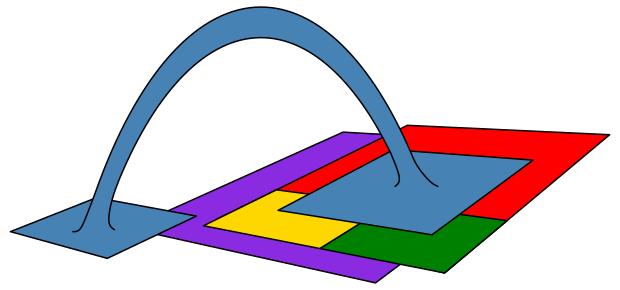
\includegraphics{bridge.png}
  \caption{A depiction of Peirce's Bridge for lines of identity}
  \footnotesize Source:\hspace{3pt}\url{https://commons.wikimedia.org/wiki/File:4CT_Inadequacy_Explanation.svg}
  \labfig{eg-bridge}
\end{marginfigure}

Thus he already identified the problem of readability stemming from having too
many lines or ``cables'' crossing eachother, a well-known concern in the design
of graphical programming languages\todo{Find reference}. This is to be opposed
to critics of the syntax of EG such as Quine, who invented a notation similar to
the lines of identity, and deemed it ``too cumbersome for practical
use''\todo{Find reference}. Also, the other proposed solution of having
so-called \emph{Bridges} is quite interesting, in that it makes the syntax of EG
\emph{three-dimensional}, in order to preserve the continuity of lines. A nice
illustration of the bridge is given in \reffig{eg-bridge}\sidenote{We found this
picture in the Wikipedia article on the \emph{four color theorem}
\cite{noauthor_four_2023}, which is no coincidence: according to Burch
\cite{sep-peirce}, \textit{``Peirce began to research the four-color map
conjecture, to work on the graphical mathematics of de Morgan's associate A. B.
Kempe, and to develop extensive connections between logic, algebra, and
topology, especially topological graph theory. Ultimately these researches bore
fruit in his existential graphs [...]''}. The Wikipedia article on Alfred Kempe
also mentions the following, to be connected with our multiset formalization of
EG \cite{noauthor_alfred_2023}: \textit{``Kempe (1886) revealed a rather marked
philosophical bent, and much influenced Charles Sanders Peirce. Kempe also
discovered what are now called multisets, although this fact was not noted until
long after his death.''}}.

\todo{ Use the following citation to explain how lines of identity are to be
  interpreted as quantifiers, where the term ``endoporeutic'', etymologically
  meaning ``from the outside to the inside'', refers to the relevance of the
  \emph{order} among quantifiers as to their meaning. }
  (\cite{peirce_prolegomena_1906}, p. 531):

\begin{quote}
  In the interpretation of Selectives it is often necessary to observe the rule
which holds throughout the System, that the Interpretation of Existential Graphs
must be \emph{endoporeutic}, that is, the application of a Graph on the Area of
a Cut will depend on the predetermination of the application of that which is on
the Place of the Cut.
\end{quote}
% % !TEX root =index.tex
\setchapterpreamble[u]{\margintoc}
\chapter{Asymmetric Bubble Calculus}
\labch{bubbles}

\epigraph{Leibniz sought to make the form of a symbol reflect its content. ``In
signs,'' he wrote, ``one sees an advantage for discovery that is greatest when
they express the exact nature of a thing briefly and, as it were, picture it;
then, indeed, the labor of thought is wonderfully diminished.''}
{\textbf{Frederick Kreiling}, \textit{Leibniz}, Scientific American, May 1968}


We introduce a new kind of \kl{nested sequent} \kl{proof system} dubbed \intro{bubble
calculus}. Inspired by the \emph{membrane} mechanism of the \intro{chemical
abstract machine} (\reintro{\cham}) \sidecite[25em]{berry_chemical_1989},
so-called \intro{bubbles} internalize the notion of \kl{subgoal} inside
\kl{sequents}, rather than through the tree structure induced by traditional
\kl{inference rules}. This allows for a more hierarchical representation of the
\kl{proof state}, where \kl(sequent){contexts} can be shared between different
\kl{subgoals}. In addition to the usual textual syntax, the \kl{bubble calculus}
can be expressed in a graphical syntax, where logical meaning is captured by
\emph{physical} constraints on \kl{diagrammatic} manipulations, instead of
\emph{virtual} restrictions on available \kl{inference rules}.

% We introduce a new kind of nested sequent \kl{proof systems} dubbed \emph{bubble
% calculi}. Inspired by the \emph{membrane} mechanism of the chemical abstract
% machine ({\cham} hereafter) \sidecite[25em]{berry_chemical_1989}, so-called
% \emph{bubbles} internalize the notion of \emph{subgoal} inside sequents, rather
% than through the tree structure induced by \kl{inference rules}. This allows for a
% more hierarchical representation of the proof state, where contexts can be
% shared between different subgoals. In addition to the usual textual syntax,
% bubble calculi can be expressed in a graphical syntax, where logical meaning is
% captured by \emph{physical} constraints on diagrammatic manipulations, instead
% of \emph{virtual} restrictions on available \kl{inference rules}. In the chemical
% metaphor, \emph{intuitionism} is then characterized as the phenomenon of
% \emph{repulsion} between objects that have the same polarity.

We start in \refsec{chemical} with the genesis of the idea of \kl{bubble calculus},
coming from the observation that our \kl{Proof-by-Action} paradigm (\refch{pba})
lends itself quite naturally to a \kl{metaphorical} interpretation, where actions are
seen as \emph{chemical} reactions. In \refsec{bubbles} we introduce the concept
of \emph{bubble} as a way to control the scope of hypotheses inside \kl{nested
sequents} that we call \emph{solutions}. In \refsec{asymmetric} we describe our
\kl{proof system} for \kl{intuitionistic} logic dubbed \emph{asymmetric \kl{bubble calculus}},
based on multiset \kl{rewriting rules} over solutions comprising at most one
conclusion. Finally in \refsec{bubbles-pba}, we import ideas from this \kl{bubble
calculus} back to the realm of \kl{GUIs} for interactive proof building, analysing
their possible impact for \kl{UX} improvements.


\section{The chemical metaphor}\labsec{chemical}

The \kl{Proof-by-Action} paradigm introduced in \refch{pba} offers multiple ways to
the user to attack the proof of a theorem: \kl{DnD} actions for \kl{subformula linking}
and equality rewriting are the main mechanism, but they only work in a goal
comprising multiple items. Since it is customary in \kl{proof assistants} to specify
the \kl{goal} to be proved as a single logical formula, one needs a way to decompose
it into many items for further processing through \kl{DnD}. This is precisely what
the \kl{introduction rules} for logical connectives in \kl{sequent calculus} do, and
following the \kl{Proof-by-Pointing} paradigm \cite{PbP} we map them to click
actions (see \refsec{clicks}).

So visually, a proof in \kl{Actema} consists in breaking logical items into subitems
positioned freely in space, and then bringing those subitems together to make
them interact and produce a new item. This is quite evocative of a
\emph{chemical reaction} controlled by the user, where logical formulas are akin
to molecules made of propositional atoms linked together by logical
connectives\sidenote{This precise \kl{metaphor} about the molecular structure of
propositions can already be found in Russell's introduction to Wittgenstein's
Tractatus Logico-Philosophicus, which was the main inspiration to his philosophy
of \emph{logical atomism} \cite[p.~11]{tractatus,klement_russells_2020}. Even
earlier in the history of logic, C. S. Peirce took inspiration from chemical
\kl{diagrams} to devise his \emph{existential graphs} --- see
\cite[pp.~17--18]{Roberts+1973}, or our own presentation in \refsec{beta} for
more details.}. Click actions are then a mean to ``heat'' molecules to the point
of breaking these chemical bonds. The most canonical examples are the \kl{right
introduction rule} for implication $\limp$ and the \kl{left introduction rule}
for conjunction $\land$, which break respectively a conclusion/red item/positive
ion into a hypothesis/blue item/negative ion and a new conclusion, and a
hypothesis into two hypotheses. In fact, it is strongly conjectured that these
are the only click actions needed to obtain a complete deductive system for
propositional logic: breaking red implications allows for \kl(dnd){backward}
\kl{DnDs}, and blue conjunctions for \kl(dnd){forward} \kl{DnDs}\sidenote{In
\kl{predicate logic}, one would also need the \kl[right introduction
rule]{right} (resp. \kl[left introduction rule]{left}) introduction rule for
$\forall$ (resp. $\exists$). It might also be the case that \kl(dnd){backward}
\kl{DnDs} alone are sufficient for completeness, since a \kl{linkage} of the
form $A \back \select{B} \limp C$ will involve a \kl(dnd){forward} phase. In
this case only the \kl{right introduction rules} for $\limp$ and $\forall$ would
be required.}.
% \sidenote{Interestingly,
% those rules are the basis for the adjunction between $\land$ and $\limp$ in the
% interpretation of IPL into cartesian closed categories.}

Rather than completeness, the issue here is \emph{consistency} of the user
interface: if the user is allowed to decompose red $\limp$ and blue $\land$, she
will assume naturally that she can also decompose blue $\limp$ and red $\land$,
as well as $\lor$ of any color. While red $\lor$ can be handled by pointing
directly at the disjunct to be proved, other configurations correspond to rules
of \kl{sequent calculus} with multiple premisses. In \kl{Actema}, this corresponds to
creating a new \kl{subgoal} for each premise, where \kl{subgoals} are displayed one at a
time in different \emph{tabs}: this new interface mechanism breaks the chemical
\kl{metaphor}. The root cause lies in the way \kl{sequent calculus} implements
\emph{context-scoping}: each \kl{subgoal} will share the same initial context of
hypotheses, but future hypotheses ``buried'' in the conclusions must be
available only in their respective \kl{subgoals}. The tabs mechanism implements this
by forcing the user to focus on exactly one tab/\kl{subgoal}, thus making it
impossible to display items from different \kl{subgoals} on the same screen, which
renders interaction between them physically impossible.


\section{Bubbles and solutions}\labsec{bubbles}

In order to accomodate context-scoping within the chemical \kl{metaphor}, we were led
to explore a notion of \emph{bubble} inspired by the \emph{membranes} of the
{\cham} \sidecite{berry_chemical_1989}. The latter are used to delineate zones
of \emph{local} interaction, which are still porous to external data. This is
precisely what we want to do here: let us consider that the user tries to prove
the \kl{sequent} $\Gamma \seq A \land B$. By clicking on the red item $A \land B$,
she will break it into two \kl{bubbles} $\bubbleT{\seq A}$ and $\bubbleT{\seq B}$.
Then she might decompose $A$ and $B$ further into \kl{sequents} $\sigma_A = \Gamma_A
\seq C_A$ and $\sigma_B = \Gamma_B \seq C_B$, and use hypotheses from $\Gamma$
by dragging them inside either $\bubbleT{\sigma_A}$ or $\bubbleT{\sigma_B}$.
However, hypotheses from $\Gamma_A$ and $\Gamma_B$ cannot be dragged out from
their respective bubble, since then they could be used in the other \kl{bubble} and
violate context-scoping.

This situation is illustrated in \reffig{bubbles-flow}, where \kl{bubbles} are
represented by gray circles, and possible drag moves of formulas by arrows. More
specifically, green and orange arrows \kl{symbolize} respectively valid and invalid
moves. Notice how this graphical depiction of \kl{bubbles} exhibits their
\emph{topological} behavior: while objects can enter inside \kl{bubbles} from the
outside, they get blocked by the membrane in the opposite direction. Indeed the
only relevant feature of the circle representation is that it divides the space
into an \emph{interior} and an \emph{exterior}. Then the \emph{nesting} of
circles and the \emph{positions} of formulas relative to them encode
respectively the \emph{tree} structure of the proof, and the scope of hypotheses
in it.

\begin{figure}
\stkfig{1.5}{bubbles-flow}
\caption{Context-scoping in \kl{bubbles} as topological constraints}
\labfig{bubbles-flow}
\end{figure}
\kl{Bubbles} can also be seen as a way to internalize in the syntax of \kl{sequents} the
notion of \emph{subgoal}, which requires in turn to allow nesting of \kl{sequents}
inside each other. The \kl{proof state} is not a set of \kl{subgoals} anymore, but a
single \kl{nested sequent} of this sort, that we call a \emph{solution}\sidenote{The
term ``solution'' refers here to the \kl{metaphor} of a \emph{chemical solution} made
up of an unordered collection of molecules. Which is quite ironic, since we use
it to denote \kl{goals} waiting to be proved, that is problems lacking a
solution\dots}. In textual syntax, solutions $S$ are generated by the
following grammar:
\begin{mathpar}
S, T, U \Coloneq \Gamma \piq{S_1 \sep \ldots \sep S_n} \Delta
\and
\Gamma, \Delta \Coloneq A_1, \ldots, A_n
\end{mathpar}
where the $A_i$ are usual formulas of \kl{FOL}. Thus solutions are just like
sequents, except that we add a collection of nested solutions $S_i$ that will
represent \kl{subgoals}, or premisses of usual \kl{inference rules}. To be more precise,
the collections of formulas $A_i$ and solutions $S_i$ are \emph{multisets},
which gives the following mutually recursive definitions:
\begin{definition}[Ion]
An \emph{ion} is a formula charged either \emph{negatively} (hypothesis) or
\emph{positively} (conclusion).
\end{definition}
\begin{definition}[Bubble]
A \emph{bubble} is a solution enclosed in a membrane.
\end{definition}
\begin{definition}[Solution]\labdef{solution}
A \emph{solution} $S$ is a multiset of ions and bubbles. It is
\emph{single-conclusion} if it contains at most one positive ion. We will use
letters $\cS, \mathcal{T}, \mathcal{U}$ to denote multisets of
solutions.
\end{definition}
Note that in the above definitions, \kl{bubbles} play a purely \kl{metaphorical} role and
could be dispensed with. But it will be useful later on to distinguish them
conceptually from solutions.

\section{Asymmetric calculus}\labsec{asymmetric}

\subsection{Interpreting solutions}

A natural way to give logical meaning to a solution is to translate it into a
formula. In the following we provide one such translation, which will play a
determining role in the design of \kl{inference rules} for manipulating solutions. We
qualify it of \emph{asymmetric} because it only works for single-conclusion
solutions, in the same way that \kl{LJ} only works for single-conclusion
sequents.

\begin{remark}
In this section we only deal with single-conclusion solutions, but the more
general case will be studied starting from \refsec{branching}.
\end{remark}

Just like a sequent, a solution is semantically equivalent to an implication,
except that we add the \emph{conjunction} of all \kl{subgoals} to the consequent:

\begin{definition}[Asymmetric interpretation]\labdef{ainterp}
The \emph{asymmetric interpretation} of a solution is defined recursively by:
$$\aint{\Gamma \piq{S_1 \sep \ldots \sep S_n} \Delta} = \bigwedge \Gamma
  \limp \bigwedge \Delta \land \bigwedge_i{\aint{S_i}}$$
\end{definition}

Note that we join formulas in $\Delta$ conjunctively: since we do not consider
solutions with more than one conclusion, this is just to handle the case where
$\Delta = \emptyset$, and thus $\bigwedge \Delta = \top$. This subtle detail is
in fact essential to the way we encode the tree structure of proofs inside
solutions:
\begin{itemize}
\item a solution with one conclusion corresponds to a \emph{leaf} of the proof
tree, i.e. a \kl{subgoal};
\item a solution with no conclusion corresponds to a \emph{node} of the proof
tree, i.e. a branching point where we created multiple \kl{subgoals}.
\end{itemize}
This will soon become clearer with examples of derivations in our calculus. In
\refsec{branching}, we will consider a different interpretation of solutions that
entails a different encoding of the proof structure in them.

\subsection{Sequent-style rules}

\begin{figure*}
\input{figures/sequent-BJ.tex}
\caption{Sequent-style presentation of the asymmetric \kl{bubble calculus} \kl{BJ}}
\labfig{sequent-BJ}
\end{figure*}

Our initial idea for a \kl{proof system} based on solutions was quite simple: we take
the \kl{inference rules} of \kl{LJ}, and turn them all into unary rules by encoding
premisses as bubbles. This gives the basis for the set of rules presented in
\reffig{sequent-BJ}, that defines our asymmetric \kl{bubble
calculus} for \kl{intuitionistic} logic dubbed \kl{BJ}. It is divided in five groups:
\begin{itemize}
\item The {\identity}, {\resource} and {\heating} groups correspond
respectively to the identity, structural and logical rules of \kl{sequent
calculus}, following the terminology of \sidecite{girard:hal-01322183}. More
precisely, rules {\rsf{i{\da}}} and {\rsf{i{\ua}}} correspond
to the axiom and cut rules; rules {\rsf{w}} and {\rsf{c}} to the \kl{weakening}
and \kl{contraction} rules; and every rule of the form $\mcirc{-}$ (resp.) that
is, the axiom and cut rules, the \kl{contraction} and \kl{weakening} rules, and
\kl{introduction rules} for logical connectives.
\item The {\flow} and {\membrane} groups are new, and define the behavior of
bubbles. More specifically, $\mathbb{F}$-rules characterize how information
flows in solutions by specifying what kinds of objects can traverse bubbles,
and in which direction. They play the same role as \emph{switch} rules in
formalisms based on \kl{CoS} \cite{Guglielmi1999ACO}, which includes our own
\kl{subformula linking} rules (\reffig{DISL}). In the asymmetric \kl{bubble calculus}
there is only one $\mathbb{F}$-rule {\rsf{f{-}}} allowing hypotheses to flow
inside bubbles.

As their name suggests, $\mathbb{M}$-rules handle the behavior of the
\emph{membrane} of bubbles, but independently from other items as opposed to
$\mathbb{F}$-rules. In the asymmetric \kl{bubble calculus} there is only one
$\mathbb{M}$-rule {\rsf{p}} allowing to \emph{pop} any empty bubble, which
can be interpreted as the action of dismissing a solved \kl{subgoal}. In \kl{CoS} it
would correspond to congruence rules handling the truth unit $\top$, and in
\kl{subformula linking} to the unit rules (\reffig{DISL-U}).
\end{itemize}

Now that we have rules for manipulating solutions, and since solutions can be
nested through bubbles, we need a notion of \emph{context} for applying rules on
subsolutions of arbitrary depth:

\begin{definition}[Context]\labdef{solution-context}
% \emph{Solution contexts} are defined by the following grammar:
% $$S\hole \Coloneq \hole \mid \Gamma \piq{\cS \sep S\hole \sep
% \mathcal{T}} \Delta$$
A \intro{context} $S\hole$ is a solution which contains exactly one
occurrence of a special solution written $\hole$, called its \reintro{hole}.
Given another solution $T$, we write $S\select{T}$ to denote the solution equal
to $S\hole$ where $\hole$ has been replaced by $T$.
\end{definition}

Then every rule of \reffig{sequent-BJ} is applicable in any
\kl{context} $U\hole$. That is:
$$\vcenter{\R{S}{T}} \quad \text{should be read as} \quad
\vcenter{\R{U\select{S}}{U\select{T}}} \quad \text{for all $U\hole$}$$

\begin{definition}[\kl{BJ}-step]\labdef{BJ-step}
We write $S \lstep{} T$ to denote the existence of a \kl{BJ}-rule instance
$\irule{r}{S}{T}$ in the empty \kl{context}, i.e. $S$ and $T$ are respectively the
conclusion and premiss of the rule {\rsf{r}} in \reffig{sequent-BJ}, modulo
instantiation of meta-variables\sidenote[][-11cm]{The direction of the arrow
is from conclusion to premiss, to stay consistent with our interactive proof
building setting where \kl{inference rules} are seen as \kl{goal}-modifying actions.}.
Then $\lstep{}$ can be seen as a binary relation on solutions, whose contextual
closure described above is the \emph{step} relation $\step{}$: $S \step{} T$ if
and only if there exist $U\hole$, $S_0$ and $T_0$ such that $S =
U\select{S_0}$, $T = U\select{T_0}$ and $S_0 \lstep{} T_0$.
\end{definition}

\begin{definition}[\kl{BJ}-derivation]\labdef{BJ-deriv}

A \emph{derivation} $\deriv{\mathcal{D}}{S}{T}$ in \kl{BJ} is a list
$\mathcal{D}$ of \kl{BJ}-steps with premiss $T$ and conclusion $S$.
\end{definition}

\begin{definition}[\kl{BJ}-proof]\labdef{BJ-proof}
A \emph{proof} of a solution $S$ in \kl{BJ} is a derivation
$\deriv{\mathcal{D}}{S}{\piq{}}$ that reduces $S$ to the empty solution, which
denotes the \kl{proof state} where there are no \kl{subgoals} left.
\end{definition}

\begin{marginfigure}
\input{figures/ex-seq-BJ.tex}
\caption{Example of sequent-style proof in \kl{BJ}}
\labfig{ex-seq-BJ}
\end{marginfigure}

\subsection{Proof-as-trace}

An example of proof in \kl{BJ} is shown in \reffig{ex-seq-BJ}, where the
focused subsolution is squared for each inference. Notice that many rules could
have been applied in a different order: for instance all applications of the
{\rsf{p}} rule could have been postponed to the top/end of the derivation.
This is generally true of all formalisms based on \kl{CoS}, which is known in the
\kl{deep inference} literature for its ``bureaucracy''. In \kl{BJ},
$\mathbb{H}$-rules aggravate the matter by adding all inessential rule
permutations from \kl{sequent calculus} to those of \kl{CoS}. As our wording suggests,
this is usually perceived negatively in \kl{deep inference} \kl{proof theory}, where a
central question is that of finding \emph{canonical} representations of proof
objects \sidecite{strasburger-problem-2019}.

However in our interactive proof-building setting, it should rather be seen as a
\emph{desirable} property of the system. Indeed, one consequence is that the
user has more freedom to organize her reasoning in whichever order she wants, in
an incremental and guided way. One should remember that in the \kl{Proof-by-Action}
paradigm, the focus is not the proof object, which is implicit and hidden to the
user, but the \emph{process} of building it. Then a \kl{BJ}-derivation is
better understood as the \emph{trace} of this building process, rather than the
constructed proof\sidenote{The idea of \emph{proof-as-trace} is relatively
common in logic programming \cite{miller_survey_2022}, but not so much in \kl{deep
inference} \kl{proof theory}. It is Jean-Baptiste Joinet who shared with us his idea
of applying it in this setting, based on his own work interpreting \kl{CoS} for
\kl{MLL} as a system for building \emph{multiplicative proof nets}
\cite{joinet_completeness_2007}.}. And the fact that this trace corresponds, or
can be transformed into a more canonical representation is of no concern to the
user. What matters for a good proof-building interface is to be as flexible as
possible, in order to match the user's own mental process of argumentation.

Of course flexibility comes at a price, and the rules of \kl{BJ} are probably
too numerous and low-level to be mapped directly into individual proof actions
in a user interface. Some of these concerns will be tackled in
\refsubsec{bubbles-search}, but we think a better answer might have been found
with the \kl{proof system} introduced in \refch{flowers}, and its associated
prototype of \kl{GUI} presented in \refsec{flowers-prover}.

\todo{ This section might be getting too long with too many subsections; will
  probably need to move philosophical reflections like this somewhere else.
  Maybe a conclusion to this chapter? But the ideas seem to apply to all systems
  in this thesis, and thus may deserve a more general rewording in
  \refch{intro}. }

\subsection{Graphical rules}\labsec{bubbles-graphical-rules}

\begin{figure*}
  \input{figures/graphical-BJ}
  \caption{Graphical presentation of the asymmetric \kl{bubble calculus} \kl{BJ}}
  \labfig{graphical-BJ}
\end{figure*}

While the sequent-style presentation of \kl{BJ} clearly shows its filiation
with \kl{sequent calculus}, its syntax is quite heavy, and obscures an important
property of the rules: they almost always preserve the \kl(sequent){contexts} $\Gamma, \Delta$
of formulas and $\cS$ of bubbles. That is, the rules of \kl{BJ} are
\emph{local}. This enables a more economical and graphical presentation of the
rules in \reffig{graphical-BJ}, where \kl{BJ} is seen as a multiset \kl{rewriting
system} just like the {\cham} thanks to \refdef{solution}. Instead of relying on
a notion of solution \kl{context}, we define formally what it means to be a
subsolution:

\begin{definition}[Subsolution]\labdef{subsolution}
  $S$ is a \emph{subsolution} of $T$, written $S \subsol T$, if either $S
  \subseteq T$ or $S \subsol T_0$ for some $T_0 \in T$, where $\subseteq$
  denotes multiset inclusion. 
\end{definition}

Then a multiset \kl{rewriting rule} $\rrule{r}{S}{T}$ can be applied in a
solution $U$ whenever $S \subsol U$, by replacing one occurrence of $S$ by $T$
inside $U$. The notions of derivation (\refdef{BJ-deriv}) and proof
(\refdef{BJ-proof}) stay unchanged, by observing that the \kl{rewriting rule}
$\rrule{r}{S}{T}$ from $S$ to $T$ and the \kl{inference rule}
$\irule{r}{S}{T}$ with premiss $T$ and conclusion $S$ denote the same
rule $r$.

\todo{Add definition of multiset inclusion somewhere?}

\todo{Maybe split both \reffig{ex-gra-BJ} and \reffig{ex-seq-BJ} in two figures,
one for the beginning of the proof upto {\rsf{f{-}}}, and a generic one for
the two subproofs starting with {\rsf{{\limp}{-}}}.}

\reffig{ex-gra-BJ} shows the graphical presentation of the same \kl{BJ}-proof
as in \reffig{ex-seq-BJ}. Whereas in \reffig{ex-seq-BJ} we squared the whole
subsolutions corresponding to the conclusions of \kl{inference rules}, here we
squared on each line the redex modified by the associated \kl{rewriting rule}. This
example highlights the greater locality of the rewriting approach, by indicating
more precisely which parts of the \kl{proof state} are changed by the rules. But it
still over-approximates the modifications that really need to be performed to
carry the transformations. Indeed, by only exposing the data of a redex $S$ and
a reddendum $T$, a \kl{rewriting rule} $\rrule{r}{S}{T}$ can only be
interpreted as the deletion of $S$ followed by the insertion $T$. Taking for
instance the {\rsf{{\limp}{-}}} rule in \reffig{graphical-BJ}, one can
describe its graphical behavior more finely as resulting from the following
sequence of \emph{edits}:
\begin{enumerate}
  \item Erase the $\hypo{{\limp}}$ connective;
  \item Change the polarity of $\hypo{A}$ from hypothesis to conclusion;
  \item Insert a new empty bubble;
  \item Move $\conc{A}$ in this bubble;
  \item Insert a new empty bubble;
  \item Move $\hypo{B}$ in this bubble;
  \item If $\conc{\Delta}$ is not empty, also move $\conc{\Delta}$ in this bubble.
\end{enumerate}
It would be interesting to consider the question of finding a minimal set of
edit operations like these, that can simulate all the rules of
\kl{BJ}\sidenote{As will become apparent in \refsec{bubbles-completeness},
\kl{BJ} itself provides a finer-grained simulation of the rules of \kl{sequent
calculus}, which in turn is known to be a more detailed variant of
\emph{\kl{natural deduction}}. Interestingly through the \kl{Curry-Howard
isomorphism}, this would correspond to a \emph{chain of compilation}, starting
from the higher-level \kl{$\lambda$-calculus} (\kl{natural deduction}), going into
abstract machines (\kl{sequent calculus}) \cite{downen_sequent_2016}, down to
something akin to \emph{assembly language} with \texttt{jump} instructions
(Section 6.3.1 of \cite{guenot_nested_2013}).}. Note however that most of the
above edits are \emph{unsound} as reasoning steps. If not for logical insight,
such an edit calculus could still be relevant \emph{computationally}, typically
by enabling efficient implementations of the rules with a small memory
footprint.

\begin{figure*}
  \input{figures/ex-gra-BJ.tex}
  \caption{Example of graphical proof in \kl{BJ}}
  \labfig{ex-gra-BJ}
\end{figure*}

\section{Back to Proof-by-Action}\labsec{bubbles-pba}

When looking at the \kl{BJ}-proof of \reffig{ex-gra-BJ}, the astute reader
might have been reminded of the \kl{Proof-by-Action} paradigm as introduced in
\refch{pba}, by seeing redexes as the items involved in a graphical action ---
there are always at most two. More precisely, $\mathbb{H}$-rules correspond to
\emph{click} actions on blue ({\rnm{\mcirc{-}}} rules) or red items
({\rnm{\mcirc{+}}} rules), and the {\rsf{i{\da}}} rule corresponds to
the most basic \kl{DnD} action between dual occurrences of a formula.

As mentioned earlier when comparing \kl{BJ} to \sys{LJ}, the novelty here lies
with $\mathbb{H}$-rules, $\mathbb{F}$-rules and $\mathbb{M}$-rules that deal
with \emph{bubbles}. Remember that the goal behind the idea of \kl{bubble calculus}
was precisely to provide a new way to manipulate \kl{subgoals} through \kl{bubbles}
instead of tabs, which are more in line with the chemical \kl{metaphor}. It is quite
easy to imagine a \kl{GUI} presenting the \kl{proof state} as a solution, in a graphical
layout close to that of \reffig{ex-gra-BJ}\sidenote{Although there might be some
challenges in implementing an efficient layouting algorithm for bubbles,
typically to make solutions fit into the screen.}. Like formulas in blue and red
items, whole \kl{subgoals} could now be shown on the same screen in their respective
bubbles, and be freely moved around with a pointing device. Following are some
ideas for mapping the remaining rules of \kl{BJ} in such a \kl{GUI}:

\begin{marginfigure}
  $$
  \begin{array}{rcll}
    \hypo{A}~~~\hypo{B} &\step{} &\hypo{A \forw B} &\forw \\
    \hypo{A}~~~\conc{B} &\step{} &\conc{A \back B} &\back \\
  \end{array}
  $$
  \caption{\kl{Linkage} creation rules in \kl{BJ}}
  \labfig{bubbles-linkage}
\end{marginfigure}

% \begin{marginfigure}
%   $$
%   \begin{array}{rcll}
%     \conc{t = t} &\step{} &&{=}{+} \\
%     \hypo{t = u}~~~A &\step{} &\subst{A}{u}{t} &{=}{-}1 \\
%     \hypo{t = u}~~~A &\step{} &\subst{A}{t}{u} &{=}{-}2 \\
%   \end{array}
%   $$
%   \caption{Rules for equality in \kl{BJ}}
%   \labfig{bubbles-eq}
% \end{marginfigure}

% \begin{marginfigure}
%   \input{figures/bubbles-vars.tex}
%   \caption{Rules for variables and definitions in \kl{BJ}}
%   \labfig{bubbles-vars}
% \end{marginfigure}

\begin{description}
  \item[\textbf{\flow}]
    The {\rsf{f{-}}} rule plays a special role, in that it would not be mapped
    to any particular action. Indeed it captures the way information flows in
    solutions, and we already described in \refsec{bubbles} how this is
    reflected in the topological behavior of bubbles. Thus it could be
    implemented in the graphical interface as a kind of \emph{physics engine}:
    when dragging an item around the proof canvas, it would get stuck on the
    membrane of bubbles, except if it is blue and the drag movement goes inward.
    This of course would provide a level of interactivity unseen before in a
    proving interface, making it very discoverable and playful. It also combines
    nicely with \kl{DnD} actions in general: for instance a sequence of applications
    of {\rsf{f{-}}} followed by {\rsf{i{\da}}} could be performed as
    a single \kl{DnD} action, where the dragged hypothesis crosses successively the
    various \kl{bubbles} in its way.
  \item[\textbf{\membrane}]
    The {\rsf{p}} rule can be mapped very straightforwardly to the action of
    clicking on the area of an empty bubble, in order to pop it. It could also
    be entirely automated, by letting the proof engine eagerly pop empty \kl{bubbles} as soon as they appear in a solution. Note that in this graphical setting,
    the {\rsf{p}} rule can be understood as resulting from a process of
    \emph{contraction}\sidenote{Not to be confused with the \kl{contraction} rule
    \rsf{c}.} of the membrane into a single point: if the \kl{bubble} contains some
    items $\Delta$, then this process fails because the membrane gets stuck on
    the boundaries of $\Delta$. This is a topological way to check the emptiness
    of a bubble, which has the benefit of being completely \emph{local}, on top
    of being very clear visually.
  \item[\textbf{\resource}]
    % In Actema, hypotheses are displayed in blue items inside a reserved zone
    % holding the entire context, including also local variables and definitions
    % in green items. The resource behavior of blue items placed by the user in
    % the proof canvas differs from those in the context zone: while the former
    % are consumed after a backward or forward \kl{DnD}, the latter are preserved and
    % thus implicitly duplicated\sidenote{In the literature on focusing in linear
    % logic, this corresponds roughly to the distinction between the \emph{storage
    % zone} in sequents where formulas can be duplicated and discarded at will,
    % and the \emph{linear zone} where they cannot.}. In a bubble-based \kl{GUI}, one
    % could keep this behavior, where the context is filled with all items 
    The \kl{contraction} rule {\rsf{c}} could be mapped to a specific triggering
    input when starting to drag a blue item $\hypo{A}$ (e.g. a shortkey if a
    keyboard is available, or a long press on the item on a touchscreen), which
    has the effect of keeping a copy of $A$ at its original location in addition
    to moving the item\sidenote{This mechanism is quite standard in \kl{GUIs} that
    manipulate duplicable resources like file managers, where one maintains the
    \texttt{CTRL} key to enable copy mode. It was also chosen by K. Chaudhuri to
    implement \kl{contraction} in his \kl{ProfInt} prototype for \kl{subformula linking}
    in \kl{intuitionistic} logic \cite{ProfInt}.}. As for the \kl{weakening} rule
    {\rsf{w}}, it could be available as a contextual action when selecting
    blue items.
  \item[\textbf{\identity}]
    Although the {\rsf{i{\da}}} rule only corresponds to the base case
    of \kl{DnD} actions, it would be easy to integrate their full SFL semantics
    directly in \kl{BJ}. Indeed our SFL rules (\reffig{DISL}) are already
    expressed as \kl{rewriting rules}, just like the graphical rules of \kl{BJ}
    (\reffig{graphical-BJ}). Thus it is just a matter of adding \kl{linkage} creation
    rules like those of \refsec{dnd-completeness}, but between adjacent formulas
    in a solution (see \reffig{bubbles-linkage}).

    The cut rule was handled in \kl{Actema} with a separate \textsf{+hyp}
    button, which adds the cut formula $A$ (input by the user in a dialog box)
    as a new hypothesis in the current \kl{goal}, and as the conclusion in a new
    \kl{subgoal} (see \refsubsec{pba-layout}). Since \kl{subgoals} are now reified as
    bubbles, the {\rsf{i{\ua}}} rule could be mapped instead to a contextual
    action available on any red item $\conc{\Delta}$, which would have the
    effect of spawning a \kl{bubble} around it with a blue item $\hypo{A}$, and
    another \kl{bubble} nearby it with a red item $\conc{A}$.

    % Finally, an analog to the cut rule {\rsf{i{\ua}}} is the rule
    % {\rsf{d\ua}} for adding new definitions (\reffig{bubbles-vars}).
    % Their similarity is more striking in a logical framework like Martin-Löf
    % type theory, where mathematical objects and propositions are expressed in
    % the same language. In Actema it is handled with a separate \textsf{+expr}
    % button, and could here be mapped to a contextual action available anywhere
    % on the proof canvas\sidenote{In type theory, the body of type $T$ of the
    % definition could be left for completion as a new subgoal with conclusion
    % $T$, and thus be expressed as a new bubble that can be solved later.}.
  \item[\textbf{\heating}]
    For $\mathbb{H}$-rules that spawn \kl{bubbles} like {\rnm{\land{+}}}, it is
    important that \kl{bubbles} stay close to the item being clicked, in order to
    make the transformation clear visually. One could even imagine a small
    animation that smoothly turns the main connective into bubbles, to convey
    more effectively the intuition that heating rules break logical connectives
    seen as chemical bonds.

    % Regarding the rules involving quantifiers, two remarks are in order:
    % \begin{itemize}
    %   \item In Actema, rules {\rnm{\forall{+}}} and {\rnm{\exists{-}}} would
    %   introduce a new green variable in the context. To accomodate for this in a
    %   bubble-based \kl{GUI}, one needs to extend the notion of solution so that
    %   it incorporates local variables, in addition to formulas:
    %   \begin{align*}
    %     \Gamma, \Delta &\Coloneq \iota_1, \ldots, \iota_n \\
    %     % \iota &\Coloneq A \mid \delta \\
    %     % \delta &\Coloneq x \mid \ldef{x}{t}
    %     \iota &\Coloneq A \mid \ldef{x}{\beta} \\
    %     \beta &\Coloneq \emptyset \mid t
    %   \end{align*}
    %   In this syntax, $\ldef{x}{t}$ represents a local definition with name $x$
    %   and body $t$, and $\ldef{x}{\emptyset}$ a local variable with name $x$.
    %   That is, variables are seen as definitions without a body. Then rules
    %   {\rnm{\forall{+}}} and {\rnm{\exists{-}}} are modified accordingly (see
    %   \reffig{bubbles-vars}).
    %   \item Instantiation rules {\rnm{\forall{-}}} and {\rnm{\exists{+}}} could
    %   be mapped as in Actema to \kl{DnD} actions with a green item, corresponding to
    %   the alternative formulation of \reffig{bubbles-vars}. This way all the
    %   rules of \kl{BJ} become \emph{analytic}: if $S \step{} T$, then every
    %   subterm occurring in $T$ also occurs in $S$\sidenote{The only exceptions
    %   are the {\rsf{i{\da}}} rule which will be shown to be admissible
    %   in \refsec{bubbles-completeness}, and the {\rsf{d{\ua}}} rule of
    %   \reffig{bubbles-vars}.}.
    % \end{itemize}
\end{description}

Beyond the recovered uniformity of the user interface in terms of the chemical
\kl{metaphor}, \kl{BJ} exhibits some features that are interesting both at the
\kl{proof-theoretical} and user-experience levels:
\begin{description}
  \item[\textbf{Factorization}] It implements a form of \emph{context-sharing}
    between \kl{subgoals}: that is, one can perform transformations on shared
    hypotheses (\kl{forward} reasoning) without going back to a \kl{proof state} anterior
    to the splitting of said \kl{subgoals}. This should simplify the navigation in
    the proof as it is being constructed, by avoiding the need to locate these
    splitting points. In fact often beginners (but also occasionally seasoned
    users) do not have the reflex to do this, precisely because the interface
    makes it difficult. This results in proofs with a lot of duplicated
    arguments, since splitting \kl{goals} systematically duplicates the \kl(sequent){context} of
    hypotheses. Thus \kl{bubbles} can be seen as a mechanism that favors by default a
    style of proof with better factorization of
    subproofs.\label{par:factorization}

  \item[\textbf{Navigation}] The tree structure of \kl{subgoals} is immediately
    apparent in the \kl{proof state} through the nesting of bubbles. Thus part of the
    information on the proof construction process, which was made implicit and
    temporal in the \kl{proof state} history, is now made explicit and spatial in the
    \kl{proof state} itself\sidenote{This concern of finding an explicit graphical
    representation of the ``motions of reasoning \emph{in actu}'', and not only
    the states of mind, can be found already in the works of Peirce on his
    existential graphs \cite[pp.~112--113]{Roberts+1973}. We will come back to
    this in \refch{eg}.}.
    
    There are multiple ways to visualize trees on a planar surface, but if we
    are to maintain the \kl{bubble} \kl{metaphor}, \emph{zoomable user interfaces} seem to
    be a right fit: they allow for efficient space management and navigation,
    and zooming in intuitively conveys the idea of focusing on a specific
    \kl{subgoal}. One could also zoom out to have an overview of the different
    \kl{subgoals} and their shared \kl(sequent){context}, something which is hard to do in current
    \kl{proof assistants}.
    
    When zoomed in on a \kl{subgoal}, the shared \kl(sequent){contexts} around it will not be
    visible anymore. While this is useful to focus attention and avoid being
    distracted by other \kl{subgoals}, it can quickly become cumbersome for the user
    to always have to zoom out in order to retrieve hypotheses from these shared
    \kl(sequent){contexts}. One solution would be to rebrand the \kl(sequent){context} zone of \kl{Actema} as a
    \emph{global} \kl(sequent){context} zone, where all the shared \kl(sequent){contexts} available in the
    \kl{subgoal} under focus are merged in a single list, and immediately accessible
    for manipulation. Of course actions performed in the \kl(sequent){context} zone would be
    reflected in the proof canvas, and vice versa.

  \item[\textbf{Goal diffing}] From a user perspective, the locality of rules
    means that applying some action to one or two items will not involve other
    items\sidenote{The only exceptions are clicks on blue $\bot$, $\lor$ and
    ${\limp}$, but the only extra item they involve is the conclusion.}.
    Non-local rules are less natural for a beginner because they modify a global
    state (here other items and \kl{subgoals}) which is not clearly correlated to the
    transformed data, often because it is not immediately visible.

    For instance in \kl{Actema}, many users have reported difficulties in
    understanding the effect of click actions that create new \kl{subgoals}. A first
    reason that can easily be remedied, is that there was not enough visual
    feedback to indicate the newly created tabs. But a deeper limitation is that
    the user needs to explicitly focus on these \kl{subgoals} to show their content,
    which they might not do immediately. And then it gets difficult to keep
    track of the origin of said \kl{subgoals} without a way to visualize the tree
    structure of the proof.

    All these concerns can be addressed within the \kl{bubble} \kl{metaphor}: since \kl{bubbles} are items freely positioned on the canvas, all the new items
    produced by an action can stay near the location where the action was
    initiated (i.e. the click or drop location); and since all transformations
    are local, all items not involved in the action can have their locations
    preserved. In other words, \kl{bubbles} make it easier to understand the
    \emph{difference} between a \kl{goal} and \kl{subgoals} generated by a proof action,
    which is crucial when learning the semantics of actions through practice.
    % This is of limited importance however in our case, because \kl{sequent calculus}
    % rules always perform the same trivial operation on the global state:
    % duplicating the whole context of hypotheses.
\end{description}

% \setchapterpreamble[u]{\margintoc}
\chapter{Existential Graphs}
\labch{eg}

\todo{Add citation from Peirce}

C. S. Peirce is famous for his contributions to symbolic logic, including among
others his eponymous law for classical logic, and his pioneering work on the
algebra of relations and quantification \cite{peirce_algebra_1885}. But far less
widespread are his achievements in the realm of graphical logic, or \emph{iconic
logic} as Shin calls it \cite{10.7551/mitpress/3633.001.0001}. He dedicated a
large chunk of his life investigating diagrammatic systems, starting in 1882
with the \emph{entitative graphs} and culminating with the \emph{existential
graphs}, which he developed from 1896 until his death in 1914
\cite{Roberts+1973}. Interestingly, Peirce perceived existential graphs
(thereafter ``EG'') as his \textit{``chef d'oeuvre''}, and that they
\textit{``ought to be the logic of the future''}\sidenote[][3em]{Both citations
are sourced in page 11 of \cite{Roberts+1973}.}.

\begin{tikzpicture}
  \directlua{
    dofile("../flower.lua").one({
      petals = {
        {name="Alpha", color="blue"},
        {},
        {}
      }
    })
  }
\end{tikzpicture}

Recent works have started to realize this vision: for example Sowa based his
conceptual graphs for computerized knowledge representation on EG
\cite{sowa_conceptual_1976}, Brady, Trimble
\cite{brady_categorical_2000}\cite{brady_string_nodate} and Haydon, Sobociński
\cite{pietarinen_compositional_2020} proposed various reconstructions of EG
through the lens of \emph{topology} and \emph{category theory}, and Melliès and
Zeilberger \cite{mellies_bifibrational_2016} refined the interpretation of Brady
and Trimble by making further connections with \emph{linear logic}
\cite{girard-linear-1987}. The full story has yet to be told, but we hope that
our work will constitute one more step towards the vision Peirce had in mind.

In this chapter, we propose a self-contained exposition of EG, that tries at the
same time to be faithful to the original presentation of the systems by Peirce,
and more modern in some aspects of their formalization. The goal will be to
familiarize the reader with the unique approach to proofs inherent to EG, which
can be difficult to relate to more standard frameworks like Hilbert and Gentzen
proof systems, and even deep inference proof systems like the calculus of
structures. This shall prove useful to get a good understanding of the
historical and technical foundations behind our \emph{flower calculus}, to be
introduced in \refch{flowers}.

The chapter is organized as follows: we start in \refsec{alpha} by presenting
the diagrammatic syntax of the system \sys{Alpha} of EG for classical
propositional logic. In \refsec{illative}, we introduce the inference rules of
\sys{Alpha} for manipulating existential graphs, called \emph{illative
transformations} by Peirce. In \refsec{multisets}, we give an equivalent
formulation of the syntax and rules of \sys{Alpha} as a \emph{multiset}
rewriting system. In \refsec{atomicity}, we formalize a variant of the
(de)iteration principle described by Peirce in
\sidecite{peirce_prolegomena_1906} that eliminates the need for the double-cut
principle, and discuss how it was motivated by Peirce's quest for \emph{illative
atomicity}. In \refsec{eg-soundness}, we take advantage of our reformulation to
give a simple proof of soundness for \sys{Alpha}, based on a direct
truth-evaluation of graphs. In \refsec{eg-completeness} we give a novel
syntactic proof of completeness for \sys{Alpha}, by simulating the calculus of
structures \sys{SKS} of Brünnler and Tiu \cite{brunnler_local_2001}. In this
way, \sys{Alpha} is shown to have subsystems that inherit the \emph{locality}
property of \sys{SKS}, and where the deletion and insertion rules are
respectively admissible for \emph{provability} and \emph{refutability}, making
\sys{Alpha} \emph{analytic}. In \refsec{beta}, we illustrate the original
mechanism of \emph{lines of identity} used by Peirce to handle quantifiers and
equality in his \sys{Beta} system. We end in \refsec{gardens} by showing how to
recast lines of identity in a more traditional binder-based syntax.

% \todo{IDEA (where should we put it?): \emph{superposition of polarities} in
% existential graphs. While a cut in bubble calculi is the insertion of \emph{two}
% occurrences of the same formula with \emph{distinct} polarities, the insertion
% rule only introduces \emph{one} occurrence of the formula, which plays either a
% negative role when it is iterated, or a positive role when it is deiterated}


\section{\sys{Alpha} graphs}\labsec{alpha}

Peirce designed in total three systems of EG, which he called respectively
\sys{Alpha}, \sys{Beta} and \sys{Gamma}. They were invented chronologically in
that order, which also captures their relationship in terms of complexity:
\sys{Alpha} is the foundation on which the other systems are built, and can
today be understood as a diagrammatic calculus for classical
\emph{propositional} logic. As we will see in \refsec{Quantification},
\sys{Beta} corresponds to a variable-free representation of \emph{predicate}
logic without function symbols, and with primitive support for \emph{equality}.
The last system \sys{Gamma} is more experimental, with various unfinished
features that have been interpreted as attempts to capture \emph{modal}
\sidecite{zeman_graphical_1964} and \emph{higher-order} logics\sidenote{A less
known fact is that at the end of his life, Peirce pushed his experimentations
beyond the scope of \emph{logic} in the contemporary sense of the word, with
so-called \emph{tinctured existential graphs} (Chapter 6 in
\cite{Roberts+1973}). Roughly, the idea was to represent a variety of
\emph{modes of expression} with different background shades on the canvas where
sentences are scribed, not unlike our graphical depiction of the \emph{status}
of solutions in \reffig{graphical-B}. In addition to the usual act of asserting
the truth of a proposition, one could for instance express a \emph{subjective}
or \emph{objective} possibility, or signify an interrogative or imperative mood,
all by using different colors. For print in publications, he would in fact use
\emph{heraldic tinctures} instead of colors, hence the ``tinctured''
qualificative. The precise meaning and purpose of tinctured EG remains elusive
to this day, and might constitute the most esoteric part of his work.}.
% We see a possible connection with the type-theoretical concept of
% \emph{judgment}, which was rehabilitated by Martin-Löf from the philosophy of
% Kant \cite{Martin-Lof1996-MAROTM-7}, who was of great influence on Peirce's own
% philosophy \cite{sep-peirce}.}.

The most fundamental concept of \sys{Alpha} is the \emph{sheet of assertion},
denoted by $\SA$ thereafter. It is the space where statements are scribed by the
reasoner, typically a sheet of paper or a blackboard. In a proof assistant, this
would either be the buffer of a text editor holding the theory the user is
developing, or the proof view displaying goals to be proved, depending on who
the reasoner is (the user or the computer, respectively). This last analogy
suggests an important property of $\SA$: it must offer a \emph{virtually
infinite} amount of space, so that one can perform as much reasoning as needed.
Just like a Turing machine has an infinite tape, so that one can perform as much
computation as needed. In symbolic logic, this is captured by the fact that
formulas, although usually finite, can have an unbounded size.

As its name indicates, scribing a statement on $\SA$ amounts to \emph{asserting
its truth}. Thus very naturally, the empty $\SA$ where nothing is scribed will
denote vacuous truth, traditionally symbolized by the formula
$\top$.

% \begin{remark}
%   Peirce had an \emph{externalist} conception of truth, where the assertions
% made by the \process{Graphist}, i.e. the person scribing on $\SA$, refer to the
% world \emph{outside} of the sheet (the universe of discourse). By not scribing
% anything, the \process{Graphist} thus refrains from asserting anything about the
% world, only assuming implicit truths. This is illustrated by the following
% quote, reminiscent of an interaction between a proof assistant (the
% \process{Graphist}) and its user (\process{the Interpreter})
% \cite[p.~92]{Roberts+1973}: \textit{``One of the parties, called the Graphist,
% is responsible for scribing the original graphs at the beginning of the
% investigation or discussion; the other, called the Interpreter, draws inferences
% from these graphs by changing them in accordance with the permissions of the
% system. The [...] sheet, before anything is scribed on it, represents whatever
% is taken for granted at the outset by the Graphist and Interpreter''}.
% \end{remark}

As we know from natural deduction, asserting the truth of the conjunction $a
\land b$ of two propositions $a$ and $b$, amounts to asserting \emph{both} the
truth of $a$ and the truth of $b$. In \sys{Alpha}, there is no need to introduce
the symbolic connective $\land$, since one can just write both $a$ and $b$ at
distinct locations on $\SA$:
$$a~~~b$$
More generally, one might consider any two portions $G$ and $H$ of $\SA$, and
interpret their \emph{juxtaposition} $G~H$ as signifying that we assert the
truth of their conjunction. This leads us to formulate the first fundamental
principle of \sys{Alpha}:
$$\text{\emph{Any portion of $\SA$ is a graph.}}$$
In particular, the entire $\SA$ itself is a graph.

Asserting the truth of the negation $\neg a$ of a proposition $a$, amounts to
\emph{denying} the truth of $a$. Using the original notation of Peirce, this is
done in \sys{Alpha} by \emph{enclosing} $a$ in a closed curve like so:
$$\pcut{a}$$ Peirce called such curves \emph{cuts}\sidenote{Not to be confused
with the name given to instances of the \emph{cut rule} in sequent calculus.
Although there is a connection, since in the one-sided version of \sys{LK}, one
occurrence of the cut formula in the premisses of the rule is negated.}, because
they ought to be seen as literal cuts in the paper sheet that embodies $\SA$.
Note that they do not need to be circles: all that matters is that $a$ is in a
separate area from the rest of $\SA$. This is precisely the content of the
\emph{Jordan curve theorem} in topology, and thus we can take cuts to be
arbitrary Jordan curves. This entails in particular that cuts cannot intersect
each other, but can be freely nested inside each other. Then as for
juxtaposition, one can replace $a$ by any graph $G$, i.e. any portion of $\SA$,
as long as the cut does not intersect other cuts in $G$.

With just these two \emph{icons}, juxtaposition and cuts, one can therefore
assert the truth of any proposition made up of conjunctions and negations, and
built from atomic propositions. Importantly, the only symbols needed for doing
so are letters $a, b, c\ldots$ denoting atomic propositions, that is ``pure''
symbols that do not have any logical meaning associated to them.

Now, it is well-known that $\{\land,\neg\}$ is \emph{functionally complete},
meaning that any boolean truth function can be expressed as the composition of
boolean conjunctions and negations. In particular, the symbolic definitions of
falsehood $\bot \defeq \neg\top$, classical disjunction $A \lor B \defeq
\neg(\neg A \land \neg B)$ and classical implication $A \limp B \defeq \neg (A
\land \neg B)$ can be expressed by the following three graphs\sidenote{Note the
resemblance with the translation of formulas as solutions in
\reffig{bubbles-native}, in particular for negative disjunctions.}:
\begin{mathpar}
  \pcut{\phantom{A}}
  \and
  \pcut{\pcut{A}~~~\pcut{B}}
  \and
  \pcut{A~~~\pcut{B}}
\end{mathpar}
Thus one can easily encode any propositional formula into a classically
equivalent graph. Conversely, one can translate a graph into a classically
equivalent formula, as has been shown for instance in
\sidecite{10.7551/mitpress/3633.001.0001}. In fact, there are usually many
possible formula readings of a given graph: this is because juxtaposition of
graphs is a \emph{variadic} operation, as opposed to conjunction of formulas
which is \emph{binary}. Also, because of the topological nature of $\SA$,
juxtaposition is naturally \emph{associative} and \emph{commutative}: the
locations of two juxtaposed graphs do not matter, as long as they live in the
same area delimited by cuts. This property is called the \emph{isotropy} of
$\SA$ in \cite{minghui_graphical_2019}. Hence, graphs can be seen as an
associative-commutative normal form for propositional formulas built from atoms
with $\{\land,\neg\}$.

\begin{remark}\labremark{eg-entitative}
  
  In a first version of EG called \emph{entitative graphs}, Peirce used
  juxtaposition to denote \emph{disjunction} instead of conjunction. Although
  $\{\lor,\neg\}$ is also functionally complete, Peirce quickly grew unsatisfied
  with these entitative graphs, stating that EG formed ``a far preferable system
  on the whole'' (Ms 280, pp. 21-22). I find it interesting that more
  contemporary works in logic have also made the choice to take conjunction and
  negation as their primitive operations, like the tensorial logic of Melliès
  \cite{mellies_micrological_2017}, or the realizability constructions for
  linear logic in Girard's transcendental syntax \cite{eng_stellar_2020}.
\end{remark}

\section{Illative transformations}\labsec{illative}

In order to have a proof system, one needs a collection of \emph{inference
rules} for deducing true statements from other true statements. In \sys{Alpha},
inference rules are implemented by what Peirce called \emph{illative
transformations} on graphs. In modern terminology, they correspond to
\emph{rewriting} rules that can be applied to any subgraph/portion of $\SA$. By
measuring the depth of a subgraph as the number of cuts in which it is enclosed,
we thus have that the rules of \sys{Alpha} are applicable on subgraphs of
arbitrary depth. This makes \sys{Alpha} deserving of the title of \emph{deep}
inference system.

\begin{marginfigure}
  $$\ncut{a~~~\pcut{\ncut{b}~~~c}}$$
  \caption{Peirce's notation for emphasizing negative areas}
  \labfig{peirce-neg-areas}
\end{marginfigure}

\begin{marginfigure}
  $$\oncut{a~~~\opcut{\oncut{b}~~~c}}$$
  \caption{Drawing negative areas literally in negative}
  \labfig{our-neg-areas}
\end{marginfigure}

Before introducing the rules, let us make a small change in the way we depict
the graphs. The idea is that we want to visualize more clearly the
\emph{polarity} of any subgraph $G$, understood as the \emph{parity} of the
number of cuts (negations) enclosing $G$. In one of his unpublished manuscripts
(Ms 514), Peirce did this by \emph{shading} negative areas --- those enclosed in
an odd number of cuts --- in gray, as illustrated in \reffig{peirce-neg-areas}
\sidecite{sowa_peirces_2011}. Unconstrained by hand-drawing, one could adopt an
even more iconic notation, where negative areas are \emph{literally} drawn like
a negative in photography, by inverting white and black. The example of
\reffig{peirce-neg-areas} would then be drawn as in \reffig{our-neg-areas}.
However in this thesis, we will stick to Peirce's notation, which is both less
straining for the eyes by being less contrasted, and more economical in ink for
print. A nice advantage of these notations is that they remove the need to count
manually the number of cuts starting from the top-level of $\SA$: the
information is immediately apparent in the subgraph, and thus completely
\emph{local}\sidenote{A similar device is used in the deep inference system
\sys{ISp} of Tiu \cite{tiu_local_2006}, where the polarities of substructures
are attached to them as explicit labels.}.

\begin{remark}\labremark{eg-polarity}
  Whereas in bubble calculi the concept of polarity was understood as a property
  of \emph{objects} --- i.e. utterances of propositions --- by assigning them
  opposite colors (blue and red), the previous notations for graphs suggest that
  it is instead a property of the \emph{space} in which objects reside. This is
  more natural from the point of view of \emph{game semantics}: for instance in
  a game of chess, the two players can easily exchange their roles by switching
  places or rotating the board by 180°, rather than by repainting laboriously
  each piece in the opposite color.
\end{remark}

Quite surprisingly, Peirce showed that one only needs five inference rules to get
a \emph{strongly complete} system, in the sense that if the truth of a graph $G$
entails the truth of another graph $H$, then $G$ can always be rewritten into
$H$ by applying exclusively instances of these five rules\sidenote{Of course
Peirce did not show completeness formally in the sense of modern model theory,
although Sowa argues in \cite{sowa_peirces_2011} (Section 4) that he had started
to develop his own model theory equivalent to Tarski's (but closer to the
\emph{game-theoretical semantics} of Hintikka \cite{Hintikka1973-HINLLA}).
% One can find a modern categorical treatment of completeness with respect to
% Boolean algebras, based on a rigorous formalization of the geometry and algebra
% of \sys{Alpha}, in \cite{brady_categorical_2000}.
}. A nice way to understand the rules of \sys{Alpha} is as \emph{edition
principles}, like the most basic actions one executes pervasively when editing
text on a computer\sidenote{Even though computers did not exist yet in Peirce's
time! In fact, Martin Irvine argues in \cite{irvine_semiotics_2022} that Peirce
anticipated many developments in computer science and information technologies,
such as the use of electrical switches to compute boolean functions, whose
invention is usually attributed to Claude Shannon.}. The first two rules are the
most powerful and mysterious in all systems of EG, and can be applied in areas
of any polarity:
\begin{itemize}
  \item[\textbf{Iteration} \textit{(Copy \& Paste)}]
    A graph $G$ may be duplicated at any depth inside of a juxtaposed graph $H$.
    Using our notation for holed contexts from previous chapters, this can be
    represented schematically like so:
    \begin{mathpar}
      G~~~H\select{\phantom{G}} ~~~\step~~~ G~~~H\select{G}
      \and
      \nsheet{G~~~H\select{\phantom{G}} ~~~\step~~~ G~~~H\select{G}}
    \end{mathpar}
    % In particular, $H$ can be taken to be any empty portion of $\SA$ in the same
    % area as $G$, giving that $G ~\step~ G~G$.
    It can be seen as a deep generalization of the \emph{identity} axiom of
    sequent calculus, where the top-level occurrence of $G$ justifies the
    occurrence inside $H\hole$\sidenote{This might also be related to the notion
    of \emph{justified move} in game semantics, where the nesting of cuts in the
    context $H\hole$ corresponds to a sequence of alternating moves between
    Player and Opponent.}. Note that while in the identity axiom, the justifying
    (resp. justified) occurrence must be a negative hypothesis (resp. a positive
    conclusion), the \rsf{Iteration} rule also allows the opposite relationship
    of a conclusion justifying a hypothesis, thus also exhibiting one aspect of
    the \emph{cut} rule of sequent calculus.
  \item[\textbf{Deiteration} \textit{(Factorization)}]
    Formally, this is the converse of \rsf{Iteration}:
    \begin{mathpar}
      G~~~H\select{G} ~~~\step~~~ G~~~H\select{\phantom{G}}
      \and
      \nsheet{G~~~H\select{G} ~~~\step~~~ G~~~H\select{\phantom{G}}}
    \end{mathpar}
    Its interpretation as an edition principle is a bit trickier, but it can be
    understood as a form of \emph{sharing} of information. Indeed, it roughly
    says that a subgraph $G$ can be erased if it already occurs ``higher'' on
    $\SA$. Also this does precisely the opposite of copy-pasting, which is known
    in software engineering as \emph{factorization}\sidenote{This is closely
    related to the kind of factorization at work in bubble calculi. In
    particular, the fact that the factorizing occurence is higher and usually
    outside of a cut is very reminiscent of the \emph{outward} flow rules of
    system $\sysB$ (those whose name ends with $\ua$ in
    \reffig{sequent-B}); and the deduplicating effect makes \rsf{Deiteration}
    even closer to the variant of the same rules in \sys{B_{inv}}
    (\reffig{sequent-B-inv}).}.
    
    Compared to sequent calculus, it can be seen as a deep generalization of the
    \emph{contraction} rule, the base case where $H\hole = \hole$ giving $G~G
    ~\step~ G$.
\end{itemize}
The applicability of the next two rules depends on the polarity of the
subgraph's area:
\begin{itemize}
  \item[\textbf{Insertion}]
    Any graph $G$ may be inserted in a negative area:
    $$\nsheet{~~~\step~~~ G}$$
    This is akin to a \emph{weakening} rule, stating that if a proposition is
    known to be true, one might add (useless) hypotheses at will. The closest
    equivalent we found in the deep inference literature is indeed the weakening
    rule \rsf{wl{\da}} of \sys{ISp} in \sidecite{tiu_local_2006}.
  \item[\textbf{Deletion}]
    Any graph $G$ occurring in a positive area may be erased:
    $$G ~~~\step~~~$$
    
    This is exactly the dual of \rsf{Insertion}, stating that if a proposition
    is known to be true, then one might as well refrain from asserting it. It is
    the only \emph{non-analytical} rule of the system when reading rules from
    conclusion to premiss, since $G$ does not already appear in the right-hand
    side. It is thus strongly related to the \emph{cut} rule of sequent
    calculus, which it can simulate together with the \rsf{Deiteration} rule.
    % It is strongly related to the cut rule of sequent calculus, as will be
    % demonstrated shortly.
\end{itemize}
The last rule is more of a \emph{space management} principle that works as an
\emph{isotopy}, i.e. a bidirectional topological deformation:
\begin{itemize}
  \item[\textbf{Double-cut}]
    A \emph{double-cut} may be inserted or erased around any graph $G$:
    \begin{mathpar}
      \ncut{\pcut{G}} ~~~\leftrightarrow~~~ G
      \and
      \nsheet{\pcut{\ncut{G}} ~~~\leftrightarrow~~~ G}
    \end{mathpar}
    The bidirectional arrow $\leftrightarrow$ expresses that the rule can be
    applied in both directions.
    % \sidenote{We could have merged \rsf{Iteration} and \rsf{Deiteration} in this
    % way, but chose to follow the original presentation of the rules by Peirce
    % instead, as exposed in \cite{Roberts+1973}.}
    Logically, this corresponds to the classical equivalence $\neg\neg A
    \semequiv A$, where in particular the deletion direction $\neg\neg A \limp A$
    is not true intuitionistically. Topollogically, the double-cut forms a
    \emph{ring}, that separates $G$ from the rest of $\SA$ while preserving its
    polarity. Then the two directions of the rules can be understood as the
    following dual \emph{homotopies}:
    \begin{itemize}
      \item[\textbf{Contraction}] The ring is created by cutting $\SA$ around
      $G$, and then \emph{contracting} the inner area where $G$ resides on
      itself. This effectively ``pulls apart'' $G$ from the rest of the sheet,
      leaving apparent in the empty space of the ring whatever lies behind
      $\SA$. Peirce thought of positive and negative areas as being the
      \emph{recto} and \emph{verso} of $\SA$, respectively. Thus in the positive
      version of the rule (on the left), the ring would represent negative empty
      space on the verso of $\SA$.
      \item[\textbf{Expansion}] The ring is erased by \emph{expanding} the inner
      area where $G$ resides towards the outer border of the ring. Unfolding the
      metaphor to its conclusion, the inner area is then ``glued back'' to the
      rest of $\SA$\sidenote{This is reminiscent of the \emph{absorption} rules
      $\{\rsf{a},\rsf{a{-},\rsf{a{+}}}\}$ of system $\sysB$, as is very clear in
      their graphical presentation (\reffig{graphical-B}).}.
    \end{itemize}
\end{itemize}

\reffig{eg-peirce-law} shows a derivation of Peirce's law with the rules of
\sys{Alpha}. Note that the direction of arrows has been reversed compared to the
above presentation: as usual, we prefer to read rules from conclusion to
premiss, starting from the goal to prove --- here the graph associated to the
formula $((a \limp b) \limp a) \limp a$ --- that we reduce to the empty goal,
represented by the empty $\SA$. Also, the reader unfamiliar with EG might find
it hard to convince herself that all the steps followed in the derivation are
sound logically. We suggest her to either build a \emph{syntactic} intuition for
the rules by practicing them on various tautologies of propositional logic, or
to wait until we give a formal \emph{semantic} proof of soundness in
\refsec{eg-soundness}.

\begin{marginfigure}
  \input{figures/eg-peirce-law.tex}
  \caption{A derivation of Peirce's law in \sys{Alpha}}
  \labfig{eg-peirce-law}
\end{marginfigure}

% For lack of space, we will not provide a general proof of soundness for
% \sys{Alpha}, which requires a bit of work (especially in the case of
% \rsf{Iteration} and \rsf{Deiteration}). We suggest the reader to either:
% \begin{enumerate*}
%   \item build a \emph{syntactic} intuition by practicing the rules with various
%   tautologies of propositional logic;
%   \item read up the existing literature on the subject, for instance in Appendix
%   4 of \cite{Roberts+1973};
%   \item wait for the proof of soundness of our flower calculus with respect to
%   Kripke semantics in \refsec{Soundness}.
% \end{enumerate*}

% \todo{ Then compare sequent and EG derivations of the example on p. 111 of
% \cite{Roberts+1973}, where the latter exposes a lot less steps. Thus, which
% should be considered more atomic? We will not fret too much over this question,
% our goal in the end being to hide trivial reasoning steps from the user. We will
% see in \refsec{flowers-prover} that this is not incompatible with the analytic
% aspect of EG. }

\section{Graphs as multisets}\labsec{multisets}

As noted by various authors\sidenote{See for instance the Tree Existential
Graphs of Roberts and Pronovost \cite{roberts_existential_1992}, or Section 2.2
in \cite{brady_categorical_2000}.}, the nesting of cuts on $\SA$ induces a
\emph{tree} structure on graphs: each cut constitutes a node, whose children are
either leaves corresponding to atomic propositions residing in the area of the
cut, or nodes corresponding to nested cuts. Empty cuts have no children, and
thus also form leaves of the tree. Then $\SA$ may be seen either as a forest of
atoms and cuts, or as a rooted tree whose root represents $\SA$, and is
distinguished from cut nodes. This can be captured by the following grammar:
\begin{mathpar}
  \SA \Coloneq G 
  \and
  G, H, K \Coloneq g_1, \ldots, g_n
  \and
  g, h, k \Coloneq a \mid [G]
\end{mathpar}

\begin{example}
The graph of \reffig{peirce-neg-areas} may be written as either one of the
following expressions:
\begin{mathpar}

  [a, [[b], c]] \and
  [a, [c, [b]]] \and
  [[[b], c], a] \and
  [[c, [b]], a]
\end{mathpar}
\end{example}

To abstract from the specific order in which nodes are sequenced in this
notation, and thus represent faithfully the isotropy of $\SA$, we define
$\alpha$-graphs as (recursive) \emph{finite multisets}:

\begin{definition}[$\alpha$-graph]\labdef{alpha-graph} 
  
  Given a denumerable set of atomic propositions $\atoms$, the sets of
  \emph{$\alpha$-nodes} $\anodes$ and \emph{$\alpha$-graphs} $\agraphs$ are
  defined mutually inductively as follows:
  \begin{itemize}
    \item \textbf{(Spot)} If $a \in \atoms$, then $a \in \anodes$;
    \item \textbf{(Area)} If $G \subset \anodes$ is a finite multiset, then $G
    \in \agraphs$;
    \item \textbf{(Enclosure)} If $G \in \agraphs$, then $[G] \in \anodes$.
  \end{itemize}
  % An \emph{$\alpha$-graph} is a multiset of atomic propositions and
  % $\alpha$-graphs.
\end{definition}
The terminology written in parentheses is the one used by Peirce to denote the
same concepts in his \emph{Prolegomena to an Apology for Pragmaticism}
\cite{peirce_prolegomena_1906}. Note the similarity with the definitions of
bubbles (enclosures) and solutions (areas) (\refdef{solution}). The main
difference between $\alpha$-graphs and solutions, is that in the former formulas
(ions) are restricted to atoms (spots), and they are not \emph{polarized} (see
\refremark{eg-polarity}).

% Note that with this definition, the distinction between $\SA$ and cuts is
% implicitly captured by whether a multiset belongs to another multiset (cut), or
% is at the ``top-level'' ($\SA$). We could also have followed the approach used
% for the solutions of bubble calculi (\refdef{solution}), by identifying cuts
% (bubbles) as a separate construct defined mutually recursively with
% $\alpha$-graphs (solutions).

The five rules of \sys{Alpha} can now be formalized as multiset rewriting rules
on $\alpha$-graphs. But first, we need a notion of \emph{context} in which rules
apply:

\begin{definition}[$\alpha$-graph context]
  An \emph{$\alpha$-graph context} $G\hole$ is an $\alpha$-graph which contains
  exactly one occurrence of the special graph $\hole$ called the \emph{hole}.
  The hole can always be \emph{filled} (substituted) with any other graph $H$ or
  context $K\hole$, producing a new graph $\cfill{G}{H}$ or context
  $\cfill{G}{K\hole}$. In particular, filling with the empty graph $\emptyset$
  will yield a graph $\cfill{G}{\phantom{G}}$, which is just $G\hole$ with its
  hole removed.
\end{definition}

Then to reason by induction on contexts, we need to define formally how to
measure their \emph{depth}. It turns out the only way to increase the depth of
an $\alpha$-graph is to insert \emph{cuts}, and thus the depth of a context
coincides with its \emph{parity}, i.e. the number of cuts enclosing its hole:

\begin{definition}[Depth]
  The \emph{depth} of a context $G\hole$ is defined recursively by
  \begin{align*}
    \gdepth{H, \hole} &= 0 \\
    \gdepth{H, [G\hole]} &= \gdepth{G\hole} + 1
  \end{align*}
\end{definition}

\begin{definition}[Parity]\labdef{eg-parity}
  The \emph{parity} of a context $G\hole$ is defined by $\parity{G\hole} =
  \gdepth{G\hole}$.
\end{definition}

\begin{definition}[Polarity]
  We say that a context $G\hole$ is \emph{positive} if $\parity{G\hole}$ is
  even, and \emph{negative} otherwise. We denote positive and negative contexts
  respectively by $G^+\hole$ and $G^-\hole$.
\end{definition}

The inductive version of the rules of \sys{Alpha} is given in \reffig{alpha}, as
a set of unary inference rules on $\alpha$-graphs: when read \emph{top-down},
they correspond to usual inferences from premiss to conclusion, as we first
introduced them in \refsec{illative}.
% This gives them a \emph{static}, \emph{a posteriori} meaning, since this is
% typically how you would check the validity of an established inference
% \emph{after the fact}.
But as already mentioned there, we will rather emphasize their \emph{bottom-up}
reading: then they express the different ways in which one may choose to
simplify a goal.

\begin{definition}[Derivation]
  We write $G \step H$ to indicate a rewrite \emph{step} in \sys{Alpha}, that is
  an instance of some rule from \reffig{alpha} with $H$ as premiss and $G$ as
  conclusion. A \emph{derivation} $G \nsteps{n} H$ is a sequence of rewrite
  steps $G_0 \step G_1 \ldots \step G_n$ with $G_0 = G$, $G_n = H$ and $n \geq
  0$. Generally the length $n$ of the derivation does not matter, and we just
  write $G \steps H$.
\end{definition}

\begin{definition}[Proof]\labdef{eg-proof}
  A \emph{proof} of an $\alpha$-graph $G$ is a derivation $G \steps \emptyset$.
\end{definition}

\begin{figure}
  \input{figures/alpha.tex}
  \caption{Inductive presentation of the rules of \sys{Alpha}}
  \labfig{alpha}
\end{figure}

\section{Illative atomicity}\labsec{atomicity}

A remarkable feat of Peirce's rules, on which he insisted very much, is that
they are only expressed in terms of \emph{insertions} and \emph{omissions} of
graphs on $\SA$. He thought that those were the \emph{smallest} steps in which
reasoning could be dissected, making his system extremely appropriate for
\emph{analytical} purposes \cite[Section~7.11]{Roberts+1973}. We already
considered this question of decomposing logical inferences into their most
elementary operations, when reflecting on the graphical presentation of \sys{BJ}
at the end of \refsec{bubbles-graphical-rules}. In this setting, the most basic
insertions and omissions we could find were not logically \emph{sound}, whereas
in \sys{Alpha} they are. This is quite promising, and prompts us to reevalute
our conception of \emph{illative atomicity}, understood precisely as the
definition of what it means for an inference step to be (the most)
\emph{elementary}. Note that this should be distinguished from the notion of
\emph{analyticity}, as popularized by Gentzen with the \emph{subformula
property} in sequent calculus: the latter is concerned with the analysis of
\emph{statements} into their constituents through inference rules, while here we
are interested in the analysis of the inference rules themselves\sidenote{We
will give a positive answer to the question of analyticity in \sys{Alpha} at the
end of \refsec{eg-completeness}.}. This is a philosophically debatable question,
because inference rules are usually posited as axioms in a deductive system, and
are thus by definition the smallest constituents of proofs. The only other
logician we know of who attempted to give a non-trivial account of illative
atomicity is J.-Y. Girard. In fact it can be argued that it is the principal
motivation behind most of his works starting from linear logic, which became
explicit in ludics with his slogan ``From the rules of logic to the logic of
rules'' \cite{girard_locus_2001}.

There is an intriguing remark by Peirce in \cite{peirce_prolegomena_1906} about
the atomicity of the rules presented thus far, that seems to have gone unnoticed
in the literature on EG. On pp.~536--537, Peirce argues that the principle of
\rsf{Double{-}cut} ``cannot be assumed as an undeduced Permission'' --- i.e. a
primitive rule of the system, because the area inside the inner cut becomes
identified with the area outside the outer cut when the double cut is removed,
which ``is not strictly an Insertion or a Deletion''. Another way to view this,
is that it is the only \emph{linear} rule of the system, in the sense that the
premiss and conclusion contain exactly the same atomic graphs. Contrast this
with linear logic, which instead takes linearity as the criterion for illative
atomicity, as exemplified by the linear decomposition of implication $A \limp B
\defeq \oc A \multimap B$. This might be the consequence of an opposite
treatment given to \emph{negation}: while in EG it is the only primitive
constructor of the system --- remember that the only way to increase the depth
of a graph is with a cut, in LL negation is the only defined notion through De
Morgan dualities. Thus EG are closer (at least syntactically) to \emph{type
theories}, which also take a negative operation (the arrow or dependent product
type) as their sole primitive construct. This will be made more explicit in
\refsec{flowers-curryhoward}.

Peirce then suggests a ``more scientific way'', where the principle of
\rsf{Double{-}cut} is subsumed by a restricted variant of the principle of
\rsf{Iteration} and \rsf{Deiteration}. His description of this ``more
scientific'' (de)iteration principle is based on a relation of \emph{local
justification} (our terminology) between two areas of a graph, that captures the
fact that the deeper occurrence of $G$ in the \rsf{Iter} and \rsf{Deit} rules
(\reffig{alpha}) is justified by the other occurrence by virtue of their
respective \emph{locations}. Later in the text, Peirce emphasizes the importance
of this locative aspect of argumentation
\cite[pp.~544-545]{peirce_prolegomena_1906}:

\begin{quote}
  [...] when an Argument is brought before us, there is brought to our notice a
process whereby the Premisses bring forth the Conclusion, not informing the
Interpreter of its Truth, but appealing to him to assent thereto. This Process
of Transformation, which is evidently the kernel of the matter, is no more built
out of Propositions than a motion is built out of position.
\end{quote}

Once again, game-theoretical ideas and the concept of space
(\refremark{eg-polarity}) are prominent in this excerpt: Truth is not primitive,
but rather a side effect of the interaction between an Interpreter (Opponent)
being lead to agree with the Graphist (Player), whenever the latter performs a
transformation on the graph under discussion. The soundness of such a
transformation guarantees that this will work for \emph{any}
Interpreter/Opponent, leading to what is known as a \emph{winning strategy} in
game semantics. Since illative transformations only consist of Insertions and
Deletions, whose validity depends solely on the positions where they occur in
the graph, it ensues that the components of an argumentation can be reduced to
``motions'' (moves) that relate pure locations.

It is then interesting to notice that the quest for illative atomicity, who led
Peirce to discover these interactive and locative aspects of logic, also led
Girard to identify these properties as fundamental, in his recent works on
ludics \cite{girard_locus_2001} and transcendental syntax
\cite{eng_exegesis_2023}. We tend to share the vision put forth by Boris Eng in
his thesis \cite[\S 24.4]{eng_exegesis_2023}, that logic is mostly about
\emph{space} and the \emph{shape} of objects, while \emph{time} and
\emph{dynamics} pertain more to the realm of computation. In this view, Peirce's
systems of EG are a logico-computational complex where each aspect can clearly
be identified: the Process of Illative Transformation is an interactive
computation among the Graphist and Interpreter, whose logical nature is
determined by the spatial constraints of the Permissions, that are expressible
thanks to the topology induced by cuts on $\SA$\sidenote{Both Peirce and Girard
also shared the ambition to develop a comprehensive philosophical foundation for
logic, as part of a more general theory of \emph{meaning}: for Peirce it was his
\emph{semeiotic}, stemming from his overarching doctrine of \emph{pragmaticism}
\cite{sep-peirce}; for Girard it was the theory of programming languages and
their semantics.}.

Let us now go back to the modified (de)iteration principle proposed by Peirce.
With our formalization of graphs as multisets, we can give a more rigorous
formulation than the original natural language description given by
Peirce\sidenote{Although we limit ourselves to propositional logic in
\sys{Alpha}, while in \cite{peirce_prolegomena_1906} Peirce also accounts for
the lines of identity of \sys{Beta} handling predicate logic, to be introduced
in \refsec{beta}.}. In this setting, a location in a graph is represented by the
hole of a context, thus the relation of local justification between two areas is
defined on contexts:

\begin{marginfigure}
  \input{figures/eg-local-justification.tex}
  \caption{Graphical representation of the four conditions of local
  justification}
  \labfig{eg-local-justification}
\end{marginfigure}

\begin{definition}[Local justification]\labdef{eg-local-justification}

  Given two contexts $G\hole$ and $H\hole$, we say that $H\hole$ is
  \emph{locally justified} by $G\hole$, written $G\hole \ljustif H\hole$, if and
  only if one of the following conditions holds for some $K\hole$, $G_0\hole$,
  $H_0\hole$ such that $G\hole = \cfill{K}{G_0\hole}$ and $H\hole =
  \cfill{K}{H_0\hole}$:
  \begin{enumerate}
    \item $G_0\hole = H_0\hole = K_0, \hole$ for some $K_0$;
    \item $G_0\hole = K_0, [K_1], \hole$ and $H_0\hole = K_0, [K_1, \hole]$ for
    some $K_0, K_1$;
    \item $G_0\hole = K_0, [K_1, [K_2]], \hole$ and $H_0\hole = K_0, [K_1, [K_2,
    \hole]]$ for some $K_0, K_1, K_2$.
    \item $G_0\hole = K_0, [[K_1, \hole]]$ and $H_0\hole = K_0, \hole, [[K_1]]$
    for some $K_0, K_1$.
  \end{enumerate}
\end{definition}

\begin{figure}
  \input{figures/alpha-a.tex}
  \caption{The illatively atomic system \sys{Alpha^a}}
  \labfig{eg-atomic-alpha}
\end{figure}

These four conditions are exactly the formal counterpart of those given by
Peirce in \cite{peirce_prolegomena_1906}. They might be more easily understood
by looking at their graphical representation in \reffig{eg-local-justification}:
the red and blue dots denote respectively the locations of the holes in the
justified context $H\hole$ and justifying context $G\hole$, as suggested by the
arrow between them. In particular, it becomes clear that it is Condition 4 that
will account for the principle of \rsf{Double{-}cut}. Then the new rules of
iteration \rsf{Iter{+}}, \rsf{Iter{-}} and deiteration \rsf{Deit{+}},
\rsf{Deit{-}} are given in the so-called \emph{atomic} variant \sys{Alpha^a} of
\sys{Alpha} in \reffig{eg-atomic-alpha}, which now only comprises rules that
truly are insertions and omissions of \emph{arbitrary} graphs\sidenote{The
terminology ``atomic'' might be a bit confusing: here we think of
\emph{illative} atomicity in Peirce's sense, not the fact that the graphs
manipulated by rules are atomic, which might be termed \emph{structural}
atomicity. There seems to be a symmetric tradeoff when comparing EG to CoS: in
the former, one maximizes illative atomicity by minimizing linearity and
structural atomicity; while in the latter, one maximizes structural atomicity
and linearity by minimizing illative atomicity. This will become explicit in
\refsec{eg-completeness}, when simulating the calculus of structures \sys{SKS}
in \sys{Alpha}.}. The atomic (de)iteration rules are a restriction of the
original ones in two respects:
\begin{description}
  \item[Locality] Following \refdef{eg-local-justification}, the depth of the
  justified context $H_T\hole$ can be at most $2$ in the atomic rules, while it
  is unbounded in the original rules. This does not hinder their expressivity
  however: global (de)iterations can be simulated by successive applications of
  local ones, by erasing intermediate copies with the \rsf{Ins} and \rsf{Del}
  rules. This is because the \emph{global justification} relation $\gjustif$
  associated with the original rules coincides with the transitive closure of
  the local relation $\ljustif$, modulo the 4\textsuperscript{th} condition for
  double-cuts\sidenote{Our notation for justification relations actually comes
  from \cite{minghui_graphical_2019}, where the authors define the same notion
  informally for an intuitionistic variant of EG.}.
  \item[Polarity] In the atomic iteration (resp. deiteration) rules, the
  justified context must be positive (resp. negative), while it can have an
  arbitrary polarity in the original rules. This is expressed by splitting each
  of the latter into two rules, one where the outer context $K\hole$ is positive
  ($\rsf{Iter{+}},\rsf{Deit{+}}$), and one where it is negative
  ($\rsf{Iter{-}},\rsf{Deit{-}}$). Again, this does not alter their deductive
  power: every iteration (resp. deiteration) in a negative (resp. positive)
  context can be trivially performed by an instance of the \rsf{Ins} (resp.
  \rsf{Del}) rule. Thus atomic rules eliminate a redundancy of \sys{Alpha},
  where many insertions/omissions could be interpreted as instances of either
  \rsf{Iter/Deit} or \rsf{Ins/Del}. They also eliminate the possibility for a
  conclusion to justify a hypothesis, as remarked in \refsec{illative} when
  commenting on the principle of \rsf{Iteration}, making them closer to the
  rules of sequent calculus\sidenote{We will see however in
  \refsec{flowers-curryhoward} that the more general (de)iteration rules are
  still relevant from a computational point of view.}.
\end{description}

In the rest of this chapter, we settle on the more standard system \sys{Alpha},
and leave a more detailed and rigorous study of \sys{Alpha^a} for future work.
But the above informal arguments should convince the reader that there is little
doubt that \sys{Alpha^a} is both sound and complete if and only if \sys{Alpha}
is, which is the object of the following two sections.

\section{Soundness}\labsec{eg-soundness}

We are now going to prove formally the \emph{soundness} of each rule of
\sys{Alpha}, by showing that if $G \step H$ and $H$ is \emph{true}, then so is
$G$. In classical propositional logic, one can easily evaluate the truth of any
formula $A$, given a truth-valuation $v : \atoms \to \{0,1\}$ for the atoms of
$A$. The same applies to $\alpha$-graphs:

\begin{definition}[$\alpha$-graph evaluation]

  Given a valuation $v : \atoms \to \{0,1\}$ and a graph $G$, the
  \emph{evaluation} $v(G)$ of G is defined by mutual recursion as follows:
  \begin{align*}
    v(G) &= \begin{cases}
      1 &\text{if $G = \emptyset$} \\
      \min_{g \in G}{v(g)} &\text{otherwise}
    \end{cases} \\
    v([G]) &= 1 - v(G)
  \end{align*}
\end{definition}

This follows the standard way to evaluate conjunctions and negations.

To factorize the proof of soundness, we first prove a few lemmas for the
\emph{invertible} rules of \sys{Alpha}, that is those who satisfy $v(G) = v(H)$
for every valuation $v$ if $G \step H$.

\begin{lemma}[Iteration]\lablemma{eg-iteration}
  For every graph $G$, context $H\hole$ and valuation $v$, we have
  $$v\left(G, H\select{\phantom{G}}\right) = v\left(G, H\select{G}\right)$$
\end{lemma}
\begin{proof}
  By recurrence on $\gdepth{H\hole}$.

  \def\arraystretch{1.5}
  \begin{itemize}
    \item[\bcase]
      Suppose $H\hole = H', \hole$. Then we have
      $$
      \begin{array}{rcll}
        v(G, H')
        &=& \min_{g \in G \cup H'}{v(g)} & \\
        &=& \min_{g \in G \cup H' \cup G}{v(g)} & \\
        &=& v(G, H', G) & \\
      \end{array}
      $$
    \item[\rcase]
      Suppose $H = H', [H_0\hole]$. Then we have
      $$
      \begin{array}{rcll}
        v\left(G, H', \left[H_0\select{\phantom{G}}\right]\right)
        &=& \min\left(v(H'), v\left(G, \left[H_0\select{\phantom{G}}\right]\right)\right) & \\
        &=& \min\left(v(H'), v\left(G, \left[H_0\select{G}\right]\right)\right) &\text{(IH)} \\
        &=& v\left(G, H', \left[H_0\select{G}\right]\right) & \\
      \end{array}
      $$
  \end{itemize}
\end{proof}

\begin{lemma}[Double-cut]\lablemma{eg-doublecut}
  For every graph $G$ and valuation $v$, we have
  $$v([[G]]) = v(G)$$
\end{lemma}
\begin{proof}
  $$
  v([[G]]) = 1 - (1 - v(G)) = \begin{cases}
    1 - (1 - 0) = 0 &\text{if $v(G) = 0$} \\
    1 - (1 - 1) = 1 &\text{if $v(G) = 1$}
  \end{cases}
  $$
  In both cases we have $v([[G]]) = v(G)$.
\end{proof}

Since all rules apply in an arbitrary deep context $K\hole$, we will benefit
from the following \emph{functoriality} lemmas:

% \begin{lemma}\lablemma{minleq}
%   For every $a, b, c \in \{0,1\}$, $a \leq b$ implies $\min(a, c) \leq \min(b,
%   c)$.
% \end{lemma}
% \begin{proof}
%   If $a \leq c$ and $b \leq c$, then $\min(a, c) = a \leq b = \min(b, c)$.
%   Otherwise either $a > c$ or $b > c$. In both cases it follows that $c = 0$,
%   and thus $\min(a, c) = \min(b, c) = 0$.
% \end{proof}

\begin{lemma}[Variance]\lablemma{eg-variance}
  
  For every context $K\hole$, graphs $G, H$ and valuation $v$ such that $v(G)
  \leq v(H)$, we have:
  \begin{enumerate}
    \item $v\left(K\select{G}\right) \leq v\left(K\select{H}\right)$ if $K\hole$
    is positive;
    \item $v\left(K\select{H}\right) \leq v\left(K\select{G}\right)$ if $K\hole$
    is negative.
  \end{enumerate}
\end{lemma}
\begin{proof}
  By recurrence on $\gdepth{K\hole}$.

  \def\arraystretch{1.5}
  \begin{itemize}
    \item[\bcase~($\gdepth{K\hole} = 0$)]\sbr
      \begin{enumerate}
        \item Suppose $K\hole = K', \hole$. Then we have
        $$
        \begin{array}{rcll}
          v(K', G)
          &=& \min(v(K'), v(G)) & \\
          &\leq& \min(v(K'), v(H)) &\text{(Hypothesis)} \\
          &=& v(K', H) &
        \end{array}
        $$

        \item We have $\gdepth{K\hole} > 0$ since $K\hole$ is negative.
        Contradiction.
      \end{enumerate}
    \item[\rcase~($\gdepth{K\hole} > 0$)]\sbr
      \begin{enumerate}
        \item Suppose $K\hole = K', \left[K_0^-\hole\right]$. Then by IH we have
        $v\left(K_0^-\select{H}\right) \leq v\left(K_0^-\select{G}\right)$, and thus
        $1 - v\left(K_0^-\select{G}\right) \leq 1 - v\left(K_0^-\select{H}\right)$. Therefore
        $$
        \begin{array}{rcll}
          v\left(K', \left[K_0^-\select{G}\right]\right)
          &=& \min\left(v\left(K'\right), 1 - v\left(K_0^-\select{G}\right)\right) & \\
          &\leq& \min\left(v\left(K'\right), 1 - v\left(K_0^-\select{H}\right)\right) & \\
          &=& v\left(K', \left[K_0^-\select{H}\right]\right) &
        \end{array}
        $$

        \item Suppose $K\hole = K', \left[K_0^+\hole\right]$. Then by IH we have
        $v\left(K_0^+\select{G}\right) \leq v\left(K_0^+\select{H}\right)$, and thus
        $1 - v\left(K_0^+\select{H}\right) \leq 1 - v\left(K_0^+\select{G}\right)$. Therefore
        $$
        \begin{array}{rcll}
          v\left(K', \left[K_0^+\select{H}\right]\right)
          &=& \min\left(v\left(K'\right), 1 - v\left(K_0^+\select{H}\right)\right) & \\
          &\leq& \min\left(v\left(K'\right), 1 - v\left(K_0^+\select{G}\right)\right) & \\
          &=& v\left(K', \left[K_0^+\select{G}\right]\right) &
        \end{array}
        $$
      \end{enumerate}
  \end{itemize}
\end{proof}

\begin{corollary}[Functoriality]\label{cor:eg-functoriality}
  If $v(G) = v(H)$ then $v\left(K\select{G}\right) = v\left(K\select{H}\right)$.
\end{corollary}

\begin{theorem}[Soundness]
  If $G \step H$, then $v(H) \leq v(G)$ for every valuation $v$.
\end{theorem}
\begin{proof}
  By inspection of each rule.
  \begin{itemize}
    \item[\rsf{Iter}, \rsf{Deit}] We have $v\left(K\select{G,
    H\select{\phantom{G}}}\right) = v\left(K\select{G, H\select{G}}\right)$ by
    \reflemma{eg-iteration} and functoriality.

    \item[\rsf{Dcut{\da}}, \rsf{Dcut{\ua}}] We have
    $v\left(K\select{G}\right) = v\left(K\select{[[G]]}\right)$ by
    \reflemma{eg-doublecut} and functoriality.

    \item[\rsf{Ins}, \rsf{Del}] This follows from the fact that $v(G) \leq 1 =
    v(\emptyset)$ and \reflemma{eg-variance}.
  \end{itemize}
\end{proof}

\section{Completeness}\labsec{eg-completeness}

To show the completeness of \sys{Alpha}, it is standard in the literature on EG
to simulate an existing proof system for classical propositional logic, that is
itself known to be complete. For instance in \cite{Roberts+1973}, completeness
is shown by simulating the Hilbert-style system \sys{P} of Church, which only
comprises 3 axioms for the (functionally complete) fragment $\{\limp, \neg\}$.
We propose in this section the first proof (that we know of) by simulation of a
\emph{deep inference} system, more specifically the calculus of structures
\sys{SKS} first introduced in \sidecite{brunnler_local_2001}. This should
provide a good overview of the similarities and differences between the two
systems, and in particular of how they exemplify two distinct approaches to
\emph{symmetry} in a deep inference setting.

As the name indicates, the objects manipulated by inference rules in calculi of
structures are so-called \emph{structures}. In the case of \sys{SKS}, they
correspond to formulas in \emph{negation normal form} built from atoms and units
$\{\top, \bot\}$, i.e. where connectives are restricted to the fragment
$\{\land, \lor\}$, and negation is pushed to atoms by relying on De Morgan's
laws.

\begin{definition}[Structure]
  The \emph{structures} of \sys{SKS} are generated by the following grammar:
  $$S, T, U, V, W \Coloneq a \mid \dmdual{a} \mid \top \mid \bot \mid S \land T
  \mid S \lor T$$
\end{definition}

\begin{definition}[De Morgan dual]
  The \emph{De Morgan dual} of a structure $S$ is defined recursively as
  follows:
  \begin{align*}
    \dmdual{a} &= \dmdual{a} & \dmdual{\dmdual{a}} &= a \\
    \dmdual{\top} &= \bot & \dmdual{\bot} &= \top \\
    \dmdual{S \land T} &= \dmdual{S} \lor \dmdual{T} & \dmdual{S \lor T} &= \dmdual{S} \land \dmdual{T}
  \end{align*}
\end{definition}

It is customary in CoS to further quotient the set of structures with additional
equations between them, which account for various algebraic properties of
connectives such as associativity, commutativity and unitality. Here we will
rely instead on the formulation of \sys{SKS} given by Tubella and Straßburger in
\cite{tubella:hal-02390267}, where all equations are incorporated in the system
as explicit rules.

\begin{figure*}
  \input{figures/sks.tex}
  \caption{Inference rules of \sys{SKS}}
  \labfig{sks}
\end{figure*}

The full set of rules of \sys{SKS} is given in \reffig{sks}. All rules are
implicitly applicable in any \emph{context} $W\hole$ of arbitrary depth, with
the usual notion of context as a structure with a hole.

\begin{definition}[Depth]
  The \emph{depth} $\gdepth{S}$ of a structure context $S\hole$ is defined
  recursively as follows:
  \begin{align*}
    \gdepth{\hole} &= 0 \\
    \gdepth{S\hole \land T} = \gdepth{T \land S\hole} = \gdepth{S\hole \lor T} = \gdepth{T \lor S\hole} &= \gdepth{S\hole} + 1
  \end{align*}
\end{definition}

\begin{remark}\labremark{sks-ctx-pol}
  Contexts for structures are always \emph{positive}, since negation is pushed
down to atoms. This is the opposite situation from that of \sys{Alpha}, where
negation is the \emph{only} construct that can increase the depth of a graph.
This explains why some rules in \sys{Alpha} need explicit indications for the
polarity of the context in which they apply.
\end{remark}

The rules of \sys{SKS} satisfy two notable properties:
\begin{description}
  \item[Symmetry] 
    Every rule \rsf{r} has a \emph{dual} rule \rsf{\dmdual{r}}: $U\select{S}
    \xstep{\rsf{r}} U\select{T}$ if and only if $U\select{\dmdual{T}}
    \xstep{\rsf{\dmdual{r}}} U\select{\dmdual{S}}$. For rules whose name ends
    with $\da$, the dual is the rule with the same name ending with
    $\ua$. This corresponds to all rules except the \emph{switch} rule
    \rsf{s} and the \emph{medial} rule \rsf{m} which are self-dual, i.e.
    $\dmdual{\rsf{s}} = \rsf{s}$ and $\dmdual{\rsf{m}} = \rsf{m}$. In
    \sys{Alpha}, duality is captured in the \emph{polarity} of contexts rather
    than through De Morgan's laws:
    
    \begin{fact}[Duality]\labfact{eg-duality}
      $K^+\select{G} \xstep{\rsf{r}} K^+\select{H}$
      if and only if $K^-\select{H} \xstep{\rsf{\dmdual{r}}} K^-\select{G}$, where
      \begin{align*}
        \dmdual{\rsf{Iter}} &= \rsf{Deit} & \dmdual{\rsf{Deit}} &= \rsf{Iter} \\
        \dmdual{\rsf{Ins}} &= \rsf{Del} & \dmdual{\rsf{Del}} &= \rsf{Ins} \\
        \dmdual{\rsf{Dcut{\da}}} &= \rsf{Dcut{\ua}} & \dmdual{\rsf{Dcut{\ua}}} &= \rsf{Dcut{\da}}
      \end{align*}
    \end{fact}

    \begin{remark}\labremark{eg-intuitionism}
      
    Contrary to De Morgan duality, the notion of polarity of a context also
    exists in intuitionistic logic, and is in fact used in the same way to
    obtain dual rules in the intuitionistic calculus of structures \sys{SISa} of
    Tiu \cite{tiu_local_2006}. This constitutes one more argument in favor of
    the view defended by Minghui and Pietarinen in
    \sidecite{minghui_graphical_2019}, that Peirce had a
    \emph{pre-intuitionistic} conception of negation. It also echoes our
    observation in \refremark{eg-entitative}, that the choice of negation and
    conjunction as primitives is to be connected with the eminently constructive
    works of Girard and Melliès, in particular the non-involutive tensorial
    negation of the latter. The issue of finding seeds of intuitionism in
    Peirce's work will be discussed more in depth in \refsec{Flowers}.
    \end{remark}

  \item[Locality]
    Every rule is \emph{local}, in the sense that it does not require the
    inspection of expressions of arbitrary size (Definition 2.1.1 in
    \cite{tubella:hal-02390267}). This is almost the opposite in \sys{Alpha}: to
    the exception of the rules of double-cut (which are best seen as a
    structural equivalence like those of CoS), all rules depend heavily on the
    creation, duplication or deletion of subgraphs of arbitrary size. This is
    exemplified by the derivation of Peirce's law in \reffig{eg-peirce-law},
    where not a single rule is instantiated on atoms. In fact it is quite hard
    to see how to build a derivation of Peirce's law that performs only local
    transformations.
    
    In light of this, it becomes surprising that we \emph{will} be able to
    simulate \sys{SKS} in \sys{Alpha}. Indeed, it means that there is a set
    \sys{Alpha_{SKS}} of perfectly local rules on graphs, corresponding to the
    translation of the rules of \sys{SKS}, and which is entirely derivable in
    \sys{Alpha}. Thus by restricting oneself to the rules of \sys{Alpha_{SKS}}
    (and forgetting that they are derived with non-local rules), one gets a
    fully local subsystem of \sys{Alpha}!
\end{description}

To formulate the simulation, we need to translate the structures of \sys{SKS}
into equivalent $\alpha$-graphs. This is easily done by exploiting the
functional completeness of $\{\land, \neg\}$ (see \refsec{alpha}):

\begin{definition}[Structure translation]
  The \emph{translation} $\strans{S}$ of a structure $S$ as an $\alpha$-graph is
  defined recursively as follows:
  \begin{align*}
    \strans{a} &= a & \strans{\dmdual{a}} &= [a] \\
    \strans{\top} &= \emptyset & \strans{\bot} &= [] \\
    \strans{(S \land T)} &= \strans{S}, \strans{T} & \strans{(S \lor T)} &= [[\strans{S}], [\strans{T}]]
  \end{align*}
\end{definition}

As per \refremark{sks-ctx-pol}, the translation of a structure context (where
the hole is translated as itself) will always be positive:

\begin{fact}\labfact{strans-pos}
  For every context $S\hole$, $\strans{S\hole}$ is positive.
\end{fact}
\begin{proof}
  By a straightforward recurrence on $\gdepth{S\hole}$.
\end{proof}

It is easy to show that a structure and its translation as a graph are
semantically equivalent, i.e. $v(S) = v(\strans{S})$ for any valuation $v$. Thus
to get the completeness of \sys{Alpha}, it is sufficient to simulate the
translation of each rule of \sys{SKS}. But first, we need to ensure that
\sys{Alpha} satisfies a property of \emph{contextual closure}: this will allow
us to ignore the implicit context $W\hole$ in the rules of \reffig{sks}.

\begin{lemma}[Positive closure]\lablemma{eg-posclos}
  If $G \step H$, then $K^+\select{G} \step K^+\select{H}$.
\end{lemma}
\begin{proof}
  Since all rules of \sys{Alpha} apply in a context of unbounded depth, we know
  that there are some graphs $G_0, H_0$ and context $K'\hole$ such that $G =
  K'\select{G_0}$ and $H = K'\select{H_0}$. Then either $K'\hole$ is positive,
  and $\parity{K^+\select{K'\hole}} = \parity{K^+\hole} + \parity{K'\hole}$ is
  even since it is the sum of two even numbers; or $K'\hole$ is negative, and
  $\parity{K^+\select{K'\hole}}$ is odd since it is the sum of an even and an
  odd number. In both cases $K^+\select{K'\hole}$ has the same polarity as
  $K'\hole$, and thus the same rule can be applied.
\end{proof}

\begin{theorem}[Completeness]
  If $U\select{S} \step U\select{T}$, then $\strans{U}\select{\strans{S}} \steps
  \strans{U}\select{\strans{T}}$.
\end{theorem}
\begin{proof}
  We show that $\strans{S} \steps \strans{T}$ by simulating each rule of
  \reffig{sks}. The closure with $\strans{U\hole}$ follows from
  \reffact{strans-pos} and \reflemma{eg-posclos}.
  
  To make the notation lighter, we implicitly apply the translation
  $\strans{(-)}$ on substructures. We also add some coloring to put clearly in
  evidence the subgraphs manipulated by rules. Assuming that the rules are read
  from bottom to top:
  \begin{description}
    \item[(De)iteration] In the rules \rsf{Iter} and \rsf{Deit}, the justifying
    occurrence is squared in \itsrc{\text{blue}}. In the \rsf{Iter} (resp.
    \rsf{Deit}) rule, the erased (resp. space for the inserted) copy is
    highlighted in \itdst{\text{blue}}.
    \item[Insertion/Deletion] In the rule \rsf{Ins} (resp. \rsf{Del}), the erased
    (resp. space for the inserted) subgraph is highlighted in \ins{\text{red}}.
    \item[Double-cut] In the rule \rsf{Dcut{\da}} (resp.
    \rsf{Dcut{\ua}}), the space around which the double-cut is erased
    (resp. inserted) is highlighted in \dcut{\text{gray}}.
  \end{description}
  \newcommand{\vsp}{\vspace{2em}}

  We start with the identity rules $\{\rsf{i{\da}},\rsf{i{\ua}}\}$:
  $$
  \begin{array}{r@{\mt}l@{\qquad\qquad}r@{\mt}l@{\vsp}}
    \R[\rsf{i{\da}}]
      {\top}
      {a \lor \dmdual{a}}
    &
    \R[\rsf{Dcut{\da}}]
    {\R[\rsf{Iter}]
    {\R[\rsf{Ins}]
    {\R[\rsf{Dcut{\da}}]
    {}
    {[[\dcut{\phantom{\!!\!}}]]}}
    {[[], \ins{a}]}}
    {[[\itdst{a}], \itsrc{a}]}}
    {[[a], [[\dcut{a}]]]}
    &
    \R[\rsf{ai{\ua}}]
      {a \land \dmdual{a}}
      {\bot}
    &
    \R[\rsf{Del}]
    {\R[\rsf{Deit}]
    {a, [a]}
    {\itsrc{a}, [\itdst{\phantom{a}}]}}
    {\ins{\phantom{a}}[]}
    \\
  \end{array}
  $$

  Then onto weakening $\{\rsf{aw{\da}},\rsf{aw{\ua}}\}$ and
  contraction
  $\{\rsf{ac{\da}},\rsf{ac{\ua}},\rsf{nm{\da}},\rsf{nm{\ua}}\}$:
  $$
  \begin{array}{r@{\mt}l@{\qquad\qquad}r@{\mt}l@{\vsp}}
    \R[\rsf{aw{\da}}]
      {\bot}
      {a}
    &
    \R[\rsf{Dcut{\ua}}]
    {\R[\rsf{Ins}]
    {[]}
    {[\ins{[a]}]}}
    {\dcut{a}}
    &
    \R[\rsf{aw{\ua}}]
      {a}
      {\top}
    &
    \R[\rsf{Del}]
    {a}
    {\ins{\phantom{a}}}
    \\
    \R[\rsf{ac{\da}}]
      {a \lor a}
      {a}
    &
    \R[\rsf{Dcut{\ua}}]
    {\R[\rsf{Deit}]
    {[[a],[a]]}
    {[\itsrc{[a]}\itdst{\phantom{[a]}}]}}
    {\dcut{a}}
    &
    \R[\rsf{ac{\ua}}]
      {a}
      {a \land a}
    &
    \R[\rsf{Iter}]
    {a}
    {\itsrc{a}, \itdst{a}}
    \\
    \R[\rsf{nm{\da}}]
      {\bot}
      {\bot \land \bot}
    &
    \R[\rsf{Iter}]
    {[]}
    {\itsrc{[]},\itdst{[]}}
    &
    \R[\rsf{nm{\ua}}]
      {\top \lor \top}
      {\top}
    &
    \R[\rsf{Dcut{\ua}}]
    {\R[\rsf{Deit}]
    {[[],[]]}
    {[\itsrc{[]}\itdst{\phantom{[]}}]}}
    {\dcut{\phantom{\!!\!}}}
    \\
  \end{array}
  $$
  
  For the switch rule \rsf{s}, we give two dual derivations: the first uses the
  rules \rsf{Deit} and \rsf{Ins} to move $U$ \emph{into} the cuts enclosing $T$,
  while the second uses the rules \rsf{Del} and \rsf{Iter} to move $S$ \emph{out
  of} the cuts of $T$.

  \begin{mathpar}
    \R[\rsf{Dcut{\ua}}]
    {\R[\rsf{Deit}]
    {\R[\rsf{Ins}]
    {\R[\rsf{Dcut{\da}}]
    {S, [[T], [U]]}
    {[[\dcut{S, [[T], [U]]}]]}}
    {[[S, [[T], [U]]], \ins{[U]}]}}
    {[[S, [[T]\itdst{\phantom{[U]}}]], \itsrc{[U]}]}}
    {[[S, \dcut{T}], [U]]}
    \and
    \R[\rsf{Del}]
    {\R[\rsf{Iter}]
    {S, [[T], [U]]}
    {\itsrc{S}, [[\itdst{S}, T], [U]]}}
    {\ins{\phantom{S}}[[S, T], [U]]}
  \end{mathpar}

  Similarly for the medial rule \rsf{m}, which is the other self-dual rule of
  \sys{SKS}, we have two dual derivations:

  \begin{mathpar}
    \R[\rsf{Deit}]
    {\R[\rsf{Deit}]
    {\R[\rsf{Ins}]
    {\R[\rsf{Ins}]
    {\R[\rsf{Ins}]
    {\R[\rsf{Dcut{\da}}]
    {\R[\rsf{Dcut{\da}}]
    {[[S,T],[U,V]]}
    {[[S,T],[U,[[\dcut{V}]]]]}}
    {[[S,[[\dcut{T}]]],[U,[[V]]]]}}
    {[[S,[[T]]],[U,[\ins{[T]},[V]]]]}}
    {[[S,[[T],\ins{[V]}]],[U,[[T],[V]]]]}}
    {[[S,[[T],[V]]],[U,[[T],[V]]]],\ins{[[T],[V]]}}}
    {[[S,[[T],[V]]],[U\itdst{\phantom{[[T],[V]]}}]],\itsrc{[[T],[V]]}}}
    {[[S\itdst{\phantom{[[T],[V]]}}],[U]],\itsrc{[[T],[V]]}}
    \and
    \R[\rsf{Del}]
    {\R[\rsf{Del}]
    {\R[\rsf{Del}]
    {\R[\rsf{Del}]
    {\R[\rsf{Iter}]
    {[[S,T],[U,V]]}
    {\itsrc{[[S,T],[U,V]]},\itdst{[[S,T],[U,V]]}}}
    {[[S,T],[U,V]],[[S,T],[\ins{\phantom{U}}V]]}}
    {[[S,T],[U,V]],[[\ins{\phantom{S}}T],[V]]}}
    {[[S,T],[U\ins{\phantom{V}}]],[[T],[V]]}}
    {[[S\ins{\phantom{T}}],[U]],[[T],[V]]}
  \end{mathpar}

  The other rules correspond to equations on structures: $\alpha$ for
  \emph{associativity}, $\sigma$ for \emph{commutativity}, and $\mathsf{f}$ and
  $\mathsf{t}$ for unitality. Note that all rules involving $\land$ and $\top$
  are trivially simulated by the isotropy of $\SA$. Simulating the other rules
  only requires the double-cut rules, substantiating our claim (based on
  Peirce's own view, see \refsec{atomic}) that the latter should be seen as
  expressing a structural equivalence, rather than as \textit{bona fide}
  inference rules.

  $$
  \begin{array}{r@{\mt}l@{\qquad\qquad}r@{\mt}l@{\vsp}}
    \R[\alpha{\da}]
      {S \lor (T \lor U)}
      {(S \lor T) \lor U}
    &
    \R[\rsf{Dcut{\da}}]
    {\R[\rsf{Dcut{\ua}}]
    {[[S],[[[T],[U]]]]}
    {[[S],\dcut{[T],[U]}]}}
    {[[[\dcut{[S],[T]}]],[U]]}
    &
    \R[\alpha{\ua}]
      {S \land (T \land U)}
      {(S \land T) \land U}
    &
    S, T, U
    \\
    \R[\sigma{\da}]
      {S \lor T}
      {T \lor S}
    &
    [[S],[T]]
    &
    \R[\sigma{\ua}]
      {S \land T}
      {T \land S}
    &
    S, T
    \\
    \R[\rsf{f{\da}}]
      {S}
      {S \lor \bot}
    &
    \R[\rsf{Dcut{\da}}]
    {\R[\rsf{Dcut{\da}}]
    {S}
    {[[\dcut{S}]]}}
    {[[S],[[\dcut{\phantom{\!!\!}}]]]}
    &
    \R[\rsf{f{\ua}}]
      {\top \land S}
      {S}
    &
    S
    \\
    \R[\rsf{t{\da}}]
      {S}
      {S \land \top}
    &
    S
    &
    \R[\rsf{t{\ua}}]
      {\bot \lor S}
      {S}
    &
    \R[\rsf{Dcut{\ua}}]
    {\R[\rsf{Dcut{\ua}}]
    {[[[]],[S]]}
    {[[\dcut{\phantom{\!!\!}}S]]}}
    {\dcut{S}}
    \\
  \end{array}
  $$
\end{proof}

A powerful result of Brünnler and Tiu \cite{brunnler_local_2001}, is that the
whole up-fragment of \sys{SKS} (all rules whose name ends with $\ua$) is
\emph{admissible}: if a structure $S$ has a \emph{proof} $S \steps \top$, then
it also has a proof $S \xsteps{\msys{KS}} \top$ in \sys{KS}, defined as
\sys{SKS} without the up-fragment\sidenote{The name \sys{KS} comes from
\sys{SKS}, with the first `\sys{S}' standing for ``symmetric'' dropped.}.
Dually, the whole down-fragment (all rules whose name ends with $\da$) is
\emph{``co-admissible''}: if a structure $S$ has a \emph{refutation} $\bot
\steps S$, then it also has a refutation $\bot \xsteps{\dmdual{\msys{KS}}} S$
in $\dmdual{\msys{KS}}$, defined as \sys{SKS} without the down-fragment.

This duality reflects nicely in our simulation: we were careful to always give
derivations for up-rules that mirror closely those for down-rules, modulo the
use of the double-cut principle. Roughly, if the simulation of $S \xstep{r} T$
has the shape $\strans{S} \xstep{r_1} \ldots \xstep{r_n} \strans{T}$, then the
simulation of $\dmdual{T} \xstep{\dmdual{r}} \dmdual{S}$ has the shape
$\strans{\dmdual{T}} \xstep{\dmdual{r_n}} \ldots \xstep{\dmdual{r_1}}
\strans{\dmdual{S}}$ (see \reffact{eg-duality}). An important consequence is
that the deletion rule \rsf{Del} is never used in the simulation of \sys{KS}, if
one chooses the appropriate derivation among the two provided for the switch and
medial rules \rsf{s} and \rsf{m}. Thus deletion is admissible in \sys{Alpha}, a
result that seems to be novel in the literature on EG.

\begin{corollary}[Admissibility of Deletion]\label{cor:adm-era}
  $$
  \text{If $G \steps \emptyset$, then $G \xsteps{\msys{Alpha}\setminus\{\rsf{Del}\}}
  \emptyset$.}
  $$
\end{corollary}

Dually, the insertion rule \rsf{Ins} is never used in the simulation of
\sys{\dmdual{KS}}, implying the co-admissibility of insertion. In fact there is
a curious dissymmetry, in that the rule \rsf{Dcut{\da}} of \emph{double-cut}
insertion also never appears in the simulation of \sys{\dmdual{KS}}, while
\rsf{Dcut{\ua}} is used multiple times in the simulation of \sys{KS}:

\begin{corollary}[Co-admissibility of Insertion]\label{cor:adm-ins}
  $$
  \text{If $[] \steps G$, then $[]
  \xsteps{\msys{Alpha}\setminus\{\rsf{Ins},\rsf{Dcut{\da}}\}} G$.}
  $$
\end{corollary}

Corollary \ref{cor:adm-era} is what allows us to conclude that \sys{Alpha} is an
\emph{analytic} system, in a sense very close to that of Gentzen. Because we do
not have a notion of logical connective nor tree-shaped derivations, we must
reduce the subformula property to \emph{atomic} graphs. Then it is easy to see
that all rules of \sys{Alpha} except \rsf{Del} satisfy this property:

\begin{definition}[Subgraph]
  A graph $G$ is a \emph{subgraph} of a graph $H$, written $G \subsol H$, if
  there exists a context $K\hole$ such that $H = K\select{G}$.
\end{definition}

\begin{fact}
  If $G \xstep{\msys{Alpha} \setminus \{\mathsf{Del}\}} H$ and $a \subsol H$,
  then $a \subsol G$.
\end{fact}

\begin{corollary}[Analyticity]
  If $G$ is provable in \sys{Alpha}, then it has a proof $G \step G_1 \step
  \ldots \step G_n \step \emptyset$ where for all $i$ and $a$ such that $a
  \subsol G_i$, $a \subsol G$.
\end{corollary}

% Thanks to \reffact{eg-duality}, it can easily be shown that \sys{Alpha}
% satisfies a strong \emph{contraposition} property: $G \steps H$ if and only if
% $[H] \steps [G]$. However, the \emph{only if} direction depends crucially on
% \rsf{Dcut{\da}}: indeed, from $[H] \steps [G]$ one gets $[[G]] \steps [[H]]$
% through the \emph{if} direction, and then $G \xstep{\rsf{Dcut{\ua}}} [[G]]
% \steps [[H]] \xstep{\rsf{Dcut{\da}}} H$.

% When taking $H = \emptyset$, this property tells us that in \sys{Alpha},
% provability coincides with refutability. Now thanks to Corollary
% \ref{cor:adm-era}, we know that provability in $\msys{Alpha} \setminus
% \{\rsf{Del}\}$ coincides with provability in \sys{Alpha}, and thus with
% refutability in \sys{Alpha}, which thanks to Corollary \ref{cor:adm-ins}
% coincides with refutability in
% $\msys{Alpha}\setminus\{\rsf{Ins},\rsf{Dcut{\da}}\}$. Hence provability


\section{\sys{Beta} graphs}\labsec{beta}

Before working on EG, Peirce had already developed a deep understanding of the
logic of relations of arbitrary arity, inventing the notions of variables and
quantifiers 30 years before the standard Russell-Whitehead syntax for predicate
logic appeared in 1910 \cite{sep-peirce}. This all stemmed from his extensive
study of \emph{relation algebras}, first investigated by De Morgan in 1860.
However in his system \sys{Beta} of EG, Peirce gives a very different account of
the logic of relations, both in the graphical representation of relational
statements, and the illative transformations that govern them. In the following,
we illustrate informally the principles of \sys{Beta}, and how they are able to
capture what is identified nowadays in symbolic logic as \emph{purely
relational} first-order theories (that is, without constant nor function
symbols) with a primitive equality predicate.

In the propositional system \sys{Alpha}, atomic graphs represent sentences that
can be asserted or denied (or equivalently, assigned a truth value), but they do
not exhibit any internal structure syntactically: they might as well be depicted
just as (distinguished) points on $\SA$. As most logicians of his time, Peirce
inherited directly from the Aristotelian structure of \emph{predication}, where
statement always relate a \emph{subject} to a \emph{predicate}. 

\section{Gardens}\labsec{gardens}

Peirce already had the idea to use variables instead of lines of identity, which
he called \emph{Selectives}, in order to avoid the ambiguity of lines of
identity crossing cuts \cite[p.~531]{peirce_prolegomena_1906}:

\begin{quote}
A Ligature crossing a Cut is to be interpreted as unchanged in meaning by
erasing the part that crosses to the Cut and attaching to the two Loose Ends so
produced two Instances of a Proper Name nowhere else used; such a Proper name
(for which a capital letter will serve) being termed a \emph{Selective}.
\end{quote}

He further remarks on the next page:
\begin{quote}
  In order to avoid the intersection of Lines of Identity, either a Selective
may be employed, or a \emph{Bridge}, which is imagined to be a bit of paper
ribbon.
\end{quote}

\begin{marginfigure}
  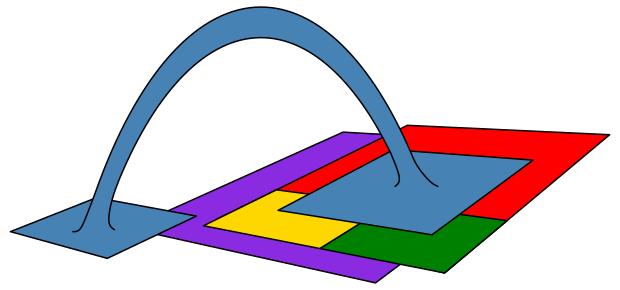
\includegraphics{bridge.png}
  \caption{A depiction of Peirce's Bridge for lines of identity}
  \footnotesize Source:\hspace{3pt}\url{https://commons.wikimedia.org/wiki/File:4CT_Inadequacy_Explanation.svg}
  \labfig{eg-bridge}
\end{marginfigure}

Thus he already identified the problem of readability stemming from having too
many lines or ``cables'' crossing eachother, a well-known concern in the design
of graphical programming languages\todo{Find reference}. This is to be opposed
to critics of the syntax of EG such as Quine, who invented a notation similar to
the lines of identity, and deemed it ``too cumbersome for practical
use''\todo{Find reference}. Also, the other proposed solution of having
so-called \emph{Bridges} is quite interesting, in that it makes the syntax of EG
\emph{three-dimensional}, in order to preserve the continuity of lines. A nice
illustration of the bridge is given in \reffig{eg-bridge}\sidenote{We found this
picture in the Wikipedia article on the \emph{four color theorem}
\cite{noauthor_four_2023}, which is no coincidence: according to Burch
\cite{sep-peirce}, \textit{``Peirce began to research the four-color map
conjecture, to work on the graphical mathematics of de Morgan's associate A. B.
Kempe, and to develop extensive connections between logic, algebra, and
topology, especially topological graph theory. Ultimately these researches bore
fruit in his existential graphs [...]''}. The Wikipedia article on Alfred Kempe
also mentions the following, to be connected with our multiset formalization of
EG \cite{noauthor_alfred_2023}: \textit{``Kempe (1886) revealed a rather marked
philosophical bent, and much influenced Charles Sanders Peirce. Kempe also
discovered what are now called multisets, although this fact was not noted until
long after his death.''}}.

\todo{ Use the following citation to explain how lines of identity are to be
  interpreted as quantifiers, where the term ``endoporeutic'', etymologically
  meaning ``from the outside to the inside'', refers to the relevance of the
  \emph{order} among quantifiers as to their meaning. }
  (\cite{peirce_prolegomena_1906}, p. 531):

\begin{quote}
  In the interpretation of Selectives it is often necessary to observe the rule
which holds throughout the System, that the Interpretation of Existential Graphs
must be \emph{endoporeutic}, that is, the application of a Graph on the Area of
a Cut will depend on the predetermination of the application of that which is on
the Place of the Cut.
\end{quote}
\newcommand{\tikzscale}[3]{
  \scalebox{#1}{
    \begingroup
      \tikzset{every picture/.style={scale=#2,baseline=(current bounding box.center)}}
      #3
    \endgroup}}
\renewcommand{\tikzfig}[3]{
  \tikzscale{#1}{#2}{\InputIfFileExists{./drawings/#3.tikz}{}{{\color{red}\colorbox{pink}{missingfile : #3}}}}}
\newcommand{\stkfig}[2]{\tikzfig{#1}{0.5}{#2}}

\usepackage{minted}

\usepackage{fontspec}
\usepackage{unicode-math}
\setmathfont{Libertinus Math}
\setmathfont{latinmodern-math.otf}[range=\multimap]
\setmathfont{STIXTwoMath-Regular.otf}[range={\Coloneq,"29D0,"25CF,"2AD0}]
% \setmathfont{LibertinusMath-Regular.otf}[range=\vdash]
% \setmathfont{LibertinusMath-Regular.otf}[range=\nvdash]
% \setmathfont{LibertinusMath-Regular.otf}[range=\vDash]
% \setmathfont{LibertinusMath-Regular.otf}[range=\nvDash]
% \setmathfont{LibertinusMath-Regular.otf}[range=\Vdash]
% \setmathfont{LibertinusMath-Regular.otf}[range=\nVdash]

\DeclareMathAlphabet{\mathcall}{OMS}{cmsy}{m}{n}

\newfontfamily{\subseteqfont}{LibertinusMath-Regular.otf}

\newcommand{\csup}{\symbol{"2AD0}}
\newcommand{\trhd}{\symbol{"29D0}}
\newcommand{\blackcirc}{\symbol{"25CF}}

\usepackage{newunicodechar}
\newunicodechar{⊆}{{\subseteqfont\subseteq}}
\newunicodechar{⧐}{\trhd}
\newunicodechar{●}{\blackcirc}
\newunicodechar{⫐}{\csup}

% Calligraphic font with \mathcb
% \DeclareFontFamily{U}{BOONDOX-calo}{\skewchar\font=45 }
% \DeclareFontShape{U}{BOONDOX-calo}{m}{n}{
%   <-> s*[1.05] BOONDOX-r-calo}{}
% \DeclareFontShape{U}{BOONDOX-calo}{b}{n}{
%   <-> s*[1.05] BOONDOX-b-calo}{}
% \DeclareMathAlphabet{\mathcb}{U}{BOONDOX-calo}{m}{n}
% \SetMathAlphabet{\mathcb}{bold}{U}{BOONDOX-calo}{b}{n}
% \DeclareMathAlphabet{\mathbcalboondox}{U}{BOONDOX-calo}{b}{n}

% Theorem environments

% \newtheorem{definition}{Definition}
% \newtheorem{theorem}{Theorem}
% \newtheorem{lemma}{Lemma}
% \newtheorem{corollary}{Corollary}
% \newtheorem{property}{Property}
% \newtheorem{proposition}{Proposition}
% \newtheorem{remark}{Remark}
% \newtheorem{notation}{Notation}
% \newtheorem{conjecture}{Conjecture}
% \newtheorem{condition}{Condition}

%%% Package config

% algorithm2e
\SetKw{Break}{break}
\SetKw{Continue}{continue}
\newcommand{\labproc}[1]{\label{proc:#1}}
\newcommand{\refproc}[1]{\texttt{\ref{proc:#1}}}

% enumitem
\setlist[description]{itemsep=0.5em}
\setlist[itemize]{align=left}

% tabularx
\newcolumntype{O}[1]{>{\setlength\hsize{#1\hsize}}c}
\newcolumntype{M}[1]{>{\small}m{#1\hsize}}
\newcolumntype{L}[1]{>{\raggedright\let\newline\\\arraybackslash\hspace{0pt}}m{#1}}
\newcolumntype{C}[1]{>{\centering\let\newline\\\arraybackslash\hspace{0pt}}m{#1}}
\newcolumntype{R}[1]{>{\raggedleft\let\newline\\\arraybackslash\hspace{0pt}}m{#1}}

% makecell
\renewcommand\theadfont{\bfseries\normalsize}

% xcolor
\usepackage{xcolor}
\definecolor{pos}{HTML}{C80000}
\definecolor{neg}{HTML}{0000C8}
\definecolor{hypo}{HTML}{007BFF}
\definecolor{conc}{HTML}{DC3545}
\definecolor{dvar}{HTML}{45A15A}
\definecolor{bubble}{HTML}{A0A0A0}
\definecolor{solved}{HTML}{DEFFCF}
\definecolor{genA}{HTML}{FFF8DD}
\definecolor{genB}{HTML}{FFEBFF}
\definecolor{hyp}{HTML}{FFEBFF}
\definecolor{hypnum}{HTML}{980098}
\definecolor{itsrc}{HTML}{0099ff}
\definecolor{itdst}{HTML}{b3e0ff}
\definecolor{ins}{HTML}{FFCCCC}
\definecolor{dcut}{HTML}{DADAD7}
\definecolor{dorange}{HTML}{FF6F00}
\definecolor{npcut}{HTML}{DFDFDE}
\definecolor{pbg}{HTML}{FFFFFF}
\definecolor{nbg}{HTML}{DFDFDE}
\definecolor{pfg}{HTML}{000000}
\definecolor{nfg}{HTML}{000000}
\definecolor{pistil}{HTML}{FFF344}

% prftree
\prflineextra=0em
\prflinepadbefore=0.5ex
\prflinepadafter=0.5ex
\prfrulenameskip=0.15em
\prflabelskip=0.35em
\prfdoublelineinterspace=0.001ex

\allowdisplaybreaks

% Custom LaTeX preamble for alectryon
% \usepackage{cmap} % fix search and cut-and-paste in Acrobat
% \usepackage{ifthen}
% \usepackage{alectryon}
% \usepackage{pygments}

%%% Notations

% Proof trees macros

\NewDocumentCommand{\rnm}{mO{}tr}
  {{\small$
    \IfBooleanT{#3}{\overline}{
      #1
    }^{#2}$}}

\NewDocumentCommand{\R}{oO{}trtd}{
  \expandafter\prftree\expanded{
    \IfBooleanT{#4}{[d]}
    \IfValueT{#1}{[r]{
      \unexpanded{\rnm{#1}}
      [#2]
      \IfBooleanT{#3}{r}
    }}
  }
}

\newcommand{\rsf}[1]{\text{\small$\mathsf{#1}$}}

\newcommand{\assum}{\prfassumption}
\newcommand{\summ}{\prfsummary}

% -------------------------------
% ---------- Notations ----------
% -------------------------------

% Long digression in the margin
\NewEnviron{digression}{
  \marginnote{
    \begin{kaodigression}
      \BODY
    \end{kaodigression}
  }
}

% Thick table lines
\makeatletter
\newcommand{\thickhline}{%
    \noalign {\ifnum 0=`}\fi \hrule height 1pt
    \futurelet \reserved@a \@xhline
}
\newcolumntype{"}{@{\hskip\tabcolsep\vrule width 1pt\hskip\tabcolsep}}
\makeatother

% \xleftrightarrow without mathtools
\makeatletter
\newcommand\xleftrightarrow[2][]{%
  \ext@arrow 9999{\longleftrightarrowfill@}{#1}{#2}}
\newcommand\longleftrightarrowfill@{%
  \arrowfill@\leftarrow\relbar\rightarrow}
\makeatother

% Small line break
\newcommand{\sbr}{~\\\vspace{-1em}}

\DeclareMathOperator*{\argmax}{arg\,max}
\DeclareMathOperator*{\argmin}{arg\,min}

\newcommand{\mt}{\qquad\mapsto\qquad}

\newcommand{\HOne}{\color{hypnum}\ding{172}}
\newcommand{\HTwo}{\color{hypnum}\ding{173}}
\newcommand{\HThree}{\color{hypnum}\ding{174}}
\newcommand{\HFour}{\color{hypnum}\ding{175}}
\newcommand{\HFive}{\color{hypnum}\ding{176}}

\newcommand{\Hyp}[1]{\colorbox{hyp}{#1}}

\newcommand{\bcase}{\textbf{Base case}}
\newcommand{\rcase}{\textbf{Recursive case}}

\newcommand{\Ceq}{\mathrel{\vcenter{\hbox{::}}{=}}}

\newrobustcmd\syneq{
  \mathrel{%
    \withkl{\kl[\syneq]}{%
      \cmdkl{\equiv}
    }%
  }%
}
\knowledge{\syneq}{notion}
\newrobustcmd\notsyneq{
  \mathrel{%
    \withkl{\kl[\syneq]}{%
      \cmdkl{\not\equiv}
    }%
  }%
}

\newcommand{\nats}{\mathbb{N}}

% Vertical and horizontal reflection in math mode
\newcommand{\hrefl}[1]{\text{\raisebox{\depth}{\scalebox{-1}[1]{$#1$}}}}
\newcommand{\vrefl}[1]{\text{\raisebox{\depth}{\scalebox{-1}[-1]{$#1$}}}}
\newcommand{\hvrefl}[1]{\text{\raisebox{\depth}{\scalebox{1}[-1]{$#1$}}}}

\newcommand{\sep}{\;\!;\!\;}

\newcommand{\defeq}{\triangleq}

\newcommand{\da}{\downarrow}
\newcommand{\ua}{\uparrow}

\knowledgenewrobustcmd\seq{\mathrel{\cmdkl{\Rightarrow}}}
\newcommand{\limp}{\supset}
\newcommand{\lsub}{\subset}
\newcommand{\lequiv}{\Leftrightarrow}

\newcommand{\mcirc}{\mathbin{⚬}}
\newcommand{\mdiam}{◇}

\knowledgenewrobustcmd\step[1]{\mathrel{\cmdkl{\rightarrow_{#1}}}}
\knowledgenewrobustcmd\steps[1]{\mathrel{\cmdkl{\rightarrow^{\ast}_{#1}}}}
\newrobustcmd\notstep[1]{\withkl{\kl[\step]}{\mathrel{\cmdkl{\nrightarrow_{#1}}}}}
\newrobustcmd\notsteps[1]{\withkl{\kl[\steps]}{\mathrel{\cmdkl{\nrightarrow^{\ast}_{#1}}}}}
\knowledgenewrobustcmd\nsteps[2]{\mathrel{\cmdkl{\rightarrow^{#1}_{#2}}}}
\knowledgenewrobustcmd\lstep[1]{\mathrel{\cmdkl{\rightharpoonup_{#1}}}}

\begin{scope}\knowledgeimport{sfl}
\knowledge{notion}
 | \step
 | \steps
 | \notstep
 | \notsteps
 | \nsteps
\end{scope}

\newrobustcmd\xlstep[1]{\withkl{\kl[\lstep]}{\mathrel{\cmdkl{\xrightharpoonup{#1}}}}}
\newrobustcmd\xstep[1]{\withkl{\kl[\step]}{\mathrel{\cmdkl{\xrightarrow{#1}}}}}
\newrobustcmd\xsteps[1]{\withkl{\kl[\step]}{\mathrel{\cmdkl{\xrightarrow{#1}\!\!\raisebox{3pt}[3pt]{\small$\ast$}~}}}}
\newrobustcmd\xinvstep[1]{\xleftrightarrow{#1}}

\newcommand{\deriv}[3]{#1 : #2 \steps{} #3}
\newcommand{\irule}[3]{#1 : #2 \step{} #3}
\newcommand{\rrule}[3]{#2 \step{#1} #3}

\newcommand{\sement}{\leq}
\newcommand{\semequiv}{\simeq}

\knowledgenewrobustcmd\bv{\cmdkl{\mathsf{bv}}}
\knowledgenewrobustcmd\fv{\cmdkl{\mathsf{fv}}}
\renewcommand{\emptyset}{⌀}
\newcommand{\subst}[3]{#1 \{ #2 / #3 \}}
\newcommand{\compr}[2]{\left\{#1 ~\middle|~ #2\right\}}
\newcommand{\compl}[1]{\overline{#1}}
\knowledgenewrobustcmd\fset[3]{\cmdkl{\{}#3\cmdkl{\}_{#1}^{#2}}}

\newcommand{\hypo}[1]{{\color{hypo} #1}}
\newcommand{\conc}[1]{{\color{conc} #1}}
\newcommand{\dvar}[1]{{\color{dvar} #1}}

\newcommand{\prov}[1]{\sststile{#1}{}}

\newcommand{\dmdual}[1]{\overline{#1}}

\newrobustcmd\hole{\square}
\newrobustcmd\cfill[2]{#1\select{#2}}

% Bubbles

\newcommand{\cham}{\textsc{Cham}}

\newcommand{\bubbleT}[1]{\llparenthesis~#1~\rrparenthesis}
\newcommand{\piq}[1]{\mathbin{\langle #1 \rangle}}

\newcommand*\circled[1]{\tikz[baseline=(char.base)]{
            \node[shape=circle,draw,fill=white,inner sep=2pt] (char) {#1};}}
\newcommand*\bcircled[1]{\tikz[baseline=(char.base)]{
            \node[shape=circle,draw,fill=solved,inner sep=2pt] (char) {#1};}}
\newcommand*\gAcircled[1]{\tikz[baseline=(char.base)]{
            \node[shape=circle,draw,fill=genA,inner sep=2pt] (char) {#1};}}
\newcommand*\gBcircled[1]{\tikz[baseline=(char.base)]{
            \node[shape=circle,draw,fill=genB,inner sep=2pt] (char) {#1};}}

\newcommand*\fillcircled[2]{\tikz[baseline=(char.base)]{
            \node[shape=circle,draw,fill=#1,inner sep=2pt] (char) {#2};}}


\newcommand{\bubble}[1]{\color{bubble}\circled{$#1$}}
\newcommand{\cbubble}[1]{\color{conc}\circled{$#1$}}
\newcommand{\hbubble}[1]{\color{hypo}\circled{$#1$}}

\newcommand{\bbubble}[1]{\color{bubble}\bcircled{$#1$}}
\newcommand{\hbbubble}[1]{\color{hypo}\bcircled{$#1$}}
\newcommand{\cbbubble}[1]{\color{conc}\bcircled{$#1$}}

\newcommand{\gAbubble}[1]{\color{bubble}\gAcircled{$#1$}}
\newcommand{\ggAbubble}[1]{\color{black}\gAcircled{$#1$}}
\newcommand{\hgAbubble}[1]{\color{hypo}\gAcircled{$#1$}}
\newcommand{\cgAbubble}[1]{\color{conc}\gAcircled{$#1$}}

\newcommand{\gBbubble}[1]{\color{bubble}\gBcircled{$#1$}}
\newcommand{\hgBbubble}[1]{\color{hypo}\gBcircled{$#1$}}
\newcommand{\cgBbubble}[1]{\color{conc}\gBcircled{$#1$}}

\newcommand{\bsheet}[1]{\colorbox{solved}{$#1$}}
\newcommand{\gAsheet}[1]{\colorbox{genA}{$#1$}}
\newcommand{\gBsheet}[1]{\colorbox{genB}{$#1$}}

\newcommand{\aint}[1]{\llfloor #1 \rrfloor}
\newcommand{\sint}[1]{\left\llbracket #1 \right\rrbracket}
\newcommand{\psint}[1]{\left\llbracket #1 \right\rrbracket^+}
\newcommand{\nsint}[1]{\left\llbracket #1 \right\rrbracket^-}

\newcommand{\identity}{\textsc{$\mathbb{I}$dentity}}
\newcommand{\flow}{\textsc{$\mathbb{F}$low}}
\newcommand{\resource}{\textsc{$\mathbb{R}$esource}}
\newcommand{\heating}{\textsc{$\mathbb{H}$eating}}
\newcommand{\membrane}{\textsc{$\mathbb{M}$embrane}}

\newcommand{\subsol}{\prec}

\newcommand{\deq}{\coloneq}
\newcommand{\ldef}[2]{#1 \deq #2}

\newcommand{\mix}{\,\mathbin{\cupdot}\,}
\newcommand{\J}{\mathbin{\rhd}}
\newcommand{\JB}{\mathbin{\RHD}}

\newcommand{\ltop}{\top}
\newcommand{\lbot}{\bot}
\newcommand{\lmeet}{\land}
\newcommand{\ljoin}{\lor}
\newcommand{\lexp}{\limp}
\newcommand{\lcoexp}{\lsub}

\newcommand{\soldepth}[1]{\left|#1\right|}
\newcommand{\bradepth}[1]{\left|#1\right|}
\newcommand{\soldual}[1]{\overline{#1}}

\newcommand{\Lattice}{\mathcall{L}}
\newcommand{\Heyting}{\mathcall{H}}
\newcommand{\Brouwer}{\mathcall{B}}
\newcommand{\HeytingBrouwer}{\mathcall{H\!B}}
\newcommand{\Boolean}{\mathcall{C}}
\newcommand{\ACVar}{\mathcall{X}}
\newcommand{\sementL}{\sement_{\Lattice}}
\newcommand{\sementH}{\sement_{\Heyting}}
\newcommand{\sementB}{\sement_{\Brouwer}}
\newcommand{\sementHB}{\sement_{\HeytingBrouwer}}
\newcommand{\sementC}{\sement_{\Boolean}}
\newcommand{\sementX}{\sement_{\ACVar}}

\newcommand{\sysB}{\kl[system B]{B}}
\newcommand{\sysBH}{B_{\!\Heyting}}
\newcommand{\sysBB}{B_{\!\Brouwer}}
\newcommand{\sysBHB}{B_{\!\HeytingBrouwer}}

\newcommand{\psintAnd}[3]{\bigwedge_{#1 \in #2}{\psint{#3}}}
\newcommand{\psintAndMix}[4]{\psintAnd{#1}{#2}{#1 \mix (#3 \seq #4)}}
\newcommand{\nsintOr}[3]{\bigvee_{#1 \in #2}{\psint{#3}}}
\newcommand{\nsintOrMix}[4]{\nsintOr{#1}{#2}{#1 \mix (#3 \seq #4)}}

\newcommand{\cS}{\mathcal{S}}

\newcommand{\dseq}{\mathbin{\trhd}}
\newcommand{\dtrans}[1]{\begingroup #1 \endgroup^{\scalebox{1.25}{$\bullet$}}}

\newcommand{\pol}[1]{\mathsf{pol}(#1)}

\newcommand{\imps}[1]{\mathrm{imp}(#1)}

% Existential Graphs

\knowledgenewrobustcmd\SA{\cmdkl{\textsc{\small SA}}}

\newcommand{\psheet}[1]{\color{pbg}{#1}}
\newcommand{\nsheet}[1]{\color{nfg}\colorbox{nbg}{$#1$}}
\newcommand{\pcut}[1]{\color{pfg}\fillcircled{pbg}{\color{pfg}$#1$}}
\newcommand{\ncut}[1]{\color{nfg}\fillcircled{nbg}{\color{nfg}$#1$}}

\newcommand{\opcut}[1]{\color{white}\fillcircled{white}{\color{black}$#1$}}
\newcommand{\oncut}[1]{\color{black}\fillcircled{black}{\color{white}$#1$}}

\knowledgenewrobustcmd\atoms{\cmdkl{\mathcal{A}}}

\knowledgenewrobustcmd\anodes{\cmdkl{\symbf{N_\alpha}}}
\knowledgenewrobustcmd\agraphs{\cmdkl{\symbf{G_\alpha}}}

\knowledgenewrobustcmd\bnodes{\cmdkl{\symbf{N_\beta}}}
\knowledgenewrobustcmd\bgardens{\cmdkl{\symbf{\Gamma_\beta}}}
\knowledgenewrobustcmd\bgraphs{\cmdkl{\symbf{G_\beta}}}

\knowledgenewrobustcmd\bcut[1]{\cmdkl{[}#1\cmdkl{]}}
\knowledgenewrobustcmd\bgarden[2]{#1 \mathbin{\cmdkl{\cdot}} #2}

\newcommand{\gdepth}[1]{\left|#1\right|}

\newcommand{\strans}[1]{\begingroup #1 \endgroup^{\scalebox{1.25}{$\bullet$}}}

\newcommand{\itsrc}[1]{\begingroup\setlength{\fboxrule}{0.8pt}\setlength{\fboxsep}{2pt}\color{itsrc}\fbox{\color{black}$#1$}\endgroup}
\newcommand{\itdst}[1]{\colorbox{itdst}{$#1$}}
\newcommand{\ins}[1]{\colorbox{ins}{$#1$}}
\newcommand{\dcut}[1]{\colorbox{dcut}{$#1$}}

\newcommand{\ljustif}{\mathbin{\succeq_0}}
\newcommand{\gjustif}{\mathbin{\succeq}}

\knowledgenewrobustcmd\subgraph{\mathrel{\cmdkl{\prec}}}

\newcommand{\westhook}[2]{
  \node[anchor=east,shape=diamond,draw,fill=white,inner sep=1pt] (#1) at (#2.west) {}
}
\newcommand{\easthook}[2]{
  \node[anchor=west,shape=diamond,draw,fill=white,inner sep=1pt] (#1) at (#2.east) {}
}
\newcommand{\northhook}[2]{
  \node[anchor=south,shape=diamond,draw,fill=white,inner sep=1pt] (#1) at (#2.north) {}
}
\newcommand{\southhook}[2]{
  \node[anchor=north,shape=diamond,draw,fill=white,inner sep=1pt] (#1) at (#2.south) {}
}
\newcommand{\northeasthook}[2]{
  \node[anchor=south west,shape=diamond,draw,fill=white,inner sep=1pt] (#1) at (#2.north east) {}
}
\newcommand{\northwesthook}[2]{
  \node[anchor=south east,shape=diamond,draw,fill=white,inner sep=1pt] (#1) at (#2.north west) {}
}
\newcommand{\southeasthook}[2]{
  \node[anchor=north west,shape=diamond,draw,fill=white,inner sep=1pt] (#1) at (#2.south east) {}
}
\newcommand{\southwesthook}[2]{
  \node[anchor=north east,shape=diamond,draw,fill=white,inner sep=1pt] (#1) at (#2.south west) {}
}

\newcommand{\ter}[2]{
\node[isosceles triangle,draw,minimum size=5pt,inner sep=0pt,fill=black] (#1) at (#2) {};
}
\newcommand{\coter}[2]{
\node[isosceles triangle,draw,minimum size=5pt,inner sep=0pt,fill=black,rotate=180] (#1) at (#2) {};
}
\newcommand{\terid}[2]{
\ter{#1}{#2}
\node[inner sep=0] (#1-in-top) at ($(#1.left corner) + (-1,+0.5)$) {};
\node[inner sep=0] (#1-in-bot) at ($(#1.right corner) + (-1,-0.5)$) {};
\node[inner sep=0] (#1-out) at ($(#1.apex) + (1,0)$) {};
\draw (#1.left corner) ..controls (#1.left corner) and ($(#1.left corner) + (0,0.55)$).. (#1-in-top);
\draw (#1.right corner) ..controls (#1.right corner) and ($(#1.right corner) - (0,0.55)$).. (#1-in-bot);
\draw ($(#1.apex) - (0.1,0)$) -- (#1-out);
}
\newcommand{\coterid}[2]{
\coter{#1}{#2}
\node[inner sep=0] (#1-out-top) at ($(#1.left corner) + (+1,-0.5)$) {};
\node[inner sep=0] (#1-out-bot) at ($(#1.right corner) + (+1,+0.5)$) {};
\node[inner sep=0] (#1-in) at ($(#1.apex) - (1,0)$) {};
\draw (#1.left corner) ..controls (#1.left corner) and ($(#1.left corner) - (0,0.55)$).. (#1-out-top);
\draw (#1.right corner) ..controls (#1.right corner) and ($(#1.right corner) + (0,0.55)$).. (#1-out-bot);
\draw ($(#1.apex) + (0.1,0)$) -- (#1-in);
}

\newcommand{\binder}[2]{
  \node[draw,circle,fill=black,inner sep=0,minimum size=3pt] (#1) at (#2) {};
}

% Flowers

\knowledgenewrobustcmd\entails[1]{\mathrel{\cmdkl{\vdash_{#1}}}}
\newrobustcmd\nentails[1]{\withkl{\kl[\entails]}{\mathrel{\cmdkl{\nvdash_{#1}}}}}

% \newcommand{\Nature}{\symbol{"2740}}
% \newcommand{\Culture}{\symbol{"273F}}
\knowledgenewrobustcmd\Nature{\cmdkl{\text{\ding{96}}}}
\knowledgenewrobustcmd\Culture{\cmdkl{\text{\ding{34}}}}

\knowledgenewrobustcmd\flower[2]{#1 \mathrel{\cmdkl{\csup}} #2}
\knowledgenewrobustcmd\garden[2]{#1 \mathbin{\cmdkl{\cdot}} #2}

\knowledgenewrobustcmd\flowers{\cmdkl{\mathbb{F}}}
\knowledgenewrobustcmd\gardens{\cmdkl{\mathbb{G}}}

\knowledgenewrobustcmd\interp[1]{\cmdkl{\lBrack}#1\cmdkl{\rBrack}}

\knowledgenewrobustcmd\chyp[2]{#1 \mathrel{\cmdkl{\succ}} #2}

\directlua{flower = require("flower")}
\newcommand{\DrawFlowers}[1]{\directlua{flower.many({#1})}}

\newcommand{\pissheet}[1]{\colorbox{pistil}{$#1$}}

\newcommand{\bx}{\mathbf{x}}
\newcommand{\by}{\mathbf{y}}
\newcommand{\bz}{\mathbf{z}}

\knowledgenewrobustcmd\fdepth[1]{\cmdkl{|}#1\cmdkl{|}}
\knowledgenewrobustcmd\cdepth[1]{\cmdkl{|}#1\cmdkl{|}}

\newcommand{\atomoccs}[1]{\mathcall{A}(#1)}
\newcommand{\vehicle}[1]{\mathcall{V}(#1)}
\newcommand{\anchor}[1]{\vrefl{\mathcall{V}}(#1)}
\newcommand{\lca}[2]{\mathsf{lca}(#1,#2)}

\newcommand{\cinter}{\mathbin{\bowtie}}
\newcommand{\cinterpos}{\mathbin{\stackon[1pt]{$\cinter$}{$\scriptstyle +$}}}
\newcommand{\cinterneg}{\mathbin{\stackon[1pt]{$\cinter$}{$\scriptstyle -$}}}
\newcommand{\sinter}{\mathbin{\hrefl{\propto}}}
\newcommand{\sinterpos}{\mathbin{\stackon[1pt]{$\sinter$}{$\scriptstyle +$}}}
\newcommand{\sinterneg}{\mathbin{\stackon[1pt]{$\sinter$}{$\scriptstyle -$}}}
\newcommand{\justi}{\mathbin{\hookrightarrow}}
\newcommand{\compat}{\mathbin{\da}}

\newcommand{\Action}[1]{\texttt{#1}}
\newcommand{\Proof}{\begingroup \textsc{Proof} \endgroup}
\newcommand{\Edit}{\begingroup \textsc{Edit} \endgroup}
\newcommand{\Navigation}{\begingroup \textsc{Navigation} \endgroup}

% First-order

\knowledgenewrobustcmd\vars{\cmdkl{\mathscr{V}}}
\knowledgenewrobustcmd\fsymbs{\cmdkl{\mathscr{F}}}
\knowledgenewrobustcmd\psymbs{\cmdkl{\mathscr{P}}}
\knowledgenewrobustcmd\arity{\cmdkl{\mathsf{ar}}}
\knowledgenewrobustcmd\dom{\cmdkl{\mathsf{supp}}}
\knowledgenewrobustcmd\terms{\cmdkl{\mathbb{T}}}
\knowledgenewrobustcmd\csts{\cmdkl{\mathbb{C}}}

\knowledgenewrobustcmd\upd[1]{\mathbin{\cmdkl{|_{#1}}}}
\newcommand{\update}[3]{#1 \upd{#2} #3}
\newcommand{\restr}[2]{#1\!\upd{#2}\!}
\newcommand{\idsubst}{\mathsf{1}}
\newcommand{\cstsubst}[1]{\overline{#1}}

\newcommand{\tvec}[1]{\vec{\mathbf{#1}}}

% Kripke

% \newcommand{\rewolF}[1]{\symbol{2702}(#1)}
\knowledgenewrobustcmd\rewolF[1]{\cmdkl{\text{\ding{95}}}(#1)}

\knowledgenewrobustcmd\kentails[1]{\mathrel{\cmdkl{\vDash_{#1}}}}
\newrobustcmd\notkentails[1]{\withkl{\kl[\kentails]}{\mathrel{\cmdkl{\nvDash_{#1}}}}}
\knowledgenewrobustcmd\kequiv[1]{\mathrel{\cmdkl{\vrefl{{\vDash}} {\vDash}_{#1}}}}

\knowledgenewrobustcmd\evaluation[1]{\cmdkl{$#1$-evaluation}}
\knowledgenewrobustcmd\consistent[1]{\cmdkl{$#1$-consistent}}
\knowledgenewrobustcmd\complete[1]{\cmdkl{$#1$-complete}}

\knowledgenewrobustcmd\eforces[3]{#1\mathrel{\cmdkl{\Vdash}}#2\,\cmdkl{[}#3\cmdkl{]}}
\newrobustcmd\neforces[3]{\withkl{\kl[\eforces]}{#1\mathrel{\cmdkl{\nVdash}}#2\,\cmdkl{[}#3\cmdkl{]}}}

\knowledgenewrobustcmd\access{\mathrel{\cmdkl{\leq}}}
\newrobustcmd\revaccess{\withkl{\kl[\access]}{\mathrel{\cmdkl{\geq}}}}

\knowledgenewrobustcmd\completion[1]{\cmdkl{\mathsf{Com}}(#1)}
\knowledgenewrobustcmd\ncompletion[2]{\cmdkl{\mathsf{Com}^{#2}}(#1)}

\newcommand{\tT}{\mathcall{T}}
\newcommand{\tU}{\mathcall{U}}

% Actema

\newrobustcmd\forw{
  \mathrel{%
    \withkl{\kl[\forw]}{%
      \cmdkl{\varoast}
    }%
  }%
}
\knowledge{\forw}{notion}

\newrobustcmd\back{
  \mathrel{%
    \withkl{\kl[\back]}{%
      \cmdkl{\varogreaterthan}
    }%
  }%
}
\knowledge{\back}{notion}

\newrobustcmd\para{
  \mathrel{%
    \withkl{\kl[\para]}{%
      \cmdkl{\varobar}
    }%
  }%
}
\knowledge{\para}{notion}

\DeclareMathOperator{\link}{\mathrel{@}}

\newcommand{\rever}{^*}
\newcommand{\phole}{\square}
\newcommand{\fhole}{\boxdot}
\newcommand{\ifill}[2]{#1\left\{#2\right\}}
\newcommand{\efill}[2]{#1\left[#2\right]}
\newcommand{\lint}[1]{\lfloor#1\rfloor}

\DeclareRobustCommand{\sys}[1]{\text{$\mathsf{#1}$}}
\newcommand{\pair}[2]{\left\langle #1, #2 \right\rangle}

\newcommand{\ra}{\rightarrow}
\newcommand{\FV}{\mbox{FV}}
\newcommand{\ocp}{\square_+}
\newcommand{\ocn}{\square_-}
\newcommand{\uA}{\select{A}}
\newcommand{\uB}{\select{B}}
\newcommand{\uC}{\select{C}}
\newcommand{\select}[1]{\fbox{$#1$}}
\newcommand{\stepto}{~~~~\mapsto~~~}
\knowledgenewrobustcmd{\inv}{\cmdkl{\mathsf{inv}}}
\newcommand{\uvars}{\mathsf{U}}
\newcommand{\lvar}{l}
\newcommand{\lvarp}{l^+}
\newcommand{\lvarn}{l^-}

\newcommand{\mother}{\mbox{\textsf{mother}}}
\newcommand{\rich}{\mbox{\textsf{Rich}}}
\newcommand{\human}{\mbox{\textsf{Human}}}
\newcommand{\mortal}{\mbox{\textsf{Mortal}}}
\newcommand{\socrates}{\mbox{\textsf{Socrates}}}

\newcommand{\injective}{\mbox{\textsf{injective}}}

\newcommand{\action}[1]{\textsf{#1}}
\newcommand{\process}[1]{\textsf{#1}}
\newcommand{\request}[1]{\texttt{#1}}
\newcommand{\trgoal}[1]{\llbracket #1 \rrbracket}
\newcommand{\traction}[1]{\llparenthesis #1 \rrparenthesis}
\newcommand{\subterms}[1]{\lfloor #1 \rfloor}

\newcommand{\ssreflect}{\textsc{SSReflect}}
\newcommand{\ltac}{$\mathcal{L}_{tac}$}

\knowledgenewrobustcmd\suc[1]{#1\cmdkl{\oplus}1}
% \newcommand{\suc}[1]{S(#1)}

% Type theory

\newcommand{\Prop}{\mathsf{Prop}}

\setmathfont{STIX2Math.otf}[range=\Coloneq]

\begin{document}


%----------------------------------------------------------------------------------------
%	BOOK INFORMATION
%----------------------------------------------------------------------------------------

\titlehead{}
\title{Deep Inference for Graphical Theorem Proving}
\author[PD]{Pablo Donato}
\date{January 22, 2024}
\publishers{}

%----------------------------------------------------------------------------------------

\frontmatter % Denotes the start of the pre-document content, uses roman numerals

%----------------------------------------------------------------------------------------
%	COPYRIGHT PAGE
%----------------------------------------------------------------------------------------

\makeatletter
\uppertitleback{\@titlehead} % Header

\lowertitleback{
	\textbf{Disclaimer} \\
	You can edit this page to suit your needs. For instance, here we have a no copyright statement, a colophon and some other information. This page is based on the corresponding page of Ken Arroyo Ohori's thesis, with minimal changes.
	
	\medskip
	
	\textbf{No copyright} \\
	\cczero\ This book is released into the public domain using the CC0 code. To the extent possible under law, I waive all copyright and related or neighbouring rights to this work.
	
	To view a copy of the CC0 code, visit: \\\url{http://creativecommons.org/publicdomain/zero/1.0/}
	
	\medskip
	
	\textbf{Colophon} \\
	This document was typeset with the help of \href{https://sourceforge.net/projects/koma-script/}{\KOMAScript} and \href{https://www.latex-project.org/}{\LaTeX} using the \href{https://github.com/fmarotta/kaobook/}{kaobook} class.
	
	\medskip
	
	\textbf{Publisher} \\
	First printed in May 2019 by \@publishers
}
\makeatother

%----------------------------------------------------------------------------------------
%	DEDICATION
%----------------------------------------------------------------------------------------

% \dedication{
% 	The ultimate meaning of logic is this ability to manipulate.
% 	\flushright -- Jean-Yves Girard.
% 	\small
% 	TODO: Move this as the epigraph of some chapter (either Introduction or
% 	Proof-by-Action)
% }


%----------------------------------------------------------------------------------------
%	OUTPUT TITLE PAGE AND PREVIOUS
%----------------------------------------------------------------------------------------

% Note that \maketitle outputs the pages before here
\maketitle

%----------------------------------------------------------------------------------------
%	ABSTRACT
%----------------------------------------------------------------------------------------

\chapter*{Abstract}

Proof assistants are software systems that allow for the precise checking of
mathematical reasoning. They can be general purpose (like Coq, Lean,
Isabelle...) or more specialized like EasyCrypt. They enable a level of accuracy
which certifies that no error can occur, but remain difficult to use.

We propose a new paradigm for constructing formal proofs through actions
performed in a graphical user interface (GUI), in order to enable a more
comfortable and intuitive use. Our paradigm builds upon direct manipulation
principles, combining both old (Proof-by-Pointing) and new (Proof-by-Linking)
interaction techniques that exploit recent advances in deep inference proof
theory. We implement the paradigm in a web-based GUI called Actema, which we
subsequently integrate into the Coq proof assistant by developing the coq-actema
plugin.

We then explore a series of deep inference proof systems that give more
structure to the notion of logical goal. These systems share the ability to
represent goals in two alternative ways: either textually through a standard
inductive syntax, or graphically using a metaphorical notation well-suited
to direct manipulation.

The first family of systems, called bubble calculi, is a topological
reformulation of the theory of nested sequents. It allows for efficient
sharing of hypotheses and conclusions among subgoals, facilitating the
factorization of both forward and backward proof steps. The second system,
called flower calculus, is an intuitionistic refinement of C. S. Peirce's
theory of existential graphs. Both types of systems are shown to be analytic
and fully invertible, making them amenable to proof automation techniques.

We finally go back to practical experimentation by designing and implementing
the Flower Prover, another web-based GUI for interactive proof building based on
the flower calculus. An innovative feature of the Flower Prover is that it works
well on modern mobile devices, thanks to its responsive layout and first-class
support for touch interactions.

% Proof assistants are software systems that allow for the precise checking of
% mathematical reasoning. They can be general purpose (like Coq, Lean,
% Isabelle...) or more specialized like EasyCrypt. They enable a level of accuracy
% which certifies that no error can occur, have given birth to a wide range of
% practical and theoretical works, and have been used in a wide range of
% applications. But they remain difficult to use.

% We propose a new paradigm of formal proof construction through actions performed
% in a graphical user interface, to enable a more comfortable and intuitive use.
% Our paradigm builds upon direct manipulation principles, combining both old
% (Proof-by-Pointing) and new (Proof-by-Linking) interaction techniques that
% exploit recent advances in deep inference proof theory. We implement this
% paradigm in a prototype of graphical user interface called Actema, using modern
% web-based technologies. We also design a generic protocol for plugging Actema on
% any proof system that supports first-order intuitionistic logic. This protocol
% is deployed inside the Coq proof assistant through the coq-actema plugin,
% offering users the ability to integrate graphical proofs into existing textual
% developments.

% % Then, driven by the will to integrate and improve the various interaction
% % techniques of Actema in a unified formalism, we explore a series of deep
% % inference proof calculi that give more structure to the notion of logical goal.
% % These calculi share the ability to be represented in two alternative ways:
% % either textually through a standard inductive syntax, or graphically through a
% % metaphorical notation well-suited to direct manipulation. In particular, we
% % propose to recast C.S. Peirce's theory of existential graphs as a system for
% % interactive, goal-oriented proof building. We support this claim with another
% % web-based prototype of graphical user interface, the Flower Prover, which has
% % the property of working well on touch-based devices of varying screen sizes.

% Then, driven by the will to improve the various interaction techniques of Actema
% in a unified formalism, we explore a series of deep inference proof systems that
% give more structure to the notion of logical goal. These systems share the
% ability to represent goals in two alternative ways: either textually through a
% standard inductive syntax, or graphically through a metaphorical notation
% well-suited to direct manipulation.

% The first family of systems, called bubble calculi, is an extension of the
% theory of nested sequents, that we reframe as local rewriting systems with a
% graphical and topological interpretation. Bubble calculi enable an efficient
% sharing of contexts between subgoals, making them well-suited to the
% factorization of both forward and backward reasoning steps in proofs. The second
% system, called flower calculus, is an intuitionistic refinement of C.S. Peirce's
% theory of existential graphs, understood as a system for interactive,
% goal-directed proof building. It provides more iconic and economical means of
% reasoning than bubble calculi, by exposing fewer inference rules that all work
% directly on the goals themselves, removing the need for logical connectives.
% % This should make the system easier to learn for users unfamiliar with symbolic
% % logic, by bridging the gap between statements and their proofs.
% Both types of systems are shown to be analytic and fully invertible, making them
% amenable to proof automation techniques.

% We finally go back to practical experimentation by designing and implementing
% the Flower Prover, another web-based prototype of GUI for interactive proof
% building based on the flower calculus. An innovative feature of the Flower
% Prover is that it works well on modern mobile devices, thanks to its responsive
% layout and first-class support for touch interactions.

% % The first family of systems, dubbed Bubble Calculi, is an extension of the
% % theory of nested sequents, that we reframe as local rewriting systems with a
% % graphical and topological interpretation. They enable a more efficient sharing
% % of contexts between subgoals, represented as so-called bubbles. Combined with
% % their perfect symmetry, this makes them well-suited to the factorization of both
% % forward and backward reasoning steps in proofs. We also show how they are able
% % to capture intuitionistic, dual-intuitionistic, bi-intuitionistic and classical
% % logic as fragments of a single calculus, that correspond to various physical
% % laws governing the porosity of bubbles.

% % The second system, dubbed Flower Calculus, is an intuitionistic refinement of
% % C.S. Peirce's theory of existential graphs, understood as a system for
% % interactive, goal-oriented proof building. It provides more iconic and
% % economical means of reasoning than Bubble Calculi, by requiring fewer inference
% % rules that all work directly on the goals themselves, removing the need for
% % logical connectives. To our knowledge, we provide the first proof of analyticity
% % of existential graphs in the literature, through a normalization-by-evaluation
% % argument with respect to Kripke models. Altogether, this should make the system
% % amenable both to new proof automation techniques, and interaction with users
% % unfamiliar with symbolic logic, bridging the gap between statements and their
% % proofs.

%----------------------------------------------------------------------------------------
%	TABLE OF CONTENTS & LIST OF FIGURES/TABLES
%----------------------------------------------------------------------------------------

\begingroup % Local scope for the following commands

% Define the style for the TOC, LOF, and LOT
%\setstretch{1} % Uncomment to modify line spacing in the ToC
%\hypersetup{linkcolor=blue} % Uncomment to set the colour of links in the ToC
\setlength{\textheight}{230\vscale} % Manually adjust the height of the ToC pages

% Turn on compatibility mode for the etoc package
\etocstandarddisplaystyle % "toc display" as if etoc was not loaded
\etocstandardlines % "toc lines as if etoc was not loaded

\setcounter{tocdepth}{1}
\tableofcontents % Output the table of contents

\listoffigures % Output the list of figures
\setcounter{tocdepth}{2}

% Comment both of the following lines to have the LOF and the LOT on different pages
\let\cleardoublepage\bigskip
\let\clearpage\bigskip

\listoftables % Output the list of tables

\endgroup

%----------------------------------------------------------------------------------------
%	MAIN BODY
%----------------------------------------------------------------------------------------

\mainmatter % Denotes the start of the main document content, resets page numbering and uses arabic numbers
\setchapterstyle{kao} % Choose the default chapter heading style

% \pagelayout{wide} % No margins
% \addpart{Preliminaries}
% \pagelayout{margin} % Restore margins

% \setchapterpreamble[u]{\margintoc}
\chapter{Introduction}
\labch{intro}

\epigraph{The ultimate meaning of logic is this ability to manipulate.}
{\textbf{Jean-Yves Girard}, \textit{The blind spot}, 2011}

% \paragraph{Formal manipulations}

\AP \intro{Proof assistants} (\reintro{PAs}) --- also called
\reintro{interactive theorem provers} (\intro{ITPs}) --- are software systems
that allow to both create and check the correctness of mathematical proofs. They
are based on the idea that mathematical knowledge can be represented
unambiguously inside \intro{proof formalisms} --- also called \reintro{proof
systems}, where the truth of a statement can be reduced to the mechanical
application of \kl{symbolic} manipulation rules. For instance, consider the
equation
$$4x + 6x = (12 - 2)x$$ 
While any mathematician would immediately recognize it as true, a middle school
student learning algebra would have to carry manually some computations to
convince herself (and her teacher) of its validity. A first step might consist
in applying the distributivity of multiplication over addition on the left-hand
side of the equation, yielding the new equation
$$(4 + 6)x = (12 - 2)x$$
Then, computing the sum on the left-hand side and the difference on the
right-hand side gives the final equation
$$10x = 10x$$
\AP which is trivially true. This is a very simple example, but it already shows
the two main aspects of \kl{proof formalisms}: on the one hand, they allow to
\emph{represent} mathematical statements in a formal language, here that of
equations between linear univariate polynomials; on the other hand, they allow
to \emph{manipulate} this representation in order to prove the statements, here
through \intro{rewriting rules} that transform a valid equation into another
valid equation.

Algebra lends itself particularly well to formalization, as it is arguably the
very study of the rules governing \kl{symbolic} manipulations in mathematics. It also
heavily relies on computations, which explains why it was the target of the
first, and to this day most popular application of computers to mathematics:
computer algebra systems.

However in this thesis, we are interested in improving the usability of
\kl{proof assistants}, which have a much broader scope than computer algebra
systems: their ambition is to enable the formalization on computers of virtually
\emph{any} kind of mathematics. Ultimately, the dream is to provide a platform
that helps humans in creating \emph{new} mathematics: both novel solutions and
proofs to existing problems, and brand new theories involving new types of
mathematical objects. This seemingly disproportionate ambition is not entirely
utopic: \AP it is based on the great discoveries of 19\textsuperscript{th} and
20\textsuperscript{th} century mathematicians and logicians, in the broad
research area now known as \intro{mathematical logic}.

\section{Proof theory}

\subsection{Mathematical logic}

\paragraph{Universal language}

\AP
At the dawn of the 20\textsuperscript{th} century, some mathematicians started
to realize that it may be possible to formalize not only specific branches of
mathematics like algebra with their own language, but the \emph{whole} of
mathematics in a single, universal language. This idea was first intuited in the
17\textsuperscript{th} century by Leibniz with his dream of a
\intro{characteristica universalis}, an ideal language in which all propositions
--- mathematical propositions, but also scientific propositions about the real
world, and even metaphysical propositions --- could be expressed and understood
unambiguously by every human. Also, Leibniz introduced the concept of a
\intro{calculus ratiocinator}, a systematic method for determining the truth of
any proposition expressed in the \kl{characteristica universalis}, providing a
definitive and objective way to settle any argument through simple
calculations\sidenote{Leibniz himself might have been inspired by his
predecessor Galileo, who famously declared that ``the universe [...] is written
in the language of mathematics'' \cite{assayer}.}.

\paragraph{Predicate logic and set theory}

\AP
The possibility of a universal language for mathematics became credible at the
dusk of the 19\textsuperscript{th} century, thanks to the works of logicians
like Boole, Frege and Peirce on one hand
\sidecite{Boole1854-BOOTLO-4,frege79,peirce_algebra_1885}, and mathematicians
like Cantor and Dedekind on the other hand
\sidecite{07557982-f50c-352d-bd73-3e2bc6403d4f}. The former laid the groundwork
for a formal account of deduction that greatly improved on Aristotle's
syllogistic, by inventing notations and rules that can express reasoning about
not only \emph{properties} of individuals, but also \emph{relations} between
them. The latter invented \intro{set theory}, which provided the first setting
where a general notion of \emph{function} or mapping could be rigorously
defined, a notion that became increasingly central in modern mathematics.

\paragraph{Foundations}

\AP
This formed the basis for a unification of many branches of mathematics on the
same \emph{foundation}: it was realized that with enough effort, every
mathematical structure could be encoded with the sets of Cantor, and all the
laws governing sets could be expressed with a finite number of \kl{axioms}
expressed in \intro{predicate logic}, i.e. the language and calculus of
relations devised by 19\textsuperscript{th} century logicians. This crystallized
into two famous axiomatic systems for \kl{set theory}: the \textit{Principia
Mathematica} of Russell and Whitehead \sidecite{russell25}; and Zermelo-Fraenkel
\kl{set theory} (\intro{ZF}, or \intro{ZFC} with the axiom of choice), which is
the most popular foundation nowadays because of its greater simplicity.

\paragraph{Truth and proofs}

\AP
An \intro{axiomatic system} specifies the formal language in which statements
about mathematical objects are expressed, as well as a collection of such
statements --- the \intro{axioms} --- that are taken to be true from the outset,
without further justification. One does not even need to speak about
\emph{truth} to define the system: although it can be a guiding intuition when
designing the system, the fact that \kl{axioms} denote true properties of
abstract objects in some ``mathematical universe'' is a particular philosophical
stance (platonism), which has nothing to do with concrete reasoning on the
formal representation.

\AP
Traditionally, the branch of \kl{mathematical logic} that tries to model the
``semantic'' content of \kl{axioms} through the notion of truth is called
\intro{model theory}. In this thesis, we are concerned with the construction of
formal proofs that derive the consequences of \kl{axioms} by pure ``syntactic''
manipulation, through the application of so-called \intro{inference rules}.
Accordingly, the branch of \kl{mathematical logic} studying this activity is
called \intro{proof theory}. We will still do a bit of \kl{model theory} in a few
places (\refsec{bubbles-soundness}, \refsec{Completeness}), but only as a means
to justify the properties of our syntax. Thus to avoid any unnecessary
philosophical commitment, we will only consider \kl{axioms} of a given system as
ordinary \emph{assumptions} that can be used in the course of reasoning, without
according any particular status to their truth. This is very much in line with
the \emph{formalist} school of thought in philosophy of mathematics, represented
by the great mathematician and main instigator of \kl{proof theory} David Hilbert.

\begin{emphpar}
\AP The real focus throughout this thesis is on the \emph{\kl{inference rules}}
used to build (correct) proofs from \kl{axioms}/assumptions. Those form the
theoretical basis for both the \emph{interactive creation}, and the
\emph{automatic checking} of formal proofs in \kl{proof assistants}. The branch
of \kl{proof theory} concerned with the study of \kl{inference rules} is called
\intro{structural proof theory}.
\end{emphpar}

\paragraph{Axiomatic systems} 

\AP
In the very beginnings of \kl{proof theory} in the 1920s, under the influence of
Hilbert, the axiomatic method was predominant, and thus \kl{proof systems} of
this era --- now called \reintro{Hilbert systems} --- featured very few
\kl{inference rules}. Almost all logical reasoning principles were encoded as
\emph{axiom schemas} involving generic \emph{propositional variables}. For
instance, the famous \intro{law of excluded middle} (\intro{LEM}), that states
that every proposition is either true or false, is expressed formally by the
schema
$$A \lor \neg A$$
Here, $\lor$ and $\neg$ are \kl{symbols} denoting the logical connectives of
\emph{disjunction} (``or'') and \emph{negation} (``not''), and $A$ is a
propositional variable that can be substituted with any concrete \emph{formula}
built from \emph{atomic propositions} and logical connectives. An atomic
proposition is typically a property of a mathematical object, that does not
involve any logical connective. An example of \emph{instance} of this schema
would be the proposition ``$n$ is prime or $n$ is not prime'' with $n$ some
natural number, which can be written formally as
$$\mathrm{prime}(n) \lor \neg\mathrm{prime}(n)$$
\AP Another related principle is the \intro{law of non-contradiction}, which states
that no proposition can be both true and false at the same time. It is expressed
by the schema
$$\neg (A \land \neg A)$$
where $\land$ is the \kl{symbol} denoting \emph{conjunction} (``and'').

\paragraph{Intuitionistic logic}

One motivating factor in the development of a new foundation for mathematics was
the discovery of strange theorems that defy intuition, like the existence of the
Weierstra{\ss} function which is continuous everywhere but differentiable
nowhere \sidecite{weirstrass_function}, or the Banach-Tarski paradox which
asserts that a ball can be decomposed and reassembled into two exact copies of
itself \sidecite{banach_sur_1924}. Some mathematicians like Brouwer and Weyl
rejected the truth of such theorems, on the basis that their proofs rely on
reasoning principles that are not \emph{constructive}\sidenote{This is true for
the Banach-Tarski paradox, which relies crucially on non-constructive
definitions of the concepts of partitions and equivalence classes \cite{175699}.
But for the Weierstra{\ss} function, it is possible to give it a constructive
definition with some efforts \cite{439047}.}. In particular, these principles
allow to prove the existence of objects satisfying certain properties without
ever providing a \emph{witness}, i.e. a concrete object that satisfies the
properties in question. This marked the birth of \emph{constructivism} in
philosophy of mathematics, whose most famous incarnation is Brouwer's
\emph{intuitionism}.

\AP
The original intuitionism of Brouwer was strongly opposed to any attempt at
formalizing mathematics, standing against both Frege and Russell's logicism that
saw mathematics as a mere branch of logic, and Hilbert's formalism that reduced
mathematics to a game of \kl{symbol} manipulation. However, this did not prevent
Heyting, one of Brouwer's students, from developing an axiomatic system in the
style of Hilbert and Frege, in an attempt to capture formally the objections of
Brouwer towards \intro{classical} logic --- i.e. the logic developed by
19\textsuperscript{th} century logicians that was at the heart of the new
\kl{set-theoretical} foundations. Heyting's system captures what is now called
\intro{intuitionistic} logic, which can be succinctly summarized as being
exactly \kl{classical} logic, but \emph{without} the \kl{law of excluded
middle}. Thus \kl{intuitionistic} logic is a generalization of \kl{classical}
logic, where propositions cannot be assigned a truth value \emph{a priori}: they
are only considered true if they can be proved with \emph{direct}, constructive
evidence.

To this day, there is no consensus among mathematicians as to which logic ---
\kl{intuitionistic} or \kl{classical} --- is the right one to found mathematics upon.
Since \kl{intuitionistic} logic is more restrictive than \kl{classical} logic, some
fundamental theorems of \kl{classical} mathematics do not hold anymore, requiring in
the worst cases to recreate entire branches of mathematics from scratch, like in
\emph{constructive analysis}. This explains why a large majority of
mathematicians still work in \kl{classical} logic, and are often even unaware of the
existence of constructive mathematics.

\begin{emphpar}
To account for this diversity, in this thesis we design \kl{proof systems} that
support \emph{both} \kl{classical} and \kl{intuitionistic} reasoning. Because every
theorem of \kl{intuitionistic} logic is also a theorem of \kl{classical} logic (but not
the converse), we will often focus first on the \kl{intuitionistic} ``kernel'' of our
systems, designing the \kl{classical} part as an extension of the former.
\end{emphpar}

\subsection{Structural proof theory}\labsubsec{structural-proof-theory}

\paragraph{Inference rules}

\AP
In \kl{Hilbert systems}, the only \kl{inference rule} is that of \intro{modus
ponens}, which is expressed formally with the following figure:
$$\R[\intro{mp}]{A}{A \limp B}{B}$$
Like \kl{axioms}, it is a \emph{schema} that involves generic propositional variables
$A$ and $B$, which may be \emph{instantiated} with arbitrary formulas. It can be
read from top to bottom as follows: for any propositions $A$ and $B$, if we have
a proof of $A$ and a proof of $A \limp B$, i.e. a proof that $A$ implies $B$,
then we can immediately derive a proof of $B$ by virtue of the rule, here
designated by the abbreviated name \kl{mp}. This reading of the rule
corresponds to a form of \intro{forward} reasoning: starting from the known
\emph{premises} that $A$ and $A \limp B$ are true, it \emph{necessarily} follows
that the \emph{conclusion} $B$ is true.

\AP
Conversely, one can also have a bottom-up reading of the rule: to build a proof
of any proposition $B$, one way to proceed is to come up with another
proposition $A$ such that both $A$ and $A \limp B$ are provable. This reading
corresponds to a form of \intro{backward} reasoning: we start from the conclusion
$B$ that we want to reach, also called the \intro{goal}, and try to find
\intro{subgoals} $A$ and $A \limp B$ that are provable, and hopefully simpler to
prove; then the rule guarantees that proving these \kl{subgoals} is \emph{sufficient}
to ensure the truth of the original \kl{goal}.

\kl{Forward} reasoning is typically how mathematicians write (informal) proofs on
paper, for the \emph{presentation} of their proofs to other mathematicians.
Indeed, it is more natural for humans to follow an argument by starting from its
premises, because the latter will always contain all the information required to
deduce the conclusion, the argument only serving as a means to explicate how
this information is combined. On the other hand, \kl{backward} reasoning is more
natural during the \emph{construction} phase of a proof, because the information
required to reach the conclusion (e.g. the proposition $A$ in the \kl{mp} rule)
is not yet known.

\paragraph{Natural deduction}

\AP
\kl{Axiomatic systems} can be relatively concise, in that many logics can be
expressed in them with a small number of \kl{axioms}. In return, they produce very
long and verbose formal proofs that are hard for humans to follow, and almost
impossible to come up with in most cases. In a series of seminars started in
1926, the Polish logician Łukasiewicz became one of the first to advocate for a
more \emph{natural} approach in \kl{proof theory}, that models more closely the way
mathematicians actually reason \sidecite{Jaskowski1934-JAKOTR-4}. A few years
later, in a dissertation delivered to the faculty of mathematical sciences of
the University of Göttingen \sidecite{gentzen_untersuchungen_1935}, the German
logician Gerhard Gentzen proposed independently his famous calculus of
\intro{natural deduction}.

\AP
This formalism follows the opposite approach to \kl{Hilbert systems}: it
features as few \kl{axioms} as possible, favoring the use of \emph{\kl{inference
rules}} to model the forms of reasoning found in mathematical practice. Those
are divided into two categories: \intro(natded){introduction rules}
\emph{define} the meaning of logical connectives, by prescribing how to prove
complex formulas from proofs of their components. Dually, \intro{elimination
rules} explain how to \emph{use} complex formulas, by giving a canonical way to
derive new conclusions from them. \reffig{calculi-NJ} shows the complete set of
\kl{natural deduction} rules for all connectives and quantifiers in
\kl{intuitionistic} logic, that was introduced by Gentzen under the name
\intro{NJ}\sidenote{Gentzen simultaneously introduced a \kl{natural deduction}
calculus named \intro{NK} for \kl{classical} logic, which is just \kl{NJ} with
an additional rule modelling the principle of \emph{indirect proof} --- i.e. the
possibility to prove any proposition $A$ by deriving a contradiction from its
negation $\neg A$ (\reffig{NK-ip}). Indeed, this principle can be expressed by
the formula $\neg\neg A \limp A$ which is strictly equivalent to the \kl{law of
excluded middle}, in the sense that $\neg\neg A \limp A$ is
(\kl{intuitionistically}) provable if and only if $A \lor \neg A$ is.}
\cite{gentzen_untersuchungen_1935}. The most simple example can be found in the
rules for the conjunction connective $\land$: the \kl(natded){introduction rule}
\kl{\land i} allows to build a proof of $A \land B$ by combining a proof of $A$
and a proof of $B$; while the \kl{elimination rules} \kl{\land e_1} and
\kl{\land e_2} allow to derive proofs of $A$ and $B$ from a proof of $A \land
B$.

\begin{figure*}
    \begin{framed}
  \begin{mathpar}
  \R[\rsf{\bot e}]
  {\bot}
  {A}
  \and
  \prftree[r][l]{\rsf{{\limp}i}}{\small[\prfref<HA>]}
  {\summ
    {\Gamma, \prfboundedassumption<HA>{A}}
    {B}}
  {A \limp B}    
  \and
  \R[\rsf{{\limp}e}]
  {A}
  {A \limp B}
  {B}
  \\
  \R[\rsf{\land i}]
  {A}{B}
  {A \land B}
  \and
  \R[\rsf{\land e_1}]
  {A \land B}
  {A}
  \and
  \R[\rsf{\land e_2}]
  {A \land B}
  {B}
  \\
  \R[\rsf{\lor i_1}]
  {A}
  {A \lor B}
  \and
  \R[\rsf{\lor i_2}]
  {B}
  {A \lor B}
  \and
  \prftree[r][l]{\rsf{\lor e}}{\small[\prfref<HA>,\prfref<HB>]}
  {A \lor B}
  {\summ
    {\Gamma, \prfboundedassumption<HA>{A}}
    {C}}
  {\summ
    {\Delta, \prfboundedassumption<HB>{B}}
    {C}}
  {C}
  \\
  \R[\rsf{\forall i}]
  {\summ{\Gamma}{A}}
  {\forall x. A}
  \and
  \R[\rsf{\forall e}]
  {\forall x. A}
  {\subst{A}{t}{x}}
  \and
  \R[\rsf{\exists i}]
  {\subst{A}{t}{x}}
  {\exists x. A}
  \and
  \R[\rsf{\exists e}]
  {\exists x. A}
  {\summ{\Gamma, A}{C}}
  {C}
  \vspace{1em}
  \end{mathpar}
  In the rules \rsf{\forall i} and \rsf{\exists e}, $x$ must not occur free in
  $\Gamma$ and $C$.
  \end{framed}

  \caption{\kl{Natural deduction} calculus \kl{NJ} for \kl{intuitionistic} logic}
  \labfig{calculi-NJ}
\end{figure*}

\begin{marginfigure}
  $$
  \prftree[r][l]{\intro{ip}}{\small[\prfref<H1>]}
  {\summ
    {\Gamma, \prfboundedassumption<H1>{\neg A}}
    {\bot}}
  {A}    
  $$
  \caption{Rule of indirect proof in \kl{natural deduction}}
  \labfig{NK-ip}
\end{marginfigure}

\begin{remark}
  Note that the rules for negation $\neg$ are not present in
  \reffig{calculi-NJ}: indeed, it is customary in \kl{intuitionistic} logic to define
  negation by $\neg A \defeq A \limp \bot$, identifying the negation of any
  proposition $A$ with its implying of a contradiction. Thus the rules for
  negation are subsumed by those for implication $\limp$ and absurdity $\bot$.
\end{remark}

\begin{marginfigure}
  $$
  \prftree[r][l]{\kl{{\limp}i}}{\small[\prfref<H1>]}
    {\R[\kl{{\limp}e}]
      {\R[\kl{\land e_1}]
        {\prfboundedassumption<H1>{A \land \neg A}}
        {A}}
      {\R[\kl{\land e_2}]
        {\prfboundedassumption<H1>{A \land \neg A}}
        {\neg A}}
      {\bot}}
    {\neg (A \land \neg A)}
  $$
  \caption{Proof of the \kl{law of non-contradiction} in \kl{natural deduction}}
  \labfig{PNC-NJ}
\end{marginfigure}

All logical reasoning principles that were \emph{axiomatized} in \kl{Hilbert
systems} can be \emph{derived} in \kl{natural deduction}. For example,
\reffig{PNC-NJ} shows a proof of the \kl{law of non-contradiction}, built
by \emph{composing} instances of rules from \reffig{calculi-NJ}. The composition
of a rule instance \rsf{r1} with another rule instance \rsf{r2} simply consists
in using the conclusion of \rsf{r1} as one of the premisses of \rsf{r2}.

\begin{figure*}
    \begin{framed}
  \textsc{Identity}
  \begin{mathpar}
  \R[\rsf{ax}]
  {A \seq A}
  \and
  \R[\rsf{cut}]
  {\Gamma \seq A}
  {\Delta, A \seq C}
  {\Gamma, \Delta \seq C}
  \vspace{1em}
  \end{mathpar}
  \textsc{Structural}
  \begin{mathpar}
  \R[\rsf{ex}]
  {\Gamma, A, B, \Delta \seq C}
  {\Gamma, B, A, \Delta \seq C}
  \and
  \R[\rsf{ctr}]
  {\Gamma, A, A \seq C}
  {\Gamma, A \seq C}
  \and
  \R[\rsf{wkn}]
  {\Gamma \seq C}
  {\Gamma, A \seq C}
  \vspace{1em}
  \end{mathpar}
  \textsc{Logical}
  \begin{mathpar}
  \R[\rsf{\bot L}]
  {\Gamma, \bot \seq C}
  \and
  \R[\rsf{{\limp}L}]
  {\Gamma \seq A}
  {\Delta, B \seq C}
  {\Gamma, \Delta, A \limp B \seq C}
  \and
  \R[\rsf{{\limp}R}]
  {\Gamma, A \seq B}
  {\Gamma \seq A \limp B}
  \\
  \R[\rsf{\land L_1}]
  {\Gamma, A \seq C}
  {\Gamma, A \land B \seq C}
  \and
  \R[\rsf{\land L_2}]
  {\Gamma, B \seq C}
  {\Gamma, A \land B \seq C}
  \and
  \R[\rsf{\land R}]
  {\Gamma \seq A}
  {\Delta \seq B}
  {\Gamma, \Delta \seq A \land B}
  \\
  \R[\rsf{\lor L}]
  {\Gamma, A \seq C}
  {\Delta, B \seq C}
  {\Gamma, \Delta, A \lor B \seq C}
  \and
  \R[\rsf{\lor R_1}]
  {\Gamma \seq A}
  {\Gamma \seq A \lor B}
  \and
  \R[\rsf{\lor R_2}]
  {\Gamma \seq B}
  {\Gamma \seq A \lor B}
  \\
  \R[\rsf{\forall L}]
  {\Gamma, \subst{A}{t}{x} \seq C}
  {\Gamma, \forall x. A \seq C}
  \and
  \R[\rsf{\forall R}]
  {\Gamma \seq A}
  {\Gamma \seq \forall x. A}
  \and
  \R[\rsf{\exists L}]
  {\Gamma, A \seq C}
  {\Gamma, \exists x. A \seq C}
  \and
  \R[\rsf{\exists R}]
  {\Gamma \seq \subst{A}{t}{x}}
  {\Gamma \seq \exists x. A}
  \vspace{1em}
  \end{mathpar}
  In the rules \rsf{\forall R} and \rsf{\exists L}, $x$ must not occur free in
  $\Gamma$ and $C$.
  \end{framed}

  \caption{\kl{Sequent calculus} \kl{LJ} for \kl{intuitionistic} logic}
  \labfig{calculi-LJ}
\end{figure*}

\paragraph{Sequent calculus}

\AP
In addition to the constructivists' objections, some doubts were raised by the
discovery of fatal flaws in early attempts at defining foundational
\kl{axiomatic systems}, the most famous one being the \emph{antinomy} of
Russell's paradox caused by the unrestricted axiom of comprehension in naive
\kl{set theory}. In order to restore absolute trust in the foundations of
(\kl{classical}) mathematics, Hilbert proposed in the early 1920s to prove
mathematically the \intro{consistency} of the \kl{axiomatic system} for arithmetic
introduced in 1889 by Peano\sidenote{A more involved \kl{axiomatic system} was
proposed one year earlier by Dedekind \cite{dedekind_nat}. Less known is that
Peirce had already published in 1881 an equivalent axiomatization of natural
numbers \cite{peirce_logic_1881}.}, i.e. that no contradiction can be derived
from Peano's axioms. Indeed, he believed that every mathematical truth could be
derived from the principles of arithmetic, thus reducing the problem of the
\kl{consistency} of mathematics to that of arithmetic. Moreover, Hilbert's program
was to be carried by \emph{finitist} means, without resorting to any reasoning
principle involving infinite collections --- which were at the heart of the
controversy started by constructivists. This was the initial impulse for
developing \kl{proof theory}, since it provided a mathematical definition of
``mathematical proofs'' as \emph{finite} sequences of \kl{symbols} satisfying
certain properties.

\AP
Gentzen's work on \kl{natural deduction} was an integral part of this program,
as an attempt to render the \emph{metamathematics} of \kl{proof theory} more
structured and elegant. However, he could not devise any argument for
\kl{consistency} in this framework. He thus set out to devise a new formalism
that would be a reformulation of \kl{natural deduction} with better mathematical
properties, such as \emph{symmetries}. This gave us \intro{sequent calculus},
which is widely regarded as the cornerstone for most developments in \kl{proof
theory} to this day. Gentzen introduced simultaneously \emph{two} \kl{sequent
calculi}: one for \kl{classical} logic called \intro{LK}, and one for
\kl{intuitionistic} logic called \intro{LJ}. Here we focus on the
\kl{intuitionistic} system \kl{LJ}, whose rules are shown in
\reffig{calculi-LJ}.

\AP
\kl{Sequent calculus} is based on the observation that some rules in \kl{natural
deduction} depend crucially on the use of \emph{hypotheses} that appear
``higher'' or earlier in the proof. The prototypical example is the
\kl(natded){introduction rule} \kl{{\limp}i} for implication: to prove $A \limp
B$, it suffices to prove $B$ under the assumption that $A$ is true. Then the
hypothesis $A$ is \emph{discharged} by the rule (bracket notation in
\reffig{calculi-NJ}), meaning that the conclusion $A \limp B$ holds
\emph{unconditionally}, without the assumption. In \kl{sequent calculus}, this
relation of provability of a conclusion $C$ under a
collection/\intro(sequent){context} of hypotheses $\Gamma$ is captured by the
expression $\Gamma \intro*\seq C$, called a \intro{sequent}. The
\kl(natded){introduction rule} \kl{{\limp}i} is then expressed by the so-called
\intro{right introduction rule} \kl{{\limp}R}, which keeps track of the full
\kl(sequent){context} of hypotheses by having \kl{sequents} as premiss and
conclusion, instead of just formulas. \kl{Right introduction rules} for other
connectives are also obtained straightforwardly from the corresponding
\kl(natded){introduction rules} in \kl{natural deduction}, by simply making the
\kl(sequent){contexts} $\Gamma$ and $\Delta$ always explicit.

\AP
Following the original presentation of Gentzen, \kl(sequent){contexts} are taken
to be \emph{lists} of formulas (``Sequenz'' in German), i.e. ordered collections
where repetitions are allowed. Still, we really want to see them as \emph{sets}
of formulas, since it is implicit in mathematical practice that:
\begin{enumerate}
\item the \emph{order} in which hypotheses are listed does not matter;
\item hypotheses may be used \emph{more than once} in a proof (as in
\reffig{PNC-NJ}).
\end{enumerate}
These two conventions are respectively captured by the \intro{structural rules}
\kl{xL} of \intro{exchange} and \kl{cL} of \intro{contraction} in
\reffig{calculi-LJ}. A third \kl{structural rule}, \kl{wL} for
\intro{weakening}, accounts for the presence of unused assumptions in some
proofs, by allowing the introduction of new hypotheses at will (with a top-down
reading of rules).

\begin{marginfigure}
  $$
  \R[\kl{{\limp}R}]
  {\R[\kl{cL}]
  {\R[\kl{\land L_1}]
  {\R[\kl{\land L_2}]
  {\R[\kl{{\limp}L}]
    {\R[\kl{ax}]
    {A \seq A}}
    {\R[\kl{ax}]
    {\bot \seq \bot}}
    {A, \neg A \seq \bot}}
  {A, A \land \neg A \seq \bot}}
  {A \land \neg A, A \land \neg A \seq \bot}}
  {A \land \neg A \seq \bot}}
  {\seq \neg (A \land \neg A)}
  $$
  \caption{Proof of the \kl{law of non-contradiction} in \kl{sequent calculus}}
  \labfig{PNC-LJ}
\end{marginfigure}

\AP The main difference between \kl{sequent calculus} and \kl{natural deduction}
lies in its splitting of \kl{elimination rules} into two parts: \intro{left
introduction rules}, and the \intro(rule){cut} rule \kl{cut}. As their name
indicates, \kl{left introduction rules} serve a purpose symmetric to \kl{right
introduction rules}: while the latter define how to introduce a connective in
the conclusion of a sequent, the former define how to introduce a connective in
one of its hypotheses. Then, the only way to \emph{use} such an hypothesis $A$
is through the \kl{cut} rule, which erases $A$ from the \kl{context} in the
conclusion of the rule, by justifying it with the proof of $A$ given as premiss.
The \kl{cut} rule can also be seen as a generalization of the \kl{modus ponens}
rule of \kl{Hilbert systems}, replacing the logical connective $\limp$ of
implication by the ``structural connective'' $\seq$ of sequents. The remaining
\intro(rule){axiom} rule \kl{ax} is in a sense dual to the \kl{cut} rule: while
the latter allows justifying a hypothesis by an identical conclusion, the
\kl{ax} rule allows justifying a conclusion by an identical
hypothesis\sidenote{It is not clear where the terminology ``axiom rule'' comes
from. It might be because hypotheses can be considered as \kl{axioms} in the
sense we introduced earlier, i.e. statements that we \emph{assume} to be true.
In any case, it would be a misattribution of category to consider the \kl{ax}
rule itself as an \kl{axiom}, and some authors like Girard call it the
\intro(sequent){identity rule} or \rsf{id} rule to avoid the confusion --- which
also coincides with the concept of \emph{identity morphism} in \kl{category
theory}.}. \reffig{PNC-LJ} shows a proof of the \kl{law of non-contradiction} in
\kl{LJ}.

% Both the \kl{cut} and \kl{ax} rules seem completely trivial. Yet surprisingly,
Gentzen managed to prove a powerful result called alternatively
\textit{Haupstatz}, \emph{fundamental theorem} (of \kl{proof theory}), or
\intro{cut-elimination}: every provable formula in \kl{sequent calculus} has a
\emph{cut-free} proof, i.e. a proof that does not make use of the \kl{cut} rule.
Intuitively, it can be understood as a formal justification for the possibility
to \emph{inline} proofs of lemmas, by seeing an instance of \kl{cut} on $A$ as a
way to invoke the lemma $A$ without duplicating its proof. Moreover, Gentzen's
proof of the Haupstatz is itself constructive: it describes an \emph{algorithm}
for transforming every \kl{sequent calculus} proof into a cut-free one. Thus the
\kl{cut} rule is said to be \intro{admissible}, in the sense that any provable
\kl{sequent} can be proved without it.

\AP An important consequence of \kl{cut-elimination}, which was the original
motivation of Gentzen, is the consistency of the logic (\kl{intuitionistic}
\kl{predicate logic} in the case of \kl{LJ}). This stems from the fact that all
rules apart from the \kl{cut} rule satisfy the \intro{subformula property}:
every formula $A$ appearing in the premisses is a \emph{subformula} of some
formula $B$ in the conclusion, i.e. $A$ already occurs inside $B$. Thus there
cannot exist a proof of the absurd \kl{sequent} $\seq \bot$, since the only formula
that is a subformula of $\bot$ is $\bot$ itself, and there is no rule instance
with $\seq \bot$ as conclusion that only contains $\bot$ in its premisses. The
\kl{subformula property} is the first occurrence of the concept of
\intro{analyticity} in \kl{proof theory}, and can be seen as a technical
realization of the philosophical notion of analyticity first applied to
propositions by Kant, and later to proofs in mathematics by Bolzano
\sidecite{bolzano}.

Unfortunately, the proof of \kl{cut-elimination} for the \kl{sequent calculus}
incorporating Peano's axioms, found by Gentzen a few years after proving
\kl{cut-elimination} for \kl{LJ} \sidecite{gentzen_widerspruchsfreiheit_1936}, is
not finitist: it makes use of a transfinite induction up to the ordinal
$\epsilon_0$. But the very ideas of \kl{cut-elimination} and \kl{analyticity} will have
far-reaching applications in \kl{proof theory} and beyond, including many of the
results presented in this thesis.

\paragraph{Deep inference}

\AP Many years after Gentzen's seminal work, at the advent of the
21\textsuperscript{th} century, Alessio Guglielmi introduced a new methodology
for designing \kl{proof formalisms} called \intro{deep inference}
\sidecite{Guglielmi1999ACO}. The idea was to overcome some limitations of
Gentzen formalisms while preserving their good properties, by allowing
\kl{inference rules} to be applied \emph{anywhere} inside formulas, instead of
only at the top-level of sequents\sidenote{In fact, Schütte had already proposed
a \kl{deep inference} system as early as 1977 \cite{schutte_proof_1977}, as did
Peirce one century before him with his \emph{\kl{entitative graphs}} (as we will
see in \refch{eg}). But the idea did not generate much interest at the times.}.
The first \kl{deep inference} system was the \intro{calculus of structures}
(\intro{CoS}), which can be succinctly described as a \intro{rewriting system}
on formulas. For instance, the following \intro{switch rule}, when read
bottom-up (i.e. in \kl{backward} mode), indicates that the formula $A \lor (B
\land C)$ may be rewritten into $(A \lor B) \land C$:
$$\R[\kl{s}]{S\select{(A \lor B) \land C}}{S\select{A \lor (B \land C)}}$$
\AP Importantly, the rule can be applied in any \emph{context} $S\hole$. A
\intro{context} $S\hole$ is simply a formula containing a single occurrence of a
special subformula $\hole$ called its \intro{hole}, which can be \emph{filled}
(i.e. substituted) with any formula $A$ to give a new formula $S\select{A}$.
This notion of \kl{context} serves two purposes:
\begin{itemize}
  \item it formalizes the ability of \kl{rewriting rules} to be applied at an
  arbitrary \emph{depth} inside expressions, while retaining all the information
  available in the surrounding \kl{context};
  \item it generalizes the \kl(sequent){contexts} $\Gamma, \Delta$ of
  \kl{sequent calculus}, by giving them the full structure of formulas instead
  of just flat lists of formulas. Indeed, a \kl{sequent} $\Gamma \seq C$ can be
  interpreted as the formula $\bigwedge \Gamma \limp C$, where $\bigwedge
  \Gamma$ denotes the conjunction of all the formulas in $\Gamma$.
\end{itemize}
Then, a proof of a formula $A$ in the \kl{calculus of structures} is not a
\emph{tree} of rule instances as in \kl{natural deduction} and \kl{sequent
calculus}, but a \emph{sequence} of rewritings $A \steps{} \top$ that reduces
$A$ to the trivially true \kl{goal} $\top$.

\AP
The \kl{calculus of structures}, as a \kl{rewriting system}, is closer to the
equational reasoning that mathematicians are accustomed to in algebra. The main
difference is that most rules (including the \kl{switch rule} \kl{s}) can only
be applied in a \emph{single} direction, because the premiss and conclusion are
not \emph{equivalent}\sidenote{In the standard system \kl{SKS} from where the
\kl{s} rule originates, every context is \emph{\kl(sfl){positive}}, in the sense that the
hole $\hole$ never occurs under a negation $\neg$ or left-hand side of an
implication $\limp$; otherwise the rule would need to be restricted to \kl{positive}
contexts to stay valid. See \refsec{eg-completeness} for more details on
\kl{SKS}.}. When the premiss and conclusion of a rule are equivalent, we say
that the rule is \intro{invertible}.

\begin{emphpar}
\emph{All} the \kl{proof formalisms} designed in this thesis are \kl{deep inference}
\kl{rewriting systems} in the style of the \kl{calculus of structures}.
\end{emphpar}

\section{Proof assistants}

\kl{Proof assistants} are a direct application of \kl{proof theory}, exploiting the
ability of programming languages to represent and manipulate arbitrary data
structures to give a concrete implementation of \kl{proof formalisms}. Crucially,
they open the possibility to \emph{automate} the construction and verification
of formal proofs, by acting on two fronts:
\begin{itemize}
  \item on the \textbf{human} side, the design of \emph{high-level interfaces}
  for representing and manipulating statements and proofs can bridge the gap
  between the low-level and very detailed proofs of formal logic, and the
  informal proofs of mathematicians;
  \item on the \textbf{machine} side, the design of \emph{algorithms} that both
  find proofs of given statements and ensure their correctness can --- to some
  extent\sidenote{For instance, it is well-known that the problem of provability
  in \kl{predicate logic} is \emph{undecidable}.} --- relieve mathematicians from the
  burdens of proof-writing and proof-checking.
\end{itemize}
Thus the advent of computers gave a new purpose to \kl{proof theory}, going beyond
its foundational role with the hope to support and change the everyday practice
of mathematicians.

\begin{emphpar}
In this thesis, we are concerned mostly with the \emph{human} side of the
equation: we aim to provide smoother means for the user to communicate her
intent to the \kl{proof assistant}, and conversely for the \kl{proof assistant}
to communicate its results and suggestions on how to solve problems.
\end{emphpar}

\subsection{Logical frameworks}

\paragraph{Type theory}

\AP
The ancestor of all \kl{proof assistants} was the \intro{Automath} project,
initiated by Nicolaas Govert de Bruijn as soon as 1967. Citing Geuvers
\sidecite{geuvers_proof_2009}:
\begin{quote}
[One] aim of the project was to develop a mathematical language in which all of
mathematics can be expressed accurately, in the sense that linguistic
correctness implies mathematical correctness. This language should be computer
checkable and it should be helpful in improving the reliability of mathematical
results.
\end{quote}
\AP
Thus the design of \kl{Automath} was focused on the automatic
\emph{verification} of proofs through \emph{linguistic} means. It introduced
many fundamental ideas that are still at work in many modern \kl{proof
assistants}, the most prominent being the use of a \intro{type theory} to encode
formal proofs.

\AP Contrary to \kl{predicate logic} in traditional \kl{proof theory}, \kl{type
theories} break the syntactic hierarchy imposed upon mathematical objects,
propositions and proofs, by giving them a uniform representation as so-called
\intro{terms} that can be assigned a \intro{type}. The assertion that a
\kl{term} $t$ has \kl{type} $T$ is usually written with the expression $t : T$,
which has come to be called a typing \intro{judgment} after Martin-Löf. For
instance, the \kl{judgment} $3 : \nats$ states that the \kl{term} $3$ has the
\kl{type} $\nats$ of natural numbers, and $1 + 1 = 2 : \Prop$ states that the
\kl{term} $1 + 1 = 2$ has the \kl{type} $\Prop$ of propositions.

\paragraph{First-order vs. higher-order}

\AP Almost all \kl{type theories} are \intro{higher-order}: they give a
first-class status to functions and predicates, by allowing them to take other
functions and predicates as arguments. This is because they are based on the
\intro{$\lambda$-calculus} of Alonzo Church
\sidecite{15897363-af72-3dac-82e6-fde144ad66c0}, an intensional theory of
\kl{higher-order} functions that is now considered to be the first functional
programming language in history. For instance in \emph{simply-typed}
\kl{$\lambda$-calculus} \sidecite{e4d9a073-5bba-3a5b-90d3-81832cd433e5}, one may
\kl{type} the \emph{sum operator} over sequences of natural numbers with the
\kl{judgment} $\lambda u. \lambda n. \sum_{i = 1}^{n}{u~i} : (\nats \to \nats) \to
\nats \to \nats$, where $\lambda u. \lambda n. \sum_{i = 1}^{n}{u~i}$ is a
\intro{$\lambda$-term} encoding the \kl{higher-order} function that takes a
sequence represented as a function $u : \nats \to \nats$ and a bound $n :
\nats$, and returns the sum of each of $u$'s values at index $1 \leq i \leq n$
encoded as the function application $u~i$.

\AP By contrast, the \kl{predicate logic} developed in the
19\textsuperscript{th} century and studied in traditional \kl{proof theory} is
\intro{first-order}: functions and predicates can only take so-called
\emph{first-order individuals} as arguments, which usually model
``non-functional'' mathematical objects like numbers and sets.

\begin{emphpar}
In this thesis, we exclusively study \kl{proof formalisms} for
\emph{\kl{first-order}} \kl{predicate logic} (``\intro{FOL}'' hereafter).
\end{emphpar}

We identified a few reasons for working in \kl{FOL}:
\begin{itemize}
  \item it is a standard and well-understood setting that has received a lot of
  attention, allowing us to exploit various existing works from the \kl{structural
  proof theory} literature, and even from some overlooked theories of
  19\textsuperscript{th} century logicians;
  \item by contrast, \kl{type theory} is a quite recent subject\sidenote{Almost 100
  years younger than \kl{FOL} if we ignore Russell's theory of types (1902), that was
  based on a \kl{set theory} encoded in \kl{FOL}.}, which explains why there is still a
  great diversity of \kl{type theories} that differ in subtle and often incompatible
  ways;
  \item \kl{FOL} is a common kernel of virtually every \kl{type theory}, making our work
  directly applicable to all present and future \kl{proof assistants};
  \item it is also a simpler setting, that is powerful enough to study the
  essential features of logical reasoning, without the idiosyncracies of \kl{type
  theories} aimed at capturing the full complexity of mathematics.
\end{itemize}

\paragraph{Curry-Howard correspondence}

\AP
De Bruijn came up with the revolutionary idea that propositions could themselves
be seen as \kl{types}, by having \kl{judgments} such as $~t : 1 + 1 = 2~$ where $t$
is a \intro{proof term} representing a proof of the proposition $1 + 1 = 2$.
This \intro{propositions-as-types} principle was rediscovered independently by
Howard in 1978 \sidecite{Howard1980-HOWTFN-2}, and developed further into a
\intro{proofs-as-programs} correspondence --- also called \reintro{Curry-Howard
correspondence} or \reintro{Curry-Howard isomorphism}\sidenote{In fact, Curry
had already noticed in 1958 a similar connection between the \kl{types} of
combinators in his \emph{combinatory logic}, and the \kl{axioms} of \kl{Hilbert
systems} for implication \cite{Curry1959-CURCLV} --- hence the mention of
Curry.} --- where \kl{$\lambda$-terms} in the simply-typed
\kl{$\lambda$-calculus} are put in one-to-one correspondence with proofs in the
implicational fragment of the \kl{natural deduction} system \kl{NJ} of Gentzen.

\AP Thus the core of \kl{type theory} is \emph{\kl{intuitionistic}} in nature,
and the \kl{Curry-Howard correspondence} has fostered many fruitful interactions
between computer science, logic and constructive mathematics, with \kl{proof
assistants} acting as a crucial tool and source of investigations. One
influential development in this direction has been the \intro{intuitionistic
type theory} of Martin-Löf (\intro{MLTT}), which formed the basis for the
implementation of many \kl{proof assistants} like \intro{NuPrl}, \intro{Alf},
and most recently \intro{Agda} \cite{geuvers_proof_2009}. A system closely
related to \kl{MLTT}, the \intro{calculus of inductive constructions}
(\intro{CoIC}), is also implemented in two leading \kl{proof assistants}:
\intro{Coq} \sidecite{the_coq_development_team_2022_7313584} and \intro{Lean}
\sidecite{10.1007/978-3-030-79876-5_37}. Following the \kl{proofs-as-programs}
correspondence, these systems support the creation of both proofs and programs
that manipulate and compute mathematical objects, by compiling everything down
to \kl{typed} \kl{terms}.

\subsection{Interfaces}

\paragraph{Elaboration}

\AP
\kl{Type theories} are the logical foundation for the \intro(PA){kernel} of
\kl{proof assistants}, i.e. the part of the system that is responsible for
checking formal proofs expressed in a \emph{terse}, \emph{machine-oriented}
format. But it quickly became clear that this was not enough to make \kl{proof
assistants} a viable alternative to paper proofs: de Bruijn estimates that it
takes a time factor of 20 to translate a paper proof into a formalized proof in
\kl{Automath} \sidecite{7a66996d195e4eba8c3fe5dc5bab8fc5}. This factor has been
estimated to be shrinkable to 4 in the \intro{Mizar} \kl{proof assistant}
\sidecite{debruijn_factor}, thanks to the design of high-level \emph{languages}
for representing mathematical statements and proofs, that sit on top of the core
logical theory\sidenote{In the case of \kl{Mizar}, a typed \kl{set theory} based
on \kl{FOL}.}. The process of compiling a high-level proof text into a low-level
\kl{proof term} is called \intro{elaboration}.

\paragraph{Statement languages}

Any \kl{proof assistant} must provide the two following features in its statement
language:

\begin{description}
  \item[Logical primitives] Naturally, one needs a way to write
  propositions formed with logical connectives and quantifiers. This is usually
  done in \kl{symbolic} form, either with a custom ASCII notation, or with
  Unicode characters corresponding to the standard \kl{symbols} in more modern
  \kl{proof assistants}. 
  \item[Mathematical notations] In addition to the logical primitives,
  one needs to be able to express mathematical objects and operations in the
  domain of interest, e.g. numbers and arithmetic operators. Contrary to the
  logical language that can be hardcoded once and for all in the \kl{proof
  assistant}, the mathematical language needs to be \emph{extensible} by the
  user, so that custom notations can be defined for new mathematical objects.
\end{description}

\begin{emphpar}
  In this thesis, we focus exclusively on the \emph{logical primitives}, because
  they are found universally in all types of mathematical reasoning. 
\end{emphpar}

\AP
We leave aside the question of providing domain-specific languages for
particular branches of mathematics, which is nonetheless as much important. It
has been tackled extensively in Ayers' thesis \sidecite{ayers_thesis}, and more
specifically in his framework \intro{ProofWidgets} for user-extensible,
interactive graphical notations in the \kl{Lean} \kl{proof
assistant}\sidenote{For a similar approach to \kl{ProofWidgets} in the context
of functional programming, see \cite{omar-filling-2021}.}
\sidecite{ayers_graphical_2021}. De Moura and Ullrich have also designed a
powerful macro system for \kl{Lean} 4, that supports the \kl{elaboration} of
abstract notations into \kl{terms} of the underlying \kl{type theory}
\sidecite{ullrich_beyond_2022}.

\paragraph{Proof languages}

Once one disposes of a convenient way to state mathematical propositions, comes
the question of how to efficiently write \emph{proofs} of these propositions.
There have been broadly two approaches in the design of high-level proof
languages:

\begin{description}[labelsep=0pt]
  \itemAP[\intro{Imperative}~]proof languages, like imperative programming languages,
  offer a set of \emph{commands} or instructions than can be given to the
  computer to modify some state stored in memory. The latter is called the
  \intro{proof state}, and corresponds to the \emph{partial} proof that is built
  by the system incrementally through the execution of commands. In the dominant
  paradigm, these commands are provided by the user in text form; since Robin
  Milner and the LCF theorem prover~\sidecite{doi:10.1098/rsta.1984.0067}, they
  are called \intro{tactics}. Proof files are literally \intro{proof scripts},
  that is the sequence of \kl{tactics} typed in by the user.
  
  \AP
  Contrary to imperative programming languages, the main execution paradigm for
  \kl{proof scripts} is \emph{interactive}: the user triggers commands one at a time,
  so that she can visualize the intermediate \kl{proof states} and determine the next
  steps to take. In most \kl{tactics}-based \kl{ITPs},
  % \sidenote{One notable exception is the \kl{Agda} proof assistant, where the proof
  % state is assimilated with the whole file being edited, which is itself a
  % partial \emph{program} in a dependently-typed programming language,
  % following the Curry-Howard correspondence.}
  only the \emph{statement} part of the \kl{proof state} is shown, in a so-called
  \intro{proof view} or \reintro{goal view}. This corresponds to the \kl{goals} that the
  user needs to prove, and each \kl{goal} is presented in the form of a \kl{sequent} $\Gamma \seq C$, where $C$ is the conclusion that must be reached under the
  assumptions in $\Gamma$. \kl{Tactics} generally apply to one \kl{goal} at a time, and
  the user can choose which \kl{goal} to \emph{focus} at any point during the
  interaction. When the set of \kl{goals} becomes empty, we say that the initial goal
  or conjecture has been \emph{solved}.

  \begin{remark}\labremark{tactics-rules}
    The transformations performed by \kl{tactics} can be more or less
  sophisticated. But, fundamentally, one finds elementary commands that
  correspond roughly to the \kl{inference rules}, generally of \kl{natural
  deduction} or \kl{sequent calculus}. For instance, a \kl{goal} $\Gamma\seq
  A\lor B$ (resp. $\Gamma\seq A\land B$) can be turned into either a \kl{goal}
  $\Gamma\seq A$ or a \kl{goal} $\Gamma\seq B$ (resp. into two \kl{goals}
  $\Gamma\seq A$ and $\Gamma\seq B$), corresponding to the rules \kl{\lor R_1}
  and \kl{\lor R_2} (resp. \kl{\land R}) of \kl{LJ} in their \kl{backward}
  reading (\reffig{calculi-LJ}).
  \end{remark}

  \kl{Coq} and \kl{Lean} are examples of state-of-the-art \kl{proof assistants} in the
  \kl{imperative} paradigm.
  
  \itemAP[\intro{Declarative}~]proof languages follow a different approach, by
  aiming to provide an \emph{explicit}, \emph{self-contained} description of the
  proof. Although a \kl{goal view} is still available to guide the user during the
  proof construction process, the finished proof must be readable
  \emph{statically} by a human, without relying on the \kl{ITP} to compute and
  display intermediate \kl{proof states}. Consequently, \kl{declarative} proofs are more
  verbose and take longer to type than their \kl{imperative} homologues. But since
  they contain more information, they have the advantage of being more
  \emph{robust} to slight changes to definitions or to the statement of the
  theorem being proved, and are generally easier to \emph{debug}. They can also
  be put in correspondence with some \kl{proof-theoretical} formalisms, usually
  Fitch-style \kl{natural deduction} \cite{geuvers_proof_2009}.
  
  \AP
  \kl{Agda}, \kl{Mizar} and \intro{Isabelle} (with its \intro{Isar} proof
  language \sidecite{isar}) are examples of state-of-the-art \kl{proof
  assistants} in the \kl{declarative} paradigm.
\end{description}

\begin{emphpar}
  In this thesis, we focus mostly on exploring new modalities of interaction in
  the \emph{\kl{imperative}} paradigm. Only in \refsubsec{flowers-unified} do we
  sketch a possible escape from the \kl{imperative}/\kl{declarative} dichotomy.
\end{emphpar}

\begin{remark}
In some rare cases, an additional \emph{natural language} layer is added on top
of the proof language, to be as close as possible to informal proofs. With the
recent development of large language models like GPT, such natural language
translations are becoming increasingly convincing (see e.g. Patrick Massot's
work in \kl{Lean} \cite{LeanIPAM}).
\end{remark}


\section{This thesis}

\subsection{Research goals}

% \paragraph{Interoperability}

% Existing \kl{proof assistants} can (almost) never \emph{interoperate}: a proof or
% theorem written in one system cannot be imported into a different system. This
% is unsatisfactory for many reasons, including fragmentation in the formal
% methods community, and duplication of effort instead of reuse. There have been
% many attempts in recent years to address this issue in the \emph{backend}:
% various pairs of systems are made to exchange formal results through
% translations between their input (high-level) and output (low-level) languages,
% or in some cases by translations to and from more universal languages (see e.g.
% \sidecite{proofcert,dedukti}).

\paragraph{Universal user interface}

% The interoperability problem can also potentially be approached from the
% \emph{front-end}.
Many kinds of logical manipulations such as discharging assumptions,
instantiating quantifiers, and composing lemmas, are conceptually universal;
yet, a user wishing to carry out such manipulations in a particular \kl{proof
assistant} must express the wish in terms of the specific proof language of the
system. A \emph{universal user interface} would instead allow performing such
manipulations directly on the \emph{\kl{goal}} itself, using physical,
reversible, and incremental \intro{actions} with immediate feedback. A sequence
of user \kl{actions} should then be representable in terms of any particular proof
language.

\paragraph{Direct manipulation}

\AP
This approach to user interfaces has been termed \intro{direct manipulation} by
Shneiderman in the 1980s \sidecite{shneiderman_direct_1983}. It is now at the
heart of virtually every modern user interface and is arguably the major factor
in the \emph{personal computing revolution}. Indeed, it has opened the use of
computing devices to a much wider audience, by allowing users to interact with
them in an intuitive way that resembles interactions with physical objects in
the real world. According to Shneiderman, this contrasts with the
\emph{command-line} paradigm, where users need to memorize a complex command
language that often varies from one software to another within the \emph{same}
domain. This induces an unnecessary cognitive burden for newcomers, especially
those unfamiliar with textual interfaces, which constitute the majority of users
of computing devices nowadays; to the point that the hurdle is too great to
overcome for most potential users.

Unfortunately, the user interfaces of state-of-the-art \kl{proof assistants} are
largely stuck in the pre-80s era of command-line interfaces, making them
reserved to an audience of highly motivated, computer-savvy individuals. One
could argue that like programming languages, this is due to their inherent
\emph{abstraction} capabilities, that can only be captured through the
\kl{symbolic} power of language; hence that this state of fact is unavoidable,
and can only be solved through the addition (or improvement) of computer science
curricula in primary and secondary education. We do not agree with this
conception: we believe that the current state of user interfaces in \kl{ITPs} is
one of the major obstacles to their wider adoption in the mathematical
community, both by professional researchers, teachers, and novice students
alike.

\begin{emphpar}
  Our first main working hypothesis is that the \kl{direct manipulation}
  paradigm is not only possible, but also \emph{crucial} for building formal
  proofs in \kl{ITPs}, if they are to become a viable alternative to paper
  proofs in mathematics.
\end{emphpar}

In fact, following the \kl{proofs-as-programs} correspondence, we also believe
that this applies (to some extent) to \emph{programming}, and that it is only a
matter of time before direct manipulation becomes viable for building
(general-purpose) programs, in the spirit of \emph{visual programming
languages}. We do not explore this direction in this thesis, but it is one of
our hopes that some of the techniques we develop will apply to programming as
well; and one of the reasons why we chose to focus so much on
\emph{intuitionistic} logic.

\paragraph{Graphical deep inference}

\AP
A first attempt to design \kl{direct manipulation} principles for interactive
proof building was made in the 90s by the team of Gilles Kahn at Inria, where
they coined the \intro{Proof-by-Pointing} (\intro{PbP}) paradigm
\sidecite{PbP}. The idea was to synthesize complex \kl{tactics} from the simple
act of \emph{pointing} at specific locations inside expressions occurring in the
\kl{goal}, typically with a mouse cursor. More recently
\sidecite{Chaudhuri2013}, Kaustuv Chaudhuri proposed a variation on this idea
called \intro{subformula linking} (\intro{SFL}) or \intro{Proof-by-Linking}
(\intro{PbL}), where instead of selecting expressions in isolation, one can
\emph{link} two of them together to make them interact.

In both cases, the expressions considered were logical formulas and the
associated actions chains of inferences in \kl{FOL}. Importantly, both paradigms rely
on the use of \emph{\kl{deep inference}}, since the user can point at subformulas
that occur at an arbitrary depth inside the \kl{goal}. This is in contrast with the
basic commands found in the proof languages of \kl{ITPs}, where the user can only
designate formulas appearing at the top-level of sequents\sidenote{A notable
exception is the \texttt{rewrite} \kl{tactic} of \kl{imperative} proof languages, where
the user can specify \emph{patterns} to designate particular occurrences of a
term $t$ that are to be rewritten into an equal term $u$, usually thanks to an
assumed equation $t = u$. But coming up with such patterns is a lot slower than
directly \emph{pointing} at the locations of interest onscreen.}. While the
semantics of \kl{PbP} \kl{actions} is still based on the \emph{shallow} \kl{inference rules} of
\kl{sequent calculus}, \kl{PbL} fully embraces the \kl{deep inference} paradigm by relying on
\kl{CoS}-style \kl{rewriting rules}.

\begin{emphpar}
  \AP All the works presented in this thesis can be seen as a direct
  continuation of the research programme initiated by \kl{PbP} and \kl{PbL}. The
  aim is to \emph{replace} textual proof languages with \emph{gestural
  \kl{actions}} performed directly upon \emph{\kl{goals}} in a \intro{graphical
  user interface} (\intro{GUI}). To be as general as possible, we call such a
  paradigm \intro{Proof-by-Action} (\intro{PbA}).
\end{emphpar}

\paragraph{Proof exploration}

Note that we believe such a replacement to be useful mostly during the
\emph{construction} or \emph{writing} phase of proofs. Quoting Shneiderman
\cite{shneiderman_direct_1983}:
\begin{quote}
  The pleasure in using these systems stems from the capacity to manipulate the
object of interest directly and to generate multiple alternatives rapidly.
\end{quote}
Thus in the context of \kl{ITPs}, the major advantage of a (well-designed) \kl{GUI} in the
\kl{PbA} paradigm would be to enable the \emph{rapid exploration} of multiple paths
towards the construction of a complete proof. But once a proof has been found,
the \emph{dynamic} sequence of \kl{actions} that led to it could be ``compiled'' into
a \emph{static}, textual representation of the proof in the favorite proof
language of the user, to facilitate the \emph{reading} phase.

As for the \emph{modification} phase of proofs, the \kl{PbA} paradigm requires a
way to navigate and edit directly a recorded sequence of \kl{actions}, and possibly a
mechanism for mapping parts of a static proof object to the \kl{actions} that
generated them.

\begin{emphpar}
  In this thesis, we leave the question of \kl{proof evolution} in \kl{PbA} ---
  i.e. the design of interfaces for the reading and modification phases, that
  support a smooth interaction with the writing phase --- for future work. A
  more detailed discussion can be found in \refsubsec{proof-evolution}.
\end{emphpar}

\paragraph{Iconicity}

% The dominant paradigm for proof formalisms is \emph{linguistic} in nature:
% mathematical objects and assertions about them are represented in a formal
% language of propositions, also called \emph{formulas}, understood as a (usually
% infinite) set of strings of symbols.

Contrary to a common misconception among logicians, Leibniz did not conceive of
his \kl{characteristica universalis} as a \kl{symbolic} language, but rather as an
\emph{\kl{iconic}} one \sidecite[][Chpt.~3]{logique_leibniz}:
\begin{quote}
    The true ``real characteristic'' [...] would express the composition of
    concepts by the combination of signs representing their simple elements,
    such that the correspondence between composite ideas and their symbols would
    be natural and no longer conventional. [...] This shows that the real
    characteristic was for him an ideography, that is, a system of signs that
    directly represent things (or, rather, ideas) and not words.
\end{quote}
This is to be compared to Frege's \textit{Begriffsschrift}, a graphical,
two dimensional language and calculus of ``pure thought'', whose name has
repeatedly been translated as \emph{ideography}
\sidecite{Frege1952-FRETFT,Frege1999-FRELUL}.

\AP
Following the seminal work of Charles Sanders Peirce in
\intro{semiotics}\sidenote{\kl{Semiotics} is the systematic study of sign
processes and the communication of meaning.}, we define an \intro{iconic}
language as one whose signs are mainly \reintro{icons}, i.e. signs that
\emph{resemble} or share qualities with the objects they denote. This is to be
contrasted with \intro{symbolic} languages where most signs are just
\reintro{symbols}, i.e. signs that \emph{conventionally} denote their objects.
In his systematic usage of \emph{triads} of concepts, Peirce identified a third
kind of sign, \emph{indexes} \sidecite{atkin_peirces_2023}:
\begin{quote}
  if the constraints of successful signification require that the sign reflect
  qualitative features of the object, then the sign is an icon. If the
  constraints of successful signification require that the sign utilize some
  existential or physical connection between it and its object, then the sign is
  an index. And finally, if successful signification of the object requires that
  the sign utilize some convention, habit, or social rule or law that connects
  it with its object, then the sign is a symbol.
\end{quote}
\AP He even went further by analyzing \kl{icons} into another
trichotomy\sidenote{Actually he only applied this trichotomy to pure \kl{icons}
devoid of any indexical elements, that he called \emph{hypo-icons}.}:
\emph{images} that depend on simple quality; \intro{diagrams}, who share
\emph{structural} relations among their constituents that are analogous to that
of their object; and \intro{metaphors}, that denote features of their object by
relating them to features of another object \sidecite{legg_problem_2008}.

Interestingly, Peirce held that mathematics relies mostly on
\emph{\kl{diagrammatic}} thinking --- observation of, and experimentation on,
\kl{diagrams} \sidecite[][Chpt.~6]{Hookway1985-HOOP-2}. This agrees with the
contemporary practice of mathematics: indeed, there is an increasing number of
areas in mathematics --- the most prominent one being \intro{category theory}
--- where the heart of a proof lies in the dynamical construction of a
\emph{\kl{diagram}} capturing the structure of interest in given mathematical
objects. The natural language proof text is often just a means to explicit the
meaning or intuition behind the \kl{diagrammatic} manipulations, or simply a
retranscription of the commentary that the mathematician would give when
unfolding the construction on a blackboard.

\AP
If one views logic as one particular type of mathematical reasoning --- albeit
one that is omnipresent in all branches of mathematics, then it is only natural
to expect that some \kl{diagrammatic} system should exist for it, that can
express in the most natural way most (if not all) logical arguments. This is the
\emph{\kl{iconicity}} thesis of Peirce, which motivated his inquiry into what is
arguably the first \kl{diagrammatic} \kl{proof system} in history: the
\intro{existential graphs} (\intro{EGs}). This will be the subject of
\refch{eg}, and the basis for the development of a \emph{\kl{metaphorical}}
\kl{proof system} in \refch{flowers}.

\begin{emphpar}
  Our second main working hypothesis exploited in the second part of this
  thesis, is that \kl{iconic} representations of logical \emph{statements}, and the
  proofs that result from their manipulation, can play a crucial role in the
  design of intuitive proof building interfaces.
\end{emphpar}

\subsection{Contributions}

This thesis proposes several contributions toward the research goals highlighted
above.

\paragraph{Symbolic manipulations}
  
In the first part of this thesis, we substantiate the \kl{PbA} paradigm in the
context of traditional representations of \kl{goals}, by presenting a number of
techniques based on the \kl{direct manipulation} of \emph{\kl{symbolic}} formulas in
sequents.

\AP We start in \refch{pba} with an introduction to \kl{PbP} and \kl{PbL}, by
describing how to reason with logical connectives, quantifiers and equality
through \emph{click} and \intro{drag-and-drop} (\intro{DnD}) \kl{actions} in a
prototype of \kl{GUI} called \intro{Actema}. In particular, \kl{DnD}
\kl{actions} can be seen as a generalization of both the \texttt{apply} and
\texttt{rewrite} \kl{tactics} of \kl{imperative} proof languages.

In \refch{sfl}, we ground the semantics of \kl{DnD} \kl{actions} in \kl{deep
inference} \kl{proof theory}, by designing an \kl{intuitionistic} variant of the
\kl{CoS} for \kl{subformula linking} introduced by Chaudhuri in \cite{Chaudhuri2013}.
Our approach differs from Chaudhuri's mainly through our notion of
\emph{\kl(sfl){valid} \kl{linkage}}, which filters out unproductive \kl{DnD}
\kl{actions} by restricting them to \emph{\kl{unifiable}} subformulas.

In \refch{advanced}, we present more advanced techniques in the \kl{PbA}
paradigm, that handle pervasive forms of reasoning in mathematical practice such
as the use of \emph{definitions}, reasoning by \emph{induction}, and the
\emph{simplification} of expressions through automatic computation. This is
illustrated through a few case studies of basic logical and mathematical
problems.

In \refch{sfl-classical}, we investigate an extension of \kl{PbA} to \kl{sequents}
with \emph{multiple} alternative conclusions, as opposed to the
\emph{single}-conclusion \kl{sequents} found in the interface of almost every
\kl{ITP}. We argue that the use of \kl{direct manipulation} greatly facilitates
the management of multiple conclusions, and introduce a so-called
\emph{\kl(dnd){parallel}} \kl{interaction operator} to model reasoning in \kl{classical}
logic that involves the interaction of two conclusions.

\AP
Lastly in \refch{plugin}, we present \intro{coq-actema}, a plugin that
integrates the \kl{Actema} web application as an interactive \kl{proof view} in
\kl{Coq}. We focus on the architecture and interaction protocols that connect
the different components of the system, and give an overview of the
\kl{elaboration}/compilation strategy that turns graphical \kl{actions} performed in
\kl{Actema} into \kl{Coq} \kl{proof terms}. We also discuss current shortcomings
of our approach and future directions for improvement, in particular concerning
the question of \kl{proof evolution}.

\paragraph{Iconic manipulations}
  
In the second part of this thesis, we explore a series of \kl{deep inference}
\kl{proof systems} that give more structure to the notion of logical
\emph{\kl{goal}}. These systems share the ability to represent \kl{goals} in two
alternative ways: either \emph{textually} through a standard inductive syntax,
or \emph{graphically} through a \kl{metaphorical} notation well-suited to
\kl{direct manipulation}. The first can be used as a machine representation in
the backend of an \kl{ITP}, and the latter as the substrate for \kl{GUIs} in the
frontend.

\begin{description}
  \itemAP[Bubble calculi] In the first two chapters, we introduce a family of
  systems called \intro{bubble calculi}. They are an extension of the theory of
  \intro{nested sequents} first introduced by Brünnler
  \sidecite{brunnler_deep_2009}, that we reframe as local \kl{rewriting systems}
  with a graphical and topological interpretation. \kl{Bubble calculi} enable an
  efficient sharing of contexts between \kl{subgoals}, making them well-suited
  to the factorization of both \kl{forward} and \kl{backward} reasoning steps in
  proofs.

  \AP \refch{bubbles} presents the \emph{asymmetric} \kl{bubble calculus}
  \kl{BJ} for \kl{intuitionistic} logic, modelled after the \emph{asymmetric}
  \kl{sequents} of the \kl{intuitionistic} \kl{sequent calculus} \kl{LJ} of
  Gentzen. It introduces the \kl{metaphor} of \intro{bubbles} as a way to
  \kl{iconically} represent the separation and sharing of contexts between
  different \kl{subgoals}.

  \AP \refch{bubbles-symm} refines \kl{BJ} into a more general and symmetric
  calculus for \kl{classical} logic called \intro{system~B}, where \kl{bubbles}
  can be \emph{\kl(bubble){polarized}} in addition to formulas.
  \kl{Intuitionistic}, \kl{dual-intuitionistic} and \kl{bi-intuitionistic} logic
  can be recovered as fragments of \kl{system~B}, by forbidding certain
  \kl{inference rules} that characterize the \emph{porosity} of bubbles. We also
  devise a fully \kl{invertible} variant of \kl{system~B}, that we conjecture to
  be complete.
  
  \item[Existential graphs] In the last two chapters, we study two systems based
  on the \kl{existential graphs} of Peirce, that allow us to achieve \emph{full
  \kl{iconicity}}: every logical construction has an associated \kl{icon}, and thus there
  is no use anymore for the connectives and quantifiers of \kl{symbolic} formulas.
  Hopefully, this shall remove a first barrier in the learning of formal logic,
  which lies in the \emph{arbitrary} correspondence between \kl{symbols} and their
  meaning.

  In \refch{eg}, we give a complete review of Peirce's original systems of
  \kl{EGs} for propositional and \kl{first-order} \kl{classical} logic, which
  have been consistently neglected in the \kl{proof theory}
  literature\sidenote{One reason might be that \kl{EGs} have been invented at
  the end of the 19\textsuperscript{th} century, \emph{before} the birth of
  \kl{proof theory} as a discipline in the 1920s under the impulse of Hilbert.}.
  We propose in particular a novel inductive characterization of the syntax of
  \kl{EGs}, as well as the first identification of an \emph{\kl{analytic}}
  fragment of the system for propositional logic that is complete for
  provability.

  \AP
  Finally, we introduce in \refch{flowers} the \intro{flower calculus}, an
  \kl{intuitionistic} variant of \kl{EGs} where statements are represented
  \kl{metaphorically} as \emph{flowers}. We partition the system into a
  \emph{\kl{natural}} fragment where every rule is both \kl{analytic} and
  \kl{invertible}, and a \emph{\kl{cultural}} fragment where every rule is
  non-\kl{invertible}. We prove that the \kl{cultural} fragment is
  \kl{admissible} thanks to a completeness proof for the \kl{natural} fragment
  with respect to Kripke semantics. We exploit these meta-theoretical results to
  design the \intro{Flower\,\,Prover}, a prototype of \kl{GUI} in the \kl{PbA}
  paradigm that aims to unify the concepts of \emph{\kl{goal}} and \emph{theory}
  in a \emph{modal interface}: \kl{goals} correspond to flowers manipulated with
  \kl{natural} rules in \Proof mode; while theories correspond to the same
  flowers manipulated with \kl{cultural} rules in \Edit mode. The
  \kl{Flower\,\,Prover} is also the first \emph{mobile-friendly} interface for
  \kl{ITPs} that we know of.
\end{description}

\begin{kaonote}
Most of the content of \refch{pba} and \refch{sfl} has been previously published
in \cite{10.1145/3497775.3503692}, and the \kl{coq-actema} system described
in \refch{plugin} is under active development by us and Benjamin Werner
\cite{coq-actema}. A shortened version of \refch{eg} and \refch{flowers} has
been accepted for publication at FSCD 2024 \cite{flower-calculus}. All other
chapters present completely original and personal work.
\end{kaonote}

\subsection{How to read}

\paragraph{Reading order}

The ordering of chapters in this thesis is mostly \emph{chronological},
reflecting the order in which the ideas were developed. For readers interested
in all of the contributions, we thus advise reading all chapters in order.

Still, the investigations into \kl{iconic} manipulations in the second part started
as an offshoot of those on \kl{symbolic} manipulations in the first part, and were
carried mostly in parallel. Although we sometimes reference ideas from chapters
in the first part, the second part can thus be read mostly independently from
the first one.

\begin{emphpar}
  In all cases, the reader should start with \refch{pba}, which gives a taste of
  the \kl{PbA} paradigm explored in all other chapters.
\end{emphpar}

\reffig{chapter-deps} shows the precise graph of dependencies between chapters.
Four independent paths can be followed:
\begin{description}
  \item[The applied road (\ding{175} $\to$ \ding{177})] If
  you want to see to what extent the \kl{PbA} paradigm can currently be applied for
  practical theorem proving in real \kl{proof assistants}, this is the right path for
  you.

  \item[Proof theory of SFL (\ding{174} $\to$ \ding{176})]
  This path is for readers only interested in the \kl{proof theory} of \kl{subformula
  linking}, which is the foundation for the semantics of \kl{DnD} \kl{actions} on \kl{symbolic}
  formulas.

  \item[Bubble calculi (\ding{178} $\to$ \ding{179})]
  This path is for readers only interested in the \kl{proof theory} and potential
  applications of \kl{bubble calculi}.
  
  \item[Flower calculus (\ding{180} $\to$ \ding{181})] This path is for
  readers only interested in the \kl{proof theory} of the flower calculus, and its
  applications to automated and interactive theorem proving.
\end{description}

A last option is to read only \refch{eg}, skipping even \refch{pba}. This might
be of interest to people looking for an introduction to the \kl{existential graphs}
of Peirce.

\begin{figure*}
  \stkfig{1}{chapter-deps}
  \caption{Dependency graph between chapters}
  \labfig{chapter-deps}
\end{figure*}

\begin{digression}
  We will sometimes develop ideas loosely related to the main text in
  \emph{digression} boxes such as this one: at least on first reading, they can
  be safely ignored. We distinguish them from normal side notes, which are
  usually shorter and more relevant to the matter at hand.
\end{digression}

\paragraph{Color}

Some parts of this document make a heavy, \emph{semantic} use of colors.
Although all important concepts still have a textual, color-independent
presentation, it is recommended to print this document with a decent amount of
color levels.

\paragraph{Hyperlinks}
  
We tend to cross-reference many ideas from different chapters with the help of
\emph{hyperlinks}. In particular, we use the \kl(package){knowledge} package
from Thomas Colcombet to hyperlink occurrences of concepts and notations to the
place where they are introduced. We thus recommend the usage of a PDF reader
that supports at least hyperlink \emph{jumping}, and if possible hyperlink
\emph{preview} for a more comfortable reading experience.


\newpage
\section{Related works}\labsec{intro-rw}

\paragraph{Window inference}

\AP
Other researchers have stressed the importance of being able to reason
\emph{deep} inside formulas to provide intuitive proof steps. The first and
biggest line of research supporting this idea is probably that of \intro{window
inference}, which started in 1993 with the seminal article of P.J. Robinson and
J. Staples \sidecite{robinson-formalizing-1993}, and slowly became out of
fashion during the 2000s. This is well expressed in the following quote from one
of its main contributors, Serge Autexier \sidecite[][p.~184--187]{autexier_phd}:

\begin{quote}
We believe it is an essential feature of a calculus for intuitive reasoning to
support the transformation of parts of a formula without actually being forced
to decompose the formula. In that respect the inference rules of Schütte's proof
theory are a clear contribution. [...] One motivation for the development of the
CORE proof theory was to overcome the need for formula decomposition as enforced
by sequent and natural deduction calculi in order to support an intuitive
reasoning style.
\end{quote}

Thus we are not the first to attempt to design new \kl{proof systems} based on \kl{deep
inference} principles, with the explicit objective of improving the usability of
\kl{ITPs}.
\begin{digression}
  \AP
  Note that during most of the period when \kl{window inference} was developed,
the terminology of ``deep inference'' had not been introduced yet. Indeed, the
first article on the subject appeared in 1999 \cite{Guglielmi1999ACO}, with very
different motivations in mind: namely, the development of a
\kl{proof-theoretical} approach unifying concurrent and sequential computation,
resulting in the \kl{calculus of structures} for the logic \intro{BV}. However,
some \kl{proof systems} based on \kl{deep inference} principles already existed
and inspired researchers in \kl{window inference}, as witnessed by the reference
to Schütte's \kl{proof theory} in the above quote.
\end{digression}
However, we believe our approach is unique in that it emphasizes two aspects:
\begin{itemize}
  \item the use of \emph{\kl{direct manipulation}} on \kl{goals} to perform
  proof steps (although some pointing interactions were already at work in
  \kl{window inference}-based systems);
  \item in the second part of this thesis, the use of \emph{\kl{iconic}}
  representations for the \kl{proof state}, that stray away from traditional
  \kl{symbolic} formulas.
\end{itemize}

\paragraph{Ayers' thesis}

More recently, Ayers described in his thesis a new tool for producing verifiable
and explainable (formal) proofs, including both theoretical discussions of novel
concepts and designs for components of \kl{proof assistants}, and practical
implementations of software evaluated through user studies
\sidecite{ayers_thesis}. Notable contributions from our point of view are:
\begin{itemize}
  \item his \texttt{Box} development calculus, which introduces a unified
\texttt{Box} data structure representing at the same time \kl{goals} and partial
proofs, with the aim to offer more ``human-like'' interfaces for both the
\emph{construction} and the \emph{presentation} of proofs;
  \item and his \kl{ProofWidgets} framework, that allows to extend the
\kl{Lean} \kl{proof assistant} with new interactive and domain-specific
notations for mathematical objects, thus offering a form of \emph{end-user}
programming.
\end{itemize}
The \texttt{Box} data structure easily lends itself to visualization in a two
dimensional graphical notation, while \kl{ProofWidgets} promises great
capabilities for proofs by both direct and \kl{iconic} manipulation.

However, the work of Ayers focuses mainly on designing a general framework that
can integrate modern interfaces for proofs in the \kl{Lean} \kl{proof
assistant}, while we focus on exploring various proof calculi that provide the
foundations for such interfaces at the purely logical level, independently of
any particular \kl{proof assistant}. Thus we believe that our work is quite
complementary to Ayers': it emphasizes different aspects while sharing a common
vision for the future of \kl{proof assistants}, where modern graphical
interfaces play a crucial role in improving the interaction between the user and
the computer.

\pagelayout{wide} % No margins
\addpart{Symbolic Manipulations}
\pagelayout{margin} % Restore margins

\setchapterstyle{kao}
\setchapterpreamble[u]{\margintoc}
\chapter{Proof-by-Action}
\labch{pba}

% \begin{kaobox}[frametitle=Note]
%   Most of the content in this chapter has been previously published in
%   \cite{10.1145/3497775.3503692}.
% \end{kaobox}

% \section{What is a sequent?}

% In its original formulation by Gentzen\todo{citation of original paper
% introducing the sequent calculus}, a sequent is simply an expression of the form
% $Γ ⊢ C$, where $\Gamma$ is a list of formulas in the logic of interest, and $C$
% is a distinguished formula. In the context of theorem proving, sequents are
% usually seen as \emph{goals}, a denomination dating back to the LCF prover
% \cite{doi:10.1098/rsta.1984.0067}. That is, the statement $C$ corresponds to the
% \emph{conclusion} the user wants to reach that still needs justification, and
% the latter can be achieved by using either \emph{hypotheses} in $\Gamma$, or
% already proved lemmas stored in a global environment\sidenote{From a purely
% proof-theoretical point of view, having a separate global environment is
% unnecessary, and every statement considered justified --- either proved or
% assumed --- can be put in the hypotheses $Γ$.}.

% One can find a number of extensions and variants to the syntax of sequents,
% depending on the logic under consideration. For example, it is customary in
% propositional and predicate logic to describe $Γ$ as a set or multiset, because
% the way hypotheses are ordered is immaterial with regard to provability.

% However many modern proof assistants are based on \emph{dependent type theory},
% where hypotheses have explicit \emph{names} identifying them, corresponding to
% \emph{variables}. Then sequents have the form $x_1 : A_1, …, x_n : A_n ⊢ C$, and
% oftentimes the type $A_i$ of some hypothesis will refer to variables in $x_1, …,
% x_n$, thus creating dependencies between hypotheses. In this case, one wants to
% avoid dependency cycles by forcing $A_i$ to refer only to previously occuring
% variables $x_j$ where $j < i$, hence the order of hypotheses becomes logically
% meaningful. From a usability point of view, it can also be beneficial to let the
% user reorganize hypotheses in the order she deems most readable in the course of
% a proof.

% Another common feature consists in extending $Γ$ with \emph{definitions} of the
% form $x := b : A$, where $b$ is some term \emph{provably} of type
% $A$\sidenote{This type-theoretical encoding of definitions dates back to the
% work of N. G. De Bruijn on Automath, according to \cite{geuvers_proof_2009}.}.
% Then $x$ acts as a name for the body $b$ of the definition, and is not just
% assumed to be of type $A$. The more neutral word \emph{context} is usually
% preferred over the word \emph{hypotheses} to denote this mixed list of
% assumptions and definitions. It is also common to qualify the definitions in
% $\Gamma$, or even the full context $\Gamma$, as being \emph{local}, to
% distinguish them from the \emph{global} environment of lemmas and definitions
% mentioned earlier.

% We mention one last possible variation, which is to replace the conclusion $C$
% by a list of conclusions $Δ$, which ought to be understood \emph{disjunctively}.
% That is, a sequent $Γ ⊢ Δ$ seen as a goal can be read ``at least one of the
% conclusions in Δ must be proved under the context $Γ$''. Although introduced
% originally by Gentzen in the context of classical logic, this syntax can also be
% used for intuitionistic logics, for example to implement efficient proof search
% procedures \cite{dyckhoff_contraction-free_1992}. In practice however, we do not
% know of any existing proof assistant using multi-conclusion goals at the user
% interface level.


In this chapter, we focus on how both \emph{click} and \emph{drag-and-drop}
(DnD) actions upon the formulas of a sequent can implement proof construction
operations corresponding to the core logic; that is how they deal with logical
connectives, quantifiers and equality. We present these core principles through
various illustrations and examples in first-order logic. The technical and
proof-theoretical foundations for the semantics of DnD actions
% , which constitute the main innovation of this work,
will be investigated more thoroughly in \refch{sfl}.
% , although the most important meta-theoretical
% properties will be exposed here with outlines of their proofs.
More advanced features of the Proof-by-Action paradigm that go beyond the core
logic are illustrated in \refch{advanced}, and \refch{plugin} explains how it
can be integrated in a mainstream proof assistant.

We have started to implement the paradigm in a prototype named {\em Actema} (for
Active Mathematics) running through a web HTML5/JavaScript interface. At the
time of writing, a standalone version of the prototype (i.e. which does not use
an existing theorem prover as its backend) is publicly available online
\cite{Actema:link}\marginnote[240pt]{\textbf{TODO:} Have a more durable way to
access the prototype? More generally, what is the correct way to incorporate
software artifacts in a thesis?}. This possibility to experiment in practice,
even though yet on a small scale, gave valuable feedback for crafting the way
DnD actions are to be translated into proof construction steps in an intuitive
and practical way. A description of the overall architecture and implementation
design of Actema will be provided in \refch{plugin}.

The chapter is organized as follows. \refsec{setting} briefly outlines its
logical setting. \refsec{aristote} describes the basic features of a graphical
proof interface based on our principles, and illustrates them with a famous
syllogism from Aristotle. \refsec{clicks} shows how it can integrate
Proof-by-Pointing capabilities through click actions. \refsec{newitems} shows
very briefly how one can add new formulas and objects to the current goal. The
last two sections explain, through further examples, how drag-and-drop actions
work; first for so-called \emph{rewrite} actions involving equalities, then for
actions involving logical connectives and quantifiers.

% \section{Motivations}\labsec{motivations} Since this work is about changing
% the very way the user interacts with an interactive theorem prover, we feel it
% is important to make some disclaimers about the aims and the scope of what is
% presented here.

% From a development point of view, we are still at a very preliminary
% stage. Building a real-size proof system integrating the ideas we
% present would require an important effort and is still a long term
% goal. Some concepts however have emerged, which, we hope allow to
% sketch some aspects of the look-and-feel of such a system, and what
% some of its advantages could be.

% Also, at this stage, we focus on basic proof constructions and on how the
% gestural approach can help make them more efficient and more intuitive. Some of
% the illustrative examples we give below could probably be dealt with using
% advanced proof search tactics, but we believe this does not make them
% irrelevant. Rather than (sub)goals to be proved, these examples should be seen
% as generic situations often encountered in the course of a proof, which require
% small and local transformations to the statements involved.
% % Indeed, one objective of our approach is to provide users with fine-grained
% % control over the shape of the proof state, through a small set of basic
% % interaction principles. 

% The idea of interactive theorem provers is that automation and user actions
% complement each other, and we here focus on the latter for the time being. The
% question of integrating drag-and-drop actions and powerful proof automation
% techniques is left for future work.

% Finally, precisely because our approach is about giving the user a smoother
% control of the proof construction process, we see a possibility for
% our work to help making future proof systems more suited for education.

\section{Logical setting}\labsec{setting}

Any proof system must implement a given logical formalism. What we describe here
ought to be applied to a wide range of formalisms, but in this chapter we focus
mainly on the core of intuitionistic first-order logic with equality
(FOL). This allows us to consider sequents where hypotheses are
unordered which, in turn, simplifies the technical presentation. We will thus
write $\Gamma,A \seq C$ for a sequent where $A$ is among the hypotheses.

We use and do not recall the usual definitions of terms and propositions in
first order logic. We assume a first order language (function and predicate
symbols) is given. Provability is defined over sequents $\Gamma\seq C$ by the
usual logical rules of natural deduction (\reffig{calculi-NJ}) and/or sequent
calculus (\reffig{calculi-LJ}).

Equality is treated in a common way: $=$ is a binary
predicate symbol written in the usual infix notation, together with the
reflexivity axiom $\forall x.x=x$ and the Leibniz scheme, stating that for any
proposition $A$ one has
$$\forall x.\forall y. x=y\land A \limp \subst{A}{x}{y}.$$

\begin{figure*}
 \begin{center}
\fbox {   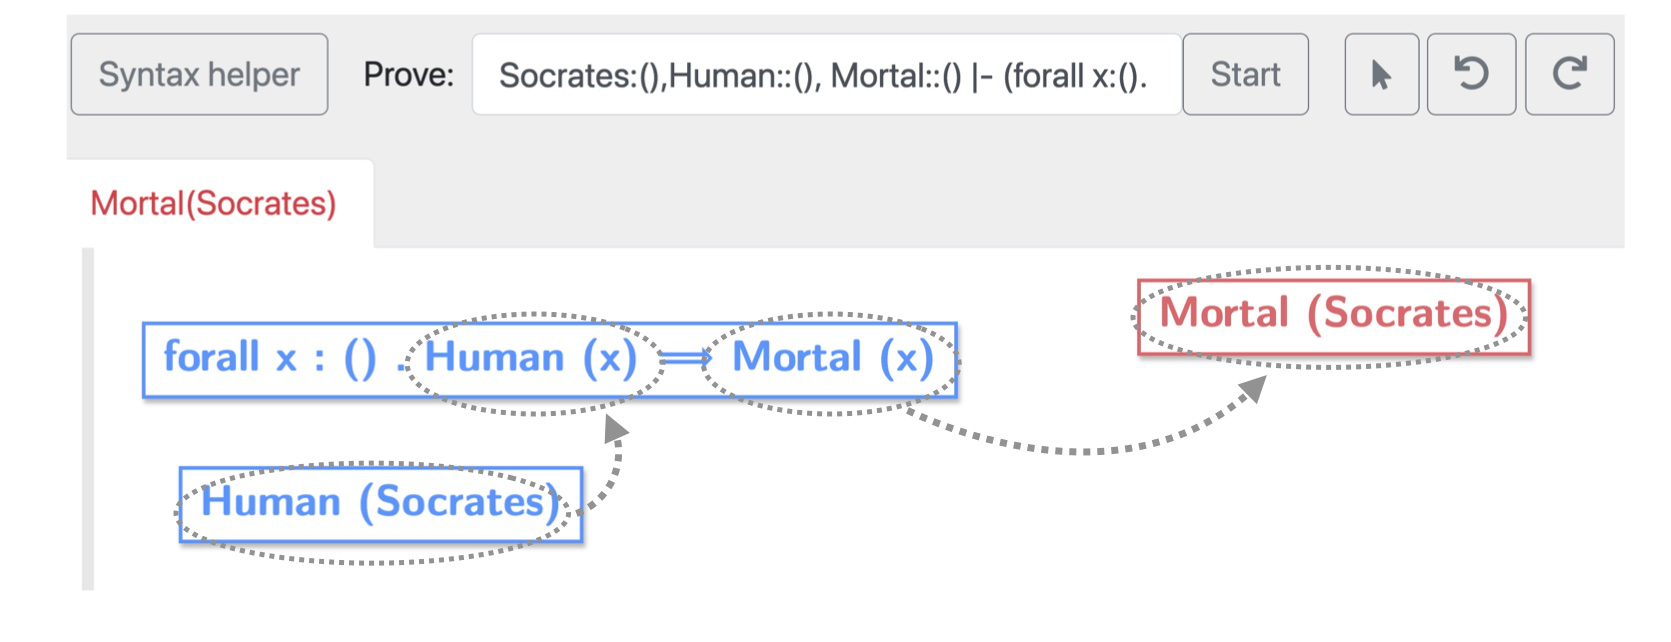
\includegraphics[width=1.3\textwidth]{actions-tag.png}}
 \end{center}
 The conclusion is red on the right, the two hypotheses blue on the left. The
 gray dotted arrows have been added to show the two possible actions.
 \caption{A partial screenshot showing a goal in the Actema prototype}
 \labfig{aristote}
 \end{figure*}

We will not consider, on paper, the details of variable renaming in
substitutions, implicitly applying the so-called Barendregt
convention, that bound and free variables are distinct and that a
variable is bound at most once.

Extending this work to simple extensions of FOL, like multi-sorted predicate
calculus is straightforward (and actually done in the Actema prototype). Some
interesting points may show up when considering how to apply this work to more
complex formalisms like type theories. We will not explore these questions here.

% Another interesting question is how our approach extends to classical logic(s),
% by using multi-conclusion sequents. In this chapter we only give a few hints on
% this topic. A more thorough investigation will be done in
% \refsec{sfl-classical}.

\section{A first example}\labsec{aristote}

\subsection{Layout}
One advantage of the PbA paradigm, is that it allows a very lean visual layout
of the proof state. There is no need to name hypotheses. In the prototype we
also dispense with a text buffer, since proofs are solely built through
graphical actions.


\reffig{aristote} shows the layout of the system using the
ancient example from Aristotle. A goal appears as a set of {\em items}
whose nature is defined by their respective colors\sidenote{We are
  well aware that, in later implementations, this color-based
  distinction ought to be complemented by some other visual
  distinction, at least for users with impaired color vision. But in
  the present description we stick to the red/blue denomination, as it
  is conveniently concise.}:
\begin{itemize}
\item A {\em red item} which is the proposition to be proved, that is the
 {\em conclusion},
\item {\em blue items}, which are the local {\em hypotheses}.
\end{itemize}

The items are what the user can act upon: either by {\em clicking} on them, or
by {\em moving} them. Each item can be positioned freely on a so-called
\emph{proof canvas}, which is depicted by the white background in
\reffig{aristote}.

Finally, note that each goal is displayed on a tab.

\subsection{Two kinds of actions}
In this example, there are two possible actions.

\begin{itemize}
\item A first one is to bring together, by drag-and-drop, the red conclusion
$\mortal(\socrates)$ with the succedant of the first hypothesis $\mortal(x)$.
This will transform the goal by changing the conclusion to $\human(\socrates)$.
\item A second possibility is to combine the two hypotheses; more precisely to
bring together the item $\human(\socrates)$ with the premise $\human(x)$ of the
first hypothesis. This will yield a new hypothesis $\mortal(\socrates)$.
\end{itemize}

The first case is what we call a {\em backward step} where the conclusion is
modified by using a hypothesis. The second case is a {\em forward step} where
two known facts are combined to deduce a new fact, that is an additional blue
item.

In both cases, the proof can then be finished invoking the logical
axiom rule. In practice this means bringing together the blue
hypothesis $\human(\socrates)$ (resp. the new blue fact
$\mortal(\socrates)$) with the identical red conclusion.


\subsection{Modelling the mechanism}

A backward step involves a hypothesis, here $\forall x.\-\human(x)
\allowbreak\limp \mortal(x)$ and the conclusion, here $\mortal(\socrates)$.
Furthermore, the action actually links together two {\em subterms} of each of
these items; this is written by squaring these subterms. The symbol ${\back}$,
used as an operator, is meant to describe the result of the interaction.
Internally, the behavior of this operator is defined by a set of rewrite rules
given in \reffig{DISL} and \reffig{DISL-U}. Here is the sequence of
rewrites corresponding to the example\sidenote{Note that $\back$ has lower
precedence than all logical connectives.}: \renewcommand{\arraystretch}{1.1}
$$\begin{array}{lll}
    &  \forall x.\human(x)\limp \select{\mortal(x)} \back \select{\mortal(\socrates)}&\\
    \step &
           \human(\socrates)\limp \select{\mortal(\socrates)}
           \back \select{\mortal(\socrates)}&
                                               \mathsf{L\forall i}\\
    \step &
           \human(\socrates)\land(\select{\mortal(\socrates)}
           \back \select{\mortal(\socrates)}) &
                                                 \mathsf{L{\limp}_2}\\
    \step &  \human(\socrates)\land \top &
                                           \mathsf{id}\\
    \step & \human(\socrates)&\mathsf{neur}\\
  \end{array}$$

Notice that:
\begin{itemize}
\item   These elementary rewrites are not visible for the user. What she sees is
  the final result of the action, that is the last expression of the rewrite
  sequence.
\item The definitions of the rewrite rules in \reffig{DISL} and
  \reffig{DISL-U} do not involve squared subterms. The information of which
  subterms are squared is only used by the system to decide which rules to
  apply in which order.
\end{itemize}

In general, the action solves the goal when the interaction ends with
the trivially true proposition $\top$. The base case being the action
corresponding to the axiom/identity rule \rnmsf{id}: $A\back A \step\top$.

A forward step, on the other hand, involves two (subterms of two)
hypotheses. The interaction operator between two hypotheses is written
$\forw$. In the example above, the detail of the interaction is:
$$
  \begin{array}{lll}
    &  \forall x .\select{\human(x)}\limp\mortal(x) \forw \select{\human(\socrates)}&\\
    \step & \select{\human(\socrates)}\limp\mortal(\socrates) \forw \select{\human(\socrates)}& \mathsf{F \forall i}\\
    \step & (\select{\human(\socrates)}\back \select{\human(\socrates)} )\limp\mortal(\socrates) &\mathsf{F{\limp}_1}\\
    \step & \top \limp\mortal(\socrates) &\mathsf{id}\\
    \step & \mortal(\socrates) & \mathsf{neul}\\
  \end{array}
$$

The final result is the new hypothesis. We come back to the study of the rewrite
rules of ${\back}$ and ${\forw}$ in \refch{sfl}.


\section{Proof steps through clicks}\labsec{clicks}
Drag-and-drop actions involve two items. Some proof steps involve only
one item; they can be associated to the action of clicking on this
item. The general scheme is that clicking on a connective or quantifier
allows to ``break'' or destruct this connective. The results of clicks
are not very surprising, but this feature is necessary to complement
drag-and-drop actions.
\begin{itemize}
\item Clicking on a blue conjunction $A\land B$ transforms the
    item into two separate blue items $A$ and $B$.
\item Clicking on a red conjunction $A\land B$ splits the goal into
    two subgoals, whose conclusions are respectively $A$ and $B$.
\item Clicking on a blue disjunction $A\lor B$ splits the goal into two subgoals
    of same conclusion, with $A$ (resp. $B$) added as a new hypothesis.
\item Clicking on the left (resp. right)-hand subterm of a red
      disjunction $A\lor B$ replaces this red conclusion by $A$
      (resp. $B$).
\item Clicking on a red implication $A\limp B$ breaks it into a
      new red conclusion $B$ and a new blue hypothesis $A$.
\item Clicking on a red universal quantifier $\forall x.A$ introduces
  a new object $x$ and the conclusion becomes $A$.
\item Clicking on a blue existential $\exists x.A$ introduces a new
  object $x$ together with a blue hypothesis $A$.
\item Clicking on a red equality $t = t$ solves the goal immediately.
\end{itemize}

One can see that these actions correspond essentially to the (right)
introduction rules of the head connective for the conclusion, and either the
elimination rule from \sys{NJ} or the left introduction rule from \sys{LJ} for
hypotheses. The exact mapping between click actions and inference rules is
given in \reftab{click-rules}. A few remarks are in order:
\begin{itemize}
  \item In the current implementation of Actema, clicking on a blue item $A
  \limp B$ will work only if the conclusion is $B$. An alternative is to use the
  {\rnmsf{{\limp}L}} rule from sequent calculus, which is applicable in every
  context.
  \item There is no action mapped to red $\bot$ items, simply because $\bot$
  does not have any introduction rule.
  \item There is currently no action mapped to blue $∀$ and red $∃$ items. The
  reason is that one needs additional information about the \emph{witness} to be
  used when instantiating with the $∀L$ or $∃R$ rule. This could be provided
  with further input (e.g. from a dialog box), but this would need a change in
  the communication protocol between the frontend and backend of Actema. Instead
  we decompose this in two steps: first the user can add the witness as a new
  object by using the \texttt{+expr} button (see \refsec{newitems}); then she
  can drag the corresponding green item and drop it on the quantified item to
  instantiate it. It is also possible to select with the mouse an arbitrary
  subexpression occurring in any item of the current goal, and then
  drag-and-drop the item holding the selected subexpression instead.
\end{itemize}

\begin{remark}[Click completeness]\label{rem:click-completeness}
  From the previous remarks and the completeness of the cut-free sequent
  calculus \sys{LJ}, it follows that click actions, when combined with new
  object declarations and DnD instantiations, provide a sufficient set of
  interactions to prove any true formula of (intuitionistic) first-order logic.
\end{remark}

\begin{table}[H]
\caption[]{Mapping of click actions to inference rules}
\labtab{click-rules}
\begin{tabular}{ccc}
	\toprule
	\thead{Head connective} & \thead{Red item} & \thead{Blue item} \\
	\midrule
  $\top$ & \rnmsf{\top R} & \rnmsf{\top L} \\
	\midrule
  $\bot$ & $\emptyset$ & \rnmsf{\bot L} \\
	\midrule
	$\land$ & \rnmsf{\land R} & \rnmsf{\land L} \\
	\midrule
	$\lor$ & \rnmsf{\lor R_1, \lor R_2} & \rnmsf{\lor L} \\
	\midrule
  $\limp$ & \rnmsf{{\limp}R} & \rnmsf{{\limp}E} \\
	\midrule
  $∀$ & \rnmsf{∀R} & $\emptyset$ \\
	\midrule
  $∃$ & $\emptyset$ & \rnmsf{∃L} \\
\end{tabular}
\end{table}


It is possible to associate some more complex effects to click actions performed
on locations deeper under connectives. This is the essence of Proof-by-Pointing,
and~\sidecite{PbP} provides ample description. Since we here focus more on
drag-and-drop actions, we do not detail further more advanced PbP features.
However we stress that these features are essentially compatible with what we
describe in this work. In fact the version of Actema presented in \refch{plugin}
provides an implementation of PbP available as a contextual menu action.


\section{Adding new items}\labsec{newitems}

Often in the course of a proof, one will want to add new items: either a new
conjecture (blue item), or a new object (green item) that would be helpful to
solve the current goal. These can be done respectively with the blue
\texttt{+hyp} and the green \texttt{+expr} buttons, which appear in the
screenshot of \reffig{edukera}. When clicked, they prompt the user
for the statement of the conjecture, or the name and expression defining the
object. The \texttt{+hyp} button will also create a new subgoal requiring to
prove the conjecture within the current context.

% This mechanism and the syntax are for now very crude. The design of
% possible smoother tools is an important issue but left for future
% work\sidenote{For instance~\cite{omar-filling-2021} deals with a
%   similar problem in the context of functional programming.}.

For now we ask the user to input textual data, in an idiosyncratic syntax
specific to the logic of Actema. A desirable, but highly non-trivial feature
would be to provide some elaborate input mechanism tailored to the type of
object the user wants to create. This would obviously require some extensibility
to new domain-specific input interfaces: typically one could imagine plugging a
tool like GeoGebra to construct geometrical figures \sidecite{gg2}, or a
categorical diagram editor like YADE\todo{add citation/link to Ambroise Lafont's
work}.

% We will not explore the design of such features in this thesis, since we focus
% on finding a universal interface for logical reasoning rather than
% domain-specific interfaces for particular types of mathematical reasoning.  Note
% however that it is a necessary feature if one wants to achieve a fully graphical
% theorem proving environment which is accessible to non-expert users.

\section{A simple example involving equality}\labsec{equality}

Most interactive theorem provers expose a \emph{rewrite} tactic that allows the
use of equality hypotheses, that is known equations of the form $t = u$, in
order to replace some occurrences of $t$ by $u$ (or symmetrically, occurrences
of $u$ by $t$). This substitution can be performed in the conclusion or in
hypotheses. Specifying the occurrences to be replaced with textual commands can
be quite tedious, since it involves either dealing with some form of
naming/numbering to designate locations of subterms, or writing manually
patterns which duplicate parts of the structure of terms.

\begin{figure*}
  \begin{center}
    \fbox{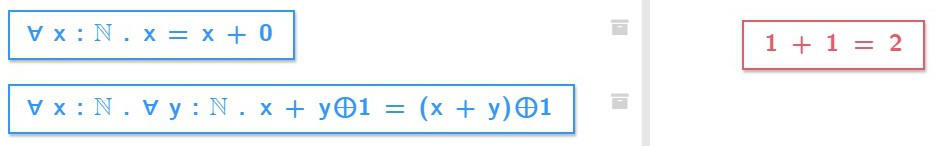
\includegraphics[width=1.3\textwidth]{oneplusone.png}}
  \end{center}
  \caption{Proving $1 + 1 = 2$ in Peano arithmetic}
  \labfig{oneplusone}
\end{figure*}

In our setting we can provide this replacement operation through
drag-and-drop. The user points at the occurrence(s) of $t$ to be
replaced, and then brings them to the corresponding side of the
equality.

\reffig{oneplusone} shows a very elementary example where one wants to prove
$1+1=2$ in the setting of Peano arithmetic. For any number $n$, we write
$\suc{n}$ to denote the application of the successor function to $n$; closed
terms are directly written in decimal notation. The proof goes as follows:
\begin{itemize}
  \item We link the left-hand side $x + \suc{y}$ of the second addition axiom with $1 + 1$ in the conclusion, which has the effect of rewriting $1 + 1$ into $\suc{(1 + 0)}$:
    $$
      \begin{array}{lll}
        & \forall x. \forall y. \select{x + \suc{y}} = \suc{(x + y)} \back \select{1 + 1} = 2 & \\
        \step & \forall y. \select{1 + \suc{y}} = \suc{(1 + y)} \back \select{1 + 1} = 2 &\mathsf{L\forall i} \\
        \step & \select{1 + \suc{0}} = \suc{(1 + 0)} \back \select{1 + 1} = 2 &\mathsf{L\forall i} \\
        \syneq & \select{1 + 1} = \suc{(1 + 0)} \back \select{1 + 1} = 2 & \\
        \step & \suc{(1 + 0)} = 2 &\mathsf{L{=}_1}
      \end{array}
    $$
  \item We link the right-hand side $x + 0$ of the first addition axiom with $1 + 0$ in the conclusion, which rewrites $1 + 0$ into $1$:
    $$
      \begin{array}{lll}
        & \forall x. x = \select{x + 0} \back \suc{(\select{1 + 0})} = 2 & \\
        \step & 1 = \select{1 + 0} \back \suc{(\select{1 + 0})} = 2 &\mathsf{L\forall i} \\
        \step & \suc{1} = 2 &\mathsf{L{=}_2} \\
        \syneq & 2 = 2 &
      \end{array}
    $$
\end{itemize}

We end up with the conclusion $2 = 2$, which is provable by a simple click.
Notice how the orientation of the two rewritings is determined by which side of
the equality is selected. Also, in this case, the rewritings
correspond to backward proof steps, because the rewriting is performed
in the conclusion. Similar rules (\rnmsf{F{=}_1} and \rnmsf{F{=}_2}) are
used to perform rewritings in hypotheses.


\section{Drag-and-dropping through connectives}\labsec{dnd-examples}
We mentioned in \refsec{clicks} that it is possible to destruct logical
connectives through click actions. In many cases however, this will not be
necessary: because a drag-and-drop involves subterms of the items involved, one
can often directly use (resp. act on) the part of the hypothesis (resp.
conclusion) which is of interest.

\subsection{Conjunction and disjunction}
The conjunction is an easy to explain case. A hypothesis of the form
$A\land B$ can be used directly both as evidence for $A$ and as evidence
for $B$. This is modeled by the rules \rnmsf{L\land_1} and
\rnmsf{L\land_2}. A very simple action is thus:
$$
\begin{array}{llll}
  \select{A}\land B \back \select{A} & \step& \select{A} \back
  \select{A} \hbox to 1cm {\hfil}&\mathsf{L \land_1}\\
                                       & \step &\top & \mathsf{id}
\end{array}
$$

On the other hand, considering a conjunctive goal $A\land B$, one can
simplify or solve one of the branches by a DnD action. This involves
rules \rnmsf{R \land_1} and
\rnmsf{R \land_2}. For instance:
$$
\begin{array}{llll}
  \select{A} \back \select{A}\land B &
                                         \step& (\select{A} \back
                                         \select{A})\land B &\mathsf{R \land_1}\\
                                       & \step& \top \land B  & \mathsf{id}\\
  &\step& B&\mathsf{neul}
\end{array}
$$

Red disjunctions work similarly to conjunctive goals, except that solving one
branch will solve the entire goal. A nice consequence of this, which is hard to
simulate with textual tactics, is that one can just simplify one branch of a
disjunction without comitting to proving it entirely:
$$
\begin{array}{llll}
  \select{A} \back (B \land \select{A}) \lor C
    & \step & (\select{A} \back B \land \select{A}) \lor C &\mathsf{R\lor_1}\\
    & \step & (B \land (\select{A} \back \select{A})) \lor C &\mathsf{R\land_2}\\
    & \step & (B \land \top) \lor C &\mathsf{id}\\
    & \step & B \lor C &\mathsf{neur}
\end{array}
$$

Disjunctive hypotheses also have a backward behavior defined by the rules
\rnmsf{L\lor_1} and \rnmsf{L\lor_2}, although in most cases one will prefer the
usual subgoal semantics associated with click actions. More interesting is
their forward behavior with the rules \rnmsf{F\lor_1} and \rnmsf{F\lor_2}, in
particular when they interact with negated hypotheses. For instance:
$$
\begin{array}{llll}
  \select{A} \lor B \forw \neg \select{A}
    & \step & (\select{A} \forw \neg\select{A}) \lor B &\mathsf{F\lor_1}\\
    & \step & \neg (\select{A} \back \select{A}) \lor B &\mathsf{F{\limp}_1}\\
    & \step & \neg \top \lor B &\mathsf{id}\\
    & \step & \bot \lor B &\mathsf{neul}\\
    & \step & B &\mathsf{neul}\\
\end{array}
$$

We have noticed that on some examples, such actions could provide a
significant speed-up with respect to traditional textual command
provers. We give a more concrete example in \refsec{edukera}.

Notice that we used rules associated with implication, since negation can be
defined by $\neg A \defeq A \limp \bot$.

\subsection{Implication}\labsec{implication}
The implication connective is crucial, because it is not monotone. More
precisely, the roles of hypotheses and conclusions are reversed on the
left of an implication. We start with some very basic examples
for the various elementary cases.

Using the right hand part of a hypothesis $A\limp B$ turns a 
conclusion $B$ into $A$. 
$$
\begin{array}{llll}
  A\limp \select{B} \back \select{B} &\step& A\land (\select{B}
                                                \back
                                                \select{B})&\mathsf{L
                                                             {\limp}_2}\\
                                         &\step&A\land\top & \mathsf{id}\\
    &\step& A&\mathsf{neul}
\end{array}
$$

This can also be done under conjunctions and/or disjunctions:
$$
  A\limp \select{B} \back C \land (D\lor \select{B}) ~~ \steps ~~ C \land (D\lor A)
$$

An interesting point is what happens when using implications with
several premisses. The curried and uncurried versions of the
implication will behave exactly the same way:

$$
  A\limp B \limp \select{C} \back D\lor \select{C}
  ~~~\/ ~\steps~~~  D\lor (A\land B)
$$
and:
$$
  A\land B \limp \select{C} \back D\lor \select{C}
  ~~~ \/ ~\steps~~~  D\lor (A\land B)
$$


As we have seen in Aristotle's example (\refsec{aristote}), blue
implications can also be used in forward steps, where another
hypothesis matches one of their premisses.

A first nice feature is the ability to strengthen a hypothesis by
providing evidence for any of its premises:
$$
B\limp \select{A}\limp C \forw \select {A}  ~~\/~\/~\steps~\/~~~~~
B\limp C$$
and again the same can be done for the uncurryfied version:
$$
B\land \select{A}\limp C \forw \select {A}  ~\/~\/~\steps~\/~~~~~
B\limp C.$$

The two aspects of the implication can be combined:

$$
B\limp \select{A}\limp C \forw D\limp\select {A}  ~\/~\/~\steps~\/~~~~~
B\limp D\limp C$$
or:
$$
B\land \select{A}\limp C \forw D\limp\select {A}  ~\/~\/~\steps~\/~~~~~
B\land D \limp C.$$


Note that there is almost no difference in the way one uses different
versions of a hypothesis $A\limp B\limp C$, $A\land B\limp
C$, but also $B\limp A\limp C$, in forward as well as in
backward steps\sidenote{When viewed as types through the Curry-Howard
isomorphism, $A\limp B\limp C$, $A\land B\limp C$, $B\land
A\limp C$ and $B\limp A\limp C$ are {\em isomorphic types};
and Roberto di Cosmo~\cite{ISOSBook} has also precisely underlined
that type isomorphisms should help to free the programmer from
arbitrary syntactical choices.}. This underlines, we hope, that our
proposal makes the proof construction process much less dependent on
arbitrary syntactical details, like the order of hypotheses or whether
they come in curryfied form or not.

Also, the rules for implication combined with the rules for equality
\rnmsf{L{=}_i} or \rnmsf{F{=}_i} naturally give access to {\em
  conditional rewriting}; we detail this in combination with
quantifiers in the next section.

%A powerful property of our rewrite rules is that this behavior is true at
%\emph{any depth} under logical connectives.


As for red implications, they also have a backward semantics with the rules
\rnmsf{R{\limp}_1} and \rnmsf{R{\limp}_2}, but most of the time one
will want to destruct them immediately by click. An exception could be if one
wants to simplify some part of an implicative, inductive goal before starting
the induction.

\subsection{Quantifiers}
As the first example of this chapter shows, drag-and-drop actions work through
quantifiers and can trigger instantiations of quantified variables. This is made
possible by the rules \rnmsf{L\forall i} and \rnmsf{F\forall i}, which allow the
instantiation of a variable universally quantified in a hypothesis.

Symmetrically, a variable quantified existentially in a conclusion can
also be instantiated. For instance:

$$\begin{array}{llll}
    \select{A(t)}\back \exists x.\select{A(x)}&\step&
                                                      \select{A(t)}\back\select{A(t)}&\mathsf{L}\forall\mathsf{i}
    \\
                                               &\step& \top&\mathsf{id}
  \end{array}
  $$

An interesting feature is the possibility to modify propositions under
quantifiers. Consider the following possible goal:
% Take this example involving equality:
% $$\begin{array}{clc}
%    & \forall x.\select{ x+0 = x }\back \forall a. \select{a+0} = 0 +
%      a&  \\
%          \step&\forall a.(\forall x.\select{x+0 = x }\back \select{a+0} =
%             0 +a)&\mathsf{R}\forall\mathsf{s}\\
%      \step&\forall a. (\select{a+0=a}\back  \select{a+0} = 0 +a)& \mathsf{L}\forall\mathsf{i}\\
%      \step&\forall a. a = 0+a&\mathsf{L}=1
%                                \end{array}$$
% Performing such a transformation of the goal $\forall a.a+0=0+a$
% without destroying the head quantifier is not trivial traditional
% provers; here it is done through one simple action.
$$\forall a.\exists b. A(f(a)+g(b))$$
where $A$, $f$ and $g$ can be complex expressions. Suppose we have a
lemma allowing us to prove:
$$\forall a.\exists b. A(g(b)+ f(a)).$$
Switching from one formulation to the other, involves one use of the
commutativity property $\forall x.\forall y. x+y=y+x$.
% But because this has to be performed under two quantifiers, doing this in
% traditional interactive theorem provers can be tedious. For instance in Coq, one
% must use a specific tactic called \texttt{setoid_rewrite}.
In our setting, the equality can be used under quantifiers in one single action:
$$
\begin{array}{ll}
  &\forall x.\forall y. \select{x+y}=y+x \back \forall a.\exists b. A(\select{f(a)+g(b)})\\
\steps & \forall a.\exists b. A(g(b)+f(a))
\end{array}$$


Note also that it is possible to instantiate only some of the universally
quantified variables in the items involved. In general, a universally
quantified variable can be instantiated when the quantifier is in a
negative position; for instance:
%\setlength{\abovedisplayskip}{-5pt}
%\setlength{\belowdisplayskip}{0pt}
%\setlength{\belowdisplayshortskip}{0pt}
$$
\begin{array}{rcl}
 \forall x.\forall
 y. \select{P(y)}\limp R(x,y)\forw \select{P(a)} ~\/~\steps
~\/~ \forall x. R(x,a)
 %% \\
 %% \mbox{\hbox to 0pt{\hss or equivalently:}}
 %% \forall y.\forall
 %% x. \select{P(x)}\limp R(x,y)\forw \select{P(a)} \steps
 %% \forall y. R(a,y)
\end{array}
$$
This last example illustrates how partial instantiation abstracts away the order
in which quantifiers are declared, very much like the partial application
presented earlier for implication\sidenote{This fact should not be too
surprising to the reader familiar with dependent type theory, where implication
is usually defined as a special case of universal quantification.}.
%% What the last example stresses is, again, that syntactical details,
%% here the order in which variables are quantified, are much less
%% relevant in the gestual proof constructions than in their textual
%% counterparts.


Again, in some cases, only some existential quantifiers may be
instantiated following a linkage:
$$
\begin{array}{rcl}
\select{P(a)}\back \exists x.\exists y. \select{P(y)}\land R(x,y)
 ~\/~\steps
~\/~
    \exists x. R(x,a)
\end{array}
$$

When using an existential assumption, one can either destruct it
through a click, or use or transform it through a DnD; for instance:
$$
\exists x.\select{P(x)}\forw \forall y.\select{P(y)}\limp
Q(y)  ~\/~\steps
~\/~\exists x.Q(x)
$$

\subsection{Dependency between variables}\labsec{acyclicity}
Some more advanced examples yield simultaneous instantiations of
existentially and universally quantified variables. In such cases, the
system needs to check some dependency conditions. For instance, the
following linkage is valid and solves the goal through one action:
$$
\begin{array}{lll}
  &\exists y. \forall x. \select{R(x,y)}\back \forall x'.\exists
    y'. \select{R(x',y')}& \\
  \step& \forall y.(\forall x. \select{R(x,y)}\back \forall x'.\exists
        y'. \select{R(x',y')} ) \mbox{\hbox to 12pt{\hfill}}& \mathsf{L}\exists\mathsf{s}\\
  \step &\forall y. \forall x'. (\forall x. \select{R(x,y)}\back \exists
  y'. \select{R(x',y')} ) ~~~~~~~~~~~~&\mathsf{R}\forall\mathsf{s}\\
  \step &  \forall y. \forall x'. (\forall
         x. \select{R(x,y)}\back\select{R(x',y)} )&\mathsf{R}\exists\mathsf{i}\\
  \step&   \forall y. \forall
           x'. (\select{R(x',y)}\back\select{R(x',y)} )&\mathsf{L}\forall\mathsf{i}\\
   \step  &  \forall y. \forall
           x'. \top & \mathsf{id}\\
\steps& \top
\end{array}
$$

But the converse situation is not provable; the system will refuse
the following linkage:
$$
\begin{array}{rcl}
  \forall x. \exists y. \select{R(x,y)}\back \exists y'.\forall x'. \select{R(x',y')}
\end{array}
$$
Indeed, there is no reduction path starting from this linkage ending with the
\textsf{id} rule. This can be detected by the system because the unification of
$R(x,y)$ and $R(x',y')$ here results in a cycle in the instantiations of
variables\sidenote{We will come back to this in \refsec{linkages}. Also notice
that this example requires to use full (first-order) unification, not only
matching.}. The system thus refuses this action.

\subsection{Conditional rewriting}
The example given in \refsec{equality}, although very simple,
already combines the rules for equality and for quantifiers. When also
using implication, one obtains naturally some form of conditional
rewriting. To take another simple example, suppose we have a
hypothesis of the form:
$$\forall x. x\neq 0 \limp f(x) = g(x)$$

We can use this hypothesis for replacing a subterm $f(t)$ by $g(t)$,
which will generate a side-condition $t\neq 0$:
$$
\begin{array}{lll}
  &\forall x. x\neq 0 \limp \select{f(x)} = g(x) \back A(\select{f(t)}) &\\
  \step & t\neq 0 \limp \select{f(t)} = g(t) \back A(\select{f(t)}) &\mathsf{L \forall i}\\
  \step & t\neq 0 \land (\select{f(t)} = g(t) \back A(\select{f(t)})) & \mathsf{L{\limp}_2}\\
  \step &  t\neq 0 \land A(g(t)) &\mathsf{L{=}_1} \\
\end{array}$$

One could similarly do such a rewrite in a hypothesis. Furthermore,
the conditional rewrite can also be performed under quantifiers; for instance:
$$
\begin{array}{lll}
  &\forall x. x\neq 0 \limp \select{f(x)} = g(x) \back \exists y . A(\select{f(y)})
  &\mathsf{R \exists s}\\
  \step &\exists y. ( \forall x. x\neq 0 \limp \select{f(x)} = g(x) \back A(\select{f(y)})) &\mathsf{L \forall i}\\
  \step & \exists y. ( y\neq 0 \land ( \select{f(y)} = g(y) \back A(\select{f(y)}) )) &\mathsf{L{\limp}_2} \\
  \step & \exists y .( y\neq 0 \land A(g(t))) &\mathsf{L{=}_1} \\
\end{array}$$


% \todo{Remove page break (while keeping the wide page layout for the rules).}

\pagelayout{wide} % No margins
\begin{figure}
  \fontsize{10}{10.5}\selectfont
    \renewcommand{\arraystretch}{1.25}
  \begin{framed}
  \begin{mathpar}
    \begin{array}{r@{\quad}c@{\quad}lr}
        \multicolumn{4}{c}{\textsc{Backward}} \\[2em]

        {A \back A}&\step&\top &\mathsf{id}\\
        {t = u \back \subst{A}{t}{x}}&\step&\subst{A}{u}{x} &\mathsf{L{=}_1}\\
        {t = u \back \subst{A}{u}{x}}&\step&\subst{A}{t}{x} &\mathsf{L{=}_2}\\[1em]

        {(B \land C) \back A}&\step&        {B \back A}&\mathsf{L \land_1}\\
        {(C \land B) \back A}&\step&        {B \back A}&\mathsf{L \land_2}\\
        {A \back~(B \land C)}&\step&        {(A \back B) \land C}&\mathsf{R \land_1}\\
        {A \back~(C \land B)}&\step&        {C \land (A \back B)}&\mathsf{R \land_2}\\[1em]
        
        {(B \lor C) \back A}&\step&        {(B \back A) \land (C \limp A)}&\mathsf{L \lor_1}\rever\\
        {(C \lor B) \back A}&\step&        {(C \limp A) \land (B \back A)}&\mathsf{L \lor_2}\rever\\
        {A \back~(B \lor C)}&\step&        {(A \back B) \lor C}&\mathsf{R \lor_1}\\
        {A \back~(C \lor B)}&\step&        {C \lor (A \back B)}&\mathsf{R \lor_2}\\[1em]

        {(C \limp B) \back A}&\step&        {C \land (B \back A)}&\mathsf{L{\limp}_2}\\
        {A \back~(B \limp C)}&\step&        {(A \forw B) \limp C}&\mathsf{R{\limp}_1}\rever\\
        {A \back~(C \limp B)}&\step&        {C \limp (A \back B)}&\mathsf{R{\limp}_2}\rever\\[1em]

        % {A \back \neg B}&\step&        {\neg (A \forw B)}&\mathsf{R\neg}\rever\\[1em]

        {(\forall x. B) \back A}&\step&        {\subst{B}{x}{t} \back A}&\mathsf{L \forall i}\\
        {(\forall x. B) \back A}&\step&        {\exists x. (B \back A)}&\mathsf{L \forall s}\\
        {A \back~(\forall x. B)}&\step&        {\forall x. (A \back B)}&\mathsf{R \forall s}\rever\\[1em]

        {(\exists x. B) \back A}&\step&        {\forall x. (B \back A)}&\mathsf{L \exists s}\rever\\
        {A \back~(\exists x. B)}&\step&        {A \back \subst{B}{x}{t}}&\mathsf{R \exists i}\\
        {A \back~(\exists x. B)}&\step&        {\exists x. (A \back B)}&\mathsf{R \exists s}\\
    \end{array}
  % \end{mathpar}
  \and
  % \textsc{Forward}\\
  % \begin{mathpar}
    \begin{array}{r@{\quad}c@{\quad}lr}
      \multicolumn{4}{c}{\textsc{Forward}} \\[2em]

      % \R[\mathsf{lnn}]
      %   {\ifill{\eta}{\efill{A}{A} \forw \efill{B}{B}}}
      %   {\ifill{\eta}{\ifill{A}{A} \land \ifill{B}{B}}}
      % \\
      {\subst{A}{t}{x} \forw~(t = u)} &\step& {\subst{A}{u}{x}}&\mathsf{F{=}_1}\\
      {\subst{A}{u}{x} \forw~(t = u)} &\step& {\subst{A}{t}{x}}&\mathsf{F{=}_2}\\[1em]

        {A \forw~(B \land C)} &\step&   {A \forw B}&\mathsf{F\land_1}\\
        {A \forw~(C \land B)}&\step&        {A \forw B}&
            \mathsf{F \land_2}\\[1em]

        {A \forw~(B \lor C)}& \step&       {(A \forw B) \lor C}
      &
      \mathsf{F \lor_1}\\
        {A \forw~(C \lor B)}&\step&        {C \lor (A \forw B)}&
            \mathsf{F \lor_2}\\[1em]

        {A \forw~(B \limp C)}
&\step&        {(A \back B) \limp C}
      &\mathsf{F{\limp}_1}\\
        {A \forw~(C \limp B)}&\step&        {C \limp (A \forw B)}&
            \mathsf{F{\limp}_2}\\[1em]

%         {A \forw \neg B}
% &\step&        {\neg (A \back B)}
%       &\mathsf{F\neg}\\[1em]

        {A \forw~(\forall x. B)}
&\step&        {A \forw \subst{B}{x}{t}}
      &
      \mathsf{F \forall i}\\
        {A \forw~(\forall x. B)}&\step&        {\forall x. (A \forw B)}&
            \mathsf{F \forall s}\\[1em]

              {A \forw~(\exists x. B)}&\step&{\exists x. (A \forw B)}&
              \mathsf{F \exists s}\rever\\[1em]
              
          {B \forw A}&\step&
          {A \forw B}& \mathsf{Fcomm}\\
    \end{array}
    \end{mathpar}
    ~\\[1em]
    In the rules $\{\mathsf{L \forall s}, \mathsf{L \exists s}, \mathsf{R \forall
    s}, \mathsf{R \exists s}, \mathsf{F \forall s}, \mathsf{F \exists s}\}$, $x$
    is not free in $A$.
  \end{framed}
  \caption{Linking rules}
  \labfig{DISL}
\end{figure}

\begin{figure}
  \fontsize{10}{10.5}\selectfont
  \begin{framed}
  {\textsc{Units}}\\
  \begin{mathpar}
    \renewcommand{\arraystretch}{1.2}
    \begin{array}{lr@{\quad}c@{\quad}lc}
   \pair{\mcirc}{\dagger} \in \{
      \pair{\land}{\top},
      \pair{\lor}{\bot},
      \pair{\limp}{\top}
      \}&
      {\dagger \mcirc A}&\step&A&\mathsf{neul}\\
 \pair{\mcirc}{\dagger} \in \{
      \pair{\land}{\top},
      \pair{\lor}{\bot}
      \}&
      {A \mcirc \dagger}&\step&A&\mathsf{neur}\\
   \pair{\mcirc}{\dagger} \in \{
      \pair{\land}{\bot},
      \pair{\lor}{\top}
      \}&
      {\dagger \mcirc A}&\step&\dagger&
       \mathsf{absl}\\
  \pair{\mcirc}{\dagger} \in \{
      \pair{\land}{\bot},
      \pair{\lor}{\top},
      \pair{\limp}{\top}
      \}&
      {A \mcirc \dagger}
      &\step&\dagger& \mathsf{absr}\\
  \pair{\mdiam}{\dagger} \in \{
    \pair{\forall}{\top},
    \pair{\exists}{\bot}
    \}&      {\mdiam x. \dagger}&\step&\dagger&    \mathsf{absq}
    \\
&      {\bot \limp A}&\step&\top&\mathsf{efq} 
      \end{array}
  \end{mathpar}
  \end{framed}
  % \begin{framed}
  % {\sc Resources}
  % \begin{mathpar}
  %   %\R[\mathsf{conp}]
  %   %  {\pi\{A \lor A\}}
  %   %  {\pi\{A\}}
  %   %\and
  %   \R[\mathsf{conn}]
  %     {\ifill{\eta}{A \land A}}
  %     {\ifill{\eta}{A}}
  %   \and
  %   \R[\mathsf{wkn}]
  %     {\ifill{\eta}{\top}}
  %     {\ifill{\eta}{A}}
  % \end{mathpar}
  % \end{framed}
  \caption{Unit elimination rules}
  \labfig{DISL-U}
\end{figure}
\pagelayout{margin} % Restore margins

\section{Related works}\labsec{pba-rw}

\paragraph{Window inference}

We have already mentioned Proof-by-Pointing, which was part of the CtCoq and
Pcoq efforts \sidecite{amerkad-mathematics-2001} to design a graphical user
interface for the Coq proof assistant. Another contemporary line of work was the
one based on \emph{window inference}, also mentioned in \refsec{intro-rw}. In
\sidecite{robinson-formalizing-1993}, window inference is described as a general
proof-theoretical framework, which aims to accomodate for the pervasive use of
\emph{equivalence transformations} throughout mathematics and computer science.

% In \cite{robinson-formalizing-1993}, they describe it as a new kind
% of proof-theoretic framework, which aims to accomodate for the pervasive use of
% \emph{equivalence transformations} throughout mathematics and computer science.
% For this purpose, it provides facilities for describing how to focus on specific
% subexpressions, and perform transformations on them that preserve a given
% equivalence relation, while keeping and exploiting information from the context
% where they occur. It is noted in \cite{grundy-window-1991} that the framework
% can be extended to more general relations like preorders, which might typically
% be used to capture the entailment relation of a logic.
Window inference has been used both for general-purpose logics like HOL
\sidecite{grundy-window-1991}, and in more specialized settings like program
refinement \sidecite{grundy-window-1992}. It naturally lends itself to
integration in a graphical user interface (\sidecite{langbacka-tkwinhol-1995},
\sidecite{goos-tas-2000}), where the user can \emph{focus} on a subexpression by
clicking on it. One is then presented with a new \emph{graphical} window,
holding the selected expression as well as an extended set of hypotheses
exposing information inferrable from the context of the expression. The user can
pick from a list of valid transformations to be applied to the expression,
before closing the window. This propagates the transformations to the parent
window by replacing the old subexpression by the new one, without modifying the
surrounding context.

This process is quite reminiscent of the rewriting produced by our DnD
actions. One key difference is that window inference rules can be
applied stepwise, while we choose to hide the sequence of rules that
justifies a DnD. The window inference approach gives to the user a
precise control of the transformations to be performed and thus could
inspire interesting extensions of our work.

% This is because
% DnD actions embody the specific intent of justifying an \emph{expression} by
% another \emph{user-specified} expression, which is either assumed to be, or
% trivially equivalent. In contrast, window inference is about justifying the
% \emph{equivalence} of an expression to another, \emph{not yet specified}
% expression. Another way to see it is that our ``link inference'' technique aims
% to capture the process of \emph{applying} some knowledge, while window inference
% provides an interface for the \emph{construction} of new knowledge. They thus
% appear as equally valid and even complementary approaches, that could benefit
% from being implemented in the same interface.


\paragraph{Other gestural proof systems}

There are other proof systems which include drag-and-drop features. Two of them
are the KeY Prover \sidecite{ahrendt-using-2016} and TAS
\sidecite{goos-tas-2000}. TAS is a window inference system tailored for program
refinement, and uses DnD actions between an expression and a transformation, in
order to apply the latter to the former.
%This is obviously different from our use of DnD between entities
%of the same kind, and can be explained by the comparison made in the previous
%paragraph.
As for the KeY Prover, its usage of DnD overlaps only a very small
portion of usecases that we hinted at in \refsec{edukera}, namely
the instantiation of quantifiers with objects.

We can also mention the recent work of Zhan et al. \sidecite{zhan-design-2019}.
They share with us the vision of a proof assistant mainly driven by gestural
actions, which requires far less textual inputs from the user. However, they
only consider point-and-click actions, and rely on a text-heavy presentation at
two levels:
\begin{enumerate}
  \item the proof state, which is a structured proof text in the style of
  Isar~\sidecite{isar};
  \item the proof commands, which can only be performed through choices in
  textual menus.
\end{enumerate}

% The latter can be useful to integrate specific actions which do not fit
% naturally in the gestural paradigm. But because basic reasoning with logical
% connectives and equations occurs so often in virtually any proof, we believe it
% deserves a special treatment in the interface, and our work shows that
% drag-and-drop gestures can be used efficiently for that purpose. This was
% already a concern in \cite{amerkad-mathematics-2001}, where PbP is seen as a
% mean to \emph{``increase the bandwidth between the user and the logical
% engine''}, along with other devices like advanced graphical notations. The
% authors also described how PbP is partially compatible with the production
% \emph{in real time} of a proof text in quasi-natural language, thus close to an
% Isar proof. We conjecture that our drag-and-drop mechanism also has this
% capability, and in fact solves some of the problems induced by the limitation of
% PbP to a single selection.


\paragraph{Explicit proof objects}

Finally let us mention various recent implementations proposing various ways to
construct proofs graphically: Building Blocks~\sidecite{buildingblocks}, the
Incredible Proof Machine~\sidecite{blanchette-visual-2016},
Logitext\sidenote{\url{http://logitext.mit.edu/main}} and Click \&
coLLecT~\cite{clickcollect}. In particular, Logitext and Click \& coLLecT
exploit the same idea of associating click actions on head connectives to
inference rules in sequent calculus. But these systems focus more on explicating
the proof object than on making its construction easier.
\setchapterpreamble[u]{\margintoc}
\chapter{Subformula Linking}
\labch{sfl}

In this chapter, we engage in a thorough analysis of the logical semantics of
DnD actions, which were introduced informally through examples in \refch{pba}.
We do this mainly from the formal perspective of deep inference proof theory,
following the original work of K. Chaudhuri on his \emph{subformula linking}
paradigm \cite{Chaudhuri2013}. But we always keep in mind the intended
application to proof assistants, by motivating various design choices --- actual
or prospective --- as ways to improve the UX of interactive proof building.

The chapter is organized as follows: \refsec{linkages} introduces the notions of
context and polarity, and explains how DnD actions are specified by the user
interactively through schemas called \emph{linkages}. \refsec{validity} explains
how one can identify a subset of linkages that guarantees a \emph{productivity}
property on DnD actions. \refsec{action} describes the overall structure of how
linkages translate into logical steps, and \refsec{invert} discusses some
subtleties of this translation that are related to the concept of
\emph{focusing} in automated proof search. \refsec{soundness} shows that the
logical steps are sound, and \refsec{productivity} states and proves formally
the productivity property. Finally, \refsec{dnd-completeness} shows how DnD
actions can be turned into a complete deductive system without any need for
click actions.

\section{Linkages}\labsec{linkages}

Like most rewriting systems on terms (that is, tree-shaped data), the rewrite
rules of \reffig{DISL} and \reffig{DISL-U} apply at any depth inside formulas.
However logically, the shape of the \emph{context} in which this rewriting
occurs can provide important information, either to ensure soundness of the
performed transformation (\refsec{soundness}, \refsec{dnd-completeness}), or 
to understand the status of quantified variables (\refsec{identity}).

As is standard in term rewriting, our notion of context will correspond to that
of a (formula) tree with a distinguished leaf called its \emph{hole}.
% \sidenote{More precisely, our contexts correspond to what is called a
% ``structure'' in the first deep inference formalism to date, the \emph{Calculus
% of Structures} (see \refsec{cos}).}

\begin{definition}[Formula context]\label{def:formula-context}
  A \emph{formula context}, written $A\hole$, is a proposition containing
  exactly one occurrence of a specific propositional variable $\hole$ which is
  not used elsewhere.

  Given another proposition $B$, we write $A\select{B}$ for the
  proposition obtained by replacing $\hole$ in $A\hole$ by $B$. Note
  that this replacement is not a substitution because it allows variable
  capture. For instance $\forall x.\select{P(x)}$ is the proposition
  $\forall x.P(x)$.
\end{definition}

\begin{definition}[Path]\label{def:path}
A path is a proposition where one subformula has been
selected. Formally, a path is a pair $(A\hole, B)$ formed by one
context and one proposition:
\begin{itemize}
\item $A\hole$ is called the {\em context} of the path,
\item $B$ is called the {\em selection} of the path.
\end{itemize}

The path $(A\hole, B)$ can be viewed as the proposition
$A\select{B}$.  For readability, we will generally also write
$A\select{B}$ for the path $(A\hole, B)$.
\end{definition}

\begin{definition}[Inversions]
  Given a context $A\hole$, the number of inversions in $A\hole$,
  written $\inv(A\hole)$, is the number of subterms of $A\hole$
  which are of the form $C\hole\limp D$; that is the number of
  times the hole is on the left-hand side of an implication.
  \end{definition}
\noindent  For instance:
  $$
\begin{array}{rcl}
    \inv(D\land \hole)&=& 0\\
    \inv((D\land \hole)\limp E)&=&1\\
    \inv((\hole\limp C)\limp D) &=& 2
\end{array}
$$

\begin{definition}[Polarity of a context]\label{def:polarity}
We will write $A^+\hole$ to specify that a context is {\em positive},
meaning that $\inv(A^+\hole)$ is even. Symmetrically, $A^-\hole$ will be
used for {\em negative} contexts, meaning that $\inv(A^-\hole)$ is odd.
\end{definition}

% In demonstrating soundness, we focused solely on the two \emph{items} involved
% in a DnD action. But

In addition to the items involved, every DnD action specifies the
\emph{selection} of a subterm in each item, which can be expressed formally as a
path (Definition \ref{def:path}). We call \emph{linkage} the combined data of
the two items together with the selection, since the intent is to \emph{link}
the subterms to make them interact in some way.

\begin{remark}
In this thesis we only consider linkages between two subterms, but as noted in
\refsec{equality}, rewriting is an example of action that can benefit from
allowing multiple selections\sidenote{A restricted kind of multi-occurrence
rewrite is already available in the standalone version of Actema: one needs to
enter \emph{selection mode}, by either toggling the dedicated button (the one
with the mouse cursor in \reffig{aristote}), or holding down the \texttt{shift}
key. Then one can click successively on all occurrences of a term $t$ that are
to be rewritten, in order to add them to the selection. To perform the rewriting
to some other term $u$, the last step is to drag an equality hypothesis $t = u$
(or $u = t$) and drop it on any item holding one of the selected occurrences of
$t$.}.
\end{remark}

Each kind of DnD action is mapped in the system to a specific form of linkage,
which is designed to hold all the information necessary for the correct
execution of the action. In this way the system can automatically search for
linkages of a certain form, and propose to the user all well-defined actions
associated to these linkages.

\begin{remark}
  In the future, one can imagine several DnD actions associated to a given
  linkage. In this case, the user could be queried to choose the action to be
  performed (typically with a pop-up menu). However with the actions considered
  in this thesis, such ambiguities never arise.
\end{remark}

On the ``items axis'', we already distinguished between backward and forward
linkages, written respectively $A \back B$ and $A \forw B$. If the items are
unspecified, we will write $A \link B$.

Using the ``selection axis'', we can specify a further distinction that was
informal up to now: that of \emph{logical} action and \emph{rewrite} action.
\begin{itemize}
  \item \emph{Logical} linkages link two subformulas. Thus they have the form
  $B\select{A} \link C\select{A'}$.
  \item \emph{Rewrite} linkages link one side of an equality with a first-order
  term. Using liberally the notations from Definitions \ref{def:formula-context} and
  \ref{def:path}, they thus have the form
  $$B\select{\select{t} = u} \link C
  \select{t'} \text{\ (or symmetrically $B\select{u = \select{t}} \link C
  \select{t'}$)}$$
  % \item \emph{Instanciation} actions correspond to specialization of universal
  % hypotheses, and witness choice for existential goals.
\end{itemize}

By forgetting the information on which subterms are selected, one can see any
linkage as a formula whose topmost connective is a linking operator $\link \in
\{\back,\forw\}$. Then it is natural to view linkages as the redexes of the
rewrite rules of \reffig{DISL}, although from the user's standpoint linkages
only happen at the top level\sidenote{In fact this is more of a limitation of
Actema's current interface: one cannot link two subterms that live in the same
item, because dragging actions can only be performed on \emph{entire} items. But
in the original formulation and implementation of subformula linking
\cite{Chaudhuri2013}, linkages can be created between arbitrary subformulas. We
come back to this issue in \refsec{dnd-completeness}.}.

\section{Validity}\labsec{validity}

\begin{marginfigure}
\begin{mathpar}
  \begin{array}{r@{\quad}c@{\quad}lr}
    {A \back B}&\step&A \limp B &\mathsf{Brel}\\
    {A \forw B}&\step&A \land B &\mathsf{Frel}
  \end{array}
\end{mathpar}
\caption{Release rules}
\labfig{rellink}
\end{marginfigure}

In the original formulation of subformula linking \sidecite{Chaudhuri2013}, a
semantics is associated to every logical linkage, even when the selected
subformulas $A$ and $A'$ are not unifiable. This is made possible by the
addition of so-called \emph{release} rules\sidenote{A terminology coming from
the line of works on \emph{focusing} in proof theory \cite{andreoli1992}, see
also \refsec{invert}.}, which simply turn linking operators into their
associated logical connective. In our setting this would give the rewrite rules
of \reffig{rellink}. However in this work we opt for a different approach:
instead we define a \emph{validity criterion} on linkages, which guarantees that
they give rise to the behaviors described in the previous sections. The
criterion tackles two issues:
\begin{itemize}
  \item \textbf{Polarity:} the selected subterms must have opposite
  \emph{polarities}, so that the \emph{negative} subterm justifies the
  \emph{positive} one;
  \item \textbf{Identity:} the selected subterms must be \emph{unifiable}, so
  that after instantiating some quantifiers in their context they can interact
  through the {\rnmsf{id}} rule or the equality rules {\rnmsf{L{=}_i},
  \rnmsf{F{=}_i}}.
\end{itemize}
One benefit of using this criterion is that it filters out all linkages whose
semantics relies on release rules, capturing intuitively a notion of
\emph{productivity}: instead of just moving around subformulas, we know for sure
that some simplification occurs, either a justification with the {\rnmsf{id}}
rule on logical linkages, or a rewriting with the equality rules on rewrite
linkages. This will be stated more formally in \refsec{productivity}.

Validity is very useful to support the \emph{suggestion} mechanism implemented
in Actema. The idea is that when the user starts dragging an item, this
indicates to the system that she wants to perform a DnD action involving
subterms of this item. Then the system can suggest such possible actions by
highlighting subterms in the goal which form a valid linkage with the dragged
item. Typically in the example of \reffig{aristote}, dragging the hypothesis
$\forall x. \human(x) \limp \mortal(x)$ will have the effect of highlighting
exactly $\mortal(\socrates)$ in the conclusion and $\human(\socrates)$ in the
other hypothesis as possible drop targets. In this case this corresponds to all
subterms in the goal which are not contained in the dragged item. But if one
were to drag the $\human(\socrates)$ hypothesis, then only the subterm
$\human(x)$ in the other hypothesis would be suggested as a drop target. This
could not work with the ``release'' semantics mentioned earlier, since then all
subterms would again be highlighted, providing no useful information to the
user.

We believe that in more complex situations, this filtering can be quite helpful
to guide the user towards the right path to follow in their reasoning. Although
non-trivial arguments are often based on ``guessing'' the right value or lemma
to be used, a large part of mathematical reasoning also consists in ``connecting
the dots'' with information already at hand. Our DnD actions capture this
metaphor quite directly, and thus shall be especially useful to beginners
unfamiliar with proving, who often show difficulties in understanding how to
build a proof from scratch. More generally, proof assistants have the potential
to provide a well-defined and rigorous methodology in the art of crafting
proofs, in the same way that we have been teaching precise algorithms for
solving equations in calculus classes for centuries. Having a graphical
interface that makes this methodology more intuitive and discoverable is the
main goal of this work, and (valid) DnD actions seem to be a good candidate as a
core principle for such a methodology.

\subsection{Polarity}\labsec{polarity}

The restrictions on polarities are captured formally by the following condition:

% \begin{condition}[Polarity]\label{cond:pol}
  
%   Given a goal $Γ \seq C$, the following must be true for a logical linkage
%   $B\select{A}\link D\select{A'}$ to be valid:
%   \begin{enumerate}
%     \item $B\select{A}\in \Gamma$;\label{clause:hyp}
%     \item $D\select{A'} \begin{cases}
%       \syneq C & \text{if $\link$ is $\back$} \\
%       \in \Gamma & \text{if $\link$ is $\forw$}
%       \end{cases}$\label{clause:concl}
%     \item $\inv(B\hole)$ has the same (resp. opposite) parity as $\inv(D\hole)$
%     if $\link$ is $\back$ (resp. $\forw$);\label{clause:opposite}
%     \item if $\link$ is $\back$ and $\inv(D\hole) = 0$, then $\inv(B\hole) =
%     0$\label{clause:intuit}.
%   \end{enumerate}

%   Similarly, the following must be true for a rewrite linkage
%   $$B\select{\select{t} = u} {\link} D\select{t'}$$ to be valid:
%   either $B\select{\select{t} = u}\in \Gamma$, then
%   \begin{enumerate}
%     \item $D\select{t'} \begin{cases}
%       \syneq C & \text{if $\link$ is $\back$} \\
%       \in \Gamma & \text{if $\link$ is $\forw$}
%       \end{cases}$
%     \item $B\hole$ is positive
%   \end{enumerate}
%   or $B\select{\select{t} = u} \syneq C$, $\link$ is $\back$ and
%   \begin{enumerate}
%     \item $D\select{t'} \in \Gamma$;
%     \item $B\hole$ is negative.
%   \end{enumerate}
% \end{condition}

% One understands that for rewrite linkages, this simply guarantees that the
% equality is in negative position in the given goal. For logical linkages,
% Clauses \ref{clause:hyp}, \ref{clause:concl}, \ref{clause:opposite} ensure that
% the selected subformulas have opposite polarities, and Clause
% \ref{clause:intuit} ensures that the linkage makes sense in our
% \emph{intuitionistic} setting.

\begin{condition}[Polarity]\label{cond:pol}
  
  The following must be true for a logical linkage
  $B\select{A}\link D\select{A'}$ to be valid:
  \begin{enumerate}
    \item the parity of $\inv(B\hole)$ is:
      \begin{enumerate}
        \item the same as $\inv(D\hole)$ if $\link = \back$
        \item the opposite of $\inv(D\hole)$ if $\link = \forw$
      \end{enumerate}\label{clause:opposite}
    \item if $\link$ is $\back$ and $\inv(D\hole) = 0$, then $\inv(B\hole) =
    0$\label{clause:intuit}.
  \end{enumerate}

  The following must be true for a rewrite linkage $B\select{t} @ D\select{t'}$
  to be valid:
  \begin{enumerate}
    \item if $B\hole$ holds the equality, then it must be:
      \begin{enumerate}
        \item positive if $\link = \back$;
        \item positive if $\link = \forw$;
      \end{enumerate}
    \item if $D\hole$ holds the equality, then it must be:
      \begin{enumerate} 
        \item negative if $\link = \back$;
        \item positive if $\link = \forw$.
      \end{enumerate}
  \end{enumerate}
\end{condition}

One understands that for rewrite linkages, this simply guarantees that the
equality is in negative position. For logical linkages, Clause
\ref{clause:opposite} ensures that the selected subformulas have opposite
polarities, and Clause \ref{clause:intuit} ensures that the linkage makes sense
in our \emph{intuitionistic} setting.

Indeed one could imagine the following behavior
in classical logic:
$$(\select{A}\limp B)\limp C\back \select{A}~~\steps~~ C\limp A$$ which gives a
proof of Peirce's law when replacing $C$ with $A$. We will come back to this
example in \refch{sfl-classical}, but for now we can just remark that there is
no way to handle it with the rules of \reffig{DISL} because we lack a rule for
redexes of the form $B\select{A} \limp C \back D\select{A'}$.

\subsection{Identity}\labsec{identity}

A context binds variables in the selected proposition. These variables
will be unifiable or not depending upon: (1) the nature of the quantifier
($\forall$ or $\exists$), (2) whether they occur in a hypothesis or a
conclusion, and (3) whether they occur on the left-hand of an (odd number
of) implication(s). Therefore, we start by splitting the list of
variables bound by a context in two parts.


\begin{definition}[Positive and negative variables]
Given a context $A\hole$ seen as a tree, one can always start from
the root and traverse the branch of $A\hole$ that leads to its hole
$\hole$. We write $\lvar(A\hole)$ the list of all variables
quantified along the way. This list is ordered, the variables closer
to the root coming first.

$\lvar(A\hole)$ can be seen as the interleaving of two sublists
$\lvarp(A\hole)$ and $\lvarn(A\hole)$ of \emph{positively} and
\emph{negatively unifiable} variables, in the following precise sense:
$x \in \lvarp(A\hole)$ (resp. $x \in \lvarn(A\hole))$ iff there
are contexts $B\hole$, $C^+\hole$ and $D^-\hole$ such that
$A\hole$ is either $C^+\select{\exists x. B\hole}$ or
$D^-\select{\forall x. B\hole}$ (resp. $D^-\select{\exists x. B\hole}$
or $C^+\select{\forall x. B\hole}$).

For instance, if $A\hole \syneq \forall x. \exists y. (B \land ((\exists x'.
\forall y'. \hole) \limp \forall z. C))$, then we have:
\begin{mathpar}
  \lvar(A\hole) = [x, y, x', y'] \and
  \lvarp(A\hole) = [y, y'] \and
  \lvarn(A\hole) = [x, x']
\end{mathpar}


% The three lists are defined recursively over the structure of $A\hole$ by the
% following equations:$$
% \begin{array}{c}
% \begin{array}{rclrcl}
%   \lvar(\hole)\eqb []&  \lvar(\forall x.A\hole) \eqb x::\lvar(A\hole)\\
%   \lvar(P(t_1, \dots , t_n)\eqb []& \qquad   \lvar(\exists x.A\hole) \eqb x::\lvar(A\hole)\\
% \end{array}\\
% \begin{array}{rcl}
%     \lvar(A\hole\vee B),  \lvar(B\vee A\hole),  \lvar(A\hole\wedge B), \lvar(B\wedge A\hole),&&\\ \lvar(A\hole\implies B), \lvar(B\implies A\hole)\eqb \lvar(A\hole)\\
%   \lvarn(\hole), \lvarp(\hole),
%   \lvarn(P(t_1, \dots , t_n)),\lvarp(P(t_1, \dots , t_n))\eqb []\\
  
%   \lvarn(\forall x.A\hole) = x::\lvarn(A\hole)&\qquad&
%   \lvarn(\exists x.A\hole) = \lvarn(A\hole)\\
%     \lvarn(A\hole\vee B),  \lvarn(B\vee A\hole),  \lvarn(A\hole\wedge B), \lvarn(B\wedge A\hole)\eqb \lvarn(A\hole)\\
%     \lvarn(A\hole\implies B)\eqb \lvarp(A\hole)\\
%       \lvarp(\forall x.A\hole) \eqb \lvarp(A\hole)\\
%   \lvarp(\exists x.A\hole \eqb x::\lvarp(A\hole)\\
%    \lvarp(A\hole\vee B),  \lvarp(B\vee A\hole),  \lvarp(A\hole\wedge B), \lvarp(B\wedge A\hole)\eqb \lvarp(A\hole)\\
%      \lvarp(A\hole\implies B)\eqb \lvarn(A\hole)\\
% \end{array}
% \end{array}
% $$
% The three lists are naturally extended to linkages as sets by taking the union
% of the lists associated with the two contexts of the linkage.
\end{definition}

% As we have seen, variables bound in linked formulas are unifiable or
% not, depending on their quantifier, the position of this quantifier,
% and whether they are in a hypothesis or the conclusion.

\begin{definition}[Unifiable variables]\label{def:uvars}
  The set $\uvars(\mathcal{L})$ of {\em unifiable variables} of a linkage
  $\mathcal{L} \syneq B\select{A}\link C\select{A'}$ is:
  \begin{itemize}
  \item $\lvarn(B\hole)\cup\lvarp(C\hole)$ if $\link$ is $\back$, and
  \item $\lvarn(B\hole)\cup\lvarn(C\hole)$ if $\link$ is $\forw$.
  \end{itemize}
\end{definition}

The following notions of substitution and unification are the usual ones and we
do not go into details:
 
\begin{definition}[Substitution]
  A \emph{substitution} is a mapping from variables to terms such that $\{x ~|~
  \sigma(x)\not\syneq x\}$ is finite; we call this set the {\em domain} of $\sigma$.

  When $\sigma(x)\syneq x$ we say that $x$ is  {\em not instantiated} by
  $\sigma$.
  
  %% A mapping $\sigma$ from variables to terms is a substitution of
  %% domain $l$ when $\forall x\notin l, \sigma(x)\syneqx$. When
  %% $\sigma(x)\syneqx$, we also say that $x$ is
  
  Given a proposition $A$ and a substitution $\sigma$, we write
  $\sigma(A)$ for the \emph{application} of $\sigma$ to $A$ in the usual way.
  %% For contexts, substitution in the special propositional variable
  %% $\hole$ is defined trivially by $\hole[\sigma] = \hole$.
\end{definition}

\begin{definition}[Unification] Given two propositions $A$ and $A'$ and a list of variables
  $l$, we say that a substitution $\sigma$ \emph{unifies} $A$ and $A'$ over $l$
  when $\sigma(A)\syneq\sigma(A')$ and the domain of $\sigma$ is a subset of $l$. 

  If such a substitution exists, we say that $A$ and $A'$ are \emph{unifiable}
  over $l$.
\end{definition}
Given $A$, $A'$ and $l$, the well-known unification algorithm decides
whether $A$ and $A'$ are unifiable over $l$ and constructs the
substitution when it exists~\sidecite{Montanari}.

\begin{condition}[Identity]\label{cond:unif} 
  For a linkage $B\select{A}\link C\select{A'}$ to be valid, the following must
  be true:
  \begin{enumerate}
   \item There exists a substitution $\sigma$ which unifies $A$ and
     $A'$ over the unifiable variables of the linkage.\label{clause:unif}
   \item \label{lab:cond} Furthermore, the unification respects the order over
     the variables. More precisely, we request that there exists a list $l$
     which is an interleaving of $\lvar(B\hole)$ and $\lvar(C\hole)$ such
     that, given a unifiable variable $x$ in the domain of $\sigma$, all
     variables occuring in $\sigma(x)$ are placed before $x$ in $l$:
     $$\forall y\in\fv(\sigma(x))\cap(\lvar(B\hole)\cup\lvar(C\hole)), y <_l
     x.$$\label{clause:deps}
  \end{enumerate}
\end{condition}

The last condition ensures acyclicity and will prohibit invalid
linkages as described in \refsec{acyclicity}. More precisely,
the list $l$ specifies the order in which the quantifiers will be
treated in the proof construction.


% \begin{condition}[Unification]\label{cond:unif}
%   The linked subterms ($A$ and $A'$ or $t$ and $t'$) must be \emph{unifiable}
%   with respect to the variables quantified in their contexts $B\hole$, $C\hole$.
%   We do not detail all the constraints of this unification problem, but the
%   essential idea is that a variable is unifiable if and only if its quantifier
%   is \emph{instantiable}. This in turn can be determined by the polarity of the
%   context surrounding the quantifier. One also needs to check that the unifier
%   does not create circular dependencies between variables.
% \end{condition}

Finally we can state the full validity criterion for linkages:

\begin{definition}[Valid linkage]\labdef{valid-linkage}
  We say that a linkage $\mathcal{L}$ is \emph{valid} if it satisfies Conditions
  \ref{cond:pol} and \ref{cond:unif}.
\end{definition}

One can check that all the examples given up to here were based on valid
linkages.

% \subsection{Unification}
% [à simplifier]
% % We can now describe which links are legal, that is can yield a logical
% % proof construction step.
% A context binds variables in the selected proposition. These variables
% will be unifiable or not depending upon: (1) the nature of the quantifier
% ($\forall$ or $\exists$), (2) whether they occur in a hypothesis or a
% conclusion, and (3) whether they occur on the left-hand of an (odd number
% of) implication(s). Therefore, we start by splitting the list of
% variables bound by a context in two parts.

% \begin{definition}[Positive and negative variables]
% Given a context $A\hole$ seen as a tree, one can always start from
% the root and traverse the branch of $A\hole$ that leads to its hole
% $\hole$. We write $\lvar(A\hole)$ the list of all variables
% quantified along the way. This list is ordered, the variables closer
% to the root coming first.

% $\lvar(A\hole)$ can be seen as the interleaving of two sublists
% $\lvarp(A\hole)$ and $\lvarn(A\hole)$ of \emph{positively} and
% \emph{negatively unifiable} variables, in the following precise sense:
% $x \in \lvarp(A\hole)$ (resp. $x \in \lvarn(A\hole))$ iff there
% are contexts $B\hole$, $P\hole$ and $N\hole$ such that
% $A\hole$ is either $P\select{\exists x. B\hole}$ or
% $N\select{\forall x. B\hole}$ (resp. $N\select{\exists x. B\hole}$
% or $P\select{\forall x. B\hole}$).

% For instance, if $A\hole = \forall x. \exists y. (B \land ((\exists x'. \forall
% y'. \hole) \limp \forall z. C))$, then we have:
% \begin{mathpar}
%   \lvar(A\hole) = [x, y, x', y'] \and
%   \lvarp(A\hole) = [y, y'] \and
%   \lvarn(A\hole) = [x, x']
% \end{mathpar}


% % The three lists are defined recursively over the structure of $A\hole$ by the
% % following equations:$$
% % \begin{array}{c}
% % \begin{array}{rclrcl}
% %   \lvar(\hole)\eqb []&  \lvar(\forall x.A\hole) \eqb x::\lvar(A\hole)\\
% %   \lvar(P(t_1, \dots , t_n)\eqb []& \qquad   \lvar(\exists x.A\hole) \eqb x::\lvar(A\hole)\\
% % \end{array}\\
% % \begin{array}{rcl}
% %     \lvar(A\hole\lor B),  \lvar(B\lor A\hole),  \lvar(A\hole\land B), \lvar(B\land A\hole),&&\\ \lvar(A\hole\limp B), \lvar(B\limp A\hole)\eqb \lvar(A\hole)\\
% %   \lvarn(\hole), \lvarp(\hole),
% %   \lvarn(P(t_1, \dots , t_n)),\lvarp(P(t_1, \dots , t_n))\eqb []\\
  
% %   \lvarn(\forall x.A\hole) = x::\lvarn(A\hole)&\qquad&
% %   \lvarn(\exists x.A\hole) = \lvarn(A\hole)\\
% %     \lvarn(A\hole\lor B),  \lvarn(B\lor A\hole),  \lvarn(A\hole\land B), \lvarn(B\land A\hole)\eqb \lvarn(A\hole)\\
% %     \lvarn(A\hole\limp B)\eqb \lvarp(A\hole)\\
% %       \lvarp(\forall x.A\hole) \eqb \lvarp(A\hole)\\
% %   \lvarp(\exists x.A\hole \eqb x::\lvarp(A\hole)\\
% %    \lvarp(A\hole\lor B),  \lvarp(B\lor A\hole),  \lvarp(A\hole\land B), \lvarp(B\land A\hole)\eqb \lvarp(A\hole)\\
% %      \lvarp(A\hole\limp B)\eqb \lvarn(A\hole)\\
% % \end{array}
% % \end{array}
% % $$
% % The three lists are naturally extended to linkages as sets by taking the union
% % of the lists associated with the two contexts of the linkage.
% \end{definition}

% As we have seen, variables bound in linked formulas are unifiable or
% not, depending on their quantifier, the position of this quantifier,
% and whether they are in a hypothesis or the conclusion.

% \begin{definition}\label{def:uvars}
%   The set $\uvars(\mathcal{L})$ of {\em unifiable variables} of a linkage $\mathcal{L}$ is:
%   \begin{itemize}
%   \item $\lvarn(B\hole)\cup\lvarp(C\hole)$ if $\mathcal{L} = B\select{A}\back C\select{A'}$, and
%   \item $\lvarn(B\hole)\cup\lvarn(C\hole)$ if $\mathcal{L} = B\select{A}* C\select{A'}$.
%   \end{itemize}
% \end{definition}

% The following notions of substitutions and unification are the usual
% ones and we do not go into detail:
 
% \begin{definition}
%   A \emph{substitution} is a mapping from variables to terms such that $\{x ~|~
%   \sigma(x)\neq x\}$ is finite; we call this set the {\em domain} of $\sigma$.

%   When $\sigma(x)=x$ we say that $x$ is  {\em not instantiated} by
%   $\sigma$.
  
%   %% A mapping $\sigma$ from variables to terms is a substitution of
%   %% domain $l$ when $\forall x\notin l, \sigma(x)=x$. When
%   %% $\sigma(x)=x$, we also say that $x$ is
  
%   Given a proposition $A$ and a substitution $\sigma$, we write
%   $A[\sigma]$ for the \emph{application} of $\sigma$ to $A$ in the usual way.
%   %% For contexts, substitution in the special propositional variable
%   %% $\hole$ is defined trivially by $\hole[\sigma] = \hole$.
% \end{definition}

% \begin{definition} Given two propositions $A$ and $A'$ and a list of variables
%   $l$, we say that a substitution $\sigma$ \emph{unifies} $A$ and $A'$ over $l$
%   when $A[\sigma]=A'[\sigma]$ and the domain of $\sigma$ is a subset of $l$. 

%   If such a substitution exists, we say that $A$ and $A'$ are \emph{unifiable}
%   over $l$.
% \end{definition}
% Given $A$, $A'$ and $l$, the well-known unification algorithm decides
% whether $A$ and $A'$ are unifiable over $l$ and constructs the
% substitution when it exists~\cite{Montanari}.


% \begin{definition}[Valid Linkage]\label{def:valid-linkage} 
%   A linkage $B\select{A}\link C\select{A'}$ is valid if and only if the
%   following conditions hold:
%   \begin{enumerate}
%   \item The numbers of inversions in $B\hole$ and $C\hole$ verify
%     condition~\ref{cond:pol}.
%    \item There exists a substitution $\sigma$ which unifies $A$ and
%      $A'$ over the unifiable variables of the linkage.
%    \item \label{lab:cond} Furthermore, the unification respects the order over
%      the variables. More precisely, we request that there exists a list $l$
%      which is an interleaving of $\lvar(B\hole)$ and $\lvar(C\hole)$ such
%      that, given a unifiable variable $x$ in the domain of $\sigma$, all
%      variables occuring in $\sigma(x)$ are placed before $x$ in $l$:
%      $$\forall
%      y\in\FV(\sigma(x))\cap(\lvar(B\hole)\cup\lvar(C\hole)), y <_l x.$$
%      \end{enumerate}
% \end{definition}

% The last condition ensures acyclicity and will prohibit invalid
% linkages as described in section~\refsec{acyclicity}. More precisely,
% the list $l$ specifies the order in which the quantifiers will be
% treated in the proof construction.


% \begin{definition}[Linkage]
%   A linkage is given by a pair of paths. More precisely, we
%   distinguish between two cases; a linkage is either:
%   \begin{itemize}
%   \item a {\em forward} linkage, written $B\select{A} * C\select{A'}$,
%   \item a {\em backward} linkage, written $B\select{A} \vdash C\select{A'}$.
%   \end{itemize}
%   We will use letters $\mathcal{L}, \mathcal{L'}\dots$ to range over linkages, and may write $B\select{A} \link C\select{A'}$ to denote a linkage which is either backward or forward.
% \end{definition}

% \begin{definition}[Holes]
%   Given an integer $i > 0$, one can form a special proposition $\hole_i$ called
%   a \emph{propositional hole}, as well as a special first-order term $\fhole_i$
%   called a \emph{first-order hole}.
% \end{definition}

% \begin{definition}[Propositional contexts]
%   A \emph{propositional context}, written $A\hole$, is a proposition containing
%   at least one hole, and at most one occurrence of $\hole_i$ and $\fhole_i$ for
%   any $i > 0$.

%   Given propositions $B_1$, \ldots, $B_n$ and first-order terms $u_1$, \ldots,
%   $u_m$, we write $A\select{B_1, \ldots, B_n}\select{u_1, \ldots, u_m}$ for the
%   proposition obtained by replacing $\hole_i$ by $B_i$ and $\fhole_j$ by $u_j$
%   in $A\hole$, for $1 \leqslant i \leqslant n$ and $1 \leqslant j \leqslant m$.
%   Note that this replacement is not a substitution because it allows variable
%   capture. For instance $\forall x.\select{P(x)}$ is the proposition $\forall
%   x.P(x)$.
% \end{definition}

% \begin{definition}[First-order contexts]
%   A \emph{first-order context}, written $t\fhole$, is a first-order term
%   containing at least one first-order hole, and at most one occurrence of
%   $\fhole_i$ for any $i > 0$.

%   Given first-order terms $u_1, \ldots, u_m$, we write $t\select{u_1, \ldots,
%   u_m}$ for the first-order term obtained by replacing $\fhole_j$ by $u_j$ in
%   $t\fhole$, for $1 \leqslant j \leqslant m$.
% \end{definition}

% \begin{definition}[Contexts]
%   General \emph{contexts}, denoted by the letters $\chi, \xi, \zeta$, are the
%   (disjoint) union of propositional and first-order contexts. Operations of
%   context filling are lifted to general contexts in the natural way.
% \end{definition}

% \begin{definition}[Path]
% A path is a term where subterms have been selected. Formally, a path is a
% triplet $(\chi, \ell_B, \ell_u)$ formed by a context, a list $\ell_B$ of
% propositions and a list $\ell_u$ of first-order terms:
% \begin{itemize}
% \item $\chi$ is called the {\em context} of the path,
% \item $\ell_B$ and $\ell_u$ are called the {\em selection} of the path.
% \end{itemize}

% The path $(\chi, \ell_B, \ell_u)$ can be viewed as the term
% $\chi\select{\ell_B}\select{\ell_u}$. For readability, we will generally also
% write $\chi\select{\ell_B}\select{\ell_u}$ for the path $(\chi, \ell_B,
% \ell_u)$.
% \end{definition}


\section{Describing DnD actions}\labsec{action}

We are now equipped to specify how logical and rewrite linkages translate
deterministically to the backward and forward proof steps shown in all examples.

First some remarks can be made about the rewrite rules of \reffig{DISL}:
\begin{itemize}
\item The set of rewrite rules is obviously non-confluent. 
\item It is also terminating, because the number of connectives or quantifiers
  under $\forw$ or $\back$ decreases\sidenote{Except for the \textsf{Fcomm} rule
  which is just meant to make the $\forw$ operator commutative; formally, the
  only infinite reduction paths end with an infinite iteration of
  \textsf{Fcomm}.}.
\end{itemize}

As for the rules of \reffig{DISL-U}, they are both terminating
\emph{and} confluent. Indeed they define a function that eliminates redundant
occurrences of the units $\top$ and $\bot$.

Here is a high-level overview of the complete procedure followed to generate a
proof step:
\begin{enumerate}
\item \textbf{Selection:} the user selects two subterms in two items of the current goal; \label{step:selection}
\item \textbf{Linkage:} this either gives rise to a logical linkage $B\select{A}
  \link C\select{A'}$ (resp. a rewrite linkage $B\select{\select{t} = u} \link
  C\select{t'}$), or does not correspond to a known form of linkage. In this case
  the procedure stops here, and the system does not propose any action to the
  user; \label{step:linkage}
\item \textbf{Validity:} the system verifies that the linkage is \emph{valid},
  by performing successively the following checks:
  \begin{enumerate}
    \item \textbf{Polarity:} the linkage must satisfy Condition \ref{cond:pol};
    \item \textbf{Unification:} the selected subterms $A$ and $A'$ (resp. $t$
    and $t'$) must be unifiable, yielding a substitution $\sigma$;
    \item \textbf{Dependencies:} the substitution $\sigma$ must satisfy
    Condition \ref{cond:unif}.
  \end{enumerate}
  The procedure stops if it fails at any of the above checks;
  \label{step:validity}
\item \textbf{Linking:} the system then chooses a rewriting start\-ing from the
  linkage. Thanks to \refthm{productivity}, this re\-writing always ends with a
  proposition of the form $D\select{\sigma(A) \back \sigma(A')}$ $$\text{(resp.
  $D\select{\select{\sigma(t)} = u \link C_0\select{\sigma(t')}}$);}$$
  \label{step:linking}
\item \textbf{Interaction:} thus one can apply the {\rnmsf{id}} rule (resp. an equality rule in
$\{\mathsf{L\!\!=\!\!_1}, \mathsf{L\!\!=\!\!_2}, \mathsf{F\!\!=\!\!_1},
\mathsf{F\!\!=\!\!_2}\}$); \label{step:interaction}
\item \textbf{Unit elimination:} in the case of a logical action, this creates an occurrence of $\top$,
which is eliminated using the rules of \reffig{DISL-U}; \label{step:unit-elimination}
\item \textbf{Goal modification:} the two previous steps produced a formula $E$.
  In the case of a forward linkage, a hypothesis $E$ is added to the goal; in
  the case of a backward linkage, the goal's conclusion becomes $E$. In both
  cases, the logical soundness is guaranteed by
  Property~\ref{prop:soundness}. \label{step:goal-modification}
\end{enumerate}

%% =======


%% We will use a similar approach, but with logical rules inspired by
%% deep inference. More precisely, our rules deal with formulas instead
%% of sequents.
%% \begin{itemize}
%%   \item The formulas are of the form $A\select{B\vdash C}$ of
%%     $A\select{B * C}$,
%%   \item in the first case, $A\hole$ is a positive context (that is
%%     $\inv(A\hole)$ is even, in the second case, it is a negative
%%     context ($\inv(A\hole)$ is odd),
%%   \item logically, $A\select{B\vdash C}$ is equivalent to
%%     $A\select{B\limp C}$ and $A\select{B*C}$ is equivalent to
%%     $A\select{B\land C}$.
%% \end{itemize}
%% For conciseness, the context is omitted in the writing of the logical
%% rules. For instance the rule ... stands for:
%% $$
%%   \Rsf{L \land_1}
%%         {D\select{C \limp \select{B \vdash A}}}
%%         {D\select{(B \land C) \vdash A}}
%% $$
%% The proof-by-linking process is as follows:
%% \begin{enumerate}
%% \item The user selects two paths in two items of the current goal,
%% \item this gives rise to a linkage which is either forward linkage
%%   $B\select{A}*C\select{A'}$ or
%%   a backward linkage $B\select{A}\vdash C\select{A'}$,
%%   depending upon whether the conclusion is among the
%%   involved items or not,
%% \item the system unifies the selected formulas which yields a
%%   substitution $\sigma$,
%% \item the system then builds a proof derivation using the rules, whose
%%  conclusion is the original linkage, that is either $B\select{A}*C\select{A'}$ or $B\select{A}\vdash C\select{A'}$.
%% \end{enumerate}
%% There is one single leaf at the top of this derivation; let us call
%% this formula $D$.
%% \begin{itemize}
%%  \item  In the case of a backward linkage, the derivation is of the
%%   form :
%%   $$\Rsf{}{D}
%%   {\Rsf{}{\dots}{B\select{A}\vdash C\select{A'}}}
%%   $$
%%   Then, the conclusion of the goal is replaced by $D$.
%%  \item   In the case of a forward linkage, the derivation is of the
%%   form:
%%   $$\Rsf{}{D}
%%   {\Rsf{}{\dots}{B\select{A}* C\select{A'}}}
%%   $$
%%   Then, a new hypothesis $D$ is added to the goal.
%% \end{itemize}

\section{Soundness}\labsec{soundness}


All examples up to now followed the scheme for DnD actions sketched in
\refsec{aristote}:
\begin{itemize}
  \item Given a blue item $A$ and a red item $B$, backward proof steps produce a
  new conclusion $C$ by applying a sequence of rewrite rules $A \back B \steps
  C$.
  \item Given two blue items $A$ and $B$, forward proof steps produce a new
  hypothesis $C$ by applying a sequence of rewrite rules $A \forw B \steps C$.
\end{itemize}

Thus for such actions to be logically sound, we have to make sure that our
rewriting system satisfies the following property:

\begin{theorem}[Soundness]\label{prop:soundness}
  \phantom{a}
  \begin{itemize}
    \item If $A \back B \steps C$, then $A, C \seq B$.
    \item If $A \forw B \steps C$, then $A, B \seq C$.
  \end{itemize}
\end{theorem}

The following simple covariance and contravariance property will be used
extensively later on:
\begin{lemma}[Variance]\label{prop:cov}
  If $\, \Gamma, A\seq B$, then $\, \Gamma, C^+\select{A}\seq C^+\select{B}$
  and $\, \Gamma, D^-\select{B}\seq D^-\select{A}$.
\end{lemma}
\begin{proof}
  By induction on the depths of $C^+\hole$ and $D^-\hole$.
\end{proof}

For each rule, interpreting $\back$ as $\limp$ and $\forw$ as $\land$ is enough
to show that the rule satisfies Property \ref{prop:soundness} locally. Formally,
we can define a mapping from formulas containing linking operators to usual
formulas where they have been replaced by their interpretation:

\begin{definition}[Interpretation of linking operators]
  The mapping $\lint{\cdot}$ is defined inductively as follows:
  \begin{align*}
    \lint{A \back B} &= \lint{A} \limp \lint{B} & \\
    \lint{A \forw B} &= \lint{A} \land \lint{B} & \\
    \lint{A \mcirc B} &= \lint{A} \mcirc \lint{B} &\text{for $\mcirc \in \{\land, \lor, \limp\}$} \\
    \lint{\mdiam x. A} &= \mdiam x. \lint{A} &\text{for $\mdiam \in \{\forall, \exists\}$} \\
    \lint{\dagger} &= \dagger &\text{for $\dagger \in \{\top, \bot\}$} \\
    \lint{a} &= a &\text{for $a$ atomic} 
  \end{align*}
\end{definition}

For rewritings taking place deeper inside a proposition however, we need to
consider the polarity of their context.

% Using the notation of definition~\ref{def:polarity}, we can state:

\begin{lemma}[Local soundness]\label{lemma:rules-valid-in-context}
  \phantom{a}
  \begin{itemize}
    \item If $C^+\select{A\back B}\step D$ then $\lint{D} \seq C^+\select{A\limp B}$.
    \item If $C^-\select{A\back B} \step D$ then $C^-\select{A\limp B}\seq \lint{D}$.
    \item If $C^+\select{A \forw B} \step D$ then $ C^+\select{A \land B}\seq \lint{D}$.
    \item If $C^-\select{A \forw B} \step D$ then $\lint{D} \seq C^-\select{A \land B}$.
  \end{itemize}
\end{lemma}
\begin{proof}
  First notice that $D$ is necessarily of the form $C\select{D_0}$ where $A
  \link B \step D_0$\sidenote{Indeed an implicit assumption in this section,
  which is preserved by all the rules, is that a formula contains at most one
  linking operator. Thus if $C\select{A \link B} \step D$, the only possible
  redex is $A \link B$.}. Then by careful analysis of each rule, it is
  straightforward to show that $\lint{D_0} \seq A \limp B$ if $\link = \back$ or
  $A \land B \seq \lint{D_0}$ if $\link = \forw$. We can conclude in each case
  by applying Lemma \ref{prop:cov} with $C\hole$ accordingly.
\end{proof}
\begin{remark}
  For some rules, like \rnmsf{R\!\!\limp_1}, the left-hand and
  right-hand propositions are equivalent:
  $$A \limp B \limp C ~~~\Longleftrightarrow~~~ A \land B \limp C$$ Such rules are
  called {\em invertible} and their names are tagged by *. This point will be
  relevant in \refsec{invert}.
\end{remark}


An easy but important technical point is that rewrite rules preserve the
polarity of contexts around redexes, in the following precise sense:
\begin{fact}[Polarity preservation]\label{prop:rules-preserve-polarity}
  \phantom{a}
  \begin{itemize}
    \item
      If $C\select{A\back B} \step C'\select{A'\back B'}$
      (resp. $C\select{A \forw B} \step $ $ C' \allowbreak\select{A' \forw B'}$) then
      $C\hole$ and $C'\hole$ have the same polarity.
    \item
      If $C\select{A\back B} \step C'\select{A'\forw B'}$ (resp.
      $C\select{A\forw B} \step C'\select{A'\back B'}$) then $C\hole$ and
      $C'\hole$ have opposite polarities.
  \end{itemize}
\end{fact}

Combining Lemma \ref{lemma:rules-valid-in-context} and Fact
\ref{prop:rules-preserve-polarity}, we obtain the central soundness result
about the rewrite rules:
\begin{lemma}[Contextual soundness]\label{lemma:rewriting-valid-in-context}
  \phantom{a}
  \begin{itemize}
    \item If $C^+\select{A\back B}\steps D$ then $\lint{D} \seq C^+\select{A\limp B}$.
    \item If $C^-\select{A\back B} \steps D$ then $C^-\select{A\limp B}\seq \lint{D}$.
    \item If $C^+\select{A \forw B} \steps D$ then $ C^+\select{A \land B}\seq \lint{D}$.
    \item If $C^-\select{A \forw B} \steps D$ then $\lint{D} \seq C^-\select{A \land B}$.
  \end{itemize}
\end{lemma}
\begin{proof}
  By induction on the length of the derivation. The base case is trivial by
  reflexivity of entailment. We give the proof for the first statement in the
  list, other cases work similarly. We can assume without loss of generality
  that the derivation has the following shape:
  $$C^+\select{A \back B} \step C'\select{A' \link B'} \steps D$$
  Then we reason by case on the linking operator $\link$:
  \begin{itemize}
    \item $\link = \back$: by Fact \ref{prop:rules-preserve-polarity}, $C'$ must
    be positive. Therefore by induction hypothesis $\lint{D} \seq C'\select{A'
    \limp B'}$. By Lemma \ref{lemma:rules-valid-in-context} we have
    $C'\select{A' \limp B'} \seq C^+\select{A \limp B}$. Thus by transitivity
    $\lint{D} \seq C^+\select{A \limp B}$.
    \item $\link = \forw$: by Fact \ref{prop:rules-preserve-polarity}, $C'$ must
    be negative. Therefore by induction hypothesis $\lint{D} \seq C'\select{A'
    \land B'}$. By Lemma \ref{lemma:rules-valid-in-context} we have
    $C'\select{A' \land B'} \seq C^+\select{A \limp B}$. Thus by transitivity
    $\lint{D} \seq C^+\select{A \limp B}$.
  \end{itemize}
\end{proof}

% We do not detail the proof here, but it relies crucially on the covariance and
% contravariance property \ref{prop:cov}.

Finally, soundness (Theorem \ref{prop:soundness}) is obtained as the special
case where the rewriting starts in the (positive) empty context.

% Detailed proofs of all the lemmas can be found in \refsec{app:dnd-soundness}.

% In the previous chapter, we showed how to associate a logical behaviour to
% drag-and-drop actions involving two subterms in a sequent, by following a set of
% rewrite rules on formulas. While we proved the soundness of these rules and a
% so-called \emph{productivity} property that makes them suitable for interactive
% proof exploration, we left untreated a central question when doing proof theory:
% \emph{completeness}. That is, can we prove any true statement using only these
% rewrite rules? The answer is \emph{yes}, and \refsec{sfl-completeness} gives 

% \section{Intuitionistic Completeness}\labsec{sfl-completeness}

% \section{Classical Logic}\labsec{sfl-classical}


\section{Productivity}\labsec{productivity}

An important property of the linking step \ref{step:linking} is that there is
always a rewriting sequence that brings together the selected subterms, which
ensures that we can proceed to the interaction step \ref{step:interaction}.
% Thus linking can be seen as a generalization of the axiom rule, where we relax
% the requirement that both formulas be syntactically equal and at the
% top-level.

%% This process of evidence-providing appears as a good measure of progress in the
%% construction of a proof. In particular, it is stronger than the application of
%% basic introduction rules such as those performed by PbP, since those only
%% capture the semantics of logical connectives, i.e. how they shape the
%% superficial structure of the proof. Thus we call this property
%% \emph{productivity}, and provide in the following an outline of its proof.

%% \begin{definition}[Size]
%% The \emph{size} of a context $A\hole$ is the positive integer
%% $\size{A\hole}$ corresponding to the depth at which the hole $\hole$ occurs
%% in $A\hole$.

%% The \emph{size} of a linkage $\mathcal{L} = B\select{A} \link C\select{A'}$ is
%% defined as $\size{\mathcal{L}} = \size{B\hole} + \size{C\hole}$.
%% \end{definition}

%% \begin{lemma}[Decreasing]\label{thm:decreasing}
%%   If $\mathcal{L} \step C\select{\mathcal{L'}}$, then $\size{\mathcal{L}} > \size{\mathcal{L'}}$.
%% \end{lemma}
%% \begin{proof}
%%   By straightforward inspection of all rules except \rnmsf{id}.
%% \end{proof}

Because the rewrite rules are terminating, the important point is to show that
one can always apply a rule until one reaches an interaction rule on the
selected subterms. In other words, it is possible to find at least one rule
which preserves Conditions \ref{cond:pol} and \ref{cond:unif} on linkages:

\begin{lemma}[Valid Progress]\label{thm:vprogress} If a linkage $\mathcal{L} \syneq
  C\select{A} \link C'\select{A'}$ (resp. $C\select{t} \link C'\select{t'}$) is
  valid, then either:
  \begin{enumerate}
    \item $\mathcal{L} \syneq \select{A} \back \select{A}$ (resp. $C\hole \in \{\hole
    = u, u = \hole\}$ for some $u$ and $t \syneq t'$);
    % \item $\mathcal{L} \in \{
    %     \select{A}\back \select{A},\,
    %     \select{t} = u \back C\select{t},\,
    %     u = \select{t} \back C\select{t},\, 
    %     \select{t} = u \forw C\select{t},\,
    %     u = \select{t} \forw C\select{t}
    %   \}$ for some $A, C\hole, t, u$;
    \item or $\mathcal{L} \step E\select{\mathcal{L'}}$ for some $E\hole,
      \mathcal{L'}$ with $\mathcal{L'}$ valid.
      % and
      % $$\mathcal{L'} \syneq D\select{\sigma(A)} \link' D'\select{\sigma(A')}$$ (resp.
      % $D\select{\sigma(t)} \link' D'\select{\sigma(t')}$) for some $D\hole,
      % D'\hole$, linking operator $\link'$ and unifying substitution $\sigma$.
  \end{enumerate}
\end{lemma}

A detailed proof is given hereafter for the case of logical linkages. It is not
fundamentally difficult, but understandably verbose. The two main points are:
\begin{itemize}
\item The rules involving a connective always preserve validity.
\item When one can apply a rule involving a quantifier $\forall x$ (resp.
  $\exists x$), one checks whether the substitution instantiates $x$ or not. In
  the first case one performs the instantiation rule \rnmsf{L\forall i} or
  \rnmsf{F\forall i} (resp. \rnmsf{R\exists i}); in the second case the
  corresponding switch rule in {\small $\{\mathsf{L\forall s}, \mathsf{R\forall
  s}, \mathsf{F\forall s}\}$} (resp. {\small $\{\mathsf{L\exists s},
  \mathsf{R\exists s}, \mathsf{F\exists s}\}$}).
\end{itemize}
\begin{proof}
  Let $\mathcal{L} \syneq B\select{A} \link C\select{A'}$ be a valid linkage.\\
  \begin{enumerate}
    \setlength{\itemsep}{1em}
    \item Suppose $B\hole \syneq C\hole \syneq \square$. By
    Condition~\ref{cond:pol}, we know that a forward linkage cannot verify
    $(\inv(B\square), \inv(C\square)) = (0,0)$, thus $\mathcal{L}$ must be a
    backward linkage. Also $\lvar(B\square)$ and $\lvar(C\square)$ are empty,
    hence by Condition~\ref{cond:unif} $A$ and $A'$ are unified by an empty
    substitution, which entails that $A \syneq A'$. Therefore we are in the
    first case where $\mathcal{L} \syneq \select{A} \back \select{A}$.

    \item Otherwise, either $B\hole$ or $C\hole$ is non-empty. In the following,
    we show that we can always apply a rewrite rule that produces a new, valid
    linkage $\mathcal{L'} \syneq B' \link' C'$.
    
    Let $\sigma$ and $\lvar$ be respectively the substitution and interleaving
    of the quantified variables of $B\square$ and $C\square$ given by Condition
    \ref{cond:unif}, with $\lvar$ decomposed as $x \Colon \lvar'$.
    
    \begin{itemize}
      \item If $x$ is quantified at the head of either $B\square$ or $C\square$,
        then we apply the associated quantifier rule:

        \begin{description}
          \item[Switch rule (\rnmsf{L\forall s}, \rnmsf{L\exists s},
          \rnmsf{R\forall s}, \rnmsf{R\exists s}, \rnmsf{F\forall s},
          \rnmsf{F\exists s})] Only if $x$ is not in the domain of $\sigma$. In
          forward mode and when $B\square$ binds $x$, one must first apply the
          rule \rnmsf{Fcomm} to put $B\select{A}$ on the right of $\forw$, so
          that the switch rule is applicable. Now we show that $\mathcal{L'}$ is
          valid:

          \begin{enumerate}
            \setlength{\itemsep}{0.8em}
            \renewcommand{\labelenumii}{\theenumii}
            \renewcommand{\theenumii}{\arabic{enumii}.}

            \item $\mathcal{L'}$ satisfies Condition \ref{cond:pol} trivially
            since none of the switch rules changes the number of inversions.

            \item For each switch rule we can show, using the fact that $x$ is
            not in the domain of $\sigma$, that $\uvars(\mathcal{L'}) =
            \uvars(\mathcal{L})$. Since the selected formulas $A$ and $A'$ stay
            untouched by the rule, we can choose $\sigma$ as a valid unifier
            that ranges over $\uvars(\mathcal{L'})$.
            
            \item In all switch rules, we have $\lvar(\mathcal{L'}) = \lvar'$
            because the quantifier of $x$ is moved in the outer context of the
            linkage. Thus we can just take $\lvar'$ as interleaving, and
            Condition \ref{cond:unif} will still be verified because $\lvar'$ is
            a sublist of $\lvar$.
          \end{enumerate}

          \item[Instantiation rule (\rnmsf{L\forall i}, \rnmsf{R\exists i},
          \rnmsf{F\forall i})] Only if $x$ is instantiated by $\sigma$, using
          $\sigma(x)$ as witness. Again one might need to apply \rnmsf{Fcomm}
          first. Then we check the validity of $\mathcal{L'}$:

          \begin{enumerate}
            \setlength{\itemsep}{0.8em}
            \renewcommand{\labelenumii}{\theenumii}
            \renewcommand{\theenumii}{\arabic{enumii}.}
            
            \item $\mathcal{L'}$ satisfies Condition \ref{cond:pol} trivially
            since none of the instantiation rules changes the number of
            inversions.

            \item For each instantiation rule we can show, using the fact that
            $x$ is instantiated by $\sigma$, that $\uvars(\mathcal{L'}) =
            \uvars(\mathcal{L}) \setminus \{x\}$. Then we take as unifier
            $\sigma$ where the binding for $x$ is removed, written $\sigma
            \setminus x$.\\

            Now we need to make sure that $\sigma \setminus x$ is indeed a
            unifier for the selected formulas. We consider only the case where
            $B\square$ binds $x$, the proof being exactly symmetric when
            $C\square$ binds $x$. Let $B_0\square$ be the direct subcontext of
            $B\square$, that is $B\square$ without the head quantifier binding
            $x$. \\

            First we can assert that $\subst{B_0\select{A}}{\sigma(x)}{x} \syneq
            \subst{B_0}{\sigma(x)}{x}\select{\subst{A}{\sigma(x)}{x}}$. Indeed,
            Clause \ref{clause:deps} of Condition \ref{cond:unif} guarantees
            that for any free variable $y$ of $\sigma(x)$, $y \not\in
            \lvar(B_0\square)$, and thus the above instantiation can propagate
            safely to $A$ without capture. To convince yourself that $y \not\in
            \lvar(B_0\square)$, suppose the contrary. Then $y \in
            \lvar(B\square)$, and by Clause \ref{clause:deps} $y$ must be placed
            before $x$ in $\lvar$. But this is impossible since $x$ is the first
            element of $\lvar$!\\
            
            So we know that the selected formula on the left of $\mathcal{L'}$
            is $\subst{A}{\sigma(x)}{x}$, while it is still $A'$ on the right.
            Thus it only remains to show that
            $$\subst{A}{\sigma(x)}{x}[\sigma \setminus x] \syneq A'[\sigma
            \setminus x].$$ On the left we have by definition that
            $\subst{A}{\sigma(x)}{x}[\sigma \setminus x] \syneq A[\sigma]$, and
            on the right we have $A'[\sigma \setminus x] \syneq A'[\sigma]$
            because $x$ cannot occur in $A'$ since it is bound in $B_0\square$
            (here we rely on the Barendregt convention).

            \item In all instantiation rules, we have $\lvar(\mathcal{L'}) =
            \lvar'$ because the quantifier of $x$ is removed by the
            instantiation. Thus we can again take $\lvar'$ as interleaving.
          \end{enumerate}
          
        \end{description}

      \item If $x$ is not quantified at the head of $B\hole$ or $C\hole$, then
      either both heads are propositional connectives, or one is a propositional
      connective and the other is empty. In both cases we can choose either a
      rule of the form {\rnmsf{L\mcirc_i}}, {\rnmsf{R\mcirc_i}} or
      {\rnmsf{F\mcirc_i}}, where $\mcirc$ is the connective and $i$ the index of
      the direct subcontext where $A$ or $A'$ occurs, or the {\rnmsf{Fcomm}}
      rule. Again we check the conditions of Definition \ref{def:valid-linkage}:
      
      \begin{enumerate}
        \setlength{\itemsep}{0.8em}
        \renewcommand{\labelenumii}{\theenumii}
        \renewcommand{\theenumii}{\arabic{enumii}.}
            
        \item In most rules the number of inversions stays unchanged. The only
        exceptions are \rnmsf{R\!\!\limp_1} and \rnmsf{F\!\!\limp_1}, which
        decrease the number of inversions of the right context $C\hole$ by $1$.
        But since they are also the only rules that change the linking operator,
        the truth of Clause \ref{clause:opposite} is preserved: if the parities
        were opposite (resp. identical) in $\mathcal{L}$, then $\mathcal{L}$
        must be forward (resp. backward). Thus $\mathcal{L'}$ is necessarily
        backward (resp. forward), and so the parities in $\mathcal{L'}$ must be
        identical (resp. opposite), which is the case thanks to the inversion
        decrement.

        For Clause \ref{clause:intuit}, we can distinguish two cases:
        \begin{itemize}
          \item If $\mathcal{L}$ is backward, then either we apply the
          {\rnmsf{R{\limp}_1}} rule and $\mathcal{L'}$ is forward, and thus
          satisfies Clause \ref{clause:intuit} trivially; or we apply another
          backward rule and $\mathcal{L'}$ is backward. Now suppose
          $\inv(C'\hole) = 0$. Then we must have $\inv(C\hole) = \inv(C'\hole) =
          0$ and $\inv(B\hole) = \inv(B'\hole)$ since all backward rules other
          than {\rnmsf{R{\limp}_1}} preserve the number of inversions. And
          because $\mathcal{L}$ satisfies Clause \ref{clause:intuit} by
          validity, we can deduce that $\inv(B\hole) = 0$, and thus
          $\inv(B'\hole) = 0$.
          \item If $\mathcal{L}$ is forward, then either we apply a forward rule
          that is neither {\rnmsf{F{\limp}_1}} nor {\rnmsf{Fcomm}} and
          $\mathcal{L'}$ is forward, and thus satisfies Clause
          \ref{clause:intuit} trivially; or we consider applying either
          {\rnmsf{F{\limp}_1}} of {\rnmsf{Fcomm}}. There are three cases:
          \begin{itemize}
            \item If $\inv(C\hole) > 1$, then we can safely apply
            {\rnmsf{F{\limp}_1}} since we have $\inv(C'\hole) = \inv(C\hole) - 1 >
            0$;
            \item If $\inv(C\hole) = 0$, then $C\hole$ is empty and we are
            forced to apply {\rnmsf{Fcomm}} so that we can apply the forward
            rule corresponding to the head connective of $B\hole$. Then $C\hole$
            ends up on the left of $\forw$, thus if we apply
            {\rnmsf{F{\limp}_1}} for $B\hole$ Clause \ref{clause:intuit} will be
            satisfied trivially;
            \item If $\inv(C\hole = 1)$, then either $\inv(B\hole) = 0$ and we
            can safely apply {\rnmsf{F{\limp}_1}} since $\inv(B'\hole) =
            \inv(B\hole)$; or $\inv(B\hole) > 0$, and we cannot apply
            {\rnmsf{F{\limp}_1}} because we would end up with $\inv(C'\hole) =
            0$ and $\inv(B'\hole) > 0$, thus violating Clause
            \ref{clause:intuit}. Hence as in the previous case, we need to apply
            {\rnmsf{Fcomm}} first. Then it cannot be the case that $\inv(B\hole)
            = 1$ because we would have $\inv(B\hole) = \inv(C\hole)$, which
            violates Clause \ref{clause:opposite} from the validity of
            $\mathcal{L}$. Thus $\inv(B\hole) > 1$, which entails that we can
            safely apply {\rnmsf{F{\limp}_1}} on $B\hole$ as in the first case.
          \end{itemize}
          Notice that whenever we apply the {\rnmsf{Fcomm}} rule, it is to apply
          the rule corresponding to the head connective of $B\hole$ immediately
          afterwards: we never enter a loop by applying {\rnmsf{Fcomm}} twice in
          a row. Thus technically there are two reduction steps, but we treat
          them as one.
        \end{itemize}
        
        % suppose that $\mathcal{L'}$ is backward
        % and $\inv(C'\hole) = 0$. Then if we applied rule {\rnmsf{F{\limp}_1}} we
        % must have $\inv(C\hole) = 1$ and $\mathcal{L}$ is forward. Otherwise in
        % every other applicable rule the parity and operator are preserved, thus
        % $\inv(C\hole) = 0$ and $\mathcal{L}$ is backward. In both cases we have
        % that $\inv(B\hole) = \inv(B'\hole)$, and we want to show that
        % $\inv(B'\hole) = 0$. In the first case by Clause \ref{clause:opposite}
        % we know that the $\inv(B\hole)$ is even.
        
        % Thus for \rnmsf{R\!\!\limp_1} which is backward, we start with either
        % $(1,1)$ or $(0,2)$, and obtain $(1,0)$ or $(0,1)$ which are valid
        % according to Condition \ref{cond:pol} since $\mathcal{L'}$ is forward.
        % Conversely for \rnmsf{F\!\!\limp_1} which is forward, we must start with
        % $(1,0)$, and obtain $(0,0)$ which is valid since $\mathcal{L'}$ is
        % backward.

        \item Since we do not deal with quantifiers, we can just take the same
        unifier $\sigma$.

        \item Idem here, we take the same interleaving $l$.
      \end{enumerate}
    \end{itemize} 
  \end{enumerate}
\end{proof}

%% \begin{proof}
%%   See appendix \ref{prf:vprogress}.
%% \end{proof}

% Most of the magic occurs here, but by lack of space we had to move this proof to
% appendix \ref{?}.
Then we can state the following \emph{productivity theorem}, which is a direct
consequence of the previous lemma and the fact that the rewrite rules
terminate:

\begin{theorem}[Productivity]\labthm{productivity}
If $\mathcal{L}$ is a valid linkage, then there
is a sequence of reductions with one of the following forms:
\begin{mathpar}
  \mathcal{L} \steps D^+\select{\select{A} \back \select{A}} \\
  \mathcal{L} \steps D\select{\select{t} = u \link A\select{t}} \and
  \mathcal{L} \steps D\select{u = \select{t} \link A\select{t}}
\end{mathpar}
\end{theorem}

This is the formal counterpart to the notion of productivity mentioned in
\refsec{validity}. Intuitively, this theorem ensures non-trivial progress in the
reasoning: we managed to connect some dots in the problem and actually solve a
subgoal. That is, either the conclusion is \emph{strictly} weakened after a
backward DnD, or the assumptions are \emph{strictly} strengthened after a
forward DnD, instead of having just an equivalent goal written in a different
way\sidenote{This remark only applies to logical linkages however, since
rewriting equalities can only produce equivalent statements. Some proof
assistants provide facilities to rewrite arbitrary relations in subterms of
arbitrary depth, such as Coq with its \emph{generalized rewriting} mechanism
\cite{coqman-genrew}. This includes non-symmetric relations that can produce
non-equivalent statements, and there is no reason in principle it could not be
integrated in our paradigm, in the form of generalized substitution rules in
place of {\rnmsf{L{=}_i}} and {\rnmsf{F{=}_i}}.}. This again contrasts with the
release semantics of subformula linking which do not provide this guarantee of
productivity, or with the logical reasoning tactics of proof assistants based on
natural deduction rules.

%% \begin{proof}
%%   By recurrence on $\size{\mathcal{L}}$:
%%   \begin{itemize}
%%     \item If $\size{\mathcal{L}} = 0$, by lemma \ref{thm:vprogress} we know
%%     that $\mathcal{L} = \select{A} \vdash \select{A}$, thus we have the empty
%%     reduction.

%%     \item If $\size{\mathcal{L}} > 0$, by lemma \ref{thm:vprogress} we get
%%     $\mathcal{L} \step D\select{\mathcal{L'}}$ with $\mathcal{L'}$ valid, by lemma
%%     \ref{thm:decreasing} we know that $\size{\mathcal{L}} >
%%     \size{\mathcal{L'}}$, and thus we can apply the induction hypothesis on
%%     $\mathcal{L'}$ and conclude.
%%   \end{itemize}
%% \end{proof}

% \begin{lemma}[Progress]\label{thm:progress}
%   If a linkage $B\select{A}\vdash C\select{A'}$ (resp.
%   $B\select{A}* C\select{A'}$) is valid, then there exists a
%   derivation ending in $B\select{A}\vdash C\select{A'}$
%   (resp. $B\select{A} * C\select{A'}$).
% \end{lemma}
% \begin{proof}
%   By induction over the sizes of $B\hole$ and $C\hole$...
% \end{proof}


\section{Focusing}\labsec{invert}

% \sidenote{There are 7 invertible rules, and 23 non-invertible
%     rules to consider in \reffig{DISL} (we exclude the {\rnmsf{id}} and
%     {\rnmsf{Fcomm}} rules).}

A last point to deal with is non-confluence and in particular choosing
between first simplifying the head connective on the right or the left
of $\forw$ or $\back$. For instance in
$\select{A}\lor B \back B\lor\select{A}$ one can apply either
\rnmsf{L\lor_1} or \rnmsf{R\lor_2}.

Interestingly, an answer is provided by {\em focusing}. It has been noticed by
Andreoli~\sidecite{andreoli1992} that, in bottom-up proof search, one should
apply the invertible logical rules first since they preserve provability. In our
framework, this translates into first applying the invertible rewrite rules (the
ones marked by a *).
% \sidenote{Hopefully at some point, detailed proofs of
% non-invertibility for intuitionistic/classical logic based on counter-models
% will be provided in annex.}.
In the case of the example above, this means performing \rnmsf{L\lor_1} first,
which leads to the following behavior:
$$\select{A}\lor B \back B\lor\select{A}\steps B\limp B\lor A.$$
This is indeed the ``right'' choice, since applying \rnmsf{R\lor_2} first would
lead to a dead-end\sidenote{Interestingly in this case it creates a dead-end
only in intuitionistic logic: in classical logic both results are provable.}:
$$\select{A}\lor B \back B\lor\select{A}\steps B\lor(B\limp A).$$

The general scheme for choosing a rule to apply to a redex $C\select{A} \link
D\select{B}$ is the following\sidenote{A less deterministic version of this
scheme is already present implicitly in the proof of Lemma \ref{thm:vprogress}.}:
\begin{enumerate}
  \item If $C\hole \syneq D\hole \syneq \hole$, we just apply the {\rnmsf{id}} rule
  (assuming $A \syneq B$ by Lemma \ref{thm:vprogress}).
  \item If only one context is non-empty, say $C\hole$, we look at its head
  connective as well as the side where its hole resides:
  \begin{itemize}
    \item either $C\hole \syneq C_0\hole \mcirc E$ for some binary connective
    $\mcirc$, and we choose the rule {\rnmsf{L\mcirc_1}} (resp.
    {\rnmsf{F\mcirc_1}}) if $\link = \back$ (resp. $\link = \forw$);
    \item or $C\hole \syneq E \mcirc C_0\hole$ and we choose the rule
    {\rnmsf{L\mcirc_2}} (resp. {\rnmsf{F\mcirc_2}}) if $\link = \back$ (resp.
    $\link = \forw$).
  \end{itemize}
  In the case where it is $D\hole$ which is non-empty, we apply the same logic
  but with the right rules {\rnmsf{R\mcirc_i}} instead of the left rules
  {\rnmsf{L\mcirc_i}}.
  \item If both contexts are non-empty, then the previous logic determines one
  rule for $C\hole$ and one rule for $D\hole$, giving rise to the ambiguity
  described in the above example.
\end{enumerate}
  
There are three possibilities when analysing invertibility of the two rules in
the third case:
\begin{enumerate}
  \item if both are invertible, then the order of application does not matter
  since we preserve provability in the end;
  \item if only one is invertible, we apply it first following the focusing
  discipline;
  \item if neither are invertible, we want to choose the order that maximizes
  the preservation of provability. It turns out that in almost all cases the two
  rules commute, that is the formulas obtained in the two orderings are
  equivalent. The only exceptions are the critical pairs \rnmsf{F\!\!\lor_i
  /~F\!\!\limp_2} for $i \in \{1,2\}$, as was noted independently in
  \sidecite{DBLP:conf/cade/Chaudhuri21}. In this case, one should rely on
  information given by the user to choose the right ordering, which can be done
  by exploiting the \emph{orientation} of the associated DnD action, that is
  distinguishing between the source path and the destination path\sidenote{Note
  that in the current implementation of Actema, we instead rely on an arbitrary
  prioritizing fixed in the system, which can hinder in some cases the ability
  to prove a goal through DnD actions. In practice, one rarely encounters such
  cases in real examples.}.
\end{enumerate}
Currently we do not have detailed proofs of permutability for all pairs of
rules. The reason is mostly pragmatic: given the great number of rules, this
would take a lot of time to perform a full case analysis. Actually our claim of
permutability comes from \cite{DBLP:conf/cade/Chaudhuri21} which uses a
subformula linking system almost identical to ours. We hope we will be able to
provide rigorous proofs in annex when time permits.

% In the third case when two invertible rules can be applied, the order is
% irrelevant since provability is preserved in the end. There are cases where two
% non-invertible rules can be applied. The vast majority of them commute in terms
% of provability, but not necessarily in the shape of the resulting
% formula\sidenote{In fact the only rules which do not give equivalent results
% when commuted are the critical pairs \rnmsf{F\!\!\lor_i /~F\!\!\limp_2} for $i
% \in \{1,2\}$, as was noted independently in \cite{DBLP:conf/cade/Chaudhuri21}.}.
% Therefore our specification still leaves room for some choices. Currently, we
% have a heuristic prioritizing of the rules that sticks to what is presented in
% examples. One could also choose to leave the disambiguation to the user, e.g. by
% looking at the \emph{orientation} of drag-and-drops. This is the solution chosen
% in \cite{Chaudhuri2013} and \cite{DBLP:conf/cade/Chaudhuri21}.
% One might also just forbid cases that are too ambiguous or
% counter-intuitive (e.g. ).

% When two invertible rules can be applied, the order is irrelevant. There are
% many cases where two non-invertible rules can be applied. The vast majority of
% them commute in terms of provability\sidenote{Ideally, we might want a system
% where all non-invertible rules commute in provability, as is the case with
% standard focusing proof systems in the literature (\cite{}, \cite{}). Currently
% we treat problematic pairs on a case by case and ad hoc basis, the only known
% one being \rnmsf{F\!\!\limp_1}/\rnmsf{F\lor_1}.}, but not necessarily in the
% shape of the resulting formula. Therefore our specification still leaves room
% for some choices, which are currently based on a few heuristics in order to
% obtain the examples presented in sections \refsec{back}, \refsec{forw} and
% \refsec{quant}.


%% sect. title could be changed. Say that invertible rules are applied
%% first.

%% Let us take a break from technical considerations, and go back to our initial motivation : the
%% specification of an intuitive drag-and-drop tactic. To summarize, this tactic should take two unifiable subformulas $A$ and $A'$ of opposite polarities as input, and output a new formula $A''$.
%% Furthermore, this tactic can act in two modes, depending on the ``colors'' of the items $B\select{A}$ and $C\select{A'}$ holding our input :

%% \begin{itemize}
%%   \item the first mode corresponds to a drag-and-drop involving a blue item (hypothesis) and a
%%   red item (conclusion) that produces a red item, and is captured by the formal notion of a backward linkage $B\select{A} \vdash C\select{A'}$;
%%   \item the second mode corresponds to a drag-and-drop involving two blue items (hypotheses) that produces a blue item, and is captured by the formal notion of a forward linkage $B\select{A} \forw C\select{A'}$.
%% \end{itemize}

%% Now, what lemmas \ref{thm:correctness} and \ref{thm:productivity} guarantee is
%% that all valid linkages can be given meaning with a valid derivation, whose
%% conclusion is the linkage, and whose premise is the output formula $A''$. What
%% they do not specify is what precise shape this derivation should have (apart
%% from ending in an instance of the identity rule between $A$ and $A'$), and
%% consequently what will $A''$ look like. Of course if we want a consistent
%% behavior, the most basic requirement is that the tactic should be deterministic,
%% and always produce the same $A''$ given the same $B\select{A}$ and
%% $C\select{A'}$. Hence arises the question of \emph{choosing} a particular
%% derivation among all the possible ones. Unfortunately, the proof of lemma
%% \ref{thm:vprogress} shows that building such a derivation requires to choose at
%% each step which of the two formula contexts to decompose, which makes the number
%% of possible derivations exponential in t!!he size of $B$ and $C$. Thus we need a
%% principled way to tame this non-determinism.

%% This is where \emph{focusing} comes into play. Introduced originally in the context of linear logic programming by Andreoli \cite{andreoli_logic_1992}, focusing is a technique for eliminating all choices in the bottom-up search for a proof of a given goal. This is precisely what we are looking for, except that in our framework the goal is a linkage instead of a sequent, and we only require a partial proof, that is $A''$ can be any formula and not just $\top$. This removes the need for backtracking, which reflects the intended use of our tactic as a manual goal-manipulation tool, rather than an automated search procedure (but reveals an interesting connection between these seemingly unrelated approaches).

%% The main discovery of focusing is that every goal can be proved by following a strict 2-phases strategy:

%% \begin{enumerate}
%%   \item First, eagerly apply \emph{invertible} rules, that is rules whose conclusion entails their premisses.
%%   \item When no invertible rule is applicable, apply non-invertible rules until an invertible rule is available (and thus go back to phase 1).
%% \end{enumerate}

%% % TODO
%% \textit{Ajouter des exemples}

%% Not all proof systems are amenable to focusing, but most well-studied logics do have focusing systems, including first-order intuitionistic logic (\cite{liang_focusing_2009}). In those, rules can be applied in arbitrary order in both phases, thanks to a result known as the permutability of same-invertibility inference rules. While the original technique of focusing further exploits this result to impose a recursive decomposition strategy for connectives with non-invertible rules, we choose following \cite{Chaudhuri2013} to leave this order unspecified. This gives us more freedom in the design of the tactic, and in particular allows us to shape the output formula $A''$ in, we argue, a more intuitive way.\sidenote{We should mention that the ordering strategy currently implemented in our prototype is based on a few heuristics, whose consequences on the visible behavior of the tactic are still poorly understood.}

%% % TODO
%% \textit{On devrait mentionner quelquepart que la propriété de permutabilité n'est pas tout à fait vérifiée dans notre système à cause des règles forward pour $\lor$ et $\Rightarrow$ (et peut-être d'autres paires de règles).}

\section{Completeness}\labsec{dnd-completeness}

To enable a fully graphical approach to theorem proving that does not rely on a
textual proof language, it is important to show that (a subset of) the set of
actions exposed to the user is \emph{complete} with respect to provability. That
is, any formula $A$ which is \emph{true} in our logic --- here intuitionistic
FOL --- can be proved by executing a sequence of graphical actions that reduces
it to the empty goal. We noticed in Remark \ref{rem:click-completeness} that
click actions are a sufficient basis for completeness. While we believe that a
combination of both click and DnD actions is more comfortable to handle a
variety of proof situations, it is still interesting to consider the question of
completeness for DnD actions alone. It turns out that the answer is positive:
the mechanism of \emph{subformula linking} underlying DnD actions is powerful
enough to capture provability in FOL. This has already been shown by Chaudhuri
in \cite{Chaudhuri2013} for linear logic, and \cite{DBLP:conf/cade/Chaudhuri21}
for intuitionistic logic. Here we give a completeness proof for a system based
on a slight extension of our rewrite rules, following ideas from these works.

\begin{remark}
  What we prove in this section is a \emph{weak} form of completeness: we show
  that for any true formula, there always exists a derivation in our subformula
  linking system, but this derivation might not be constructible by the
  deterministic procedure outlined in \refsec{invert}. There are two aspects
  that make the stronger version hard to prove in practice:
  \begin{itemize}
    \item To show that the choices performed by the focusing procedure always
    allow to find a proof when there exists one, it would be necessary to
    formulate and prove a \emph{focusing theorem} based on the permutability of
    rules mentioned at the end of \refsec{invert}.
    \item Even then, some additional rules of our subformula linking system are
    not simulated in any way by the DnD procedure of \refsec{action}. We will come
    back to this point soon.
  \end{itemize}  
  % The gap between this theoretical completeness and the
  % practical completeness of the implementation should in part be bridged by the
  % focusing theorems of \refsec{focusing}, but we did not attempt a full
  % formalization of this. A venue for future work would be a certified
  % implementation of subformula linking in Coq as presented in \refch{plugin},
  % with an additional formal proof of completeness.
\end{remark}

\begin{marginfigure}
  \begin{mathpar}
    \begin{array}{r@{\quad}c@{\quad}lr}
        {C^+\select{A \limp B}}&\step&{C^+\select{A \back B}} &\mathsf{B}\\
        {C^-\select{A \land B}}&\step&{C^-\select{A \forw B}} &\mathsf{F}\\
    \end{array}
  \end{mathpar}
  \caption{Linkage formation rules}
  \labfig{newlink}
\end{marginfigure}

To the rewrite rules of \reffig{DISL} and \reffig{DISL-U}, we add \emph{linkage
formation} rules (\reffig{newlink}), which are a deep generalization of linkage
creation between two formulas of a sequent. Rule {\rnmsf{B}} creates a
\emph{backward} linkage between $\limp$-linked formulas in any positive context
$C^+\hole$, and dually rule {\rnmsf{F}} creates a \emph{forward} linkage between
$\land$-linked formulas in any negative context $C^-\hole$\sidenote{This is
reminiscent of the adjunction between the product and the exponential in
\emph{cartesian closed categories}, which respectively interpret conjunction and
implication in the Curry-Howard-Lambek correspondance for intuitionistic
logic.}. Note that contrary to the rules considered up to now, linkage formation
rules are not closed under arbitrary contexts: indeed the polarity restrictions
are necessary to ensure soundness, as reviewed in \refsec{soundness}. A backward
linkage in a sequent $\Gamma, D\select{A} \seq E\select{B}$ would be encoded by
the instance
$$C^+\select{D\select{A} \limp E\select{B}} \step C^+\select{D\select{A} \back
E\select{B}}$$ of {\rnmsf{B}} where $C^+\hole \syneq \bigwedge Γ \limp \hole$, while
a forward linkage in a sequent $\Gamma, D\select{A}, E\select{B} \seq F$ would
be encoded by the instance $$C^-\select{D\select{A} \land E\select{B}} \step
C^-\select{D\select{A} \forw E\select{B}}$$ of {\rnmsf{F}} where $C^-\hole \syneq
\bigwedge \Gamma \wedge \hole \limp F$.

\begin{marginfigure}
  \begin{mathpar}
    \begin{array}{r@{\quad}c@{\quad}lr}
        {C^-\select{A}}&\step&{C^-\select{A \land A}} &\mathsf{conn}\\
        {C^-\select{A}}&\step&{C^-\select{\top}} &\mathsf{weak}\\
    \end{array}
  \end{mathpar}
  \caption{Resource rules}
  \labfig{reslink}
\end{marginfigure}

Another necessary ingredient is the addition of a deep version of the
\emph{structural rules} of sequent calculus. We already have the {\rnmsf{Fcomm}}
rule to handle commutativity of the $\forw$ operator, which acts as a kind of
\emph{exchange} rule. Then we add the equivalent of \emph{contraction} and
\emph{weakening} with the rules {\rnmsf{conn}} and {\rnmsf{weak}}
(\reffig{reslink}). These allow to erase and duplicate hypotheses at will, by
identifying any subformula occurring in a negative context as a hypothesis. Thus
once again we need to be careful about polarity, and cannot close these rules
under arbitrary contexts.

\begin{marginfigure}
  \begin{mathpar}
    \begin{array}{r@{\,}c@{\,}lr}
        {C^+\select{A \limp B}}&\step&{C^+\select{A \limp (A \back B)}} &\mathsf{Bconn}\\
        {C^-\select{A \land B}}&\step&{C^-\select{A \land (A \forw B) \land B}} &\mathsf{Fconn}\\
    \end{array}
  \end{mathpar}
  \caption{Duplicating linkage formation rules}
  \labfig{newreslink}
\end{marginfigure}

An alternative to the full contraction rule {\rnmsf{conn}} is to systematically
duplicate negative formulas in the linkage formation rules, giving the rules
{\rnmsf{Bconn} and \rnmsf{Fconn}} of \reffig{newreslink}. This models more
closely what we do in Actema, where hypotheses involved in a DnD action are
always preserved in the new goal. This is important from a usability standpoint,
because this ensures the user needs not fret with manual duplication of
hypotheses in order to complete a proof. The downside is that the context always
grows bigger, but this can be balanced by exposing the weakening rule in the
interface. In Actema it is mapped to a ``delete'' button placed next to every
hypothesis (the little gray trashbin icons in \reffig{oneplusone}).
% But for the purpose of completeness only, the weakening rule {\rnmsf{weak}}
% should be admissible since its role is already played by the absorption rules
% {\rnmsf{absl}, \rnmsf{absr} and \rnmsf{absq}} of \reffig{DISL-U}.
In our completeness proof we will use all the rules in $\{\text{{\rnmsf{conn}},
{\rnmsf{weak}}, {\rnmsf{B}}, {\rnmsf{F}}, {\rnmsf{Bconn}}, {\rnmsf{Fconn}}}\}$,
in order to make derivations more concise.

Because linkages created by rules {\rnmsf{B} and \rnmsf{F}} are not
necessarily valid, one needs to add the so-called \emph{release} rules already
mentioned in \refsec{linkages} (\reffig{rellink}). In fact these rules are
crucial in order to simulate rules from sequent calculus, which will be the
backbone of our completeness proof as in \cite{Chaudhuri2013}. It is interesting
to consider the question of completeness without release rules, especially since
we do not use them in the semantics of DnD actions. We conjecture that it should
hold but would require a completely different argument, maybe of a more semantic
nature like the original proof of Gödel with Tarski models\sidenote{Or Kripke
models in an intuitionistic setting. }. Another possibility might be to use a
more canonical representation of proofs that is in-between syntax and semantics,
like the combinatorial proofs of Hughes \sidecite{Hughes_2006} which are known
to be closely related to deep inference proofs.

\begin{marginfigure}
  \begin{mathpar}
    \begin{array}{r@{\quad}c@{\quad}lr}
        {t = t}&\step&{\top} &\mathsf{refl}\\
    \end{array}
  \end{mathpar}
  \caption{Reflexivity rule for $=$}
  \labfig{refl-rule}
\end{marginfigure}

Lastly, a trivial but necessary addition is the rule {\rnmsf{refl}} of
\reffig{refl-rule} stating the reflexivity of $=$. It was not introduced before
because it is already handled by click actions on red items in Actema
(\refsec{clicks}), but here we want a self-contained system that models as
closely as possible the space of proofs that can be built through DnD actions
only. In this context, one could imagine restricting the usage of the
{\rnmsf{refl}} rule to the unit elimination phase (\refsec{action}), where it
would play the same role as the rules of \reffig{DISL-U}. Thus adding this rule
does not correspond morally to modelling a click action, nor to a modification
of the semantics of DnD actions as for release rules.

\todo{ It seems that the question of admissibility of the release rules is very
  similar to the question of admissibility of the {\rnmsf{fence}} rule in the
  flower calculus. Both serve the same purpose of enabling a local simulation of
  sequent calculus rules, but do not appear in real proofs because of the
  arbitrary deep/global power of link formation/iteration rules. }

Then we simply rely on the completeness of sequent calculus by performing a
proof by simulation. There are many variants of sequent calculi for
intuitionistic first-order logic described in the literature. In our case the
choice mostly does not matter: all we need is that it is \emph{analytic}, i.e.
satisifies the subformula property. Indeed the very idea of subformula linking
is based on analyticity: one should be able to prove a statement by the sole act
of linking sub-sentences already present in the statement.

\begin{marginfigure}
\begin{mathpar}
  \R[Ref]
    {\Gamma, t = t \seq C}
    {\Gamma \seq C}
  \\
  \top \quad\step\quad t = t \quad \mathsf{ref}
\end{mathpar}
\caption{Non-analytic reflexivity rules}
\labfig{ref-rule}
\end{marginfigure}

We chose the calculus \sys{G3i} from \cite{negri_structural_2001} as our basis,
because all structural rules are admissible in it (but they would be
straightforward to simulate apart from the cut rule). The first modification we
do is that we model hypotheses in sequents as lists instead of multisets, to
make the translation from sequents to formulas completely deterministic. Thus we
need to add the exchange rule {\rnm{exch}}, which is simulated straightforwardly
with the {\rnmsf{Fcomm}} rule as mentioned earlier. The second modification we
do is adding introduction rules {\rnm{{=}R}} and {\rnm{{=}L}} for equality. The
left introduction rule {\rnm{{=}L}} captures Leibniz's elimination scheme, and
is in fact the rule {\rnm{Repl}} from \cite{negri_structural_2001} (modulo the
fact that we use single-succedant instead of multi-succedant sequents). The
right introduction rule {\rnm{{=}R}} is an axiomatic reflexivity rule, instead
of the {\rnm{Ref}} rule from \cite{negri_structural_2001} (\reffig{ref-rule}).
The reason is that we cannot simulate the latter directly without adding its
equivalent rule {\rnmsf{ref}} to our calculus (\reffig{ref-rule}), which we do
not want to do because it would break the subformula property. We conjecture
that using {\rnm{{=}R}} instead of {\rnm{Ref}} does not break the cut
admissibility theorem from \cite{negri_structural_2001}.

% We could not find mention of such a rule in the literature, where instead people
% use either a non-analytic rule\todo{cite nlab at
% https://ncatlab.org/nlab/show/sequent+calculus}, a unification-based
% rule\todo{cite Dale Miller's paper}, or the more traditional axiomatic
% formulation of equality as a congruent equivalence relation instead of a left
% introduction rule\todo{cite someone}. But our rule looks reasonable enough, so
% we did not attempt a formal justification of soundness/completeness that would
% certainly lead us astray. The only problematic aspect would be if it breaks cut
% admissibility. We conjecture it does not, and postpone an update of the cut
% admissibility proof of \cite{negri_structural_2001} with our equality rules as
% future work.

\begin{theorem}[Completeness of subformula linking]\labthm{sfl-completeness}
  If $\Gamma \seq A$ is provable in $\text{\sys{G3i}} + \{exch, {=}R, {=}L\}$,
  then $\bigwedge \Gamma \limp A \steps \top$.
\end{theorem}
\begin{proof}
  By induction on the derivation of $\Gamma \seq A$. The base case simulates the
  rules {\rnm{ax}}, {\rnm{\top R}}, {\rnm{\bot L}} and {\rnm{{=}R}}. Other rules
  are simulated as usual by composing the derivations obtained from the
  induction hypotheses, making a crucial use of the release rules {\rnmsf{Brel}}
  and {\rnmsf{Frel}}. The full mapping from sequent calculus rules to
  derivations in our subformula linking calculus is given in the following
  table. Note that we treat conjunctive formulas modulo associativity to avoid
  bureaucratic details.

  \begin{align*}
    \R[ax]
      {\Gamma, A \seq A}
    &\mt
    \begin{array}{lll}
            & \Gamma \land A \limp A & \\
      \step & \Gamma \land A \back A & \mathsf{B} \\
      \step & A \back A & \mathsf{L\land_2} \\
      \step & \top & \mathsf{id}
    \end{array}
    \\\\
    \R[exch]
      {\summ[$\pi_1$]{\Gamma, B, A, \Gamma' \seq C}}
      {\Gamma, A, B, \Gamma' \seq C}
    &\mt
    \begin{array}{lll}
            & \Gamma \land A \land B \land \Gamma' \limp C & \\
      \step & \Gamma \land (A \forw B) \land \Gamma' \limp C & \mathsf{F} \\
      \step & \Gamma \land (B \forw A) \land \Gamma' \limp C & \mathsf{Fcomm} \\
      \step & \Gamma \land B \land A \land \Gamma' \limp C & \mathsf{Frel} \\
      \steps & \top & IH(\pi_1)
    \end{array}
    \\\\
    \R[\top R]
      {}
      {\Gamma \seq \top}
    &\mt
    \begin{array}{lll}
            & \Gamma \limp \top & \\
      \step & \top & \mathsf{absr}
    \end{array}
    \\\\
    \R[\land R]
      {\summ[$\pi_1$]{\Gamma \seq A}}
      {\summ[$\pi_2$]{\Gamma \seq B}}
      {\Gamma \seq A \land B}
    &\mt
    \begin{array}{lll}
            & \Gamma \limp A \land B & \\
      \step & \Gamma \limp (\Gamma \back A \land B) & \mathsf{Bconn} \\
      \step & \Gamma \limp (\Gamma \back A) \land B & \mathsf{R\land_1} \\
      \step & \Gamma \limp (\Gamma \limp A) \land B & \mathsf{Brel} \\
      \steps & \Gamma \limp \top \land B & IH(\pi_1) \\
      \step & \Gamma \limp B & \mathsf{neul} \\
      \steps & \top & IH(\pi_2)
    \end{array}
    \\\\
    \R[\lor R_i]
      {\summ[$\pi_1$]{\Gamma \seq A_i}}
      {\Gamma \seq A_0 \lor A_1}
    &\mt
    \begin{array}{lll}
            & \Gamma \limp A_0 \lor A_1 & \\
      \step & \Gamma \back A_0 \lor A_1 & \mathsf{B} \\
      \step & (\Gamma \back A_i) \lor A_{1 - i} & \mathsf{R\lor_i} \\
      \step & (\Gamma \limp A_i) \lor A_{1 - i} & \mathsf{Brel} \\
      \steps & \top \lor A_{1 - i} & IH(\pi_1) \\
      \step & \top & \mathsf{absl}
    \end{array}
    \\\\
    \R[{\limp}R]
      {\summ[$\pi_1$]{\Gamma, A \seq B}}
      {\Gamma \seq A \limp B}
    &\mt
    \begin{array}{lll}
            & \Gamma \limp A \limp B & \\
      \step & \Gamma \back A \limp B & \mathsf{B} \\
      \step & (\Gamma \forw A) \limp B & \mathsf{R{\limp}_1} \\
      \step & \Gamma \land A \limp B & \mathsf{Frel} \\
      \steps & \top & IH(\pi_1)
    \end{array}
    \\\\
    \prftree[r][l]{$\forall R$}{$x \not\in \fv(\Gamma)$}
      {\summ[$\pi_1$]{\Gamma \seq A}}
      {\Gamma \seq \forall x. A}
    &\mt
    \begin{array}{lll}
            & \Gamma \limp \forall x. A & \\
      \step & \Gamma \back \forall x. A & \mathsf{B} \\
      \step & \forall x. (\Gamma \back A) & \mathsf{R\forall s} \\
      \step & \forall x. \Gamma \limp A & \mathsf{Brel} \\
      \steps & \forall x. \top & IH(\pi_1) \\
      \step & \top & \mathsf{absq}
    \end{array}
    \\\\
    \R[\exists R]
      {\summ[$\pi_1$]{\Gamma \seq \subst{A}{t}{x}}}
      {\Gamma \seq \exists x. A}
    &\mt
    \begin{array}{lll}
            & \Gamma \limp \exists x. A & \\
      \step & \Gamma \back \exists x. A & \mathsf{B} \\
      \step & \Gamma \back \subst{A}{t}{x} & \mathsf{R\exists i} \\
      \step & \Gamma \limp \subst{A}{t}{x} & \mathsf{Brel} \\
      \steps & \top & IH(\pi_1)
    \end{array}
    \\\\
    \R[{=}R]
      {}
      {\Gamma \seq t = t}
    &\mt
    \begin{array}{lll}
            & \Gamma \limp t = t & \\
      \step & \Gamma \limp \top & \mathsf{refl} \\
      \step & \top & \mathsf{absr}
    \end{array}
    \\\\
    \R[\top L]
      {\summ[$\pi_1$]{\Gamma \seq C}}
      {\Gamma, \top \seq C}
    &\mt
    \begin{array}{lll}
            & \Gamma \land \top \limp C & \\
      \step & \Gamma \limp C & \mathsf{neur} \\
      \steps & \top & IH(\pi_1)
    \end{array}
    \\\\
    \R[\bot L]
      {}
      {\Gamma, \bot \seq C}
    &\mt
    \begin{array}{lll}
            & \Gamma \land \bot \limp C & \\
      \step & \Gamma \land \bot \back C & \mathsf{B} \\
      \step & \bot \back C & \mathsf{L\land_2} \\
      \step & \bot \limp C & \mathsf {Brel} \\
      \step & \top & \mathsf{efq}
    \end{array}
    \\\\
    \R[\land L]
      {\summ[$\pi_1$]{\Gamma, A, B \seq C}}
      {\Gamma, A \land B \seq C}
    &\mt
    \begin{array}{lll}
            & \Gamma \land A \land B \limp C & \\
      \steps & \top & IH(\pi_1)
    \end{array}
    \\\\
    \R[\lor L]
      {\summ[$\pi_1$]{\Gamma, A \seq C}}
      {\summ[$\pi_2$]{\Gamma, B \seq C}}
      {\Gamma, A \lor B \seq C}
    &\mt
    \begin{array}{lll}
            & \Gamma \land (A \lor B) \limp C & \\
      \step & \Gamma \land (A \lor B) \limp (\Gamma \land (A \lor B) \back C) & \mathsf{Bconn} \\
      \step & \Gamma \land \top \limp (\Gamma \land (A \lor B) \back C) & \mathsf{weak} \\
      \step & \Gamma \limp (\Gamma \land (A \lor B) \back C) & \mathsf{neur} \\
      \step & \Gamma \limp (A \lor B \back C) & \mathsf{L\land_2} \\
      \step & \Gamma \limp (A \back C) \land (B \limp C) & \mathsf{L\lor_1} \\
      \step & \Gamma \limp (A \limp C) \land (B \limp C) & \mathsf{Brel} \\
      \step & \Gamma \limp (\Gamma \back (A \limp C) \land (B \limp C)) & \mathsf{Bconn} \\
      \step & \Gamma \limp (\Gamma \back A \limp C) \land (B \limp C) & \mathsf{R\land_1} \\
      \step & \Gamma \limp ((\Gamma \forw A) \limp C) \land (B \limp C) & \mathsf{R{\limp}_1} \\
      \step & \Gamma \limp (\Gamma \land A \limp C) \land (B \limp C) & \mathsf{Frel} \\
      \steps & \Gamma \limp \top \land (B \limp C) & IH(\pi_1) \\
      \step & \Gamma \limp B \limp C & \mathsf{neul} \\
      \step & \Gamma \back B \limp C & \mathsf{B} \\
      \step & (\Gamma \forw B) \limp C & \mathsf{R{\limp}_1} \\
      \step & \Gamma \land B \limp C & \mathsf{Frel} \\
      \steps & \top & IH(\pi_2)
    \end{array}
    \\\\
    \R[{\limp}L]
      {\summ[$\pi_1$]{\Gamma, A \limp B \seq A}}
      {\summ[$\pi_2$]{\Gamma, B \seq C}}
      {\Gamma, A \limp B \seq C}
    &\mt
    \begin{array}{lll}
            & \Gamma \land (A \limp B) \limp C & \\
      \step & \Gamma \land \Gamma \land (A \limp B) \limp C & \mathsf{conn} \\
      \step & \Gamma \land (\Gamma \forw A \limp B) \limp C & \mathsf{F} \\
      \step & \Gamma \land ((\Gamma \back A) \limp B) \limp C & \mathsf{F{\limp}_1} \\
      \step & \Gamma \land ((\Gamma \limp A) \limp B) \limp C & \mathsf{Brel} \\
      \steps & \Gamma \land (\top \limp B) \limp C & IH(\pi_1) \\
      \step & \Gamma \land B \limp C & \mathsf{neul} \\
      \steps & \top & IH(\pi_2)
    \end{array}
    \\\\
    \R[\forall L]
      {\summ[$\pi_1$]{\Gamma, \subst{A}{t}{x} \seq C}}
      {\Gamma, \forall x. A \seq C}
    &\mt
    \begin{array}{lll}
            & \Gamma \land (\forall x. A) \limp C & \\
      \step & \Gamma \land (\forall x. A) \limp (\Gamma \land (\forall x. A) \back C) & \mathsf{Bconn} \\
      \step & \Gamma \land (\forall x. A) \limp (\forall x. A \back C) & \mathsf{L\land_2} \\
      \step & \Gamma \land \top \limp (\forall x. A \back C) & \mathsf{weak} \\
      \step & \Gamma \limp (\forall x. A \back C) & \mathsf{neur} \\
      \step & \Gamma \limp (\subst{A}{t}{x} \back C) & \mathsf{L\forall i} \\
      \step & \Gamma \limp (\subst{A}{t}{x} \limp C) & \mathsf{Brel} \\
      \step & \Gamma \back (\subst{A}{t}{x} \limp C) & \mathsf{B} \\
      \step & (\Gamma \forw \subst{A}{t}{x}) \limp C & \mathsf{R{\limp}_1} \\
      \step & \Gamma \land \subst{A}{t}{x} \limp C & \mathsf{Frel} \\
      \steps & \top & IH(\pi_1)
    \end{array}
    \\\\
    \prftree[r][l]{$\exists L$}{$x \not\in \fv(\Gamma) \cup \fv(C)$}
      {\summ[$\pi_1$]{\Gamma, A \seq C}}
      {\Gamma, \exists x. A \seq C}
    &\mt
    \begin{array}{lll}
            & \Gamma \land (\exists x. A) \limp C & \\
      \step & \Gamma \land (\exists x. A) \limp (\Gamma \land (\exists x. A) \back C) & \mathsf{Bconn} \\
      \step & \Gamma \land (\exists x. A) \limp (\exists x. A \back C) & \mathsf{L\land_2} \\
      \step & \Gamma \land \top \limp (\exists x. A \back C) & \mathsf{weak} \\
      \step & \Gamma \limp (\exists x. A \back C) & \mathsf{neur} \\
      \step & \Gamma \limp \forall x. (A \back C) & \mathsf{L\exists s} \\
      \step & \Gamma \limp \forall x. A \limp C & \mathsf{Brel} \\
      \step & \Gamma \back \forall x. A \limp C & \mathsf{B} \\
      \step & \forall x. (\Gamma \back A \limp C) & \mathsf{R\forall s} \\
      \step & \forall x. (\Gamma \forw A) \limp C & \mathsf{R{\limp}_1} \\
      \step & \forall x. \Gamma \land A \limp C & \mathsf{Frel} \\
      \steps & \forall x. \top & IH(\pi_1) \\
      \step & \top & \mathsf{absq}
    \end{array}
    \\\\
    \R[{=}L]
      {\summ[$\pi_1$]{\Gamma, t = u, \subst{A}{u}{x}, \subst{A}{t}{x} \seq C}}
      {\Gamma, t = u, \subst{A}{t}{x} \seq C}
    &\mt
    \begin{array}{lll}
            & \Gamma \land t = u \land \subst{A}{t}{x} \limp C & \\
      \step & \Gamma \land t = u \land (t = u \forw \subst{A}{t}{x}) \land \subst{A}{t}{x} \limp C & \mathsf{Fconn} \\
      \step & \Gamma \land t = u \land \subst{A}{u}{x} \land \subst{A}{t}{x} \limp C & \mathsf{F{=}_1} \\
      \steps & \top & IH(\pi_1)
    \end{array}
  \end{align*}
\end{proof}

\section{Related works}\labsec{sfl-rw}

\paragraph{Canonical Proofs}

The idea of reducing a proof to a collection of links between its dual formulas
is not new, and can be traced back to the \emph{matings} of Andrews
\sidecite{1674698} in the context of automated deduction. Matings are
\emph{sets} of links covering all \emph{atomic} occurrences, and proofs are
matings satisfying certain conditions. Our work differs in that we are
interested in \emph{interactive} deduction, and thus consider links as a
mechanism of inference rather than a syntactic criterion to discriminate proofs.
Then a proof is better understood as a \emph{list} of links, and the atomicity
constraint is relaxed to gain expressivity, since the creation of links is
offloaded to the user instead of the search procedure.

Another line of work, starting with the \emph{proof-nets} of Girard
\sidecite{girard-linear-1987}, is concerned with the more fundamental problem of
\emph{proof identity}, which requires a canonical notion of proof object
\sidecite{strasburger-problem-2019}. In the case of unit-free multiplicative
linear logic, the absence of any form of duplication/sharing/removal mechanism
allows to completely characterize a proof-net by the set of its \emph{axiom}
links\sidenote{The difference with matings is that correctness of a proof
structure can be checked in \emph{polynomial} instead of exponential time.},
because of the absence of duplication. This is because adding additives or
exponentials, which can encode intuitionistic and classical logic, requires
additional structure to represent uses of weakening and contraction. The
\emph{combinatorial proofs} of Hughes
\sidecite{Hughes_2006}\sidecite{heijltjes_intuitionistic_2019} are examples of
polynomially-checkable proof objects exhibiting such structure, and have
recently been extended to handle first-order classical quantifiers
\sidecite{hughes2019firstorder} (intuitionistic quantifiers are still an open
problem). This compartmentalization of axiom links and structural rules
resembles the distinction between interaction phases and manual applications of
{\rnmsf{conn}} and {\rnmsf{weak}} (\reffig{reslink}), which is itself inspired
by the \emph{decomposition theorem} of the calculus of structures
\sidecite[][Theorem~4.1.3]{tubella:hal-02390267}.

% Another approach to canonicity is to consider a generalization of focused proofs
% called \emph{maximally multi-focused proofs}, which have been proven isomorphic
% to compact representations of proofs such as proof-nets
% \sidecite{ausiello_canonical_2008} and expansion tree proofs
% \sidecite{chaudhuri_multi-focused_2016}. We conjecture that our system
% \sys{ISL^1_2} could be reformulated as a multi-focused proof system, where foci
% correspond to the linked formulas, and thus their number is restricted to
% exactly 2.

There is also an analogy between the correctness criterions of proof-nets, and
the validity criterion of linkages:
\begin{itemize}
  \item they both identify a subset of valid objects among a larger set of
  structures characterized by links on formulas;
  \item they both allow many different \emph{sequential} readings, that is
  sequent calculus proofs for proof nets, and CoS proofs for
  linkages\sidenote{Note that invalid linkages still give rise to CoS-style
  \emph{derivations}, but not \emph{proofs} since they do not end with $\top$.
  The incorrect proof structures of Girard are in a sense more parallel as they
  cannot always be mapped to correct sequent calculus derivations.}.
\end{itemize}
Hence, our approach to subformula linking seems to exhibit some properties of
canonical proofs, but at the level of \emph{partial proofs}: valid linkages make
for \emph{compact-parallel-spatial} representations of inferences, whose
operational meaning is given by their \emph{detailed-sequential-temporal} CoS
derivations.


% More
% broadly, we envision a generalization of the linking method to any set of
% subexpressions, which might or might not be equivalent or have equivalent types,
% depending on the semantics of the action under consideration. Such a generalized
% method might be dubbed \emph{``link inference''}. Subformula linking then
% corresponds to a particular kind of action, which justifies any occurrence of
% proposition given another known, unifiable proposition.

\paragraph{Tangible Functional Programming}

We noticed an interesting connection with the work of Conal Elliott on
tangible functional programming \sidecite{elliott-tangible}. His concept
of \emph{deep application} of $\lambda$-terms seems related to the
notion of subformula linking, when viewing function and product types
as implications and conjunctions through the formulae-as-types
interpretation. He also devised a system of basic combinators which
are composed sequentially to compute the result of a DnD, though it
follows a more complex dynamic than our rewrite rules. Even if the
mapping between proofs and programs is not exact in this case, it
suggests a possible interesting field of application for the
Curry-Howard correspondance, in the realm of graphical
proving/programming environments.
\setchapterpreamble[u]{\margintoc}
\chapter{Proof-by-Action in Practice}
\labch{advanced}

In the previous chapters, we explained the core principles of our so-called
Proof-by-Action paradigm and especially its drag-and-drop actions, first through
basic and abstract examples in \refch{pba}, and then from a proof-theoretical
perspective in \refch{sfl}. The goal of this chapter is to provide a better
sense of what proofs by action/DnD look like in practice, and how they compare
to more traditional approaches to interactive theorem proving. To that effect,
we perform a case study of a few select examples, unrolling and commenting in
details one or many of their proofs. Although still basic, they are fully
fledged, concrete logical riddles or mathematical problems that one might give
as exercise to an undergraduate student learning formal proofs. Note that our
analysis will stay quite informal and opinionated: a more systematic approach
such as a user study would allow for a better evaluation of our paradigm, but at
the time of writing of this thesis the Actema prototype is not mature enough to
conduct a project of this scale.

The chapter is organized as follows: \refsec{edukera} studies a proof of a small
logical riddle in Actema, highlighting some benefits of our approach compared to
textual systems. \refsec{funcs} explores how basic properties about functions
between sets can be proved graphically, introducing the use of definitions in
addition to logical reasoning steps. In \refsec{arith} we prove equations in
Peano arithmetic, showing how one can incorporate additional actions into the
paradigm to deal with more specialized forms of reasoning: \emph{induction} and
\emph{automatic computation}.

\todo{ Explain that for all examples, we provide a Coq proof script that tries
  to follow the structure of the graphical proof, for the sake of comparison
  with a more standard text-based interface. But this would obviously compare
  differently with other textual approaches, e.g. Isar which is more
  declarative, and thus farther from the Proof-by-Action paradigm. }

\todo{ Maybe advise the reader to reproduce the examples herself? Supposes an
  easy way to setup and use coq-actema: nix seems like a good option, but maybe
  JsCoq could be doable with some efforts, and would provide an even more
  out-of-the-box experience.}
  
\todo{ Real numbered equations for intermediate proof states. }

\section{Forward reasoning}\labsec{edukera}

% It is too early to perform a detailed case study comparing our approach
% to interactive theorem proving with others --- tactic-based,
% declarative, {\em etc}\dots~This is due primarily to the fact that
% our prototype is not mature enough; it cannot handle lemmas and
% implements a limited formalism. However some examples allow to get a
% glimpse of specificities and possible advantages of proofs by actions.

Our first example is a small logical riddle, which we borrow from a textual
educational system, Edukera~\sidecite{edukera}. One considers a population of
people, with at least one individual $h$, together with a single function
$\mother$ and one predicate $\rich$. The aim is to show that the two following
assumptions are incompatible:
\begin{itemize}
\item[(1)] $\forall x. \neg\rich(x)\lor \neg\rich(\mother(\mother(x)))$,
\item[(2)] $\forall x. \neg\rich(x) \limp \rich(\mother(x)).$
\end{itemize}
The original goal thus corresponds to the illustration of \reffig{edukera}.

\begin{figure*}
  \fbox{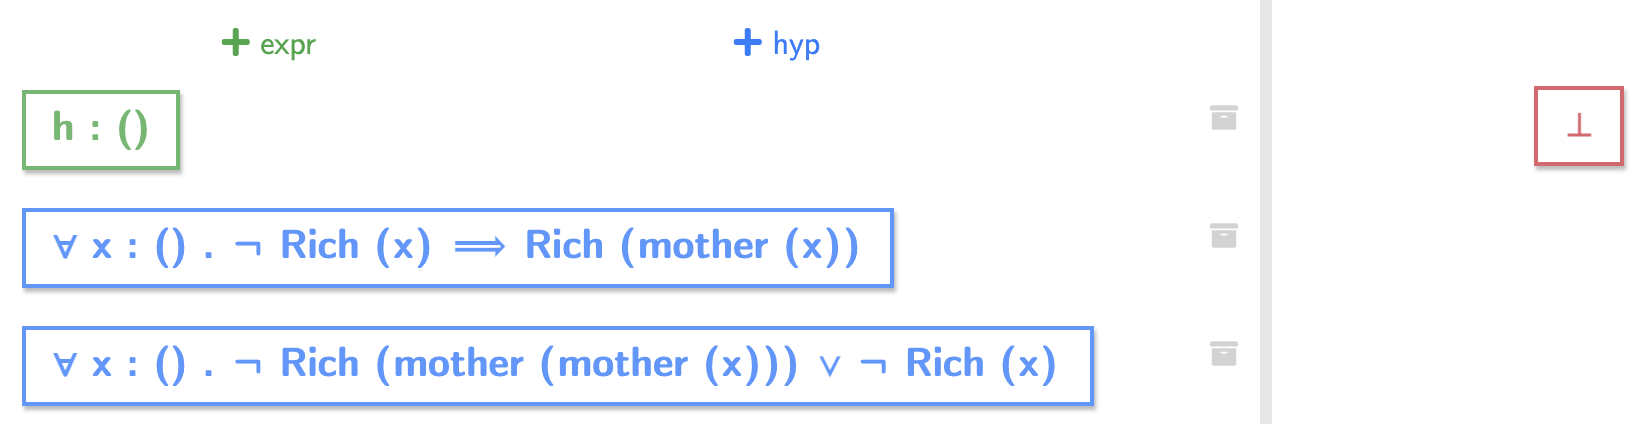
\includegraphics[width=1.3\textwidth]{edukera.png}}
  \caption{The beginning of an example due to Edukera}
  \labfig{edukera}
\end{figure*}

It is quite natural to approach this problem in a forward manner, by starting
from the hypotheses to establish new facts. And a first point illustrated by
this example is that DnD actions allow to do this in a smooth and precise
manner. A possible first step is to bring $h$ to the first hypothesis, to obtain
a new fact:

\medskip
$(3) ~\neg\rich(h)\lor \neg\rich(\mother(\mother(h))).$
\medskip

\noindent Double clicking on this new fact yields two cases:
\begin{itemize}
 \item[(4)~] $ \neg\rich(h)$,
 \item[(4')] $ \neg\rich(\mother(\mother(h)))$.
 \end{itemize}
Let us detail how one solves the
second one.

By bringing 
$\neg\rich(\mother(\mother(h)))$ on the premise of $\forall
x. \select{\neg\rich(x)} \limp \rich(\mother(x))$
one obtains

\medskip
$(6) ~\rich(\mother(\mother(\mother(h)))).$
\medskip

The next step is a good example where DnD actions are useful. By bringing this
new fact to the right-hand part of

\medskip
$(1)~\forall x. \neg\rich(x)\lor \neg\select{\rich(\mother(\mother(x)))}$
\medskip

\noindent
one immediately obtains a new fact

\medskip
$(7) ~\neg{\rich(\mother(h))}$.
\medskip

\noindent In other proof systems, this last step requires a somewhat intricate
tactic line and/or writing down at least the statement of the new fact.

One can then finish the case by combining $(7)$ and $(2)$ which yields
$$\rich(\mother(\mother(h)))$$ contradicting $(4')$. These two last steps each
correspond to a simple DnD. The other case, $\neg\rich(h)$, is quite similar.

% Such a simple example is not sufficient to provide significant metrics.
Note that once a user has understood the proof, the riddle is routinely solved
in less than a minute in Actema, which seems out of reach for about any user in
a tactic based prover. At least as important is the fact that the proof can be
performed without typing any text, especially no intermediate statement. 

To conclude this example, we propose in \reffig{edukera-coq} a complete proof of
the riddle formalized in the Coq proof assistant, which follows very closely the
structure of the graphical proof just outlined. To make the correspondence more
visible and ease the comparison, we interspersed the proof script with comments
of the form \texttt{(** [actions] *)}, where \texttt{[actions]} is a
sentence describing a sequence of actions in Actema that produces the same goal
transformation as the tactics preceding the comment. There are a few interesting
things to note:
\begin{itemize}
  \item We chose to name manually all the hypotheses introduced in the course of
  the proof. This is generally considered good practice in the Coq community,
  because it makes proof scripts easier to maintain. In our case it also has the
  advantage of expliciting which hypotheses are used exactly in the reasoning,
  something that an Actema user does with her pointing device when designating
  the blue items involved in an action. It appears clearly in
  \reffig{edukera-coq} that in a moderately long proof like this based mostly on
  forward reasoning, one needs to keep track of \emph{a lot} of names, which can
  be overwhelming for many users. This is especially true for beginners
  discovering Coq, because the syntax for assigning names, based on patterns
  like \texttt{[H | H]} that reproduce the subgoal structure, can induce a steep
  learning curve. Of course this problem is mitigated trivially in Actema, since
  names are not needed.

  \item There is no exact correspondence between the tactics of Coq and the
  actions of Actema: some tactics are simulated by multiple actions, and often a
  complex sequence of tactics can be simulated by a single action\sidenote{This
  was already noticed in \cite{PbP}, where clicking on a subformula can simulate
  a sequence of introduction rules of arbitrary length.}.
  
  For instance, line 23 does at the same time a specialization of the hypothesis
  $H_2 : \forall x. \neg \rich(\mother(\mother(x))) \lor \neg \rich(x)$ to the
  individual $h$ with the application \texttt{(H2 h)}, and a case analysis with
  the \texttt{destruct} tactic. In Actema this is performed in two steps, first
  by drag-and-dropping $h$ on $H_2$, and then by clicking on the resulting
  hypothesis\sidenote{This could also be achieved in two steps in Coq, by using
  the \texttt{specialize} tactic instead of the inlined application.}.

  In the other direction, a pattern of reasoning that occurs multiple times in
  the proof is the combination of $H_2$ with another hypothesis which
  contradicts one of the two cases, in order to deduce the truth of the other
  case. While it is captured straightforwardly in Actema with a single DnD
  between the contradictory statements, it requires in Coq a decomposition into
  many administrative steps:
  \begin{enumerate}
    \item first a case analysis with \texttt{destruct}, where the expression
    instantiating $H_2$ (e.g. $\mother(mother(h))$) needs to be written down
    explicitly, instead of being inferred automatically from unification;
    \item optionally focusing on the subgoal corresponding to the contradictory
    case if it is the right disjunct (line 56), which requires to know a
    somewhat idiosyncratic and infrequently used syntax of the tactic language;
    \item and finally expliciting the contradiction with \texttt{apply} and
    \texttt{exact}.
  \end{enumerate}

  \item More generally, the actions of Actema are more \emph{versatile} and
  \emph{context-dependent} than the tactics of Coq. For instance, click actions
  have a different effect depending on the main connective of the formula being
  clicked, but provide a unique interface for applying rules of natural
  deduction/sequent calculus. On the contrary, there is almost one tactic for
  dealing with each logical connective in Coq, e.g. \texttt{intros} for $\limp$
  and $\forall$, \texttt{split} for $\land$, \texttt{left} and \texttt{right}
  for $\lor$, \texttt{exists} for $\exists$, etc. The same remark applies to DnD
  actions, whose functionalities are provided in Coq by many different tactics:
  \texttt{apply \_}, \texttt{apply \_ in \_}, \texttt{pose proof},
  \texttt{specialize}, etc.
\end{itemize}

\begin{figure}
  % \fontsize{8}{8.5}\selectfont
  % \begin{alectryon}
  % Generator: Alectryon
  \sep
  \begin{txt}
    \PY{c}{(*~Declaration~of~constants~used~in~the~statement~of~the~riddle~*)}\nl
    \nl
  \end{txt}
  \sep
  \begin{sentence}
    \begin{input}
      \PY{k+kn}{Context}~\PY{o}{(}\PY{n+nv}{i}~\PY{o}{:}~\PY{k+kt}{Type}\PY{o}{).}\nl
    \end{input}
  \end{sentence}
  \sep
  \begin{txt}
    \nl
  \end{txt}
  \sep
  \begin{sentence}
    \begin{input}
      \PY{k+kn}{Context}~\PY{o}{(}\PY{n+nv}{Rich}~\PY{o}{:}~\PY{n}{i}~\PY{o}{\PYZhy{}\PYZgt{}}~\PY{k+kt}{Prop}\PY{o}{).}\nl
    \end{input}
  \end{sentence}
  \sep
  \begin{sentence}
    \begin{input}
      \PY{k+kn}{Context}~\PY{o}{(}\PY{n+nv}{mother}~\PY{o}{:}~\PY{n}{i}~\PY{o}{\PYZhy{}\PYZgt{}}~\PY{n}{i}\PY{o}{).}\nl
    \end{input}
  \end{sentence}
  \sep
  \begin{sentence}
    \begin{input}
      \PY{k+kn}{Context}~\PY{o}{(}\PY{n+nv}{h}~\PY{o}{:}~\PY{n}{i}\PY{o}{).}\nl
    \end{input}
  \end{sentence}
  \sep
  \begin{txt}
    \nl
    \PY{c}{(*~Statement~of~the~riddle~*)}\nl
    \nl
  \end{txt}
  \sep
  \begin{sentence}
    \begin{input}
      \PY{k+kn}{Theorem}~\PY{n+nf}{rich\PYZus{}mothers}~\PY{o}{:}\nl
      ~~\PY{o}{(}\PY{k+kr}{forall}~\PY{n+nv}{x}\PY{o}{,}~\PY{o}{\PYZti{}}\PY{n}{Rich}\PY{o}{(}\PY{n}{x}\PY{o}{)}~\PY{o}{\PYZhy{}\PYZgt{}}~\PY{n}{Rich}\PY{o}{(}\PY{n}{mother}\PY{o}{(}\PY{n}{x}\PY{o}{)))}~\PY{o}{\PYZhy{}\PYZgt{}}\nl
      ~~\PY{o}{(}\PY{k+kr}{forall}~\PY{n+nv}{x}\PY{o}{,}~~\PY{o}{\PYZti{}}\PY{n}{Rich}\PY{o}{(}\PY{n}{mother}\PY{o}{(}\PY{n}{mother}\PY{o}{(}\PY{n}{x}\PY{o}{)))}~\PY{o}{\PYZbs{}/}~\PY{o}{\PYZti{}}\PY{n}{Rich}\PY{o}{(}\PY{n}{x}\PY{o}{))}~\PY{o}{\PYZhy{}\PYZgt{}}\nl
      ~~\PY{k+kt}{False}\PY{o}{.}\nl
    \end{input}
  \end{sentence}
  \sep
  \begin{txt}
    \nl
    \PY{c}{(*~Proof~of~the~riddle~*)}
  \end{txt}
\end{alectryon}

\begin{alectryon}
  % Generator: Alectryon
  \sep
  \begin{sentence}
    \begin{input}
      \PY{k+kn}{Proof}\PY{o}{.}\nl
    \end{input}
  \end{sentence}
  \sep
  \begin{sentence}
    \begin{input}
      ~~\PY{n+nb}{intros}~\PY{n}{H1}~\PY{n}{H2}\PY{o}{.}\nl
    \end{input}
  \end{sentence}
  \sep
  \begin{txt}
    \nl
    ~~\PY{l+s+sd}{(**~2~clicks~on~the~conclusion~*)}\nl
    \nl
  \end{txt}
  \sep
  \begin{sentence}
    \begin{input}
      ~~\PY{n+nb}{destruct}~\PY{o}{(}\PY{n}{H2}~\PY{n}{h}\PY{o}{)}~\PY{k+kr}{as}~\PY{o}{[}\PY{n}{H}~\PY{o}{|}~\PY{n}{H}\PY{o}{].}\nl
    \end{input}
  \end{sentence}
  \sep
  \begin{txt}
    \nl
    ~~\PY{l+s+sd}{(**~DnD~of~[h]~onto~[H2],~then~click~on~the~resulting~hypothesis~*)}\nl
    \nl
  \end{txt}
  \sep
  \begin{sentence}
    \begin{input}
      ~~\PY{o}{*}~
    \end{input}
  \end{sentence}
  \sep
  \begin{sentence}
    \begin{input}
      \PY{n+nb}{pose~proof}~\PY{o}{(}\PY{n}{H1}~\PY{n}{\PYZus{}}~\PY{n}{H}\PY{o}{)}~\PY{k+kr}{as}~\PY{n}{H\PYZsq{}}\PY{o}{.}\nl
    \end{input}
  \end{sentence}
  \sep
  \begin{txt}
    \nl
    ~~~~\PY{c}{(*~If~one~naively~uses~[apply~\PYZus{}~in],~then~one~loses~[H]~although}\nl
    \PY{c}{~~~~~~~it~is~needed~later!~Hence~the~use~of~[pose~proof].~*)}\nl
    \nl
    ~~~~\PY{l+s+sd}{(**~DnD~of~[H1]~onto~[H]~*)}\nl
    \nl
  \end{txt}
  \sep
  \begin{sentence}
    \begin{input}
      ~~~~\PY{n+nb}{destruct}~\PY{o}{(}\PY{n}{H2}~\PY{o}{(}\PY{n}{mother}~\PY{n}{h}\PY{o}{))}~\PY{k+kr}{as}~\PY{o}{[}\PY{n}{H2\PYZsq{}}~\PY{o}{|}~\PY{n}{H2\PYZsq{}}\PY{o}{].}\nl
    \end{input}
  \end{sentence}
  \sep
  \begin{sentence}
    \begin{input}
      ~~~~\PY{n+nb}{apply}~\PY{n}{H2\PYZsq{}}\PY{o}{.}~
    \end{input}
  \end{sentence}
  \sep
  \begin{sentence}
    \begin{input}
      \PY{n+nb+bp}{exact}~\PY{n}{H\PYZsq{}}\PY{o}{.}\nl
    \end{input}
  \end{sentence}
  \sep
  \begin{txt}
    \nl
    ~~~~\PY{l+s+sd}{(**~DnD~of~[H\PYZsq{}]~onto~[H2].~Could~also~be~performed~stepwise:~~}\nl
    \PY{l+s+sd}{~~~~~~~~\PYZhy{}~Selection~of~[mother(h)]~in~[H\PYZsq{}]}\nl
    \PY{l+s+sd}{~~~~~~~~\PYZhy{}~DnD~of~[H\PYZsq{}]~onto~[H2]}\nl
    \PY{l+s+sd}{~~~~~~~~\PYZhy{}~Click~on~the~resulting~hypothesis}\nl
    \PY{l+s+sd}{~~~~~~~~\PYZhy{}~DnD~of~[H2\PYZsq{}]~onto~[H\PYZsq{}]~*)}\nl
    \nl
  \end{txt}
  \sep
  \begin{sentence}
    \begin{input}
      ~~~~\PY{n+nb}{apply}~\PY{n}{H1}~\PY{k+kr}{in}~\PY{n}{H2\PYZsq{}}\PY{o}{.}\nl
    \end{input}
  \end{sentence}
  \sep
  \begin{txt}
    \nl
    ~~~~\PY{l+s+sd}{(**~DnD~of~[H1]~onto~[H2\PYZsq{}]~*)}\nl
    \nl
  \end{txt}
  \sep
  \begin{sentence}
    \begin{input}
      ~~~~\PY{n+nb}{apply}~\PY{n}{H}\PY{o}{.}~
    \end{input}
  \end{sentence}
  \sep
  \begin{sentence}
    \begin{input}
      \PY{n+nb+bp}{exact}~\PY{n}{H2\PYZsq{}}\PY{o}{.}\nl
    \end{input}
  \end{sentence}
  \sep
  \begin{txt}
    \nl
    ~~~~\PY{l+s+sd}{(**~DnD~of~[H]~onto~[H2\PYZsq{}]~*)}\nl
    \nl
  \end{txt}
  \sep
  \begin{sentence}
    \begin{input}
      ~~\PY{o}{*}~
    \end{input}
  \end{sentence}
  \sep
  \begin{sentence}
    \begin{input}
      \PY{n+nb}{pose~proof}~\PY{o}{(}\PY{n}{H1}~\PY{n}{\PYZus{}}~\PY{n}{H}\PY{o}{)}~\PY{k+kr}{as}~\PY{n}{H\PYZsq{}}\PY{o}{.}\nl
    \end{input}
  \end{sentence}
  \sep
  \begin{txt}
    \nl
    ~~~~\PY{l+s+sd}{(**~DnD~of~[H1]~onto~[H]~*)}\nl
    \nl
  \end{txt}
  \sep
  \begin{sentence}
    \begin{input}
      ~~~~\PY{n+nb}{destruct}~\PY{o}{(}\PY{n}{H2}~\PY{o}{(}\PY{n}{mother}~\PY{n}{h}\PY{o}{))}~\PY{k+kr}{as}~\PY{o}{[}\PY{n}{H2\PYZsq{}}~\PY{o}{|}~\PY{n}{H2\PYZsq{}}\PY{o}{].}\nl
    \end{input}
  \end{sentence}
  \sep
  \begin{sentence}
    \begin{input}
      ~~~~\PY{l+m+mi}{2}\PY{o}{:}~\PY{o}{\PYZob{}}~
    \end{input}
  \end{sentence}
  \sep
  \begin{sentence}
    \begin{input}
      \PY{n+nb}{apply}~\PY{n}{H2\PYZsq{}}\PY{o}{.}~
    \end{input}
  \end{sentence}
  \sep
  \begin{sentence}
    \begin{input}
      \PY{n+nb+bp}{exact}~\PY{n}{H\PYZsq{}}\PY{o}{.}~
    \end{input}
  \end{sentence}
  \sep
  \begin{sentence}
    \begin{input}
      \PY{o}{\PYZcb{}}\nl
    \end{input}
  \end{sentence}
  \sep
  \begin{txt}
    \nl
    ~~~~\PY{l+s+sd}{(**~DnD~of~[H\PYZsq{}]~onto~[H2]~*)}\nl
    \nl
  \end{txt}
  \sep
  \begin{sentence}
    \begin{input}
      ~~~~\PY{n+nb}{pose~proof}~\PY{o}{(}\PY{n}{H1}~\PY{n}{\PYZus{}}~\PY{n}{H2\PYZsq{}}\PY{o}{)}~\PY{k+kr}{as}~\PY{n}{H2\PYZsq{}\PYZsq{}}\PY{o}{.}\nl
    \end{input}
  \end{sentence}
  \sep
  \begin{txt}
    \nl
    ~~~~\PY{l+s+sd}{(**~DnD~of~[H1]~onto~[H2\PYZsq{}]~*)}\nl
    \nl
  \end{txt}
  \sep
  \begin{sentence}
    \begin{input}
      ~~~~\PY{n+nb}{destruct}~\PY{o}{(}\PY{n}{H2}~\PY{o}{(}\PY{n}{mother}~\PY{o}{(}\PY{n}{mother}~\PY{n}{h}\PY{o}{)))}~\PY{k+kr}{as}~\PY{o}{[}\PY{n}{H2\PYZsq{}\PYZsq{}\PYZsq{}}~\PY{o}{|}~\PY{n}{H2\PYZsq{}\PYZsq{}\PYZsq{}}\PY{o}{].}\nl
    \end{input}
  \end{sentence}
  \sep
  \begin{sentence}
    \begin{input}
      ~~~~\PY{n+nb}{apply}~\PY{n}{H2\PYZsq{}\PYZsq{}\PYZsq{}}\PY{o}{.}~
    \end{input}
  \end{sentence}
  \sep
  \begin{sentence}
    \begin{input}
      \PY{n+nb+bp}{exact}~\PY{n}{H2\PYZsq{}\PYZsq{}}\PY{o}{.}\nl
    \end{input}
  \end{sentence}
  \sep
  \begin{txt}
    \nl
    ~~~~\PY{l+s+sd}{(**~DnD~of~[H2\PYZsq{}\PYZsq{}]~onto~[H2]~*)}\nl
    \nl
  \end{txt}
  \sep
  \begin{sentence}
    \begin{input}
      ~~~~\PY{n+nb}{apply}~\PY{n}{H1}~\PY{k+kr}{in}~\PY{n}{H2\PYZsq{}\PYZsq{}\PYZsq{}}\PY{o}{.}\nl
    \end{input}
  \end{sentence}
  \sep
  \begin{txt}
    \nl
    ~~~~\PY{l+s+sd}{(**~DnD~of~[H1]~onto~[H2\PYZsq{}\PYZsq{}\PYZsq{}]~*)}\nl
    \nl
  \end{txt}
  \sep
  \begin{sentence}
    \begin{input}
      ~~~~\PY{n+nb}{apply}~\PY{n}{H2\PYZsq{}}\PY{o}{.}~
    \end{input}
  \end{sentence}
  \sep
  \begin{sentence}
    \begin{input}
      \PY{n+nb+bp}{exact}~\PY{n}{H2\PYZsq{}\PYZsq{}\PYZsq{}}\PY{o}{.}\nl
    \end{input}
  \end{sentence}
  \sep
  \begin{txt}
    \nl
    ~~~~\PY{l+s+sd}{(**~DnD~of~[H2\PYZsq{}]~onto~[H2\PYZsq{}\PYZsq{}\PYZsq{}]~*)}\nl
  \end{txt}
  \sep
  \begin{sentence}
    \begin{input}
      \PY{k+kn}{Qed}\PY{o}{.}
    \end{input}
  \end{sentence}
\end{alectryon}
  \begin{minted}
  [
  frame=lines,
  framesep=2mm,
  baselinestretch=1,
  fontsize=\footnotesize,
  linenos
  ]
  {coq}

(* Declaration of constants used in the statement of the riddle *)

Context (i : Type).
Context (Rich : i -> Prop).
Context (mother : i -> i).
Context (h : i).

(* Statement of the riddle *)

Theorem rich_mothers :
  (forall x, ~Rich(x) -> Rich(mother(x))) ->
  (forall x,  ~Rich(mother(mother(x))) \/ ~Rich(x)) ->
  False.

(* Proof of the riddle *)

Proof.
  intros H1 H2.
  (** 2 clicks on the conclusion *)

  destruct (H2 h) as [H | H].
  (** DnD of [h] onto [H2], then click on the resulting hypothesis *)

  * pose proof (H1 _ H) as H'.
    (* If one naively uses [apply _ in], then one loses [H] although
       it is needed later! Hence the use of [pose proof]. *)
    (** DnD of [H1] onto [H] *)
    
    destruct (H2 (mother h)) as [H2' | H2'].
    apply H2'. exact H'.
    (** DnD of [H'] onto [H2]. Could also be performed stepwise:  
        - Selection of [mother(h)] in [H']
        - DnD of [H'] onto [H2]
        - Click on the resulting hypothesis
        - DnD of [H2'] onto [H'] *)

    apply H1 in H2'.
    (** DnD of [H1] onto [H2'] *)

    apply H. exact H2'.
    (** DnD of [H] onto [H2'] *)

  * pose proof (H1 _ H) as H'.
    (** DnD of [H1] onto [H] *)

    destruct (H2 (mother h)) as [H2' | H2'].
    2: { apply H2'. exact H'. }
    (** DnD of [H'] onto [H2] *)

    pose proof (H1 _ H2') as H2''.
    (** DnD of [H1] onto [H2'] *)

    destruct (H2 (mother (mother h))) as [H2''' | H2'''].
    apply H2'''. exact H2''.
    (** DnD of [H2''] onto [H2] *)

    apply H1 in H2'''.
    (** DnD of [H1] onto [H2'''] *)

    apply H2'. exact H2'''.
    (** DnD of [H2'] onto [H2'''] *)
Qed.

\end{minted}
  \caption{Coq proof script formalizing Edukera's riddle}
  \labfig{edukera-coq}
\end{figure}

From this detailed comparison, it appears that the interface offered by the
Proof-by-Action paradigm might be more suited to forward reasoning than the
tactic language of Coq, at least in some respects. It makes the flow of
argumentation more straightforward to express with DnD actions, and avoids the
overheads of name management and syntax memorization. This altogether shall
prove to be particularly helpful to beginners and learners of the proof
assistant.


\section{Sets and functions}\labsec{funcs}

Our second example comes from a preprint of Bartzia et al.
\cite{bartzia:hal-04087080}, where it is chosen specifically for a case study
aiming to compare the features of different proof assistants' interfaces in an
educational setting. It is ``a typical exercise about sets, relations and
functions, as commonly found in introductory courses about reasoning and
proof.'' (p. 6):

\begin{exercise}
  Given three sets $A$, $B$ and $C$ such that $C \subseteq A$ and a function $f
  : A \to B$, show that:
  \begin{enumerate}
    \item $C \subseteq f^{-1}(f(C))$.
    \item If $f$ is injective then $f^{-1}(f(C)) \subseteq C$.
  \end{enumerate}
  where $f(D)$ and $f^{-1}(E)$ denote respectively the direct and inverse image
  (or preimage) of sets $D \subseteq A$ and $E \subseteq B$ by $f$.
\end{exercise}

Compared to our previous example, this exercise has the particularity of
involving multiple \emph{definitions}, here about sets and functions between
them. There are many possible ways to handle definitions in a formal proof
system. A common one is to decompose the definition into a new function or
predicate symbol, the definition's \emph{head}, and a universally parametrized
equality or equivalence between the head and the \emph{body} of the definition.
For instance, the concept of injectivity can be encoded as a unary predicate
$\injective(\cdot)$ on functions, satisfying the following equivalence:
$$\forall A.\ \forall B.\ \forall f{:}A \to B.~\ \injective(f) ~\lequiv~ \forall x
\in A.\ \forall y \in A.\ f(x) = f(y) \limp x = y$$

Notice that $\injective(\cdot)$ is a \emph{higher-order} predicate, since it
takes any function as argument. Depending on the underlying logical framework,
this might have an impact on the exact way the definition is encoded. Here we do
not want to bother with such implementation details, and simply assume that
higher-order definitions are possible, even though Actema is currently limited
to first-order logic. In practice this does not affect the semantics of
graphical actions, and we can imagine having a first-order set theory such as
\sys{ZF} to make everything work behind the scenes\sidenote{See also
\refsec{pluginfuture} for a discussion on a higher-order extension of Actema.}.

Let us now describe how to prove the second question of the exercise in the
Proof-by-Action paradigm. The first thing we want to do is to unfold the
definition of set inclusion in the conclusion $f^{-1}(f(C)) \subseteq C$, so
that we can see how to prove logically such an inclusion. One might imagine
multiple kinds of graphical actions for doing this. In Actema we implemented a
general \emph{subterm selection} mechanism, where the user can successively
point at different subterms appearing in the goal --- either in the context or
the conclusion --- and then choose from a list of available actions taking the
selection as argument. In our case we can select the whole conclusion, and then
choose to apply the \action{Unfold} action:
$$\select{f^{-1}(f(C)) \subseteq C} \qquad \text{(\action{Unfold})}$$
The system will be able to tell that we
selected an instance of the two-place inclusion predicate $\cdot \subseteq
\cdot$, and thus will replace the head of this definition by its body,
instantiating parameters accordingly. This gives us a new conclusion
$$\forall x. x \in f^{-1}(f(C)) \limp x \in C$$
on which we can click twice to introduce a new variable $x$ in the context,
together with the hypothesis:
\begin{itemize}
  \item[(1)] $x \in f^{-1}(f(C))$
\end{itemize}

Now there is no available action on the conclusion $x \in C$, because set
membership is a \emph{primitive} predicate in set theory: it does not have any
associated definition in the sense mentioned above\sidenote{Formally, the
meaning of $\in$ in a set theory such as \sys{ZF} comes from the various axioms
involving it. One might call such a definition \emph{behavioral}, since the
meaning of the symbol emerges from the way it can be used in proofs through
axioms. In contrast, the usual notion of mathematical definition we tackle in
this chapter might be called \emph{nominal}, because it essentially amounts to
giving a name (the head) to a reoccurring pattern of statement (the body). Note
that the syntax of first-order logic is unaware of this distinction, since in
both cases the defined concepts are encoded as \emph{atomic} predicates. This is
usually not the case of logical frameworks found in proof assistants: for
instance, the duality between \emph{judgmental} (nominal) and
\emph{propositional} (behavioral) equality is at the heart of Martin-Löf's type
theory, and it is used extensively in Coq to perform automation, both in the
computation of expressions and the matching of statements modulo definitions.}.
But we can still unfold some definitions in the context, which might suggest
further possible interactions. First we can unfold the definition of preimage
used in $(1)$ by selecting the precise corresponding subterm:
$$x \in \select{f^{-1}(f(C))} \qquad \text{(\action{Unfold})}$$
which, assuming a definition based on set comprehension, gives:
\begin{itemize}
  \item[(1)] $x \in \compr{a \in A}{f(a) \in f(C)}$
\end{itemize}
At this stage, we would like to make the set comprehension in $(1)$ disappear,
by simply deducing $f(x) \in f(C)$ from it. But depending on the underlying
logical framework, the way to perform this deduction step in Proof-by-Action
will vary:

\begin{description}
  \item[In \sys{ZF} set theory]
    We would need to invoke explicitly the \emph{axiom of comprehension}, which
    states the following:
    $$\forall \phi.\ \forall D.\ \forall y.\ y \in \compr{d \in D}{\phi} ~~\lequiv~~ (y \in D \land \subst{\phi}{y}{d})$$
    Note that this is again a higher-order statement, but this time because it
    quantifies over every formula $\phi$\sidenote{Traditionnally, logicians
    preferred to speak of \emph{axiom schemas}, that is denumerable sets of
    axioms, rather than higher-order axioms, in order to stay purely in a
    first-order setting. But this does not make much sense from an
    implementation point of view, as a proof engine will only be able to
    manipulate a finite amount of axioms.}. Thus we assume that the underlying
    proof engine can handle such higher-order statements, and in particular that
    the axiom of comprehension is available in its database of lemmas.
    
    In Actema, one can freely search in this database by typing text in a search
    bar, typically in this case the keyword ``comprehension''. Then the system
    will show a list of lemmas whose names match the keywords, and the user can
    click on the lemma she is interested in, in order to add it as a blue item
    in the current context. An alternative and more precise way of retrieving a
    lemma is to search by \emph{content} of the statement instead of searching
    by name. State-of-the-art proof assistants usually provide facilities for
    this: for instance Coq has a \texttt{Search} command which can take
    \emph{patterns}, i.e. terms with holes or so-called \emph{metavariables}, in
    order to filter out results that do not match the given pattern. In Actema,
    we implemented a novel feature which replaces patterns by a selection of
    subterms in the current goal, similarly to what is given as argument to
    contextual actions like \action{Unfold}. Then the system will only look for
    lemmas which can be used in a DnD action involving precisely the current
    selection of subterms. In this case, selecting the full statement of $(1)$
    and searching:
    $$\select{x \in \compr{a \in A}{f(a) \in f(C)}} \qquad
    \text{(\action{Search})}$$
    should return the comprehension axiom among other lemmas, because this axiom
    and $(1)$ can interact through the following forward DnD:
    $$\select{x \in \compr{a \in A}{f(a) \in f(C)}} ~~\forw~~ \forall \phi.\
    \forall D.\ \forall y.\ \select{y \in \compr{d \in D}{\phi}} ~~\lequiv~~ (y
    \in D \land \subst{\phi}{y}{d})$$ by substituting $D$ with $A$, $d$ with
    $a$, $y$ with $x$ and $\phi$ with $f(a) \in f(C)$. Performing this DnD will
    finally result in a new hypothesis corresponding to the intended unfolding
    of the definition of set comprehension\sidenote{Here in the sense of a
    \emph{behavioral} definition.}:
    \begin{itemize}
      \item[(2)] $x \in A \land f(x) \in f(C)$
    \end{itemize}
  
  \item[In higher-order type theory] In type theory, every mathematical object
  or statement is ultimately encoded as a function, in the sense of the
  $\lambda$-calculus. It is Alonzo Church who first got the idea of representing
  a set by its \emph{characteristic function} in his higher-order logic, as a
  $\lambda$-term of type $\iota \to \omicron$ where $\iota$ is the type of
  individuals, and $\omicron$ the type of propositions\todo{add citation}. With
  this encoding, the only way to construct a set is by comprehension, and set
  membership corresponds to function application; that is, $\compr{x \in
  A}{\phi}$ is identified with the characteristic function $\lambda x{:}A.\
  \phi$, and $x \in t$ is the application $t\ x$\sidenote{Note that this induces
  a strict hierarchical notion of set as in Russell's type theory, where sets
  containing other sets have a higher-order type, i.e. they correspond to
  functions taking other functions as arguments.}. Then if we consider
  $\lambda$-terms modulo $\beta$-equivalence, unfolding the ``definition'' of
  set comprehension just amounts to performing one step of
  $\beta$-reduction\sidenote{One can consider this as a third kind of definition
  qualified of \emph{computational}. In Martin-Löf's type theory, it is merged
  with nominal definitions in the concept of judgmental equality. In Coq they
  are distinguished: computational and nominal definitions correspond
  respectively to $\beta$-reduction and $\delta$-reduction.}: hypothesis $(1)$
  becomes
  $$(\lambda a{:}A.\ f(C)\ f(a))\ x$$
  which $\beta$-reduces to
  $$f(C)\ f(x)$$ which we can translate back as $f(x) \in f(C)$. This encoding
  has now found its way in the libraries of many proof assistants based on type
  theory, and is the one used in the Coq solution to the exercise provided in
  annex of \cite{bartzia:hal-04087080}. To perform $\beta$-reduction in Coq,
  there is a tactic called \texttt{simpl} as in ``simplify''\sidenote{There are
  also \texttt{simp} tactics available in Isabelle and Lean, although they are
  not restricted to $\beta$-reduction and can perform rewriting of arbitrary
  equalities and equivalences present in the lemma database, as long as they are
  flagged as simplification rules.}. Coming back to Proof-by-Action, one can
  easily imagine a corresponding \action{Simplify} or \action{Compute}
  contextual action, which performs $\beta$-reduction inside of the selected
  subterm. Then the previous transormation is achieved by applying this action
  on hypothesis $(1)$:
  $$\select{x \in \compr{a \in A}{f(a) \in f(C)}} \qquad \text{(\action{Simplify})}$$
\end{description}
From a user perspective, the two styles of actions induced by the two types of
logical frameworks differ mainly in one aspect: while the definition of set
comprehension is \emph{implicit} in the type-theoretical encoding, it must be
manipulated \emph{explicitly} when using the axiom of comprehension\sidenote{In
fact one could also use the axiom of comprehension implicitly by relying on
stronger automation. For example in Isabelle/Isar, one would write explicitly
the desired goal $f(x) \in f(C)$, refer to the axiom by its name in the library,
and then let the engine find the details of how to apply it. But writing
statements manually goes against the philosophy of Proof-by-Action, which
explores to what extent proofs can be carried by pure manipulation of the proof
state. Of course there is still an escape hatch for doing this when strictly
necessary or more convenient.}. Depending on the user's background and context
of usage, one might prefer one style over the other. Typically in an educational
setting, having to manipulate explicitly the axiomatic definition might be more
instructive, but also more confusing when carrying formal proofs for the first
time.

Going back to the proof, we now have the following context of hypotheses:
\begin{itemize}
  \item[(0)] $\injective(f)$
  \item[(2)] $f(x) \in f(C)$
\end{itemize}
We can unfold the definition of direct image in $(2)$ the same way we did for
the inverse image in $(1)$: first perform the contextual action
$$f(x) \in \select{f(C)} \qquad \text{(\action{Unfold})}$$
which gives us
\begin{itemize}
  \item[(2)] $f(x) \in \compr{b \in B}{\exists a \in A.\ a \in C \land b = f(a)}$
\end{itemize}
Then we can simplify the set comprehension with
$$\select{f(x) \in \compr{b \in B}{\exists a \in A.\ a \in C \land b = f(a)}} \qquad \text{(\action{Simplify})}$$
which gives us
\begin{itemize}
  \item[(3)] $\exists a \in A.\ a \in C \land f(x) = f(a)$
\end{itemize}
Now since $f$ is injective, we should be able to deduce that $x = a$. First we
unfold the definition of injectivity in $(0)$:
$$\select{\injective(f)} \qquad \text{(\action{Unfold})}$$
which gives us
\begin{itemize}
  \item[(0)] $\forall y \in A.\ \forall z \in A.\ f(y) = f(z) \limp y = z$
\end{itemize}
Then we can use injectivity with the following forward DnD between $(0)$ and
$(3)$:
$$\forall y \in A.\ \forall z \in A.\ \select{f(y) = f(z)} \limp y = z ~~\forw~~ \exists a \in A.\ a \in C \land \select{f(x) = f(a)}$$
which gives us immediately that $x = a$ in
\begin{itemize}
  \item[(4)] $\exists a \in A.\ a \in C \land x = a$
\end{itemize}
The last steps consist in clicking twice on $(4)$ to introduce $a$ in the
context together with
\begin{itemize}
  \item[(5)] $a \in C \land x = a$
\end{itemize}
doing a backward DnD with $(5)$ to rewrite $x$ in the conclusion into $a$:
$$a \in C \land \select{x} = a ~~\back~~ \select{x} \in C$$
and finally a backward DnD with $(5)$ to conclude the proof:
$$\select{a \in C} \land x = a ~~\back~~ \select{a \in C}$$

For the sake of completeness, we included in \reffig{funset-defs},
\reffig{funset-q1} and \reffig{funset-q2} a Coq formalization of the
definitions, solution to the first question, and solution to the second question
of the exercise, respectively. We simply took the data provided in
\cite{bartzia:hal-04087080}, and added corresponding Actema actions below tactic
invokations, as in the previous section. It is quite close to the graphical proof
just outlined for the second question, hence we do not add further commentary.

\begin{figure}
  \begin{minted}
  [
  frame=lines,
  framesep=2mm,
  baselinestretch=1,
  fontsize=\footnotesize,
  linenos
  ]
  {coq}

Definition Ens {A : Type} := A -> Prop.

Definition subset {A : Type} (C D : Ens) :=
  forall (x : A), C x -> D x.

Infix "⊆" := subset (at level 30).

Definition image {A B : Type} (f : A -> B) (C : Ens) : Ens :=
  fun y => exists x, C x /\ y = f x.

Definition preimage {A B : Type} (f : A -> B) (C : Ens) : Ens :=
  fun x => C (f x).

Definition injective {A B : Type} (f : A -> B) :=
  forall x x', f x = f x' -> x = x'.

Context (A B : Type).

\end{minted}
  \caption{Preliminary definitions in Coq of an exercise on abstract functions}
  \labfig{funset-defs}
\end{figure}

\begin{figure}
  \begin{minted}
  [
  frame=lines,
  framesep=2mm,
  baselinestretch=1,
  fontsize=\footnotesize,
  linenos
  ]
  {coq}

Theorem subset_preimage_image (f : A -> B) :
  forall C, C ⊆ preimage f (image f C).
Proof.
  intros C.
  (** Click on conclusion *)

  unfold subset.
  (** Select conclusion, then apply Unfold from contextual action menu *)
  intros a H.
  (** Two clicks on conclusion *)

  unfold preimage.
  (** Select conclusion, then apply Unfold from contextual action menu *)
  unfold image.
  (** Select conclusion, then apply Unfold from contextual action menu *)
  exists a.
  split.
  apply H.
  (** DnD of [H] on [C(x)] in conclusion *)
  reflexivity.
  (** Click on conclusion *)
Qed.

\end{minted}
  \caption{Solution in Coq to the first question of an exercise on abstract functions}
  \labfig{funset-q1}
\end{figure}

\begin{figure}
  \begin{minted}
  [
  frame=lines,
  framesep=2mm,
  baselinestretch=1,
  fontsize=\footnotesize,
  linenos
  ]
  {coq}

Theorem preimage_image_subset (f : A -> B) :
  injective f -> forall C, preimage f (image f C) ⊆ C.
Proof.
  intros Hinj C.
  (** 2 clicks on conclusion *)

  unfold subset.
  (** Select conclusion, then apply Unfold from contextual action menu *)
  intros x H.
  (** 2 clicks on conclusion *)

  unfold preimage in H.
  (** Select [H], then apply Unfold from contextual action menu *)
  unfold image in H.
  (** Select [H], then apply Unfold from contextual action menu *)
  destruct H as [x' [H1 H2]].
  apply Hinj in H2.
  (** Here we need to unfold [injective] so that Actema detects a possible DnD action:
      1. Select [Hinj], then apply Unfold from contextual action menu
      2. Click on [H]
      3. DnD of [H] on [f x = f x'] in [Hinj] *)
  rewrite <- H2 in H1.
  (** DnD of last hypothesis on the leftmost [x] in [H] *)
  apply H1.
  (** DnD of last hypothesis on conclusion *)
Qed.

\end{minted}
  \caption{Solution in Coq to the second question of an exercise on abstract functions}
  \labfig{funset-q2}
\end{figure}


\section{Peano arithmetic}\labsec{arith}

In our last example, we will analyse a common proof often taught in logic
courses: the commutativity of addition in Peano arithmetic. The novelty compared
to previous examples is that it involves reasoning by \emph{induction}, which
usually has special support in mainstream proof assistants. In the
Proof-by-Action paradigm, it seems natural to map it to a special contextual
action \action{Induction}, whose availability and effect will depend on the
selected subterm. One could also imagine manipulating explicitly induction
schemes as blue items, in the same way we did for the axiom of comprehension in
the previous section. In this section we focus on describing features of the
more convenient contextual action.

First and foremost, it only makes sense to apply induction to a variable which
is quantified \emph{universally}, either because it appears in the context, or
because it is bound by a $\forall$ in the conclusion. In the first case, one can
access the contextual action in Actema by selecting the green item corresponding
to the variable; in the latter case, by selecting the subterm of the conclusion
whose head connective is the binding $\forall$\sidenote{In the standalone
version of Actema, induction is performed by clicking directly on green items,
rather than through a contextual action.}. This could also work by selecting any
occurrence of the variable regardless of its binding point, since the system can
always infer it. The only condition is that if the variable is bound by a
$\forall$, it must occur in a \emph{strictly positive} location, i.e. in the
conclusion and not on the left of an implication $\limp$. Obviously the variable
should also be of an \emph{inductive} type, i.e. one which is mapped to an
induction scheme in the system\sidenote{The standalone version of Actema only
supports induction on natural numbers, but in a proof assistant like Coq or Lean
one can easily check if a given type is inductive.}. Then the \action{Induction}
action will simply apply the associated induction scheme. In our commutativity
example, we can thus start the proof like so:
$$\select{\forall n \in \nats.\ \forall m \in \nats.\ n + m = m + n} \qquad
\text{(\action{Induction})}$$
which performs an induction on $n$, generating the two following subgoals:
$$\forall m \in \nats.\ 0 + m = m + 0 \qquad \text{and} \qquad \forall m \in \nats.\ \suc{n} + m = m + \suc{n}$$
where $S(n)$ denotes the successor of $n$, and the second subgoal has a new
variable $n \in \nats$ in its context, together with the induction hypothesis
\begin{itemize}
  \item[(1)] $\forall x \in \nats.\ n + x = x + n$
\end{itemize}
The proofs of the two subgoals can be done by induction on $m$. We focus on the
second one, which is a bit more involved. As mentioned above, an alternative way
of performing induction is to first introduce $m$ in the context by clicking on
the conclusion, and then selecting it to access the contextual action:
$$\select{m \in \nats} \qquad \text{(\action{Induction})}$$
which generates again two new subgoals:
$$S(n) + 0 = 0 + S(n) \qquad \text{and} \qquad S(n) + S(m) = S(m) + S(n)$$ where
the second subgoal has a new variable $m \in \nats$ in its context, together
with the induction hypothesis
\begin{itemize}
  \item[(2)] $S(n) + m = m + S(n)$
\end{itemize}
Let us now focus on the first subgoal. Once again, as with set comprehension in
the previous section, the addition operation may have a more \emph{axiomatic} or
more \emph{computational} definition, depending on the underlying logical
framework and library used. For instance in Coq's standard library, it is
implemented as a \emph{program} built by recursion on the left-hand argument.
Thus in this setting, if one performs computation in the whole conclusion like
so:
$$\select{S(n) + 0 = 0 + S(n)} \qquad \text{\action{Simplify}}$$
this will give a new conclusion
$$S(n + 0) = S(n)$$
where the addition program was able to automatically evaluate $S(n) + 0$ to $S(n
+ 0)$ on the left-hand side of the equality, and $0 + S(n)$ to $S(n)$ on the
right-hand side. If the proof engine does not offer such a level of automation,
one can always fallback to using Peano axioms manually, provided they are
available in the lemma database. As we have already seen, the most convenient
way to do this in the Proof-by-Action paradigm is to perform a \action{Search}
action. For example to evaluate $S(n) + 0$, one might first select it in the
conclusion and then make a search query:
$$\select{S(n) + 0} = 0 + S(n) \qquad \text{(\action{Search})}$$
Among the results which are Peano axioms, one will only find the following
ones:
\begin{itemize}
  \item[(a)] $\forall x.\ 0 \not= S(x)$
  \item[(b)] $\forall x.\ \forall y.\ S(x) = S(y) \limp x = y$
  \item[(c)] $\forall x.\ \forall y.\ S(x) + y = S(x + y)$
\end{itemize}
because the other axioms do not contain any subterm that could form a
\emph{valid} backward linkage with the selection\sidenote{See \refsec{validity}
for the notion of validity of a linkage.}. Of course we are interested in axiom
$(c)$, which we can use through the following backward DnD:
$$\forall x.\ \forall y.\ \select{S(x) + y} = S(x + y) ~~\back~~ \select{S(n) + 0} = 0 + S(n)$$
in order to rewrite $S(n) + 0$ into $S(n + 0)$ in the conclusion.

Now notice that the addition program earlier was not able to evaluate $n + 0$ to
$n$. This is because $0$ occurs on the right-hand side of $+$, and the program
is not aware of the commutativity of addition, which is precisely what we are
trying to prove. Fortunately, we can apply our induction hypothesis on $n$
$(1)$, with the following backward DnD:
$$\forall x \in \nats.\ \select{n + x} = x + n ~~\back~~ S(\select{n + 0}) = S(n)$$
which rewrites $n + 0$ into $0 + n$ in the conclusion:
$$S(0 + n) = S(n)$$
Now we can continue the computation:
$$S(\select{0 + n}) = S(n) \qquad \text{(\action{Simplify})}$$
and conclude the base case of the induction on $m$ by reflexivity, by clicking
on the conclusion $S(n) = S(n)$.

The inductive case of the induction on $m$ works similarly, but obviously we
will also need to use the induction hypothesis on $m$ $(2)$. First we compute
everywhere we can in the conclusion:
$$\select{S(n) + S(m) = S(m) + S(n)} \qquad \text{\action{Simplify}}$$
% which gives the new conclusion
% $$\select{S(n + S(m)) = S(m + S(n))} \qquad \text{\action{Simplify}}$$
Then we can apply the induction hypothesis on $n$ $(1)$:
$$\forall x.\ \select{n + x} = x + n ~~\back~~ S(\select{n + S(m)}) = S(m + S(n))$$
and also the induction hypothesis on $m$ $(2)$:
$$S(n) + m = \select{m + S(n)} ~~\back~~ S(S(m) + n) = S(\select{m + S(n)})$$
Again we compute everywhere:
$$\select{S(S(m) + n) = S(S(n) + m)} \qquad \text{(\action{Simplify})}$$
apply the induction hypothesis on $n$ $(1)$ once again:
$$\forall x.\ n + x = \select{x + n} ~~\back~~ S(S(\select{m + n})) = S(S(n + m))$$
and conclude by reflexivity on $S(S(n + m)) = S(S(n + m))$.

\begin{figure}
  \begin{minted}
  [
  frame=lines,
  framesep=2mm,
  baselinestretch=1,
  fontsize=\footnotesize,
  linenos
  ]
  {coq}

Theorem add_comm :
  forall (n m : nat), n + m = m + n.
Proof.
  induction n as [|n IHn].
  (** Select conclusion, then apply Induction from contextual action menu *)

  * induction m as [|m IHm].
    (** Select conclusion, then apply Induction from contextual action menu *)
    - reflexivity.
      (** Click on conclusion *)
    - simpl.
      (** Select conclusion, then apply Simplify from contextual action menu *)
      rewrite <- IHm.
      (** DnD of [IHm] on conclusion *)
      reflexivity.
      (** Click on conclusion *)

  * induction m as [|m IHm].
    (** Select conclusion, then apply Induction from contextual action menu *)
    - simpl.
      (** Select conclusion, then apply Simplify from contextual action menu *)
      rewrite IHn.
      (** DnD of [IHn] on conclusion *)
      reflexivity.
      (** Click on conclusion *)
    - simpl.
      (** Select conclusion, then apply Simplify from contextual action menu *)
      rewrite IHn.
      (** DnD of [IHn] on conclusion *)
      rewrite <- IHm.
      (** DnD of [IHm] on conclusion *)
      simpl.
      (** Select conclusion, then apply Simplify from contextual action menu *)
      rewrite IHn.
      (** DnD of [IHn] on conclusion *)
      reflexivity.
      (** Click on conclusion *)
Qed.

\end{minted}
  \caption{Proof of commutativity of addition on natural numbers in Coq}
  \labfig{coq-peano}
\end{figure}

As in previous sections, the interested reader can find a complete Coq
formalization in \reffig{coq-peano}, which follows the same structure as the
graphical proof just outlined. In this case the correspondence between Coq
tactics and graphical actions is almost exact. This suggests that designing a
compiler from proofs-by-action to Coq proof scripts might be a reasonable
endeavor. It will indeed be one of the subjects of \refch{plugin}.
% !TEX root =index.tex
\setchapterpreamble[u]{\margintoc}
\chapter{Parallel Conclusions and Classical Logic}
\labch{sfl-classical}

In virtually every \kl{proof assistant}, the \kl{goals} the user is faced with are
\kl{sequents} of the form $\Gamma \seq C$, with a \emph{single} conclusion $C$ to be
proved under many hypotheses in $\Gamma$. Historically, this form of \kl{sequent} was
introduced by Gentzen to formalize the rules of \kl{intuitionistic} logic in his
\kl{sequent calculus} \kl{LJ}. But his main interest was in \kl{classical} logic, as
\kl{intuitionistic} logic was still in its infancy and almost all of mathematics had
been developed in a \kl{classical} setting. Interestingly, he found that the right
syntax to develop a rich metatheory of his \kl{classical} \kl{sequent calculus} \kl{LK}
consisted in \emph{multi-conclusion} \kl{sequents} of the form $\Gamma \seq \Delta$,
where $\Delta$ is a list of conclusions that should be read
\emph{disjunctively}. That is, a \kl{sequent}
$$A_1, \ldots, A_n \seq C_1, \ldots, C_m$$
has the same meaning as the formula
$$\bigwedge_{i=1}^{n}{A_i} \limp \bigvee_{j=1}^{m}{C_j}$$

\begin{marginfigure}
  \begin{mathpar}
    \R[\lor R]
      {\Gamma \seq A, B, \Delta}
      {\Gamma \seq A \lor B, \Delta}
  \end{mathpar}
  \caption{Multiplicative \kl{right introduction rule} for disjunction}
  \labfig{multintro}
\end{marginfigure}

\begin{marginfigure}
  \begin{mathpar}
    \R[\lor R]
      {\R[{\limp}R]
        {\R[ax]
          {}
          {A \seq \select{A}, \bot}}
        {\seq A, \select{\neg A}}}
      {\seq \select{A \lor \neg A}}
  \end{mathpar}
  \caption{Proof of the excluded middle in \kl{LK}}
  \labfig{lk-tnd}
\end{marginfigure}

One way to get a multi-conclusion \kl{sequent} in \kl{LK} is to apply the
``multiplicative''\sidenote{Terminology borrowed from linear logic, where
{\rnm{\lor R}} is exactly the \kl{right introduction rule} for multiplicative
disjunction $\parr$.} \kl{introduction rule} {\kl{\lor R}} (\reffig{multintro}).
For instance, \reffig{lk-tnd} shows a proof of the \kl{law of excluded middle},
where for each rule we squared the principal formula.
% Following the mapping of click actions to \kl{sequent calculus} rules
% (\reftab{click-rules}),
One could imagine performing the same proof in \kl{Actema} by successively clicking
on these principal formulas, following a bottom-up reading of the \kl{sequent
calculus} derivation seen as the trace of a proof search process. First we decide
to prove $A \lor \neg A$: this amounts to proving alternatively $A$ or $\neg
A$, which now appear as two separate red items in the same tab. Then we try to
prove $\neg A$, with the usual method of supposing $A$ to find a contradiction.
However instead of a contradiction, we decide to backtrack and prove the
alternative conclusion $A$, which is now trivial by assumption. We come back to
these multi-conclusion click actions in \refsec{classical-click}.

It is clear in the proof that the negative occurrence of $A$ in $\neg A$ is the
one that becomes the assumption $A$ that justifies the conclusion $A$ in the
last step. It would be natural to specify this causal relationship by linking
directly the two occurrences of $A$, as we do with \kl{DnD} actions in \kl{Actema}.
However for this to be possible, we need to introduce a new \kl{interaction operator} ---
let us note it $\para$ --- that works between two conclusions, where $A \para B$
is obviously interpreted as $A \lor B$. Then after clicking on $A \lor \neg A$
we can just finish the proof by connecting $A$ and $\neg A$:
$$\select{A} \para \neg \select{A} ~~\steps{}~~ \top$$

This would avoid the additional step of clicking on $\neg A$ to turn it into an
hypothesis, and suggests the possibility of a more general behavior
associated to this $\para$ operator for arbitrary logical connectives. This is
what we explore in \refsec{classical-dnd}.

\section{Backtracking}\labsec{sfl-backtracking}

% \begin{marginfigure}
%   \begin{mathpar}
%     \R[raa]
%       {\Gamma, \neg A \seq \bot}
%       {\Gamma \seq A}
%   \end{mathpar}
%   \caption{Rule of \textit{reductio ad absurdum}}
%   \labfig{raa}
% \end{marginfigure}

Interestingly, the \kl{classical} aspect of the proof of $A \lor \neg A$ in
\reffig{lk-tnd} comes exclusively from the \emph{backtracking} operation during
the last step, a phenomemon which is well known in the literature on
constructive/computational properties of \kl{classical} logic\todo{add references}.
Then one can see the \kl{introduction rules} {\rnm{\lor R_1}} and {\rnm{\lor R_2}},
and the restriction of \kl{intuitionistic} \kl{sequents} to one conclusion, as ways to
prevent such backtracking by forcing the choice of disjunct to prove at an early
stage.
% \sidenote{Although the ability to backtrack can be reintroduced in other
% ways, for example with the rule of \textit{reductio ad absurdum} (\reffig{raa})
% (TODO: add reference).}.

In fact backtracking can still be performed in \kl{intuitionistic} logic, but at the
meta-level of the proof search process instead of the object-level of \kl{inference
rules}. In an \kl{interactive theorem prover}, this corresponds to the ability for the
user to \emph{undo} an inference and go back to a previous \kl{proof state}. However
keeping track of the times we undo/redo inferences is very hard to do as humans,
and the user interfaces of current \kl{proof assistants} do not provide any mechanism
for it either. This has already been noted by Ayers\sidenote{Section 3.1.3 of
his thesis \cite{ayers_thesis}.}, and is a good motivation for trying to design
\kl{proof systems} where the need for meta-level backtracking is reduced, or even
removed. One way to do this is to maximize the proportion of \kl{inference rules}
that are \emph{\kl{invertible}}, meaning that their premisses always follow from
their conclusion. Indeed when looking at rules as \kl{tactics} (see \refsec{itps}),
it means that they will always reduce a provable \kl{goal} to provable \kl{subgoals}, and
thus can never induce a backtracking point\sidenote{Except of course if the user
deems the \kl{subgoal} too complex to prove in its current form, and explicitly wants
to backtrack to shape it differently.}. The {\rnm{\lor R}} rule is an example of
\kl{invertible} rule, and in \kl{LK} it can replace the other, non-\kl{invertible} rules
{\rnm{\lor R_1}} and {\rnm{\lor R_2}}.

But {\rnm{\lor R}} requires multi-conclusion sequents, and Gentzen restricted
their use to \kl{classical} logic. It turns out that logicians after Gentzen have
proposed various multi-conclusion \kl{sequent calculi} that work for \kl{intuitionistic}
logic, the most famous being \kl{GHCP} from Dragalin
\sidecite{dragalin_mathematical_1990}, which uses {\rnm{\lor R}}. In the rest of
this chapter, we will consider to what extent one can benefit from having
multiple conclusions in an \kl{intuitionistic} setting.

\section{Implementation in theorem provers}

Despite the aforementioned benefits of multi-conclusion sequents, we do not know
of any \kl{proof assistant}, whether \kl{classical} or \kl{intuitionistic}, that exposes them
in its user interface. One reason is that most proof/\kl{tactic} languages are based
on the rules of \kl{natural deduction}, which use single-conclusion sequents. Another
reason is that having one conclusion removes the need to designate it with an
explicit name or number, as is the case with hypotheses\sidenote{The current
trend is to have user-chosen or automatically generated strings for names as in
Coq and \kl{Lean}, but some provers like \kl{HOL Light} ask for the position in the list
as an integer to designate a particular hypothesis.}. And the explicit handling
of names in \kl{tactic} invokations is known to be tedious and time-consuming, to the
point that some \kl{tactic} languages like \ssreflect have been designed around this
problem \sidecite{SSR}. Thus having multiple conclusions would only double the
effort for no compelling reason.

However in our graphical paradigm based on \kl{direct manipulation}, hypotheses and
conclusions are designated by the act of \emph{pointing} at them with a mouse,
finger or any other pointing device\sidenote{With the recent advances in natural
language processing and voice recognition, one could also imagine a system based
on the selection of subterms by spelling their content. Then click and \kl{DnD}
actions could be triggered by voice commands once the subterms they apply to
have been selected. This could be an important alternative for users with
impaired vision and/or motricity.}. This opens up the possibility of exposing
multiple conclusions in the interface with associated graphical proof actions,
as outlined in the introductory example on the excluded middle. While we did not
implement such an extension, we explore in the following sections its design,
and the theoretical foundations behind it.

\section{Click actions}\labsec{classical-click}

In \reftab{click-rules}, we showed how click actions in \kl{Actema} are in direct
correspondance with the rules of the single-conclusion \kl{sequent calculus} \kl{LJ}
for \kl{intuitionistic} logic. Following the literature mentioned earlier, we just
need to replace two actions/\kl{introduction rules} to get a multi-conclusion system
capturing either \kl{intuitionistic} or \kl{classical} \kl{first-order logic}:

\begin{marginfigure}
  \begin{mathpar}
    \R[{\limp}R*c]
      {\Gamma, A \seq B, \Delta}
      {\Gamma \seq A \limp B, \Delta}
    \and
    \R[{\limp}R*i]
      {\Gamma, A \seq B}
      {\Gamma \seq A \limp B, \Delta}
  \end{mathpar}
  \caption{Multi-conclusion \kl{right introduction rules} for implication}
  \labfig{multi-imp-intro}
\end{marginfigure}

\begin{itemize}
  \item clicking on a red disjunction $A \lor B$ breaks it into two conclusions
  $A$ and $B$. This is the dual behavior to click actions on blue conjunctions,
  and corresponds to the {\rsf{\lor R}} rule of \reffig{multintro}, which is
  common to both the \kl{intuitionistic} and \kl{classical} variants;
  \item as before, clicking on a red implication $A \limp B$ breaks it into an
  hypothesis $A$ and a conclusion $B$. Without further changes, this corresponds
  to the \kl{right introduction rule} from the \kl{classical} \kl{sequent
  calculus} \kl{LK} of Gentzen (named {\rsf{{\limp}R*c}} in
  \reffig{multi-imp-intro}), and our set of actions becomes a \kl{proof system}
  for \kl{classical} logic. To go back to \kl{intuitionistic} logic, one needs
  the additional behavior that all the other conclusions of the \kl{goal} are
  removed. This corresponds to the \kl{right introduction rule} from the
  \kl{GHCP} calculus of Dragalin (named {\rsf{{\limp}R*i}} in
  \reffig{multi-imp-intro}).
\end{itemize}

\begin{remark}
  In the special case of \kl{intuitionistic} \kl{sequents} with one conclusion, the two
  variants {\rsf{{\limp}R*c}} and {\rsf{{\limp}R*i}} collapse into the usual
  {\rsf{{\limp}R}} rule.
\end{remark}
Note that we only modified the behavior of the disjunction $\lor$ and
implication $\limp$ connectives; and for the latter, only in the case when there
are at least two parallel conclusions, and thus implicitly a disjunction. Then
it is interesting to notice that the \kl{classical} behavior of the other connectives
($\bot, \land, \forall, \exists$) essentially arises from their interaction with
(positive) disjunctive statements.

If we stick to \kl{intuitionistic} logic, the benefits of having multiple conclusions
are unclear. Indeed while the {\rsf{\lor R}} rule is \kl{invertible}, the
{\rsf{{\limp}R*i}} rule is not, and thus at some point the choice of which
conclusion to prove must be made by the user irreversibly, even if the choice is
delayed\sidenote{In \refsec{colors}, we will see how to overcome this limitation
by using a \emph{\kl{nested sequent}} system.}. On the other hand the
{\rsf{{\limp}R*c}} rule \emph{is} \kl{invertible}: this is known to allow the
formulation of \kl{sequent calculi} for \kl{classical} logic where \emph{all} rules are
\kl{invertible}, like the \kl{G3c} calculus of \sidecite{negri_structural_2001}. In
the propositional case, this gives a constructive decision procedure for the
question of provability: given a \kl{sequent} $\Gamma \seq \Delta$, one just has to
choose any formula in $\Gamma$ or $\Delta$ and apply the \kl{introduction rule}
associated to its main connective, or the axiom rule whenever possible. In
Actema, this would correspond to having the user click randomly on blue and red
items until all \kl{goals} are solved. The procedure ends because all \kl{introduction
rules} destroy the main connective, and none of them duplicate formulas: thus the
total size of the \kl{sequent} decreases strictly after each rule application.

\begin{marginfigure}
  \begin{mathpar}
    \R[\forall L*]
      {\Gamma, \forall x. A, \subst{A}{t}{x} \seq \Delta}
      {\Gamma, \forall x. A \seq \Delta}
    \and
    \R[\exists R*]
      {\Gamma \seq \subst{A}{t}{x}, \exists x. A, \Delta}
      {\Gamma \seq \exists x. A, \Delta}
  \end{mathpar}
  \caption{Multi-conclusion instantiation rules for quantifiers}
  \labfig{multi-inst}
\end{marginfigure}

When dealing with quantifiers, the situation is not so simple: if one wants
\kl{invertible} \kl{introduction rules}, it is necessary to duplicate the quantified
formula being instantiated, which can be seen as the root cause of
undecidability in \kl{predicate logic} as noted by
Girard\cite[Section~3.3.2]{girard:hal-01322183}. This is already what happens in
Actema for the universal quantifier: dropping a term $t$ on a blue item $\forall
x. A$ will produce a new hypothesis $\subst{A}{t}{x}$, while keeping the
original $\forall x. A$ item. This corresponds to the \kl{invertible}
\kl{left introduction rule} of \kl{G3c} ({\rsf{\forall L*}} in \reffig{multi-inst}).
But in the single-conclusion framework, dropping a term $t$ on a red item
$\exists x. A$ necessarily replaces it by the instantiated conclusion
$\subst{A}{t}{x}$. Allowing multiple conclusions circumvents this problem and
restores the symmetry between $\forall$ and $\exists$, since we can create a new
conclusion for $\subst{A}{t}{x}$ while preserving the old one. This corresponds
to the \kl{invertible} \kl{right introduction rule} of \kl{G3c} ({\rsf{\exists R*}} in
\reffig{multi-inst}).

\section{DnD actions}\labsec{classical-dnd}

Once we allow for more than one conclusion, it is natural to wonder whether it
makes sense to also allow for \kl{DnD} actions between two conclusions. But we
already capture \emph{\kl{backward}} reasoning with the $A \back B$ operator between
a hypothesis $A$ and a conclusion $B$, and \emph{\kl{forward}} reasoning with the $A
\forw B$ operator between two hypotheses. There does not seem to be room for a
third mode of reasoning, at least in the traditional way of building proofs we
are used to, either on paper or with \kl{proof assistants}. However from a purely
formal point of view, there is nothing preventing us from trying to design
\kl{rewriting rules} for a new \kl{interaction operator}, by following the same recipe we used
for $\back$ and $\forw$. Furthermore, we already saw earlier in the excluded
middle example that such an operator did seem useful.

When looking for a proof of a \kl{sequent} with multiple conclusions, unless we
commit to proving one conclusion and give up on the others by applying the
{\rsf{{\limp}R*i}} rule, we can switch freely our focus between the different
conclusions. Thus in a way, we are looking for proofs of all the conclusions
\emph{in parallel}, and we stop as soon as we find one\sidenote{This is also
related to the $\parr$ connective of linear logic which uses the {\rsf{\lor
R}} rule of \reffig{multintro}, and whose spelling ``par'' is historically
motivated by an understanding of the multiplicative fragment of \kl{LL} as a
logic of parallel computation \cite{girard-linear-1987}.}. Hence we chose to
call this third kind of interaction between two conclusions \emph{parallel}
reasoning. This justifies the choice of notation for the parallel \kl{interaction
operator} $\para$, which is suggestive of the parallel composition $\mid$ from
process calculi.

The rules governing $\para$ are presented in \reffig{parallel}. A parallel
\kl{linkage} can be created either by drag-and-dropping two conclusions together, or
through an instance of the new \kl(dnd){backward} rule {\rsf{L{\limp}_1}}. It is
important to note that this rule is only sound \emph{\kl{classically}}; indeed we can
now come back to the example of \refsubsec{polarity} and give the following
derivation of Peirce's law with it:

$$
\begin{array}{llll}
  (\select{A} \limp B) \limp A \back \select{A}
  &\step{}& (\select{A} \limp B \para \select{A}) \land (A \limp A) &\mathsf{L{\limp}_1} \\
  &\step{}& ((\select{A} \back \select{A}) \lor B) \land (A \limp A) &\mathsf{P{\limp}_1} \\
  &\step{}& (\top \lor B) \land (A \limp A) &\mathsf{id} \\
  &\step{}& \top \land (A \limp A) &\mathsf{absl} \\
  &\step{}& A \limp A &\mathsf{neul}
\end{array}
$$

\begin{marginfigure}
  \fontsize{9}{9.5}\selectfont
    \renewcommand{\arraystretch}{1.25}
  \begin{mathpar}
    \begin{array}{r@{\,}c@{\,}lr}
      \multicolumn{4}{c}{\textsc{\kl(dnd){Backward}}} \\[2em]
      {B \limp C \back A}   &\step{}&   {(B \para A) \land (C \limp A)} &\mathsf{L{\limp}_1} \\[2em]
    \end{array}
    \\
    \begin{array}{r@{\,}c@{\,}lr}
      \multicolumn{4}{c}{\textsc{Parallel}} \\[2em]
      % \R[\mathsf{lnn}]
      %   {\ifill{\eta}{\efill{A}{A} \ast \efill{B}{B}}}
      %   {\ifill{\eta}{\ifill{A}{A} \land \ifill{B}{B}}}
      % \\
      {A \para (B \land C)}   &\step{}&   {(A \para B) \land C}   &\mathsf{P\land_1}\\
      {A \para (C \land B)}   &\step{}&   {C \land (A \para B)}   &\mathsf{P\land_2}\\[1em]

      {A \para (B \lor C)}   &\step{}&   {A \para B}   &\mathsf{P\lor_1}\\
      {A \para (C \lor B)}   &\step{}&   {A \para B}   &\mathsf{P\lor_2}\\[1em]

      {A \para (B \limp C)}   &\step{}&    {(B \back A) \lor C}   &\mathsf{P\!\!\limp_1}\rever\\
      {A \para (C \limp B)}   &\step{}&    {C \limp (A \para B)}   &\mathsf{P\!\!\limp_2}\rever\\[1em]

      % {A \para \neg B}   &\step{}&   {B \back A}   &\mathsf{P\neg}\rever\\[1em]

      {A \para (\forall x. B)}   &\step{}&{\forall x. (A \para B)}   &\mathsf{P\forall s}\rever\\[1em]

      {A \para (\exists x. B)}   &\step{}&   {A \para \subst{B}{x}{t}}   &\mathsf{P\exists i}\\
      {A \para (\exists x. B)}   &\step{}&   {\exists x. (A \para B)}   &\mathsf{P\exists s}\rever\\[1em]
            
      {B \para A}   &\step{}&   {A \para B}   &\mathsf{Pcomm}\\
    \end{array}
  \end{mathpar}
  ~\\[1em]
  In the rules $\{\mathsf{P \forall s}, \mathsf{P \exists s}\}$, $x$ is not free
  in $A$.
  ~\\[1em]
  \caption{Parallel linking rules}
  \labfig{parallel}
\end{marginfigure}

\begin{marginfigure}
  \begin{center}
  % https://tikzcd.yichuanshen.de/#N4Igdg9gJgpgziAXAbVABwnAlgFyxMJZABgBpiBdUkANwEMAbAVxiRADEQBfU9TXfIRQAmclVqMWbAArdeIDNjwEiARjHV6zVohAAhbuJhQA5vCKgAZgCcIAWyRkQOCElEgARjDBQkAZicGOi8GaX5lIRAGGEscEE1JHQ5AYKJVOStbB0R3FyR1T29fRACE7TYAGVT0kBt7POpc7OovH38nLSldaSqeDLqm51dEJxaikoky3QAlHoouIA
  \tikzset{/tikz/commutative diagrams/labels={outer sep=4pt}}
  \begin{tikzcd}[ampersand replacement=\&]
    \large
    \forw \arrow[r, "\mathsf{F{\limp}_1}", bend left] \&
    \back \arrow[r, "\mathsf{L{\limp}_1}", bend left] \arrow[l, "\mathsf{R{\limp}_1}", bend left] \&
    \para \arrow[l, "\mathsf{P{\limp}_1}", bend left]
  \end{tikzcd}
  \end{center}
  \caption{Alternating structure between reasoning modes}
  \labfig{modes-schema}
\end{marginfigure}

The other rules of \reffig{parallel} handle the rewriting of parallel \kl{linkages},
and were conceived as the dual counterpart of \kl(dnd){forward} rules. Indeed, while a
\kl(dnd){forward} \kl{linkage} combines two negative subformulas in the same \kl{context} to produce
a new \emph{hypothesis}, a parallel \kl{linkage} combines two positive subformulas in
the same \kl{context} to produce a new \emph{conclusion}. \kl(dnd){Backward} \kl{linkages} can then
be seen as mediating between these two opposite modes of reasoning, by handling
the interaction of a positive and a negative subformula in the same \kl{context}. A
schematic view of the back and forth between the different modes through the 4
\kl{rewriting rules} that change \kl{interaction operators} is provided in
\reffig{modes-schema}. Notice that the latter correspond exactly to the rules
that handle interaction with the antecedant of an implication: this is because
it is the only way to switch polarity when descending into a direct subformula,
which is what triggers the change of mode.

\section{Metatheory of parallel reasoning}

Like \kl(dnd){backward} rules, a parallel rule $A \step{} B$ will be logically sound if $B$
entails $A$. Then if one wants to stick to an \kl{intuitionistic} setting, one has to
remove the rules {\rsf{P{\limp}_1}}, {\rsf{P{\limp}_2}} and {\rsf{P\forall
s}} from the system, in addition to the {\rsf{L{\limp}_1}} rule. Indeed those
are all sound \kl{classically} but not \kl{intuitionistically}\sidenote{We do not prove
this formally here, but this can be done by exhibiting \kl{intuitionistic}
counter-models in which the entailments are false, i.e. Kripke structures or
Heyting algebras.}.

Now if we look back at the schema from \reffig{modes-schema}, removing
{\rsf{L{\limp}_1}} and {\rsf{P{\limp}_1}} in particular has the consequence
of isolating completely parallel reasoning from the other modes. But remember
from \refsec{action} that we are only interested in \emph{valid} \kl{linkages}, that
is those \kl{linkages} who satisfy productivity (\refthm{productivity}) and thus will
always terminate on an instance of either the {\rsf{id}} rule (\kl(dnd){backward} mode)
or the equality rules (\kl(dnd){backward}/\kl(dnd){forward} modes). Thus if there is no way to reach
either \kl(dnd){forward} or \kl(dnd){backward} mode from a parallel \kl{linkage}, it has no meaning in
our paradigm. Then if we trust that rules {\rsf{L{\limp}_1}} and
{\rsf{P{\limp}_1}} are necessary to get the intended semantics, it seems that
parallel reasoning only makes sense in a \kl{classical} setting. In the following, we
only show that the rules of \reffig{parallel} are sufficient for our purpose, by
extending the results of \refch{sfl} to the \kl{classical}, multi-conclusion setting.

We start by updating the validity criterion on \kl{linkages}, more specifically we
drop Clause \ref{clause:intuit} of Condition \ref{cond:pol} about the polarities
of linked subformulas. Indeed it was introduced precisely to forbid behaviors
which only make sense in \kl{classical} logic, but are now given a semantics with the
{\rsf{L{\limp}_1}} rule. We also need to add a case for the $\para$ operator
in the other clauses of Condition \ref{cond:pol}, which gives the following
updated condition:

\begin{condition}[Classical Polarity]\label{cond:pol-classical}
  
  The following must be true for a \kl{logical linkage} $B\select{A}\link
  D\select{A'}$ to be \emph{\kl{classically} valid}:
  \begin{enumerate}
    \item the parity of $\inv(B\hole)$ is:
      \begin{enumerate}
        \item the same as $\inv(D\hole)$ if $\link = \back$
        \item the opposite of $\inv(D\hole)$ if $\link = \forw$
        \item the opposite of $\inv(D\hole)$ if $\link = \para$
      \end{enumerate}\label{clause:opposite}
  \end{enumerate}

  The following must be true for a \kl{rewrite linkage} $B\select{t} @ D\select{t'}$
  to be \emph{\kl{classically} valid}:
  \begin{enumerate}
    \item if $B\hole$ holds the equality, then it must be:
      \begin{enumerate}
        \item positive if $\link = \back$;
        \item positive if $\link = \forw$;
        \item negative if $\link = \para$;
      \end{enumerate}
    \item if $D\hole$ holds the equality, then it must be:
      \begin{enumerate} 
        \item negative if $\link = \back$;
        \item positive if $\link = \forw$.
        \item negative if $\link = \para$.
      \end{enumerate}
  \end{enumerate}
\end{condition}

Then we add the following case to the statement of Theorem \ref{prop:soundness}:
  $$\text{If $A \para B \steps{} C$, then $C \seq A, B$.}$$
and we interpret $\para$ as disjunction:
  $$\lint{A \para B} = \lint{A} \lor \lint{B}$$
We add the two following cases to Lemmas \ref{lemma:rules-valid-in-context} and
\ref{lemma:rewriting-valid-in-context}:
\begin{itemize}
  \item If $C^+\select{A\para B}\step{} D$ then $\lint{D} \seq C^+\select{A\lor B}$.
  \item If $C^-\select{A\para B}\step{} D$ then $C^-\select{A\lor B}\seq \lint{D}$.
\end{itemize}
The proof of Lemma \ref{lemma:rules-valid-in-context} is easily extended by
inspecting each parallel rule, and we already mentioned that the \kl(dnd){backward} rule
{\rsf{L{\limp}_1}} is sound \kl{classically}. Note that now \kl{sequents} have multiple
conclusions, thus one needs to use rules from a multi-succedant calculus such as
\kl{G3c} \cite{negri_structural_2001}.

Polarity preservation (Fact \ref{prop:rules-preserve-polarity}) is also true
with $\para$, we just need to add the missing cases from \reffig{modes-schema}:
\begin{itemize}
  \item If $C\select{A \para B} \step{} C'\select{A' \para B'}$ then $C\hole$ and
  $C'\hole$ have the same polarity.
  \item If $C\select{A \back B} \step{} C'\select{A' \para B'}$ (resp. $C\select{A
  \para B} \step{} C'\select{A' \back B'}$) then $C\hole$ and $C'\hole$ have the
  same polarity.
\end{itemize}
The proof of Lemma \ref{lemma:rewriting-valid-in-context} is also extended
straightforwardly. We only write the added case for $\para$ in the proof of the
first statement:
\begin{itemize}
  \item $\link = \para$: by Fact \ref{prop:rules-preserve-polarity}, $C'$ must
  be positive. Therefore by induction hypothesis $\lint{D} \seq C'\select{A'
  \lor B'}$. By Lemma \ref{lemma:rules-valid-in-context} we have
  $C'\select{A' \lor B'} \seq C^+\select{A \limp B}$. Thus by transitivity
  $\lint{D} \seq C^+\select{A \limp B}$.
\end{itemize}

Regarding completeness (\refthm{sfl-completeness}), we already noticed that our
rules now allow us to prove Peirce's law, which is known to be sufficient to
recover \kl{classical} logic from \kl{intuitionistic} logic.

The proof of productivity (\refthm{productivity}) is again extended
straightforwardedly, by considering the additional case of parallel \kl{linkages} and
using arguments ``dual'' to those used for \kl(dnd){forward} \kl{linkages}. There is even less
work to do regarding the preservation of Condition \ref{cond:pol} since we
dropped the \kl{intuitionistic} restriction.

Finally about \kl{focusing} (\refsec{invert}), we can just remark that some rules
that were not \kl{invertible} in \kl{intuitionistic} logic become \kl{invertible} in \kl{classical}
logic. Therefore the dynamics of \kl{focusing} should be different, and it might be
interesting to compare the behaviors of \kl{intuitionistic} and \kl{classical} \kl{DnD} actions
on specific examples.
% !TEX root =index.tex
\setchapterpreamble[u]{\margintoc}
\chapter{Integration in a Proof Assistant}
\labch{plugin}

In the previous chapters, we introduced the \kl{Proof-by-Action} paradigm
(\refch{pba}), and tried to convince the reader that it is both theoretically
sound with its firm grounding in \kl{deep inference} \kl{proof theory} (\refch{sfl} and
\refch{sfl-classical}), and practically useful by analyzing proofs of
mathematical problems expressed within it (\refch{advanced}). We also mentioned
multiple times our prototype of interface implementing \kl{PbA} called
Actema, and in particular the fact that it exists as a \emph{standalone} web
application with its own proof engine \sidecite[20em]{Actema:link}. This is
convenient for distributing it online as a publicly available website, so that
people can immediately try it out without the hassles of installation
procedures. However due to both historical choices in its design and lack of
human resources for development, \kl{Actema}'s proof engine is quite limited in its
features:
\begin{itemize}
  \item it can only handle \kl{goals} expressed in many-sorted \kl{intuitionistic}
    \kl{first-order logic} (\intro{iFOL}), whereas all state-of-the-art PAs support
    \emph{\kl{higher-order} logic} in one form or another; and \kl{higher-order} features
    are crucial for formalizing many mathematical notions in a concise way, as
    witnessed by the example of \refsec{funcs};
  \item it does not implement a \emph{certified \kl(PA){kernel}} for checking
    proof objects, which makes it hard to trust and interoperate with;
  \item it has no mechanism for adding new \emph{mathematical notations}, only
    ad hoc support for arithmetical expressions. Thus formulas become very
    quickly impossible to read and manipulate;
  \item it has poor support for managing \emph{libraries} of definitions, lemmas
    and proofs, partly because of the previous items.
\end{itemize}
% Typically, the example studied in \refsec{funcs} cannot be carried out in the
% standalone version of Actema, because it lacks support for defining new
% predicates --- especially when they are higher-order like $\injective(\cdot)$
% --- as well as new notations for them like $\subseteq$ for set inclusion.

To address these limitations, and thus enable a confrontation of the
\kl{PbA} paradigm to real mathematical developments, we decided to build
\kl{coq-actema}, a \kl{Coq} plugin that directly connects \kl{Actema} to a running
instance of the \kl{Coq} PA. The idea is that \kl{Actema} should act as an enhanced
graphical, interactive \kl{proof view} that integrates in the usual text-based
workflow of \kl{proof scripts}. Thus instead of trying to turn \kl{Actema} into a
full-fledged PA, we exploit the over 30 years of effort that have been put in
the development of \kl{Coq}, and limit the role of \kl{Actema} to that of a novel frontend
for building proofs in \kl{Coq}. This shall open the way to more advanced
experimentations through the huge body of theories already developed in \kl{Coq}, and
make the \kl{PbA} paradigm visible to the large community of existing
users of this popular PA.

Note that the same approach should be applicable in principle to any \kl{ITP} that
supports at least \kl{iFOL}, and provides an interaction protocol for building proofs
in a \kl{goal}-directed manner. This includes other popular PAs such as \kl{Lean} and
\kl{Isabelle}, but also more specialized software like the Why3 platform for
deductive program verification, the Meta-F* framework in the F* programming
language, or the EasyCrypt toolset for proving cryptographic protocols\todo{add
citations}.

% Moreover, since Actema works with goals expressed in \kl{iFOL}, the same approach
% could be applied to any goal-directed ITP whose logical framework supports \kl{iFOL},
% which is virtually every ITP.

The chapter is organized as follows: we start in \refsec{actema} by explaining
the implementation design of the \kl{Actema} web application, which follows the
standard conceptual separation between frontend and backend. In
\refsec{whyplugin}, we reflect on some considerations that led us to the
specific choice of a \kl{Coq} plugin, in order to integrate the \kl{Actema} web app with
\kl{Coq}. Then in \refsec{architecture} we present the architecture of the
\kl{coq-actema} system, which structures all interactions between the user,
\kl{Coq} and \kl{Actema}. \refsec{protocol} describes in more details the main usage
scenario of \kl{coq-actema}, following the flow of data and control between
the different processes involved. \refsec{compilation} explains how the various
graphical actions performed by the user in \kl{Actema} are compiled into \kl{Coq} \kl{tactics},
ultimately producing certified \kl{proof terms}. Finally in \refsec{pluginfuture}, we
discuss possible avenues for extending the usability of \kl{coq-actema} to a
broader class of \kl{Coq} \kl{goals}, as well as prospective solutions to the problem of
\kl{proof evolution} in our graphical paradigm.

\section{Actema}\labsec{actema}

At its core, \kl{Actema} is a web application made of two components: a
\emph{frontend} that implements the graphical interface with which the user
interacts, written in HTML/CSS and JavaScript with the Vue.js framework
\sidecite{Vuejs}; and a \emph{backend} that implements the proof engine, written in
OCaml and compiled to JavaScript (JS hereafter) with js\_of\_ocaml
\sidecite{vouillon_bytecode_2014}. The two components interact through an
object-oriented API written in OCaml, which is loaded at runtime in the form of
a JS object called \texttt{engine}, and whose methods can be called from the Vue
components in the frontend.

The \texttt{engine} object provides various high-level methods for handling the
current \emph{\kl{proof state}}. Common operations include getting the list of open
\kl{subgoals}, querying available proof actions on a \kl{subgoal}, or applying a given
proof action. Lower-level methods are also available in other objects to inspect
the data of the \kl{proof state}. For instance,
$$\mathtt{engine.subgoals[0].context[0]}$$
will return an object representing the first hypothesis of the first \kl{subgoal};
and this object itself exposes an \texttt{html} method, which returns a string
holding the HTML code used to display the statement of the hypothesis.

\todo{Add a little side figure illustrating an API call to the backend? Or we
wait for the description of the sequence \kl{diagram} of \refsec{protocol}.}

In the standalone version of \kl{Actema}, the proof engine takes care of computing
the new \kl{subgoals} stemming from actions performed by the user. It is thus
responsible for defining the \emph{semantics} of proof actions. It is also in
charge of various other tasks that process the logical data of the \kl{proof state},
typically checking the \emph{validity} of \kl{linkages} during a \kl{DnD} action, which
requires the use of a \kl{unification} algorithm (see \refsec{validity}).

\section{Why a plugin?}\labsec{whyplugin}

Usually, integrated development environments for \kl{Coq} live in an independent
process, and exchange data with \kl{Coq} through a high-level communication protocol:
either the command line interface provided by \texttt{coqtop}, \kl{Coq}'s default XML
protocol, or its improved superset SerAPI \sidecite{gallegoarias:hal_01384408}.
In particular, SerAPI emerged from the development of jsCoq
\sidecite{Gallego_Arias_2017}, an IDE that runs entirely in web browsers by
embedding a version of \kl{Coq} compiled with js\_of\_ocaml. Since \kl{Actema} is also
web-based and uses js\_of\_ocaml, our first idea was essentially to fork jsCoq
and replace its interface by that of \kl{Actema}. However as noted by E. J. G. Arias,
the SerAPI protocol --- and in fact all the other protocols turn out to be too
high-level for our purpose. Typically we need to (partially) translate \kl{Coq} \kl{goal}s
into \kl{iFOL} \kl{goals}, which can be done much more easily with a direct access to
\kl{Coq}'s low-level API for manipulating \kl(PA){kernel} \kl{terms}.
% We also heavily rely on unification to interactively suggest valid
% actions on subterms of the goal, and none of the protocols implement unification
% queries.

Now, remember that \kl{Actema} is not meant as a full-fledged IDE that can manage the
edition and execution states of the \kl{proof script}, but only as an enhanced \kl{proof
view} for manipulating already-parsed \kl{goals}. One should think of \kl{Actema}'s actions
as just a graphical frontend for invoking a new set of \kl{tactics}. And this is
precisely what the plugin system of \kl{Coq} has been designed for: extending Coq
with new \kl{tactics}. Thus the solution of a \kl{Coq} plugin made a lot more sense, with
the important benefit of ensuring compatibility with all existing IDEs. This
would also entail easier adoption of \kl{Actema} into existing \kl{Coq} developments and
workflows.

In this setting, it is now the \kl{Coq} plugin which defines the semantics of proof
actions as new \kl{tactics}, instead of \kl{Actema}'s backend. This allows us to leverage
the facilities already provided by \kl{Coq} to handle the \kl{proof state} and generate
\kl{proof terms} in the \kl{calculus of inductive constructions}. This does not
make the backend of \kl{Actema} completely irrelevant however: we still need it so
that \kl{Actema} can maintain its own, \kl{first-order} version of the \kl{proof state},
with additional metadata used to display and interact graphically with objects
and statements. Also tasks related to the querying of both display data and
proof actions, like the \texttt{html} method and \kl{unification} algorithm mentioned
in the previous section, are at the time of writing of this thesis still
performed in \kl{Actema}'s backend. It is unclear to what extent this should rather
be a responsibility of the \kl{Coq} plugin, relegating \kl{Actema} to a pure role of
frontend to the PA\sidenote{For instance in the ProofWidgets framework of Lean
\cite{ayers_graphical_2021}, all these tasks are implemented in the
meta-programming language of \kl{Lean} itself, which makes it easily extensible by
(expert) users of the PA.}.

\section{The \kl{coq-actema} system}\labsec{architecture}
\begin{figure*}
  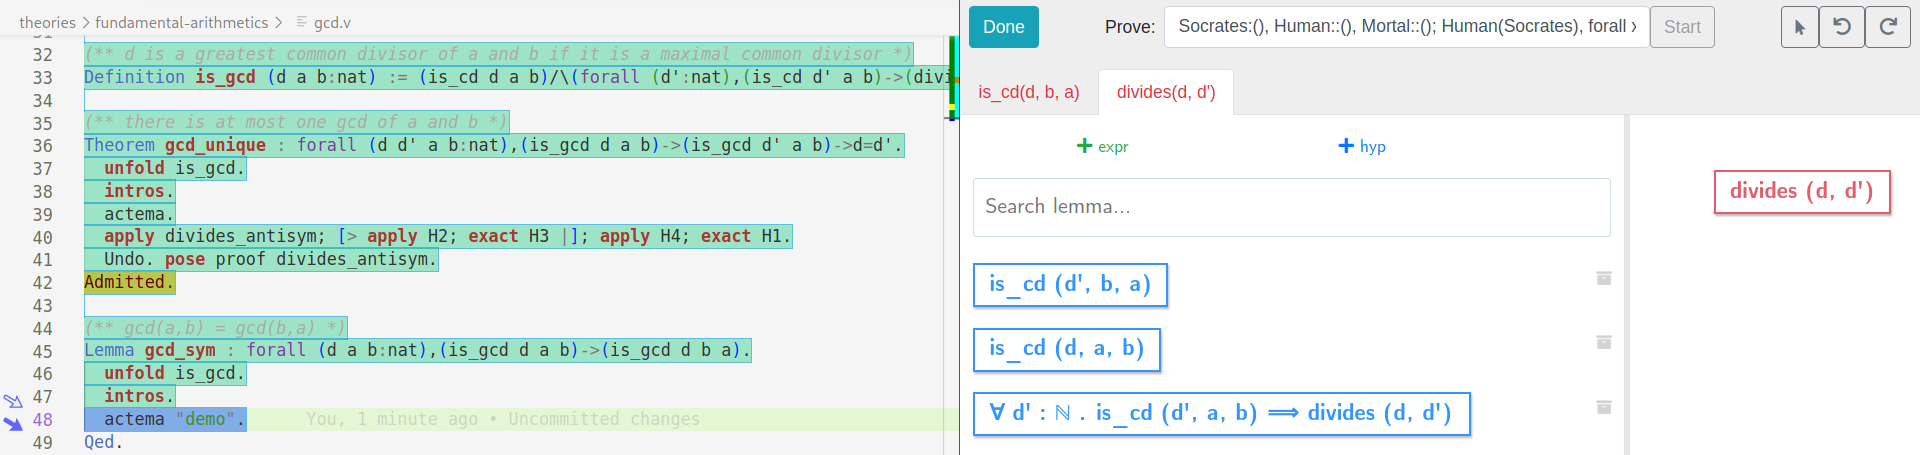
\includegraphics[width=1.5\textwidth]{coq-actema.png}
  \caption{ A possible graphical layout of the \kl{coq-actema} system. On
    the left, the usual interactive view of the \kl{proof script}, in the VsCoq IDE.
    On the right, the graphical \kl{proof view} of \kl{Actema}.}
  \labfig{coq-actema}
\end{figure*}

\begin{figure*}
  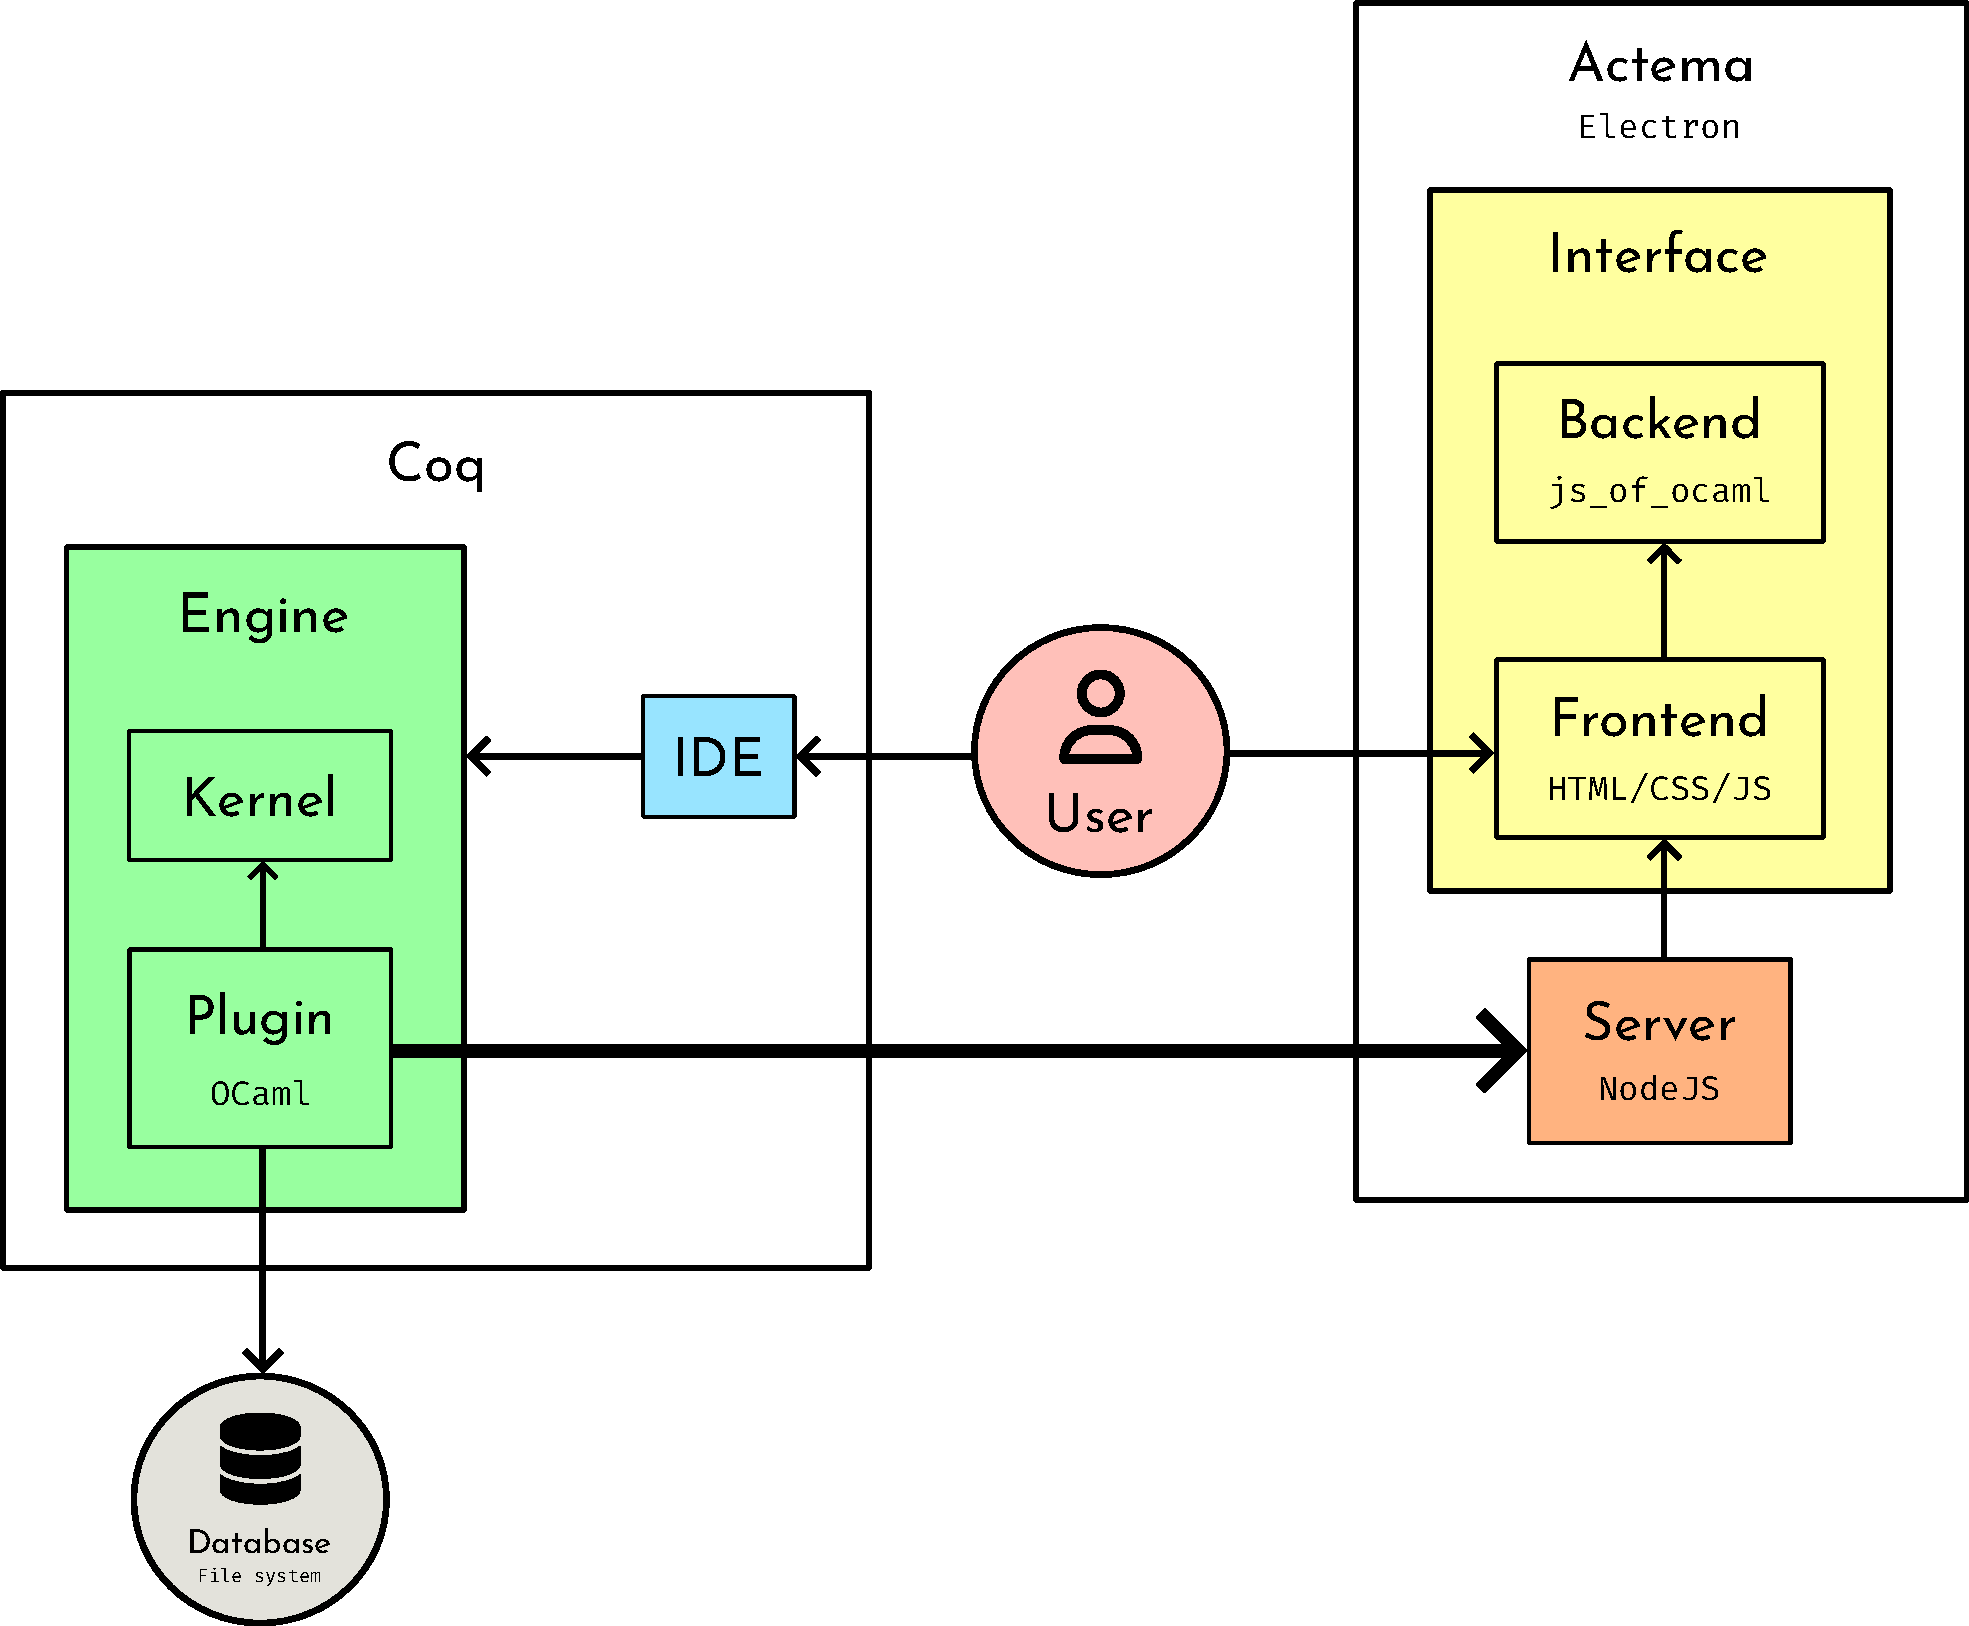
\includegraphics[width=1.3\textwidth]{archi.pdf}
  \caption{Architecture of the \kl{coq-actema} system}
  \labfig{archi}
\end{figure*}

\todo{ Add link to GitHub repository of coq-actema (which should thus become
  public)}

Let us now give the full picture of the \kl{coq-actema} system that
integrates both \kl{Actema} and the \kl{Coq} plugin. A schematic view of its overall
architecture, including the various components and their relationships, is
provided in \reffig{archi}. The different \emph{processes/agents} involved are
represented by shapes of different \emph{colors}, and we add a directed
\emph{arrow} whenever two of them communicate with each other, where the
\emph{source} requests data from, or sends instructions to the \emph{target}.

The \process{User} (pink circle) is the only human agent in the system, and
drives all interactions. She interacts with the \kl{Coq} and \kl{Actema} subsystems
(transparent rectangles), through the interfaces provided by her Coq
\process{IDE} of choice (blue rectangle) and \kl{Actema}'s \process{Frontend} (yellow
rectangle). This will typically take the form of a two-windows layout, as
depicted by the screenshot of \reffig{coq-actema}.

\subsection{Actema web app}

The \kl{Actema} web app runs in a process independent from \kl{Coq}, represented by the
yellow \process{Interface} rectangle. We add a third layer to the
\process{Frontend} and \process{Backend} described in \refsec{actema}, namely a
HTTP \process{Server} (orange rectangle) that handles requests from, and
responses to the \kl{Coq} \process{Plugin}. Thus we implement interprocess
communication between \kl{Actema} and \kl{Coq} through the network layer of the operating
system, rather than a more local mechanism such as Unix pipelines. There are a
few reasons behind our choice of the HTTP protocol:
\begin{itemize}
  \item it provides useful abstractions when working with a client/server
    architecture structured around requests;
  \item it is a widely spread standard, especially in web technologies. Thus we
    were able to reduce development time by reusing generic implementations of
    both client and server from standard libraries;
  \item more anecdotically, this makes it easy to run \kl{Coq} and \kl{Actema} on
    different machines connected on the same network. This could be used for
    instance to offload heavy computations in a proof to the machine running
    \kl{Coq}, while still being able to interact with \kl{Coq} through \kl{Actema} on the
    weaker machine.
\end{itemize}
The \process{Server} runs in a process separate from the \process{Interface}, in
order to avoid any delay in the latter. Then we bundle everything in an Electron
application \sidecite{Electron}, so that \kl{Actema} can easily be run locally on
most operating systems. This also allows us to exploit the multi-process
architecture of Electron \sidecite{ElectronProcess}, where the so-called
\emph{main} process runs the server and has the ability to issue system calls
for networking through the Node.js HTTP library \sidecite{NodeJS}; and the
so-called \emph{renderer} process runs the \process{Interface} in the Chromium
browser.

\subsection{\kl{Coq} plugin}

The \process{Plugin} is loaded dynamically in \kl{Coq}'s \process{Engine} (green
rectangle) by executing the following command in a \kl{proof script}:
\begin{minted}[fontsize=\normalsize]{coq}
  From Actema Require Import Loader.
\end{minted}
% This can be done dynamically by the \process{User} in her \process{IDE}, or
% statically at compile time.
It essentially exposes a single \kl{tactic} called \texttt{actema}, which can run in
two distinct modes:
\begin{description}
  \item[\bfseries Interactive] The \process{Plugin} sends the current \kl{subgoal}s
  to \kl{Actema}, and the user applies a sequence of actions on them. Each time an
  action is performed, it is sent back to \kl{Coq}, compiled into the appropriate
  \kl{tactic} call, and then executed to generate new \kl{subgoals} that are sent again to
  \kl{Actema}. The \texttt{actema} \kl{tactic} finishes its execution either when:
  \begin{itemize}
    \item all \kl{subgoals} are proved (in \kl{Actema});
    \item the \process{User} decides to stop and give back control to the
    \process{IDE};
    \item in some rare cases, an unrecoverable error occurs.
  \end{itemize}

  \item[\bfseries Non-interactive] If the \texttt{actema} \kl{tactic} has already
  been executed on the \kl{subgoal} under focus, then the \process{Plugin}
  automatically saved the sequence of actions performed by the \process{User} in
  a \process{Database} (gray circle). Currently for ease of development, the
  \process{Database} is implemented as a simple directory on the local
  filesystem, where each file encodes an entry as follows:
  \begin{itemize}
    \item the filename is a hash code that uniquely identifies the \kl{goal} by both
    its \emph{content}, i.e. the statements of the hypotheses and conclusion,
    and an optional \emph{identifier}, which can be given as argument to the
    \kl{tactic} in the form of an arbitrary string;
    \item the contents of the file is essentially a Base64 encoding of the data
    specifying each action, whose format will be detailed in
    \refsec{compilation}.
  \end{itemize}
  Then the \kl{tactic} will load the sequence of actions from the appropriate file,
  recompile it into one big \kl{tactic}, and execute it on the current \kl{subgoal}.
\end{description}
One can also force the execution in interactive mode by using a variant of the
tactic named \texttt{actema\_force}. We provide details of the complete
interaction protocol followed by the \texttt{actema} \kl{tactic} in the following
section.

Regarding the implementation of the \process{Plugin}, we chose to do it in the
standard way by interfacing with the \texttt{coq-core} API in OCaml
\sidecite{CoqCore}, although it has been encouraged in recent versions of \kl{Coq} to
interface with more stable APIs such as those provided by \kl{Coq}-Elpi
\sidecite{CoqELPI} and MetaCoq \sidecite{MetaCoq}\sidenote{Indeed breaking
changes are frequently introduced in \texttt{coq-core} with newer versions of
\kl{Coq}, which requires more maintenance efforts from plugin developers.}. The main
reason is that our plugin performs \emph{side effects} by interacting with an
external environment: the file system when saving and retrieving graphical
proofs, and the network when issueing HTTP requests to \kl{Actema}. Those cannot be
implemented in the aforementioned frameworks.

\section{Interaction protocol}\labsec{protocol}

\begin{figure*}
  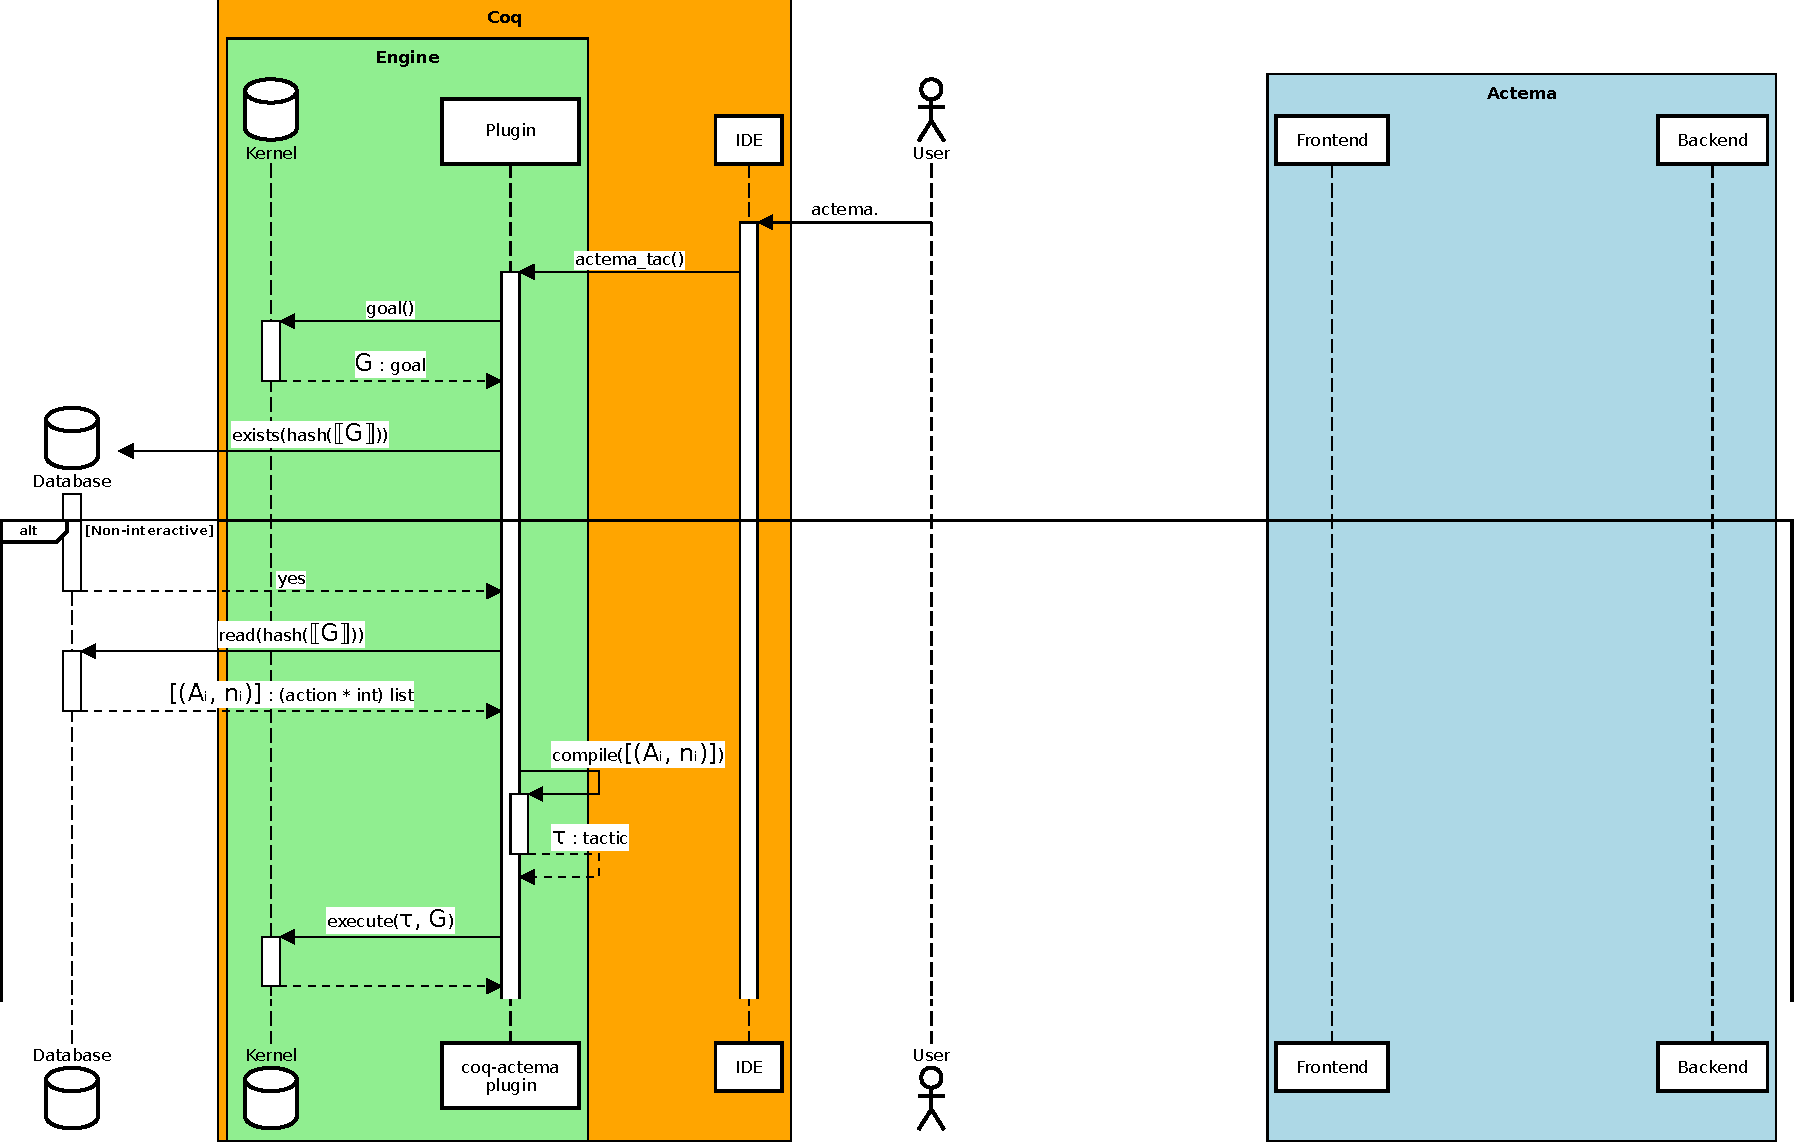
\includegraphics[angle=90,height=\textheight]{protocol-1.pdf}
  \vspace{2em}
  \caption{Sequence diagram of \kl{coq-actema}'s interaction protocol ---
  non-interactive mode}
  \labfig{protocol1}
\end{figure*}

\begin{figure*}
  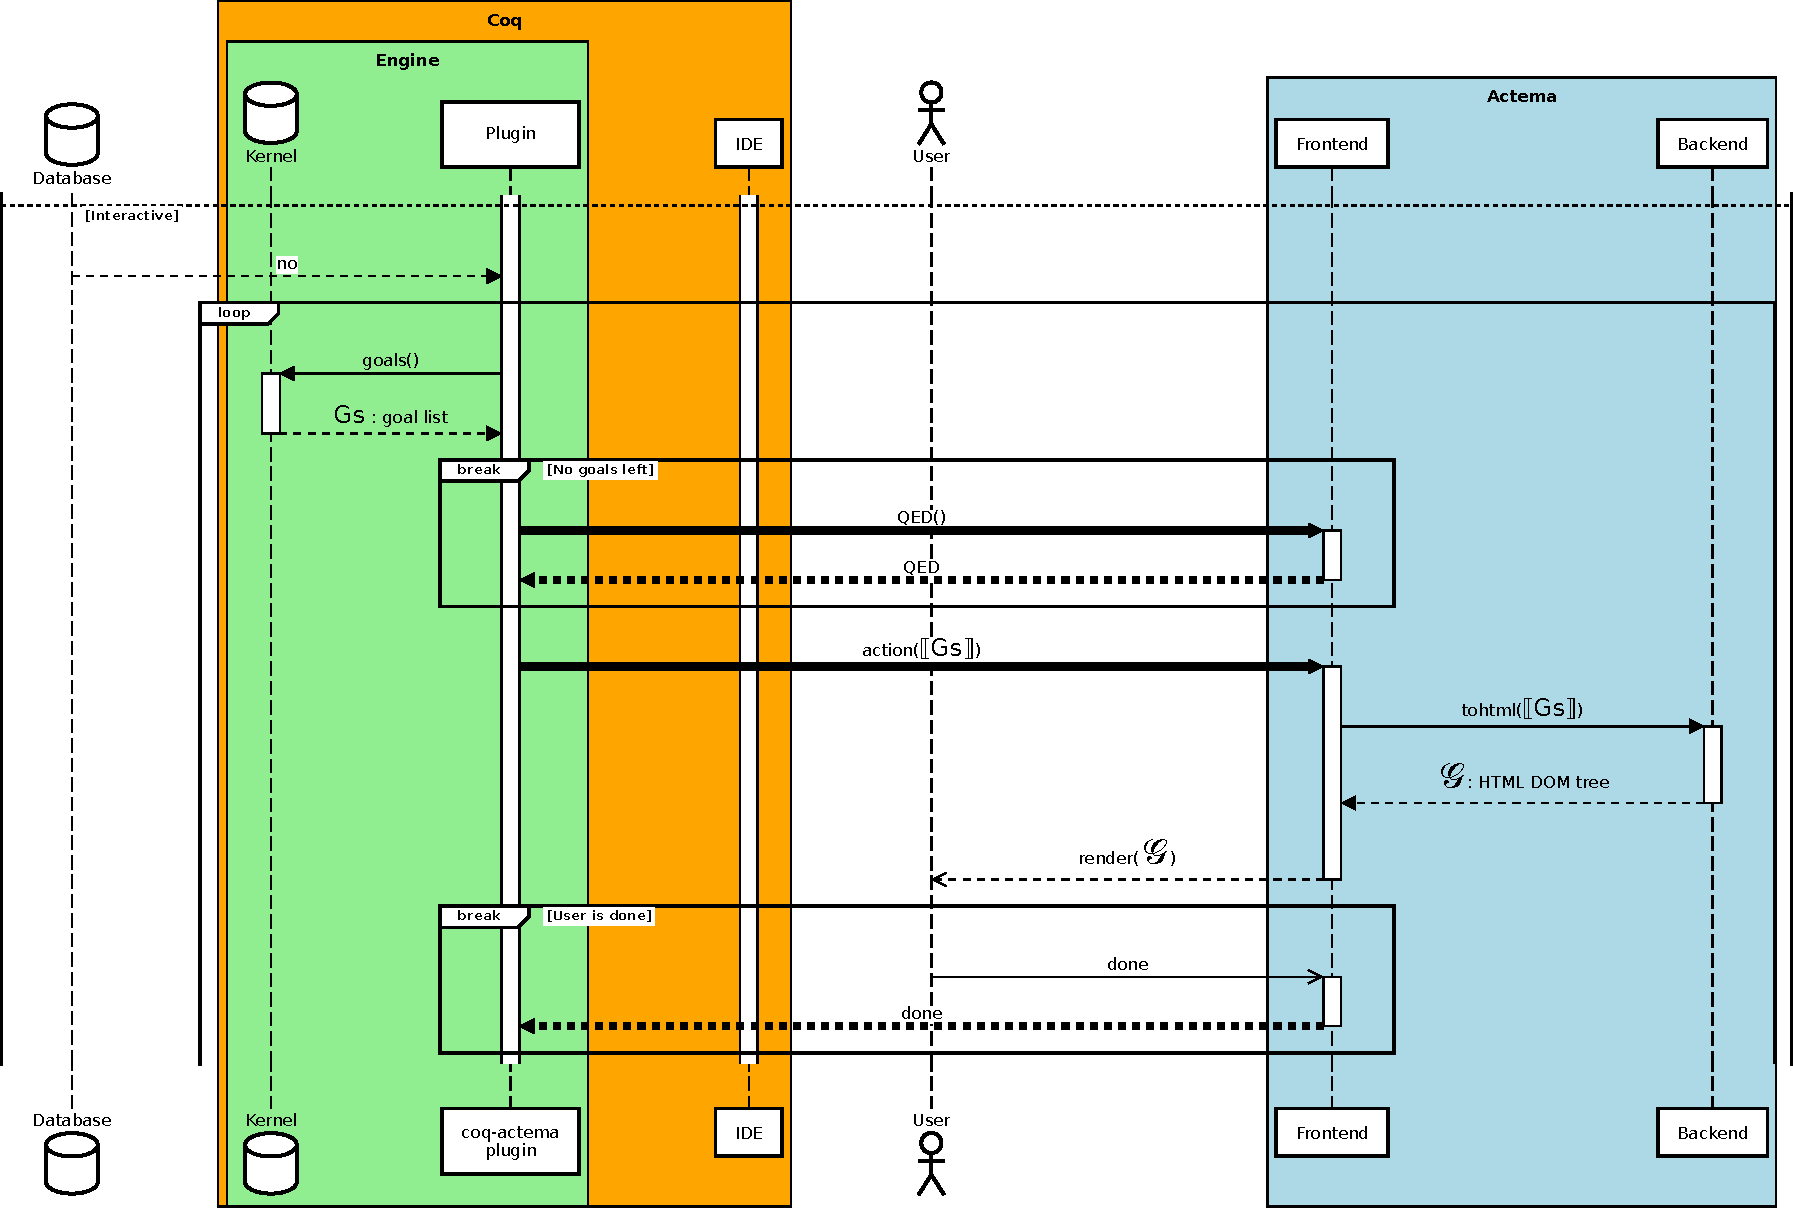
\includegraphics[angle=90,height=\textheight]{protocol-2.pdf}
  \vspace{2em}
  \caption{Sequence diagram of \kl{coq-actema}'s interaction protocol ---
    breaking out of the interaction loop}
  \labfig{protocol2}
\end{figure*}

\begin{figure*}
  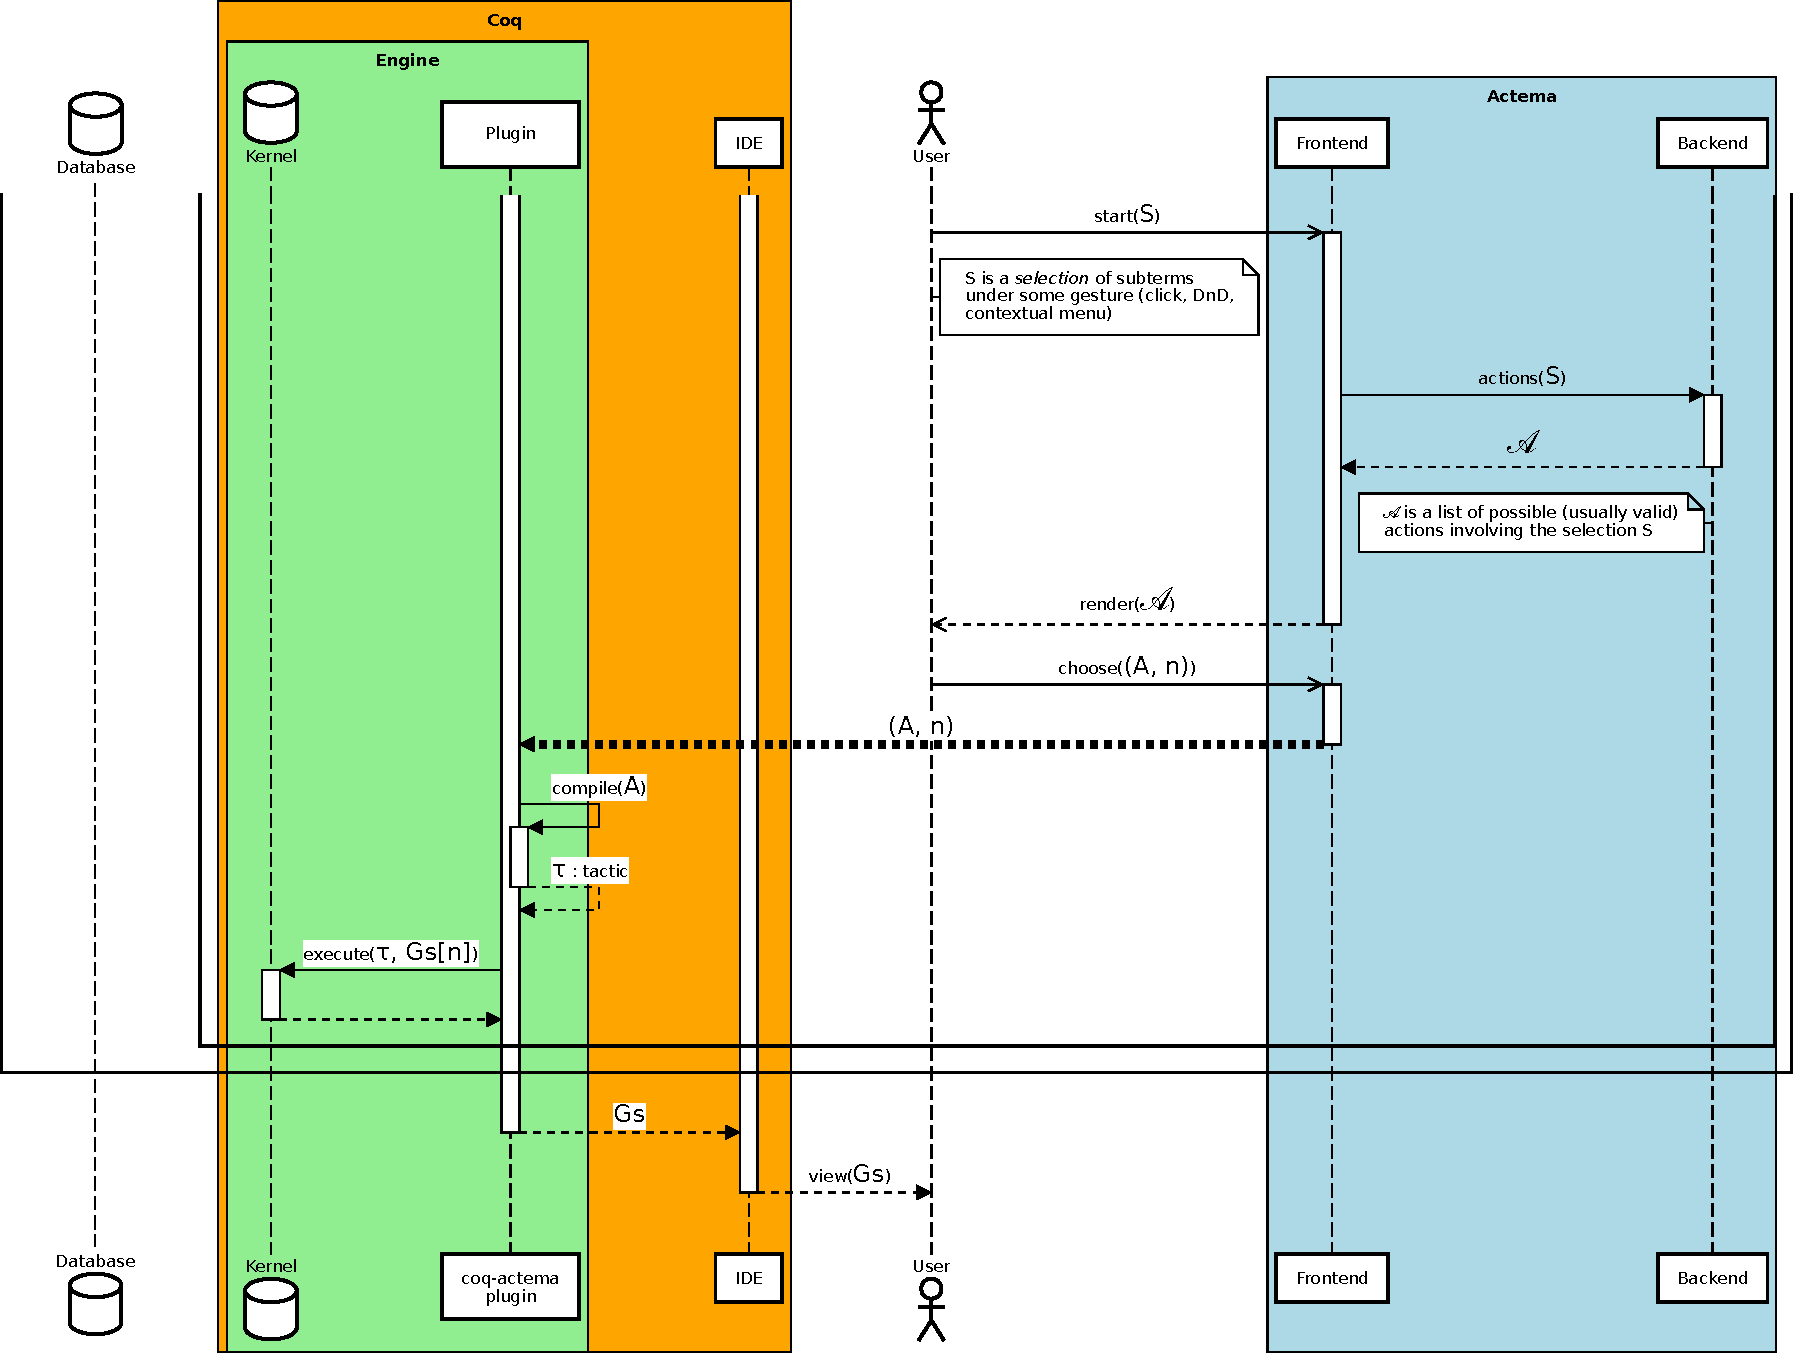
\includegraphics[angle=90,height=0.9\textheight]{protocol-3.pdf}
  \vspace{2em}
  \caption{Sequence diagram of \kl{coq-actema}'s interaction protocol ---
    applying an action}
  \labfig{protocol3}
\end{figure*}

We will now unroll the details of a complete interaction in \kl{coq-actema},
starting from the \process{User} calling the \texttt{actema} \kl{tactic} in her
\process{IDE}, and ending with her viewing the new \kl{subgoals} displayed in the
\process{IDE}. We chose to represent this with a \emph{sequence diagram}, as
specified by the UML standard \cite{enwiki:1153944336}. This kind of \kl{diagram} is
used to depict runtime behavior of a system, showing interactions between
objects and the messages they exchange in the order they occur chronologically.
In our case, the objects are the different processes described in the previous
section, as well as the \process{User}. Since the full interaction is quite
involved, we split the \kl{diagram} in three parts: \reffig{protocol1} includes the
beginning of the interaction, focusing on the non-interactive mode of the
\texttt{actema} \kl{tactic} where the \process{Plugin} communicates with \kl{Coq}'s
\kl(PA){kernel} and the \process{Database}. \reffig{protocol2} and
\reffig{protocol3} tackle the interactive mode of the \texttt{actema} \kl{tactic}:
\reffig{protocol2} focuses on the conditions for breaking out of the interaction
loop, and \reffig{protocol3} on the interactions at work when the \process{User}
performs a proof action in \kl{Actema}.

\subsection{Translating goals}

The first task performed by the \process{Plugin} when calling the
\texttt{actema} \kl{tactic} is to ask the \kl(PA){kernel} for the data of the \kl{subgoal} $G$
currently under focus. Then for the \kl{goal} $G$ to be understandable by the
\process{Backend} of \kl{Actema}, the \process{Plugin} will translate it into a new
representation $\trgoal{G}$ in a custom datatype. In order to share the
definition of this datatype across implementations of the \process{Plugin} and
\process{Backend}, we decided to use the ATD data specification language
\cite{ATD}. It provides a set of tools to automatically generate idiomatic
datatype definitions in a few target languages --- including OCaml --- along
with (de)serialization and validation helpers. This is particularly fit for our
usecase, where we need to serialize complex data like $\trgoal{G}$ in order to
transmit it over HTTP messages. Since both the \process{Plugin} and
\process{Backend} are written in OCaml, it also allows us to share across
implementations our own domain-specific helpers for manipulating this data.

\begin{figure}
  \begin{minted}
  [
  frame=lines,
  framesep=2mm,
  baselinestretch=1,
  fontsize=\footnotesize,
  linenos
  ]
  {ocaml}

(* -------------------------------------------------------------------- *)
(** Identifiers *)

type name = string

(* -------------------------------------------------------------------- *)
(** Types *)

type type_ = [
  | TVar of name
]

type arity = type_ list
type sig_  = (arity * type_)

(* -------------------------------------------------------------------- *)
(** Expressions *)

type expr = [
  | EVar of name
  | EFun of (name * expr list)
]

(* -------------------------------------------------------------------- *)
(** Formulas *)

type logcon = [ And | Or | Imp | Equiv | Not ]
type bkind  = [ Forall | Exist ]

type form = [
  | FTrue
  | FFalse
  | FPred of (name * expr list)
  | FConn of (logcon * form list)
  | FBind of (bkind * name * type_ * form)
]

(* -------------------------------------------------------------------- *)
(** Terms = Formulas + Expressions *)

type term = [F of form | E of expr]

(* -------------------------------------------------------------------- *)
(** Environments *)

(* Body of a variable declaration, holding its type and eventually an expression
    in the case of a local definition *)
type bvar = (type_ * expr option)

type varenv = (name * bvar) list

type env = {
  env_sort      : name                       list; (* Sorts, i.e. atomic types *)
  env_prp       : (name * arity            ) list; (* Predicate symbols *)
  env_fun       : (name * sig_             ) list; (* Function symbols *)
  env_sort_name : (name * name             ) list;
  env_prp_name  : (name * name             ) list;
  env_fun_name  : (name * name             ) list;
  env_var       : varenv;                          (* Variable declarations *)
}

(* Local environment, only maps abstract variables to their type *)
type lenv = (name * type_) list 

\end{minted}

  \caption{ATD definitions for \kl{first-order} formulas and environments}
  \labfig{atd-fo}
\end{figure}

\begin{figure}
  \begin{minted}
  [
  frame=lines,
  framesep=2mm,
  baselinestretch=1,
  fontsize=\footnotesize,
  linenos
  ]
  {ocaml}

(* -------------------------------------------------------------------- *)
(** Goals *)

(* Unique identifier *)
type uid = string

(* Hypothesis *)
type hyp = {
  h_id : uid;
  h_form : form;
}

(* Goal *)
type goal = {
  g_env : env;
  g_hyps : hyp list;
  g_concl : form;
}

type goals = goal list

(* Abstract goal, without the signature *)
type agoal = {
  a_vars : varenv;
  a_hyps : hyp list;
  a_concl : form;
}

\end{minted}

  \caption{ATD definitions for \kl{goals}}
  \labfig{atd-goals}
\end{figure}

The ATD definition of \kl{goals} is given by the \texttt{goal} type in
\reffig{atd-goals}\sidenote{The syntax is almost the same as that of OCaml
datatypes, for the reader already acquainted with this language.}. It relies on
the ATD types \texttt{form} of \emph{formulas}, and \texttt{env} of
\emph{environments} of available constants and variables. In our setting, these
correspond respectively to the formulas and \emph{signatures} of many-sorted
\kl{first-order logic}, whose ATD definitions are given in \reffig{atd-fo}. But one
could imagine using formulas and environments in \kl{higher-order} logic instead, and
this would not change the structure of the \texttt{goal} datatype. Note that
hypotheses are encoded with a \texttt{h\_id} attribute corresponding to their
string identifier in the \kl{Coq} \kl{goal}, even though we do not display it in \kl{Actema}'s
interface. This is required later by the plugin to compile actions into \kl{tactics},
because we need to identify which \kl{Coq} hypotheses correspond to those designated
graphically by the \process{User}.

\subsection{Retrieving actions}

The next step for the \process{Plugin} is to check if there already exists a
graphical proof associated to $\trgoal{G}$ in the \process{Database}. If so,
then it retrieves it in the form of a list $A$ of \emph{actions}, whose data
format will be precised in \refsec{compilation}. There is also a positive
integer $n_i$ associated to each action $A_i$ in the list, corresponding to the
index of the \kl{goal} to which $A_i$ applies in the list of \kl{subgoals}. Then each
$A_i$ is compiled into a \kl{tactic} $\traction{A_i}$, and all the $\traction{A_i}$
are composed into a unique \kl{tactic} $\tau$, which is executed by the
\kl(PA){kernel} on $G$ to apply the full sequence of actions.

\begin{remark}
  Currently the translation $\trgoal{\cdot}$ is not \emph{injective}: it might
  map two different \kl{Coq} \kl{goals} to the same \kl{Actema} \kl{goal}, because strictly
  \kl{higher-order} subterms are translated into a \texttt{dummy} atomic predicate.
  Thus one might retrieve a proof from a different \kl{goal} when calling the
  \texttt{actema} \kl{tactic}. However this is not problematic, since the
  \process{User} cannot perform any actions involving the part of the two goals
  that make them distinct; they might as well be seen as the same \kl{goal} from her
  point of view. It can thus be considered as a feature that maximizes proof
  reuse.
\end{remark}

Otherwise the \texttt{actema} \kl{tactic} has never been executed on $\trgoal{G}$,
and thus we let the \process{User} provide a (partial) proof in \kl{Actema}. First
the \process{Plugin} retrieves the list $Gs$ of all \kl{subgoals}, instead of just
the one under focus. If $Gs$ is empty, which would happen after all subgoals
have been solved from \kl{Actema}, then it sends a \request{QED} request to \kl{Actema} so
that the latter can update its view accordingly, and the interaction loop with
Actema stops here\sidenote{In \reffig{protocol2} and \reffig{protocol3}, we
depict requests as being sent to the \process{Frontend} of \kl{Actema}. This is an
imprecision for trading some readability, since as reviewed in
\refsec{architecture} it is the \process{Server} which handles communication
with the \process{Plugin}, and in particular forwards requests to the
\process{Frontend}.}.

Otherwise there is at least one \kl{subgoal}, and we send an \request{action} HTTP
request to \kl{Actema}, whose body contains the translated \kl{subgoals} $\trgoal{Gs}$. To
do this, we chose to serialize $\trgoal{Gs}$ with the Biniou helpers
autogenerated by atdgen, the OCaml backend of ATD. According to its authors:
``Biniou is a binary format extensible like JSON but more compact and faster to
process'' \sidecite{atdgen}. This data is then deserialized and compiled into a
set $\mathcal{G}$ of HTML DOM nodes by the \process{Backend}, so that the goals
can be rendered by the \process{Frontend} and exposed to the \process{User}.
Then the \process{User} has two options:
\begin{itemize}
  \item she can apply either a click, \kl{DnD} or contextual action\sidenote{See
  \refsec{funcs} for an introductory example of contextual action with
  \action{Unfold}.}. The precise protocol followed for applying an action is
  summarized in \reftab{action-protocol}. Let us focus on the more complex case
  of \kl{DnD} actions. The \textbf{Start} column describes how the \process{User}
  \emph{starts} the action, here by dragging some \kl{item} $I$ of the current
  \kl{subgoal}. Then the \process{Frontend} asks the \process{Backend} for the set
  $\mathcal{A}$ of all available \kl{DnD} actions involving $I$. The
  \textbf{Selection} column describes how the computation of $\mathcal{A}$ is
  impacted by the set $S$ of subterms that are selected in the current \kl{subgoal}.
  For \kl{DnD} actions, we essentially filter out all \kl{linkages} that do not match the
  selection. The \textbf{Render} column describes how $\mathcal{A}$ is
  \emph{rendered} to the \process{User}: here we highlight all valid drop
  targets, which correspond to subterms of the current \kl{goal} located in other
  \kl{items}\sidenote{Highlighting is here understood in a \emph{visual} sense: in
  the current implementation of \kl{Actema}, subterms are indicated graphically by
  squaring them. But one could imagine other modalities for highlighting,
  typically \emph{spelling} the subterms with a speech synthesis algorithm for
  users with impaired vision.}. Lastly, the \textbf{End} column describes how
  the user chooses a specific action $A \in \mathcal{A}$ to apply, here by
  dropping $I$ on a given target. Then $A$ is serialized and sent in the body of
  the response to the \request{action} request, together with the index $n$ of
  the \kl{subgoal} under focus in \kl{Actema}. The \process{Plugin} can therefore compile
  $A$ into a \kl{tactic} $\traction{A}$ which is executed on the $n^{\text{th}}$ Coq
  \kl{subgoal}, giving a new list of \kl{subgoals} which is sent again to \kl{Actema} for
  another round of the interaction loop.

  \item or she can click on a \texttt{Done} button in \kl{Actema}'s interface: this
  has the effect of answering the \request{action} request from the
  \process{Plugin} with a \request{done} response, and the interaction loop with
  \kl{Actema} stops here. This will happen when the \process{User} wants to go back
  to editing the \kl{proof script}, either because she is satisfied with the new
  \kl{subgoals} obtained from previous actions, or because she is stuck and wants to
  try native \kl{Coq} \kl{tactics} instead. Indeed our protocol is \emph{synchronous}: the
  \process{IDE}'s interface is stuck until the \texttt{actema} \kl{tactic} has
  finished its execution, and thus one cannot edit the \kl{proof script} \emph{and}
  build a proof in \kl{Actema} at the same time.
  % \sidenote{This is because the
  % \emph{document checking model} of most \kl{Coq} IDEs is itself synchronous: when
  % the \process{User} modifies the \kl{proof script} at a location before the current
  % execution point, the proof state goes back to how it was at that location, and
  % every command/tactic coming after it needs to be reinterpreted.}
\end{itemize}

\begin{table*}[]
  \def\arraystretch{1.5}
  \begin{tabular}{|c|C{0.2\textwidth}|C{0.4\textwidth}|C{0.25\textwidth}|C{0.2\textwidth}|}
  \hline
  \textbf{Kind} & \textbf{Start}       & \textbf{Selection $S$} &
  \textbf{Render}                      & \textbf{End} \\ \hline
  Click         & Hover \kl{item} $I$       & Ignored & Highlight $P \subseteq
  \subterms{I}$ & Click on some $p \in P$    \\ \hline
  \kl{DnD}           & Drag \kl{item} $I$        &
      If $\exists p \in S \cap \subterms{I}$ then match only $p \link q$ where
      $q \in \compl{\subterms{I}}$
      \newline
      If $\exists q \in S \cap \compl{\subterms{I}}$ then match only $p
      \link q$ where $p \in \subterms{I}$
    & Highlight $Q \subseteq \compl{\subterms{I}}$ & Drop on some $q \in Q$ \\ \hline
  Contextual    & Open menu & Populate menu only with actions
  applicable on $S$ & Show menu & Choose an \kl{item} in the menu \\ \hline
  \end{tabular}
  \raggedright
  \parbox{\textwidth}{
    \vspace{1.5em}
    We introduced some notations for conciseness:
    \begin{itemize}
      \item $p, q$ denote paths to subterms of the current goal
      \item $P, Q$ and the selection $S$ denote sets of paths
      \item $\subterms{I}$ denotes the set of paths within \kl{item} $I$
      \item $\compl{\subterms{I}}$ denotes the complement of $\subterms{I}$, i.e.
      all paths in all \kl{items} $J \not= I$
      \item $p @ q$ is a \kl{linkage} as introduced in \refsec{linkages}
    \end{itemize}}

  \caption{Protocol for applying an action in Actema}
  \labtab{action-protocol}
\end{table*}


\section{Compiling actions}\labsec{compilation}

Once it has received the actions to execute, either from the \process{Database}
or the \process{User}, the \process{Plugin} will compile them with a function
$\traction{\cdot}$ which translates any action $A$ into a \kl{Coq} tactic
$\traction{A}$. This function actually has access to some other data used for
interpreting actions: \kl{Coq}'s \kl{goal} $G$, its \kl{Actema} translation $\trgoal{G}$, and a
bijective mapping $\Sigma$ between \kl{Coq} constants in the environment of $G$ and
the corresponding \kl{Actema} symbols in the \kl{first-order} signature of $\trgoal{G}$.

\subsection{The \texttt{action} datatype}

\begin{figure}
  \begin{minted}
  [
  frame=lines,
  framesep=2mm,
  baselinestretch=1,
  fontsize=\footnotesize,
  linenos
  ]
  {ocaml}
  
(* -------------------------------------------------------------------- *)
(** Actions *)

(* A path refers to a subterm in the current subgoal, through a [handle]
    identifying an item of kind [kind], and a list of integers [sub] designating
    the specific subterm of the item *)
type pkind = [Hyp | Concl | Var of [Head | Body]]
type ctxt = { kind : pkind; handle : uid }
type ipath = { ctxt : ctxt; sub : int list }

(* Trace of a subformula linking, from which the list of rewrite rules to apply
   can be reconstructed *)
type choice = (int * (lenv * lenv * expr) option)
type itrace = choice list

type action = [
  | AId                                     (* The empty action which does nothing *)
  | ADef of (name * type_ * expr)           (* Introduction of a local definition *)
  | AIntro of (int * (expr * type_) option) (* Click on a conclusion *)
  | AExact of uid                           (* Proof by assumption *)
  | AElim of (uid * int)                    (* Click on a hypothesis *)
  | AInd of uid                             (* Click on a variable of inductive type *)
  | ASimpl of ipath                         (* Simplify contextual action *)
  | ARed of ipath                           (* Unfold contextual action *)
  | AIndt of ipath                          (* Induction contextual action *)
  | APbp of ipath                           (* Proof-by-Pointing contextual action *)
  | ACase of ipath                          (* Case contextual action *)
  | ACut of form                            (* Click on +hyp button *)
  | AGeneralize of uid                      (* Generalization of a hypothesis *)
  | AMove of (uid * uid option)             (* Reordering of a hypothesis *)
  | ADuplicate of uid                       (* Duplication of a hypothesis *)
  | ALink of (ipath * ipath * itrace)       (* DnD action for subformula linking *)
  | AInstantiate of (expr * ipath)          (* DnD action for instantiating a quantifier *)
]

(* An action identifier is a pair of an abstract goal and an arbitrary string identifier *)
type aident = (string * agoal)

\end{minted}

  \caption{ATD definitions for actions}
  \labfig{atd-actions}
\end{figure}

The \texttt{action} datatype is described thoroughly in the ATD specification
provided in \reffig{atd-actions}. It is a big algebraic datatype, where each
constructor encodes a specific \emph{type} of action. An action's type is
equivalent to the \emph{signature} of a \kl{tactic}, i.e. its name and the types of
its arguments. In particular, the translation function $\traction{\cdot}$ is
defined as a big pattern-matching on the action's type\sidenote{Note that an
action's type is orthogonal to what we referred to as its \emph{kind} in
\reftab{action-protocol}, that is the interface mechanism through which it is
accessible. One might for example want to map some action types to \emph{vocal
commands} instead of click or \kl{DnD} gestures.}. The arguments in action types rely
on most datatypes defined previously in \reffig{atd-fo} and \reffig{atd-goals},
and on two new datatypes: the type \texttt{ipath} of \emph{paths}, which is used
pervasively to designate subterms of the current \kl{subgoal} (that are typically
indicated by the \process{User} through pointing); and the type \texttt{itrace}
of \emph{\kl{subformula linking} traces}, which is used in the compilation of \kl{DnD}
actions that perform \kl{subformula linking}, to be described soon.

Most click and contextual actions have a straightforward translation as Coq
tactics. For instance, the \texttt{AIntro} action that corresponds to a click on
the conclusion $C$ will be mapped to the \kl{Coq} \kl{tactic} that introduces the main
connective of $C$, and is thus defined by case on the latter: \texttt{intro} for
$\limp$ and $\forall$, \texttt{split} for $\land$, etc. The actions
\texttt{AInd}, \texttt{ASimpl} and \texttt{ARed} correspond respectively to the
contextual actions \action{Induction}, \action{Simplify} and \action{Unfold}
introduced in \refch{advanced}, and are mapped almost directly to the equivalent
\kl{Coq} \kl{tactics} \texttt{induction}, \texttt{simpl} and \texttt{red}. The only
difference is that they have a \emph{\kl{deep inference}} flavor, since they can all
be applied on an arbitrary subterm selected by the \process{User}. This relies
on our implementation of \kl{deep inference} semantics directly in \kl{Coq}, that we now
briefly describe.

\subsection{Deep inference semantics}

In a \kl{deep inference} setting, one can reason on subterms located arbitrarily
\emph{deep} inside statements, usually by applying some kind of \kl{rewriting
rules} on them. In particular, the semantics of \kl{DnD} actions described in
\refch{sfl} are based on the rules of SFL (\reffig{DISL}). To implement them, we
chose to do a \emph{deep embedding} of \kl{first-order logic} inside \kl{CoIC}.
Here the word ``deep'' has a different meaning, related to the fact that we
encode the statements of \kl{first-order logic} with our own custom datatypes,
instead of reusing the statements of \kl{CoIC}. This makes it easier to define
the SFL \kl{rewriting rules}, in particular because we need to manipulate
\emph{\kl{contexts}} (\refdef{formula-context}) explicitly, and those are
not available for \kl{CoIC} propositions.

Then we use a technique called \emph{computational reflection} in order to apply
the embedded \kl{deep inference} semantics to \kl{Coq} \kl{goals}. Originating from the
\emph{small scale reflection} methodology supported by the {\kl{\ssreflect}}
framework \cite{SSR}, it consists in translating \kl{Coq} objects into their
equivalent formulation in the deep embedding with a \texttt{reify} function,
reasoning on the deep embedding with \kl{Coq} programs (also called
\emph{fixpoints}), and then translating objects back into \kl{Coq} with a
\texttt{reflect} function. It is easy to implement the \texttt{reflect} function
because the datatypes in a deep embedding are almost always defined as
\emph{inductive} \kl{types}, and thus one can easily do pattern-matching on them. It
is a different story for the \texttt{reify} function, especially in our case:
indeed we want to translate the statements of \kl{Coq} \kl{goals} into \kl{first-order}
propositions. But \kl{Coq} statements are objects of \kl{type} \texttt{Prop}, and thus
cannot be pattern-matched on inside \kl{CoIC}\sidenote{For reasons of
\kl{consistency} of the logic, well-known in the literature on \kl{type theory}.}.
Thus we need to have recourse to a \emph{meta-programming} language in order to
inspect the structure of \kl{Coq} \kl{goals}. Here we use the standard {\ltac} language,
which provides powerful constructs for pattern-matching on \kl{goals}\sidenote{A
downside of {\ltac} is that it is an \emph{untyped} language, whose programs are
notoriously hard to debug and maintain. One might consider a cleaner
implementation with more recent alternatives in the \kl{Coq} ecosystem, like the
successor to {\ltac} Ltac2 \cite{Ltac2}, or the MetaCoq project
\cite{MetaCoq}.}.

The most complex \kl{tactics} are those implementing \kl(dnd){backward} and \kl(dnd){forward} \kl{DnD}
actions, called respectively \texttt{backward} and \texttt{forward}. They rely
on two \kl{Coq} fixpoints \texttt{b3} and \texttt{f3} which respectively compute the
new conclusion $\mathtt{b3}(p, q, T)$ from a \kl(dnd){backward} \kl{linkage} $p \back q$, and
the new hypothesis $\mathtt{f3}(p, q, T)$ from a \kl(dnd){forward} \kl{linkage} $p \forw q$,
where $T$ is the so-called \emph{\kl{subformula linking} trace} mentioned earlier. Of
course the paths $p, q$ and the trace $T$ are all expressed with custom Coq
datatypes relying on our deep embedding of \kl{first-order logic}. The role of the
trace in particular is to provide the list of SFL \kl{rewriting rules} to apply,
including \kl{Coq} \kl{terms} instantiating quantifiers that were computed in \kl{Actema} by
\kl{unification} of the two linked subformulas. Then we formulate in \kl{Coq} two theorems
that guarantee the logical \emph{soundness} of \texttt{b3} and \texttt{f3}
(\reffig{dnd-snd}). Note that the theorems are formulated using the native
implication connective \texttt{->} of \kl{Coq}, thanks to the \texttt{reflect}
function. The final \kl{tactics} \texttt{backward} and \texttt{forward} can thus
modify the \kl{goal} by simply applying these theorems, first reifying the \kl{goal} with
the \texttt{reify} function, and then relying on the fact (also proved in \kl{Coq})
that \texttt{reflect} is the inverse of \texttt{reify}.

\begin{figure}
  \begin{minted}
  [
  frame=lines,
  framesep=2mm,
  baselinestretch=1,
  fontsize=\footnotesize,
  linenos
  ]
  {coq}

Theorem b3_corr : forall p q T,
  coerce p -> coerce (b3 p q T) -> coerce q.

Theorem f3_corr : forall p q T,
  coerce p -> coerce q -> coerce (f3 p q T).

\end{minted}

  \caption{Soundness theorems of \kl{DnD} fixpoints in \kl{Coq}}
  \labfig{dnd-snd}
\end{figure}

% \begin{theorem}[Soundness of \kl{DnD} fixpoints]~\\
%   $$\forall p.\ \forall q.\ \forall T.\ \mathtt{reflect}(p) \limp
%   \mathtt{reflect}(\mathtt{b3}(p, q, T)) \limp \mathtt{reflect}(q)$$
%   \center{and}
%   $$\forall p.\ \forall q.\ \forall T.\ \mathtt{reflect}(p) \limp
%   \mathtt{reflect}(q) \limp \mathtt{reflect}(\mathtt{f3}(p, q, T))$$
% \end{theorem}

\begin{remark}
  There exist a few other approaches to the computer implementation of \kl{deep
  inference} systems. Ozan Kahramanoğulları has pioneered the field, by
  implementing various \kl{calculi of structures} inside frameworks like Maude
  \cite{kahramanogullari_maude_2008} and Tom
  \cite{kahramanogullari_implementing_2005}, that are dedicated to the
  specification of \kl{rewriting systems}. For an integration within modern
  \kl{proof assistants}, we only know of Chaudhuri's recent work
  \sidecite{chaudhuri_certifying_2022} that explores different techniques in
  addition to reflection, like \emph{combinators} and some more powerful usages
  of \emph{metaprogramming}. He also provides an effective implementation of the
  techniques in his \kl{Profint} tool \cite{DBLP:conf/cade/Chaudhuri21}, that
  allows to export \kl{subformula linking} derivations built with \kl{Profint}'s
  \kl{GUI} as \kl{proof scripts} directly executable in various \kl{proof
  assistants} (\kl{Coq}, \kl{Lean}, \kl{Isabelle/HOL}).
\end{remark}

\section{Future works}\labsec{pluginfuture}

The \kl{coq-actema} system described in this chapter has been successfully
implemented and tested on various simple examples, including those of
\refsec{edukera} and \refsec{arith}. But there are many \kl{Coq} \kl{goals} that cannot be
properly handled in \kl{Actema}, which still hinders the usability of the system in
real mathematical developments, even in an educational setting. Typically, the
example of \refsec{funcs} cannot be completely performed in \kl{Actema}, in this case
because of the lack of support for \emph{\kl{higher-order}} functions and predicates,
but also because of the poor support for user-defined \emph{notations}. Those
are only a few of the current limitations of \kl{coq-actema}, and we
describe in the following pages how they could be overcome, both to widen the
scope and improve the \kl{UX} of the system.

\subsection{Higher-order logic}

The importance of being able to express and manipulate \kl{higher-order} functions
and predicates has been stressed multiple times before. The fact that \kl{Actema} is
limited to \kl{first-order logic} is mostly a historical contingency, motivated by
the fact that some algorithms like \kl{unification} are more tractable in this
setting. But now that we rely on \kl{Coq}'s proof engine, there is no fundamental
reason for maintaining this choice. Because the language of statements is at the
foundation of a logical framework, many other components of a \kl{proof assistant}
will depend on it. Thus the switch to \kl{higher-order} logic should be done as soon
as possible, to limit the amount of refactoring work to perform in the future.
This will require changes to \kl{Actema}'s \process{Backend} and \process{Frontend},
but also to the \kl{Coq} \process{Plugin}\sidenote{The \kl{Coq} theory implementing the
tactics for \kl{deep inference}-based actions already has partial support for
\kl{higher-order} \kl{goals}, thus work remains mostly on the side of the translation
module for \kl{Actema} written in OCaml.} and the ATD datatype definitions enabling
communication between the two.

One central question in the transition to \kl{higher-order} logic is how \kl{unification}
of subterms will be handled. Algorithms in this setting are known to be
incomplete because of undecidability \sidecite{huet_undecidability_1973}, and
their implementation can be very tricky. The most sensible option seems to rely
on the implementation already provided by \kl{Coq}, which is the fruit of years of
development and improvements. But this would require changing the interaction
protocol of \kl{coq-actema}, by allowing the \process{Backend} of \kl{Actema} to
make \kl{unification} requests to the \process{Plugin}. This might be doable without
changing the current client-server architecture, but will probably involve some
intricate design decisions.

A more radical solution would be to replace the \request{actions} request from
the \process{Frontend} to the \process{Backend} by a \texttt{start} response
from the \process{Frontend} to the \process{Plugin}, with the data of the
selection in its body. Then we could completely delegate the computation of
available actions to the \process{Plugin}, allowing us to freely use \kl{Coq}'s
\kl{unification}. This might not be too hard since we should be able to directly
reuse OCaml code from the \process{Backend}, but is a deeper structural change
to the interaction protocol, that makes the \process{Plugin} responsible for an
important part of \kl{Actema}'s behavior. And this would induce a lot of unnecessary
reimplementation efforts if we were to port the \process{Plugin} to other PAs.

\subsection{Notations}

Another big limitation already mentioned in the introduction of this chapter, is
that we do not handle custom \emph{notations} for displaying
terms\sidenote{Apart from expressions in Peano arithmetic, for which we have ad
hoc support.}. It is however a crucial feature for making proofs in a specific
domain tractable, especially in the \kl{PbA} paradigm where one needs to
manipulate directly statements in the \kl{goal}. Now that we are connected to \kl{Coq}, we
can in principle reuse the notation system already implemented within \kl{Coq}. The
\texttt{coq-core} OCaml API indeed exposes methods for pretty-printing \kl{Coq} terms
using their assigned notations. The problem is that these methods only return
\emph{strings}, but in order to manipulate \kl{terms} interactively in \kl{Actema} we also
need access to \emph{trees} mapping their subterm structure to the
pretty-printed string. At the time of writing there is no support for the
latter, but the \kl{Coq} development team informed us that they plan to add it. The
same problem was met by the developers of the ProofWidgets framework in \kl{Lean},
and they had to modify the pretty-printer of \kl{Lean} upstream\sidenote{Section 4.1
of \cite{ayers_graphical_2021}.}.

Once one has support for custom notations displayed in an HTML page, it is
tempting to also allow for arbitrary HTML/JS code, instead of just textual
notations. This opens the space for very rich graphical and interactive
representations of mathematical objects, which could greatly improve the
accessibility of PAs, but also their expert usage by enabling domain-specific
interfaces targetting non-standard methods of reasoning. A typical example is
the \emph{\kl{diagrammatic}} reasoning pervasive in \emph{category theory}, which is
very hard and cumbersome to express as manipulation of logical statements.
Actually a system very similar to \kl{coq-actema} is currently being
developed by Luc Chabassier \cite{LucTalk}, for the very purpose of integrating
\kl{diagrammatic} proofs in category theory to the traditional \kl{proof script} workflow.
One could imagine in the long-term embedding this system as a subsystem of
\kl{coq-actema}, through an advanced protocol for interactive notations.

In fact the ProofWidgets framework mentioned earlier has been designed with this
usecase in mind from the outset. But they rely on a very different architecture
compared to that of \kl{coq-actema}, where the methods generating the
HTML/JS code of pretty-printed \kl{terms} are directly implemented in a DSL embedded
in the meta-programming language of the PA. While this allows easy access to all
meta-programming facilities for manipulating \kl{terms}, this makes their framework
only usable within \kl{Lean}, while \kl{Actema} could in principle be used with any PA
that implements a corresponding plugin (for example with a \texttt{lean-actema}
variant of our system).

\subsection{Lemma search}

We already described in \refsec{funcs} the \emph{lemma search} feature of
Actema. Currently it is implemented only in its standalone version. Adding
support for it in \kl{coq-actema} would require additional efforts compared
to other contextual actions like \action{Induction}. Indeed we do not only need
access to the current \kl{goal}, but also to the full global environment of \kl{Coq} where
lemmas are stored. While in the standalone version we had a toy lemma database
with very few entries, the standard library of \kl{Coq} contains thousands of lemmas.
And to use our selection-based filtering algorithm implemented in \kl{Actema}, we
need to translate the entire library into statements understandable by \kl{Actema}'s
\process{Backend}, and then send it over HTTP. Thus it will be important to
implement some cache mechanism to remember which lemmas have already been
exported to \kl{Actema}'s own database, to avoid recomputing the translation each
time.

% \subsection{Tighter IDE integration}

% Design a new architecture/protocol that supports \emph{continuous, incremental
% document checking} (typically by inserting tactic calls in the \kl{proof script}
% for each action, maybe coq-lsp can do that?)

\subsection{Proof evolution}\labsubsec{proof-evolution}

\AP
An important question when designing a proving environment is how users will be
able to manipulate an \emph{existing} (partial) proof, either one they have
built in the past, one that was built by other people, or a mix of both in a
collaborative context. This is a complex problem spanning various activities
that are involved in the lifecycle of a proof: modifying it while it is being
constructed; reading it for the first time, or many months/years after it was
written; updating it after slight changes to the statement of its theorem;
etc\sidenote{Not very surprisingly, those activities are commonly found in the
context of \emph{programming} environments. Thus one might get insight by
cross-pollinating ideas from both domains, in the spirit of the \kl{Curry-Howard
correspondence} (which also underlies the design of \kl{Coq}).}\sidenote{One might
even argue that thinking about the best way to \emph{represent} a proof leads to
more fundamental questions, that have been much debated both in \kl{proof theory} and
the history and philosophy of mathematics: what is the essence of a proof, seen
as a meta-mathematical object \cite{strasburger-problem-2019}? What are the
roles played by informal and formal proofs, both in the teaching of mathematics,
and the social and scientific practice of mathematicians
\cite{bartzia:hal-04087080}?}.

In the literature and community of people designing \kl{proof assistants}, these
various problematics are generally regrouped under the term of \intro{proof
evolution}. A fundamental remark about the \kl{PbA} paradigm, and thus about the
\kl{coq-actema} system, is that it has not been designed with \kl{proof
evolution} in mind from the outset. Indeed, a proof built with the
\texttt{actema} \kl{tactic} will provide the least possible amount of information in
the \kl{proof script}, since we can just witness the call to that \kl{tactic}. And
currently there are no facilities to visualize the associated sequence of
actions stored in the \process{Database} of graphical proofs.

The first question that should be answered is: how do we represent statically a
sequence of graphical actions, let alone a single action? For a machine
representation, we can just dump the data of the action invokation, and this is
indeed what we do with the \process{Database}. But finding a human-readable
representation that an average user can quickly manipulate and reason about is a
lot more delicate. The most direct way may be to abandon text altogether, and
just replay the action on the interface through a graphical animation. This is
an intrisically temporal and dynamic representation, akin to a mathematician
unfolding her demonstration on the blackboard. One could then imagine an
interface dedicated to the richly-structured navigation inside this sequence of
animations, in the style of an improved video player.

A more conservative solution would be to find a systematic way to translate a
sequence of actions into a proof text. The question of generating
\kl{declarative} proof texts from \kl{imperative} \kl{proof scripts} has already
been explored by some authors, especially in the case of proofs expressed in
natural language\sidenote{See for example section 3.6 of E. Ayers' thesis
\cite{ayers_thesis}. We can also mention ongoing work of Patrick Massot in the
\kl{Lean} \kl{proof assistant} \cite{LeanIPAM}.}. Our hope is that the structure
of proofs in the \kl{PbA} paradigm might be well-suited to the generation of
readable and concise proof texts, thanks notably to the \kl{subformula linking}
semantics of \kl{DnD} actions that exhibit clearly the flow of argumentation.

An even more pragmatic solution, that should be straightforward to implement in
the short-term, consists in inserting \kl{tactic} invokations in the \kl{proof script}
that are in one-to-one correspondence with graphical actions. Since we actually
compile actions into \kl{tactics}, this is in principle easy to implement. However,
there are currently two drawbacks to this approach:
\begin{itemize}
  \item Since most \kl{tactics} are \kl{deep inference}-based, they take as arguments the
  paths to manipulated subterms, in the form of lists of integers. Those are
  hard to read by humans, and very sensible to small changes in the shape of the
  \kl{goal}. This is even worse for the \texttt{backward} and \texttt{forward}
  \kl{tactics}, because they also take as argument the \kl{subformula linking} trace,
  which is a very complex data structure expressed in our deep embedding of
  \kl{first-order logic}, and hence should not leak into the user interface.
  Hopefully, relying on \kl{Coq}'s \kl{unification} instead of \kl{Actema}'s should mitigate
  the complexity of the trace, by removing the need to incorporate full
  substitutions. There is also the possibility of replacing integer-based paths
  by \emph{patterns} in the {\kl{\ssreflect}} language, which are known to be a more
  robust way to designate subterms. But this would require the design of some
  clever algorithm, able to generate patterns that correctly generalize the
  \process{User}'s intent from the sole data of selected paths.

  \item The interaction protocol described in \refsec{protocol} does not provide
  any way to send requests to the \process{IDE}, which would be necessary to
  actually insert the \kl{tactic} invokation at the right location in the \kl{proof
  script}, and this as soon as the action is performed by the \process{User}. A
  ``brutal'' solution would be to reimplement \kl{coq-actema} as an
  extension of a specific IDE, typically VsCoq which is also based on web
  technologies \cite{VsCoq}. But this would require some big implementation
  efforts, in addition to locking the \process{User} into this specific IDE. A
  better option might be to directly interact with a \emph{language server}
  implementing the Language Server Protocol (LSP) \cite{LSP}. The
  \texttt{coq-lsp} project aims to provide such a server for \kl{Coq}, but at the
  time of writing of this thesis does not implement yet all methods of the LSP
  standard. The one that interests us in particular is the
  \texttt{textDocument/codeAction} method, for which support is currently
  planned \cite{coq-lsp-proto}. Then \kl{coq-actema} would stay compatible
  with all IDEs that run \texttt{coq-lsp}.
\end{itemize}

\pagelayout{wide} % No margins
\addpart{Iconic Manipulations}
\pagelayout{margin} % Restore margins

% !TEX root =index.tex
\setchapterpreamble[u]{\margintoc}
\chapter{Asymmetric Bubble Calculus}
\labch{bubbles}

\epigraph{Leibniz sought to make the form of a symbol reflect its content. ``In
signs,'' he wrote, ``one sees an advantage for discovery that is greatest when
they express the exact nature of a thing briefly and, as it were, picture it;
then, indeed, the labor of thought is wonderfully diminished.''}
{\textbf{Frederick Kreiling}, \textit{Leibniz}, Scientific American, May 1968}


We introduce a new kind of \kl{nested sequent} \kl{proof system} dubbed \intro{bubble
calculus}. Inspired by the \emph{membrane} mechanism of the \intro{chemical
abstract machine} (\reintro{\cham}) \sidecite[25em]{berry_chemical_1989},
so-called \intro{bubbles} internalize the notion of \kl{subgoal} inside
\kl{sequents}, rather than through the tree structure induced by traditional
\kl{inference rules}. This allows for a more hierarchical representation of the
\kl{proof state}, where \kl(sequent){contexts} can be shared between different
\kl{subgoals}. In addition to the usual textual syntax, the \kl{bubble calculus}
can be expressed in a graphical syntax, where logical meaning is captured by
\emph{physical} constraints on \kl{diagrammatic} manipulations, instead of
\emph{virtual} restrictions on available \kl{inference rules}.

% We introduce a new kind of nested sequent \kl{proof systems} dubbed \emph{bubble
% calculi}. Inspired by the \emph{membrane} mechanism of the chemical abstract
% machine ({\cham} hereafter) \sidecite[25em]{berry_chemical_1989}, so-called
% \emph{bubbles} internalize the notion of \emph{subgoal} inside sequents, rather
% than through the tree structure induced by \kl{inference rules}. This allows for a
% more hierarchical representation of the proof state, where contexts can be
% shared between different subgoals. In addition to the usual textual syntax,
% bubble calculi can be expressed in a graphical syntax, where logical meaning is
% captured by \emph{physical} constraints on diagrammatic manipulations, instead
% of \emph{virtual} restrictions on available \kl{inference rules}. In the chemical
% metaphor, \emph{intuitionism} is then characterized as the phenomenon of
% \emph{repulsion} between objects that have the same polarity.

We start in \refsec{chemical} with the genesis of the idea of \kl{bubble calculus},
coming from the observation that our \kl{Proof-by-Action} paradigm (\refch{pba})
lends itself quite naturally to a \kl{metaphorical} interpretation, where actions are
seen as \emph{chemical} reactions. In \refsec{bubbles} we introduce the concept
of \emph{bubble} as a way to control the scope of hypotheses inside \kl{nested
sequents} that we call \emph{solutions}. In \refsec{asymmetric} we describe our
\kl{proof system} for \kl{intuitionistic} logic dubbed \emph{asymmetric \kl{bubble calculus}},
based on multiset \kl{rewriting rules} over solutions comprising at most one
conclusion. Finally in \refsec{bubbles-pba}, we import ideas from this \kl{bubble
calculus} back to the realm of \kl{GUIs} for interactive proof building, analysing
their possible impact for \kl{UX} improvements.


\section{The chemical metaphor}\labsec{chemical}

The \kl{Proof-by-Action} paradigm introduced in \refch{pba} offers multiple ways to
the user to attack the proof of a theorem: \kl{DnD} actions for \kl{subformula linking}
and equality rewriting are the main mechanism, but they only work in a goal
comprising multiple items. Since it is customary in \kl{proof assistants} to specify
the \kl{goal} to be proved as a single logical formula, one needs a way to decompose
it into many items for further processing through \kl{DnD}. This is precisely what
the \kl{introduction rules} for logical connectives in \kl{sequent calculus} do, and
following the \kl{Proof-by-Pointing} paradigm \cite{PbP} we map them to click
actions (see \refsec{clicks}).

So visually, a proof in \kl{Actema} consists in breaking logical items into subitems
positioned freely in space, and then bringing those subitems together to make
them interact and produce a new item. This is quite evocative of a
\emph{chemical reaction} controlled by the user, where logical formulas are akin
to molecules made of propositional atoms linked together by logical
connectives\sidenote{This precise \kl{metaphor} about the molecular structure of
propositions can already be found in Russell's introduction to Wittgenstein's
Tractatus Logico-Philosophicus, which was the main inspiration to his philosophy
of \emph{logical atomism} \cite[p.~11]{tractatus,klement_russells_2020}. Even
earlier in the history of logic, C. S. Peirce took inspiration from chemical
\kl{diagrams} to devise his \emph{existential graphs} --- see
\cite[pp.~17--18]{Roberts+1973}, or our own presentation in \refsec{beta} for
more details.}. Click actions are then a mean to ``heat'' molecules to the point
of breaking these chemical bonds. The most canonical examples are the \kl{right
introduction rule} for implication $\limp$ and the \kl{left introduction rule}
for conjunction $\land$, which break respectively a conclusion/red item/positive
ion into a hypothesis/blue item/negative ion and a new conclusion, and a
hypothesis into two hypotheses. In fact, it is strongly conjectured that these
are the only click actions needed to obtain a complete deductive system for
propositional logic: breaking red implications allows for \kl(dnd){backward}
\kl{DnDs}, and blue conjunctions for \kl(dnd){forward} \kl{DnDs}\sidenote{In
\kl{predicate logic}, one would also need the \kl[right introduction
rule]{right} (resp. \kl[left introduction rule]{left}) introduction rule for
$\forall$ (resp. $\exists$). It might also be the case that \kl(dnd){backward}
\kl{DnDs} alone are sufficient for completeness, since a \kl{linkage} of the
form $A \back \select{B} \limp C$ will involve a \kl(dnd){forward} phase. In
this case only the \kl{right introduction rules} for $\limp$ and $\forall$ would
be required.}.
% \sidenote{Interestingly,
% those rules are the basis for the adjunction between $\land$ and $\limp$ in the
% interpretation of IPL into cartesian closed categories.}

Rather than completeness, the issue here is \emph{consistency} of the user
interface: if the user is allowed to decompose red $\limp$ and blue $\land$, she
will assume naturally that she can also decompose blue $\limp$ and red $\land$,
as well as $\lor$ of any color. While red $\lor$ can be handled by pointing
directly at the disjunct to be proved, other configurations correspond to rules
of \kl{sequent calculus} with multiple premisses. In \kl{Actema}, this corresponds to
creating a new \kl{subgoal} for each premise, where \kl{subgoals} are displayed one at a
time in different \emph{tabs}: this new interface mechanism breaks the chemical
\kl{metaphor}. The root cause lies in the way \kl{sequent calculus} implements
\emph{context-scoping}: each \kl{subgoal} will share the same initial context of
hypotheses, but future hypotheses ``buried'' in the conclusions must be
available only in their respective \kl{subgoals}. The tabs mechanism implements this
by forcing the user to focus on exactly one tab/\kl{subgoal}, thus making it
impossible to display items from different \kl{subgoals} on the same screen, which
renders interaction between them physically impossible.


\section{Bubbles and solutions}\labsec{bubbles}

In order to accomodate context-scoping within the chemical \kl{metaphor}, we were led
to explore a notion of \emph{bubble} inspired by the \emph{membranes} of the
{\cham} \sidecite{berry_chemical_1989}. The latter are used to delineate zones
of \emph{local} interaction, which are still porous to external data. This is
precisely what we want to do here: let us consider that the user tries to prove
the \kl{sequent} $\Gamma \seq A \land B$. By clicking on the red item $A \land B$,
she will break it into two \kl{bubbles} $\bubbleT{\seq A}$ and $\bubbleT{\seq B}$.
Then she might decompose $A$ and $B$ further into \kl{sequents} $\sigma_A = \Gamma_A
\seq C_A$ and $\sigma_B = \Gamma_B \seq C_B$, and use hypotheses from $\Gamma$
by dragging them inside either $\bubbleT{\sigma_A}$ or $\bubbleT{\sigma_B}$.
However, hypotheses from $\Gamma_A$ and $\Gamma_B$ cannot be dragged out from
their respective bubble, since then they could be used in the other \kl{bubble} and
violate context-scoping.

This situation is illustrated in \reffig{bubbles-flow}, where \kl{bubbles} are
represented by gray circles, and possible drag moves of formulas by arrows. More
specifically, green and orange arrows \kl{symbolize} respectively valid and invalid
moves. Notice how this graphical depiction of \kl{bubbles} exhibits their
\emph{topological} behavior: while objects can enter inside \kl{bubbles} from the
outside, they get blocked by the membrane in the opposite direction. Indeed the
only relevant feature of the circle representation is that it divides the space
into an \emph{interior} and an \emph{exterior}. Then the \emph{nesting} of
circles and the \emph{positions} of formulas relative to them encode
respectively the \emph{tree} structure of the proof, and the scope of hypotheses
in it.

\begin{figure}
\stkfig{1.5}{bubbles-flow}
\caption{Context-scoping in \kl{bubbles} as topological constraints}
\labfig{bubbles-flow}
\end{figure}
\kl{Bubbles} can also be seen as a way to internalize in the syntax of \kl{sequents} the
notion of \emph{subgoal}, which requires in turn to allow nesting of \kl{sequents}
inside each other. The \kl{proof state} is not a set of \kl{subgoals} anymore, but a
single \kl{nested sequent} of this sort, that we call a \emph{solution}\sidenote{The
term ``solution'' refers here to the \kl{metaphor} of a \emph{chemical solution} made
up of an unordered collection of molecules. Which is quite ironic, since we use
it to denote \kl{goals} waiting to be proved, that is problems lacking a
solution\dots}. In textual syntax, solutions $S$ are generated by the
following grammar:
\begin{mathpar}
S, T, U \Coloneq \Gamma \piq{S_1 \sep \ldots \sep S_n} \Delta
\and
\Gamma, \Delta \Coloneq A_1, \ldots, A_n
\end{mathpar}
where the $A_i$ are usual formulas of \kl{FOL}. Thus solutions are just like
sequents, except that we add a collection of nested solutions $S_i$ that will
represent \kl{subgoals}, or premisses of usual \kl{inference rules}. To be more precise,
the collections of formulas $A_i$ and solutions $S_i$ are \emph{multisets},
which gives the following mutually recursive definitions:
\begin{definition}[Ion]
An \emph{ion} is a formula charged either \emph{negatively} (hypothesis) or
\emph{positively} (conclusion).
\end{definition}
\begin{definition}[Bubble]
A \emph{bubble} is a solution enclosed in a membrane.
\end{definition}
\begin{definition}[Solution]\labdef{solution}
A \emph{solution} $S$ is a multiset of ions and bubbles. It is
\emph{single-conclusion} if it contains at most one positive ion. We will use
letters $\cS, \mathcal{T}, \mathcal{U}$ to denote multisets of
solutions.
\end{definition}
Note that in the above definitions, \kl{bubbles} play a purely \kl{metaphorical} role and
could be dispensed with. But it will be useful later on to distinguish them
conceptually from solutions.

\section{Asymmetric calculus}\labsec{asymmetric}

\subsection{Interpreting solutions}

A natural way to give logical meaning to a solution is to translate it into a
formula. In the following we provide one such translation, which will play a
determining role in the design of \kl{inference rules} for manipulating solutions. We
qualify it of \emph{asymmetric} because it only works for single-conclusion
solutions, in the same way that \kl{LJ} only works for single-conclusion
sequents.

\begin{remark}
In this section we only deal with single-conclusion solutions, but the more
general case will be studied starting from \refsec{branching}.
\end{remark}

Just like a sequent, a solution is semantically equivalent to an implication,
except that we add the \emph{conjunction} of all \kl{subgoals} to the consequent:

\begin{definition}[Asymmetric interpretation]\labdef{ainterp}
The \emph{asymmetric interpretation} of a solution is defined recursively by:
$$\aint{\Gamma \piq{S_1 \sep \ldots \sep S_n} \Delta} = \bigwedge \Gamma
  \limp \bigwedge \Delta \land \bigwedge_i{\aint{S_i}}$$
\end{definition}

Note that we join formulas in $\Delta$ conjunctively: since we do not consider
solutions with more than one conclusion, this is just to handle the case where
$\Delta = \emptyset$, and thus $\bigwedge \Delta = \top$. This subtle detail is
in fact essential to the way we encode the tree structure of proofs inside
solutions:
\begin{itemize}
\item a solution with one conclusion corresponds to a \emph{leaf} of the proof
tree, i.e. a \kl{subgoal};
\item a solution with no conclusion corresponds to a \emph{node} of the proof
tree, i.e. a branching point where we created multiple \kl{subgoals}.
\end{itemize}
This will soon become clearer with examples of derivations in our calculus. In
\refsec{branching}, we will consider a different interpretation of solutions that
entails a different encoding of the proof structure in them.

\subsection{Sequent-style rules}

\begin{figure*}
\begin{framed}
\renewcommand{\arraystretch}{3}
\begin{mathpar}
\begin{array}{r@{\quad}l}
\multicolumn{2}{c}{\identity} \\[1em]

\R[\intro{i{\da}}]
    {\Gamma \piq{\cS} {}}
    {\Gamma, A \piq{\cS} A}
&
\R[\intro{i{\ua}}]
    {\Gamma \piq{\cS \sep {} \piq{} A \sep A \piq{} \Delta} {}}
    {\Gamma \piq{\cS} \Delta} \\
\end{array}
\and
\begin{array}{r@{\quad}l}
\multicolumn{2}{c}{\resource} \\[1em]

\R[\intro{w}]
    {\Gamma \piq{\cS} \Delta}
    {\Gamma, A \piq{\cS} \Delta}
&
\R[\intro{c}]
    {\Gamma, A, A \piq{\cS} \Delta}
    {\Gamma, A \piq{\cS} \Delta} \\
\end{array}
\\
\begin{array}{r}
\multicolumn{1}{c}{\flow} \\[1em]

\R[\intro{f{-}}]
    {\Gamma \piq{\cS \sep \Gamma', A \piq{\mathcal{S'}} \Delta'} \Delta}
    {\Gamma, A \piq{\cS \sep \Gamma' \piq{\mathcal{S'}} \Delta'} \Delta}
\end{array}
\and
\begin{array}{r}
\multicolumn{1}{c}{\membrane} \\[1em]

\R[\intro{p}]
    {\Gamma \piq{\cS} \Delta}
    {\Gamma \piq{\cS \sep \piq{}} \Delta}
\end{array}
\\
\begin{array}{c@{\quad}c}
\multicolumn{2}{c}{\heating} \\[1em]

\R[\intro{\top{-}}]
    {\Gamma \piq{\cS} \Delta}
    {\Gamma, \top \piq{\cS} \Delta}
&
\R[\intro{\top{+}}]
    {\Gamma \piq{\cS} {}}
    {\Gamma \piq{\cS} \top}
\\
\R[\intro{\bot{-}}]
    {\Gamma \piq{\cS} {}}
    {\Gamma, \bot \piq{\cS} \Delta}
&\\
\R[\intro{\land{-}}]
    {\Gamma, A, B \piq{\cS} \Delta}
    {\Gamma, A \land B \piq{\cS} \Delta}
&
\R[\intro{\land{+}}]
    {\Gamma \piq{\cS \sep {} \piq{} A \sep {} \piq{} B} {}}
    {\Gamma \piq{\cS} A \land B}
\\
\multirow{2}{*}{
\R[\intro{\lor{-}}]
    {\Gamma \piq{\cS \sep A \piq{} \Delta \sep B \piq{} \Delta} {}}
    {\Gamma, A \lor B \piq{\cS} \Delta}}
&
\R[\intro{\lor{+}_1}]
    {\Gamma \piq{\cS} A}
    {\Gamma \piq{\cS} A \lor B}
\\&
\R[\intro{\lor{+}_2}]
    {\Gamma \piq{\cS} B}
    {\Gamma \piq{\cS} A \lor B}
\\
\R[\intro{{\limp}{-}}]
    {\Gamma \piq{\cS \sep {} \piq{} A \sep B \piq{} \Delta}}
    {\Gamma, A \limp B \piq{\cS} \Delta}
&
\R[\intro{{\limp}{+}}]
    {\Gamma, A \piq{\cS} B}
    {\Gamma \piq{\cS} A \limp B}
\\
\R[\intro{\forall{-}}]
    {\Gamma, \subst{A}{t}{x} \piq{\cS} \Delta}
    {\Gamma, \forall x. A \piq{\cS} \Delta}
&
\R[\intro{\forall{+}}]
    {\Gamma \piq{\cS} A}
    {\Gamma \piq{\cS} \forall x. A}
\\
\R[\intro{\exists{-}}]
    {\Gamma, A \piq{\cS} \Delta}
    {\Gamma, \exists x. A \piq{\cS} \Delta}
&
\R[\intro{\exists{+}}]
    {\Gamma \piq{\cS} \subst{A}{t}{x}}
    {\Gamma \piq{\cS} \exists x. A}
\end{array}
\end{mathpar}

In the \kl{\forall{+}} and \kl{\exists{-}} rules, $x$ is not free in $\Gamma$,
$\Delta$ and $\cS$.
\end{framed}
\caption{Sequent-style presentation of the asymmetric \kl{bubble calculus} \kl{BJ}}
\labfig{sequent-BJ}
\end{figure*}

Our initial idea for a \kl{proof system} based on solutions was quite simple: we take
the \kl{inference rules} of \kl{LJ}, and turn them all into unary rules by encoding
premisses as bubbles. This gives the basis for the set of rules presented in
\reffig{sequent-BJ}, that defines our asymmetric \kl{bubble
calculus} for \kl{intuitionistic} logic dubbed \kl{BJ}. It is divided in five groups:
\begin{itemize}
\item The {\identity}, {\resource} and {\heating} groups correspond
respectively to the identity, structural and logical rules of \kl{sequent
calculus}, following the terminology of \sidecite{girard:hal-01322183}. More
precisely, rules {\rsf{i{\da}}} and {\rsf{i{\ua}}} correspond
to the axiom and cut rules; rules {\rsf{w}} and {\rsf{c}} to the \kl{weakening}
and \kl{contraction} rules; and every rule of the form $\mcirc{-}$ (resp.) that
is, the axiom and cut rules, the \kl{contraction} and \kl{weakening} rules, and
\kl{introduction rules} for logical connectives.
\item The {\flow} and {\membrane} groups are new, and define the behavior of
bubbles. More specifically, $\mathbb{F}$-rules characterize how information
flows in solutions by specifying what kinds of objects can traverse bubbles,
and in which direction. They play the same role as \emph{switch} rules in
formalisms based on \kl{CoS} \cite{Guglielmi1999ACO}, which includes our own
\kl{subformula linking} rules (\reffig{DISL}). In the asymmetric \kl{bubble calculus}
there is only one $\mathbb{F}$-rule {\rsf{f{-}}} allowing hypotheses to flow
inside bubbles.

As their name suggests, $\mathbb{M}$-rules handle the behavior of the
\emph{membrane} of bubbles, but independently from other items as opposed to
$\mathbb{F}$-rules. In the asymmetric \kl{bubble calculus} there is only one
$\mathbb{M}$-rule {\rsf{p}} allowing to \emph{pop} any empty bubble, which
can be interpreted as the action of dismissing a solved \kl{subgoal}. In \kl{CoS} it
would correspond to congruence rules handling the truth unit $\top$, and in
\kl{subformula linking} to the unit rules (\reffig{DISL-U}).
\end{itemize}

Now that we have rules for manipulating solutions, and since solutions can be
nested through bubbles, we need a notion of \emph{context} for applying rules on
subsolutions of arbitrary depth:

\begin{definition}[Context]\labdef{solution-context}
% \emph{Solution contexts} are defined by the following grammar:
% $$S\hole \Coloneq \hole \mid \Gamma \piq{\cS \sep S\hole \sep
% \mathcal{T}} \Delta$$
A \intro{context} $S\hole$ is a solution which contains exactly one
occurrence of a special solution written $\hole$, called its \reintro{hole}.
Given another solution $T$, we write $S\select{T}$ to denote the solution equal
to $S\hole$ where $\hole$ has been replaced by $T$.
\end{definition}

Then every rule of \reffig{sequent-BJ} is applicable in any
\kl{context} $U\hole$. That is:
$$\vcenter{\R{S}{T}} \quad \text{should be read as} \quad
\vcenter{\R{U\select{S}}{U\select{T}}} \quad \text{for all $U\hole$}$$

\begin{definition}[\kl{BJ}-step]\labdef{BJ-step}
We write $S \lstep{} T$ to denote the existence of a \kl{BJ}-rule instance
$\irule{r}{S}{T}$ in the empty \kl{context}, i.e. $S$ and $T$ are respectively the
conclusion and premiss of the rule {\rsf{r}} in \reffig{sequent-BJ}, modulo
instantiation of meta-variables\sidenote[][-11cm]{The direction of the arrow
is from conclusion to premiss, to stay consistent with our interactive proof
building setting where \kl{inference rules} are seen as \kl{goal}-modifying actions.}.
Then $\lstep{}$ can be seen as a binary relation on solutions, whose contextual
closure described above is the \emph{step} relation $\step{}$: $S \step{} T$ if
and only if there exist $U\hole$, $S_0$ and $T_0$ such that $S =
U\select{S_0}$, $T = U\select{T_0}$ and $S_0 \lstep{} T_0$.
\end{definition}

\begin{definition}[\kl{BJ}-derivation]\labdef{BJ-deriv}

A \emph{derivation} $\deriv{\mathcal{D}}{S}{T}$ in \kl{BJ} is a list
$\mathcal{D}$ of \kl{BJ}-steps with premiss $T$ and conclusion $S$.
\end{definition}

\begin{definition}[\kl{BJ}-proof]\labdef{BJ-proof}
A \emph{proof} of a solution $S$ in \kl{BJ} is a derivation
$\deriv{\mathcal{D}}{S}{\piq{}}$ that reduces $S$ to the empty solution, which
denotes the \kl{proof state} where there are no \kl{subgoals} left.
\end{definition}

\begin{marginfigure}
\begin{mathpar}
  \R[\kl{{\limp}{+}}]
  {\R[\kl{\land{+}}]
  {\R[\kl{{\limp}{+}}]
  {\R[\kl{{\limp}{+}}]
  {\R[\kl{c}]
  {\R[\kl{f{-}}]
  {\R[\kl{f{-}}]
  {\R[\kl{{\limp}{-}}]
  {\R[\kl{i{\da}}]
  {\R[\kl{p}]
  {\R[\kl{\lor{+}_1}]
  {\R[\kl{f{-}}]
  {\R[\kl{i{\da}}]
  {\R[\kl{p}]
  {\R[\kl{p}]
  {\R[\kl{{\limp}{-}}]
  {\R[\kl{i{\da}}]
  {\R[\kl{p}]
  {\R[\kl{\lor{+}_2}]
  {\R[\kl{f{-}}]
  {\R[\kl{i{\da}}]
  {\R[\kl{p}]
  {\R[\kl{p}]
  {\piq{}}
  {\select{\piq{\piq{}}}}}
  {\piq{\select{\piq{\piq{}}}}}}
  {\piq{\piq{\select{B \piq{} B}} {}}}}
  {\piq{\select{B \piq{{} \piq{} B}} {}}}}
  {\piq{B \piq{\select{{} \piq{} A \lor B}} {}}}}
  {\piq{\select{B \piq{{} \piq{} A \lor B \sep \piq{}} {}}}}}
  {\piq{B \piq{{} \piq{} A \lor B \sep \select{C \piq{} C}} {}}}}
  {\piq{\select{B, A \lor B \limp C \piq{} C {}}}}}
  {\select{\piq{\piq{} \sep B, A \lor B \limp C \piq{} C} {}}}}
  {\piq{\select{\piq{\piq{}}} \sep B, A \lor B \limp C \piq{} C} {}}}
  {\piq{\piq{\select{A \piq{} A}} \sep B, A \lor B \limp C \piq{} C} {}}}
  {\piq{\select{A \piq{{} \piq{} A} {}} \sep B, A \lor B \limp C \piq{} C} {}}}
  {\piq{A \piq{\select{{} \piq{} A \lor B} {}} \sep B, A \lor B \limp C \piq{} C} {}}}
  {\piq{\select{A \piq{{} \piq{} A \lor B \sep \piq{}} {}} \sep B, A \lor B \limp C \piq{} C} {}}}
  {\piq{A \piq{{} \piq{} A \lor B \sep \select{C \piq{} C} {}} \sep B, A \lor B \limp C \piq{} C} {}}}
  {\piq{\select{A, A \lor B \limp C \piq{} C} \sep B, A \lor B \limp C \piq{} C {}}}}
  {\select{A \lor B \limp C \piq{A, A \lor B \limp C \piq{} C \sep B \piq{} C} {}}}}
  {\select{A \lor B \limp C, A \lor B \limp C \piq{A \piq{} C \sep B \piq{} C} {}}}}
  {\select{A \lor B \limp C \piq{A \piq{} C \sep B \piq{} C} {}}}}
  {A \lor B \limp C \piq{A \piq{} C \sep \select{{} \piq{} B \limp C}} {}}}
  {A \lor B \limp C \piq{\select{{} \piq{} A \limp C} \sep {} \piq{} B \limp C} {}}}
  {\select{A \lor B \limp C \piq{} (A \limp C) \land (B \limp C)}}}
  {\select{{} \piq{} (A \lor B \limp C) \limp (A \limp C) \land (B \limp C)}}
\end{mathpar}

\caption{Example of sequent-style proof in \kl{BJ}}
\labfig{ex-seq-BJ}
\end{marginfigure}

\subsection{Proof-as-trace}

An example of proof in \kl{BJ} is shown in \reffig{ex-seq-BJ}, where the
focused subsolution is squared for each inference. Notice that many rules could
have been applied in a different order: for instance all applications of the
{\rsf{p}} rule could have been postponed to the top/end of the derivation.
This is generally true of all formalisms based on \kl{CoS}, which is known in the
\kl{deep inference} literature for its ``bureaucracy''. In \kl{BJ},
$\mathbb{H}$-rules aggravate the matter by adding all inessential rule
permutations from \kl{sequent calculus} to those of \kl{CoS}. As our wording suggests,
this is usually perceived negatively in \kl{deep inference} \kl{proof theory}, where a
central question is that of finding \emph{canonical} representations of proof
objects \sidecite{strasburger-problem-2019}.

However in our interactive proof-building setting, it should rather be seen as a
\emph{desirable} property of the system. Indeed, one consequence is that the
user has more freedom to organize her reasoning in whichever order she wants, in
an incremental and guided way. One should remember that in the \kl{Proof-by-Action}
paradigm, the focus is not the proof object, which is implicit and hidden to the
user, but the \emph{process} of building it. Then a \kl{BJ}-derivation is
better understood as the \emph{trace} of this building process, rather than the
constructed proof\sidenote{The idea of \emph{proof-as-trace} is relatively
common in logic programming \cite{miller_survey_2022}, but not so much in \kl{deep
inference} \kl{proof theory}. It is Jean-Baptiste Joinet who shared with us his idea
of applying it in this setting, based on his own work interpreting \kl{CoS} for
\kl{MLL} as a system for building \emph{multiplicative proof nets}
\cite{joinet_completeness_2007}.}. And the fact that this trace corresponds, or
can be transformed into a more canonical representation is of no concern to the
user. What matters for a good proof-building interface is to be as flexible as
possible, in order to match the user's own mental process of argumentation.

Of course flexibility comes at a price, and the rules of \kl{BJ} are probably
too numerous and low-level to be mapped directly into individual proof actions
in a user interface. Some of these concerns will be tackled in
\refsubsec{bubbles-search}, but we think a better answer might have been found
with the \kl{proof system} introduced in \refch{flowers}, and its associated
prototype of \kl{GUI} presented in \refsec{flowers-prover}.

\todo{ This section might be getting too long with too many subsections; will
  probably need to move philosophical reflections like this somewhere else.
  Maybe a conclusion to this chapter? But the ideas seem to apply to all systems
  in this thesis, and thus may deserve a more general rewording in
  \refch{intro}. }

\subsection{Graphical rules}\labsec{bubbles-graphical-rules}

\begin{figure*}
  \begin{framed}
\renewcommand{\arraystretch}{1.25}
\begin{mathpar}
\begin{array}{r@{\quad}c@{\quad}lr}
  \multicolumn{4}{c}{\identity} \\[2em]

   \hypo{A}~~~\conc{A}
  &\step{}
  &
  &\mathsf{i}{\da} \\

   \conc{\Delta}
  &\step{}
  &\bubble{\conc{A}}~~~\bubble{\hypo{A}~~~\conc{\Delta}}
  &\mathsf{i}{\ua} \\
\end{array}
\and
\begin{array}{r@{\quad}c@{\quad}lr}
  \multicolumn{4}{c}{\resource} \\[2em]

    \hypo{A}
  &\step{}
  &
  &\mathsf{w} \\

    \hypo{A}
  &\step{}
  &\hypo{A~~~A}
  &\mathsf{c} \\
\end{array}
\vspace{2em}\\
\begin{array}{r@{\quad}c@{\quad}lr}
  \multicolumn{4}{c}{\flow} \\[2em]

    \hypo{A}~~~\bubble{\color{black}S}
  &\step{}
  &\bubble{\hypo{A}~~~S}
  &\mathsf{f{-}} \\
\end{array}
\and
\begin{array}{r@{\quad}c@{\quad}lr}
  \multicolumn{4}{c}{\membrane} \\[2em]

    \bubble{\phantom{S}}
  &\step{}
  &
  &\mathsf{p} \\
\end{array}
\vspace{2em}
\\
\begin{array}{r@{\quad}c@{\quad}lr@{\qquad\qquad}r@{\quad}c@{\quad}lr}
  \multicolumn{8}{c}{\heating} \\[2em]

    \hypo{\top}
  &\step{}
  &
  &\mathsf{\top{-}}

  &\conc{\top}
  &\step{}
  &
  &\mathsf{\top{+}} \\

    \hypo{\bot}~~~\conc{\Delta}
  &\step{}
  &
  &\mathsf{\bot{-}}

  &&&&\\

    \hypo{A \land B}
  &\step{}
  &\hypo{A}~~~\hypo{B}
  &\mathsf{\land{-}}

  &\conc{A \land B}
  &\step{}
  &\bubble{\conc{A}}~~~\bubble{\conc{B}}
  &\mathsf{\land{+}} \\

    \multirow{2}{*}{$\hypo{A \lor B}~~~\conc{\Delta}$}
  &\multirow{2}{*}{$\step{}$}
  &\multirow{2}{*}{$\bubble{\hypo{A}~~~\conc{\Delta}}~~~\bubble{\hypo{B}~~~\conc{\Delta}}$}
  &\multirow{2}{*}{$\mathsf{\lor{-}}$}

  &\conc{A \lor B}
  &\step{}
  &\conc{A}
  &\mathsf{\lor{+}_1} \\

  &&&

  &\conc{A \lor B}
  &\step{}
  &\conc{B}
  &\mathsf{\lor{+}_2} \\

    \hypo{A \limp B}~~~\conc{\Delta}
  &\step{}
  &\bubble{\conc{A}}~~~\bubble{\hypo{B}~~~\conc{\Delta}}
  &\mathsf{{\limp}{-}}

  &\conc{A \limp B}
  &\step{}
  &\hypo{A}~~~\conc{B}
  &\mathsf{{\limp}{+}} \\

    \hypo{\forall x. A}
  &\step{}
  &\hypo{\subst{A}{t}{x}}
  &\mathsf{\forall{-}}

  &\conc{\forall x. A}
  &\step{}
  &\conc{\subst{A}{y}{x}}
  &\mathsf{\forall{+}} \\

    \hypo{\exists x. A}
  &\step{}
  &\hypo{\subst{A}{y}{x}}
  &\mathsf{\exists{-}}

  &\conc{\exists x. A}
  &\step{}
  &\conc{\subst{A}{t}{x}}
  &\mathsf{\exists{+}} \\
\end{array}
\vspace{2em}
\end{mathpar}
In the {\rsf{i{\ua}}}, {\rnm{\bot{-}}}, {\rnm{\lor{-}}} and {\rnm{{\limp}{-}}} rules, $\Delta$
is either empty, or a singleton of one \kl{positive} ion.\\
In the {\rnm{\forall{+}}} and {\rnm{\exists{-}}} rules, $y$ is fresh.
\end{framed}

  \caption{Graphical presentation of the asymmetric \kl{bubble calculus} \kl{BJ}}
  \labfig{graphical-BJ}
\end{figure*}

While the sequent-style presentation of \kl{BJ} clearly shows its filiation
with \kl{sequent calculus}, its syntax is quite heavy, and obscures an important
property of the rules: they almost always preserve the \kl(sequent){contexts} $\Gamma, \Delta$
of formulas and $\cS$ of bubbles. That is, the rules of \kl{BJ} are
\emph{local}. This enables a more economical and graphical presentation of the
rules in \reffig{graphical-BJ}, where \kl{BJ} is seen as a multiset \kl{rewriting
system} just like the {\cham} thanks to \refdef{solution}. Instead of relying on
a notion of solution \kl{context}, we define formally what it means to be a
subsolution:

\begin{definition}[Subsolution]\labdef{subsolution}
  $S$ is a \emph{subsolution} of $T$, written $S \subsol T$, if either $S
  \subseteq T$ or $S \subsol T_0$ for some $T_0 \in T$, where $\subseteq$
  denotes multiset inclusion. 
\end{definition}

Then a multiset \kl{rewriting rule} $\rrule{r}{S}{T}$ can be applied in a
solution $U$ whenever $S \subsol U$, by replacing one occurrence of $S$ by $T$
inside $U$. The notions of derivation (\refdef{BJ-deriv}) and proof
(\refdef{BJ-proof}) stay unchanged, by observing that the \kl{rewriting rule}
$\rrule{r}{S}{T}$ from $S$ to $T$ and the \kl{inference rule}
$\irule{r}{S}{T}$ with premiss $T$ and conclusion $S$ denote the same
rule $r$.

\todo{Add definition of multiset inclusion somewhere?}

\todo{Maybe split both \reffig{ex-gra-BJ} and \reffig{ex-seq-BJ} in two figures,
one for the beginning of the proof upto {\rsf{f{-}}}, and a generic one for
the two subproofs starting with {\rsf{{\limp}{-}}}.}

\reffig{ex-gra-BJ} shows the graphical presentation of the same \kl{BJ}-proof
as in \reffig{ex-seq-BJ}. Whereas in \reffig{ex-seq-BJ} we squared the whole
subsolutions corresponding to the conclusions of \kl{inference rules}, here we
squared on each line the redex modified by the associated \kl{rewriting rule}. This
example highlights the greater locality of the rewriting approach, by indicating
more precisely which parts of the \kl{proof state} are changed by the rules. But it
still over-approximates the modifications that really need to be performed to
carry the transformations. Indeed, by only exposing the data of a redex $S$ and
a reddendum $T$, a \kl{rewriting rule} $\rrule{r}{S}{T}$ can only be
interpreted as the deletion of $S$ followed by the insertion $T$. Taking for
instance the {\rsf{{\limp}{-}}} rule in \reffig{graphical-BJ}, one can
describe its graphical behavior more finely as resulting from the following
sequence of \emph{edits}:
\begin{enumerate}
  \item Erase the $\hypo{{\limp}}$ connective;
  \item Change the polarity of $\hypo{A}$ from hypothesis to conclusion;
  \item Insert a new empty bubble;
  \item Move $\conc{A}$ in this bubble;
  \item Insert a new empty bubble;
  \item Move $\hypo{B}$ in this bubble;
  \item If $\conc{\Delta}$ is not empty, also move $\conc{\Delta}$ in this bubble.
\end{enumerate}
It would be interesting to consider the question of finding a minimal set of
edit operations like these, that can simulate all the rules of
\kl{BJ}\sidenote{As will become apparent in \refsec{bubbles-completeness},
\kl{BJ} itself provides a finer-grained simulation of the rules of \kl{sequent
calculus}, which in turn is known to be a more detailed variant of
\emph{\kl{natural deduction}}. Interestingly through the \kl{Curry-Howard
isomorphism}, this would correspond to a \emph{chain of compilation}, starting
from the higher-level \kl{$\lambda$-calculus} (\kl{natural deduction}), going into
abstract machines (\kl{sequent calculus}) \cite{downen_sequent_2016}, down to
something akin to \emph{assembly language} with \texttt{jump} instructions
(Section 6.3.1 of \cite{guenot_nested_2013}).}. Note however that most of the
above edits are \emph{unsound} as reasoning steps. If not for logical insight,
such an edit calculus could still be relevant \emph{computationally}, typically
by enabling efficient implementations of the rules with a small memory
footprint.

\begin{figure*}
  \setlength{\fboxsep}{2pt}
\renewcommand{\arraystretch}{1.3}
$$
\begin{array}{r@{\qquad}|@{\qquad}l}
\begin{array}[t]{rlr}
        &\select{\conc{(A \lor B \limp C) \limp (A \limp C) \land (B \limp C)}} &\mathsf{{\limp}{+}} \\
  \step &\hypo{A \lor B \limp C}~~~\select{\conc{(A \limp C) \land (B \limp C)}} &\mathsf{{\land}{+}} \\
  \step &\hypo{A \lor B \limp C}~~~\bubble{\select{\conc{A \limp C}}}~~~\bubble{\conc{B \limp C}} &\mathsf{{\limp}{+}} \\
  \step &\hypo{A \lor B \limp C}~~~\bubble{\hypo{A}~~~\conc{C}}~~~\bubble{\select{\conc{B \limp C}}} &\mathsf{{\limp}{+}} \\
  \step &\select{\hypo{A \lor B \limp C}}~~~\bubble{\hypo{A}~~~\conc{C}}~~~\bubble{\hypo{B}~~~\conc{C}} &\mathsf{c} \\
  \step &\select{\hypo{A \lor B \limp C}~~~\bubble{\hypo{A}~~~\conc{C}}}~~~\hypo{A \lor B \limp C}~~~\bubble{\hypo{B}~~~\conc{C}} &\mathsf{f{-}} \\
  \step &~~~{\bubble{
      \begin{array}{@{}c@{}}
        \hypo{A}~~~\conc{C} \\
        \hypo{A \lor B \limp C}
      \end{array}}}
      ~~~\select{\hypo{A \lor B \limp C}
      ~~~\bubble{\hypo{B}~~~\conc{C}}} &\mathsf{f{-}} \\
  \step &\bubble{
      \begin{array}{@{}c@{}}
        \hypo{A} \\
        \select{\hypo{A \lor B \limp C}~~~\conc{C}}
      \end{array}}
      ~~~\bubble{
        \begin{array}{@{}c@{}}
          \hypo{B}~~~\conc{C} \\
          \hypo{A \lor B \limp C}
        \end{array}} &\mathsf{{\limp}{-}} \\
  \step &\bubble{
      \begin{array}{@{}c@{}}
        \hypo{A} \\
        \bubble{\conc{A \lor B}}~~~\bubble{\select{\hypo{C}~~~\conc{C}}}
      \end{array}}
      ~~~\bubble{
        \begin{array}{@{}c@{}}
          \hypo{B}~~~\conc{C} \\
          \hypo{A \lor B \limp C}
        \end{array}} &\mathsf{{i}{\da}} \\
  \step &\bubble{
      \begin{array}{@{}c@{}}
        \hypo{A} \\
        {\bubble{\conc{A \lor B}}}~~~\select{\bubble{\phantom{\hypo{C}~~~\conc{C}}}}
      \end{array}}
      ~~~\bubble{
        \begin{array}{@{}c@{}}
          \hypo{B}~~~\conc{C} \\
          \hypo{A \lor B \limp C}
        \end{array}} &\mathsf{p} \\
  \step &\bubble{\hypo{A}~~~\bubble{\select{\conc{A \lor B}}}}
      ~~~\bubble{
        \begin{array}{@{}c@{}}
          \hypo{B}~~~\conc{C} \\
          \hypo{A \lor B \limp C}
        \end{array}} &\mathsf{\lor{+}_1} \\
  \step &\bubble{\select{\hypo{A}~~~\bubble{\conc{A}}}}
      ~~~\bubble{
        \begin{array}{@{}c@{}}
          \hypo{B}~~~\conc{C} \\
          \hypo{A \lor B \limp C}
        \end{array}} &\mathsf{f{-}} \\
  \step &\bubble{\bubble{\select{\hypo{A}~~~\conc{A}}}}
      ~~~\bubble{
        \begin{array}{@{}c@{}}
          \hypo{B}~~~\conc{C} \\
          \hypo{A \lor B \limp C}
        \end{array}} &\mathsf{i{\da}} \\
\end{array}
&
\begin{array}[t]{rlr}
  \step &\bubble{\select{\bubble{\phantom{\hypo{A}~~~\conc{A}}}}}
      ~~~\bubble{
        \begin{array}{@{}c@{}}
          \hypo{B}~~~\conc{C} \\
          \hypo{A \lor B \limp C}
        \end{array}} &\mathsf{p} \\
  \step &\select{\bubble{\phantom{\bubble{\phantom{\hypo{A}~~~\conc{A}}}}}}
      ~~~\bubble{
        \begin{array}{@{}c@{}}
          \hypo{B}~~~\conc{C} \\
          \hypo{A \lor B \limp C}
        \end{array}} &\mathsf{p} \\
  \step &
      ~~~\bubble{
        \begin{array}{@{}c@{}}
          \hypo{B} \\
          \select{\hypo{A \lor B \limp C}~~~\conc{C}}
        \end{array}} &\mathsf{{\limp}{-}} \\
  \step &
      ~~~\bubble{
        \begin{array}{@{}c@{}}
          \hypo{B} \\
          {\bubble{\conc{A \lor B}}}~~~\bubble{\select{\hypo{C}~~~\conc{C}}}
        \end{array}} &\mathsf{i{\da}} \\
  \step &
      ~~~\bubble{
        \begin{array}{@{}c@{}}
          \hypo{B} \\
          {\bubble{\conc{A \lor B}}}~~~\select{\bubble{\phantom{\hypo{C}~~~\conc{C}}}}
        \end{array}} &\mathsf{p} \\
  \step &
      ~~~\bubble{\hypo{B}~~~{\bubble{\select{\conc{A \lor B}}}}} &\mathsf{{\lor}{+}_2} \\
  \step &
      ~~~\bubble{\select{\hypo{B}~~~{\bubble{\conc{B}}}}} &\mathsf{f{-}} \\
  \step &
      ~~~\bubble{{\bubble{\select{\hypo{B}~~~\conc{B}}}}} &\mathsf{i{\da}} \\
  \step &
      ~~~\bubble{{\select{\bubble{\phantom{\hypo{B}~~~\conc{B}}}}}} &\mathsf{p} \\
  \step &
      ~~~\select{\bubble{{\phantom{\bubble{\phantom{\hypo{B}~~~\conc{B}}}}}}} &\mathsf{p} \\
  \step && \\
\end{array}
\end{array}
$$
  \caption{Example of graphical proof in \kl{BJ}}
  \labfig{ex-gra-BJ}
\end{figure*}

\section{Back to Proof-by-Action}\labsec{bubbles-pba}

When looking at the \kl{BJ}-proof of \reffig{ex-gra-BJ}, the astute reader
might have been reminded of the \kl{Proof-by-Action} paradigm as introduced in
\refch{pba}, by seeing redexes as the items involved in a graphical action ---
there are always at most two. More precisely, $\mathbb{H}$-rules correspond to
\emph{click} actions on blue ({\rnm{\mcirc{-}}} rules) or red items
({\rnm{\mcirc{+}}} rules), and the {\rsf{i{\da}}} rule corresponds to
the most basic \kl{DnD} action between dual occurrences of a formula.

As mentioned earlier when comparing \kl{BJ} to \sys{LJ}, the novelty here lies
with $\mathbb{H}$-rules, $\mathbb{F}$-rules and $\mathbb{M}$-rules that deal
with \emph{bubbles}. Remember that the goal behind the idea of \kl{bubble calculus}
was precisely to provide a new way to manipulate \kl{subgoals} through \kl{bubbles}
instead of tabs, which are more in line with the chemical \kl{metaphor}. It is quite
easy to imagine a \kl{GUI} presenting the \kl{proof state} as a solution, in a graphical
layout close to that of \reffig{ex-gra-BJ}\sidenote{Although there might be some
challenges in implementing an efficient layouting algorithm for bubbles,
typically to make solutions fit into the screen.}. Like formulas in blue and red
items, whole \kl{subgoals} could now be shown on the same screen in their respective
bubbles, and be freely moved around with a pointing device. Following are some
ideas for mapping the remaining rules of \kl{BJ} in such a \kl{GUI}:

\begin{marginfigure}
  $$
  \begin{array}{rcll}
    \hypo{A}~~~\hypo{B} &\step{} &\hypo{A \forw B} &\forw \\
    \hypo{A}~~~\conc{B} &\step{} &\conc{A \back B} &\back \\
  \end{array}
  $$
  \caption{\kl{Linkage} creation rules in \kl{BJ}}
  \labfig{bubbles-linkage}
\end{marginfigure}

% \begin{marginfigure}
%   $$
%   \begin{array}{rcll}
%     \conc{t = t} &\step{} &&{=}{+} \\
%     \hypo{t = u}~~~A &\step{} &\subst{A}{u}{t} &{=}{-}1 \\
%     \hypo{t = u}~~~A &\step{} &\subst{A}{t}{u} &{=}{-}2 \\
%   \end{array}
%   $$
%   \caption{Rules for equality in \kl{BJ}}
%   \labfig{bubbles-eq}
% \end{marginfigure}

% \begin{marginfigure}
%   \begin{center}
$$
\begin{array}{rcll}
  &\step &\dvar{\ldef{x}{t}} &\mathsf{d{\ua}} \\[1em]

  \dvar{\ldef{x}{t}} &\step &\dvar{\ldef{x}{t}}~~~\hypo{x = t} &\mathsf{cd} \\[1em]

  % \dvar{\delta}~~~{\bubble{S}} &\step &\bubble{\dvar{\delta}~~~S} &\mathsf{f}\delta \\[1em]

  \conc{\forall x. A} &\step &\dvar{\ldef{y}~~~\conc{\subst{A}{y}{x}} &\forall{+} \\
  \hypo{\exists x. A} &\step &\dvar{\ldef{y}~~~\hypo{\subst{A}{y}{x}} &\exists{-} \\[1em]

  % \dvar{y}~~~{\hypo{\forall x. A}} &\step &\hypo{\subst{A}{y}{x}} &\forall{-}\mathsf{h} \\
  % \dvar{y}~~~{\conc{\exists x. A}} &\step &\conc{\subst{A}{y}{x}} &\exists{+}\mathsf{h} \\[1em]

  \dvar{\ldef{y}{\beta}}~~~{\hypo{\forall x. A}} &\step &\hypo{\subst{A}{y}{x}} &\forall{-} \\
  \dvar{\ldef{y}{\beta}}~~~{\conc{\exists x. A}} &\step &\conc{\subst{A}{y}{x}} &\exists{+} \\
\end{array}
$$
In the {\rnm{\forall{+}}} and {\rnm{\exists{-}}} rules, $y$ is fresh.
\end{center}
%   \caption{Rules for variables and definitions in \kl{BJ}}
%   \labfig{bubbles-vars}
% \end{marginfigure}

\begin{description}
  \item[\textbf{\flow}]
    The {\rsf{f{-}}} rule plays a special role, in that it would not be mapped
    to any particular action. Indeed it captures the way information flows in
    solutions, and we already described in \refsec{bubbles} how this is
    reflected in the topological behavior of bubbles. Thus it could be
    implemented in the graphical interface as a kind of \emph{physics engine}:
    when dragging an item around the proof canvas, it would get stuck on the
    membrane of bubbles, except if it is blue and the drag movement goes inward.
    This of course would provide a level of interactivity unseen before in a
    proving interface, making it very discoverable and playful. It also combines
    nicely with \kl{DnD} actions in general: for instance a sequence of applications
    of {\rsf{f{-}}} followed by {\rsf{i{\da}}} could be performed as
    a single \kl{DnD} action, where the dragged hypothesis crosses successively the
    various \kl{bubbles} in its way.
  \item[\textbf{\membrane}]
    The {\rsf{p}} rule can be mapped very straightforwardly to the action of
    clicking on the area of an empty bubble, in order to pop it. It could also
    be entirely automated, by letting the proof engine eagerly pop empty \kl{bubbles} as soon as they appear in a solution. Note that in this graphical setting,
    the {\rsf{p}} rule can be understood as resulting from a process of
    \emph{contraction}\sidenote{Not to be confused with the \kl{contraction} rule
    \rsf{c}.} of the membrane into a single point: if the \kl{bubble} contains some
    items $\Delta$, then this process fails because the membrane gets stuck on
    the boundaries of $\Delta$. This is a topological way to check the emptiness
    of a bubble, which has the benefit of being completely \emph{local}, on top
    of being very clear visually.
  \item[\textbf{\resource}]
    % In Actema, hypotheses are displayed in blue items inside a reserved zone
    % holding the entire context, including also local variables and definitions
    % in green items. The resource behavior of blue items placed by the user in
    % the proof canvas differs from those in the context zone: while the former
    % are consumed after a backward or forward \kl{DnD}, the latter are preserved and
    % thus implicitly duplicated\sidenote{In the literature on focusing in linear
    % logic, this corresponds roughly to the distinction between the \emph{storage
    % zone} in sequents where formulas can be duplicated and discarded at will,
    % and the \emph{linear zone} where they cannot.}. In a bubble-based \kl{GUI}, one
    % could keep this behavior, where the context is filled with all items 
    The \kl{contraction} rule {\rsf{c}} could be mapped to a specific triggering
    input when starting to drag a blue item $\hypo{A}$ (e.g. a shortkey if a
    keyboard is available, or a long press on the item on a touchscreen), which
    has the effect of keeping a copy of $A$ at its original location in addition
    to moving the item\sidenote{This mechanism is quite standard in \kl{GUIs} that
    manipulate duplicable resources like file managers, where one maintains the
    \texttt{CTRL} key to enable copy mode. It was also chosen by K. Chaudhuri to
    implement \kl{contraction} in his \kl{ProfInt} prototype for \kl{subformula linking}
    in \kl{intuitionistic} logic \cite{ProfInt}.}. As for the \kl{weakening} rule
    {\rsf{w}}, it could be available as a contextual action when selecting
    blue items.
  \item[\textbf{\identity}]
    Although the {\rsf{i{\da}}} rule only corresponds to the base case
    of \kl{DnD} actions, it would be easy to integrate their full SFL semantics
    directly in \kl{BJ}. Indeed our SFL rules (\reffig{DISL}) are already
    expressed as \kl{rewriting rules}, just like the graphical rules of \kl{BJ}
    (\reffig{graphical-BJ}). Thus it is just a matter of adding \kl{linkage} creation
    rules like those of \refsec{dnd-completeness}, but between adjacent formulas
    in a solution (see \reffig{bubbles-linkage}).

    The cut rule was handled in \kl{Actema} with a separate \textsf{+hyp}
    button, which adds the cut formula $A$ (input by the user in a dialog box)
    as a new hypothesis in the current \kl{goal}, and as the conclusion in a new
    \kl{subgoal} (see \refsubsec{pba-layout}). Since \kl{subgoals} are now reified as
    bubbles, the {\rsf{i{\ua}}} rule could be mapped instead to a contextual
    action available on any red item $\conc{\Delta}$, which would have the
    effect of spawning a \kl{bubble} around it with a blue item $\hypo{A}$, and
    another \kl{bubble} nearby it with a red item $\conc{A}$.

    % Finally, an analog to the cut rule {\rsf{i{\ua}}} is the rule
    % {\rsf{d\ua}} for adding new definitions (\reffig{bubbles-vars}).
    % Their similarity is more striking in a logical framework like Martin-Löf
    % type theory, where mathematical objects and propositions are expressed in
    % the same language. In Actema it is handled with a separate \textsf{+expr}
    % button, and could here be mapped to a contextual action available anywhere
    % on the proof canvas\sidenote{In type theory, the body of type $T$ of the
    % definition could be left for completion as a new subgoal with conclusion
    % $T$, and thus be expressed as a new bubble that can be solved later.}.
  \item[\textbf{\heating}]
    For $\mathbb{H}$-rules that spawn \kl{bubbles} like {\rnm{\land{+}}}, it is
    important that \kl{bubbles} stay close to the item being clicked, in order to
    make the transformation clear visually. One could even imagine a small
    animation that smoothly turns the main connective into bubbles, to convey
    more effectively the intuition that heating rules break logical connectives
    seen as chemical bonds.

    % Regarding the rules involving quantifiers, two remarks are in order:
    % \begin{itemize}
    %   \item In Actema, rules {\rnm{\forall{+}}} and {\rnm{\exists{-}}} would
    %   introduce a new green variable in the context. To accomodate for this in a
    %   bubble-based \kl{GUI}, one needs to extend the notion of solution so that
    %   it incorporates local variables, in addition to formulas:
    %   \begin{align*}
    %     \Gamma, \Delta &\Coloneq \iota_1, \ldots, \iota_n \\
    %     % \iota &\Coloneq A \mid \delta \\
    %     % \delta &\Coloneq x \mid \ldef{x}{t}
    %     \iota &\Coloneq A \mid \ldef{x}{\beta} \\
    %     \beta &\Coloneq \emptyset \mid t
    %   \end{align*}
    %   In this syntax, $\ldef{x}{t}$ represents a local definition with name $x$
    %   and body $t$, and $\ldef{x}{\emptyset}$ a local variable with name $x$.
    %   That is, variables are seen as definitions without a body. Then rules
    %   {\rnm{\forall{+}}} and {\rnm{\exists{-}}} are modified accordingly (see
    %   \reffig{bubbles-vars}).
    %   \item Instantiation rules {\rnm{\forall{-}}} and {\rnm{\exists{+}}} could
    %   be mapped as in Actema to \kl{DnD} actions with a green item, corresponding to
    %   the alternative formulation of \reffig{bubbles-vars}. This way all the
    %   rules of \kl{BJ} become \emph{analytic}: if $S \step{} T$, then every
    %   subterm occurring in $T$ also occurs in $S$\sidenote{The only exceptions
    %   are the {\rsf{i{\da}}} rule which will be shown to be admissible
    %   in \refsec{bubbles-completeness}, and the {\rsf{d{\ua}}} rule of
    %   \reffig{bubbles-vars}.}.
    % \end{itemize}
\end{description}

Beyond the recovered uniformity of the user interface in terms of the chemical
\kl{metaphor}, \kl{BJ} exhibits some features that are interesting both at the
\kl{proof-theoretical} and user-experience levels:
\begin{description}
  \item[\textbf{Factorization}] It implements a form of \emph{context-sharing}
    between \kl{subgoals}: that is, one can perform transformations on shared
    hypotheses (\kl{forward} reasoning) without going back to a \kl{proof state} anterior
    to the splitting of said \kl{subgoals}. This should simplify the navigation in
    the proof as it is being constructed, by avoiding the need to locate these
    splitting points. In fact often beginners (but also occasionally seasoned
    users) do not have the reflex to do this, precisely because the interface
    makes it difficult. This results in proofs with a lot of duplicated
    arguments, since splitting \kl{goals} systematically duplicates the \kl(sequent){context} of
    hypotheses. Thus \kl{bubbles} can be seen as a mechanism that favors by default a
    style of proof with better factorization of
    subproofs.\label{par:factorization}

  \item[\textbf{Navigation}] The tree structure of \kl{subgoals} is immediately
    apparent in the \kl{proof state} through the nesting of bubbles. Thus part of the
    information on the proof construction process, which was made implicit and
    temporal in the \kl{proof state} history, is now made explicit and spatial in the
    \kl{proof state} itself\sidenote{This concern of finding an explicit graphical
    representation of the ``motions of reasoning \emph{in actu}'', and not only
    the states of mind, can be found already in the works of Peirce on his
    existential graphs \cite[pp.~112--113]{Roberts+1973}. We will come back to
    this in \refch{eg}.}.
    
    There are multiple ways to visualize trees on a planar surface, but if we
    are to maintain the \kl{bubble} \kl{metaphor}, \emph{zoomable user interfaces} seem to
    be a right fit: they allow for efficient space management and navigation,
    and zooming in intuitively conveys the idea of focusing on a specific
    \kl{subgoal}. One could also zoom out to have an overview of the different
    \kl{subgoals} and their shared \kl(sequent){context}, something which is hard to do in current
    \kl{proof assistants}.
    
    When zoomed in on a \kl{subgoal}, the shared \kl(sequent){contexts} around it will not be
    visible anymore. While this is useful to focus attention and avoid being
    distracted by other \kl{subgoals}, it can quickly become cumbersome for the user
    to always have to zoom out in order to retrieve hypotheses from these shared
    \kl(sequent){contexts}. One solution would be to rebrand the \kl(sequent){context} zone of \kl{Actema} as a
    \emph{global} \kl(sequent){context} zone, where all the shared \kl(sequent){contexts} available in the
    \kl{subgoal} under focus are merged in a single list, and immediately accessible
    for manipulation. Of course actions performed in the \kl(sequent){context} zone would be
    reflected in the proof canvas, and vice versa.

  \item[\textbf{Goal diffing}] From a user perspective, the locality of rules
    means that applying some action to one or two items will not involve other
    items\sidenote{The only exceptions are clicks on blue $\bot$, $\lor$ and
    ${\limp}$, but the only extra item they involve is the conclusion.}.
    Non-local rules are less natural for a beginner because they modify a global
    state (here other items and \kl{subgoals}) which is not clearly correlated to the
    transformed data, often because it is not immediately visible.

    For instance in \kl{Actema}, many users have reported difficulties in
    understanding the effect of click actions that create new \kl{subgoals}. A first
    reason that can easily be remedied, is that there was not enough visual
    feedback to indicate the newly created tabs. But a deeper limitation is that
    the user needs to explicitly focus on these \kl{subgoals} to show their content,
    which they might not do immediately. And then it gets difficult to keep
    track of the origin of said \kl{subgoals} without a way to visualize the tree
    structure of the proof.

    All these concerns can be addressed within the \kl{bubble} \kl{metaphor}: since \kl{bubbles} are items freely positioned on the canvas, all the new items
    produced by an action can stay near the location where the action was
    initiated (i.e. the click or drop location); and since all transformations
    are local, all items not involved in the action can have their locations
    preserved. In other words, \kl{bubbles} make it easier to understand the
    \emph{difference} between a \kl{goal} and \kl{subgoals} generated by a proof action,
    which is crucial when learning the semantics of actions through practice.
    % This is of limited importance however in our case, because \kl{sequent calculus}
    % rules always perform the same trivial operation on the global state:
    % duplicating the whole context of hypotheses.
\end{description}

\setchapterpreamble[u]{\margintoc}
\chapter{Symmetric Bubble Calculi}
\labch{bubbles-symm}

In this chapter, we explore to what extent the \kl{bubble calculus} of
\refch{bubbles} can be made more \emph{symmetric}, by relaxing the restriction
that solutions must contain at most one conclusion. At a surface level, our
approach is similar to that of Gentzen, who went from his single-conclusion
\kl{sequent calculus} \kl{LJ} to the multi-conclusion calculus \sys{LK}. Like
him, we will uncover beautiful dualities that were hidden by the asymmetry of
the initial calculus. But by sticking unwaveringly to intuitionism, we will be
led to the exotic territory of \kl{bi-intuitionistic} logic, an intermediate
logic that conservatively extends \kl{intuitionistic} logic, but does not prove the
\kl{law of excluded middle}. An underlying thread of our investigation will be the
quest for a \emph{fully \kl{iconic}} \kl{proof system}, where all logical connectives
can be replaced by appropriate (new) kinds of bubbles. This will lead us to
rediscover many principles already studied in the \kl{deep inference}
literature, with topological intuitions of the \kl{bubble} \kl{metaphor} shedding a new
light on them. We will end up with two symmetric \kl{bubble calculi}, each with their
own tradeoffs on the properties satisfied by \kl{inference rules}. In particular,
their ability to \emph{factorize} both \kl{forward} and \kl{backward} proof steps might
prove useful to build concise proofs, all through \kl{direct manipulation}.

The chapter is organized as follows: in \refsec{non-determinism} we motivate our
quest for a system where all \kl{introduction rules} for logical connectives are
\emph{\kl{invertible}}, to reduce non-determinism in proof search and enable a fully
\emph{\kl{iconic}} approach to proof building. To that effect, we relax in
\refsec{branching} the restriction to single-conclusion solutions, which
requires a new distinction between \emph{closed} and \emph{open} solutions. This
gives rise in \refsec{colors} to an extension of the syntax of solutions, where
\kl{bubbles} can themselves be \emph{polarized}. In \refsec{design-props} we identify
key properties that will guide the design of \kl{inference rules}, some of which were
already aimed for implicitly through the evolution of our concept of bubble. In
\refsec{symmetric-calculus} we introduce a core \emph{symmetric \kl{bubble calculus}}
for \kl{classical} logic called \kl{system~B}, in reference to the symmetric
\kl{system L} of Herbelin \sidecite[10em]{herbelin_duality_nodate}. Then in
\refsec{bubbles-soundness} we prove the soundness of \kl{system~B}, and show
that by removing selectively among \kl{inference rules} that define the
\emph{porosity} of polarized bubbles, one gets \kl{intuitionistic},
\kl{dual-intuitionistic} and \kl{bi-intuitionistic} logic as fragments. In
\refsec{bubbles-completeness} we support this claim by showing that the
\kl{bi-intuitionistic} fragment is not only sound, but also \emph{cut-free complete}
with respect to the cut-free nested \kl{sequent calculus} \kl{DBiInt} of Postniece
\cite{postniece_deep_2009}. Finally in \refsec{invertible-calculus}, we
introduce a fully \kl{invertible} variant of system $\sysB$ that we conjecture to be
complete, and present a canonical way to search for proofs in this system.
Unfortunately, invertibility does not entail the full \kl{iconicity} of the system,
and we reflect on the fundamental reasons that might prevent any variant of
system $\sysB$ from being fully \kl{iconic}.

% In \refsec{invertible-calculus} we present a fully invertible variant of system
% \kl{B}, whose completeness follows naturally from the proof of
% \refsec{bubbles-completeness}. Despite the invertibility of \kl{introduction rules},
% it turns out that this variant does not satisfy the \emph{decomposability}
% property. We fix this defect in \refsec{decomposable-calculus} with another
% variant of the system conjectured complete, finally achieving full iconicity.

\begin{remark}
  Although we include rules for quantifiers, in this thesis we only treat the
soundness and completeness of \kl{bubble calculi} for \emph{propositional} logic.
Indeed quantifiers would make the algebraic semantics more involved when proving
soundness, and during our literature review we found very few \kl{proof systems}
for \kl{bi-intuitionistic} logic supporting them, at least none suitable for our
syntactic completeness proof. More generally, \kl{bi-intuitionistic} logic has
received less attention in the setting of \kl{FOL}, probably because it is
\emph{not} a conservative extension of \kl{intuitionistic} \kl{FOL}, but only of
\emph{constant-domain} \kl{intuitionistic} \kl{FOL} (see
\cite{crolard_subtractive_2001,aschieri_natural_2018}).
\end{remark}

\section{Non-determinism and iconicity}\labsec{non-determinism}

In all known \kl{sequent calculus} formulations of \kl{intuitionistic} logic, there are at
least two rules which are invariably \emph{non-\kl{invertible}}:
\begin{enumerate}
  \item a \kl{left introduction rule} for $\limp$ (there might be many ones, as in
  the calculus \kl{LJT} of \sidecite{dyckhoff_contraction-free_1992});
  \item the right introduction for either:
    \begin{itemize}
      \item $\lor$ when \kl{sequents} have at most or exactly one conclusion;
      \item $\limp$ when \kl{sequents} have multiple conclusions, e.g. in the
        multi-succedant variant of \kl{LJT} in
        \cite{dyckhoff_contraction-free_1992}.
    \end{itemize}
\end{enumerate}
In \kl{BJ}, this means that click actions on blue $\hypo{\limp}$ and red
$\conc{\lor}$ need to be performed in a specific order to be able to complete
proofs.

In his thesis \cite{guenot_nested_2013}, Guenot introduced a specific kind of
\kl{nested sequent} system, where like in \kl{BJ} \kl{inference rules} can be expressed
as \kl{rewriting rules}. An interesting feature of these systems is that they satisfy
a \emph{decomposability} property: all \kl{introduction rules} for connectives are
\emph{\kl{invertible}}, and formulas can be completely decomposed with them until
atoms are reached, before applying other rules. Thus \kl{introduction rules} are
\emph{\kl{admissible}} in these systems, because every formula can be translated into
an equivalent pure \kl{nested sequent} with the same number of atoms\sidenote{As far
as we know, the admissibility of \kl{introduction rules} is not proved, let alone
mentioned in \cite{guenot_nested_2013}. This is our own observation which lacks
a proper formal proof, and is thus subject to caution.}. Non-determinism then
arises in the choice of atoms that are to be connected in axioms, as well as the
choice of sub-sequents to be duplicated for reuse.

In our graphical setting, this would translate to an interface where all click
actions are redundant. Although we already considered this possibility in
\refsec{dnd-completeness}, here it goes further by making even \emph{logical
connectives} superfluous, since all other rules work purely on the structure of
sequents. This means that all logical connectives could be replaced by
\kl{metaphorical} constructs like bubbles, which suggest \emph{physically} the
possible transformations on the \kl{proof state}.
% We call this property of a proof system \emph{iconicity}, following a
% terminology introduced by C. S. Peirce in his \emph{semiotics}
% \sidecite{noth_peircean_1999}, which he also applied to his diagrammatic proof
% system of \emph{existential graphs} \sidecite{10.7551/mitpress/3633.001.0001}.
Unfortunately, the systems in \cite{guenot_nested_2013} only handle \kl{classical}
logic, and the implicative fragment of \kl{intuitionistic} logic. Thus began our
quest for a \kl{bubble calculus} in the style of Guenot capturing full \kl{intuitionistic}
logic\sidenote{Other \kl{nested sequent} systems for full \kl{intuitionistic} logic exist
\cite{postniece_deep_2009,fitting-nested-2014}, but they are based on
tree-shaped proofs, and thus ignore the whole \emph{raison d'être} of our
concept of bubble.}.


\section{Conclusions and branching}\labsec{branching}

The first direction we followed was to relax the constraint that solutions must
be single-conclusion. Indeed as already noted in \refsec{sfl-backtracking}, a
notable property of \kl{sequent calculi} with multiple conclusions is that their
\kl{right introduction rule} for $\lor$ is \kl{invertible}.

The main difficulty lies in the way one should interpret a multi-conclusion
solution $S$ as a formula $\sint{S}$. If we just take the asymmetric
interpretation (\refdef{ainterp}) and group conclusions disjunctively instead of
conjunctively, we get
$$
\sint{\Gamma \piq{\cS} \Delta} =
\bigwedge \Gamma \limp \bigvee \Delta \land \bigwedge_{S \in \cS}{\sint{S}}
$$
But this interpretation breaks on the 0-ary case when $\Delta$ is empty: instead
of seeing $\Gamma \piq{\cS}$ as a node of the proof tree with hypotheses
$\Gamma$ and \kl{subgoals} $\cS$, it trivializes it to $\sint{\Gamma
\piq{\cS}} = \bigwedge \Gamma \limp \bot$, i.e. a \kl{goal} where one has to
find a contradiction in $\Gamma$; which is obviously not what we have in mind.

\begin{marginfigure}
  $$
  \R[\land R*]
    {\Gamma \seq A, \Delta}
    {\Gamma \seq B, \Delta}
    {\Gamma \seq A \land B, \Delta}
  $$
  \caption{Multi-conclusion \kl{right introduction rule} for conjunction}
  \labfig{multi-and-intro}
\end{marginfigure}

A key observation was that in the rules of multi-conclusion \kl{sequent calculi}, one
usually distributes the context $\Delta$ of conclusions in all premisses: this
restores a perfect symmetry with respect to the context of hypotheses $\Gamma$,
as illustrated by the {\rnm{\land R*}} rule (\reffig{multi-and-intro}). Then our
idea was that instead of implementing distribution/sharing of conclusions inside
\kl{inference rules}, we could do it implicitly in the interpretation of solutions.
This is already what happens in the asymmetric interpretation for hypotheses
(\refdef{ainterp}); indeed the context $\Gamma$ is shared among \kl{subgoals},
because:
\begin{enumerate}
  \item it appears on the left of an implication $\limp$
  \item \kl{bubbles} are joined conjunctively, and
  \item implication distributes over conjunction thanks to the equivalence $A
  \limp B \land C \semequiv (A \limp B) \land (A \limp C)$.
\end{enumerate}
But what does it mean precisely to share conclusions among \kl{subgoals}? If we
consider the two following solutions:
\begin{equation}\label{eq:concdistr}
\underbrace{\bubble{\hypo{A}~~~\conc{B}}~~~\bubble{\hypo{C}~~~\conc{D}}~~~\conc{E}}_{S} \qquad\qquad
\underbrace{\bubble{\hypo{A}~~~\conc{B}~~~\conc{E}}~~~\bubble{\hypo{C}~~~\conc{D}~~~\conc{E}}}_{T}
\end{equation}
we would like to have $\sint{S} \semequiv \sint{T} \semequiv (A \limp B
\lor E) \land (C \limp D \lor E)$. Since disjunction distributes over
conjunction, a first naive try would give the following interpretation, where we
just replaced $\land$ by $\lor$ compared to the previous attempt:
$$
\sint{\Gamma \piq{\cS} \Delta} =
\bigwedge{\Gamma} \limp \bigwedge_{S \in \cS}{\sint{S}} \lor \bigvee \Delta
$$
But this immediately fails whenever $\cS = \emptyset$, because it
trivializes to $\bigwedge \Gamma \limp \top \lor \bigvee \Delta \semequiv \top$
instead of $\bigwedge \Gamma \limp \bigvee \Delta$. The only way we found around
this defect was to internalize \emph{syntactically} a distinction between two
kinds of solutions, by assigning them one of two \emph{statuses}\sidenote{In the
terminology of Martin-Löf, we could say that we now have two distinct forms of
\emph{judgment}.}:
\begin{itemize}
  \item \emph{closed} solutions $\Gamma \piq{\cS} \Delta$ correspond
  to branching nodes in the proof tree, or to closed leaves when $\cS =
  \emptyset$ (i.e. solved \kl{subgoals}). Thus it becomes sensical to have
  $\sint{\Gamma \piq{} \Delta} = \top$. In the asymmetric interpretation,
  closed solutions were encoded by solutions with no conclusions;
  \item \emph{open} solutions $\Gamma \seq \Delta$ correspond to open leaves
  in the proof tree (i.e. unsolved \kl{subgoals}). In the asymmetric interpretation,
  they were encoded by solutions with one conclusion.
\end{itemize}
Then we keep the last proposed interpretation for closed solutions, and
interpret open solutions like usual sequents:
$$\sint{\Gamma \seq \Delta} = \bigwedge{\Gamma} \limp \bigvee{\Delta}$$ To be
able to abstract from the particular kind of solution at hand, we reframe the
syntax of solutions with so-called \emph{branching} operators $\J$:
\begin{align*}
  S, T, U &\Coloneq \Gamma \J \Delta \\
  \J, \JB &\Coloneq {\seq} \mid \piq{\cS}
\end{align*}
Graphically, closed solutions with no \kl{bubbles} can be distinguished from open
solutions by painting their \emph{background} on the proof canvas in green, the
intent being to suggest that they have already been solved. A pathological
example is the distinction between the closed empty \kl{bubble}
$\bbubble{\phantom{a}}$ and the open empty \kl{bubble} $\bubble{\phantom{a}}$, who
are interpreted respectively by $\sint{\piq{\piq{}}} = \top$ and
$\sint{\piq{\seq}} = \bot$.

Now coming back to our target example,
% we must explicitly assign a status to each subsolution:
% $$
% \underbrace{\bsheet{\bubble{\hypo{A}~~~\conc{B}}~~~\bubble{\hypo{C}~~~\conc{D}}~~~\conc{E}}}_{S}
% \qquad\qquad
% \underbrace{\bsheet{\bubble{\hypo{A}~~~\conc{B}~~~\conc{E}}~~~\bubble{\hypo{C}~~~\conc{D}~~~\conc{E}}}}_{T}
% $$
% However
the interpretation still fails, because we associate two non-equivalent
formulas to $S$ and $T$. To show this, let us try to derive the equivalence
through some algebraic developments:
\begin{align}
  \sint{S} &= \top \limp ((A \limp B) \land (C \limp D)) \lor E \nonumber\\
              &\semequiv ((A \limp B) \land (C \limp D)) \lor E \nonumber\\
              &\semequiv ((A \limp B) \lor E) \land ((C \limp D) \lor E) \nonumber\\
              &\semequiv (A \limp B \lor E) \land (C \limp D \lor E) \labeq{grishin}\\
              &\semequiv ((A \limp B) \land (C \limp D)) \lor E \nonumber\\
  \sint{T} &= \top \limp ((A \limp B \lor E) \land (C \limp D \lor E)) \lor \bot \nonumber
\end{align}
Wait, we did manage to prove it! The trick resides in \refeq{grishin}, which
uses twice the equivalence $(A \limp B) \lor C \semequiv A \limp (B \lor C)$. It
turns out that this equivalence is true in \kl{classical} logic, but \emph{not} in
\kl{intuitionistic} logic. More precisely, it is the implication $G \defeq (A \limp
(B \lor C)) \limp ((A \limp B) \lor C)$ which is not provable
\kl{intuitionistically}, since it can easily be shown equivalent to the \kl{law of
excluded middle}\sidenote{This was already noticed in
\cite{clouston-annotation-free-2013}, with the linear version $(A \multimap (B
\parr C)) \multimap ((A \multimap B) \parr C)$ of $G$ called Grishin (a) and its
converse Grishin (b). More precisely, it is affirmed that while Grishin (b) is
valid in \kl{FILL}, the restriction of the classical multiplicative linear
logic \kl{MLL} to single-conclusion sequents, adding Grishin (a) makes
\kl{FILL} collapse to \sys{MLL}.}. Thus according to this interpretation, $S$
entails $T$ but $T$ does not entail $S$, which means that it is not able to
account for the \emph{factorization} of common conclusions in distinct \kl{subgoals}.

To remedy this situation, we opted for a different strategy: instead of finding
a logical formula capturing the distributive semantics of conclusions over
sub\kl{goals}, we hardcode the latter by defining the interpretation function on
closed solutions through \emph{non-structural} recursion. This gives the
following final definitions:

\begin{definition}[Mix operator]\labdef{mixop}
  The commutative \emph{mix operator} $\mix$ on solutions is defined by:
  \begin{align*}
    (\Gamma \J \Delta) \mix (\Gamma' \seq \Delta') &=
      \Gamma, \Gamma' \J \Delta, \Delta' \\
    (\Gamma \piq{\cS} \Delta) \mix (\Gamma' \piq{\mathcal{S'}} \Delta') &=
      \Gamma, \Gamma' \piq{\cS \sep \mathcal{S'}} \Delta, \Delta' \\
  \end{align*}
\end{definition}

\begin{definition}[Symmetric interpretation]\labdef{sinterp}
  The \emph{symmetric interpretation} of a solution is defined recursively by:
  \begin{align*}
    \sint{\Gamma \piq{\cS} \Delta} &=
      \bigwedge_{S \in \cS} \sint{S \mix (\Gamma \seq \Delta)} \\
    \sint{\Gamma \seq \Delta} &=
      \bigwedge \Gamma \limp \bigvee \Delta
  \end{align*}
\end{definition}

This is the right approach for interpreting solutions with multiple conclusions,
as will be demonstrated formally in \refsec{bubbles-soundness}.

\section{Coloring bubbles}\labsec{colors}

\subsection{Red bubbles}

\begin{marginfigure}
  $$
  \R[\mathsf{{\limp}{+}c}]
    {\Gamma, A \J B, \Delta}
    {\Gamma \J A \limp B, \Delta}
  $$
  \caption{\kl{Classical} multi-conclusion version of ${\limp}{+}$}
  \labfig{wrong-imp-pos}
\end{marginfigure}

With our new symmetric interpretation, we can start generalizing the rules of
\kl{BJ} to multiple conclusions. While for most rules one just has to replace
single-conclusion (resp. no-conclusion) solutions with open (resp. closed) ones
(more details will be given in the next section), the ${\limp}{+}$ rule stands
out as particularly problematic. Indeed if we content ourselves with the natural
generalization {\rsf{{\limp}{+}c}} of \reffig{wrong-imp-pos}, then we can
easily build a proof of the excluded middle like in \reffig{lk-tnd}, and thus
collapse to \kl{classical} logic. This fact is well-known in the literature on
multi-conclusion \kl{intuitionistic} \kl{sequent calculi}, and the solution is usually to
discard the context of conclusions $\Delta$, as in the {\rnm{{\limp}R*i}} rule
of \reffig{multi-imp-intro}. But this would make our rule both non-local and
non-\kl{invertible}.

\begin{marginfigure}
  $$
  \begin{array}{rclr}
    \hypo{A}~~~\cbubble{\color{black}S} &\step{} &\cbubble{\hypo{A}~~~\color{black}S} &\mathsf{f}{-}{+}{\da} \vspace{1em}\\
    % \conc{A}~~~\cbubble{\color{black}S} &\step{} &\cbubble{\conc{A}~~~\color{black}S} &\mathsf{f}{+}{+}{\da} \\
  \end{array}
  $$
  \caption{$\mathbb{F}$-rule for red bubbles}
  \labfig{flow-red-bubbles}
\end{marginfigure}

A better solution comes from the \kl{nested sequent} systems of Fitting
\sidecite{fitting-nested-2014} and Clouston et al.
\sidecite{clouston-annotation-free-2013}, where \kl{sequents} can appear as
\emph{conclusions} of other sequents. In our chemical \kl{metaphor}, this corresponds
to having \emph{red bubbles}. Then the key idea is to allow hypotheses to flow
into \kl{sequents} that appear as conclusions\sidenote{This corresponds to the
{\rnm{Lift}} rule of \cite{fitting-nested-2014} and {\rnm{pl_1}} rule of
\cite{clouston-annotation-free-2013}.}, but \emph{not other conclusions}.
Graphically, this means that blue items can enter red \kl{bubbles} (rule
{\rsf{f{-}{+}}} of \reffig{flow-red-bubbles}), but red items cannot: this is
reminiscent of the electromagnetic phenomemon of \emph{repulsion} between
objects charged with the same polarity.

\begin{figure*}
  \setlength{\fboxsep}{2pt}
\setlength{\arraycolsep}{0pt}
\newcommand{\vsp}{\vspace{2em}}
$$
\begin{array}[t]{rcr@{\qquad}|@{\qquad}rcr@{\vsp}}
       &\text{\textbf{Grishin (b)}} &&
       &\text{\textbf{Grishin (a)}} & \\

       &\stkfig{1}{bubbles-grishin-b-0} &{\limp}{+}, {\lor}{+} &
       &\stkfig{1}{bubbles-grishin-a-0} &{\lor}{+}, {\limp}{+} \\

\steps &\stkfig{1}{bubbles-grishin-b-1} &{\mathsf{f{-}{+}{\da}}} &
\steps &\stkfig{1}{bubbles-grishin-a-1} &{\mathsf{f{-}{+}{\da}}} \\

\step  &\stkfig{1}{bubbles-grishin-b-2} &{\lor}{-}, {\limp}{-} &
\step  &\stkfig{1}{bubbles-grishin-a-2} &{\limp}{-}, {\lor}{-} \\

\steps &\stkfig{1}{bubbles-grishin-b-3} &\mathsf{f{-}{\da}}, \mathsf{f{+}{\da}} &
\steps &\stkfig{1}{bubbles-grishin-a-3} &\mathsf{f{-}{\da}}, \mathsf{f{+}{\da}} \\

\steps &\stkfig{1}{bubbles-grishin-b-4} & &
\steps &\stkfig{1}{bubbles-grishin-a-4} &
\end{array}
$$

  \caption{Proof attempts for Grishin (a) and Grishin (b)}
  \labfig{bubbles-grishin}
\end{figure*}

To illustrate why this works, let us consider how one can manipulate with red
\kl{bubbles} the \kl{classical} equivalence $ (A \limp B) \lor C \semequiv A \limp (B \lor
C)$, that we already stumbled upon in the previous section. The begginings of
the proofs for both directions of the equivalence are depicted parallely in
\reffig{bubbles-grishin}. Indeed both proofs have a very similar structure:
\begin{enumerate}
  \item the first step is to decompose the conclusion with the new version of
  the rules {\rnm{{\lor}{+}}} and {\rnm{{\limp}{+}}}. While the former simply
  splits disjunctions in two, the latter encapsulates the antecedant and
  consequent of implications in a red bubble: the \kl{goal} is to forbid the use of
  the antecedant to prove conclusions other than the consequent, as will become
  apparent later;
  \item then in both cases we want to apply the hypothesis $\hypo{A}$ in a
  \kl{forward} step, either with $\hypo{A \limp B}$ or $\hypo{A \limp (B \lor C)}$.
  To do so, we need to bring the two hypotheses together in the same solution.
  And since items are trapped within bubbles, the only way to go is to move the
  blue $\hypo{A}$ inside the red \kl{bubble} with the {\rsf{f{-}{+}}} rule;
  \item this time we decompose the hypothesis with the new version of the rules
  {\rnm{{\lor}{-}}} and {\rnm{{\limp}{-}}}. They are basically a local variant
  of those of \kl{BJ}: we encapsulate both subformulas in separate bubbles, but
  without touching to the conclusions of the ambient solution;
  \item now that all formulas have been decomposed, it only remains to bring
  together dual atoms for annihilation, and pop all empty bubbles. In Grishin
  (b) this is easy, because all necessary movements (indicated by green arrows)
  are valid: they only cross gray \kl{bubbles} inward. In Grishin (a) this works for
  $\hypo{A}$ and $\conc{B}$, but not for $\conc{C}$ (orange dotted arrow): it
  would cross the red bubble, which is expressedly forbidden.
\end{enumerate}
Thus in order to prove Grishin (a) and recover \kl{classical} logic, it suffices
either to add the {\rsf{f{+}{+}}} rule allowing red items to enter red \kl{bubbles}
(\reffig{flow-red-bubbles}), or to use the {\rsf{{\limp}{+}c}} rule which
avoids red \kl{bubbles} altogether. In the following we will settle for the first
option: we find it more elegant, because it explains the distinction between
\kl{intuitionistic} and \kl{classical} logic as a kind of \emph{physical law} independent
of logical connectives.

\subsection{Blue bubbles}

Now it is only natural to wonder: since \kl{bubbles} can be colored in red, or
charged positively, would it also make sense to have \emph{blue} \kl{bubbles} charged
\emph{negatively}? The answer is \emph{yes}, but we need to broaden our logical
view and consider more exotic beasts: the adequately named
\emph{\kl{dual-intuitionistic}} logic, and \emph{\kl{bi-intuitionistic} logic}.

\begin{marginfigure}
  $$
  \begin{array}{rclr}
    \conc{A}~~~\hbubble{\color{black}S} &\step{} &\hbubble{\conc{A}~~~\color{black}S} &\mathsf{f}{+}{-}{\da} \vspace{1em}\\
    % \hypo{A}~~~\hbubble{\color{black}S} &\step{} &\hbubble{\hypo{A}~~~\color{black}S} &\mathsf{f}{-}{-}{\da} \\
  \end{array}
  $$
  \caption{$\mathbb{F}$-rule for blue bubbles}
  \labfig{flow-blue-bubbles}
\end{marginfigure}

But for now let us stay at a purely syntactic level. The idea is very simple,
and can be summarized in two words: \emph{color swap}. Thus the law that ``blue
items can enter red bubbles, but red items cannot'' becomes a new law that ``red
items can enter blue bubbles, but blue items cannot'', which is enforced by
allowing only the use of the {\rsf{f{+}{-}}} rule in
\reffig{flow-blue-bubbles}. Well this is neat, but will not be of much use if
there is no way to spawn blue bubbles. Be it as it may: we can just craft a new
logical connective! Since red \kl{bubbles} are produced by the implication connective
$A \limp B$, we define a dual \emph{exclusion} connective $A \lsub B$ (read
``$A$ excludes $B$''\sidenote{We ask for the reader's leniency regarding our
choice of \kl{symbol} and terminology: in \kl{set theory} this would be total nonsense,
since $A \subset B$ would read ``$A$ is included in $B$''. Even worse, in the
boolean algebra induced by set operations, $A \subset B$ is interpreted as $A$
\emph{implies} $B$\ldots~But all the arrow \kl{symbols} were already taken, and we
want to emphasize the duality between exclusion and implication by mirroring the
\kl{symbol}, as it is traditionally done with conjunction $\land$ and disjunction
$\lor$.}), whose heating rules are those of $\limp$ with swapped colors
(\reffig{heating-exclusion}).

\begin{marginfigure}
  $$
  \begin{array}{rclr}
    \hypo{A \lsub B} &\step{} &\hbubble{\hypo{A}~~~\conc{B}} &{\lsub}{-}\vspace{1em}\\
    \conc{A \lsub B} &\step{} &{\bubble{\conc{A}}}~~~\bubble{\hypo{B}} &{\lsub}{+}
  \end{array}
  $$
  \caption{$\mathbb{H}$-rules for exclusion $\lsub$}
  \labfig{heating-exclusion}
\end{marginfigure}

Not very surprisingly, the exclusion connective has already been studied in the
literature on \kl{intuitionistic} logic, starting with the seminal paper of
Rauszer on \emph{Heyting-Brouwer logic}, i.e. \kl{intuitionistic} logic to which
we add exclusion \sidecite{Rauszer1974-RAUSAA}. In this paper, exclusion was
called \emph{pseudo-difference}, to evoke its close connection with
\kl{set-theoretical} difference. Indeed given two sets $A$ and $B$, one can
define the set $A \setminus B$ by comprehension as $\{x \mid x \in A \land x
\not\in B\}$, which is the set $A$ from which all elements of $B$ have been
\emph{excluded}. With an interpretation in boolean algebras, this corresponds to
the \kl{classical} connective defined by the truth table of $A \land \neg B$,
which is dual to the truth table of $\neg A \lor B$ defining material
implication.

While the first paper of Rauszer \cite{Rauszer1974-RAUSAA} belongs to the Polish
tradition of algebraic logic, she also explored in later works the
\kl{proof-theoretic} \sidecite{rauszer_formalization_1974} and \kl{model-theoretic}
\sidecite{rauszer_applications_1977} sides of the question. Many authors have
then deepened the \kl{proof theory} of exclusion, whether in isolation from
implication in \intro{dual-intuitionistic} logic
\sidecite{urbas_dual-intuitionistic_1996,gore_dual_2000}, or with both
connectives in \intro{bi-intuitionistic} logic as in Rauszer's original
work\sidenote{Crolard \cite{crolard_subtractive_2001} and Aschieri
\cite{aschieri_natural_2018} have also explored the computational counterpart of
exclusion through the \kl{Curry-Howard correspondence}, which is claimed by the first
author to be a typing operator for \emph{first-class coroutines}.}
\sidecite{postniece_proof_2010,pinto_relating_2011}. In particular, we are going
to rely in \refsec{bubbles-completeness} on the \kl{deep inference} calculus
developed by Postniece in her thesis \cite{postniece_proof_2010} to get
completeness and cut admissibility of our symmetric \kl{bubble calculus} introduced
in the next section.

\subsection{Polarized interpretation}

Let us now extend the formal definition of \kl{bubbles} so that they can be colored:

\begin{definition}[Bubble]\labdef{pol-bubble}
  A \emph{bubble} is a solution enclosed in a membrane, which can be either
  unpolarized (neutral), charged positively, or charged negatively.
\end{definition}

Neutral \kl{bubbles} are the usual ones depicted in gray, while positive and negative
\kl{bubbles} correspond respectively to red and blue bubbles. We also update the
definition of solutions, which can now be open or closed:

\begin{definition}[Solution]\labdef{pol-solution}
  
  A \emph{solution} is a multiset of ions and bubbles. Its \emph{status} is
  either \emph{closed} or \emph{open}, and open solutions cannot contain neutral
  bubbles. Solutions $S$ can be represented textually with the following syntax:
  \begin{align*}
    S, T, U &\Coloneq \Gamma \J \Delta &
    \cS &\Coloneq S_1 \sep \ldots \sep S_n \\
    I, J, K &\Coloneq A \mid S &
    \Gamma, \Delta &\Coloneq I_1, \ldots, I_n \\
    \J, \JB &\Coloneq {\seq} \mid {\piq{\cS}} &&
  \end{align*}
\end{definition}

Note that in the textual syntax, \kl{bubbles} are identified with \emph{subsolutions}
(\refdef{subsolution}), and their polarity is determined by their position
relative to branching operators; that is, for any solutions $S, T, U$ such that
$T \subsol U$, $S$ is either:
\begin{itemize}
  \item \emph{neutral} if $T = \Gamma \piq{\cS} \Delta$ and $S \in
  \cS$;
  \item \emph{positive} if $T = \Gamma \J \Delta$ and $S \in \Delta$;
  \item \emph{negative} if $T = \Gamma \J \Delta$ and $S \in \Gamma$.
\end{itemize}

Then we need to split our symmetric interpretation accordingly, so that positive
\kl{bubbles} are mapped to implications, and negative \kl{bubbles} to
exclusions\sidenote{Here we took inspiration from the work of Clouston et al. on
\kl{nested sequents} for \kl{FILL} \cite{clouston-annotation-free-2013}.}:

\begin{definition}[Polarized symmetric interpretation]\labdef{pol-sinterp}
  The \emph{positive} and \emph{negative symmetric interpretations} of solutions
  $\psint{-}$ and $\nsint{-}$ are defined by mutual recursion as
  follows:
  \begin{align*}
    \psint{A} &= A &
    \nsint{A} &= A \\
    \psint{\Gamma \piq{\cS} \Delta} &=
      \bigwedge_{S \in \cS} \psint{S \mix \Gamma \seq \Delta} &
    \nsint{\Gamma \piq{\cS} \Delta} &=
      \bigvee_{S \in \cS} \nsint{S \mix \Gamma \seq \Delta} \\
    \psint{\Gamma \seq \Delta} &=
      \nsint{\Gamma} \limp \psint{\Delta} &
    \nsint{\Gamma \seq \Delta} &=
      \nsint{\Gamma} \lsub \psint{\Delta} \\
    \psint{\Gamma} &= \bigvee_{I \in \Gamma}{\psint{I}} &
    \nsint{\Gamma} &= \bigwedge_{I \in \Gamma}{\nsint{I}}
  \end{align*}
\end{definition}

One can easily check that the interpretation of a solution that has no negative
(resp. positive) subsolution will not contain any occurrence of the exclusion
(resp. implication) connective. This will be crucial later to represent proofs
of both \kl{intuitionistic}, \kl{dual-intuitionistic} and \kl{bi-intuitionistic} logic in the
same system.

\section{Designing for properties}\labsec{design-props}

With our new syntax and interpretation of solutions at hand, we can design a new
proof calculus including the rules previously discussed for manipulating
polarized bubbles. The rich structure of solutions offers many possibilities in
the precise formulation of rules, depending on the properties we expect from the
calculus. We identified \emph{six} of these properties, whose consequences range
from aesthetic and theoretical considerations on paper, to concrete usability
matters in a graphical proof-building interface. Let us summarize them in order
of priorization relatively to the latter:
\begin{description}
  \item[Invertibility]
    A rule is \kl{invertible} when it could in principle be applied in the converse
    direction, while staying logically sound\sidenote{The \textit{``in
    principle''} part is important: more often than not, adding the converse of
    a rule only brings unnecessary complexity in proof search, especially in a
    user interface that aims for simplicity.}. In other words, it corresponds to
    a logical \emph{equivalence}: when all rules in a (bubble) calculus are
    \kl{invertible}, we get that $S \step{} T$ implies $\sint{S} \semequiv
    \sint{T}$. This entails in particular that a user can apply the rule
    without fear of turning a provable \kl{goal} into an unprovable
    one\sidenote{Assuming that the calculus is \emph{complete}
    (\refsec{bubbles-completeness}).}, eliminating an important source of
    non-determinism in proof search: the need for
    \emph{backtracking}\sidenote{See also \refsec{sfl-backtracking} for a
    discussion on this matter.}.
  \item[Decomposability]
    We already mentioned this property in \refsec{non-determinism} as one of the
    main motivations for this chapter: the ability to decompose all logical
    connectives ``for free'', and thus reason solely on solutions that comprise
    only \kl{bubbles} and atomic formulas. As far as we know, it has never been
    identified explicitly in the literature before, although it can loosely be
    seen as an extension of the decomposition procedures of existing \kl{deep
    inference} systems\sidenote{One could argue that more ``semantic'' approaches
    in \kl{proof theory} have achieved connective-free explanations of proofs, like
    strategies in game semantics or the combinatorial proofs of D. Hughes
    \cite{heijltjes_intuitionistic_2019}. But this is more of a side effect than
    a goal of these approaches, which intentionally abstract from the syntactic
    process of building proofs. A notable exception is the Girardian line of
    works starting from \emph{ludics} \cite{girard_locus_2001} and culminating
    in \emph{transcendental syntax} \cite{eng_exegesis_2023}, where both
    frameworks are founded upon the syntactic mechanisms of proof search
    (focusing in \kl{sequent calculus}, and unification in the resolution algorithm
    of Robinson, respectively). Here the aim to rid proofs of connectives is
    greatly emphasized by Girard, but the focus is again on \emph{proofs} and
    not \emph{\kl{proof states}}. Also Girard embraces the full space of incomplete
    but also \emph{incorrect} proofs, while we still want a framework where
    proofs are correct by construction.}. One reason is that logical connectives
    are widely considered as \emph{primitive} in the tradition of \kl{mathematical
    logic}: they \emph{are} the objects of the reasoning activity, rather than a
    tool for representing and structuring arguments. Thus the idea of an
    alternative does not even occur. But even if it does, it is not clear that
    it would bring any interesting viewpoint on the problems usually studied in
    \kl{proof theory}. In our case, it was brought by a very concrete application:
    making formal proofs accessible to a broader audience, by replacing \kl{symbolic}
    and linguistic means of representation by \kl{iconic} and directly manipulable
    ones.
  \item[Factorizability]
    We say that a proof calculus is \emph{factorizable} when it makes it easier
    to avoid duplicating arguments in subproofs. In \refsec{bubbles-pba}, we
    already remarked that the ability to share hypotheses between \kl{subgoals} in
    \kl{BJ} enables the factorization of \emph{\kl{forward}} reasoning steps at any
    stage of the proof construction. With our new symmetric interpretation of
    multi-conclusion solutions, we will now be able to factorize \emph{\kl{backward}}
    reasoning steps as well, which was in fact the main motivation behind
    Example \ref{eq:concdistr} in \refsec{branching}.
  \item[Locality]
    There does not seem to be a general consensus on what it means precisely for
    an \kl{inference rule} to be \emph{local}. This terminology has been
    employed by various authors in \kl{proof theory}, in ways that are often
    hard to compare. For instance in \sidecite{negri_structural_2001}, rules are
    said to be local because the contexts of hypotheses involved in a rule are
    located in the \kl{sequents} of that rule, by opposition to \kl{natural
    deduction} rules in their labelled presentation where hypotheses are located
    in arbitrary distant leaves of the derivation. In the setting of \kl{deep
    inference}, local rules are those that can be applied without ``inspection
    of expressions of arbitrary size''\sidenote{Definition 2.1.1 in
    \cite{tubella:hal-02390267}. The same definition is used in
    \cite{tiu_local_2006}.}. Finally in his transcendental syntax, Girard evokes
    a related but more elusive notion, concerned with the \emph{genericity} of
    logical objects involved in a rule\sidenote{See the section \emph{Globality
    and locality in logical systems} in \cite[Chapter 6]{eng_exegesis_2023}.}.
    
    Our conception of locality is related to all the previous ones, although it
    is guided by the idea of \kl{direct manipulation} of logical entities by humans,
    rather than purely \kl{proof-theoretical} considerations. For instance,
    \kl{BJ} has some locality in the \kl{deep inference} sense because all rules
    are applicable in arbitrary contexts; but we relax the \emph{atomicity}
    constraint that reduces $\mathbb{I}$-rules and $\mathbb{R}$-rules to their
    atomic version, because it would be unnecessarily restrictive for the
    purpose of building proofs manually. Still, we want to avoid as much as
    possible referring to generic objects that are not directly related to the
    manipulated data, in the spirit of Girard's locality. A typical example is
    the \kl{elimination rule} \kl{\lor e} for disjunction in \kl{natural
    deduction}, corresponding to the {\rsf{{\lor}{-}}} rule of \kl{BJ} that
    involves an arbitrary conclusion $\Delta$. The benefits of locality from a
    UX point of view have already been discussed at the end of
    \refsec{bubbles-pba}.
  \item[Linearity] 
    We consider an \kl{inference rule} to be \emph{linear} when it preserves the
    number of atomic formulas in solutions. This is a strong requirement, which
    for instance excludes the identity rules of \kl{BJ} since they can insert
    or remove (even numbers of) atoms. Thus we cannot achieve full linearity in
    that sense, but it is still interesting to maximize it. The first reason is
    \emph{methodological}: by the words of its creator A. Guglielmi,
    \textit{``[...] \kl{deep inference} is obtained by applying some of the main
    concepts behind linear logic to the formalisms, i.e., to the rules by which
    \kl{proof systems} are designed.''} \sidecite{deep_inference}. The second reason
    is \emph{computational}: it can enable a measure on solutions that is
    strictly decreasing with the application of rules, avoiding infinite loops
    during proof search as in the calculus \kl{LJT} of R. Dyckhoff
    \cite{dyckhoff_contraction-free_1992}. The third reason is ergonomical: as
    already remarked by the authors of the \kl{Proof-by-Pointing}
    paradigm\sidenote{Section 4.1 of \cite{PbP}.}, rules that systematically
    duplicate formulas can quickly overload the \kl{goal} with useless copies, making
    it harder to read and navigate.
  \item[Symmetry] 
    In \kl{classical} logic, both \kl{sequent calculi} like \kl{LK} and \kl{deep
    inference} systems like \kl{CoS} are known for their very rich
    \emph{symmetries}. In fact, one of our ambitions with \kl{bubbles} was to bring
    back the symmetry of \kl{classical} logic in a constructive setting, without
    resorting to linear logic. This chapter stems in great part from our lack of
    satisfaction with the asymmetry at work in the \kl{BJ} calculus, which
    looked quite unnatural. Of course we will not be able to completely
    eliminate it, but it will be distilled into the flow rules governing the
    \emph{porosity} of \kl{bubbles} that were hinted at in \refsec{colors}, rather
    than through the arbitrary restriction of \kl{sequents} to one
    conclusion\sidenote{Whether it is enforced in the syntax of \kl{sequents} themselves, or through restriction on rules that manipulate conclusions like
    \kl{contraction} or the \kl{right introduction rule} for $\limp$.}. Our
    treatment of \kl{dual-intuitionistic} and \kl{bi-intuitionistic} logic
    through blue \kl{bubbles} is also motivated by this quest for symmetry. It should
    be noted that although we use naming conventions for rules that resemble
    those of \kl{CoS} (e.g. with the identity rules), we do not aim for a
    perfect symmetry where one can get a complete calculus by simply taking the
    dual of each rule.
    % \sidenote{In fact it is not even clear what would be the dual of a
    % solution, but the {\rsf{i{\da}}} and {\rsf{i{\ua}}} rules
    % suggest that open and closed solutions may be dual to eachother.}
    Thus we will content ourselves with the hypothesis/conclusion symmetry
    coming from \kl{sequent calculus}. Interestingly, the calculus \kl{ISgq} of Tiu
    for \kl{intuitionistic} \kl{predicate logic} does the opposite, by having a perfect
    dual system \kl{cISgq} but no symmetries among its \kl{switch rules} (the
    equivalent of our flow rules) \cite{tiu_local_2006}.
\end{description}

In the next section we present a core calculus called \kl{system~B} that
maximizes \emph{symmetry}, \emph{linearity} and \emph{locality}. In our opinion
this makes for a good \kl{proof-theoretical} foundation, around which variant
calculi with different tradeoffs can be designed.

% In \refsec{invertible-calculus} we introduce such a variant that focuses on
% \emph{invertibility} at the cost of \emph{linearity}, and in
% \refsec{decomposable-calculus} on a refinement of the latter that achieves
% \emph{decomposability} and \emph{factorizability}, losing some of its
% \emph{locality} and \emph{symmetry} along the way.

\section{Symmetric calculus}\labsec{symmetric-calculus}

% \begin{figure*}
%   \begin{framed}
\renewcommand{\arraystretch}{1.25}
\begin{mathpar}
\begin{array}{r@{\quad}c@{\quad}lr}
  \multicolumn{4}{c}{\identity} \\[2em]

   \hypo{A}~~~\conc{A}
  &\step{}
  &
  &\mathsf{i}{\da} \\

   \conc{\Delta}
  &\step{}
  &\bubble{\conc{A}}~~~\bubble{\hypo{A}~~~\conc{\Delta}}
  &\mathsf{i}{\ua} \\
\end{array}
\and
\begin{array}{r@{\quad}c@{\quad}lr}
  \multicolumn{4}{c}{\resource} \\[2em]

    \hypo{A}
  &\step{}
  &
  &\mathsf{w} \\

    \hypo{A}
  &\step{}
  &\hypo{A~~~A}
  &\mathsf{c} \\
\end{array}
\vspace{2em}\\
\begin{array}{r@{\quad}c@{\quad}lr}
  \multicolumn{4}{c}{\flow} \\[2em]

    \hypo{A}~~~\bubble{\color{black}S}
  &\step{}
  &\bubble{\hypo{A}~~~S}
  &\mathsf{f{-}} \\
\end{array}
\and
\begin{array}{r@{\quad}c@{\quad}lr}
  \multicolumn{4}{c}{\membrane} \\[2em]

    \bubble{\phantom{S}}
  &\step{}
  &
  &\mathsf{p} \\
\end{array}
\vspace{2em}
\\
\begin{array}{r@{\quad}c@{\quad}lr@{\qquad\qquad}r@{\quad}c@{\quad}lr}
  \multicolumn{8}{c}{\heating} \\[2em]

    \hypo{\top}
  &\step{}
  &
  &\mathsf{\top{-}}

  &\conc{\top}
  &\step{}
  &
  &\mathsf{\top{+}} \\

    \hypo{\bot}~~~\conc{\Delta}
  &\step{}
  &
  &\mathsf{\bot{-}}

  &&&&\\

    \hypo{A \land B}
  &\step{}
  &\hypo{A}~~~\hypo{B}
  &\mathsf{\land{-}}

  &\conc{A \land B}
  &\step{}
  &\bubble{\conc{A}}~~~\bubble{\conc{B}}
  &\mathsf{\land{+}} \\

    \multirow{2}{*}{$\hypo{A \lor B}~~~\conc{\Delta}$}
  &\multirow{2}{*}{$\step{}$}
  &\multirow{2}{*}{$\bubble{\hypo{A}~~~\conc{\Delta}}~~~\bubble{\hypo{B}~~~\conc{\Delta}}$}
  &\multirow{2}{*}{$\mathsf{\lor{-}}$}

  &\conc{A \lor B}
  &\step{}
  &\conc{A}
  &\mathsf{\lor{+}_1} \\

  &&&

  &\conc{A \lor B}
  &\step{}
  &\conc{B}
  &\mathsf{\lor{+}_2} \\

    \hypo{A \limp B}~~~\conc{\Delta}
  &\step{}
  &\bubble{\conc{A}}~~~\bubble{\hypo{B}~~~\conc{\Delta}}
  &\mathsf{{\limp}{-}}

  &\conc{A \limp B}
  &\step{}
  &\hypo{A}~~~\conc{B}
  &\mathsf{{\limp}{+}} \\

    \hypo{\forall x. A}
  &\step{}
  &\hypo{\subst{A}{t}{x}}
  &\mathsf{\forall{-}}

  &\conc{\forall x. A}
  &\step{}
  &\conc{\subst{A}{y}{x}}
  &\mathsf{\forall{+}} \\

    \hypo{\exists x. A}
  &\step{}
  &\hypo{\subst{A}{y}{x}}
  &\mathsf{\exists{-}}

  &\conc{\exists x. A}
  &\step{}
  &\conc{\subst{A}{t}{x}}
  &\mathsf{\exists{+}} \\
\end{array}
\vspace{2em}
\end{mathpar}
In the {\rsf{i{\ua}}}, {\rnm{\bot{-}}}, {\rnm{\lor{-}}} and {\rnm{{\limp}{-}}} rules, $\Delta$
is either empty, or a singleton of one \kl{positive} ion.\\
In the {\rnm{\forall{+}}} and {\rnm{\exists{-}}} rules, $y$ is fresh.
\end{framed}

% \end{figure*}

\begin{figure*}
  \fontsize{10}{10.5}\selectfont
\begin{framed}
\renewcommand{\arraystretch}{2}
\begin{mathpar}
\begin{array}{r@{\quad}l}
\multicolumn{2}{c}{\identity} \\[1em]

\R[\mathsf{i{\da}}]
    {\Gamma \piq{} \Delta}
    {\Gamma, A \seq A, \Delta}
&
\R[\mathsf{i{\ua}}]
    {\Gamma \piq{\seq A \sep A \seq} \Delta}
    {\Gamma \seq \Delta}
\end{array}
\and
\begin{array}{c@{\quad}c}
\multicolumn{2}{c}{\resource} \\[1em]

\R[\mathsf{w{-}}]
    {\Gamma \J \Delta}
    {\Gamma, I \J \Delta}
&
\R[\mathsf{w{+}}]
    {\Gamma \J \Delta}
    {\Gamma \J I, \Delta}
\\
\R[\mathsf{c{-}}]
    {\Gamma, I, I \J \Delta}
    {\Gamma, I \J \Delta}
&
\R[\mathsf{c{+}}]
    {\Gamma \J I, I, \Delta}
    {\Gamma \J I, \Delta}
\end{array}
\\
\begin{array}{c@{\quad}c}
\multicolumn{2}{c}{\flow} \\[1em]

% \R[\mathsf{s{-}}]
%     {\piq{S \seq} \mix \Gamma \J \Delta}
%     {\Gamma, (\piq{S}) \J \Delta}
% &
% \R[\mathsf{s{+}}]
%     {\Gamma \J \Delta \mix \piq{\seq S}}
%     {\Gamma \J (\piq{S}), \Delta}
% \\

\multicolumn{2}{c}{
\R[\mathsf{f{\ua}}]
    {\Gamma \piq{\mathcal{S} \sep \Gamma' \piq{\mathcal{S'}} \Delta' \sep S} \Delta}
    {\Gamma \piq{\mathcal{S} \sep \Gamma' \piq{\mathcal{S'} \sep S} \Delta'} \Delta}
} \\

% \R[\mathsf{n{-}{\ua}}]
%     {(\Gamma, (\piq{\cS}) \J \Delta) \mix \piq{S}}
%     {\Gamma, (\piq{\cS \sep S}) \J \Delta}
% &
% \R[\mathsf{n{+}{\ua}}]
%     {\piq{S} \mix (\Gamma \J (\piq{\cS}), \Delta)}
%     {\Gamma  \J (\piq{\cS \sep S}), \Delta}
% \\
\R[\mathsf{f{-}{\da}}]
    {\Gamma \piq{\Gamma', I \JB \Delta' \sep \cS} \Delta}
    {\Gamma, I \piq{\Gamma' \JB \Delta' \sep \cS} \Delta}
&
\R[\mathsf{f{+}{\da}}]
    {\Gamma \piq{\cS \sep \Gamma' \JB I, \Delta'} \Delta}
    {\Gamma \piq{\cS \sep \Gamma' \JB \Delta'} I, \Delta}
\\
\R[\mathsf{f{-}{+}}{\da}]
    {\Gamma \J (\Gamma', I \JB \Delta'), \Delta}
    {\Gamma, I \J (\Gamma' \JB \Delta'), \Delta}
&
\R[\mathsf{f{+}{-}}{\da}]
    {\Gamma, (\Gamma' \JB I, \Delta') \J \Delta}
    {\Gamma, (\Gamma' \JB \Delta') \J I, \Delta}
\\
\R[\mathsf{f{-}{-}{\ua}}]
    {\Gamma, I, (\Gamma' \JB \Delta') \J \Delta}
    {\Gamma, (\Gamma', I \JB \Delta') \J \Delta}
&
\R[\mathsf{f{+}{+}{\ua}}]
    {\Gamma \J (\Gamma' \JB \Delta'), I, \Delta}
    {\Gamma \J (\Gamma' \JB I, \Delta'), \Delta}
\\
\R[\mathsf{f{-}{+}}{\ua}]
    {\Gamma, I \J (\Gamma' \JB \Delta'), \Delta}
    {\Gamma \J (\Gamma', I \JB \Delta'), \Delta}
&
\R[\mathsf{f{+}{-}}{\ua}]
    {\Gamma, (\Gamma' \JB \Delta') \J I, \Delta}
    {\Gamma, (\Gamma' \JB I, \Delta') \J \Delta}
\\
\R[\mathsf{f{-}{-}{\da}}]
    {\Gamma, (\Gamma', I \JB \Delta') \J \Delta}
    {\Gamma, I, (\Gamma' \JB \Delta') \J \Delta}
&
\R[\mathsf{f{+}{+}{\da}}]
    {\Gamma \J (\Gamma' \JB I, \Delta'), \Delta}
    {\Gamma \J (\Gamma' \JB \Delta'), I, \Delta}
\end{array}
\and
\begin{array}{cc}
\multicolumn{2}{c}{\membrane} \\[1em]

\multicolumn{2}{c}{
\R[\mathsf{p}]
    {\Gamma \piq{\cS} \Delta}
    {\Gamma \piq{\cS \sep \piq{}} \Delta}
} \\
\R[\mathsf{p{-}}]
    {\Gamma \piq{} \Delta}
    {\Gamma, (\piq{}) \seq \Delta}
&
\R[\mathsf{p{+}}]
    {\Gamma \piq{} \Delta}
    {\Gamma \seq (\piq{}), \Delta}
\\

\multicolumn{2}{c}{
\R[\mathsf{a}]
    {\Gamma \piq{S} \Delta}
    {\Gamma \piq{\piq{S}} \Delta}
} \\
\R[\mathsf{a{-}}]
    {\Gamma, S \J \Delta}
    {\Gamma, (\piq{S}) \J \Delta}
&
\R[\mathsf{a{+}}]
    {\Gamma \J S, \Delta}
    {\Gamma \J (\piq{S}), \Delta}
\\
\end{array}
\\
\begin{array}{c@{\quad}c}
\multicolumn{2}{c}{\heating} \\[1em]

\R[\top{-}]
    {\Gamma \J \Delta}
    {\Gamma, \top \J \Delta}
&
\R[\top{+}]
    {\Gamma  \piq{} \Delta}
    {\Gamma \seq \top, \Delta}
\\
\R[\bot{-}]
    {\Gamma \piq{} \Delta}
    {\Gamma, \bot \seq \Delta}
&
\R[\bot{+}]
    {\Gamma \J \Delta}
    {\Gamma \J \bot, \Delta}
\\
\R[\land{-}]
    {\Gamma, A, B \J \Delta}
    {\Gamma, A \land B \J \Delta}
&
\R[\land{+}]
    {\Gamma \piq{\seq A \sep \seq B {}} \Delta}
    {\Gamma \seq A \land B, \Delta}
\\
\R[\lor{-}]
    {\Gamma \piq{A \seq \sep B\seq} \Delta}
    {\Gamma, A \lor B \seq \Delta}
&
\R[\lor{+}]
    {\Gamma \J A, B, \Delta}
    {\Gamma \J A \lor B, \Delta}
\\
\R[{\limp}{-}]
    {\Gamma \piq{\seq A \sep B\seq} \Delta}
    {\Gamma, A \limp B \seq \Delta}
&
\R[{\limp}{+}]
    {\Gamma \J (A \seq B), \Delta}
    {\Gamma \J A \limp B, \Delta}
\\
\R[{\lsub}{-}]
    {\Gamma, (A \seq B) \J \Delta}
    {\Gamma, A \lsub B \J \Delta}
&
\R[{\lsub}{+}]
    {\Gamma \piq{\seq A \sep B\seq} \Delta}
    {\Gamma \seq A \lsub B, \Delta}
\\
\R[\forall{-}]
    {\Gamma, \subst{A}{t}{x} \J \Delta}
    {\Gamma, \forall x. A \J \Delta}
&
\R[\forall{+}]
    {\Gamma \J A, \Delta}
    {\Gamma \J \forall x. A, \Delta}
\\
\R[\exists{-}]
    {\Gamma, A \J \Delta}
    {\Gamma, \exists x. A \J \Delta}
&
\R[\exists{+}]
    {\Gamma \J \subst{A}{t}{x}, \Delta}
    {\Gamma \J \exists x. A, \Delta}
\end{array}
\end{mathpar}

In the {\rnm{\forall{+}}} and {\rnm{\exists{-}}} rules, $x$ is not free in
$\Gamma$, $\Delta$ and $\J$.
\end{framed}

  \caption{Sequent-style presentation of \kl{system~B}}
  \labfig{sequent-B}
\end{figure*}

\begin{figure*}
  \fontsize{9.5}{10}\selectfont
\begin{framed}
  % \renewcommand{\arraystretch}{2}
  \begin{mathpar}
  \begin{array}{r@{\quad}c@{\quad}ll}
    \multicolumn{4}{c}{\kl{\identity}} \\[2em]
  
     \hypo{A}~~~\conc{A}
    &\step{}
    &\bsheet{\phantom{\hypo{A}~~~\conc{A}}}
    &\kl{i{\da}} \\
  
     
     \phantom{\bubble{\conc{A}}~~~\bubble{\hypo{A}}}
    &\step{}
    &\bsheet{\bubble{\conc{A}}~~~\bubble{\hypo{A}}}
    &\kl{i{\ua}} \\
  \end{array}
  \and
  \begin{array}{r@{\quad}c@{\quad}ll@{\qquad\qquad}r@{\quad}c@{\quad}ll}
    \multicolumn{8}{c}{\kl{\resource}} \\[2em]
  
     \gAsheet{\hypo{I}}
    &\step{}
    &\gAsheet{\phantom{\hypo{I}}}
    &\kl{w{-}} &

     \gAsheet{\conc{I}}
    &\step{}
    &\gAsheet{\phantom{\hypo{I}}}
    &\kl{w{+}} \\
  
     \gAsheet{\hypo{I}}
    &\step{}
    &\gAsheet{\hypo{I~~~I}}
    &\kl{c{-}} &

     \gAsheet{\conc{I}}
    &\step{}
    &\gAsheet{\conc{I~~~I}}
    &\kl{c{+}} \\
  \end{array}
  \vspace{2em}\\
  \begin{array}{r@{\quad}c@{\quad}ll@{\qquad\qquad}r@{\quad}c@{\quad}ll}
    \multicolumn{8}{c}{\kl{\flow}} \\[2em]

    %  \gAsheet{\hbbubble{\gBbubble{\color{black}S}}}
    % &\step{}
    % &\bsheet{\gAbubble{\hgBbubble{\color{black}S}}}
    % &\kl{s{-}} &

    %  \gAsheet{\cbbubble{\gBbubble{\color{black}S}}}
    % &\step{}
    % &\bsheet{\gAbubble{\cgBbubble{\color{black}S}}}
    % &\kl{s{+}} \\

    \multicolumn{8}{c}{
      \begin{array}{r@{\quad}c@{\quad}ll}
         \bsheet{\bbubble{\gBbubble{\color{black}T}~~~\color{black}S}}
        &\step{}
        &\bsheet{\gBbubble{\color{black}T}~~~\bbubble{\color{black}S}}
        &\kl{f{\ua}}
      \end{array}
    } \\[3em]

    %  \gAsheet{\hbbubble{\gBbubble{\color{black}S}~~~\color{black}T}}
    % &\step{}
    % &\bsheet{\gBbubble{\color{black}S}~~~\hbbubble{\color{black}T}}
    % &\kl{n{-}{\ua}} &

    %  \gAsheet{\cbbubble{\gBbubble{\color{black}S}~~~\color{black}T}}
    % &\step{}
    % &\bsheet{\gBbubble{\color{black}S}~~~\cbbubble{\color{black}T}}
    % &\kl{n{+}{\ua}} \\
  
     \bsheet{\hypo{I}~~~\gBbubble{\color{black}S}}
    &\step{}
    &\bsheet{\gBbubble{\hypo{I}~~~\color{black}S}}
    &\kl{f{-}{\da}} &

     \bsheet{\conc{I}~~~\gBbubble{\color{black}S}}
    &\step{}
    &\bsheet{\gBbubble{\conc{I}~~~\color{black}S}}
    &\kl{f{+}{\da}} \\

     \gAsheet{\hypo{I}~~~\cgBbubble{\color{black}S}}
    &\step{}
    &\gAsheet{\cgBbubble{\hypo{I}~~~\color{black}S}}
    &\kl{f{-}{+}{\da}} &

     \gAsheet{\conc{I}~~~\hgBbubble{\color{black}S}}
    &\step{}
    &\gAsheet{\hgBbubble{\conc{I}~~~\color{black}S}}
    &\kl{f{+}{-}{\da}} \\

     \gAsheet{\hgBbubble{\hypo{I}~~~\color{black}S}}
    &\step{}
    &\gAsheet{\hypo{I}~~~\hgBbubble{\color{black}S}}
    &\kl{f{-}{-}{\ua}} &

     \gAsheet{\cgBbubble{\conc{I}~~~\color{black}S}}
    &\step{}
    &\gAsheet{\conc{I}~~~\cgBbubble{\color{black}S}}
    &\kl{f{+}{+}{\ua}} \\

     \gAsheet{\cgBbubble{\hypo{I}~~~\color{black}S}}
    &\step{}
    &\gAsheet{\hypo{I}~~~\cgBbubble{\color{black}S}}
    &\kl{f{-}{+}{\ua}} &

     \gAsheet{\hgBbubble{\conc{I}~~~\color{black}S}}
    &\step{}
    &\gAsheet{\conc{I}~~~\hgBbubble{\color{black}S}}
    &\kl{f{+}{-}{\ua}} \\

     \gAsheet{\hypo{I}~~~\hgBbubble{\color{black}S}}
    &\step{}
    &\gAsheet{\hgBbubble{\hypo{I}~~~\color{black}S}}
    &\kl{f{-}{-}{\da}} &

     \gAsheet{\conc{I}~~~\cgBbubble{\color{black}S}}
    &\step{}
    &\gAsheet{\cgBbubble{\conc{I}~~~\color{black}S}}
    &\kl{f{+}{+}{\da}} \\
  \end{array}
  \and
  \begin{array}{r@{\quad}c@{\quad}ll}
    \multicolumn{4}{c}{\kl{\membrane}} \\[2em]

     \bsheet{\bbubble{\phantom{S}}}
    &\step{}
    &\bsheet{\phantom{\bbubble{\phantom{S}}}}
    &\kl{p} \\

     \hbbubble{\phantom{S}}
    &\step{}
    &\bsheet{\phantom{\bbubble{\phantom{S}}}}
    &\kl{p{-}} \\

     \cbbubble{\phantom{S}}
    &\step{}
    &\bsheet{\phantom{\bbubble{\phantom{S}}}}
    &\kl{p{+}} \\

     \bsheet{\bbubble{\gBbubble{\color{black}S}}}
    &\step{}
    &\bsheet{\gBbubble{\color{black}S}}
    &\kl{a} \\

     \gAsheet{\hbbubble{\gBbubble{\color{black}S}}}
    &\step{}
    &\gAsheet{\hgBbubble{\color{black}S}}
    &\kl{a{-}} \\

     \gAsheet{\cbbubble{\gBbubble{\color{black}S}}}
    &\step{}
    &\gAsheet{\cgBbubble{\color{black}S}}
    &\kl{a{+}} \\
  \end{array}
  \vspace{2em}\\
  \begin{array}{r@{\quad}c@{\quad}ll@{\qquad\qquad}r@{\quad}c@{\quad}ll}
    \multicolumn{8}{c}{\kl{\heating}} \\[2em]
  
     \gAsheet{\hypo{\top}}
    &\step{}
    &\gAsheet{\phantom{\hypo{\top}}}
    &\kl{\top{-}}
  
    &\conc{\top}
    &\step{}
    &\bsheet{\phantom{\top}}
    &\kl{\top{+}} \\
  
     \hypo{\bot}
    &\step{}
    &\bsheet{\phantom{\bot}}
    &\kl{\bot{-}}

    &\gAsheet{\conc{\bot}}
    &\step{}
    &\gAsheet{\phantom{\conc{\bot}}}
    &\kl{\bot{+}} \\
  
     \gAsheet{\hypo{A \land B}}
    &\step{}
    &\gAsheet{\hypo{A}~~~\hypo{B}}
    &\kl{\land{-}}
  
    &\conc{A \land B}
    &\step{}
    &\bsheet{\bubble{\conc{A}}~~~\bubble{\conc{B}}}
    &\kl{\land{+}} \\
  
     \hypo{A \lor B}
    &\step{}
    &\bsheet{\bubble{\hypo{A}}~~~\bubble{\hypo{B}}}
    &\kl{\lor{-}}

    &\gAsheet{\conc{A \lor B}}
    &\step{}
    &\gAsheet{\conc{A}~~~\conc{B}}
    &\kl{\lor{+}} \\
  
     \hypo{A \limp B}
    &\step{}
    &\bsheet{\bubble{\conc{A}}~~~\bubble{\hypo{B}}}
    &\kl{{\limp}{-}}
  
    &\gAsheet{\conc{A \limp B}}
    &\step{}
    &\gAsheet{\cbubble{\hypo{A}~~~\conc{B}}}
    &\kl{{\limp}{+}} \\
  
     \gAsheet{\hypo{A \lsub B}}
    &\step{}
    &\gAsheet{\hbubble{\hypo{A}~~~\conc{B}}}
    &\kl{{\lsub}{-}}

    &\conc{A \lsub B}
    &\step{}
    &\bsheet{\bubble{\conc{A}}~~~\bubble{\hypo{B}}}
    &\kl{{\lsub}{+}} \\
  
     \gAsheet{\hypo{\forall x. A}}
    &\step{}
    &\gAsheet{\hypo{\subst{A}{t}{x}}}
    &\kl{\forall{-}}
  
    &\gAsheet{\conc{\forall x. A}}
    &\step{}
    &\gAsheet{\conc{\subst{A}{y}{x}}}
    &\kl{\forall{+}} \\
  
     \gAsheet{\hypo{\exists x. A}}
    &\step{}
    &\gAsheet{\hypo{\subst{A}{y}{x}}}
    &\kl{\exists{-}}
  
    &\gAsheet{\conc{\exists x. A}}
    &\step{}
    &\gAsheet{\conc{\subst{A}{t}{x}}}
    &\kl{\exists{+}} \\
  \end{array}
  \vspace{2em}
  \end{mathpar}
  In the {\rnm{\forall{+}}} and {\rnm{\exists{-}}} rules, $y$ is fresh.
  \end{framed}
  
  \caption{Graphical presentation of \kl{system~B}}
  \labfig{graphical-B}
\end{figure*}

As for the asymmetric \kl{bubble calculus} \kl{BJ}, the rules of our full symmetric
\kl{bubble calculus} system $\sysB$ enjoy both a sequent-style and a graphical
presentation, given respectively in \reffig{sequent-B} and \reffig{graphical-B}.
The presence of closed and open solutions complicates quite a bit the graphical
representation of rules, thus some explanations are in order:
\begin{description}
  \item[Closed solutions] In \refsec{branching}, we mentioned that closed
solutions with no \kl{neutral} \kl{bubbles} can be distinguished visually from open
solutions by painting their background in a different color; we chose a light
green, to suggest that they denote \emph{solved} \kl{subgoals}. In
\reffig{graphical-B}, we emphasize systematically the distinction by extending
this convention to all closed solutions.
  \item[Generic statuses] As can be seen in \reffig{sequent-B}, many rules of
system $\sysB$ are \emph{generic} over branching operators $\J, \JB$, which
determine whether a solution is closed or open, i.e. its \emph{status}. The
challenge is thus to find an \kl{iconic} counterpart to the \kl{symbols} $\J, \JB$, that
fulfills the same function of \emph{meta-variable} ranging over solution
statuses. Since we already use the background color to represent the status of
concrete solutions, we chose to do the same with abstract ones: each new color
other than green will stand for the status of the solution associated to the
given location of the canvas. For instance in the \rsf{f{-}{+}{\da}}
rule, the status of the ambient solution where the rule is applied is denoted by
a light yellow background, while the status of the solution $S$ enclosed in a
red \kl{bubble} is denoted by the light pink background.
  \item[Status changes] Last but not least, many rules like \rsf{i{\da}} change
the status of the ambient solution from open to closed: graphically, this means
that the background must become green \emph{everywhere}, not only in the portion
of the canvas depicted by the rule. At first it might appear as breaking
locality, but it should rather be understood as the result of a perfectly local
and continuous process: one can imagine a literal \emph{drop} of green paint
that soaks a growing portion of the canvas, until it reaches an enclosing \kl{bubble}
--- for the sake of \kl{metaphor}, let us say a cut in the papersheet --- that
stops its progression\sidenote{We will come back to this \emph{cuts in a sheet}
\kl{metaphor}, first introduced by C. S. Peirce, in \refch{eg}. When closing the
top-level solution --- Peirce called it the \emph{\kl{sheet of assertion}}, the
drop expansion process becomes \emph{infinite}. I find it to be a beautiful
allegory of the \emph{unreachability} of global, unconditional truth: it is only
by being confined to a finite, well-delimited space, that we can affirm
unequivocally our certainty.
% What lays behind the fences (possibly some hidden assumptions!), out of our
% grasp will stay.
As Wittgenstein famously said at the end of the Tractatus: \textit{``Whereof one
cannot speak, thereof one must be silent''}.}.
\end{description}

We will now analyze the various groups of rules of \kl{system~B}, by
comparing them to those of the \kl{BJ} calculus:
\begin{description}
  \item[\textbf{\identity}] 
  A first difference, that we will find in most rules of \kl{system~B}, is that
  we rely on the distributive interpretation of conclusions in solutions. For
  instance in the \rsf{i{\ua}} rule, $\Delta$ is available potentially in
  both \kl{subgoals}, and we do not need to move it manually: this will be the role
  of the flow rules for red \kl{items}.
  
  A second difference is that the rules are not applicable in arbitrary
  subsolutions, but only \emph{open} ones. This will also be the case of some
  membrane and heating rules. In the case of the \rsf{i{\da}} rule, it
  guarantees its \emph{locality}: if the conclusion was $\Gamma, A \piq{\cS} A,
  \Delta$, then the distributive semantics would entail that all \kl{subgoals} in
  $\cS$ must be solved at once, despite the fact that they are not directly
  related to $A$\sidenote{If we were to give up on locality, we could opt for
  this variant, which gives better \emph{factorizability}. In fact we will
  precisely do that in \refsec{invertible-calculus}.}. As for the
  \rsf{i{\ua}} rule, restricting to open solutions makes the rule
  \emph{\kl{invertible}}, without sacrificing locality. This will in fact be the case
  of all rules that create multiple \kl{subgoals}.

  \item[\textbf{\resource}] 
  Here we still have \kl{weakening} and \kl{contraction} for \kl{negative} \kl{items} (hypotheses),
  and we also allow them for \kl{positive} \kl{items} (conclusions). Note that contrary to
  the $\mathbb{I}$-rules which apply only to a formula $A$, $\mathbb{R}$-rules
  apply to an arbitrary \kl{item} $I$, which can either be a formula or a solution.
  Combined to the fact that the ambient solution can be either open or closed,
  this gives the most general and expressive formulation of the rules. We
  believe that like in \kl{CoS}, the atomic version where $I$ is restricted to an
  atomic formula might be sufficient for completeness.

  \item[\textbf{\flow}]

  Compared to \kl{BJ} where we only had \kl{neutral} bubbles, the presence of
  \kl{polarized} \kl{bubbles} in system $\sysB$ creates a mini-combinatorial explosion in
  the number of possible $\mathbb{F}$-rules. Indeed, the general scheme is to
  consider what types of \kl{items} are allowed to flow through bubbles, either
  inwards or outwards. With $i$ \kl{item} types and $b$ \kl{bubble} types, this makes for
  a total of $i \times b \times 2$ possible rules. In \kl{BJ} \kl{items} consisted
  only of \kl{polarized} formulas and \kl{neutral} \kl{bubbles} ($i = 3$ and $b = 1$), thus we
  had a total of $6$ possible $\mathbb{F}$-rules. It turns out that only the
  \rsf{f{-}{\da}} rule was necessary, and it is also present in system
  $\sysB$. Now with \kl{positive} and \kl{negative} \kl{bubbles} added to the mix ($b = 3$), we
  get up to a total of $18$ possible $\mathbb{F}$-rules in system $\sysB$. Out
  of these, $11$ were identified as being sound logically, and thus we decided
  to include all of them in system $\sysB$.

  \begin{marginfigure}
    % \hspace{0.5em}
    \stkfig{1.3}{bubbles-porosity}
    \caption{Porosity of \kl{bubbles} in system $\sysB$}
    \labfig{bubbles-porosity}
  \end{marginfigure}
  
  Some of them we have already encountered in \refsec{colors}: first the
  \rsf{f{+}{\da}} rule for distributing conclusions in \kl{subgoals}, which
  would not have made sense with the asymmetric interpretation of solutions
  (\refdef{ainterp}); but also the \rsf{f{-}{+}{\da}} and
  \rsf{f{+}{-}{\da}} rules, which allow a \kl{polarized} \kl{item} to flow
  \emph{into} a \kl{bubble} of \emph{opposite} \kl{polarity}. However to get
  \emph{cut-free} completeness, we will also need a sort of dual of these rules,
  \rsf{f{+}{+}{\ua}} and \rsf{f{-}{-}{\ua}}, which allow a \kl{polarized}
  \kl{item} to flow \emph{out} of a \kl{bubble} with the \emph{same} \kl{polarity}. Thus in
  addition to the duality that \emph{swaps} \kl{polarities}
  (\rsf{f{-}{+}{\da}} versus \rsf{f{+}{-}{\da}}), we have this new
  duality which \emph{reverses} at the same time the \emph{direction} of the
  flow, and the \emph{relationship} between \kl{polarities}
  (\rsf{f{-}{+}{\da}} versus \rsf{f{+}{+}{\ua}}).

  Taken together, these $6$ rules capture provability in
  \emph{\kl{bi-intuitionistic}} logic, as will be demonstrated by the soundness and
  completeness theorems for system $\sysB$. By adding any one of the converses
  to the $4$ rules that define the porosity of \kl{polarized} \kl{bubbles} (\rsf{f{-}{+}{\ua}}, \rsf{f{+}{-}{\ua}}, \rsf{f{-}{-}{\da}},
  \rsf{f{+}{+}{\da}}), the system collapses to \emph{classical} logic.
  This situation is summarized in \reffig{bubbles-porosity}: as in
  \reffig{bubbles-flow}, green and orange arrows represent respectively valid
  and invalid moves, but in \kl{bi-intuitionistic} rather than \kl{intuitionistic} logic.
  To recover the latter, one can just ignore all arrows that cross the blue
  bubble, which are only useful in \kl{dual-intuitionistic} logic. Then the purple
  arrows represent moves that are valid only in \kl{classical} logic. The reader can
  easily check that there is a total of $18$ arrows, and map the green and
  purple arrows back to the corresponding $\mathbb{F}$-rules of
  \reffig{graphical-B}.

  \begin{remark}
    Since all \kl{items} can freely go in and out of \kl{polarized} \kl{bubbles} in \kl{classical}
    logic, the latter are useless. In fact, one could restrict the syntax of
    solutions to \kl{neutral} \kl{bubbles} and only one \kl{polarity} of formulas, say
    conclusions. This corresponds to the possibility of having one-sided
    formulations of \kl{sequent calculi} for \kl{classical} logic, by restricting negation
    to atomic formulas and extending it to arbitrary formulas through De Morgan
    dualities\sidenote{See for instance the one-sided \kl{sequent calculus} in
    \cite{girard:hal-01322183}.}
  \end{remark}
  
  In their graphical representation, the \kl{bi-intuitionistic} $\mathbb{F}$-rules of
  system $\sysB$ are equivalent to the three following \emph{topological laws},
  that we call the \emph{$\mathbb{F}$-laws}\sidenote{Hopefully, those are not
  \emph{flaws} of our \emph{flow} rules, but rather the opposite\dots}:
  \begin{fact}[$\mathbb{F}$-laws]\labfact{bubbles-flaws}
    \sbr
    \begin{enumerate}
      \item \kl{Polarized} \kl{bubbles} trap (resp. repel) \kl{items} with a different (resp.
      identical) \kl{polarity}.
      \item \kl{Neutral} \kl{bubbles} trap (resp. repel) \kl{polarized} (resp. \kl{neutral}) \kl{items}.
      \item \kl{Polarized} \kl{bubbles} both trap and repel \kl{neutral} bubbles.
    \end{enumerate}
  % For any bubble $S$, and any trajectory $\mathfrak{T}$ in space of any item $I$
  % that crosses $S$:
  % \begin{align*}
  %   \text{$\mathfrak{T}$ crosses $S$ inwards if and only if $\pol{I} \not= \pol{S}$.} \\
  %   \text{Conversely, $\mathfrak{T}$ crosses $S$ outwards if and only if $\pol{I} = \pol{S}$.}
  % \end{align*}
  % where we denote the polarity of any item $J$ in a solution by $\pol{J}$.
  \end{fact}
  In \reffig{bubbles-porosity}, the ability of \kl{bubbles} to trap (resp. repel)
  \kl{items} corresponds to outward (resp. inward) orange arrows. $\mathbb{F}$-laws
  are thus the ``negative'' counterpart --- in the grammatical sense --- of
  $\mathbb{F}$-rules, represented by green arrows. The fact that purple arrows
  are demoted to orange arrows in \kl{bi-intuitionistic} logic, can be interpreted as
  resulting from their violation of the first $\mathbb{F}$-law. The second and
  third $\mathbb{F}$-laws characterize the behavior of \kl{neutral} bubbles, and are
  respected by all rules of system $\sysB$.
  
  In particular, they suggest the addition of a new $\mathbb{F}$-rule
  \rsf{f{\ua}}, which allows to move \kl{neutral} \kl{bubbles} out of other \kl{neutral}
  bubbles. When looking at it as a graphical \kl{rewriting rule} in
  \reffig{graphical-B}, it can be seen as the act of \emph{abstracting} the
  \kl{subgoal} $T$ from its parent \kl{subgoal} $S$, since the hypotheses and conclusions
  of $S$ cannot be brought to interact with those of $T$ anymore. More generally
  in \kl{bi-intuitionistic} logic, all flow rules can be understood as
  \emph{abstraction} moves, that strengthen the \kl{goal} by moving irreversibly an
  \kl{item} $I$ out of its \kl{subgoal} $S$. In the case of outward rules (whose name ends
  with $\ua$), $I$ is brought closer to the \emph{root} of the proof tree;
  and in the case of inward rules (whose name ends with $\da$), $I$ is
  brought closer to the \emph{leaves} of the proof tree.
  % More generally, all outwards flow rules (whose name ends with $\ua$) can
  % be understood as \emph{abstraction} moves that strengthen the goal, by moving
  % an item closer to the root of the proof tree; and dually, all inwards flow
  % rules (whose name ends with $\da$) correspond to \emph{concretization}
  % moves that weaken the goal, by moving an item towards the leaves of the proof
  % tree.
  
  It would be interesting to try to formalize $\mathbb{F}$-laws, and more
  generally the graphical presentation of system $\sysB$, with the rigorous
  tools of mathematical topology. This has been done for instance in
  \sidecite[-18em]{brady_categorical_2000} for the existential graphs of C. S.
  Peirce (see \refch{flowers}).

  \item[\textbf{\membrane}] 
  We still have the popping rule \rsf{p} of \kl{BJ}, which is now restricted to
  closed empty bubbles. We add two popping rules \rsf{p{-}} and \rsf{p{+}} for
  popping respectively \kl{negative} and \kl{positive} closed empty bubbles. Like the
  \rsf{i{\da}} rule, these have the effect of closing the ambient
  solutions, and for the same reasons we thus restrict them to open ambient
  solutions.

  \begin{marginfigure}
    $$
\R[\kl{{\limp}{+}}]
{\R[\kl{\land{+}}]
{\R[\kl{f{-}{\da}}]
{\R[\kl{i{\da}}]
{\R[\kl{p}]
{\R[\kl{a{+}}]
{\R[\kl{f{+}{+}{\da}}]
{\R[\kl{w{+}}]
{\R[\kl{{\lsub}{+}}]
{\R[\kl{f{-}{\da}}]
{\R[\kl{f{+}{\da}}]
{\R[\kl{i{\da}}]
{\R[\kl{i{\da}}]
{\R[\kl{p}]
{\R[\kl{p}]
{{\piq{}}}
{{\piq{{\piq{}}}}}}
{{\piq{{\piq{}} \sep {\piq{}}}}}}
{{\piq{{\piq{}} \sep q \seq q}}}}
{{\piq{p \seq p \sep q \seq q}}}}
{\piq{p \seq p \sep q \seq} q}}
{p \piq{\seq p \sep q \seq} q}}
{p \seq q, p \lsub q}}
{p \seq q, p \lsub q, (\seq)}}
{p \seq q, (\seq p \lsub q)}}
{p \seq q, (\piq{\seq p \lsub q})}}
{p \seq q, (\piq{\seq p \lsub q \sep {\piq{}}})}}
{p \seq q, (\piq{\seq p \lsub q \sep r \seq r})}}
{p \seq q, (r \piq{\seq p \lsub q \sep \seq r})}}
{p \seq q, (r \seq ((p \lsub q) \land r))}}
{p \seq q, r \limp ((p \lsub q) \land r)}
$$
    \caption{A proof of Uustalu's formula in system $\sysB$}
    \labfig{bubbles-uustalu}
  \end{marginfigure}

  The novelty compared to \kl{BJ} is that we also add so-called
  \emph{absorption rules} $\{\rsf{a},\rsf{a{-}},\rsf{a{+}}\}$ for membranes.
  These rules state that when a \kl{bubble} contains only a single \kl{neutral} bubble,
  the membrane of the latter can be absorbed into the membrane of the former.
  This is mainly useful when one wants to apply an outward $\mathbb{F}$-rule to
  an \kl{item} that has the same \kl{polarity} as the outer bubble, as witnessed by the
  use of the \rsf{a{+}} rule in the proof of Uustalu's formula in
  \reffig{bubbles-uustalu}. This formula was first introduced in
  \sidecite{hutchison_proof_2009} as a counter-example to the \kl{cut-elimination}
  theorem of Rauszer's \kl{sequent calculus} for \kl{bi-intuitionistic} logic
  \sidecite{rauszer_formalization_1974}, and our initial motivation for
  introducing absorption rules was precisely to provide a cut-free proof of this
  formula in system $\sysB$.

  Later, we realized that there is an interesting \emph{symmetry} at play
  between popping rules and absorption rules. As mentioned in
  \refsec{bubbles-pba}, popping rules can be understood as resulting from a
  process of \emph{contraction} of membranes into a single point. Dually,
  absorption rules can be seen as the result of a process of \emph{expansion} of
  the inner \kl{bubble} towards the outer bubble. While contraction gets stuck on
  \kl{polarized} \kl{items} because they cannot cross \kl{neutral} membranes outwards,
  expansion gets stuck on \kl{neutral} \kl{items} because they cannot cross \kl{neutral}
  membranes inwards. Thus there is a very natural interplay between
  $\mathbb{M}$-rules, and the $\mathbb{F}$-laws induced by $\mathbb{F}$-rules.

  \item[\textbf{\heating}] 
  Like the \rsf{i{\ua}} rule, the \rsf{\bot{-}}, \rsf{\lor{-}} and
  \rsf{{\limp}{-}} rules become truly local in \kl{system~B} by letting
  $\mathbb{F}$-rules handle the distribution of conclusions in \kl{subgoals}.
  Together with their dual rules \rsf{\top{+}}, \rsf{\land{+}} and
  \rsf{{\limp}{+}}, they constitute the \emph{closing} $\mathbb{H}$-rules of
  system $\sysB$. All other $\mathbb{H}$-rules work in arbitrary solutions just
  as in \kl{BJ}. But thanks to the ability to have multiple conclusions
  (\refsec{branching}) and \kl{positive} \kl{bubbles} (\refsec{colors}), both the
  \rsf{\lor{+}} and \rsf{{\limp}{+}} rules are now \emph{\kl{invertible}}: this was
  the initial motivation for designing the symmetric \kl{bubble calculus}.
\end{description}

\section{Soundness}\labsec{bubbles-soundness}

\subsection{Heyting and Brouwer algebras}

\begin{figure*}
  \tikzfig{1}{0.83}{venn-algebras}
  \caption{Relationship between the various algebras interpreting \kl{system~B}}
  \labfig{venn-algebras}
\end{figure*}

We are now going to prove the soundness of \kl{system~B} with respect to
various classes of \emph{algebras}. While the full system is \kl{classical} and thus
sound only in \emph{Boolean} algebras, most rules are sound in larger classes of
algebras, namely: \emph{Heyting} algebras for \kl{intuitionistic} logic,
\emph{Brouwer} algebras for \kl{dual-intuitionistic} logic, and
\emph{Heyting-Brouwer} algebras for \kl{bi-intuitionistic} logic. These 4 classes are
all instances of \emph{bounded lattices}, and their relationship is summarized
in the Venn \kl{diagram} of \reffig{venn-algebras}.

First we recall the definitions of the various algebras:

\begin{definition}[Bounded lattice]\labdef{bounded-lattice}
  A \emph{bounded lattice} is a structure $(\mathcal{A}, \sement, \ltop, \lbot, \lmeet,
  \ljoin)$ such that:
  \begin{itemize}
    \item $(\mathcal{A}, \sement)$ is a partial order, i.e. for every $a, b, c
    \in \mathcal{A}$ we have:
      \begin{itemize}
        \item $a \sement a$;
        \item if $a \sement b$ and $b \sement a$ then $a = b$;
        \item if $a \sement b$ and $b \sement c$ then $a \sement c$.
      \end{itemize}
    \item $\lbot$ and $\ltop$ are respectively the smallest and greatest
    elements of $(\mathcal{A}, \sement)$, i.e. for every $a \in \mathcal{A}$ we
    have $\bot \sement a$ and $a \sement \ltop$;
    \item For every pair of elements $a, b \in \mathcal{A}$, $a \ljoin b$ is
    their join (least upper bound) and $a \lmeet b$ their meet (greatest lower
    bound), that is:
    \begin{itemize}
      \item $a \sement a \ljoin b$, $b \sement a \ljoin b$ and $a \ljoin b \sement c$ for all $c \in \mathcal{A}$ s.t. $a \sement c$ and $b \sement c$;
      \item $a \lmeet b \sement a$, $a \lmeet b \sement b$ and $c \sement a \lmeet b$ for all $c \in \mathcal{A}$ s.t. $c \sement a$ and $c \sement b$.
    \end{itemize}
  \end{itemize}
\end{definition}

\begin{remark}
  As mentioned in the introduction, we only conjecture the soundness of rules
  for quantifiers: this would require considering \emph{complete} lattices, i.e.
  with meets and joins for arbitrary sets rather than just pairs\sidenote{see
  for instance section 4 of \cite{forster_completeness_2021} for a concise
  treatment of the soundness and completeness of \kl{intuitionistic} and \kl{classical}
  \kl{natural deduction} for \kl{first-order logic} with respect to algebraic semantics.}.
\end{remark}

As the notation strongly suggests, the greatest and smallest elements $\top$ and
$\bot$ will model respectively truth and absurdity, while the meet $\lmeet$ and
join $\ljoin$ will model conjunction and disjunction. In fact the conditions of
\refdef{bounded-lattice} are very close to the rules of \kl{natural deduction}
for these connectives, by replacing the \kl{sequent} operator $\seq$ with the partial
order relation $\sement$. The same idea can be applied to the implication
connective, and adding a corresponding \emph{exponential} operation $\lexp$
indeed gives the definition of a Heyting algebra:

\begin{definition}[Heyting algebra]
  A \emph{Heyting algebra} is a structure $(\mathcal{A}, \sement, \ltop, \lbot,
  \lmeet, \ljoin, \lexp)$ such that $(\mathcal{A}, \sement, \ltop, \lbot,
  \lmeet, \ljoin)$ is a bounded lattice and for every pair $a, b \in
  \mathcal{A}$, the \emph{exponential} $a \lexp b$ is the greatest element of
  the set $\compr{c \in \mathcal{A}}{c \lmeet a \sement b}$. That is, $(a \lexp
  b) \lmeet a \sement b$ and $c \sement a \lexp b$ for all $c \in \mathcal{A}$
  s.t. $c \lmeet a \sement b$.
\end{definition}

By dualizing this definition, we get a \emph{co-exponential} operation $\lcoexp$
that models the exclusion connective, and thus \kl{dual-intuitionistic} logic in
so-called Brouwer algebras:

\begin{definition}[Brouwer algebra]
  A \emph{Brouwer algebra} is a structure $(\mathcal{A}, \sement, \ltop, \lbot,
  \lmeet, \ljoin, \lcoexp)$ such that $(\mathcal{A}, \sement, \ltop, \lbot,
  \lmeet, \ljoin)$ is a bounded lattice and for every pair $a, b \in
  \mathcal{A}$, the \emph{co-exponential} $a \lcoexp b$ is the smallest element
  of the set $\compr{c \in \mathcal{A}}{b \sement a \ljoin c}$. That is, $b
  \sement a \ljoin (b \lcoexp a)$ and $b \lcoexp a \sement c$ for all $c \in
  \mathcal{A}$ s.t. $b \sement a \ljoin c$.
\end{definition}

Then we can model \kl{bi-intuitionistic} logic, which comprises both implication and
exclusion, by just taking pairs of a Heyting and a Brouwer algebra on the same
bounded lattice:

\begin{definition}[Heyting-Brouwer algebra]
  A \emph{Heyting-Brouwer algebra} is a structure $(\mathcal{A}, \sement, \ltop,
  \lbot, \lmeet, \ljoin, \lexp, \lcoexp)$ such that $(\mathcal{A}, \sement,
  \ltop, \lbot, \lmeet, \ljoin, \lexp)$ is a Heyting algebra and $(\mathcal{A},
  \sement, \ltop, \lbot, \lmeet, \ljoin, \lcoexp)$ is a Brouwer algebra.
\end{definition}

Finally, we recover \kl{classical} logic by collapsing exponentials and
co-exponentials to their \kl{classical} definitions, giving a characterization of
Boolean algebras:

\begin{definition}\labdef{boolean-algebra}
  A \emph{Boolean algebra} is a Heyting-Brouwer algebra $(\mathcal{A}, \sement,
  \ltop, \lbot, \lmeet, \ljoin, \lexp, \lcoexp)$ such that for every $a, b \in
  \mathcal{A}$, $a \lexp b = (\ltop \lcoexp a) \ljoin b$ and $a \lcoexp b = a
  \lmeet (b \lexp \bot)$.
\end{definition}

\begin{remark}
\refdef{boolean-algebra} can be shown equivalent to more
usual definitions of Boolean algebras, that are based only on lattice operations
and a primitive complement operation modelling negation; but including the proof
here would lead us out of the scope of this chapter.
% \todo{Proof in appendix?}
\end{remark}

In the rest of this chapter, we will freely assimilate formulas and their
interpretation in the various algebras. Indeed, since we only consider the
abstract classes of all algebras and never deal with a particular instance,
they will stand in perfect bijection.

\begin{definition}[Semantic entailment]
  We will write $A \sement_{\mathcall{X}} B$ (resp. $A \semequiv_{\mathcall{X}}
  B$) to express that $A \sement B$ (resp. $A \sementX B$ and $B \sementX A$) in
  every algebra of the class $\mathcall{X}$. More precisely, $\mathcall{X}$ can
  be one of $\Lattice$, $\Heyting$, $\Brouwer$, $\HeytingBrouwer$ or $\Boolean$,
  which stand respectively for bounded lattices, Heyting, Brouwer,
  Heyting-Brouwer and Boolean algebras. We will write $A \sement B$ (resp. $A
  \semequiv B$) as a shorthand for $A \sementH B$ (resp. $A \semequiv_{\Heyting}
  B$).
\end{definition}

\subsection{Duality}

We now prove a number of lemmas that characterize \emph{duality} both
semantically, typically between Heyting and Brouwer algebras, and syntactically
in the rules of system $\sysB$. This will be useful later on to shorten some
proofs.

\begin{definition}[Dual formula]\labdef{dual-formula}
  The \emph{dual formula} $\soldual{A}$ of a formula $A$ is defined recursively
  as follows:
  \begin{align*}
    \soldual{a} &= a &\\
    \soldual{\top} &= \bot &
    \soldual{\bot} &= \top \\
    \soldual{A \land B} &= \soldual{A} \lor \soldual{B} &
    \soldual{A \lor B} &= \soldual{A} \land \soldual{B} \\
    \soldual{A \limp B} &= \soldual{B} \lsub \soldual{A} &
    \soldual{A \lsub B} &= \soldual{B} \limp \soldual{A}
  \end{align*}
\end{definition}

\begin{fact}[Duality]\labfact{duality}
  \sbr
  \begin{itemize}
    \item $A \sementH B$ if and only if $\soldual{B} \sementB \soldual{A}$
    \item $A \sementB B$ if and only if $\soldual{B} \sementH \soldual{A}$
    \item $A \sementX B$ if and only if $\soldual{B} \sementX \soldual{A}$ when $\ACVar
    \in \{\HeytingBrouwer, \Boolean\}$.
  \end{itemize}
\end{fact}

We omit the proof of \reffact{duality}, but this can easily be obtained from the
soundness and completeness of a symmetric \kl{sequent calculus} for \kl{bi-intuitionistic}
logic, see for instance Lemma 2 of \sidecite{restall_extending_1997}.

\begin{definition}[Dual solution]\labdef{dual-solution}
  The \emph{dual solution} $\soldual{S}$ of a \kl{solution} $S$ is defined
  mutually recursively as follows:
  \begin{align*}
    \soldual{\Gamma \J \Delta} &= \soldual{\Delta} \mathbin{\soldual{\J}} \soldual{\Gamma} &
    \soldual{S_1 \sep \ldots \sep S_n} &= \soldual{S_1} \sep \ldots \sep \soldual{S_n} \\
    \soldual{A} &= \soldual{A} &
    \soldual{I_1, \ldots, I_n} &= \soldual{I_1}, \ldots, \soldual{I_n} \\
    \soldual{\seq} &= {\seq} &
    \soldual{\piq{\cS}} &= \piq{\soldual{\cS}}
  \end{align*}
  For \kl{solution} \kl{contexts}, the \kl{hole} is self-dual: $\soldual{\hole} = \hole$. This
  entails in particular that $\soldual{S}\select{\soldual{T}} =
  \soldual{S\select{T}}$.
\end{definition}

Graphically, the dual of a \kl{solution} $S$ is $S$ where the colors of \kl{items} have
been swapped --- i.e. blue \kl{items} become red and red \kl{items} become blue --- and
formulas have been dualized (\refdef{dual-formula}).

\begin{definition}\labdef{item-depth}
  The \emph{depth} $\sdepth{I}$ of an \kl{item} $I$ is defined recursively as
  follows:
  \begin{align*}
    \sdepth{A} &= 0 \\
    \sdepth{\Gamma \seq \Delta} &= 1 + \max_{J \in \Gamma \cup \Delta}{\sdepth{J}} \\
    \sdepth{\Gamma \piq{\cS} \Delta} &= 1 + \max_{J \in \Gamma \cup \cS \cup \Delta}{\sdepth{J}}
  \end{align*}
\end{definition}

\begin{lemma}[Involutivity]\lablemma{involutivity}
  $\soldual{\soldual{I}} = I$.
\end{lemma}
\begin{proof}
  By recurrence on $\sdepth{I}$.
  \begin{itemize}
    \item[\textbf{Formula}] Suppose $I = A$. Then we conclude by a
    straightforward induction on $A$.
    \item[\textbf{Open solution}] Suppose $I = \Gamma \seq \Delta$. Then by
    definition we have $\soldual{\soldual{\Gamma \seq \Delta}} =
    \soldual{\soldual{\Delta} \seq \soldual{\Gamma}} =
    \soldual{\soldual{\Gamma}} \seq \soldual{\soldual{\Delta}}$, and we conclude
    by IH.
    \item[\textbf{Closed solution}] Suppose $I = \Gamma \piq{\cS}
    \Delta$. Then by definition we have $\soldual{\soldual{\Gamma
    \piq{\cS} \Delta}} = \soldual{\soldual{\Delta}
    \piq{\soldual{\cS}} \soldual{\Gamma}} =
    \soldual{\soldual{\Gamma}} \piq{\soldual{\soldual{\cS}}}
    \soldual{\soldual{\Delta}}$, and we conclude by IH.
  \end{itemize}
\end{proof}

\begin{lemma}[Local rule duality]\lablemma{local-rule-duality}
  If $S \lstep{} T$ then $\soldual{S} \lstep{} \soldual{T}$.
\end{lemma}
\begin{proof}
  There is a bijection among the rules of \kl{system~B}, that matches each rule
  $\irule{r}{S}{T}$ to its dual $\irule{\soldual{r}}{\soldual{S}}{\soldual{T}}$.
  By involutivity (\reflemma{involutivity}), this bijection is self-inverse:
  $\soldual{\soldual{r}} = r$. It is most easily observed in
  the graphical presentation of the rules (\reffig{graphical-B}), where looking
  for the dual rule boils down to swapping red and blue (and mirroring logical
  connectives). The mapping goes as follows:
  \begin{mathpar}
  \begin{array}{r@{\quad\leftrightarrow\quad}l}
    \mathsf{i{\da}} & \mathsf{i{\da}} \\
    \mathsf{i{\ua}} & \mathsf{i{\ua}} \\
  \end{array}
  \and
  \begin{array}{r@{\quad\leftrightarrow\quad}l}
    \mathsf{w{-}} & \mathsf{w{+}} \\
    \mathsf{c{-}} & \mathsf{c{+}} \\
  \end{array}
  \\
  \begin{array}{r@{\quad\leftrightarrow\quad}l}
    \mathsf{f{-}} & \mathsf{f{+}} \\
    \mathsf{f{-}{+}{\da}} & \mathsf{f{+}{-}{\da}} \\
    \mathsf{f{-}{-}{\ua}} & \mathsf{f{+}{+}{\ua}} \\
    \mathsf{f{-}{+}{\ua}} & \mathsf{f{+}{-}{\ua}} \\
    \mathsf{f{-}{-}{\da}} & \mathsf{f{+}{+}{\da}} \\
  \end{array}
  \and
  \begin{array}{r@{\quad\leftrightarrow\quad}l}
    \mathsf{p} & \mathsf{p} \\
    \mathsf{p{-}} & \mathsf{p{+}} \\
    \mathsf{a} & \mathsf{a} \\
    \mathsf{a{-}} & \mathsf{a{+}} \\
  \end{array}
  \\
  \begin{array}{r@{\quad\leftrightarrow\quad}l}
    \top{-} & \bot{+} \\
    \bot{-} & \top{+} \\
    \land{-} & \lor{+} \\
    \lor{-} & \land{+} \\
    {\limp}{-} & {\lsub}{+} \\
    {\lsub}{-} & {\limp}{+} \\
    \forall{-} & \exists{+} \\
    \exists{-} & \forall{+} \\
  \end{array}
  \end{mathpar}
  Notice that some rules are self-dual, namely the identity rules
  {\rsf{i{\da}}} and {\rsf{i{\ua}}}, and the membrane rules
  {\rsf{p}} and {\rsf{a}}.
\end{proof}

\begin{lemma}[Rule duality]\lablemma{rule-duality}
  If $S \step{} T$ then $\soldual{S} \step{} \soldual{T}$.
\end{lemma}
\begin{proof}
  Let $U\hole$, $S_0$ and $T_0$ such that $S = U\select{S_0}$, $T =
  U\select{T_0}$ and $S_0 \lstep{} T_0$. By \reflemma{local-rule-duality} we have
  $\soldual{S_0} \lstep{} \soldual{T_0}$, and thus
  $\soldual{U}\select{\soldual{S_0}} \step{} \soldual{U}\select{\soldual{T_0}}$,
  or equivalently $\soldual{U\select{S_0}} \step{} \soldual{U\select{T_0}}$.
\end{proof}

\begin{lemma}[Interpretation duality]\lablemma{int-duality}
  $\soldual{\psint{I}} = \nsint{\soldual{I}}$ and $\soldual{\nsint{I}} =
  \psint{\soldual{I}}$.
\end{lemma}
\begin{proof}
  By a straightforward recurrence on $\sdepth{I}$.
\end{proof}

\begin{lemma}\lablemma{int-invert}
  $\psint{\soldual{S}} \sementX \psint{\soldual{T}}$ if and only if $\nsint{T} \sementX
  \nsint{S}$ when $\ACVar \in \{\HeytingBrouwer, \Boolean\}$.
\end{lemma}
\begin{proof}
  By duality (\reffact{duality}) we have $\soldual{\psint{\soldual{T}}} \sementX
  \soldual{\psint{\soldual{S}}}$, and then by \reflemma{int-duality}
  $\nsint{\soldual{\soldual{T}}} \sementX \nsint{\soldual{\soldual{S}}}$. We
  conclude by involutivity (\reflemma{involutivity}).
\end{proof}

\subsection{Local soundness}

In the following we give a number of (in)equalities that hold in the various
classes of algebras. They can easily be checked by building derivations in an
adequate \kl{sequent calculus}.

\begin{fact}[Commutativity]\labfact{lattice-commutativity}
  $A \lor B \semequiv_{\Lattice} B \lor A$ and $A \land B \semequiv_{\Lattice} B \land A$.
\end{fact}

\begin{fact}[Idempotency]\labfact{idempotency}
  $A \lor A \semequiv_{\Lattice} A$ and $A \land A \semequiv_{\Lattice} A$.
\end{fact}

\begin{fact}[Currying]\labfact{currying}
  \begin{align*}
    A \limp (B \limp C) &\semequiv (A \land B) \limp C \\
    (A \lsub B) \lsub C &\semequiv_{\Brouwer} A \lsub (B \lor C)
  \end{align*}
\end{fact}

\begin{fact}[Distributivity]\labfact{distributivity}
  \begin{align*}
    A \land (B \lor C) &\semequiv_{\Lattice} (A \land B) \lor (A \land C) \\
    A \lor (B \land C) &\semequiv_{\Lattice} (A \lor B) \land (A \lor C) \\
    A \limp B \land C &\semequiv (A \limp B) \land (A \limp C) \\
    A \lor B \limp C &\semequiv (A \limp B) \land (A \limp C) \\
    A \lor B \lsub C &\semequiv_{\Brouwer} (A \lsub B) \lor (A \lsub C) \\
    A \lsub B \land C &\semequiv_{\Brouwer} (A \lsub B) \lor (A \lsub C)
  \end{align*}
\end{fact}

\begin{fact}[Weak distributivity]\labfact{weakdistrib}
  \begin{align*}
    (A \limp B) \lor C &\sement A \limp (B \lor C) \\
    A \limp (B \lor C) &\sementC (A \limp B) \lor C \\
    (A \land B) \lsub C &\sementB A \land (B \lsub C) \\
    A \land (B \lsub C) &\sementC (A \land B) \lsub C
  \end{align*}
\end{fact}

\begin{fact}\labfact{gencut}
  \begin{align*}
  (A \lor B) \land (C \limp D) &\sement (A \limp C) \limp (B \lor D) \\
  (A \lor B) \land (C \limp D) &\sementHB (A \lsub C) \lor (B \lor D) \\
  (A \lor B) \land (A \limp B) &\semequiv B
  \end{align*}
\end{fact}

\begin{fact}\labfact{impsub}
  $(A \lsub B) \limp C \sementHB A \limp B \lor C$.
\end{fact}

The following definition will be used pervasively to reason by induction on the
tree structure induced by branching operators:

\begin{definition}
  The \emph{depth} $\sdepth{\J}$ of a branching operator $\J$ is defined
  recursively as follows:
  \begin{align*}
    \sdepth{\seq} &= 0 \\
    \sdepth{\piq{\cS}} &= 1 + \max_{S \in \cS}{\sdepth{S}}
  \end{align*}
\end{definition}

% \begin{lemma}\lablemma{bubbles-multiweak}
%   $\psint{\Gamma \seq \Delta} \sement \psint{\Gamma', \Gamma \seq \Delta, \Delta'}$.
% \end{lemma}
% \begin{proof}
%   $$
%   \begin{array}{rcll}
%     \psint{\Gamma \seq \Delta}
%     &=& \nsint{\Gamma} \limp \psint{\Delta} & \\
%     &\sement& \nsint{\Gamma'} \wedge \nsint{\Gamma} \limp \psint{\Delta}} &\text{(Weakening)} \\
%     &=& \psint{\Gamma', \Gamma \seq \Delta, \Delta'} & \\
%   \end{array}
%   $$
% \end{proof}

% \begin{lemma}[Sharing]
%   $\psint{\Gamma \seq \Delta} \sement \psint{\Gamma \piq{\cS} \Delta}$.
% \end{lemma}
% \begin{proof}
%   Let $\cS = S_1 \sep \ldots \sep S_n$. We proceed by recurrence on
%   $\sdepth{\piq{\cS}}$.
%   \begin{itemize}proof
%     \item[\bcase] Suppose $\sdepth{\piq{\cS}} = 1$, and
%     let $1 \leq i \leq n$. Then we know that $S_i = \Gamma_i \seq \Delta_i$, and
%     by \reflemma{bubbles-multiweak} we get $\psint{\Gamma \seq \Delta} \sement
%     \psint{S_i \mix (\Gamma \seq \Delta)}$. Thus we have
%     $$
%     \begin{array}{rcll}
%       \psint{\Gamma \seq \Delta}
%       &\sement& \bigwedge_{1 \leq i \leq n}{\psint{S_i \mix (\Gamma \seq \Delta)}} & \\
%       &=& \psint{\Gamma \piq{\cS} \Delta}
%     \end{array}
%     $$
%     \item[\rcase] Suppose $\sdepth{\piq{\cS}} > 1$.

%   \end{itemize}
% \end{proof}

Now we can give a few lemmas that generalize some semantic (in)equalities to the
interpretation of \kl{solutions} with arbitrary branching operators. All detailed
proofs are available in appendix (\refsec{app:bubbles-soundness}).

\begin{lemma}[Generalized weakening]\lablemma{bubbles-weakening}
  $\psint{S} \sement \psint{S \mix (\Gamma \seq \Delta)}$.
\end{lemma}
\begin{proof}
  By recurrence on $\sdepth{\J}$, with $S = \Gamma' \J \Delta'$.
\end{proof}

\begin{lemma}[Generalized contraction]\lablemma{bubbles-contraction}
  $\psint{S \mix (\seq I, I)} \semequiv \psint{S \mix (\seq I)}$ and
  $\psint{S \mix (I, I \seq)} \semequiv \psint{S \mix (I \seq)}$.
\end{lemma}
\begin{proof}
  By recurrence on $\sdepth{\J}$, with $S = \Gamma \J \Delta$.
\end{proof}

\begin{lemma}[Generalized weak distributivity]\lablemma{bubbles-weakdistrib}
  \begin{align}
    \psint{\Gamma \J \Delta} \lor \psint{I} &\sement \psint{\Gamma \J I, \Delta} \label{eqn:weakdistrib-one} \\
    \psint{\Gamma \J I, \Delta} &\sementC \psint{\Gamma \J \Delta} \lor \psint{I} \label{eqn:weakdistrib-two} \\
    \nsint{\Gamma, I \J \Delta} &\sementB \nsint{I} \land \nsint{\Gamma \J \Delta} \label{eqn:weakdistrib-three} \\
    \nsint{I} \land \nsint{\Gamma \J \Delta} &\sementC \nsint{\Gamma, I \J \Delta} \label{eqn:weakdistrib-four}
  \end{align}
\end{lemma}
\begin{proof}
  (\ref{eqn:weakdistrib-one}) holds by recurrence on $\sdepth{\J}$, using the
  corresponding inequality from \reffact{weakdistrib}. The proof of
  (\ref{eqn:weakdistrib-two}) is the same, except that we use the converse
  inequality of \reffact{weakdistrib} that holds in Boolean algebras.
  (\ref{eqn:weakdistrib-three}) and (\ref{eqn:weakdistrib-four}) hold by duality
  from (\ref{eqn:weakdistrib-one}) and (\ref{eqn:weakdistrib-two}).
\end{proof}

\begin{lemma}[Generalized currying]\lablemma{bubbles-currying}
  \begin{align}
    \psint{\Gamma, I \J \Delta} &\semequiv \nsint{I} \limp \psint{\Gamma \J \Delta} \label{eqn:currying-one} \\
    \nsint{\Gamma \J I, \Delta} &\semequiv_{\Brouwer} \nsint{\Gamma \J \Delta} \lsub \psint{I} \label{eqn:currying-two}
  \end{align}
\end{lemma}
\begin{proof}
  (\ref{eqn:currying-one}) holds by recurrence on $\sdepth{\J}$, and
  (\ref{eqn:currying-two}) by duality.
\end{proof}

% \begin{lemma}[Mix]\lablemma{bubbles-mix}
%   $\psint{S} \land \psint{T} \sement \psint{S \mix T}$.
% \end{lemma}

% \begin{lemma}\lablemma{bubbles-piq}
%   $\psint{S \mix T} \sement \psint{S \mix \piq{T}}$.
% \end{lemma}

Lastly, we mention a technical property of rules that will be necessary for the
final proof of soundness to go through:

\begin{fact}[Top-level genericity]\labfact{bubbles-top-level}
  If $S \lstep{} T$, then $S \mix (\Gamma \seq \Delta) \lstep{} T \mix (\Gamma \seq \Delta)$.
\end{fact}

All the previous facts and lemmas can now be used to prove \emph{local
soundness}, i.e. that the interpretation of each rule of system $\sysB$ maps to
an (in)equality in some class of algebras:

\begin{lemma}[Local soundness]\lablemma{bubbles-local-soundness}
  
  If $S \lstep{} T$ then $\psint{T \mix (\Gamma \seq \Delta)} \sementC \psint{S
  \mix (\Gamma \seq \Delta)}$.
  % and $\nsint{S \mix (\Gamma \seq \Delta)} \sement
  % \nsint{T \mix (\Gamma \seq \Delta)}$.
\end{lemma}
\begin{proof}
  $S \lstep{} T$ implies $\psint{T} \sementC \psint{S}$, which is shown by
  inspection of each rule of \kl{system~B} (see \refsec{bubbles-soundness}).
  That we can mix an arbitrary top-level \kl(sequent){context} $\Gamma \seq \Delta$ into $S$
  and $T$ follows from \reffact{bubbles-top-level}.
\end{proof}

Since some rules only hold \kl{classically}, the statement for the full system is
relative to Boolean algebras. But from the detailed proof in
\refsec{app:bubbles-soundness}, we can identify two fragments $\sysBH$ and
$\sysBHB$ of system $\sysB$ that are sound with respect to Heyting and
Heyting-Brouwer algebras:

\begin{corollary}\labcor{lsoundness}
  Let
  \begin{align*}
    \sysBHB &\defeq \sysB \setminus \{\rsf{f{-}{+}{\ua}}, \rsf{f{+}{+}{\da}}, \rsf{f{+}{-}{\ua}}, \rsf{f{-}{-}{\da}}\} \\
    \sysBH &\defeq \sysBHB \setminus \{\rsf{f{+}{-}{\da}, \rsf{f{-}{-}{\ua}, \rsf{{\lsub}{-}}, \rsf{{\lsub}{+}}}}\}
  \end{align*}
  Then we have:
  \begin{itemize}
    \item $S \lstep{\sysBH} T$ implies $\psint{T} \sement \psint{S}$
    \item $S \lstep{\sysBHB} T$ implies $\psint{T} \sementHB \psint{S}$
    % \item $S \lstep{\text{\sysB}} T$ implies $\psint{T} \sementC \psint{S}$
  \end{itemize}
\end{corollary}

In order to get the last missing fragment $\sysBB$ sound with respect to Brouwer
algebras, we need dual lemmas that are relative to the negative interpretation
$\nsint{\cdot}$ instead of the positive interpretation $\psint{\cdot}$, since
implication is replaced by exclusion. To avoid verbosity, we only formulate the
main lemma, and assume that its proof will go through mechanically:

\begin{lemma}[Local co-soundness]\lablemma{bubbles-local-cosoundness}
  If $S \lstep{} T$ then $\nsint{S \mix (\Gamma \seq \Delta)} \sementC \nsint{T
  \mix (\Gamma \seq \Delta)}$.
\end{lemma}

Then from the (assumed) proof of \reflemma{bubbles-local-cosoundness} we get:
\begin{corollary}\labcor{lcosoundness}
  Let $\sysBB \defeq \sysBHB \setminus \{\rsf{f{-}{+}{\da}},
  \rsf{f{+}{+}{\ua}}, \rsf{{\limp}{-}}, \rsf{{\limp}{+}}\}$. Then $S
  \lstep{\sysBB} T$ implies $\nsint{S} \sementB \nsint{T}$.
\end{corollary}

The full situation is summarized in \reffig{venn-algebras}.

\subsection{Contextual soundness}

\begin{lemma}[Functoriality]\lablemma{bubbles-functoriality}
  Let $\ACVar \in \{\Heyting, \HeytingBrouwer, \Boolean\}$.
  \sbr
  \begin{itemize}
    \item $\psint{I} \sementX \psint{J}$ implies $\psint{(\seq I) \mix S} \sementX
    \psint{(\seq J) \mix S}$
    % \item $\nsint{I} \sementX \nsint{J}$ implies $\nsint{(\seq I) \mix S} \sementX
    % \nsint{(\seq J) \mix S}$
    \item $\nsint{J} \sementX \nsint{I}$ implies $\psint{(I \seq) \mix S}
    \sementX \psint{(J \seq) \mix S}$
    % \item $\psint{J} \sementX \psint{I}$ implies $\nsint{(I
    % \seq) \mix S} \sementX \nsint{(J \seq) \mix S}$
  \end{itemize}
\end{lemma}
\begin{proof}
  Let $S = \Gamma \J \Delta$. We proceed by recurrence on $\sdepth{\J}$.
  \begin{itemize}
    \item[\bcase] Suppose $\sdepth{\J} = 0$. Then $\J = {\seq}$,
    and we have
    $$
    \begin{array}{rcll}
      \psint{(\seq I) \mix S}
      &=& \psint{\Gamma \seq I, \Delta} &\\
      &=& \nsint{\Gamma} \limp \psint{I} \lor \psint{\Delta} &\\
      &\sementX& \nsint{\Gamma} \limp \psint{J} \lor \psint{\Delta} &\text{(Hypothesis)}\\
      &=& \psint{\Gamma \seq J, \Delta} &\\
      &=& \psint{(\seq J) \mix S} &
    \end{array}
    $$
    $$
    \begin{array}{rcll}
      \psint{(I \seq) \mix S}
      &=& \psint{\Gamma, I \seq \Delta} &\\
      &=& \nsint{\Gamma} \land \nsint{I} \limp \psint{\Delta} &\\
      &\sementX& \nsint{\Gamma} \land \nsint{J} \limp \psint{\Delta} &\text{(Hypothesis)} \\
        % &\begin{array}{rl}
        %    &\text{Contravariant functoriality of $\_{\limp}$} \\
        %   +&\text{Functoriality of $\_{\lor}$} \\
        %   +&\text{Hypothesis}
        % \end{array}\\
      &=& \psint{\Gamma, J \seq \Delta} &\\
      &=& \psint{(J \seq) \mix S} &
    \end{array}
    $$
    \item[\rcase] Suppose $\sdepth{\J} > 0$. Then $\J =
    {\piq{\cS}}$, and for all $S_0 = \Gamma_0 \JB \Delta_0 \in
    \cS$ we have that $\sdepth{\JB} < \sdepth{\J}$. Thus we have
    $$
    \begin{array}{rcll}
      \psint{(\seq I) \mix S}
      &=& \psint{\Gamma \piq{\cS} I, \Delta} & \\
      &=& \bigwedge_{S_0 \in \cS}{\psint{(\Gamma \seq I, \Delta) \mix S_0}} & \\
      &=& \bigwedge_{S_0 \in \cS}{\psint{(\seq I) \mix ((\Gamma \seq \Delta) \mix S_0)}} & \\
      &\sementX& \bigwedge_{S_0 \in \cS}{\psint{(\seq J) \mix ((\Gamma \seq \Delta) \mix S_0)}} &\text{(IH)} \\
      &=& \bigwedge_{S_0 \in \cS}{\psint{(\Gamma \seq J, \Delta) \mix S_0}} & \\
      &=& \psint{\Gamma \piq{\cS} J, \Delta} & \\
      &=& \psint{(\seq J) \mix S} &
    \end{array}
    $$
    $$
    \begin{array}{rcll}
      \psint{(I \seq) \mix S}
      &=& \psint{\Gamma, I \piq{\cS} \Delta} & \\
      &=& \bigwedge_{S_0 \in \cS}{\psint{(\Gamma, I \seq \Delta) \mix S_0}} & \\
      &=& \bigwedge_{S_0 \in \cS}{\psint{(I \seq) \mix ((\Gamma \seq \Delta) \mix S_0)}} & \\
      &\sementX& \bigwedge_{S_0 \in \cS}{\psint{(J \seq) \mix ((\Gamma \seq \Delta) \mix S_0)}} &\text{(IH)} \\
      &=& \bigwedge_{S_0 \in \cS}{\psint{(\Gamma, J \seq \Delta) \mix S_0}} & \\
      &=& \psint{\Gamma, J \piq{\cS} \Delta} & \\
      &=& \psint{(J \seq) \mix S} &
    \end{array}
    $$
  \end{itemize}
\end{proof}

In order to ease reasoning by induction on \kl{solution} \kl{contexts}, we give a
formulation equivalent to \refdef{solution-context} as a context-free grammar:
\begin{fact}
  \kl{Solution} \kl{contexts} $S\hole$ are generated by the following grammar:
  $$
    S\hole \Coloneq \hole \mid \Gamma \J S\hole, \Delta
                          \mid \Gamma, S\hole \J \Delta
                          \mid \Gamma \piq{\cS \sep S\hole} \Delta
  $$
\end{fact}

\begin{definition}\labdef{solctx-depth}
The \emph{depth} $\sdepth{S\hole}$ of a \kl{solution} \kl{context} $S\hole$ is defined
recursively as follows:
\begin{align*}
  \sdepth{\hole} &= 0 \\
  \sdepth{\Gamma \J S\hole, \Delta} = \sdepth{\Gamma, S\hole \J \Delta} =
  \sdepth{\Gamma \piq{\cS \sep S\hole} \Delta} &= 1 + \sdepth{S\hole}
\end{align*}
\end{definition}

\begin{lemma}[Contextual soundness]\lablemma{bubbles-ctx-soundness}

  If $S \lstep{} T$ then $\psint{U\select{T} \mix (\Gamma \seq \Delta)} \sementC
  \psint{U\select{S} \mix (\Gamma \seq \Delta)}$.
  % and $\nsint{S \mix (\Gamma \seq \Delta)} \sement
  % \nsint{T \mix (\Gamma \seq \Delta)}$.
\end{lemma}
\begin{proof}
  By recurrence on $\sdepth{U\hole}$.
  \begin{itemize}
    \item[\bcase] Suppose $\sdepth{U\hole}$ = 0. Then $U\hole =
    \hole$, and we conclude by local soundness
    (\reflemma{bubbles-local-soundness}).
    \item[\textbf{Positive case}] Suppose $\sdepth{U\hole} > 0$ and $U\hole =
    \Gamma' \J U_0\hole, \Delta'$. Then by IH we have $\psint{U_0\select{T}}
    \sementC \psint{U_0\select{S}}$, and thus
    $$
    \begin{array}{rcll}
      \psint{(\Gamma' \J U_0\select{T}, \Delta') \mix (\Gamma \seq \Delta)}
      &=& \psint{(\seq U_0\select{T}) \mix (\Gamma, \Gamma' \J \Delta', \Delta)} &\\
      &\sementC& \psint{(\seq U_0\select{S}) \mix (\Gamma, \Gamma' \J \Delta', \Delta)} &\text{(\reflemma{bubbles-functoriality})}\\
      &=& \psint{(\Gamma' \J U_0\select{S}, \Delta') \mix (\Gamma \seq \Delta)} &
    \end{array}
    $$

    \item[\textbf{Negative case}] Suppose $\sdepth{U\hole} > 0$ and $U\hole =
    \Gamma', U_0\hole \J \Delta'$. Then by \reflemma{local-rule-duality} we have
    $\soldual{S} \lstep{} \soldual{T}$, and thus by IH
    $\psint{\soldual{U_0}\select{\soldual{T}}} \sementC
    \psint{\soldual{U_0}\select{\soldual{S}}}$, or equivalently
    $\psint{\soldual{U_0\select{T}}} \sementC \psint{\soldual{U_0\select{S}}}$.
    Then by \reflemma{int-invert} we get $\nsint{U_0\select{S}} \sementC
    \nsint{U_0\select{T}}$, and thus
    $$
    \begin{array}{rcll}
      \psint{(\Gamma', U_0\select{T} \J \Delta') \mix (\Gamma \seq \Delta)}
      &=& \psint{(U_0\select{T} \seq) \mix (\Gamma, \Gamma' \J \Delta', \Delta)} &\\
      &\sementC& \psint{(U_0\select{S} \seq) \mix (\Gamma, \Gamma' \J \Delta', \Delta)} &\text{(\reflemma{bubbles-functoriality})}\\
      &=& \psint{(\Gamma', U_0\select{S} \J \Delta') \mix (\Gamma \seq \Delta)} &
    \end{array}
    $$

    \item[\textbf{Neutral case}] Suppose $\sdepth{U\hole} > 0$ and $U\hole =
    \Gamma \piq{\cS \sep U_0\hole} \Delta$. Then by IH we have
    $\psint{U_0\select{T} \mix (\Gamma \seq \Delta)} \sementC
    \psint{U_0\select{S} \mix (\Gamma \seq \Delta)}$, and thus
    $$
    \begin{array}{rcll}
      \psint{\Gamma \piq{\cS \sep U_0\select{T}} \Delta}
      &=& \psint{\Gamma \piq{\cS} \Delta} \land \psint{U_0\select{T} \mix (\Gamma \seq \Delta)} &\\
      &\sementC& \psint{\Gamma \piq{\cS} \Delta} \land \psint{U_0\select{S} \mix (\Gamma \seq \Delta)} &\\
      &=& \psint{\Gamma \piq{\cS \sep U_0\select{S}} \Delta} &
    \end{array}
    $$
  \end{itemize}
\end{proof}

\begin{theorem}[Soundness]\labthm{bubbles-soundness}
  If $S \step{} T$ then $\psint{T} \sementC \psint{S}$.
\end{theorem}
\begin{proof}
  By definition of $\step{}$, and then applying \reflemma{bubbles-ctx-soundness}
  with $\Gamma = \Delta = \emptyset$.
\end{proof}

We also get for free soundness with respect to the negative interpretation,
which we call \emph{co-soundness}:

\begin{theorem}[Co-soundness]\labthm{bubbles-cosoundness}
  If $S \step{} T$ then $\nsint{S} \sementC \nsint{T}$.
\end{theorem}
\begin{proof}
  By \reflemma{rule-duality} we have $\soldual{S} \step{} \soldual{T}$,
  and thus by soundness $\psint{\soldual{T}} \sementC \psint{\soldual{S}}$. Then
  we can conclude by \reflemma{int-invert}.
\end{proof}

As for local soundness (\refcor{lsoundness} and \refcor{lcosoundness}), we can easily generalize the proof of
\reflemma{bubbles-ctx-soundness} to Heyting and Heyting-Brouwer algebras, and
thus extend our soundness result to \kl{intuitionistic} and
\kl{bi-intuitionistic} logic:

\begin{corollary}\labcor{soundness}
  \sbr
  \begin{itemize}
    \item $S \step{\sysBH} T$ implies $\psint{T} \sement \psint{S}$
    \item $S \step{\sysBHB} T$ implies $\psint{T} \sementHB \psint{S}$
  \end{itemize}
\end{corollary}
\begin{proof}
  \reflemma{bubbles-local-soundness} is the only lemma used in
  \reflemma{bubbles-ctx-soundness} that relies on Boolean algebras. Thus we can
  easily replace it by \refcor{lsoundness} to get soundness in Heyting-Brouwer
  algebras.

  For soundness in Heyting algebras, we know that the negative case will never
  happen because formulas cannot contain exclusions. The other cases only depend
  on \reflemma{bubbles-local-soundness}, thus we can again replace it by
  \refcor{lsoundness}.
\end{proof}

Once again in order to extend contextual soundness to \kl{dual-intuitionistic} logic,
we need to dualize lemmas to the negative interpretation:

\begin{lemma}[Co-functoriality]\lablemma{bubbles-cofunctoriality}
  Let $\ACVar \in \{\Brouwer, \HeytingBrouwer, \Boolean\}$.
  \sbr
  \begin{itemize}
    \item $\nsint{I} \sementX \nsint{J}$ implies $\nsint{(\seq I) \mix S}
    \sementX \nsint{(\seq J) \mix S}$
    \item $\psint{J} \sementX \psint{I}$ implies $\nsint{(I \seq) \mix S}
    \sementX \nsint{(J \seq) \mix S}$
  \end{itemize}
\end{lemma}

\begin{lemma}[Contextual co-soundness]\lablemma{bubbles-ctx-cosoundness}
  If $S \lstep{} T$ then $\nsint{U\select{S} \mix (\Gamma \seq \Delta)} \sementC
  \nsint{U\select{T} \mix (\Gamma \seq \Delta)}$.
\end{lemma}

From the assumed proof of \reflemma{bubbles-ctx-cosoundness}, we finally get:

\begin{corollary}\labcor{cosoundness}
  $S \step{\sysBB} T$ implies $\nsint{S} \sementB \nsint{T}$.
\end{corollary}

Combined with the completeness proof of \refsec{bubbles-completeness}, this will
give us our main result that $\sysBH$, $\sysBB$, $\sysBHB$ and $\sysB$ capture
exactly provability in \kl{intuitionistic}, \kl{dual-intuitionistic}, \kl{bi-intuitionistic}
and \kl{classical} logic.

\section{Completeness}\labsec{bubbles-completeness}

We are now going to prove the \emph{completeness} of the \kl{bi-intuitionistic} (and
propositional) fragment $\sysBHB$ of system $\sysB$, by simulating the nested
sequent system \kl{DBiInt} of Postniece. In \sidecite{postniece_deep_2009} she
shows that this calculus is sound and complete with respect to another calculus
\kl{LBiInt}, and in Chapter 4 of her thesis \sidecite{postniece_proof_2010} she
proves that \kl{LBiInt} is sound and complete with respect to the Kripke
semantics of \kl{bi-intuitionistic} logic. Importantly, the cut rule is shown to be
\emph{admissible} in both systems, through a syntactic process of
cut-elimination in \kl{LBiInt}. We will rely on this result to obtain
admissibility of the cut rule \rsf{i{\ua}} in $\sysBHB$, and by extension
in $\sysB$, $\sysBH$ and $\sysBB$. It might be interesting to have our own
internal cut-elimination procedure for system $\sysB$, notably to unveil its
computational content in the spirit of the \kl{Curry-Howard correspondence}. But this
would lead us astray from the purpose of this thesis, and thus we leave this
task for future work.

\begin{definition}[Structure]
  The \emph{structures} of \kl{DBiInt} are generated by the following grammar:
  $$X, Y \Coloneq \emptyset \mid A \mid (X,Y) \mid X \dseq Y$$ The
  structural connective ``,'' (comma) is associative and commutative and
  $\emptyset$ is its unit. We always consider structures modulo these
  equivalences.
\end{definition}

\begin{definition}[Structure translation]
  The \emph{translation} $\dtrans{X}$ of a structure $X$ as a multiset of items
  $\Gamma$ is defined recursively as follows:
  \begin{align*}
    \dtrans{\emptyset} &= \emptyset &
    \dtrans{(X, Y)} &= \dtrans{X}, \dtrans{Y} \\
    \dtrans{A} &= A &
    \dtrans{(X \dseq Y)} &= \dtrans{X} \seq \dtrans{Y}
  \end{align*}
\end{definition}

Note that the translation $\dtrans{(-)}$ is clearly \emph{injective}: in fact
structures are isomorphic to multisets of items that contain only \emph{open}
subsolutions. Thus from now on, we will always apply the translation implicitly,
and rely on meta-variables $X, Y$ to distinguish structures from arbitrary
solutions when necessary.

The rules of \kl{DBiInt} are given in \reffig{rules-dbiint}. Note that like
bubble calculi, \kl{DBiInt} is truly a \emph{\kl{deep inference}} system, in the
sense that rules can be applied on sequents nested arbitrarily deep inside
structures\sidenote{Our presentation of rules is slightly different from
\cite{postniece_deep_2009}: the contexts in which rules apply are left implicit,
and thus we do not rely on their polarity. The counterpart is that rules always
apply on sequents and never on formulas, which makes them more verbose. Also we
do not rely on the notion of ``top-level formulas'' of a structure, making the
propagation rules yet more verbose.}. The main difference lies in the fact that
proofs in \kl{DBiInt} are \emph{trees} built up by composing traditional
\kl{inference rules} with multiple premisses, while we use closed solutions (neutral
bubbles) to internalize the tree structure of proofs inside solutions. This
gives a lot of expressive power since closed solutions can themselves be nested
in open solutions and thus \emph{polarized}, a phenomemon which cannot be
simulated in \kl{DBiInt}. This is why we did not prove soundness in
\refsec{bubbles-soundness} by simulating directly system $\sysB$ in
\kl{DBiInt}, and conversely this will explain the ease with which \sys{DBiInt}
can be simulated inside system $\sysB$.

\begin{figure*}
  % \renewcommand{\seq}{\dseq}
\begin{framed}
\renewcommand{\arraystretch}{2}
\begin{mathpar}
\begin{array}{c}
\text{\textsc{Identity}} \\[1em]
\R[\intro(dbiint){id}]
  {}
  {X, A \seq A, Y}
\end{array}
\and
\begin{array}{c@{\quad}c}
\multicolumn{2}{c}{\textsc{Propagation}} \\[1em]
\R[\rsf{\seq_{L1}}]
  {X, A, (X', A \seq Y') \seq Y}
  {X, (X', A \seq Y') \seq Y}
&
\R[\rsf{\seq_{R1}}]
  {X \seq (X' \seq A, Y'), A, Y}
  {X \seq (X' \seq A, Y'), Y}
\\
\R[\rsf{\seq_{L2}}]
  {X, A \seq (X', A \seq Y'), Y}
  {X, A \seq (X' \seq Y'), Y}
&
\R[\rsf{\seq_{R2}}]
  {X, (X' \seq A, Y') \seq A, Y}
  {X, (X' \seq Y') \seq A, Y}
\end{array}
\and
\begin{array}{c@{\quad}c}
\multicolumn{2}{c}{\text{\textsc{Logic}}} \\[1em]
\R[\rsf{\bot_L}]
  {}
  {X, \bot \seq Y}
&
\R[\rsf{\top_R}]
  {}
  {X \seq \top, Y}
\\
\R[\rsf{\land_L}]
  {X, A \land B, A, B \seq Y}
  {X, A \land B \seq Y}
&
\R[\rsf{\land_R}]
  {X \seq A, A \land B, Y}
  {X \seq B, A \land B, Y}
  {X \seq A \land B, Y}
\\
\R[\rsf{\lor_L}]
  {X, A \lor B, A \seq Y}
  {X, A \lor B, B \seq Y}
  {X, A \lor B \seq Y}
&
\R[\rsf{\lor_R}]
  {X \seq A, B, A \lor B, Y}
  {X \seq A \lor B, Y}
\\
\R[\rsf{\limp_L}]
  {X, A \limp B \seq A, Y}
  {X, A \limp B, B \seq Y}
  {X, A \limp B \seq Y}
&
\R[\rsf{\limp_R}]
  {X \seq (A \seq B), A \limp B, Y}
  {X \seq A \limp B, Y}
\\
\R[\rsf{\lsub_L}]
  {X, A \lsub B, (A \seq B) \seq Y}
  {X, A \lsub B \seq Y}
&
\R[\rsf{\lsub_R}]
  {X \seq A, A \lsub B, Y}
  {X, B \seq A \lsub B, Y}
  {X \seq A \lsub B, Y}
\end{array}
\end{mathpar}
\end{framed}

  \caption{Rules of the deep nested sequent system \kl{DBiInt}}
  \labfig{rules-dbiint}
\end{figure*}

\begin{definition}[Syntactic entailment]
  We say that $\Gamma$ \emph{entails} $\Delta$ in a fragment $\mathsf{F}$ of
  rules of system $\sysB$, written $\Gamma \prov{\mathsf{F}} \Delta$, if and
  only if $\Gamma \seq \Delta \step{\mathsf{F}} \piq{}$. Similarly, we say
  that $X$ entails $Y$ in a fragment $\mathsf{F}$ of rules of \kl{DBiInt},
  written $X \prov{\mathsf{F}} Y$, if and only if $X \seq Y$ has a proof in
  \kl{DBiInt} using only rules in $\mathsf{F}$.
\end{definition}

\begin{lemma}[Simulation of \kl{DBiInt}]\lablemma{simulation-dbiint}
  
  If $X \prov{\kl{DBiInt}} Y$ then $X \prov{\sysBHB \setminus
  \{\rsf{i{\ua}}\}} Y$.
\end{lemma}
\begin{proof}
  By induction on the derivation of $X \prov{\kl{DBiInt}} Y$. The detailed
  proof is available in appendix (\refsec{app:bubbles-completeness}). 
\end{proof}

Assuming that the consequence relation of the Kripke semantics used by Postniece
to prove the completeness of \kl{DBiInt} coincides with the order relation of
Heyting-Brouwer algebras, we get the following fact:

\begin{fact}[Completeness of \kl{DBiInt}]\labfact{completeness-dbiint}
  If $A \sementHB B$ then $A \prov{\kl{DBiInt}} B$.
\end{fact}

Combined with the simulation of \kl{DBiInt} from \reflemma{simulation-dbiint},
this gives us the \emph{cut-free} completeness of $\sysBHB$:

\begin{theorem}[Cut-free completeness]\labthm{bubbles-completeness}
  If $A \sementHB B$ then $A \prov{\sysBHB \setminus \{\rsf{i{\ua}}\}} B$.
\end{theorem}
% \begin{proof}
%   This follows immediately from \reffact{completeness-dbiint} and
%   \reflemma{simulation-dbiint}.
% \end{proof}

In fact there are other rules of $\sysBHB$ that were not used in the simulation,
namely the $\mathbb{F}$-rule \rsf{f{\ua}}, and all $\mathbb{M}$-rules other
than \rsf{p}. Combined with the soundness of $\sysBHB$ (Corollary
\ref{cor:soundness}), this gives us the following \emph{admissibility} theorem:

\begin{theorem}[Admissibility]\labthm{bubbles:cut-admissibility}

  If $\prov{\sysBHB} A$ then $\prov{\sysBHB \setminus
  \{\rsf{i{\ua}},\rsf{f{\ua}},\rsf{p{-}},\rsf{p{+}},\rsf{a},\rsf{a{-}},\rsf{a{+}}\}}
  A$.
\end{theorem}

Although these rules are admissible, they do not seem to be derivable from other
rules. We believe that they might help in making proofs more \emph{compact} by
improving \emph{factorizability}, just like the cut rule does.
% We also conjecture that they become necessary (except \rsf{i{\ua}}) if one
% wants to show the completeness of $\sysBHB$ without any $\mathbb{H}$-rule ---
% and thus the admissibility of \emph{logical connectives}. But this has yet to be
% demonstrated.

As in \kl{sequent calculus}, every rule of system $\sysB$ other than
\rsf{i{\ua}} satisfies the \emph{subformula property}:

\begin{fact}[Subformula property]\label{cor:subformula-property} If $S
  \step{\sysB \setminus \{\rsf{i{\ua}}\}} T$ and $A \subsol T$, then there is a
  formula $B$ such that $A$ is a subformula of $B$ and $B \subsol S$.
\end{fact}

Thanks to cut admissibility, we thus get that $\sysBHB$ is \emph{analytic}. This
has many nice consequences, a well-known one being that when searching for a
proof of a given solution $S$, one does not need to come up with or ``invent'' a
formula that does not appear in $S$. This is crucial when designing
\emph{automated} decision procedures because it reduces drastically the search
space, but is also desirable in the setting of \emph{interactive} proof
building. Indeed with our \kl{Proof-by-Action} interpretation of bubble calculi
(\refsec{bubbles-pba}), this means that all logical reasoning can be performed
by direct manipulation of \emph{what is already there}. Then the cut rule is
indispensable, but confined to a role of \emph{theory building}: it allows the
creation of \emph{lemmas}, in order to make proofs shorter and more tractable by
humans.

As noted in \cite{postniece_deep_2009}, one can simply ignore rules related to
the exclusion connective $\lsub$ to get a sound and complete system for
\kl{intuitionistic} logic. In \kl{DBiInt}, these rules are the \kl{introduction rules}
\rsf{{\lsub}_R} and \rsf{{\lsub}_L}, as well as the propagation rules
\rsf{{\seq}_{L1}} and \rsf{{\seq}_{R2}}. Indeed the latter are only useful in
combination with the former, since \rsf{{\lsub}_L} is the only rule of
\kl{DBiInt} that can introduce nested sequents in negative contexts. The
situation is similar in system $\sysB$, and in fact the proof of
\reflemma{simulation-dbiint} shows that the \kl{intuitionistic} fragment $\sysBH$ is
sufficient to simulate \kl{DBiInt} without the aforementioned rules. The dual
argument can be made for \kl{dual-intuitionistic} logic, and thus we obtain
(cut-free) \kl{intuitionistic} (resp. \kl{dual-intuitionistic}) completeness of $\sysBH$
(resp. $\sysBB$):

\begin{corollary}[Intuitionistic completeness]
  \sbr
  \begin{itemize}
    \item If $A \sementH B$ then $A \prov{\sysBH \setminus
    \{\rsf{i{\ua}}\}} B$.
    \item If $A \sementB B$ then $A \prov{\sysBB \setminus
    \{\rsf{i{\ua}}\}} B$.
  \end{itemize}
\end{corollary}

% Note that $\{\rsf{f{+}{-}{\da}}, \rsf{f{-}{-}{\ua}},
% \rsf{{\lsub}{-}}, \rsf{{\lsub}{+}}\}$ are the only rules of $\sysBHB$ that
% involve negative solutions and/or exclusions.

\begin{marginfigure}
  $$
  \R[{\limp}{-}]
  {\R[{\limp}{+}]
  {\R[{\bot}{+}]
  {\R[{\bot}{-}]
  {\R[\rsf{p}]
  {\R[\rsf{f{+}{\da}}]
  {\R[\rsf{f{+}{+}{\da}}]
  {\R[\rsf{i{\da}}]
  {\R[\rsf{p}{+}]
  {\R[\rsf{p}]
  {{} \piq{}}
  {{} \piq{\piq{}}}}
  {{} \piq{\seq (\piq{})}}}
  {{} \piq{\seq (A \seq A)}}}
  {{} \piq{\seq (A \seq), A}}}
  {{} \piq{\seq (A \seq)} A}}
  {{} \piq{\seq (A \seq) \sep \piq{}} A}}
  {{} \piq{\seq (A \seq) \sep \bot \seq} A}}
  {{} \piq{\seq (A \seq \bot) \sep \bot \seq} A}}
  {{} \piq{\seq \neg A \sep \bot \seq} A}}
  {\neg \neg A \seq A}
  $$
  \caption{Proof of DNE in system $\sysB$}
  \labfig{dne-bubbles}
\end{marginfigure}

\reffig{dne-bubbles} shows a proof of the double-negation elimination law
$\mathrm{DNE} \defeq \neg \neg A \seq A$ in system $\sysB$. Since $\sysBH$ is
\kl{intuitionistically} complete, the well-known double-negation embedding of
\kl{classical} logic into \kl{intuitionistic} logic tells us that $\neg \neg A$ is
provable in $\sysBH$ (and a fortiori in $\sysB$) if $A$ is a theorem of
\kl{classical} logic. Combining the two previous facts, we obtain the \kl{classical}
completeness of system $\sysB$. In fact the proof of DNE only relies on the use
of the \rsf{f{+}{+}{\da}} rule, so we can make the following stronger
statement:

\begin{corollary}[\kl{Classical} completeness]\label{cor:bubbles-completeness-classical}
  If $A$ is a theorem of \kl{classical} logic, then $\prov{\sysBH \cup
  \{\rsf{f{+}{+}{\da}}\}} A$.
\end{corollary}
\begin{proof}
  By the double-negation embedding, we have $\prov{\sysBH} \neg \neg A$. Then we
  can build the following derivation:
  $$
  \R[\rsf{i{\ua}}]
  {\prftree[dotted]
  {\R[\rsf{p}]
  {\R[\rsf{f{+}{\da}}]
  {\prftree[r][d]{DNE}  
  {\R[\rsf{p}]
  {{} \piq{}}
  {{} \piq{\piq{}}}}
  {{} \piq{\neg \neg A \seq A}}}
  {{} \piq{\neg \neg A \seq} A}}
  {{} \piq{\piq{} \sep \neg \neg A \seq} A}}
  {{} \piq{\seq \neg \neg A \sep \neg \neg A \seq} A}}
  {\seq A}
  $$
\end{proof}

Alas this argument makes use of the \rsf{i{\ua}} rule. Note however that
the reason we chose to prove completeness of $\sysBHB$ by simulating a rather
exotic system like \kl{DBiInt}, was that standard \kl{sequent calculi} for
\kl{bi-intuitionistic} logic like the one of Rauszer
\sidecite{rauszer_formalization_1974} are not \emph{cut-free} complete; and in
our literature review, \kl{DBiInt} was the cut-free system closest in its
syntax and rules to system $\sysB$. But for \kl{classical} logic we do not have this
limitation, and thus it is straightforward to simulate directly a cut-free
\kl{sequent calculus} such as \kl{G3cp} \sidecite{negri_structural_2001}:

\begin{lemma}[Simulation of \kl{G3cp}]
  If $\Gamma \prov{\kl{G3cp}} \Delta$, then $\Gamma \prov{\sysBH \cup
  \{\rsf{f{+}{+}}\} \setminus \{\rsf{i{\ua}}\}} \Delta$.
\end{lemma}
\begin{proof}
  By induction on the \kl{G3cp} derivation, see
  \refsec{app:bubbles-completeness} for the detailed proof.
\end{proof}

Lastly, let us mention a recent result of Goré and Shillito
\cite{gore_bi-intuitionistic_2020}, where they uncover a distinction between a
\emph{weak} and a \emph{strong} consequence relation in the semantics of
\kl{bi-intuitionistic} logic. Although they define the same set of theorems, these
two relations have different properties at the meta-level, and thus the authors
argue that they define two distinct logics, called respectively \kl{wBIL} and
\kl{sBIL}. At the end of the article, they conjecture that the various existing
calculi in the literature are sound and complete for \kl{wBIL}, including a
calculus designed by Postniece. Since our completeness proof is by simulation of
the system \kl{DBiInt} by the same author, we follow this conjecture regarding
the completeness of the \kl{bi-intuitionistic} fragment $\sysBHB$ of system $\sysB$.
For soundness, we would need to clarify the relationship between Heyting-Brouwer
algebras and these consequence relations, which stem instead from an analysis of
the Kripke semantics of \kl{bi-intuitionistic} logic. Since system $\sysB$ offers a
very expressive syntax, it would be interesting to investigate its ability to
capture both \kl{wBIL} and \sys{sBIL}, maybe by using distinct sets of flow
rules. Goré and Shillito suggest that a framework that captures both
\emph{provability} and \emph{refutability} ``in one shot'' would be needed, and
we believe system $\sysB$ might just provide this: indeed a derivation $S \steps{}
\piq{}$ can be read both as a \emph{proof} of $\psint{S}$, and a
\emph{refutation} of $\nsint{S}$.

\section{Invertible calculus}\labsec{invertible-calculus}

\subsection{Modifying rules}

\begin{scope}\knowledgeimport{bubble-inv}

\begin{figure*}
  \fontsize{10}{10.5}\selectfont
\begin{framed}
\renewcommand{\arraystretch}{2}
\begin{mathpar}
\begin{array}{c}
\identity \\[1em]

\R[\intro{i{\da}}]
    {\piq{}}
    {\Gamma, A \J A, \Delta}
\end{array}
\\
\begin{array}{c@{\quad}c}
\multicolumn{2}{c}{\flow} \\[1em]

% \R[\intro{s{-}}]
%     {\piq{S \seq} \mix \Gamma \J \Delta}
%     {\Gamma, (\piq{S}) \J \Delta}
% &
% \R[\intro{s{+}}]
%     {\Gamma \J \Delta \mix \piq{\seq S}}
%     {\Gamma \J (\piq{S}), \Delta}
% \\

\R[\intro{f{-}{\da}}]
    {\Gamma, I \piq{\Gamma', I \JB \Delta' \sep \cS} \Delta}
    {\Gamma, I \piq{\Gamma' \JB \Delta' \sep \cS} \Delta}
&
\R[\intro{f{+}{\da}}]
    {\Gamma \piq{\cS \sep \Gamma' \JB I, \Delta'} I, \Delta}
    {\Gamma \piq{\cS \sep \Gamma' \JB \Delta'} I, \Delta}
\\
\R[\intro{f{-}{+}{\da}}]
    {\Gamma, I \J (\Gamma', I \JB \Delta'), \Delta}
    {\Gamma, I \J (\Gamma' \JB \Delta'), \Delta}
&
\R[\intro{f{+}{-}{\da}}]
    {\Gamma, (\Gamma' \JB I, \Delta') \J I, \Delta}
    {\Gamma, (\Gamma' \JB \Delta') \J I, \Delta}
\\
\R[\intro{f{-}{-}{\ua}}]
    {\Gamma, I, (\Gamma', I \JB \Delta') \J \Delta}
    {\Gamma, (\Gamma', I \JB \Delta') \J \Delta}
&
\R[\intro{f{+}{+}{\ua}}]
    {\Gamma \J (\Gamma' \JB I, \Delta'), I, \Delta}
    {\Gamma \J (\Gamma' \JB I, \Delta'), \Delta}
\\
\R[\intro{f{-}{+}{\ua}}]
    {\Gamma, I \J (\Gamma', I \JB \Delta'), \Delta}
    {\Gamma \J (\Gamma', I \JB \Delta'), \Delta}
&
\R[\intro{f{+}{-}{\ua}}]
    {\Gamma, (\Gamma' \JB I, \Delta') \J I, \Delta}
    {\Gamma, (\Gamma' \JB I, \Delta') \J \Delta}
\\
\R[\intro{f{-}{-}{\da}}]
    {\Gamma, I, (\Gamma', I \JB \Delta') \J \Delta}
    {\Gamma, I, (\Gamma' \JB \Delta') \J \Delta}
&
\R[\intro{f{+}{+}{\da}}]
    {\Gamma \J (\Gamma' \JB I, \Delta'), I, \Delta}
    {\Gamma \J (\Gamma' \JB \Delta'), I, \Delta}
\end{array}
\and
\begin{array}{cc}
\multicolumn{2}{c}{\membrane} \\[1em]

\multicolumn{2}{c}{
\R[\intro{p}]
    {\Gamma \piq{\cS} \Delta}
    {\Gamma \piq{\cS \sep {\piq{}}} \Delta}
} \\
\R[\intro{p{-}}]
    {\piq{}}
    {\Gamma, (\piq{}) \J \Delta}
&
\R[\intro{p{+}}]
    {\piq{}}
    {\Gamma \J (\piq{}), \Delta}
\\

\multicolumn{2}{c}{
\R[\intro{a}]
    {\Gamma \piq{S} \Delta}
    {\Gamma \piq{{\piq{S}}} \Delta}
} \\
\R[\intro{a{-}}]
    {\Gamma, S \J \Delta}
    {\Gamma, (\piq{S}) \J \Delta}
&
\R[\intro{a{+}}]
    {\Gamma \J S, \Delta}
    {\Gamma \J (\piq{S}), \Delta}
\\
\end{array}
\\
\begin{array}{c@{\quad}c}
\multicolumn{2}{c}{\heating} \\[1em]

\R[\intro{\top{-}}]
    {\Gamma \J \Delta}
    {\Gamma, \top \J \Delta}
&
\R[\intro{\top{+}}]
    {\Gamma \J (\piq{}), \Delta}
    {\Gamma \J \top, \Delta}
\\
\R[\intro{\bot{-}}]
    {\Gamma, (\piq{}) \J \Delta}
    {\Gamma, \bot \J \Delta}
&
\R[\intro{\bot{+}}]
    {\Gamma \J \Delta}
    {\Gamma \J \bot, \Delta}
\\
\R[\intro{\land{-}}]
    {\Gamma, A, B \J \Delta}
    {\Gamma, A \land B \J \Delta}
&
\R[\intro{\land{+}}]
    {\Gamma \piq{\seq A \sep \seq B\ } \Delta}
    {\Gamma \seq A \land B, \Delta}
\\
\R[\intro{\lor{-}}]
    {\Gamma \piq{A \seq \sep B\seq} \Delta}
    {\Gamma, A \lor B \seq \Delta}
&
\R[\intro{\lor{+}}]
    {\Gamma \J A, B, \Delta}
    {\Gamma \J A \lor B, \Delta}
\\
\R[\intro{{\limp}{-}}]
    {\Gamma, A \limp B \piq{\seq A \sep B\seq} \Delta}
    {\Gamma, A \limp B \seq \Delta}
&
\R[\intro{{\limp}{+}}]
    {\Gamma \J (A \seq B), \Delta}
    {\Gamma \J A \limp B, \Delta}
\\
\R[\intro{{\lsub}{-}}]
    {\Gamma, (A \seq B) \J \Delta}
    {\Gamma, A \lsub B \J \Delta}
&
\R[\intro{{\lsub}{+}}]
    {\Gamma \piq{\seq A \sep B\seq} A \lsub B, \Delta}
    {\Gamma \seq A \lsub B, \Delta}
\\
\R[\intro{\forall{-}}]
    {\Gamma, \forall x. A, \subst{A}{t}{x} \J \Delta}
    {\Gamma, \forall x. A \J \Delta}
&
\R[\intro{\forall{+}}]
    {\Gamma \J A, \Delta}
    {\Gamma \J \forall x. A, \Delta}
\\
\R[\intro{\exists{-}}]
    {\Gamma, A \J \Delta}
    {\Gamma, \exists x. A \J \Delta}
&
\R[\intro{\exists{+}}]
    {\Gamma \J \subst{A}{t}{x}, \exists x. A, \Delta}
    {\Gamma \J \exists x. A, \Delta}
\end{array}
\end{mathpar}

In the {\kl{\forall{+}}} and {\kl{\exists{-}}} rules, $x$ is not free in
$\Gamma$, $\Delta$ and $\J$.
\end{framed}

  \caption{Rules for the \kl{invertible} \kl{bubble calculus} \kl{Binv}}
  \labfig{sequent-B-inv}
\end{figure*}

An important thing to note, is that all the rules of \kl{DBiInt} are
\emph{\kl{invertible}}\sidenote{Lemma 5.2.4 in Postniece's thesis
  \cite{postniece_proof_2010}.}. Thus it follows immediately from
\reflemma{simulation-dbiint} that one can just take the translation of the rules
of \kl{DBiInt} in \kl{system~B}, and get a complete, fully \kl{invertible}
calculus. But this would be a waste of the expressive power and nice properties
of \kl{system~B}, like linearity and locality.

Instead, we will target precisely the non-\kl{invertible} rules of \kl{system~B},
and modify only those. From the proof of \reflemma{bubbles-local-soundness}, we
can identify which rules of \kl{system~B} are \kl{invertible}, and which are
probably not. Indeed if the soundness of a rule only relies on a chain of
equivalences, then it is necessarily \kl{invertible}. On the contrary if it relies on
an inequality, then it is probably not \kl{invertible}\sidenote{To ensure that it is
not \kl{invertible}, we would need additionally to find a counter-model that
invalidates the converse inequality.}.

\begin{fact}[Invertibility of \kl{system~B}]
  All rules in the fragment $\mathbb{I} \cup \{\kl{c{-}},\kl{c{+}}\} \cup
    \mathbb{M} \cup \mathbb{H} \setminus \{\kl{{\limp}{-}},\kl{{\lsub}{+}}\}$ of
  \kl{system~B} are \kl{invertible}.
\end{fact}

Thus the only remaining rules of \kl{system~B} that are (most probably) not
\kl{invertible} are the \kl{weakening} rules $\{\kl{w{-}},\kl{w{+}}\}$, all the
\kl{$\mathbb{F}$-rules}, and the \kl{$\mathbb{H}$-rules} $\{\kl{{\limp}{-}},
\kl{{\lsub}{+}}\}$ that \emph{apply} an implication/\kl{exclusion}\sidenote{For
quantifier rules, we conjecture that as in \kl{sequent calculus}, the rules
$\{\kl{\forall{+}}, \kl{\exists{-}}\}$ are \kl{invertible}, while the rules
$\{\kl{\forall{-}}, \kl{\exists{+}}\}$ are not. And as in \kl{sequent calculus},
this can be remedied by systematically duplicating the instantiated formula.}.
In \reffig{sequent-B-inv} we define the \intro{Binv} calculus, which results
from the following modifications to the previous rules:
\begin{description}
  \item[Weakening]
    Here we follow a standard technique in \kl{sequent calculus}, that merges
    the \kl{weakening} rule in all \emph{terminal} rules of the calculus (i.e.
    rules with no premisses). In \kl{bubble calculi}, the notion of premiss is
    captured by \kl{neutral} bubbles; thus we incorporate \kl{weakenings} in all
    rules that solve \kl{subgoals} by \kl[saturated]{saturating} \kl{solutions}.
    Those are the rules $\{\kl{i{\da}},\kl{p{-}},\kl{p{+}}\}$, which for the
    occasion have also been generalized to arbitrary \kl{solutions}. Indeed in
    \kl{system~B} we restricted them to \kl{unsaturated} \kl{solutions} to make
    them \emph{local}, but here the \kl{weakenings} break locality anyway, and
    the general version improves \emph{factorizability} by solving instantly all
    \kl{subgoals} inside $\J$.

  \item[Flow]
    As shown by the simulation of \reflemma{simulation-dbiint}, the
    \emph{propagation} rules of \kl{DBiInt} combine an instance of
    \emph{\kl{contraction}} followed by the application of a \kl{$\mathbb{F}$-rule}
    on the duplicated formula. Thus we can make all \kl{$\mathbb{F}$-rules} of
    \kl{system~B} \kl{invertible} by systematically duplicating the moved
    formula, although this breaks \emph{linearity}.

    A downside of \kl{propagation rules} in the style of \kl{DBiInt}, is that they
    create a lot of unnecessary copies of the moved formula $A$. Often, one will
    want to move $A$ in a \kl{subgoal}/supergoal at a distance $n$ in the proof tree,
    with $n > 1$. Usually this would be performed by $n$ applications of
    \kl{$\mathbb{F}$-rules}, which by linearity indeed just move the formula. But with
    \kl{propagation rules}, $n$ copies of $A$ will be created, with one copy in each
    \kl{subgoal} met on the path to the destination.

    To prevent this, one would need a way to copy formulas at an arbitrary
    distance. This can be done with \kl{inference rules} that are \emph{doubly}
    deep, by encoding the path to the destination as a second \kl{context}
    inside the \kl{context} where the rule is applied\sidenote{Such rules are
    sometimes called \emph{super-switch} rules in the \kl{deep inference}
    literature, see for instance \cite[Chapter~8,
    Section~2.1]{guenot_nested_2013}.}. It turns out to be hard to express in
    bubbles, because this requires a syntactic way to describe \kl{contexts}
    that correspond to valid flow paths of arbitrary length\sidenote{This
    problem is solved trivially in the flower calculus (\refch{flowers}), by
    formulating a so-called \emph{\kl{pollination}} relation.}. But in principle
    it should be feasible, and would enable a more comfortable use in a
    \kl{Proof-by-Action} setting.

    Note also that we removed the \kl{f{\ua}} rule of \reffig{sequent-B}.
    Indeed even after turning it into a \kl{propagation rule}, the moved copy of the
    duplicated \kl{subgoal} $S$ cannot be weakened because it lives in a \kl{neutral}
    bubble. Thus the rule stays non-\kl{invertible}, and cannot be included in
    \kl{Binv}. Fortunately, we showed that it is \kl{admissible} in
    \refthm{bubbles:cut-admissibility}, so this is not problematic.

  \item[Implication/Exclusion]
    The last source of non-invertibility is the \kl{$\mathbb{H}$-rules}
    \kl{{\limp}{-}} and \kl{{\lsub}{+}}, that respectively allow to use an
    implication hypothesis, and prove an \kl{exclusion} conclusion.
    Here we can just duplicate the implication/\kl{exclusion} formula, as in the
    \kl{introduction rules} of \kl{DBiInt}. Also like in \kl{DBiInt}, we removed
    the \kl{contraction} rules \kl{c{-}} and \kl{c{+}}, which are now merged with
    these two rules as well as the \kl{$\mathbb{F}$-rules}. Although \kl{contraction}
    rules are \kl{invertible}, they induce a lot of complexity in proof search,
    because it is hard to predict the (occurrences of) formulas that need to be
    duplicated, and one can duplicate \emph{ad infinitum}. Thus it is preferable
    to design a calculus where they are \kl{admissible}. But unlike what is done in
    \kl{DBiInt}, we did not incorporate \kl{contraction} in other
    \kl{$\mathbb{H}$-rules}. Thus we cannot simulate exactly all the \kl{introduction
    rules} of \kl{DBiInt} in \kl{Binv}.

\end{description}

\begin{remark}
  We also changed the \kl{\bot{-}} and \kl{\top{+}} rules, so that they create
  \kl{polarized}, \kl{saturated} empty \kl{solutions}. This makes them both
  local, and generic with respect to the \kl[saturated]{saturation} status of
  the ambient \kl{solution}. The previous version can then be simulated by
  combination with the popping rules \kl{p{-}} and \kl{p{+}}.
\end{remark}

These modifications only change superficially the proof of soundness, and thus
we do not redo it. As for completeness, we would need to prove that the
\kl{contraction} rules are \kl{admissible}, in order to solve the aforementioned problem
of simulating \kl{DBiInt}'s \kl{introduction rules}:

\begin{lemma}[Admissibility of contraction]\lablemma{admissibility-contraction}
  \sbr
  \begin{itemize}
    \item If $\prov{\kl{Binv}} S\select{\Gamma, A, A \J \Delta}$, then
          $\prov{\kl{Binv}} S\select{\Gamma, A \J \Delta}$.
    \item If $\prov{\kl{Binv}} S\select{\Gamma \J A, A, \Delta}$, then
          $\prov{\kl{Binv}} S\select{\Gamma \J A, \Delta}$.
  \end{itemize}
\end{lemma}

Note that it is sufficient to prove admissibility of \kl{contraction} on
formulas, rather than on arbitrary \kl{items}. Indeed we only need it to
simulate the \kl{introduction rules} of \kl{DBiInt}, which always duplicate
formulas. For now we only conjecture completeness of \kl{Binv}, since it not
clear what method should be used to prove \reflemma{admissibility-contraction}.
In her thesis \cite[Lemma~5.2.3]{postniece_proof_2010}, Postniece does a proof
by induction on the depth of the derivation, relying on the fact that all
\kl{introduction rules} of \kl{DBiInt} preserve the principal formula; but this
is precisely what we are trying to avoid with our version of the rules. Of
course, if we either give up on this constraint or include \kl{contraction}
rules in \kl{Binv}, then we immediately get our desired result: \kl{Binv}
is a fully \kl{invertible} calculus, where the same fragments as \kl{system~B}
capture \kl{intuitionistic}, \kl{dual-intuitionistic}, \kl{bi-intuitionistic}
and \kl{classical} logic.

\subsection{Semi-automated proof search}\labsubsec{bubbles-search}

In the \kl{intuitionistic} (propositional) fragment of \kl{Binv}, a canonical
way to search for a proof of a formula $A$ consists in the following $5$
\emph{phases}, applied successively in a loop until the \kl{saturated} empty
\kl{solution} is reached:
\begin{description}
  \item[Decomposition] Decompose $A$ by applying recursively
    \kl{$\mathbb{H}$-rules}, until either atoms, \kl{negative} implications
    $\hypo{\limp}$, \kl{negative} disjunctions $\hypo{\lor}$, or \kl{positive}
    conjunctions $\conc{\land}$ are reached.
    
    Indeed since the \kl{{\limp}{-}} rule duplicates the implication, it cannot
    be used to decompose it. Regarding the \kl{\lor{-}} and \kl{\land{+}} rules,
    they can only be applied when the formula is in an \emph{\kl{unsaturated}}
    \kl{solution}. A first option is to let the system automatically distribute
    them in all \kl{unsaturated} \kl{subsolutions} that are reachable, so that
    it can keep decomposing them. But this might create an explosion in the
    number of created \kl{subgoals}. Another option is to let the user manually
    decompose them. We believe this second option is preferable, if one wants to
    keep control over the proof search process. Indeed, it is only natural that
    the user should be able to choose which \emph{cases} to consider when
    building a proof.

  \item[Absorption] Apply the absorption rules
    $\{\kl{a},\kl{a{-}},\kl{a{+}}\}$ wherever possible. This will prevent
    atoms from being unnecessarily stuck on \kl{neutral} membranes in the next phase.
    This phase can also be trivially automated.

  \item[Linking] Try to bring together every pair of dual atoms, so
    that they annihilate each other in an instance of the \kl{i{\da}} rule. This
    is reminiscent of our \emph{drag-and-drop} actions of \refch{pba}. In a
    touch-based \kl{GUI}, rather than dragging a complex formula onto another
    complex formula, one could \emph{pinch} together the two atoms: if there is
    no $\mathbb{F}$-law stucking one of the atoms on some membrane (orange
    arrows in \reffig{bubbles-porosity}), then the pinch succeeds, and the
    system \kl[saturated]{saturates} the \kl{subsolution} at the location where
    the pinch ends by applying the \kl{i{\da}} rule. Thus the user can choose
    the \kl{subgoal} to solve by controlling the destination of the pinch, which
    can be seen as a more symmetric and powerful version of \kl{DnD} actions.
    Generally though, one will want to apply the following \emph{rule of thumb}
    (pun intended):
    \begin{fact}[Rule of thumb]
      When linking a pair of dual atoms, follow these steps:
      \begin{enumerate}
        \item put your \emph{thumb} on the \emph{outermost} atom, and your
              \emph{index} on the \emph{innermost} atom;
        \item try to bring your index to your thumb;
        \item if you get stuck on a membrane, try to bring your thumb to your
              index;
        \item if you again get stuck, then give up on this pair.
      \end{enumerate}
    \end{fact}
    The point of this heuristic, is that it should maximize the
    \emph{factorization} of the proof: when it succeeds, it will solve the
    \kl{subgoal} that is located closest to the root of the \kl{goal}, maximizing the size
    of the pruned branch, and thus the number of \kl{subgoals} solved in one go. It
    can also be used to completely automate this phase.

  \item[Popping] Pop every \kl{saturated} empty \kl{bubble} in the \kl{goal} with the
  rules $\{\kl{p},\kl{p{-}},\kl{p{+}}\}$. This phase can also be trivially
  automated, and corresponds to the unit elimination phase in \kl{subformula linking}
  (\refsec{action}).

  \item[Application] When there are no more pairs of dual atoms, or all
    the remaining pairs have been given up (last step of the rule of thumb), let
    $S$ be the current \kl{goal}, and
    $$\intro*\imps{S} \defeq \compr{(S_0\hole, A, B, \J, \Delta)}{S = S_0\select{\Gamma,
          A \limp B \J \Delta} \text{ for some $\Gamma$}}$$

    If $\imps{S} = \emptyset$, then $S$ should not be provable, and we can stop
    the proof search procedure. Otherwise for each $(S_0\hole, A, B, \J, \Delta)
    \in \imps{S}$, we might need to apply the \kl{{\limp}{-}} rule on $\hypo{A
    \limp B}$, either directly in $S_0\hole$ if $\J = {\seq}$ and $\max_{I \in
    \Delta}{\sdepth{I}} = 0$, otherwise in some subgoal $T\select{U} \in \J \cup
    \Delta$. This is where the proof needs \emph{insight}, because it is not
    clear if the antecedant $A$ will be provable with the \kl{context} available
    in $S_0\hole$ or in one of the $T\hole$, or if the hypothesis $B$ is even
    needed at all.

    A first possibility is to let the user rely on her intuition, by choosing
    manually a specific \kl{subsolution} in $\imps{S}$ to apply the \kl{{\limp}{-}}
    rule upon. Additionally, she might need to determine a \kl{subgoal} $T\select{U}$
    in which $A$ is provable, and first duplicate $\hypo{A\limp B}$ in $T\hole$
    before applying \kl{{\limp}{-}}. This will always be possible with the
    \kl{$\mathbb{F}$-rules} \kl{f{-}{\da}} and \kl{f{-}{+}{\da}}.
    Ideally, she would also pick the most general $T\hole$ to factorize the
    proof, by minimizing its depth $\cdepth{T\hole}$ (\refdef{solctx-depth}).

    A second possibility is to duplicate eagerly every $\hypo{A \limp B}$ of
    $\imps{S}$ in every \kl{unsaturated} \kl{subsolution} of $S$ where it can be so, and then
    apply \kl{{\limp}{-}} on all the newly created copies. To avoid an
    explosion of the size of $S$, the system should mark all the copies as
    \emph{used}, so that during the next \textbf{Application} phases, all the
    already \emph{used} copies are ignored, and only the original occurrence of
    $\hypo{A \limp B}$ is considered.

    Then we can restart the procedure, by applying the \textbf{Decomposition}
    phase to every copy of $A$ and $B$.
\end{description}

\begin{remark}
  By adopting \kl{$\mathbb{H}$-rules} in the style of \kl{DBiInt}'s \kl{introduction
  rules}, we would make the \textbf{Decomposition} phase, and thus the whole
  procedure inoperable, since the \textbf{Linking} phase depends crucially on
  it. Allowing \kl{contraction} rules would also jeopardize the potential
  completeness of the procedure, because \kl{contraction} might be needed at
  unpredictable moments, and on unpredictable formulas.
\end{remark}

A strength of our proof search procedure, compared to the state-of-the-art in
other formalisms, is that most of its automation preserves the \emph{size}
(number of atoms) and the \emph{structure} of the \kl{goal}:
\begin{itemize}
  \item In the \textbf{Decomposition} phase, if we opt out of the automatic
  distribution of \kl{negative} $\hypo{\lor}$ and \kl{positive} $\conc{\land}$,
  then the system will only apply \kl{$\mathbb{H}$-rules} that split logical
  connectives, and create a \emph{partition} of the atoms of the \kl{goal} by
  enclosing them in bubbles. Thus the size of the \kl{goal} is kept intact, and
  the structure modified but in a controlled, local way.

  \item In the \textbf{Absorption} phase, we simply merge some membranes
  together, preserving both the size and the structure of the \kl{goal}.

  \item In the \textbf{Linking} phase, the particular way in which we use
  \kl{$\mathbb{F}$-rules} ensures that we only decrease the number of atoms. Indeed,
  if we assume as discussed earlier that we have ``super-flow'' rules that copy
  at a distance, then either:
  \begin{enumerate}
    \item the link is successful, and the two created copies of atoms are
  immediately destroyed by the \kl{i{\da}} rule. Then the solved
  \kl{subsolution} is entirely pruned out, decreasing the size of the \kl{goal}; or
    \item the link fails, but then we can instantly ``undo'' it. Or rather, one
  should consider that rules are applied only when the link is successful.
  \end{enumerate}

  \item In the \textbf{Popping} phase, entire branches of the \kl{goal} are pruned
  out, decreasing the size of the \kl{goal}.
\end{itemize}

Then only the automation of the \textbf{Application} phase (and part of the
\textbf{Decomposition} phase) is susceptible of both significantly increasing
the size of the \kl{goal}, and altering its global structure. But as is the case for
every phase, the user can easily opt out of this automation, and do the
reasoning manually when it is necessary to keep the \kl{goal} understandable by
humans. Typically in an educational setting, it should be quite instructive to
have the ability to perform \textbf{Decomposition} and \textbf{Linking} by hand
(literally).

\subsection{Failure of full iconicity}

Because of the implicit \kl{contraction} in the rules \kl{{\limp}{-}} and
\kl{{\lsub}{+}}, one cannot fully decompose a formula into an equivalent
\kl{solution} by deterministically applying a sequence of \kl{$\mathbb{H}$-rules} (and
possibly \kl{$\mathbb{F}$-rules}, to distribute \kl{positive} conjunctions and \kl{negative}
disjunctions). Thus \kl{Binv} fails to be \emph{fully \kl{iconic}}, because it
relies on the \emph{\kl{symbolic}} connectives $\limp$ and $\lsub$ to represent
logical statements.

\begin{marginfigure}
  $$
\begin{array}{r@{\quad\mapsto\quad}l@{\vspace{0.75em}}}
  \hypo{\top} & \hbubble{\phantom{\top}} \\
  \hypo{\bot} & \hbbubble{\phantom{\bot}} \\
  \hypo{A \land B} & \hbubble{\hypo{A}~~~\hypo{B}} \\
  \hypo{A \lor B} & \hbbubble{\bubble{\hypo{A}}~~~\bubble{\hypo{B}}} \\
  \hypo{A \limp B} & ? \\
  \hypo{A \lsub B} & \hbubble{\hypo{A}~~~\conc{B}} \\
\end{array}
$$
$$
\begin{array}{r@{\quad\mapsto\quad}l@{\vspace{0.75em}}}
  \conc{\top} & \cbbubble{\phantom{\top}} \\
  \conc{\bot} & \cbubble{\phantom{\bot}} \\
  \conc{A \land B} & \cbbubble{\bubble{\conc{A}}~~~\bubble{\conc{B}}} \\
  \conc{A \lor B} & \cbubble{\conc{A}~~~\conc{B}} \\
  \conc{A \limp B} & \cbubble{\hypo{A}~~~\conc{B}} \\
  \conc{A \lsub B} & ?
\end{array}
$$
  \caption{Mapping of formulas to equivalent \kl{solutions}}
  \labfig{bubbles-native}
\end{marginfigure}

This can be understood as resulting from the inability of \kl{solutions} to
represent natively \emph{\kl{negative} implications} and \emph{\kl{positive}
subtractions}, although they can represent natively all other polarizations of
connectives. This is illustrated by the mapping of \reffig{bubbles-native} from
\kl{polarized} formulas to equivalent \kl{solutions}, which is really just the
\kl{$\mathbb{H}$-rules} of \kl{system~B} (\reffig{graphical-B}) where the right-hand
\kl{solution} is enclosed in a \kl{bubble} of the corresponding \kl{polarity}.
The reader can easily check that if $A$ is mapped to $S$, then $\psint{A}
\semequiv{} \psint{S}$.

\begin{marginfigure}
  $$
  \R[\intro{e}]
    {\Gamma, (\Delta, A \seq B) \seq C}
    {\Gamma, (\Delta \seq A \limp B) \seq C}
  $$
  \caption{\kl{Left introduction rule} for $\limp$ in \kl{JN}}
  \labfig{jn-rule-e}
\end{marginfigure}

This seems to be a fundamental limitation of \kl{system~B}, caused by its
symmetric treatment of implication and subtraction. For instance in the \kl{nested
sequent} calculus \intro{JN} of Guenot for implicative logic \cite[Chapter
3]{guenot_nested_2013}, which is fully decomposable, \kl{nested sequents} that appear
in negative \kl{contexts} are interpreted as implications, as illustrated by the
\kl{left introduction rule} \kl{e} (\reffig{jn-rule-e}). But we cannot do this
in \kl{system~B}, because this would conflict with the subtractive reading of
\kl{negative} \kl{solutions}, i.e. $\nsint{A \seq B} = \nsint{A} \lsub \nsint{B}$. In
\refch{flowers}, the problem will also be solved through an asymmetric treatment
of \kl{nested sequents}, capturing only \kl{intuitionistic} logic instead of
\kl{bi-intuitionistic} logic. But this is a small price to pay, since
\kl{bi-intuitionistic} logic does not (currently) have any applications in the
realm of interactive theorem proving.

\end{scope}


% \section{Decomposable calculus}\labsec{decomposable-calculus}

% \begin{figure*}
%   \fontsize{10}{10.5}\selectfont
\begin{framed}
\renewcommand{\arraystretch}{2}
\begin{mathpar}
\begin{array}{c}
\identity \\[1em]

\R[\mathsf{i}{\da}]
    {\Gamma \piq{} \Delta}
    {\Gamma, A \J A, \Delta}
\end{array}
\\
\begin{array}{c@{\quad}c}
\multicolumn{2}{c}{\flow} \\[1em]

% \R[\mathsf{s{-}}]
%     {\piq{S \seq} \mix \Gamma \J \Delta}
%     {\Gamma, (\piq{S}) \J \Delta}
% &
% \R[\mathsf{s{+}}]
%     {\Gamma \J \Delta \mix \piq{\seq S}}
%     {\Gamma \J (\piq{S}), \Delta}
% \\

\R[\mathsf{f{-}{\da}}]
    {\Gamma, I \piq{\Gamma', I \JB \Delta' \sep \cS} \Delta}
    {\Gamma, I \piq{\Gamma' \JB \Delta' \sep \cS} \Delta}
&
\R[\mathsf{f{+}{\da}}]
    {\Gamma \piq{\cS \sep \Gamma' \JB I, \Delta'} I, \Delta}
    {\Gamma \piq{\cS \sep \Gamma' \JB \Delta'} I, \Delta}
\\
\R[\mathsf{f{-}{+}}{\da}]
    {\Gamma, I \J (\Gamma', I \JB \Delta'), \Delta}
    {\Gamma, I \J (\Gamma' \JB \Delta'), \Delta}
&
\R[\mathsf{f{+}{-}}{\da}]
    {\Gamma, (\Gamma' \JB I, \Delta') \J I, \Delta}
    {\Gamma, (\Gamma' \JB \Delta') \J I, \Delta}
\\
\R[\mathsf{f{-}{-}{\ua}}]
    {\Gamma, I, (\Gamma', I \JB \Delta') \J \Delta}
    {\Gamma, (\Gamma', I \JB \Delta') \J \Delta}
&
\R[\mathsf{f{+}{+}{\ua}}]
    {\Gamma \J (\Gamma' \JB I, \Delta'), I, \Delta}
    {\Gamma \J (\Gamma' \JB I, \Delta'), \Delta}
\\
\R[\mathsf{f{-}{+}}{\ua}]
    {\Gamma, I \J (\Gamma', I \JB \Delta'), \Delta}
    {\Gamma \J (\Gamma', I \JB \Delta'), \Delta}
&
\R[\mathsf{f{+}{-}}{\ua}]
    {\Gamma, (\Gamma' \JB I, \Delta') \J I, \Delta}
    {\Gamma, (\Gamma' \JB I, \Delta') \J \Delta}
\\
\R[\mathsf{f{-}{-}{\da}}]
    {\Gamma, I, (\Gamma', I \JB \Delta') \J \Delta}
    {\Gamma, I, (\Gamma' \JB \Delta') \J \Delta}
&
\R[\mathsf{f{+}{+}{\da}}]
    {\Gamma \J (\Gamma' \JB I, \Delta'), I, \Delta}
    {\Gamma \J (\Gamma' \JB \Delta'), I, \Delta}
\end{array}
\and
\begin{array}{cc}
\multicolumn{2}{c}{\membrane} \\[1em]

\multicolumn{2}{c}{
\R[\mathsf{p}]
    {\Gamma \piq{\cS} \Delta}
    {\Gamma \piq{\cS \sep \piq{}} \Delta}
} \\
\R[\mathsf{p{-}}]
    {\Gamma \piq{} \Delta}
    {\Gamma, (\piq{}) \J \Delta}
&
\R[\mathsf{p{+}}]
    {\Gamma \piq{} \Delta}
    {\Gamma \J (\piq{}), \Delta}
\\

\multicolumn{2}{c}{
\R[\mathsf{a}]
    {\Gamma \piq{S} \Delta}
    {\Gamma \piq{\piq{S}} \Delta}
} \\
\R[\mathsf{a{-}}]
    {\Gamma, S \J \Delta}
    {\Gamma, (\piq{S}) \J \Delta}
&
\R[\mathsf{a{+}}]
    {\Gamma \J S, \Delta}
    {\Gamma \J (\piq{S}), \Delta}
\\
\end{array}
\\
\begin{array}{c@{\quad}c}
\multicolumn{2}{c}{\heating} \\[1em]

\R[\top{-}]
    {\Gamma \J \Delta}
    {\Gamma, \top \J \Delta}
&
\R[\top{+}]
    {\Gamma  \piq{} \Delta}
    {\Gamma \J \top, \Delta}
\\
\R[\bot{-}]
    {\Gamma \piq{} \Delta}
    {\Gamma, \bot \J \Delta}
&
\R[\bot{+}]
    {\Gamma \J \Delta}
    {\Gamma \J \bot, \Delta}
\\
\R[\land{-}]
    {\Gamma, A, B \J \Delta}
    {\Gamma, A \land B \J \Delta}
&
\R[\land{+}]
    {\Gamma \J (\piq{\seq A \sep \seq B {}}), \Delta}
    {\Gamma \J A \land B, \Delta}
\\
\R[\lor{-}]
    {\Gamma \J (\piq{A \seq \Delta \sep B \seq \Delta})}
    {\Gamma, A \lor B \J \Delta}
&
\R[\lor{+}]
    {\Gamma \J A, B, \Delta}
    {\Gamma \J A \lor B, \Delta}
\\
\R[{\limp}{-}]
    {\Gamma \J (\piq{\seq A \sep B \seq \Delta}), \Delta}
    {\Gamma, A \limp B \J \Delta}
&
\R[{\limp}{+}]
    {\Gamma \J (A \seq B), \Delta}
    {\Gamma \J A \limp B, \Delta}
\\
\R[{\lsub}{-}]
    {\Gamma, (A \seq B) \J \Delta}
    {\Gamma, A \lsub B \J \Delta}
&
\R[{\lsub}{+}]
    {\Gamma, (\piq{\Gamma \seq A \sep B\seq}) \J \Delta}
    {\Gamma \J A \lsub B, \Delta}
\\
\R[\forall{-}]
    {\Gamma, \subst{A}{t}{x} \J \Delta}
    {\Gamma, \forall x. A \J \Delta}
&
\R[\forall{+}]
    {\Gamma \J A, \Delta}
    {\Gamma \J \forall x. A, \Delta}
\\
\R[\exists{-}]
    {\Gamma, A \J \Delta}
    {\Gamma, \exists x. A \J \Delta}
&
\R[\exists{+}]
    {\Gamma \J \subst{A}{t}{x}, \Delta}
    {\Gamma \J \exists x. A, \Delta}
\end{array}
\end{mathpar}

In the {\rnm{\forall{+}}} and {\rnm{\exists{-}}} rules, $x$ is not free in
$\Gamma$, $\Delta$ and $\J$.
\end{framed}

%   \caption{Rules for the decomposable bubble calculus \kl{B_{dec}}}
%   \labfig{sequent-B-dec}
% \end{figure*}

% \todo{Talk about factorizability}

% \todo{ Tradeoff between perfectly local rules, where many are restricted to
%   open solutions, and factorizing rules that are uniformly applicable to any
%   kind of solution, but are neither local nor linear (because they rely on
%   duplicating the abstract proof in all subgoals) }

% \todo{IDEA: add (duplicating variants of) the {\rnm{pl_2}} and {\rnm{pr_2}}
% rules of \cite{clouston-annotation-free-2013} into the calculus. Indeed, they
% allow taking red items outside of red bubbles: thus if the proof can be made
% outside with a smaller context, it is more general and immediately solves all
% subgoals, improving \emph{factorizability}.}

\setchapterpreamble[u]{\margintoc}
\chapter{Existential Graphs}
\labch{eg}

\todo{Add citation from Peirce}

C. S. Peirce is famous for his contributions to symbolic logic, including among
others his eponymous law for classical logic, and his pioneering work on the
algebra of relations and quantification \cite{peirce_algebra_1885}. But far less
widespread are his achievements in the realm of graphical logic, or \emph{iconic
logic} as Shin calls it \cite{10.7551/mitpress/3633.001.0001}. He dedicated a
large chunk of his life investigating diagrammatic systems, starting in 1882
with the \emph{entitative graphs} and culminating with the \emph{existential
graphs}, which he developed from 1896 until his death in 1914
\cite{Roberts+1973}. Interestingly, Peirce perceived existential graphs
(thereafter ``EG'') as his \textit{``chef d'oeuvre''}, and that they
\textit{``ought to be the logic of the future''}\sidenote[][3em]{Both citations
are sourced in page 11 of \cite{Roberts+1973}.}.

\begin{tikzpicture}
  \directlua{
    dofile("../flower.lua").one({
      petals = {
        {name="Alpha", color="blue"},
        {},
        {}
      }
    })
  }
\end{tikzpicture}

Recent works have started to realize this vision: for example Sowa based his
conceptual graphs for computerized knowledge representation on EG
\cite{sowa_conceptual_1976}, Brady, Trimble
\cite{brady_categorical_2000}\cite{brady_string_nodate} and Haydon, Sobociński
\cite{pietarinen_compositional_2020} proposed various reconstructions of EG
through the lens of \emph{topology} and \emph{category theory}, and Melliès and
Zeilberger \cite{mellies_bifibrational_2016} refined the interpretation of Brady
and Trimble by making further connections with \emph{linear logic}
\cite{girard-linear-1987}. The full story has yet to be told, but we hope that
our work will constitute one more step towards the vision Peirce had in mind.

In this chapter, we propose a self-contained exposition of EG, that tries at the
same time to be faithful to the original presentation of the systems by Peirce,
and more modern in some aspects of their formalization. The goal will be to
familiarize the reader with the unique approach to proofs inherent to EG, which
can be difficult to relate to more standard frameworks like Hilbert and Gentzen
proof systems, and even deep inference proof systems like the calculus of
structures. This shall prove useful to get a good understanding of the
historical and technical foundations behind our \emph{flower calculus}, to be
introduced in \refch{flowers}.

The chapter is organized as follows: we start in \refsec{alpha} by presenting
the diagrammatic syntax of the system \sys{Alpha} of EG for classical
propositional logic. In \refsec{illative}, we introduce the inference rules of
\sys{Alpha} for manipulating existential graphs, called \emph{illative
transformations} by Peirce. In \refsec{multisets}, we give an equivalent
formulation of the syntax and rules of \sys{Alpha} as a \emph{multiset}
rewriting system. In \refsec{atomicity}, we formalize a variant of the
(de)iteration principle described by Peirce in
\sidecite{peirce_prolegomena_1906} that eliminates the need for the double-cut
principle, and discuss how it was motivated by Peirce's quest for \emph{illative
atomicity}. In \refsec{eg-soundness}, we take advantage of our reformulation to
give a simple proof of soundness for \sys{Alpha}, based on a direct
truth-evaluation of graphs. In \refsec{eg-completeness} we give a novel
syntactic proof of completeness for \sys{Alpha}, by simulating the calculus of
structures \sys{SKS} of Brünnler and Tiu \cite{brunnler_local_2001}. In this
way, \sys{Alpha} is shown to have subsystems that inherit the \emph{locality}
property of \sys{SKS}, and where the deletion and insertion rules are
respectively admissible for \emph{provability} and \emph{refutability}, making
\sys{Alpha} \emph{analytic}. In \refsec{beta}, we illustrate the original
mechanism of \emph{lines of identity} used by Peirce to handle quantifiers and
equality in his \sys{Beta} system. We end in \refsec{gardens} by showing how to
recast lines of identity in a more traditional binder-based syntax.

% \todo{IDEA (where should we put it?): \emph{superposition of polarities} in
% existential graphs. While a cut in bubble calculi is the insertion of \emph{two}
% occurrences of the same formula with \emph{distinct} polarities, the insertion
% rule only introduces \emph{one} occurrence of the formula, which plays either a
% negative role when it is iterated, or a positive role when it is deiterated}


\section{\sys{Alpha} graphs}\labsec{alpha}

Peirce designed in total three systems of EG, which he called respectively
\sys{Alpha}, \sys{Beta} and \sys{Gamma}. They were invented chronologically in
that order, which also captures their relationship in terms of complexity:
\sys{Alpha} is the foundation on which the other systems are built, and can
today be understood as a diagrammatic calculus for classical
\emph{propositional} logic. As we will see in \refsec{Quantification},
\sys{Beta} corresponds to a variable-free representation of \emph{predicate}
logic without function symbols, and with primitive support for \emph{equality}.
The last system \sys{Gamma} is more experimental, with various unfinished
features that have been interpreted as attempts to capture \emph{modal}
\sidecite{zeman_graphical_1964} and \emph{higher-order} logics\sidenote{A less
known fact is that at the end of his life, Peirce pushed his experimentations
beyond the scope of \emph{logic} in the contemporary sense of the word, with
so-called \emph{tinctured existential graphs} (Chapter 6 in
\cite{Roberts+1973}). Roughly, the idea was to represent a variety of
\emph{modes of expression} with different background shades on the canvas where
sentences are scribed, not unlike our graphical depiction of the \emph{status}
of solutions in \reffig{graphical-B}. In addition to the usual act of asserting
the truth of a proposition, one could for instance express a \emph{subjective}
or \emph{objective} possibility, or signify an interrogative or imperative mood,
all by using different colors. For print in publications, he would in fact use
\emph{heraldic tinctures} instead of colors, hence the ``tinctured''
qualificative. The precise meaning and purpose of tinctured EG remains elusive
to this day, and might constitute the most esoteric part of his work.}.
% We see a possible connection with the type-theoretical concept of
% \emph{judgment}, which was rehabilitated by Martin-Löf from the philosophy of
% Kant \cite{Martin-Lof1996-MAROTM-7}, who was of great influence on Peirce's own
% philosophy \cite{sep-peirce}.}.

The most fundamental concept of \sys{Alpha} is the \emph{sheet of assertion},
denoted by $\SA$ thereafter. It is the space where statements are scribed by the
reasoner, typically a sheet of paper or a blackboard. In a proof assistant, this
would either be the buffer of a text editor holding the theory the user is
developing, or the proof view displaying goals to be proved, depending on who
the reasoner is (the user or the computer, respectively). This last analogy
suggests an important property of $\SA$: it must offer a \emph{virtually
infinite} amount of space, so that one can perform as much reasoning as needed.
Just like a Turing machine has an infinite tape, so that one can perform as much
computation as needed. In symbolic logic, this is captured by the fact that
formulas, although usually finite, can have an unbounded size.

As its name indicates, scribing a statement on $\SA$ amounts to \emph{asserting
its truth}. Thus very naturally, the empty $\SA$ where nothing is scribed will
denote vacuous truth, traditionally symbolized by the formula
$\top$.

% \begin{remark}
%   Peirce had an \emph{externalist} conception of truth, where the assertions
% made by the \process{Graphist}, i.e. the person scribing on $\SA$, refer to the
% world \emph{outside} of the sheet (the universe of discourse). By not scribing
% anything, the \process{Graphist} thus refrains from asserting anything about the
% world, only assuming implicit truths. This is illustrated by the following
% quote, reminiscent of an interaction between a proof assistant (the
% \process{Graphist}) and its user (\process{the Interpreter})
% \cite[p.~92]{Roberts+1973}: \textit{``One of the parties, called the Graphist,
% is responsible for scribing the original graphs at the beginning of the
% investigation or discussion; the other, called the Interpreter, draws inferences
% from these graphs by changing them in accordance with the permissions of the
% system. The [...] sheet, before anything is scribed on it, represents whatever
% is taken for granted at the outset by the Graphist and Interpreter''}.
% \end{remark}

As we know from natural deduction, asserting the truth of the conjunction $a
\land b$ of two propositions $a$ and $b$, amounts to asserting \emph{both} the
truth of $a$ and the truth of $b$. In \sys{Alpha}, there is no need to introduce
the symbolic connective $\land$, since one can just write both $a$ and $b$ at
distinct locations on $\SA$:
$$a~~~b$$
More generally, one might consider any two portions $G$ and $H$ of $\SA$, and
interpret their \emph{juxtaposition} $G~H$ as signifying that we assert the
truth of their conjunction. This leads us to formulate the first fundamental
principle of \sys{Alpha}:
$$\text{\emph{Any portion of $\SA$ is a graph.}}$$
In particular, the entire $\SA$ itself is a graph.

Asserting the truth of the negation $\neg a$ of a proposition $a$, amounts to
\emph{denying} the truth of $a$. Using the original notation of Peirce, this is
done in \sys{Alpha} by \emph{enclosing} $a$ in a closed curve like so:
$$\pcut{a}$$ Peirce called such curves \emph{cuts}\sidenote{Not to be confused
with the name given to instances of the \emph{cut rule} in sequent calculus.
Although there is a connection, since in the one-sided version of \sys{LK}, one
occurrence of the cut formula in the premisses of the rule is negated.}, because
they ought to be seen as literal cuts in the paper sheet that embodies $\SA$.
Note that they do not need to be circles: all that matters is that $a$ is in a
separate area from the rest of $\SA$. This is precisely the content of the
\emph{Jordan curve theorem} in topology, and thus we can take cuts to be
arbitrary Jordan curves. This entails in particular that cuts cannot intersect
each other, but can be freely nested inside each other. Then as for
juxtaposition, one can replace $a$ by any graph $G$, i.e. any portion of $\SA$,
as long as the cut does not intersect other cuts in $G$.

With just these two \emph{icons}, juxtaposition and cuts, one can therefore
assert the truth of any proposition made up of conjunctions and negations, and
built from atomic propositions. Importantly, the only symbols needed for doing
so are letters $a, b, c\ldots$ denoting atomic propositions, that is ``pure''
symbols that do not have any logical meaning associated to them.

Now, it is well-known that $\{\land,\neg\}$ is \emph{functionally complete},
meaning that any boolean truth function can be expressed as the composition of
boolean conjunctions and negations. In particular, the symbolic definitions of
falsehood $\bot \defeq \neg\top$, classical disjunction $A \lor B \defeq
\neg(\neg A \land \neg B)$ and classical implication $A \limp B \defeq \neg (A
\land \neg B)$ can be expressed by the following three graphs\sidenote{Note the
resemblance with the translation of formulas as solutions in
\reffig{bubbles-native}, in particular for negative disjunctions.}:
\begin{mathpar}
  \pcut{\phantom{A}}
  \and
  \pcut{\pcut{A}~~~\pcut{B}}
  \and
  \pcut{A~~~\pcut{B}}
\end{mathpar}
Thus one can easily encode any propositional formula into a classically
equivalent graph. Conversely, one can translate a graph into a classically
equivalent formula, as has been shown for instance in
\sidecite{10.7551/mitpress/3633.001.0001}. In fact, there are usually many
possible formula readings of a given graph: this is because juxtaposition of
graphs is a \emph{variadic} operation, as opposed to conjunction of formulas
which is \emph{binary}. Also, because of the topological nature of $\SA$,
juxtaposition is naturally \emph{associative} and \emph{commutative}: the
locations of two juxtaposed graphs do not matter, as long as they live in the
same area delimited by cuts. This property is called the \emph{isotropy} of
$\SA$ in \cite{minghui_graphical_2019}. Hence, graphs can be seen as an
associative-commutative normal form for propositional formulas built from atoms
with $\{\land,\neg\}$.

\begin{remark}\labremark{eg-entitative}
  
  In a first version of EG called \emph{entitative graphs}, Peirce used
  juxtaposition to denote \emph{disjunction} instead of conjunction. Although
  $\{\lor,\neg\}$ is also functionally complete, Peirce quickly grew unsatisfied
  with these entitative graphs, stating that EG formed ``a far preferable system
  on the whole'' (Ms 280, pp. 21-22). I find it interesting that more
  contemporary works in logic have also made the choice to take conjunction and
  negation as their primitive operations, like the tensorial logic of Melliès
  \cite{mellies_micrological_2017}, or the realizability constructions for
  linear logic in Girard's transcendental syntax \cite{eng_stellar_2020}.
\end{remark}

\section{Illative transformations}\labsec{illative}

In order to have a proof system, one needs a collection of \emph{inference
rules} for deducing true statements from other true statements. In \sys{Alpha},
inference rules are implemented by what Peirce called \emph{illative
transformations} on graphs. In modern terminology, they correspond to
\emph{rewriting} rules that can be applied to any subgraph/portion of $\SA$. By
measuring the depth of a subgraph as the number of cuts in which it is enclosed,
we thus have that the rules of \sys{Alpha} are applicable on subgraphs of
arbitrary depth. This makes \sys{Alpha} deserving of the title of \emph{deep}
inference system.

\begin{marginfigure}
  $$\ncut{a~~~\pcut{\ncut{b}~~~c}}$$
  \caption{Peirce's notation for emphasizing negative areas}
  \labfig{peirce-neg-areas}
\end{marginfigure}

\begin{marginfigure}
  $$\oncut{a~~~\opcut{\oncut{b}~~~c}}$$
  \caption{Drawing negative areas literally in negative}
  \labfig{our-neg-areas}
\end{marginfigure}

Before introducing the rules, let us make a small change in the way we depict
the graphs. The idea is that we want to visualize more clearly the
\emph{polarity} of any subgraph $G$, understood as the \emph{parity} of the
number of cuts (negations) enclosing $G$. In one of his unpublished manuscripts
(Ms 514), Peirce did this by \emph{shading} negative areas --- those enclosed in
an odd number of cuts --- in gray, as illustrated in \reffig{peirce-neg-areas}
\sidecite{sowa_peirces_2011}. Unconstrained by hand-drawing, one could adopt an
even more iconic notation, where negative areas are \emph{literally} drawn like
a negative in photography, by inverting white and black. The example of
\reffig{peirce-neg-areas} would then be drawn as in \reffig{our-neg-areas}.
However in this thesis, we will stick to Peirce's notation, which is both less
straining for the eyes by being less contrasted, and more economical in ink for
print. A nice advantage of these notations is that they remove the need to count
manually the number of cuts starting from the top-level of $\SA$: the
information is immediately apparent in the subgraph, and thus completely
\emph{local}\sidenote{A similar device is used in the deep inference system
\sys{ISp} of Tiu \cite{tiu_local_2006}, where the polarities of substructures
are attached to them as explicit labels.}.

\begin{remark}\labremark{eg-polarity}
  Whereas in bubble calculi the concept of polarity was understood as a property
  of \emph{objects} --- i.e. utterances of propositions --- by assigning them
  opposite colors (blue and red), the previous notations for graphs suggest that
  it is instead a property of the \emph{space} in which objects reside. This is
  more natural from the point of view of \emph{game semantics}: for instance in
  a game of chess, the two players can easily exchange their roles by switching
  places or rotating the board by 180°, rather than by repainting laboriously
  each piece in the opposite color.
\end{remark}

Quite surprisingly, Peirce showed that one only needs five inference rules to get
a \emph{strongly complete} system, in the sense that if the truth of a graph $G$
entails the truth of another graph $H$, then $G$ can always be rewritten into
$H$ by applying exclusively instances of these five rules\sidenote{Of course
Peirce did not show completeness formally in the sense of modern model theory,
although Sowa argues in \cite{sowa_peirces_2011} (Section 4) that he had started
to develop his own model theory equivalent to Tarski's (but closer to the
\emph{game-theoretical semantics} of Hintikka \cite{Hintikka1973-HINLLA}).
% One can find a modern categorical treatment of completeness with respect to
% Boolean algebras, based on a rigorous formalization of the geometry and algebra
% of \sys{Alpha}, in \cite{brady_categorical_2000}.
}. A nice way to understand the rules of \sys{Alpha} is as \emph{edition
principles}, like the most basic actions one executes pervasively when editing
text on a computer\sidenote{Even though computers did not exist yet in Peirce's
time! In fact, Martin Irvine argues in \cite{irvine_semiotics_2022} that Peirce
anticipated many developments in computer science and information technologies,
such as the use of electrical switches to compute boolean functions, whose
invention is usually attributed to Claude Shannon.}. The first two rules are the
most powerful and mysterious in all systems of EG, and can be applied in areas
of any polarity:
\begin{itemize}
  \item[\textbf{Iteration} \textit{(Copy \& Paste)}]
    A graph $G$ may be duplicated at any depth inside of a juxtaposed graph $H$.
    Using our notation for holed contexts from previous chapters, this can be
    represented schematically like so:
    \begin{mathpar}
      G~~~H\select{\phantom{G}} ~~~\step~~~ G~~~H\select{G}
      \and
      \nsheet{G~~~H\select{\phantom{G}} ~~~\step~~~ G~~~H\select{G}}
    \end{mathpar}
    % In particular, $H$ can be taken to be any empty portion of $\SA$ in the same
    % area as $G$, giving that $G ~\step~ G~G$.
    It can be seen as a deep generalization of the \emph{identity} axiom of
    sequent calculus, where the top-level occurrence of $G$ justifies the
    occurrence inside $H\hole$\sidenote{This might also be related to the notion
    of \emph{justified move} in game semantics, where the nesting of cuts in the
    context $H\hole$ corresponds to a sequence of alternating moves between
    Player and Opponent.}. Note that while in the identity axiom, the justifying
    (resp. justified) occurrence must be a negative hypothesis (resp. a positive
    conclusion), the \rsf{Iteration} rule also allows the opposite relationship
    of a conclusion justifying a hypothesis, thus also exhibiting one aspect of
    the \emph{cut} rule of sequent calculus.
  \item[\textbf{Deiteration} \textit{(Factorization)}]
    Formally, this is the converse of \rsf{Iteration}:
    \begin{mathpar}
      G~~~H\select{G} ~~~\step~~~ G~~~H\select{\phantom{G}}
      \and
      \nsheet{G~~~H\select{G} ~~~\step~~~ G~~~H\select{\phantom{G}}}
    \end{mathpar}
    Its interpretation as an edition principle is a bit trickier, but it can be
    understood as a form of \emph{sharing} of information. Indeed, it roughly
    says that a subgraph $G$ can be erased if it already occurs ``higher'' on
    $\SA$. Also this does precisely the opposite of copy-pasting, which is known
    in software engineering as \emph{factorization}\sidenote{This is closely
    related to the kind of factorization at work in bubble calculi. In
    particular, the fact that the factorizing occurence is higher and usually
    outside of a cut is very reminiscent of the \emph{outward} flow rules of
    system $\sysB$ (those whose name ends with $\ua$ in
    \reffig{sequent-B}); and the deduplicating effect makes \rsf{Deiteration}
    even closer to the variant of the same rules in \sys{B_{inv}}
    (\reffig{sequent-B-inv}).}.
    
    Compared to sequent calculus, it can be seen as a deep generalization of the
    \emph{contraction} rule, the base case where $H\hole = \hole$ giving $G~G
    ~\step~ G$.
\end{itemize}
The applicability of the next two rules depends on the polarity of the
subgraph's area:
\begin{itemize}
  \item[\textbf{Insertion}]
    Any graph $G$ may be inserted in a negative area:
    $$\nsheet{~~~\step~~~ G}$$
    This is akin to a \emph{weakening} rule, stating that if a proposition is
    known to be true, one might add (useless) hypotheses at will. The closest
    equivalent we found in the deep inference literature is indeed the weakening
    rule \rsf{wl{\da}} of \sys{ISp} in \sidecite{tiu_local_2006}.
  \item[\textbf{Deletion}]
    Any graph $G$ occurring in a positive area may be erased:
    $$G ~~~\step~~~$$
    
    This is exactly the dual of \rsf{Insertion}, stating that if a proposition
    is known to be true, then one might as well refrain from asserting it. It is
    the only \emph{non-analytical} rule of the system when reading rules from
    conclusion to premiss, since $G$ does not already appear in the right-hand
    side. It is thus strongly related to the \emph{cut} rule of sequent
    calculus, which it can simulate together with the \rsf{Deiteration} rule.
    % It is strongly related to the cut rule of sequent calculus, as will be
    % demonstrated shortly.
\end{itemize}
The last rule is more of a \emph{space management} principle that works as an
\emph{isotopy}, i.e. a bidirectional topological deformation:
\begin{itemize}
  \item[\textbf{Double-cut}]
    A \emph{double-cut} may be inserted or erased around any graph $G$:
    \begin{mathpar}
      \ncut{\pcut{G}} ~~~\leftrightarrow~~~ G
      \and
      \nsheet{\pcut{\ncut{G}} ~~~\leftrightarrow~~~ G}
    \end{mathpar}
    The bidirectional arrow $\leftrightarrow$ expresses that the rule can be
    applied in both directions.
    % \sidenote{We could have merged \rsf{Iteration} and \rsf{Deiteration} in this
    % way, but chose to follow the original presentation of the rules by Peirce
    % instead, as exposed in \cite{Roberts+1973}.}
    Logically, this corresponds to the classical equivalence $\neg\neg A
    \semequiv A$, where in particular the deletion direction $\neg\neg A \limp A$
    is not true intuitionistically. Topollogically, the double-cut forms a
    \emph{ring}, that separates $G$ from the rest of $\SA$ while preserving its
    polarity. Then the two directions of the rules can be understood as the
    following dual \emph{homotopies}:
    \begin{itemize}
      \item[\textbf{Contraction}] The ring is created by cutting $\SA$ around
      $G$, and then \emph{contracting} the inner area where $G$ resides on
      itself. This effectively ``pulls apart'' $G$ from the rest of the sheet,
      leaving apparent in the empty space of the ring whatever lies behind
      $\SA$. Peirce thought of positive and negative areas as being the
      \emph{recto} and \emph{verso} of $\SA$, respectively. Thus in the positive
      version of the rule (on the left), the ring would represent negative empty
      space on the verso of $\SA$.
      \item[\textbf{Expansion}] The ring is erased by \emph{expanding} the inner
      area where $G$ resides towards the outer border of the ring. Unfolding the
      metaphor to its conclusion, the inner area is then ``glued back'' to the
      rest of $\SA$\sidenote{This is reminiscent of the \emph{absorption} rules
      $\{\rsf{a},\rsf{a{-},\rsf{a{+}}}\}$ of system $\sysB$, as is very clear in
      their graphical presentation (\reffig{graphical-B}).}.
    \end{itemize}
\end{itemize}

\reffig{eg-peirce-law} shows a derivation of Peirce's law with the rules of
\sys{Alpha}. Note that the direction of arrows has been reversed compared to the
above presentation: as usual, we prefer to read rules from conclusion to
premiss, starting from the goal to prove --- here the graph associated to the
formula $((a \limp b) \limp a) \limp a$ --- that we reduce to the empty goal,
represented by the empty $\SA$. Also, the reader unfamiliar with EG might find
it hard to convince herself that all the steps followed in the derivation are
sound logically. We suggest her to either build a \emph{syntactic} intuition for
the rules by practicing them on various tautologies of propositional logic, or
to wait until we give a formal \emph{semantic} proof of soundness in
\refsec{eg-soundness}.

\begin{marginfigure}
  \setlength{\fboxsep}{2pt}
\setlength{\arraycolsep}{0pt}
\newcommand{\vsp}{\vspace{-0.5em}}
\newcommand{\stkf}{\tikzfig{0.8}{0.45}}
$$
\begin{array}{r@{\quad}c@{\vsp}}
                                  &\stkf{eg-peirce-law-0} \\
       \xstep{\mathsf{Insertion}}       &\stkf{eg-peirce-law-1-a} \\
       \xstep{\mathsf{Iteration}}      &\stkf{eg-peirce-law-2-a} \\
       \xstep{\mathsf{Iteration}}      &\stkf{eg-peirce-law-3-a} \\
       \xstep{\mathsf{Insertion}}       &\stkf{eg-peirce-law-4-a} \\
       \xstep{\mathsf{Double{-}cut}} &\stkf{eg-peirce-law-5-a} \\
\end{array}
$$

  \caption{A derivation of Peirce's law in \sys{Alpha}}
  \labfig{eg-peirce-law}
\end{marginfigure}

% For lack of space, we will not provide a general proof of soundness for
% \sys{Alpha}, which requires a bit of work (especially in the case of
% \rsf{Iteration} and \rsf{Deiteration}). We suggest the reader to either:
% \begin{enumerate*}
%   \item build a \emph{syntactic} intuition by practicing the rules with various
%   tautologies of propositional logic;
%   \item read up the existing literature on the subject, for instance in Appendix
%   4 of \cite{Roberts+1973};
%   \item wait for the proof of soundness of our flower calculus with respect to
%   Kripke semantics in \refsec{Soundness}.
% \end{enumerate*}

% \todo{ Then compare sequent and EG derivations of the example on p. 111 of
% \cite{Roberts+1973}, where the latter exposes a lot less steps. Thus, which
% should be considered more atomic? We will not fret too much over this question,
% our goal in the end being to hide trivial reasoning steps from the user. We will
% see in \refsec{flowers-prover} that this is not incompatible with the analytic
% aspect of EG. }

\section{Graphs as multisets}\labsec{multisets}

As noted by various authors\sidenote{See for instance the Tree Existential
Graphs of Roberts and Pronovost \cite{roberts_existential_1992}, or Section 2.2
in \cite{brady_categorical_2000}.}, the nesting of cuts on $\SA$ induces a
\emph{tree} structure on graphs: each cut constitutes a node, whose children are
either leaves corresponding to atomic propositions residing in the area of the
cut, or nodes corresponding to nested cuts. Empty cuts have no children, and
thus also form leaves of the tree. Then $\SA$ may be seen either as a forest of
atoms and cuts, or as a rooted tree whose root represents $\SA$, and is
distinguished from cut nodes. This can be captured by the following grammar:
\begin{mathpar}
  \SA \Coloneq G 
  \and
  G, H, K \Coloneq g_1, \ldots, g_n
  \and
  g, h, k \Coloneq a \mid [G]
\end{mathpar}

\begin{example}
The graph of \reffig{peirce-neg-areas} may be written as either one of the
following expressions:
\begin{mathpar}

  [a, [[b], c]] \and
  [a, [c, [b]]] \and
  [[[b], c], a] \and
  [[c, [b]], a]
\end{mathpar}
\end{example}

To abstract from the specific order in which nodes are sequenced in this
notation, and thus represent faithfully the isotropy of $\SA$, we define
$\alpha$-graphs as (recursive) \emph{finite multisets}:

\begin{definition}[$\alpha$-graph]\labdef{alpha-graph} 
  
  Given a denumerable set of atomic propositions $\atoms$, the sets of
  \emph{$\alpha$-nodes} $\anodes$ and \emph{$\alpha$-graphs} $\agraphs$ are
  defined mutually inductively as follows:
  \begin{itemize}
    \item \textbf{(Spot)} If $a \in \atoms$, then $a \in \anodes$;
    \item \textbf{(Area)} If $G \subset \anodes$ is a finite multiset, then $G
    \in \agraphs$;
    \item \textbf{(Enclosure)} If $G \in \agraphs$, then $[G] \in \anodes$.
  \end{itemize}
  % An \emph{$\alpha$-graph} is a multiset of atomic propositions and
  % $\alpha$-graphs.
\end{definition}
The terminology written in parentheses is the one used by Peirce to denote the
same concepts in his \emph{Prolegomena to an Apology for Pragmaticism}
\cite{peirce_prolegomena_1906}. Note the similarity with the definitions of
bubbles (enclosures) and solutions (areas) (\refdef{solution}). The main
difference between $\alpha$-graphs and solutions, is that in the former formulas
(ions) are restricted to atoms (spots), and they are not \emph{polarized} (see
\refremark{eg-polarity}).

% Note that with this definition, the distinction between $\SA$ and cuts is
% implicitly captured by whether a multiset belongs to another multiset (cut), or
% is at the ``top-level'' ($\SA$). We could also have followed the approach used
% for the solutions of bubble calculi (\refdef{solution}), by identifying cuts
% (bubbles) as a separate construct defined mutually recursively with
% $\alpha$-graphs (solutions).

The five rules of \sys{Alpha} can now be formalized as multiset rewriting rules
on $\alpha$-graphs. But first, we need a notion of \emph{context} in which rules
apply:

\begin{definition}[$\alpha$-graph context]
  An \emph{$\alpha$-graph context} $G\hole$ is an $\alpha$-graph which contains
  exactly one occurrence of the special graph $\hole$ called the \emph{hole}.
  The hole can always be \emph{filled} (substituted) with any other graph $H$ or
  context $K\hole$, producing a new graph $\cfill{G}{H}$ or context
  $\cfill{G}{K\hole}$. In particular, filling with the empty graph $\emptyset$
  will yield a graph $\cfill{G}{\phantom{G}}$, which is just $G\hole$ with its
  hole removed.
\end{definition}

Then to reason by induction on contexts, we need to define formally how to
measure their \emph{depth}. It turns out the only way to increase the depth of
an $\alpha$-graph is to insert \emph{cuts}, and thus the depth of a context
coincides with its \emph{parity}, i.e. the number of cuts enclosing its hole:

\begin{definition}[Depth]
  The \emph{depth} of a context $G\hole$ is defined recursively by
  \begin{align*}
    \gdepth{H, \hole} &= 0 \\
    \gdepth{H, [G\hole]} &= \gdepth{G\hole} + 1
  \end{align*}
\end{definition}

\begin{definition}[Parity]\labdef{eg-parity}
  The \emph{parity} of a context $G\hole$ is defined by $\parity{G\hole} =
  \gdepth{G\hole}$.
\end{definition}

\begin{definition}[Polarity]
  We say that a context $G\hole$ is \emph{positive} if $\parity{G\hole}$ is
  even, and \emph{negative} otherwise. We denote positive and negative contexts
  respectively by $G^+\hole$ and $G^-\hole$.
\end{definition}

The inductive version of the rules of \sys{Alpha} is given in \reffig{alpha}, as
a set of unary inference rules on $\alpha$-graphs: when read \emph{top-down},
they correspond to usual inferences from premiss to conclusion, as we first
introduced them in \refsec{illative}.
% This gives them a \emph{static}, \emph{a posteriori} meaning, since this is
% typically how you would check the validity of an established inference
% \emph{after the fact}.
But as already mentioned there, we will rather emphasize their \emph{bottom-up}
reading: then they express the different ways in which one may choose to
simplify a goal.

\begin{definition}[Derivation]
  We write $G \step H$ to indicate a rewrite \emph{step} in \sys{Alpha}, that is
  an instance of some rule from \reffig{alpha} with $H$ as premiss and $G$ as
  conclusion. A \emph{derivation} $G \nsteps{n} H$ is a sequence of rewrite
  steps $G_0 \step G_1 \ldots \step G_n$ with $G_0 = G$, $G_n = H$ and $n \geq
  0$. Generally the length $n$ of the derivation does not matter, and we just
  write $G \steps H$.
\end{definition}

\begin{definition}[Proof]\labdef{eg-proof}
  A \emph{proof} of an $\alpha$-graph $G$ is a derivation $G \steps \emptyset$.
\end{definition}

\begin{figure}
  \begin{framed}
{\textsc{Alpha}}
\vspace{1.5em}
\begin{mathpar}
  \R[\intro{Iter}]
    {K\select{G, H\select{\phantom{G}}}}
    {K\select{G, H\select{G}}}
  \and
  \R[\intro{Deit}]
    {K\select{G, H\select{G}}}
    {K\select{G, H\select{\phantom{G}}}}
  \\
  \R[\intro{Ins}]
    {K^-\select{\phantom{G}}}
    {K^-\select{G}}
  \and
  \R[\intro{Del}]
    {K^+\select{G}}
    {K^+\select{\phantom{G}}}
  \\
  \R[\intro{Dcut{\da}}]
    {K\select{G}}
    {K\select{[[G]]}}
  \and
  \R[\intro{Dcut{\ua}}]
    {K\select{[[G]]}}
    {K\select{G}}
\end{mathpar}
\end{framed}
  \caption{Inductive presentation of the rules of \sys{Alpha}}
  \labfig{alpha}
\end{figure}

\section{Illative atomicity}\labsec{atomicity}

A remarkable feat of Peirce's rules, on which he insisted very much, is that
they are only expressed in terms of \emph{insertions} and \emph{omissions} of
graphs on $\SA$. He thought that those were the \emph{smallest} steps in which
reasoning could be dissected, making his system extremely appropriate for
\emph{analytical} purposes \cite[Section~7.11]{Roberts+1973}. We already
considered this question of decomposing logical inferences into their most
elementary operations, when reflecting on the graphical presentation of \sys{BJ}
at the end of \refsec{bubbles-graphical-rules}. In this setting, the most basic
insertions and omissions we could find were not logically \emph{sound}, whereas
in \sys{Alpha} they are. This is quite promising, and prompts us to reevalute
our conception of \emph{illative atomicity}, understood precisely as the
definition of what it means for an inference step to be (the most)
\emph{elementary}. Note that this should be distinguished from the notion of
\emph{analyticity}, as popularized by Gentzen with the \emph{subformula
property} in sequent calculus: the latter is concerned with the analysis of
\emph{statements} into their constituents through inference rules, while here we
are interested in the analysis of the inference rules themselves\sidenote{We
will give a positive answer to the question of analyticity in \sys{Alpha} at the
end of \refsec{eg-completeness}.}. This is a philosophically debatable question,
because inference rules are usually posited as axioms in a deductive system, and
are thus by definition the smallest constituents of proofs. The only other
logician we know of who attempted to give a non-trivial account of illative
atomicity is J.-Y. Girard. In fact it can be argued that it is the principal
motivation behind most of his works starting from linear logic, which became
explicit in ludics with his slogan ``From the rules of logic to the logic of
rules'' \cite{girard_locus_2001}.

There is an intriguing remark by Peirce in \cite{peirce_prolegomena_1906} about
the atomicity of the rules presented thus far, that seems to have gone unnoticed
in the literature on EG. On pp.~536--537, Peirce argues that the principle of
\rsf{Double{-}cut} ``cannot be assumed as an undeduced Permission'' --- i.e. a
primitive rule of the system, because the area inside the inner cut becomes
identified with the area outside the outer cut when the double cut is removed,
which ``is not strictly an Insertion or a Deletion''. Another way to view this,
is that it is the only \emph{linear} rule of the system, in the sense that the
premiss and conclusion contain exactly the same atomic graphs. Contrast this
with linear logic, which instead takes linearity as the criterion for illative
atomicity, as exemplified by the linear decomposition of implication $A \limp B
\defeq \oc A \multimap B$. This might be the consequence of an opposite
treatment given to \emph{negation}: while in EG it is the only primitive
constructor of the system --- remember that the only way to increase the depth
of a graph is with a cut, in LL negation is the only defined notion through De
Morgan dualities. Thus EG are closer (at least syntactically) to \emph{type
theories}, which also take a negative operation (the arrow or dependent product
type) as their sole primitive construct. This will be made more explicit in
\refsec{flowers-curryhoward}.

Peirce then suggests a ``more scientific way'', where the principle of
\rsf{Double{-}cut} is subsumed by a restricted variant of the principle of
\rsf{Iteration} and \rsf{Deiteration}. His description of this ``more
scientific'' (de)iteration principle is based on a relation of \emph{local
justification} (our terminology) between two areas of a graph, that captures the
fact that the deeper occurrence of $G$ in the \rsf{Iter} and \rsf{Deit} rules
(\reffig{alpha}) is justified by the other occurrence by virtue of their
respective \emph{locations}. Later in the text, Peirce emphasizes the importance
of this locative aspect of argumentation
\cite[pp.~544-545]{peirce_prolegomena_1906}:

\begin{quote}
  [...] when an Argument is brought before us, there is brought to our notice a
process whereby the Premisses bring forth the Conclusion, not informing the
Interpreter of its Truth, but appealing to him to assent thereto. This Process
of Transformation, which is evidently the kernel of the matter, is no more built
out of Propositions than a motion is built out of position.
\end{quote}

Once again, game-theoretical ideas and the concept of space
(\refremark{eg-polarity}) are prominent in this excerpt: Truth is not primitive,
but rather a side effect of the interaction between an Interpreter (Opponent)
being lead to agree with the Graphist (Player), whenever the latter performs a
transformation on the graph under discussion. The soundness of such a
transformation guarantees that this will work for \emph{any}
Interpreter/Opponent, leading to what is known as a \emph{winning strategy} in
game semantics. Since illative transformations only consist of Insertions and
Deletions, whose validity depends solely on the positions where they occur in
the graph, it ensues that the components of an argumentation can be reduced to
``motions'' (moves) that relate pure locations.

It is then interesting to notice that the quest for illative atomicity, who led
Peirce to discover these interactive and locative aspects of logic, also led
Girard to identify these properties as fundamental, in his recent works on
ludics \cite{girard_locus_2001} and transcendental syntax
\cite{eng_exegesis_2023}. We tend to share the vision put forth by Boris Eng in
his thesis \cite[\S 24.4]{eng_exegesis_2023}, that logic is mostly about
\emph{space} and the \emph{shape} of objects, while \emph{time} and
\emph{dynamics} pertain more to the realm of computation. In this view, Peirce's
systems of EG are a logico-computational complex where each aspect can clearly
be identified: the Process of Illative Transformation is an interactive
computation among the Graphist and Interpreter, whose logical nature is
determined by the spatial constraints of the Permissions, that are expressible
thanks to the topology induced by cuts on $\SA$\sidenote{Both Peirce and Girard
also shared the ambition to develop a comprehensive philosophical foundation for
logic, as part of a more general theory of \emph{meaning}: for Peirce it was his
\emph{semeiotic}, stemming from his overarching doctrine of \emph{pragmaticism}
\cite{sep-peirce}; for Girard it was the theory of programming languages and
their semantics.}.

Let us now go back to the modified (de)iteration principle proposed by Peirce.
With our formalization of graphs as multisets, we can give a more rigorous
formulation than the original natural language description given by
Peirce\sidenote{Although we limit ourselves to propositional logic in
\sys{Alpha}, while in \cite{peirce_prolegomena_1906} Peirce also accounts for
the lines of identity of \sys{Beta} handling predicate logic, to be introduced
in \refsec{beta}.}. In this setting, a location in a graph is represented by the
hole of a context, thus the relation of local justification between two areas is
defined on contexts:

\begin{marginfigure}
  \newcommand{\stkf}{\tikzfig{1.2}{0.5}}
\newcommand{\vsp}{\vspace{1cm}}
$$
\begin{array}{ll@{\vsp}}
  (1) & \stkf{eg-local-justification-1} \\
  (2) & \stkf{eg-local-justification-2} \\
  (3) & \stkf{eg-local-justification-3} \\
  (4) & \stkf{eg-local-justification-4}
\end{array}
$$

  \caption{Graphical representation of the four conditions of local
  justification}
  \labfig{eg-local-justification}
\end{marginfigure}

\begin{definition}[Local justification]\labdef{eg-local-justification}

  Given two contexts $G\hole$ and $H\hole$, we say that $H\hole$ is
  \emph{locally justified} by $G\hole$, written $G\hole \ljustif H\hole$, if and
  only if one of the following conditions holds for some $K\hole$, $G_0\hole$,
  $H_0\hole$ such that $G\hole = \cfill{K}{G_0\hole}$ and $H\hole =
  \cfill{K}{H_0\hole}$:
  \begin{enumerate}
    \item $G_0\hole = H_0\hole = K_0, \hole$ for some $K_0$;
    \item $G_0\hole = K_0, [K_1], \hole$ and $H_0\hole = K_0, [K_1, \hole]$ for
    some $K_0, K_1$;
    \item $G_0\hole = K_0, [K_1, [K_2]], \hole$ and $H_0\hole = K_0, [K_1, [K_2,
    \hole]]$ for some $K_0, K_1, K_2$.
    \item $G_0\hole = K_0, [[K_1, \hole]]$ and $H_0\hole = K_0, \hole, [[K_1]]$
    for some $K_0, K_1$.
  \end{enumerate}
\end{definition}

\begin{figure}
  \begin{framed}
{\textsc{Alpha}\textsuperscript{a}}
\vspace{1.5em}
\begin{mathpar}
  \R[\rsf{Iter}{-}]
    {K^-\select{H_S\select{G}, H_T^-\select{\phantom{G}}}}
    {K^-\select{H_S\select{G}, H_T^-\select{G}}}
  \and
  \R[\rsf{Iter}{+}]
    {K^+\select{H_S\select{G}, H_T^+\select{\phantom{G}}}}
    {K^+\select{H_S\select{G}, H_T^+\select{G}}}
  \\
  \R[\rsf{Deit}{-}]
    {K^-\select{H_S\select{G}, H_T^+\select{G}}}
    {K^-\select{H_S\select{G}, H_T^+\select{\phantom{G}}}}
  \and
  \R[\rsf{Deit}{+}]
    {K^+\select{H_S\select{G}, H_T^-\select{G}}}
    {K^+\select{H_S\select{G}, H_T^-\select{\phantom{G}}}}
  \\
  \R[\rsf{Ins}]
    {K^-\select{\phantom{G}}}
    {K^-\select{G}}
  \and
  \R[\rsf{Del}]
    {K^+\select{G}}
    {K^+\select{\phantom{G}}}
\end{mathpar}
In the rules $\{\rsf{Iter{+}},\rsf{Iter{-}},\rsf{Deit{+}},\rsf{Deit{-}}\}$, we
require that $H_S\hole \ljustif H_T\hole$. 
\end{framed}
  \caption{The illatively atomic system \sys{Alpha^a}}
  \labfig{eg-atomic-alpha}
\end{figure}

These four conditions are exactly the formal counterpart of those given by
Peirce in \cite{peirce_prolegomena_1906}. They might be more easily understood
by looking at their graphical representation in \reffig{eg-local-justification}:
the red and blue dots denote respectively the locations of the holes in the
justified context $H\hole$ and justifying context $G\hole$, as suggested by the
arrow between them. In particular, it becomes clear that it is Condition 4 that
will account for the principle of \rsf{Double{-}cut}. Then the new rules of
iteration \rsf{Iter{+}}, \rsf{Iter{-}} and deiteration \rsf{Deit{+}},
\rsf{Deit{-}} are given in the so-called \emph{atomic} variant \sys{Alpha^a} of
\sys{Alpha} in \reffig{eg-atomic-alpha}, which now only comprises rules that
truly are insertions and omissions of \emph{arbitrary} graphs\sidenote{The
terminology ``atomic'' might be a bit confusing: here we think of
\emph{illative} atomicity in Peirce's sense, not the fact that the graphs
manipulated by rules are atomic, which might be termed \emph{structural}
atomicity. There seems to be a symmetric tradeoff when comparing EG to CoS: in
the former, one maximizes illative atomicity by minimizing linearity and
structural atomicity; while in the latter, one maximizes structural atomicity
and linearity by minimizing illative atomicity. This will become explicit in
\refsec{eg-completeness}, when simulating the calculus of structures \sys{SKS}
in \sys{Alpha}.}. The atomic (de)iteration rules are a restriction of the
original ones in two respects:
\begin{description}
  \item[Locality] Following \refdef{eg-local-justification}, the depth of the
  justified context $H_T\hole$ can be at most $2$ in the atomic rules, while it
  is unbounded in the original rules. This does not hinder their expressivity
  however: global (de)iterations can be simulated by successive applications of
  local ones, by erasing intermediate copies with the \rsf{Ins} and \rsf{Del}
  rules. This is because the \emph{global justification} relation $\gjustif$
  associated with the original rules coincides with the transitive closure of
  the local relation $\ljustif$, modulo the 4\textsuperscript{th} condition for
  double-cuts\sidenote{Our notation for justification relations actually comes
  from \cite{minghui_graphical_2019}, where the authors define the same notion
  informally for an intuitionistic variant of EG.}.
  \item[Polarity] In the atomic iteration (resp. deiteration) rules, the
  justified context must be positive (resp. negative), while it can have an
  arbitrary polarity in the original rules. This is expressed by splitting each
  of the latter into two rules, one where the outer context $K\hole$ is positive
  ($\rsf{Iter{+}},\rsf{Deit{+}}$), and one where it is negative
  ($\rsf{Iter{-}},\rsf{Deit{-}}$). Again, this does not alter their deductive
  power: every iteration (resp. deiteration) in a negative (resp. positive)
  context can be trivially performed by an instance of the \rsf{Ins} (resp.
  \rsf{Del}) rule. Thus atomic rules eliminate a redundancy of \sys{Alpha},
  where many insertions/omissions could be interpreted as instances of either
  \rsf{Iter/Deit} or \rsf{Ins/Del}. They also eliminate the possibility for a
  conclusion to justify a hypothesis, as remarked in \refsec{illative} when
  commenting on the principle of \rsf{Iteration}, making them closer to the
  rules of sequent calculus\sidenote{We will see however in
  \refsec{flowers-curryhoward} that the more general (de)iteration rules are
  still relevant from a computational point of view.}.
\end{description}

In the rest of this chapter, we settle on the more standard system \sys{Alpha},
and leave a more detailed and rigorous study of \sys{Alpha^a} for future work.
But the above informal arguments should convince the reader that there is little
doubt that \sys{Alpha^a} is both sound and complete if and only if \sys{Alpha}
is, which is the object of the following two sections.

\section{Soundness}\labsec{eg-soundness}

We are now going to prove formally the \emph{soundness} of each rule of
\sys{Alpha}, by showing that if $G \step H$ and $H$ is \emph{true}, then so is
$G$. In classical propositional logic, one can easily evaluate the truth of any
formula $A$, given a truth-valuation $v : \atoms \to \{0,1\}$ for the atoms of
$A$. The same applies to $\alpha$-graphs:

\begin{definition}[$\alpha$-graph evaluation]

  Given a valuation $v : \atoms \to \{0,1\}$ and a graph $G$, the
  \emph{evaluation} $v(G)$ of G is defined by mutual recursion as follows:
  \begin{align*}
    v(G) &= \begin{cases}
      1 &\text{if $G = \emptyset$} \\
      \min_{g \in G}{v(g)} &\text{otherwise}
    \end{cases} \\
    v([G]) &= 1 - v(G)
  \end{align*}
\end{definition}

This follows the standard way to evaluate conjunctions and negations.

To factorize the proof of soundness, we first prove a few lemmas for the
\emph{invertible} rules of \sys{Alpha}, that is those who satisfy $v(G) = v(H)$
for every valuation $v$ if $G \step H$.

\begin{lemma}[Iteration]\lablemma{eg-iteration}
  For every graph $G$, context $H\hole$ and valuation $v$, we have
  $$v\left(G, H\select{\phantom{G}}\right) = v\left(G, H\select{G}\right)$$
\end{lemma}
\begin{proof}
  By recurrence on $\gdepth{H\hole}$.

  \def\arraystretch{1.5}
  \begin{itemize}
    \item[\bcase]
      Suppose $H\hole = H', \hole$. Then we have
      $$
      \begin{array}{rcll}
        v(G, H')
        &=& \min_{g \in G \cup H'}{v(g)} & \\
        &=& \min_{g \in G \cup H' \cup G}{v(g)} & \\
        &=& v(G, H', G) & \\
      \end{array}
      $$
    \item[\rcase]
      Suppose $H = H', [H_0\hole]$. Then we have
      $$
      \begin{array}{rcll}
        v\left(G, H', \left[H_0\select{\phantom{G}}\right]\right)
        &=& \min\left(v(H'), v\left(G, \left[H_0\select{\phantom{G}}\right]\right)\right) & \\
        &=& \min\left(v(H'), v\left(G, \left[H_0\select{G}\right]\right)\right) &\text{(IH)} \\
        &=& v\left(G, H', \left[H_0\select{G}\right]\right) & \\
      \end{array}
      $$
  \end{itemize}
\end{proof}

\begin{lemma}[Double-cut]\lablemma{eg-doublecut}
  For every graph $G$ and valuation $v$, we have
  $$v([[G]]) = v(G)$$
\end{lemma}
\begin{proof}
  $$
  v([[G]]) = 1 - (1 - v(G)) = \begin{cases}
    1 - (1 - 0) = 0 &\text{if $v(G) = 0$} \\
    1 - (1 - 1) = 1 &\text{if $v(G) = 1$}
  \end{cases}
  $$
  In both cases we have $v([[G]]) = v(G)$.
\end{proof}

Since all rules apply in an arbitrary deep context $K\hole$, we will benefit
from the following \emph{functoriality} lemmas:

% \begin{lemma}\lablemma{minleq}
%   For every $a, b, c \in \{0,1\}$, $a \leq b$ implies $\min(a, c) \leq \min(b,
%   c)$.
% \end{lemma}
% \begin{proof}
%   If $a \leq c$ and $b \leq c$, then $\min(a, c) = a \leq b = \min(b, c)$.
%   Otherwise either $a > c$ or $b > c$. In both cases it follows that $c = 0$,
%   and thus $\min(a, c) = \min(b, c) = 0$.
% \end{proof}

\begin{lemma}[Variance]\lablemma{eg-variance}
  
  For every context $K\hole$, graphs $G, H$ and valuation $v$ such that $v(G)
  \leq v(H)$, we have:
  \begin{enumerate}
    \item $v\left(K\select{G}\right) \leq v\left(K\select{H}\right)$ if $K\hole$
    is positive;
    \item $v\left(K\select{H}\right) \leq v\left(K\select{G}\right)$ if $K\hole$
    is negative.
  \end{enumerate}
\end{lemma}
\begin{proof}
  By recurrence on $\gdepth{K\hole}$.

  \def\arraystretch{1.5}
  \begin{itemize}
    \item[\bcase~($\gdepth{K\hole} = 0$)]\sbr
      \begin{enumerate}
        \item Suppose $K\hole = K', \hole$. Then we have
        $$
        \begin{array}{rcll}
          v(K', G)
          &=& \min(v(K'), v(G)) & \\
          &\leq& \min(v(K'), v(H)) &\text{(Hypothesis)} \\
          &=& v(K', H) &
        \end{array}
        $$

        \item We have $\gdepth{K\hole} > 0$ since $K\hole$ is negative.
        Contradiction.
      \end{enumerate}
    \item[\rcase~($\gdepth{K\hole} > 0$)]\sbr
      \begin{enumerate}
        \item Suppose $K\hole = K', \left[K_0^-\hole\right]$. Then by IH we have
        $v\left(K_0^-\select{H}\right) \leq v\left(K_0^-\select{G}\right)$, and thus
        $1 - v\left(K_0^-\select{G}\right) \leq 1 - v\left(K_0^-\select{H}\right)$. Therefore
        $$
        \begin{array}{rcll}
          v\left(K', \left[K_0^-\select{G}\right]\right)
          &=& \min\left(v\left(K'\right), 1 - v\left(K_0^-\select{G}\right)\right) & \\
          &\leq& \min\left(v\left(K'\right), 1 - v\left(K_0^-\select{H}\right)\right) & \\
          &=& v\left(K', \left[K_0^-\select{H}\right]\right) &
        \end{array}
        $$

        \item Suppose $K\hole = K', \left[K_0^+\hole\right]$. Then by IH we have
        $v\left(K_0^+\select{G}\right) \leq v\left(K_0^+\select{H}\right)$, and thus
        $1 - v\left(K_0^+\select{H}\right) \leq 1 - v\left(K_0^+\select{G}\right)$. Therefore
        $$
        \begin{array}{rcll}
          v\left(K', \left[K_0^+\select{H}\right]\right)
          &=& \min\left(v\left(K'\right), 1 - v\left(K_0^+\select{H}\right)\right) & \\
          &\leq& \min\left(v\left(K'\right), 1 - v\left(K_0^+\select{G}\right)\right) & \\
          &=& v\left(K', \left[K_0^+\select{G}\right]\right) &
        \end{array}
        $$
      \end{enumerate}
  \end{itemize}
\end{proof}

\begin{corollary}[Functoriality]\label{cor:eg-functoriality}
  If $v(G) = v(H)$ then $v\left(K\select{G}\right) = v\left(K\select{H}\right)$.
\end{corollary}

\begin{theorem}[Soundness]
  If $G \step H$, then $v(H) \leq v(G)$ for every valuation $v$.
\end{theorem}
\begin{proof}
  By inspection of each rule.
  \begin{itemize}
    \item[\rsf{Iter}, \rsf{Deit}] We have $v\left(K\select{G,
    H\select{\phantom{G}}}\right) = v\left(K\select{G, H\select{G}}\right)$ by
    \reflemma{eg-iteration} and functoriality.

    \item[\rsf{Dcut{\da}}, \rsf{Dcut{\ua}}] We have
    $v\left(K\select{G}\right) = v\left(K\select{[[G]]}\right)$ by
    \reflemma{eg-doublecut} and functoriality.

    \item[\rsf{Ins}, \rsf{Del}] This follows from the fact that $v(G) \leq 1 =
    v(\emptyset)$ and \reflemma{eg-variance}.
  \end{itemize}
\end{proof}

\section{Completeness}\labsec{eg-completeness}

To show the completeness of \sys{Alpha}, it is standard in the literature on EG
to simulate an existing proof system for classical propositional logic, that is
itself known to be complete. For instance in \cite{Roberts+1973}, completeness
is shown by simulating the Hilbert-style system \sys{P} of Church, which only
comprises 3 axioms for the (functionally complete) fragment $\{\limp, \neg\}$.
We propose in this section the first proof (that we know of) by simulation of a
\emph{deep inference} system, more specifically the calculus of structures
\sys{SKS} first introduced in \sidecite{brunnler_local_2001}. This should
provide a good overview of the similarities and differences between the two
systems, and in particular of how they exemplify two distinct approaches to
\emph{symmetry} in a deep inference setting.

As the name indicates, the objects manipulated by inference rules in calculi of
structures are so-called \emph{structures}. In the case of \sys{SKS}, they
correspond to formulas in \emph{negation normal form} built from atoms and units
$\{\top, \bot\}$, i.e. where connectives are restricted to the fragment
$\{\land, \lor\}$, and negation is pushed to atoms by relying on De Morgan's
laws.

\begin{definition}[Structure]
  The \emph{structures} of \sys{SKS} are generated by the following grammar:
  $$S, T, U, V, W \Coloneq a \mid \dmdual{a} \mid \top \mid \bot \mid S \land T
  \mid S \lor T$$
\end{definition}

\begin{definition}[De Morgan dual]
  The \emph{De Morgan dual} of a structure $S$ is defined recursively as
  follows:
  \begin{align*}
    \dmdual{a} &= \dmdual{a} & \dmdual{\dmdual{a}} &= a \\
    \dmdual{\top} &= \bot & \dmdual{\bot} &= \top \\
    \dmdual{S \land T} &= \dmdual{S} \lor \dmdual{T} & \dmdual{S \lor T} &= \dmdual{S} \land \dmdual{T}
  \end{align*}
\end{definition}

It is customary in CoS to further quotient the set of structures with additional
equations between them, which account for various algebraic properties of
connectives such as associativity, commutativity and unitality. Here we will
rely instead on the formulation of \sys{SKS} given by Tubella and Straßburger in
\cite{tubella:hal-02390267}, where all equations are incorporated in the system
as explicit rules.

\begin{figure*}
  \begin{framed}
  {\textsc{Symmetric Klassisch Structures}}
  \vspace{2em}
  \begin{mathpar}
    \R[\intro{ai{\da}}]
      {\top}
      {a \lor \dmdual{a}}
    \and
    \R[\intro{ai{\ua}}]
      {a \land \dmdual{a}}
      {\bot}
    \\
    \R[\intro{s}]
      {S \land (T \lor U)}
      {(S \land T) \lor U}
    \\
    \R[\intro{aw{\da}}]
      {\bot}
      {a}
    \and
    \R[\intro{ac{\da}}]
      {a \lor a}
      {a}
    \and
    \R[\intro{ac{\ua}}]
      {a}
      {a \land a}
    \and
    \R[\intro{aw{\ua}}]
      {a}
      {\top}
    \\
    \R[\intro{nm{\da}}]
      {\bot}
      {\bot \land \bot}
    \and
    \R[\intro{m}]
      {(S \land T) \lor (U \land V)}
      {(S \lor U) \land (T \lor V)}
    \and
    \R[\intro{nm{\ua}}]
      {\top \lor \top}
      {\top}
    \\
    \R[\intro{\alpha{\da}}]
      {S \lor (T \lor U)}
      {(S \lor T) \lor U}
    \and
    \R[\intro{\sigma{\da}}]
      {S \lor T}
      {T \lor S}
    \and
    \R[\intro{\sigma{\ua}}]
      {S \land T}
      {T \land S}
    \and
    \R[\intro{\alpha{\ua}}]
      {S \land (T \land U)}
      {(S \land T) \land U}
    \\
    \R[\intro{f{\da}}]
      {S}
      {S \lor \bot}
    \and
    \R[\intro{t{\da}}]
      {S}
      {S \land \top}
    \and
    \R[\intro{t{\ua}}]
      {\bot \lor S}
      {S}
    \and
    \R[\intro{f{\ua}}]
      {\top \land S}
      {S}
  \end{mathpar}
  \vspace{1em}

  All rules apply in an arbitrary context $W\hole$.
\end{framed}
  \caption{Inference rules of \sys{SKS}}
  \labfig{sks}
\end{figure*}

The full set of rules of \sys{SKS} is given in \reffig{sks}. All rules are
implicitly applicable in any \emph{context} $W\hole$ of arbitrary depth, with
the usual notion of context as a structure with a hole.

\begin{definition}[Depth]
  The \emph{depth} $\gdepth{S}$ of a structure context $S\hole$ is defined
  recursively as follows:
  \begin{align*}
    \gdepth{\hole} &= 0 \\
    \gdepth{S\hole \land T} = \gdepth{T \land S\hole} = \gdepth{S\hole \lor T} = \gdepth{T \lor S\hole} &= \gdepth{S\hole} + 1
  \end{align*}
\end{definition}

\begin{remark}\labremark{sks-ctx-pol}
  Contexts for structures are always \emph{positive}, since negation is pushed
down to atoms. This is the opposite situation from that of \sys{Alpha}, where
negation is the \emph{only} construct that can increase the depth of a graph.
This explains why some rules in \sys{Alpha} need explicit indications for the
polarity of the context in which they apply.
\end{remark}

The rules of \sys{SKS} satisfy two notable properties:
\begin{description}
  \item[Symmetry] 
    Every rule \rsf{r} has a \emph{dual} rule \rsf{\dmdual{r}}: $U\select{S}
    \xstep{\rsf{r}} U\select{T}$ if and only if $U\select{\dmdual{T}}
    \xstep{\rsf{\dmdual{r}}} U\select{\dmdual{S}}$. For rules whose name ends
    with $\da$, the dual is the rule with the same name ending with
    $\ua$. This corresponds to all rules except the \emph{switch} rule
    \rsf{s} and the \emph{medial} rule \rsf{m} which are self-dual, i.e.
    $\dmdual{\rsf{s}} = \rsf{s}$ and $\dmdual{\rsf{m}} = \rsf{m}$. In
    \sys{Alpha}, duality is captured in the \emph{polarity} of contexts rather
    than through De Morgan's laws:
    
    \begin{fact}[Duality]\labfact{eg-duality}
      $K^+\select{G} \xstep{\rsf{r}} K^+\select{H}$
      if and only if $K^-\select{H} \xstep{\rsf{\dmdual{r}}} K^-\select{G}$, where
      \begin{align*}
        \dmdual{\rsf{Iter}} &= \rsf{Deit} & \dmdual{\rsf{Deit}} &= \rsf{Iter} \\
        \dmdual{\rsf{Ins}} &= \rsf{Del} & \dmdual{\rsf{Del}} &= \rsf{Ins} \\
        \dmdual{\rsf{Dcut{\da}}} &= \rsf{Dcut{\ua}} & \dmdual{\rsf{Dcut{\ua}}} &= \rsf{Dcut{\da}}
      \end{align*}
    \end{fact}

    \begin{remark}\labremark{eg-intuitionism}
      
    Contrary to De Morgan duality, the notion of polarity of a context also
    exists in intuitionistic logic, and is in fact used in the same way to
    obtain dual rules in the intuitionistic calculus of structures \sys{SISa} of
    Tiu \cite{tiu_local_2006}. This constitutes one more argument in favor of
    the view defended by Minghui and Pietarinen in
    \sidecite{minghui_graphical_2019}, that Peirce had a
    \emph{pre-intuitionistic} conception of negation. It also echoes our
    observation in \refremark{eg-entitative}, that the choice of negation and
    conjunction as primitives is to be connected with the eminently constructive
    works of Girard and Melliès, in particular the non-involutive tensorial
    negation of the latter. The issue of finding seeds of intuitionism in
    Peirce's work will be discussed more in depth in \refsec{Flowers}.
    \end{remark}

  \item[Locality]
    Every rule is \emph{local}, in the sense that it does not require the
    inspection of expressions of arbitrary size (Definition 2.1.1 in
    \cite{tubella:hal-02390267}). This is almost the opposite in \sys{Alpha}: to
    the exception of the rules of double-cut (which are best seen as a
    structural equivalence like those of CoS), all rules depend heavily on the
    creation, duplication or deletion of subgraphs of arbitrary size. This is
    exemplified by the derivation of Peirce's law in \reffig{eg-peirce-law},
    where not a single rule is instantiated on atoms. In fact it is quite hard
    to see how to build a derivation of Peirce's law that performs only local
    transformations.
    
    In light of this, it becomes surprising that we \emph{will} be able to
    simulate \sys{SKS} in \sys{Alpha}. Indeed, it means that there is a set
    \sys{Alpha_{SKS}} of perfectly local rules on graphs, corresponding to the
    translation of the rules of \sys{SKS}, and which is entirely derivable in
    \sys{Alpha}. Thus by restricting oneself to the rules of \sys{Alpha_{SKS}}
    (and forgetting that they are derived with non-local rules), one gets a
    fully local subsystem of \sys{Alpha}!
\end{description}

To formulate the simulation, we need to translate the structures of \sys{SKS}
into equivalent $\alpha$-graphs. This is easily done by exploiting the
functional completeness of $\{\land, \neg\}$ (see \refsec{alpha}):

\begin{definition}[Structure translation]
  The \emph{translation} $\strans{S}$ of a structure $S$ as an $\alpha$-graph is
  defined recursively as follows:
  \begin{align*}
    \strans{a} &= a & \strans{\dmdual{a}} &= [a] \\
    \strans{\top} &= \emptyset & \strans{\bot} &= [] \\
    \strans{(S \land T)} &= \strans{S}, \strans{T} & \strans{(S \lor T)} &= [[\strans{S}], [\strans{T}]]
  \end{align*}
\end{definition}

As per \refremark{sks-ctx-pol}, the translation of a structure context (where
the hole is translated as itself) will always be positive:

\begin{fact}\labfact{strans-pos}
  For every context $S\hole$, $\strans{S\hole}$ is positive.
\end{fact}
\begin{proof}
  By a straightforward recurrence on $\gdepth{S\hole}$.
\end{proof}

It is easy to show that a structure and its translation as a graph are
semantically equivalent, i.e. $v(S) = v(\strans{S})$ for any valuation $v$. Thus
to get the completeness of \sys{Alpha}, it is sufficient to simulate the
translation of each rule of \sys{SKS}. But first, we need to ensure that
\sys{Alpha} satisfies a property of \emph{contextual closure}: this will allow
us to ignore the implicit context $W\hole$ in the rules of \reffig{sks}.

\begin{lemma}[Positive closure]\lablemma{eg-posclos}
  If $G \step H$, then $K^+\select{G} \step K^+\select{H}$.
\end{lemma}
\begin{proof}
  Since all rules of \sys{Alpha} apply in a context of unbounded depth, we know
  that there are some graphs $G_0, H_0$ and context $K'\hole$ such that $G =
  K'\select{G_0}$ and $H = K'\select{H_0}$. Then either $K'\hole$ is positive,
  and $\parity{K^+\select{K'\hole}} = \parity{K^+\hole} + \parity{K'\hole}$ is
  even since it is the sum of two even numbers; or $K'\hole$ is negative, and
  $\parity{K^+\select{K'\hole}}$ is odd since it is the sum of an even and an
  odd number. In both cases $K^+\select{K'\hole}$ has the same polarity as
  $K'\hole$, and thus the same rule can be applied.
\end{proof}

\begin{theorem}[Completeness]
  If $U\select{S} \step U\select{T}$, then $\strans{U}\select{\strans{S}} \steps
  \strans{U}\select{\strans{T}}$.
\end{theorem}
\begin{proof}
  We show that $\strans{S} \steps \strans{T}$ by simulating each rule of
  \reffig{sks}. The closure with $\strans{U\hole}$ follows from
  \reffact{strans-pos} and \reflemma{eg-posclos}.
  
  To make the notation lighter, we implicitly apply the translation
  $\strans{(-)}$ on substructures. We also add some coloring to put clearly in
  evidence the subgraphs manipulated by rules. Assuming that the rules are read
  from bottom to top:
  \begin{description}
    \item[(De)iteration] In the rules \rsf{Iter} and \rsf{Deit}, the justifying
    occurrence is squared in \itsrc{\text{blue}}. In the \rsf{Iter} (resp.
    \rsf{Deit}) rule, the erased (resp. space for the inserted) copy is
    highlighted in \itdst{\text{blue}}.
    \item[Insertion/Deletion] In the rule \rsf{Ins} (resp. \rsf{Del}), the erased
    (resp. space for the inserted) subgraph is highlighted in \ins{\text{red}}.
    \item[Double-cut] In the rule \rsf{Dcut{\da}} (resp.
    \rsf{Dcut{\ua}}), the space around which the double-cut is erased
    (resp. inserted) is highlighted in \dcut{\text{gray}}.
  \end{description}
  \newcommand{\vsp}{\vspace{2em}}

  We start with the identity rules $\{\rsf{i{\da}},\rsf{i{\ua}}\}$:
  $$
  \begin{array}{r@{\mt}l@{\qquad\qquad}r@{\mt}l@{\vsp}}
    \R[\rsf{i{\da}}]
      {\top}
      {a \lor \dmdual{a}}
    &
    \R[\rsf{Dcut{\da}}]
    {\R[\rsf{Iter}]
    {\R[\rsf{Ins}]
    {\R[\rsf{Dcut{\da}}]
    {}
    {[[\dcut{\phantom{\!!\!}}]]}}
    {[[], \ins{a}]}}
    {[[\itdst{a}], \itsrc{a}]}}
    {[[a], [[\dcut{a}]]]}
    &
    \R[\rsf{ai{\ua}}]
      {a \land \dmdual{a}}
      {\bot}
    &
    \R[\rsf{Del}]
    {\R[\rsf{Deit}]
    {a, [a]}
    {\itsrc{a}, [\itdst{\phantom{a}}]}}
    {\ins{\phantom{a}}[]}
    \\
  \end{array}
  $$

  Then onto weakening $\{\rsf{aw{\da}},\rsf{aw{\ua}}\}$ and
  contraction
  $\{\rsf{ac{\da}},\rsf{ac{\ua}},\rsf{nm{\da}},\rsf{nm{\ua}}\}$:
  $$
  \begin{array}{r@{\mt}l@{\qquad\qquad}r@{\mt}l@{\vsp}}
    \R[\rsf{aw{\da}}]
      {\bot}
      {a}
    &
    \R[\rsf{Dcut{\ua}}]
    {\R[\rsf{Ins}]
    {[]}
    {[\ins{[a]}]}}
    {\dcut{a}}
    &
    \R[\rsf{aw{\ua}}]
      {a}
      {\top}
    &
    \R[\rsf{Del}]
    {a}
    {\ins{\phantom{a}}}
    \\
    \R[\rsf{ac{\da}}]
      {a \lor a}
      {a}
    &
    \R[\rsf{Dcut{\ua}}]
    {\R[\rsf{Deit}]
    {[[a],[a]]}
    {[\itsrc{[a]}\itdst{\phantom{[a]}}]}}
    {\dcut{a}}
    &
    \R[\rsf{ac{\ua}}]
      {a}
      {a \land a}
    &
    \R[\rsf{Iter}]
    {a}
    {\itsrc{a}, \itdst{a}}
    \\
    \R[\rsf{nm{\da}}]
      {\bot}
      {\bot \land \bot}
    &
    \R[\rsf{Iter}]
    {[]}
    {\itsrc{[]},\itdst{[]}}
    &
    \R[\rsf{nm{\ua}}]
      {\top \lor \top}
      {\top}
    &
    \R[\rsf{Dcut{\ua}}]
    {\R[\rsf{Deit}]
    {[[],[]]}
    {[\itsrc{[]}\itdst{\phantom{[]}}]}}
    {\dcut{\phantom{\!!\!}}}
    \\
  \end{array}
  $$
  
  For the switch rule \rsf{s}, we give two dual derivations: the first uses the
  rules \rsf{Deit} and \rsf{Ins} to move $U$ \emph{into} the cuts enclosing $T$,
  while the second uses the rules \rsf{Del} and \rsf{Iter} to move $S$ \emph{out
  of} the cuts of $T$.

  \begin{mathpar}
    \R[\rsf{Dcut{\ua}}]
    {\R[\rsf{Deit}]
    {\R[\rsf{Ins}]
    {\R[\rsf{Dcut{\da}}]
    {S, [[T], [U]]}
    {[[\dcut{S, [[T], [U]]}]]}}
    {[[S, [[T], [U]]], \ins{[U]}]}}
    {[[S, [[T]\itdst{\phantom{[U]}}]], \itsrc{[U]}]}}
    {[[S, \dcut{T}], [U]]}
    \and
    \R[\rsf{Del}]
    {\R[\rsf{Iter}]
    {S, [[T], [U]]}
    {\itsrc{S}, [[\itdst{S}, T], [U]]}}
    {\ins{\phantom{S}}[[S, T], [U]]}
  \end{mathpar}

  Similarly for the medial rule \rsf{m}, which is the other self-dual rule of
  \sys{SKS}, we have two dual derivations:

  \begin{mathpar}
    \R[\rsf{Deit}]
    {\R[\rsf{Deit}]
    {\R[\rsf{Ins}]
    {\R[\rsf{Ins}]
    {\R[\rsf{Ins}]
    {\R[\rsf{Dcut{\da}}]
    {\R[\rsf{Dcut{\da}}]
    {[[S,T],[U,V]]}
    {[[S,T],[U,[[\dcut{V}]]]]}}
    {[[S,[[\dcut{T}]]],[U,[[V]]]]}}
    {[[S,[[T]]],[U,[\ins{[T]},[V]]]]}}
    {[[S,[[T],\ins{[V]}]],[U,[[T],[V]]]]}}
    {[[S,[[T],[V]]],[U,[[T],[V]]]],\ins{[[T],[V]]}}}
    {[[S,[[T],[V]]],[U\itdst{\phantom{[[T],[V]]}}]],\itsrc{[[T],[V]]}}}
    {[[S\itdst{\phantom{[[T],[V]]}}],[U]],\itsrc{[[T],[V]]}}
    \and
    \R[\rsf{Del}]
    {\R[\rsf{Del}]
    {\R[\rsf{Del}]
    {\R[\rsf{Del}]
    {\R[\rsf{Iter}]
    {[[S,T],[U,V]]}
    {\itsrc{[[S,T],[U,V]]},\itdst{[[S,T],[U,V]]}}}
    {[[S,T],[U,V]],[[S,T],[\ins{\phantom{U}}V]]}}
    {[[S,T],[U,V]],[[\ins{\phantom{S}}T],[V]]}}
    {[[S,T],[U\ins{\phantom{V}}]],[[T],[V]]}}
    {[[S\ins{\phantom{T}}],[U]],[[T],[V]]}
  \end{mathpar}

  The other rules correspond to equations on structures: $\alpha$ for
  \emph{associativity}, $\sigma$ for \emph{commutativity}, and $\mathsf{f}$ and
  $\mathsf{t}$ for unitality. Note that all rules involving $\land$ and $\top$
  are trivially simulated by the isotropy of $\SA$. Simulating the other rules
  only requires the double-cut rules, substantiating our claim (based on
  Peirce's own view, see \refsec{atomic}) that the latter should be seen as
  expressing a structural equivalence, rather than as \textit{bona fide}
  inference rules.

  $$
  \begin{array}{r@{\mt}l@{\qquad\qquad}r@{\mt}l@{\vsp}}
    \R[\alpha{\da}]
      {S \lor (T \lor U)}
      {(S \lor T) \lor U}
    &
    \R[\rsf{Dcut{\da}}]
    {\R[\rsf{Dcut{\ua}}]
    {[[S],[[[T],[U]]]]}
    {[[S],\dcut{[T],[U]}]}}
    {[[[\dcut{[S],[T]}]],[U]]}
    &
    \R[\alpha{\ua}]
      {S \land (T \land U)}
      {(S \land T) \land U}
    &
    S, T, U
    \\
    \R[\sigma{\da}]
      {S \lor T}
      {T \lor S}
    &
    [[S],[T]]
    &
    \R[\sigma{\ua}]
      {S \land T}
      {T \land S}
    &
    S, T
    \\
    \R[\rsf{f{\da}}]
      {S}
      {S \lor \bot}
    &
    \R[\rsf{Dcut{\da}}]
    {\R[\rsf{Dcut{\da}}]
    {S}
    {[[\dcut{S}]]}}
    {[[S],[[\dcut{\phantom{\!!\!}}]]]}
    &
    \R[\rsf{f{\ua}}]
      {\top \land S}
      {S}
    &
    S
    \\
    \R[\rsf{t{\da}}]
      {S}
      {S \land \top}
    &
    S
    &
    \R[\rsf{t{\ua}}]
      {\bot \lor S}
      {S}
    &
    \R[\rsf{Dcut{\ua}}]
    {\R[\rsf{Dcut{\ua}}]
    {[[[]],[S]]}
    {[[\dcut{\phantom{\!!\!}}S]]}}
    {\dcut{S}}
    \\
  \end{array}
  $$
\end{proof}

A powerful result of Brünnler and Tiu \cite{brunnler_local_2001}, is that the
whole up-fragment of \sys{SKS} (all rules whose name ends with $\ua$) is
\emph{admissible}: if a structure $S$ has a \emph{proof} $S \steps \top$, then
it also has a proof $S \xsteps{\msys{KS}} \top$ in \sys{KS}, defined as
\sys{SKS} without the up-fragment\sidenote{The name \sys{KS} comes from
\sys{SKS}, with the first `\sys{S}' standing for ``symmetric'' dropped.}.
Dually, the whole down-fragment (all rules whose name ends with $\da$) is
\emph{``co-admissible''}: if a structure $S$ has a \emph{refutation} $\bot
\steps S$, then it also has a refutation $\bot \xsteps{\dmdual{\msys{KS}}} S$
in $\dmdual{\msys{KS}}$, defined as \sys{SKS} without the down-fragment.

This duality reflects nicely in our simulation: we were careful to always give
derivations for up-rules that mirror closely those for down-rules, modulo the
use of the double-cut principle. Roughly, if the simulation of $S \xstep{r} T$
has the shape $\strans{S} \xstep{r_1} \ldots \xstep{r_n} \strans{T}$, then the
simulation of $\dmdual{T} \xstep{\dmdual{r}} \dmdual{S}$ has the shape
$\strans{\dmdual{T}} \xstep{\dmdual{r_n}} \ldots \xstep{\dmdual{r_1}}
\strans{\dmdual{S}}$ (see \reffact{eg-duality}). An important consequence is
that the deletion rule \rsf{Del} is never used in the simulation of \sys{KS}, if
one chooses the appropriate derivation among the two provided for the switch and
medial rules \rsf{s} and \rsf{m}. Thus deletion is admissible in \sys{Alpha}, a
result that seems to be novel in the literature on EG.

\begin{corollary}[Admissibility of Deletion]\label{cor:adm-era}
  $$
  \text{If $G \steps \emptyset$, then $G \xsteps{\msys{Alpha}\setminus\{\rsf{Del}\}}
  \emptyset$.}
  $$
\end{corollary}

Dually, the insertion rule \rsf{Ins} is never used in the simulation of
\sys{\dmdual{KS}}, implying the co-admissibility of insertion. In fact there is
a curious dissymmetry, in that the rule \rsf{Dcut{\da}} of \emph{double-cut}
insertion also never appears in the simulation of \sys{\dmdual{KS}}, while
\rsf{Dcut{\ua}} is used multiple times in the simulation of \sys{KS}:

\begin{corollary}[Co-admissibility of Insertion]\label{cor:adm-ins}
  $$
  \text{If $[] \steps G$, then $[]
  \xsteps{\msys{Alpha}\setminus\{\rsf{Ins},\rsf{Dcut{\da}}\}} G$.}
  $$
\end{corollary}

Corollary \ref{cor:adm-era} is what allows us to conclude that \sys{Alpha} is an
\emph{analytic} system, in a sense very close to that of Gentzen. Because we do
not have a notion of logical connective nor tree-shaped derivations, we must
reduce the subformula property to \emph{atomic} graphs. Then it is easy to see
that all rules of \sys{Alpha} except \rsf{Del} satisfy this property:

\begin{definition}[Subgraph]
  A graph $G$ is a \emph{subgraph} of a graph $H$, written $G \subsol H$, if
  there exists a context $K\hole$ such that $H = K\select{G}$.
\end{definition}

\begin{fact}
  If $G \xstep{\msys{Alpha} \setminus \{\mathsf{Del}\}} H$ and $a \subsol H$,
  then $a \subsol G$.
\end{fact}

\begin{corollary}[Analyticity]
  If $G$ is provable in \sys{Alpha}, then it has a proof $G \step G_1 \step
  \ldots \step G_n \step \emptyset$ where for all $i$ and $a$ such that $a
  \subsol G_i$, $a \subsol G$.
\end{corollary}

% Thanks to \reffact{eg-duality}, it can easily be shown that \sys{Alpha}
% satisfies a strong \emph{contraposition} property: $G \steps H$ if and only if
% $[H] \steps [G]$. However, the \emph{only if} direction depends crucially on
% \rsf{Dcut{\da}}: indeed, from $[H] \steps [G]$ one gets $[[G]] \steps [[H]]$
% through the \emph{if} direction, and then $G \xstep{\rsf{Dcut{\ua}}} [[G]]
% \steps [[H]] \xstep{\rsf{Dcut{\da}}} H$.

% When taking $H = \emptyset$, this property tells us that in \sys{Alpha},
% provability coincides with refutability. Now thanks to Corollary
% \ref{cor:adm-era}, we know that provability in $\msys{Alpha} \setminus
% \{\rsf{Del}\}$ coincides with provability in \sys{Alpha}, and thus with
% refutability in \sys{Alpha}, which thanks to Corollary \ref{cor:adm-ins}
% coincides with refutability in
% $\msys{Alpha}\setminus\{\rsf{Ins},\rsf{Dcut{\da}}\}$. Hence provability


\section{\sys{Beta} graphs}\labsec{beta}

Before working on EG, Peirce had already developed a deep understanding of the
logic of relations of arbitrary arity, inventing the notions of variables and
quantifiers 30 years before the standard Russell-Whitehead syntax for predicate
logic appeared in 1910 \cite{sep-peirce}. This all stemmed from his extensive
study of \emph{relation algebras}, first investigated by De Morgan in 1860.
However in his system \sys{Beta} of EG, Peirce gives a very different account of
the logic of relations, both in the graphical representation of relational
statements, and the illative transformations that govern them. In the following,
we illustrate informally the principles of \sys{Beta}, and how they are able to
capture what is identified nowadays in symbolic logic as \emph{purely
relational} first-order theories (that is, without constant nor function
symbols) with a primitive equality predicate.

In the propositional system \sys{Alpha}, atomic graphs represent sentences that
can be asserted or denied (or equivalently, assigned a truth value), but they do
not exhibit any internal structure syntactically: they might as well be depicted
just as (distinguished) points on $\SA$. As most logicians of his time, Peirce
inherited directly from the Aristotelian structure of \emph{predication}, where
statement always relate a \emph{subject} to a \emph{predicate}. 

\section{Gardens}\labsec{gardens}

Peirce already had the idea to use variables instead of lines of identity, which
he called \emph{Selectives}, in order to avoid the ambiguity of lines of
identity crossing cuts \cite[p.~531]{peirce_prolegomena_1906}:

\begin{quote}
A Ligature crossing a Cut is to be interpreted as unchanged in meaning by
erasing the part that crosses to the Cut and attaching to the two Loose Ends so
produced two Instances of a Proper Name nowhere else used; such a Proper name
(for which a capital letter will serve) being termed a \emph{Selective}.
\end{quote}

He further remarks on the next page:
\begin{quote}
  In order to avoid the intersection of Lines of Identity, either a Selective
may be employed, or a \emph{Bridge}, which is imagined to be a bit of paper
ribbon.
\end{quote}

\begin{marginfigure}
  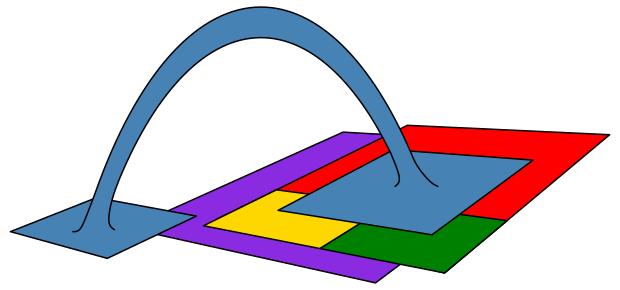
\includegraphics{bridge.png}
  \caption{A depiction of Peirce's Bridge for lines of identity}
  \footnotesize Source:\hspace{3pt}\url{https://commons.wikimedia.org/wiki/File:4CT_Inadequacy_Explanation.svg}
  \labfig{eg-bridge}
\end{marginfigure}

Thus he already identified the problem of readability stemming from having too
many lines or ``cables'' crossing eachother, a well-known concern in the design
of graphical programming languages\todo{Find reference}. This is to be opposed
to critics of the syntax of EG such as Quine, who invented a notation similar to
the lines of identity, and deemed it ``too cumbersome for practical
use''\todo{Find reference}. Also, the other proposed solution of having
so-called \emph{Bridges} is quite interesting, in that it makes the syntax of EG
\emph{three-dimensional}, in order to preserve the continuity of lines. A nice
illustration of the bridge is given in \reffig{eg-bridge}\sidenote{We found this
picture in the Wikipedia article on the \emph{four color theorem}
\cite{noauthor_four_2023}, which is no coincidence: according to Burch
\cite{sep-peirce}, \textit{``Peirce began to research the four-color map
conjecture, to work on the graphical mathematics of de Morgan's associate A. B.
Kempe, and to develop extensive connections between logic, algebra, and
topology, especially topological graph theory. Ultimately these researches bore
fruit in his existential graphs [...]''}. The Wikipedia article on Alfred Kempe
also mentions the following, to be connected with our multiset formalization of
EG \cite{noauthor_alfred_2023}: \textit{``Kempe (1886) revealed a rather marked
philosophical bent, and much influenced Charles Sanders Peirce. Kempe also
discovered what are now called multisets, although this fact was not noted until
long after his death.''}}.

\todo{ Use the following citation to explain how lines of identity are to be
  interpreted as quantifiers, where the term ``endoporeutic'', etymologically
  meaning ``from the outside to the inside'', refers to the relevance of the
  \emph{order} among quantifiers as to their meaning. }
  (\cite{peirce_prolegomena_1906}, p. 531):

\begin{quote}
  In the interpretation of Selectives it is often necessary to observe the rule
which holds throughout the System, that the Interpretation of Existential Graphs
must be \emph{endoporeutic}, that is, the application of a Graph on the Area of
a Cut will depend on the predetermination of the application of that which is on
the Place of the Cut.
\end{quote}
% !TEX root =index.tex
\setchapterpreamble[u]{\margintoc}
\chapter{Flower Calculus}
\labch{flowers}

\epigraph{In a certain flower garden, each flower was either red, yellow, or
blue, and all three colors were represented. A statistician once visited the
garden and made the observation that whatever three flowers you picked, at least
one of them was bound to be red. A second statistician visited the garden and
made the observation that whatever three flowers you picked, at least one was
bound to be yellow. Two logic students heard about this and got into an
argument. The first student said: "It therefore follows that whatever three
flowers you pick, at least one is bound to be blue, doesn't it?" The second
student said: "Of course not!". Which student was right, and why?
}{\textbf{Raymond Smullyan}, \textit{The Flower Garden}, 1985}


\begin{scope}\knowledgeimport{flower}


We introduce the \emph{\kl{flower calculus}}, a novel \kl{proof system} for
\kl{intuitionistic} \kl{predicate logic} based on syntactic objects called
\emph{flowers}. We start by explaining how flowers stem from considerations in
graphical logic, and more specifically from an \kl{intuitionistic} variant of
the \kl{existential graphs} of C. S. Peirce proposed by A. Oostra. Then we
present our inductive syntax for flowers, reminiscent at the same time of the
\kl{nested sequents} of \kl{deep inference} \kl{proof theory}, and the
geometric/\kl{coherent formulas} of categorical logic.

A salient feature of our calculus inherited from \kl{EGs}, is that it is
\emph{fully \kl{iconic}}: it dispenses completely with the traditional notion of
\kl{symbolic} formula, operating instead as a \kl{rewriting system} on flowers
containing only atomic predicates. We also propose a notion of proof geared
towards \kl{analyticity} results à la Gentzen, suggesting new rules absent from
other works on \kl{intuitionistic} \kl{EGs}. This allows us to prove
admissibility theorems for many rules, including Peirce's deletion rule which is
a variant of Gentzen's cut rule. These results are obtained as a consequence of
our soundness and completeness proofs with respect to Kripke semantics, in the
spirit of the \emph{normalization-by-evaluation} technique.

Furthermore, the kernel of rules targetted by completeness is fully
\kl{invertible}, a desirable property in both automated and interactive proof
search. This is illustrated by our implementation of the \kl{Flower\,\,Prover},
an early prototype of \kl{GUI} for \kl{ITPs} that uses the rules of the \kl{flower
calculus} both for \kl{direct manipulation} of flowers in its frontend, and
automated simplification of \kl{goal}s in its backend.

The chapter is organized as follows: in \refsec{IEGs}, we retrace the origin of
Oostra's syntax for \intro{intuitionistic existential graphs} (\reintro{IEGs})
as a natural generalization of the \emph{\kl{scroll}}, an \kl{icon} for
implication introduced by Peirce that inspired the very creation of \kl{EGs}. In
\refsec{Flowers}, we explain how flowers are really just a fun and
\kl{metaphorical} way to draw \kl{IEGs}, and proceed to give them an inductive,
multiset-based syntax as in \refsec{multisets}. In \refsec{Calculus}, we
introduce the full set of \kl{inference rules} of the \kl{flower calculus} as
well as our notion of proof, and prove a few syntactic properties, including two
deduction theorems. In \refsec{Semantics}, we give a direct Kripke semantics to
flowers, avoiding the need for translations to and from formulas. In
\refsec{Soundness}, we show that the rules of the \kl{flower calculus} are \kl{valid}
with respect to our Kripke semantics, and in \refsec{Completeness} we identify a
complete fragment of the system where all rules are both \emph{\kl{analytic}}
and \emph{\kl{invertible}}. This entails the admissibility of all rules outside
of this fragment, and as a consequence the \kl{analyticity} of the system. We
exploit these properties in \refsec{flowers-search} by describing an algorithm
for fully automated proof search in the propositional fragment; unfortunately,
the current version of the algorithm is neither terminating nor complete. Then
in \refsec{flowers-prover} we give an overview of the \kl{Flower\,\,Prover}, a
prototype of \kl{GUI} in the \kl{Proof-by-Action} paradigm whose actions map
directly to the rules of the \kl{flower calculus}, and which integrates nicely
with (a restricted version of) our search procedure. We conclude in
\refsec{Conclusion} by a comparison with some related works, and a discussion of
future works and applications that we envision.


\section{Intuitionistic existential graphs}\labsec{IEGs}

\subsection{The scroll}

In \refsec{alpha}, we presented the syntax of \kl{existential graphs} (\kl{EGs}) as
stemming from two fundamental \kl{icons}: the \kl{sheet of assertion} ($\SA$),
with its ability to represent the conjunction of assertions through
\emph{\kl{juxtaposition}}, and \emph{\kl(eg){cuts}} in $\SA$ that signify the denial or
negation of assertions. However as noted in \refremark{eg-entitative}, the first
interpretation of \kl{juxtaposition} proposed by Peirce was that of
\emph{disjunction}, in his system of \kl{entitative graphs}. According to him,
the \kl{illative transformations} of \kl{EGs} are a necessary consequence of the
\emph{conjunctive} interpretation of \kl{juxtaposition}, as witnessed by the
following excerpt \sidecite[][p.~533]{peirce_prolegomena_1906}:

\begin{quote}
If you carefully examine the above conventions, you will find that they are
simply the development, and excepting in their insignificant details, the
inevitable result of the development of the one convention that if any Graph, A,
asserts one state of things to be real and if another graph, B, asserts the same
of another state of things, then AB, which results from setting both A and B
upon the sheet, shall assert that both states of things are real.
\end{quote}

He goes on to notice:

\begin{quote}
   This was not the case with my first system of Graphs, described in Vol. VII
of The Monist, which I now call Entitative Graphs. But I was forced to this
principle by a series of considerations which ultimately arrayed themselves into
an exact logical deduction of all the features of Existential Graphs.
\end{quote}

Thus the conjunctive reading of \kl{juxtaposition} itself stemmed from ``a
series of considerations'' that ``forced'' Peirce to adopt it. While in this
article he does not give the full ``exact logical deduction of all the features
of Existential Graphs'', he exposes in some details the initial and determining
insight that kickstarted the whole development: the discovery of the \kl{icon}
called the \intro{scroll}. Again, I will let Peirce speak for himself
\cite[pp.~533--534]{peirce_prolegomena_1906}:

\begin{marginfigure}
  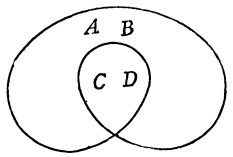
\includegraphics{scroll.png}
  \caption{Peirce's \kl{scroll}}
  \labfig{scroll}
\end{marginfigure}

\begin{quote}
  Accordingly, since logic has primarily in view argument, and since the
conclusiveness of an argument can never be weakened by adding to the premisses
or by subtracting from the conclusion, I thought I ought to take the general
form of argument as the basal form of composition of signs in my
diagrammatization; and this necessarily took the form of a ``scroll'', that is
[...] a curved line without contrary flexure and returning into itself after
once crossing itself, and thus forming an outer and an inner ``close''.
\end{quote}

\reffig{scroll} shows Peirce's drawing of the \kl{scroll} as it appears in
\cite[Fig.~5]{peirce_prolegomena_1906}. He defines its intended meaning like so
\cite[p.~534--535]{peirce_prolegomena_1906}:

\begin{quote}
  I shall call the outer boundary the Wall; and the inner, the Fence. In the
outer I scribed the Antecedent, in the inner the Consequent, of a Conditional
Proposition de inesse. [...][Thus the meaning of \reffig{scroll} is] that if
both A and B are true, then both C and D are true. [...] a Conditional de inesse
(unlike other conditionals) only asserts that either the antecedent is false or
the consequent is true. 
\end{quote}

This shows the \kl{classical} view of Peirce on \kl{EGs}, who interprets the
\kl{scroll} as signifying the \textit{conditional de inesse} --- also called
nowadays \emph{material implication}, and defined here in its disjunctive form,
expressed \kl{symbolically} by $A \limp B \defeq \neg A \lor B$. This is no
coincidence that Peirce based his most fundamental \kl{icon} on implication:
according to Lewis \sidecite[][p.~79]{Lewis1920-LEWASO-4}, he was the one who
introduced the ``illative relation'' of implication into \kl{symbolic} logic in
the first place, by giving it a distinguished \kl{symbol}, and studying
extensively the algebraic laws that govern it (including Peirce's law).

\begin{marginfigure}
  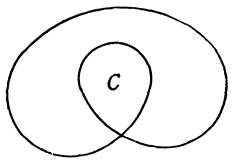
\includegraphics{empty-antecedant.png}
  \caption{Peirce's \kl{scroll} with a blank antecedant}
  \labfig{empty-antecedant}
\end{marginfigure}

\begin{marginfigure}
  $$
  \!\!\!\!\!\!\!\!\stkfig{1}{scroll-empty-antecedant}
  \!\!\!\!\xinvstep{\intro{BA}}~~~~
  G
  $$
  \caption{The rule of \kl{Blank~Antecedant}}
  \labfig{rule-empty-antecedant}
\end{marginfigure}

\subsection{Seeds of intuitionism}

\paragraph{Blank Antecedant}

A first principle that Peirce derives from the \kl{scroll} is the following
\cite[p.~534]{peirce_prolegomena_1906}:

\begin{quote}
  [...] any insertion [is] permitted in the outer close, and any omission from
the inner close. By applying the former clause of this rule to
[\reffig{empty-antecedant}], we see that this \kl{scroll} with the outer close void,
justifies the assertion that if no matter what be true, C is in any case true;
so that the two walls of the \kl{scroll}, when nothing is between them, fall
together, collapse, disappear, and leave only the contents of the inner close
standing, asserted, in the open field.
\end{quote}

\begin{marginfigure}
  ~~~\stkfig{0.8}{scroll-curried}
  \caption{Currying as \kl{scroll} nesting}
  \labfig{scroll-curried}
\end{marginfigure}

\begin{marginfigure}
  \setlength{\fboxsep}{2pt}
\setlength{\arraycolsep}{0pt}
\newcommand{\vsp}{\vspace{-0.5em}}
\newcommand{\stkf}{\tikzfig{0.9}{0.5}}
$$
\begin{array}{r@{\quad}c@{\vsp}}
                                  &\stkf{eg-currying-3} \\
       \xstep{\kl{BA}} &\stkf{eg-uncurrying-1} \\
       \xstep{\kl{Ins}} &\stkf{eg-uncurrying-2} \\
       \xstep{\kl{Deit}} &\stkf{eg-currying-0}
\end{array}
$$
  \caption{\kl{Intuitionistic} proof of currying}
  \labfig{eg-currying}
\end{marginfigure}

\begin{marginfigure}
  \setlength{\fboxsep}{2pt}
\setlength{\arraycolsep}{0pt}
\newcommand{\vsp}{\vspace{-0.5em}}
\newcommand{\stkf}{\tikzfig{0.9}{0.5}}
$$
\begin{array}{r@{\quad}c@{\vsp}}
                                  &\stkf{eg-currying-0} \\
       \xstep{\mathsf{Ins}} &\stkf{eg-currying-1} \\
       \xstep{\mathsf{Deit}} &\stkf{eg-currying-2} \\
       \xstep{\mathsf{BA}} &\stkf{eg-currying-3}
\end{array}
$$

  \caption{\kl{Intuitionistic} proof of uncurrying}
  \labfig{eg-uncurrying}
\end{marginfigure}

This first form of ``collapsing of walls'' is called the rule of \intro{Blank~Antecedant} in \cite{minghui_graphical_2019}, and corresponds \kl{symbolically} to
the equivalence $\top \limp A \semequiv{} A$. The reader might be tempted to see
the ``former clause'' that permits any insertion in the outer close as a special
case of the \kl{Insertion} principle of \kl{Alpha} (\refsec{alpha}). However, we
stress again that Peirce first identified this clause as a feature of the
\kl{scroll}, seen as the \kl{diagrammatic} embodiment of the ``general form of argument''
mentioned in a previous excerpt. The principle of \kl{Insertion} only followed as a
subsequent generalization, stemming from the analysis of the \kl{scroll} into two
nested \kl(eg){cuts} \cite[p.~535]{peirce_prolegomena_1906}:

\begin{quote}
  [...] and you will further see that a scroll is really nothing but one oval
within another.
\end{quote}

To emphasize this point, we will from now on depict \kl{scrolls} as two nested \kl(eg){cuts}
joined at a single point highlighted in orange, as illustrated in
\reffig{rule-empty-antecedant}.

\begin{remark}
  It is interesting to note that the rule of \kl{Blank~Antecedant} is not seen as
  primitive by Peirce, but as a consequence of a \emph{dynamic potential} of the
  \kl{scroll}: namely, the ability to insert anything in the outer close, at will.
  This is another manifestation of Peirce's concern for the question of
  \emph{\kl{illative atomicity}}, and is to be related to the elimination of the
  \kl{Double{-}cut} rule discussed in \refsec{atomicity}.
\end{remark}

\paragraph{Currying}

Peirce was aware of the phenomenon of \emph{currying}, expressed \kl{symbolically} by
the equivalence $A \limp B \limp C \semequiv{} A \land B \limp C$, as witnessed by
the following passage \cite[p.~535]{peirce_prolegomena_1906}:
\begin{quote}
Now, Reader, if you will just take pencil and paper and scribe the scroll
expressing that if $A$ be true, then it is true that if $B$ be true $C$ and $D$
are true [\reffig{scroll-curried}], and compare this with [\reffig{scroll}],
which amounts to the same thing in meaning, you will see that scroll walls with
a void between them collapse even when they belong to different scrolls.
\end{quote}
It is remarkable that he comes to this conclusion by a topological argument,
noting that this second form of ``collapsing of walls'', now involving two
different \kl{scrolls}, follows from the \kl{scroll} beeing composed of two nested
\kl(eg){cuts}. If we reject this interpretation by requiring that the Fence (the
inner oval) stays glued to the Wall (the outer oval), then one cannot derive
currying through the rule of \kl{Double{-}cut}, precisely because the system
only permits to collapse a Wall and a Fence continuously joined in the same
\kl{scroll}, by the weaker rule of \kl{Blank~Antecedant}. Fear not however, as one can
still derive the currying and uncurrying laws in this \kl{intuitionistic} setting,
but through the additional use of the insertion and deiteration rules, as
depicted in \reffig{eg-currying} and \reffig{eg-uncurrying}. Yet we find that
Peirce's insight on the topological explanation of currying in the \kl{classical}
setting remains noteworthy.

\begin{remark}
Note that in \reffig{eg-currying} and \reffig{eg-uncurrying}, we give
\emph{\kl{forward}} proofs that rewrite the premiss of the argument into its
conclusion, rather than \emph{\kl{backward}} proofs that rewrite a \kl{goal}
into the empty $\SA$, as we usually did in previous chapters. \kl{Forward}
proofs correspond to Peirce's usage of the \kl{illative transformations} --- and
thus to what can be found in most of the literature on \kl{EGs}, and have the
advantage of being more economical in space by leaving the \kl{goal} implicit.
One can easily go from a \kl{forward} proof to a \kl{backward} one as shown by
the \emph{deduction theorem} of Sowa \cite[Section 6]{sowa_peirces_2011}, which
also applies in the \kl{intuitionistic} setting by substituting the rule of
\kl{Double{-}cut} with the rule of \kl{Blank~Antecedant}.
\end{remark}

\subsection{Parallel conclusions}

\paragraph{The $n$-ary scroll}

In \cite{oostra_graficos_2010}, A. Oostra proposes to take the above remark
seriously, by reifying the \kl{scroll} as a primitive \kl{icon} of \kl{EGs}
(``\emph{rizo}'' in Spanish), that exists alongside the \kl(eg){cut}
(``\emph{corte}''), and is distinguished from it. In fact he goes further than
this, and proposes to generalize both the \kl(eg){cut} and the \kl{scroll} into
an $n$-ary construction called the \intro{curl} (``\emph{bucle}''), where $n$ is
the number of inner closes, called \emph{loops} (``\emph{lazos}'').
\reffig{five-loops} shows an example of \kl{curl} with five loops. In
\cite{minghui_graphical_2019}, the \kl{curl} is simply called \intro{$n$-ary
scroll}, and is analyzed into the outer area (that enclosed by the Wall) called
the \intro{outloop}, and the inner areas (those enclosed by the $n$ Fences, i.e.
the loops of Oostra) called the \intro{inloops}. Then \kl(eg){cuts} and
\kl{scrolls} are indeed special cases of \kl{$n$-ary scrolls}, respectively with
$n = 0$ and $n = 1$.

\begin{marginfigure}
  \stkfig{1}{five-loops}
  \caption{A \kl{curl} with five loops}
  \labfig{five-loops}
\end{marginfigure}

Like the unary \kl{scroll}, the \kl{$n$-ary scroll} is to be read as an
implication whose antecedant is the content of the \kl{outloop}, and consequent the
content of the \kl{inloops}. The generalization then consists in taking the
\emph{disjunction} of the contents of all \kl{inloops}: this reflects nicely the
etymological meaning of the word ``disjunction'', since the \kl{inloops} enclose
\emph{disjoint} areas of the \kl{outloop} to which they are attached. Then the
\kl[$n$-ary scroll]{$5$-ary scroll} of \reffig{five-loops} is read as the
formula $a \limp b \lor c \lor d \lor e \lor f$; and the \kl[$n$-ary
scroll]{$0$-ary scroll} obtained by removing all \kl{inloops} from the latter as $a
\limp \bot$, since a $0$-ary disjunction is naturally evaluated to its neutral
element $\bot$. This coincides with the \kl{intuitionistic} reading of negation
$\neg A \defeq A \limp \bot$, and is thus consistent with the interpretation of
\kl(eg){cuts} as negations.

\paragraph{Continuity}

\begin{marginfigure}
  $$
\begin{array}{c}
  \begin{array}{cc}
    \stkfig{1}{scroll-disj} & A \lor B \\
    \stkfig{1}{scroll-imp} & A \limp B \\[1em]
    \multicolumn{2}{c}{\not=} \\
    \stkfig{1}{eg-disj} & \neg (\neg A \land \neg B) \\
    \stkfig{1}{eg-imp} & \neg (A \land \neg B)
  \end{array}
\end{array}
$$
  \caption{Continuity, disjunction and implication in \kl{IEGs}}
  \labfig{eg-disj-imp}
\end{marginfigure}

With this interpretation of the \kl{$n$-ary scroll}, the \kl{Alpha} encodings of
disjunction and implication as nested \kl(eg){cuts} are no longer valid, because
they are not \kl{intuitionistically} equivalent to the associated binary and
unary \kl[$n$-ary scroll]{scrolls}. This is illustrated in \reffig{eg-disj-imp},
where the closeness in meaning is reflected \kl{iconically} (but not
\kl{symbolically}) in the fact that the graphs only differ in the
\emph{continuity} (or lack thereof) between \kl{inloops} and their \kl{outloop}. Indeed,
contrary to nested \kl(eg){cuts}, any \kl{$n$-ary scroll} can be drawn by a
\emph{continuous} movement of the pen, producing a self-intersecting curve as
described by Peirce in \cite{peirce_prolegomena_1906}.

This might be related to other manifestations of the notion of continuity in the
semantics of \kl{intuitionistic} logic, such as the well-known Stone-Tarski
interpretation of formulas as topological spaces \cite{stone_topological_1938},
and the interpretation of proofs as continuous maps in the \emph{denotational
semantics} of Dana Scott \sidecite{10.5555/218742.218744}. Before the advent of
Oostra's \kl{IEGs}, Zalamea gave a detailed analysis of Peirce's philosophy of
the \emph{continuum}, how it relates to modern developments in mathematics, and
how it is embodied in \kl{existential graphs} \cite{zalamea_peirces_2003}.
Actually according to Oostra \sidecite[][p.~162]{oostra_advances_2022}, ``the
possibility of developing \kl{intuitionistic} existential graphs was first
suggested by Zalamea in the 1990s \cite{zalamea_ieg_1,zalamea_ieg_2}''.

\subsection{Quantifiers}

More generally, a \kl{$n$-ary scroll} with atoms $G \deq a_1, \ldots, a_m$ in its
\kl{outloop} and $\Delta \deq \begin{pmatrix} a_{1,1} & \ldots & a_{1,p_1} \\
  \vdots & \ddots & \vdots \\
  a_{n,1} & \ldots & a_{1,p_n}
\end{pmatrix}$
in its \kl{inloops}, where each row $H_j$ in $\Delta$ encodes an \kl{inloop}, can be
interpreted as the formula
$$\bigwedge_{i = 1}^{m}{a_i} \limp \bigvee_{j = 1}^{n}\bigwedge_{k = 1}^{p_n}{a_{j,k}}$$
\begin{marginfigure}
  $$
  \!\!\!\!
  \!\!\!\!
  \!\!\!\!
  \begin{array}{c}
    \tikzfig{0.85}{0.85}{curl-geom} \vspace{1.5em}\\
    \forall \bx. \left(\bigwedge G \limp \bigvee_{j = 1}^{n}\exists \bx_j. \bigwedge H_j\right)
  \end{array}
  $$
  \caption{Formula interpretation of the \kl{$n$-ary scroll}}
  \labfig{curl-geom}
\end{marginfigure}
If one adds \emph{\kl(eg){binders}} to the mix (see \refsec{gardens}) by having $\gamma \deq
\garden{\bx}{G}$ as \kl{outloop}, and
$\Xi \deq \begin{pmatrix}
  \bx_1 \\
  \vdots \\
  \bx_n
\end{pmatrix} \cdot \Delta$ as \kl{inloops}, then the interpretation is extended into
the formula
$$\forall \bx. \left(\bigwedge_{i = 1}^{m}{a_i} \limp \bigvee_{j = 1}^{n}\exists \bx_j. \bigwedge_{k = 1}^{p_n}{a_{j,k}}\right)$$
as depicted in \reffig{curl-geom}. Typically, the particular case where $\gamma
\deq \garden{x}{\emptyset}$ and $\Xi \deq (\emptyset) \cdot (p(x))$ encodes the graph
$$\stkfig{1}{scroll-forall}$$
expressing the universal quantification $\forall x. p(x)$, and the case where
$\gamma \deq \garden{\emptyset}{\emptyset}$ and $\Xi \deq (x) \cdot (p(x))$ the graph
$$\stkfig{1}{scroll-exists}$$
expressing the existential quantification $\exists x. p(x)$. The interpretation
is invariant under \kl(eg){polarity}, meaning that for instance the graphs
$$\stkfig{1}{scroll-neg-forall} \text{   and   } \stkfig{1}{scroll-neg-exists}$$
obtained by enclosing the previous graphs in a \kl(eg){cut} are interpreted with the
same quantifiers, as the formulas $\neg \forall x. p(x)$ and $\neg \exists x.
p(x)$. In \kl{Beta}, we would have exploited the \kl{classical} equivalences
$\neg \forall x. A \semequiv{} \exists x. \neg A$ and $\neg \exists x. A \semequiv{}
\forall x. \neg A$ (justified by the \kl{Double{-}cut} principle) in order to
interpret them as $\exists x. \neg p(x)$ and $\forall x. \neg p(x)$, emphasizing
the idea that \kl(eg){positive} and \kl(eg){negative} \kl(eg){binders} encode
respectively $\exists$ and $\forall$. But this is not possible anymore with the
\kl{intuitionistic} interpretation of \kl{$n$-ary scrolls}, where the
$\exists/\forall$ duality is replaced by the \kl{inloop}/\kl{outloop} distinction. In
fact, we are tempted to further qualify this distinction of \emph{adjunction},
following a classical result of Lawvere in the context of categorical logic
\sidecite{lawvere_quantifiers_sheaves}.

\subsection{Coherent formulas}

Lawvere is also known for some contributions to the study of \intro{geometric
logic} \sidecite{lawvere_geometric}, a subset of the formulas of \kl{FOL} first
discovered by Skolem \sidecite{skolem_geometric} that is capable of expressing
many mathematical theories, and has close connections to \emph{topos theory}.
Quite remarkably, the interpretation of \kl{$n$-ary scrolls} coincides exactly
with the class of \intro{coherent formulas}, which are the formulas of
\kl{geometric logic} where infinitary disjunctions are restricted to finitary
ones. There is a difference however: the full syntax of \kl{IEGs} allows for
arbitrary \emph{nestings} of \kl{$n$-ary scrolls} inside eachother, i.e. the
multisets $G$ and $H_j$ in \reffig{curl-geom} can contain \kl{$n$-ary scrolls}
in addition to atoms; while \kl{coherent formulas} are restricted to atoms.

\kl{Coherent formulas} have some nice properties, which might also apply to \kl{IEGs} to
some extent. We only mention two important ones:
\begin{description}
  \item[Completeness] Every \kl{first-order} \kl{theory} has a coherent conservative
  extension, making \kl{coherent formulas} (and thus non-nested \kl{$n$-ary scrolls}) in
  principle as expressive as arbitrary \kl{first-order} formulas
  \sidecite{negri_geometric}.
  
  \item[Automation] \kl{Coherent formulas} benefit from faster proof-search
  procedures compared to arbitrary formulas, making automation more tractable
  computationally. They also allow the direct encoding of many reasoning
  problems, thanks to their use of the full set of connectives and quantifiers
  of \kl{FOL}; and avoiding complex encodings (as can be found e.g. in SMT
  solvers) is crucial in \emph{interactive} theorem proving, where the user and
  the computer manipulate the same formulas in \kl{goal}s
  \sidecite{bezem_automating_2005}. This has been exploited already in some
  domain-specific theorem provers, like the \intro{Larus} prover that
  automatically generates illustrated proofs in geometry\sidenote{Incidentally,
  projective geometry was one of the motivating applications that led Skolem to
  identify the class of \kl{coherent formulas} \cite{bezem_automating_2005}.}
  \sidecite{narboux_larus}.
  
  \begin{remark}
  Thus with \kl{IEGs}, one becomes able to reason \emph{geometrically} on geometric
  formulas that speak about geometry: another beautiful incarnation of the
  reflexivity at work in Peirce's \kl{iconic} logic.
  \end{remark}
\end{description}

\section{Flowers}\labsec{Flowers}

\subsection{Blooming}

As we have seen, the ($n$-ary) \kl[$n$-ary scroll]{scroll} is a powerful
\kl{icon}, because it captures the distinction between \kl{classical} and
\kl{intuitionistic} logic as being a matter of \emph{continuity} between the
space of inputs/hypotheses (\kl{outloop}) and the spaces of outputs/conclusions
(\kl{inloops}), reflecting an intuition discovered much later in the denotational
semantics of the \kl{$\lambda$-calculus}. However as a \kl{diagrammatic}
component to be operated upon through \kl{direct manipulation}, it has one
notable flaw, also shared with the \kl{classical} \kl(eg){cut}-based syntax: it
quickly induces heavy nestings of curves in the plane, making even a simple
graph like that of \reffig{scroll-curried} hard to read for an untrained eye.

\begin{marginfigure}
  $$
  \tikzfig{1}{0.4}{scroll-inside-out}
  $$
  \caption{Turning a \kl[$n$-ary scroll]{$5$-ary scroll} inside-out}
  \labfig{scroll-inside-out}
\end{marginfigure}

Before devising an alternative syntax, one should ask: what are the essential
features of the \kl[$n$-ary scroll]{scroll} that we want to preserve? Following
the previous observations, we identified two of them:
\begin{description}
  \item[Continuity] the \kl[$n$-ary scroll]{scroll is} a self-intersecting
  continuous curve, which can be drawn in one stroke of the pen;
  \item[Polarity] this curve delineates two kinds of areas: \kl{inloops} that have
  the same \kl(eg){polarity} as the area on which the \kl[$n$-ary
  scroll]{scroll} is scribed, and the \kl{outloop} which has the opposite
  \kl(eg){polarity}.
\end{description}

Fortunately, these two properties are preserved when turning \kl{inloops}
\emph{inside-out}, as illustrated in \reffig{scroll-inside-out}. This might be
because the very process of turning inside-out can be seen as a continuous
movement in three-dimensional space, where the \kl{inloops} are rotated around their
intersection points with the \kl{outloop}. In this way, we have effectively divided
the amount of curve-nesting in \kl[$n$-ary scroll]{scrolls} by two. And as an
added bonus, the new \kl{icon} is reminiscent of a \emph{flower}, as if it had
bloomed from its curled bud; or as if the pistol cylinder from
\reffig{five-loops} had transformed into a \emph{pistil}, and its bullet
chambers into \emph{petals}\sidenote{As the saying goes: make love, not war.}.

\begin{marginfigure}
  $$
  \!\!\!\!
  \!\!\!\!
  \!\!\!\!
  \!\!\!\!
  \stkfig{0.65}{flowers}
  $$
  \vspace{-3em}
  \caption{Nested flowers}
  \labfig{flowers}
\end{marginfigure}

From that point onwards, we decided to fully embrace the flower \kl{metaphor}:
first in our drawing style as witnessed in \reffig{flowers}, but also in our
syntactic terminology, to be introduced in the next pages. \kl(eg){Negative}
\kl{outloops} are now drawn as \emph{yellow} pistils for a more colorful experience,
and \kl{inloops} as transparent petals, i.e. of the same color as the area on which
they are scribed. We also drop the requirement that petals should intersect
their pistil at a single point, for purely aesthetic reasons.

\subsection{Multisets}

As we did for \kl{classical} \kl{EGs} in \refsec{multisets} and \refsec{gardens}, we are
now going to distill the syntactic essence of flowers into an inductive,
(multi)set-based data structure. This will allow for a more compact textual
notation, that is better suited to \kl{proof-theoretical} study.

In \refsec{beta}, we explained how the graphs of \kl{Beta} allow to represent
purely relational statements, without function symbols. Since functions are just
deterministic relations, one can in principle formalize any \kl{first-order}
\kl{theory} in this syntax\sidenote{Conversely, every relation can be faithfully
encoded as its characteristic function, which is the basis for the formalization
of mathematics in \emph{\kl{type theories}}.}. However it is much more
convenient to have a dedicated syntax for functions, and we will thus introduce
them as is usually done in predicate calculus.

\begin{definition}[First-order signature]
  A \intro{first-order signature} is a triplet $\mathcal{\Sigma} = (
  \intro*\fsymbs, \intro*\psymbs, \intro*\arity )$, where $\fsymbs$ and $\psymbs$ are
  respectively the countable sets of \emph{function} and \emph{predicate}
  symbols of $\Sigma$, and $\arity : \fsymbs \cup \psymbs \to \nats$ gives an
  \emph{arity} to each symbol.
\end{definition}

\AP
In the following, we assume given a denumerable set of variables $\intro*\vars$
and a \kl{first-order signature} $\Sigma$.

\begin{definition}[Terms]
  The set of terms $\intro*\terms$ is defined inductively as follows:
  \begin{description}
    \item[(Variable)] If $x \in \vars$ then $x \in \terms$;
    \item[(Application)] If $f \in \fsymbs$ and $\tvec{t}
    \in \terms^{\arity(f)}$, then $f(\tvec{t}) \in \terms$.
  \end{description}
\end{definition}

\begin{digression}
  According to the Merriam-Webster dictionary \cite{corolla}, the word
  ``corollary'' has \emph{botanical} etymological roots:
  \begin{quote}
    [...] the seed of corollary was planted initially by the Latin noun corōlla
    meaning ``small wreath of flowers'', which later bloomed into another Latin
    noun, corōllārium, referring to a garland given as a reward as well as to a
    gratuity or an unsolicited payment. [...] The formality of corollary is
    thanks to its formal roots [...]
  \end{quote}
  Then our flower metaphor is a meaningful tribute to these origins: the
  \kl{petals} (\kl{corolla}) of a flower can literally be seen as the
  \emph{corollaries} of its \kl{pistil}, when the latter happens to be true.
\end{digression}

\begin{definition}[Flowers]\labdef{flowers}
  The sets of \emph{flowers} $\intro*\flowers$ and \emph{gardens}
  $\intro*\gardens$ are defined mutually inductively as follows:
  \begin{description}
    \itemAP[(Atom)] If $p \in \psymbs$ and $\tvec{t} \in
    \terms^{\arity(p)}$, then $p(\tvec{t}) \in \flowers$;
    \itemAP[(Garden)] If $\bx \subset \vars$ is a finite set and $\Phi
    \subset \flowers$ a finite multiset, then $\intro*\garden{\bx}{\Phi} \in
    \gardens$;
    \itemAP[(Flower)] If $\gamma \in \gardens$ and $\Delta \subset \gardens$
    is a finite multiset, then $\intro*\flower{\gamma}{\Delta} \in \flowers$.
  \end{description}
\end{definition}

Any finite set $\bx \subset \vars$ of variables is called a \intro{sprinkler},
finite multiset $\Phi \subset \flowers$ of flowers a \intro{bouquet}, and finite
multiset $\Gamma \subset \gardens$ of gardens a \intro{corolla}. We will often
write gardens as $\garden{x_1, \ldots, x_n}{\phi_1, \ldots, \phi_m}$, where the
$x_i$ are called \intro{binders}; and non-atomic flowers as
$\flower{\gamma}{\delta_1 \sep \ldots \sep \delta_n}$, where $\gamma$ is the
\intro{pistil}, and the $\delta_i$ are called \intro{petals}. We write
$\intro*\fset{i}{n}{E_i}$ to denote a finite (multi)set of size $n$ with
elements $E_i$ indexed by $1 \leq i \leq n$. We also omit writing the empty
(multi)set, accounting for it with blank space as is done in \kl{sequent}
notation or in \kl{EGs}; in particular, $\garden{{}}{{}}$ stands for the empty
garden $\garden{\emptyset}{\emptyset}$, $\flower{\gamma}{{}}$ for the flower
with no \kl{petals} $\flower{\gamma}{\emptyset}$, and
$\flower{\gamma}{\garden{{}}{{}}}$ for the flower with one empty \kl{petal}.

Note that the order of precedence of operators is
$\mathop{,} < \garden{{}}{{}} < \mathop{;} < \mathop{\flower{}{}}$
so that for instance, the string
$$\flower{\garden{x_1, x_2}{\phi_1, \phi_2}}{\garden{y_1}{\psi, (\flower{\gamma}{\Delta})} \sep \garden{y_2}{\Phi}}$$
is parsed as the flower
% $$\left(\flower{\left(\garden{\{x_1, x_2\}}{\{\phi_1,
% \phi_2\}}\right)}{\{\left(\garden{\{y_1\}}{\{\psi,
% \left(\flower{\gamma}{\Delta}\right)\}}\right) \sep
% \left(\garden{\{y_2\}}{\Phi}\right)\}}\right)$$ where constructed finite
% (multi)sets are delimited with $\{\}$, and constructed flowers/gardens are
% delimited with $()$.
\vspace{-6em}
$$\stkfig{1}{parsed-flower}$$
\vspace{-6em}

\begin{margintable}
  \centering
  \begin{tabular}{|c|c|}
    \hline
    \bfseries Kind & \bfseries Letters \\
    \hline
    Variables ($\vars$) & $x, y, z$ \\
    Terms ($\terms$) & $t, u, v$ \\
    Flowers ($\flowers$) & $\phi, \psi, \xi$ \\
    Gardens ($\gardens$) & $\gamma, \delta$ \\
    \kl{Sprinklers} & $\bx, \by, \bz$ \\
    Term vectors & $\tvec{t}, \tvec{u}, \tvec{v}$ \\
    \kl{Substitutions} & $\sigma, \tau$ \\
    \kl{Bouquets} & $\Phi, \Psi, \Xi$ \\
    \kl{Corollas} & $\Gamma, \Delta$ \\
    \kl{Contexts} & $\Phi\hole, \Psi\hole, \Xi\hole$ \\
    \kl{Theories} & $\mathcall{T}, \mathcall{U}$ \\
    \hline
  \end{tabular}
  \caption{Notational conventions for meta-variables}
  \labtab{letters}
\end{margintable}

Also to improve readability, we will most of the time omit the garden dot
`$\cdot$' when the \kl{sprinkler} is empty, writing $\Phi$ instead of
$\garden{{}}{\Phi}$.

\begin{remark}
  In some places the choice of letter for meta-variables will be important to
  disambiguate the kind of syntactic object we denote. \reftab{letters}
  summarizes our chosen notational conventions in this respect.
\end{remark}

As usual, we introduce a \emph{\kl{depth}} measure that will allow us to reason
inductively on the structure of flowers:
\begin{definition}[Depth]
  The \reintro{depth} $\intro*\sdepth{-}$ of a flower or garden is defined mutually
  recursively as follows:
  \begin{align*}
    \sdepth{p(\tvec{t})} &= 0 \\
    \sdepth{\garden{\bx}{\Phi}} &= \max_{\phi \in \Phi}{\sdepth{\phi}} \\
    \sdepth{\flower{\gamma}{\Delta}} &= 1 + \max(\sdepth{\gamma}, \max_{\delta \in \Delta}{\sdepth{\delta}})
  \end{align*}
\end{definition}

\subsection{Substitutions}

We now proceed with routine definitions for handling variables and \kl{substitutions}
of terms in flowers.

\begin{definition}[Free variables]\labdef{fv}
  
  The sets of \intro{free variables} $\intro*\fv(-)$ of a term, flower,
  \kl{bouquet} or garden are defined mutually recursively as follows:
  \begin{align*}
    \fv(x) &= \{x\} &
    \fv(\Phi) &= \bigcup_{\phi \in \Phi}{\fv(\phi)} \\
    \fv(f(\tvec{t})) &= \bigcup_{t \in \tvec{t}}{\fv(t)} &
    \fv(\garden{\bx}{\Phi}) &= \fv(\Phi) \setminus \bx \\
    \fv(p(\tvec{t})) &= \bigcup_{t \in \tvec{t}}{\fv(t)} &
    \fv(\flower{\garden{\bx}{\Phi}}{\Delta}) &= \fv(\garden{\bx}{\Phi}) \cup \bigcup_{\garden{\by}{\Psi} \in \Delta}{\fv(\garden{\bx, \by}{\Psi})}
  \end{align*}
  We say that a term, flower, \kl{bouquet} or garden is \emph{closed} when its set of
  \kl{free variables} is empty.
  % The sets of closed terms, flowers and gardens are denoted respectively by
  % $\closed{\terms}$, $\closed{\flowers}$ and $\closed{\gardens}$.
\end{definition}

\begin{remark}\labremark{flower-scope}
Note that the scope of a \kl{binder} located in a \kl{pistil} extends both to the \kl{pistil}
\emph{and} to all its attached \kl{petals}, whereas for a \kl{binder} located in a \kl{petal}
it is limited to said \kl{petal}. This is reflected in the above definition of \kl{free
variables} for (non-atomic) flowers, and is visually explained by the nesting of
curves in an \kl{$n$-ary scroll}.
\end{remark}

\begin{definition}[Bound variables]
  % The set of \emph{bound variables} $\bv(\Phi\hole)$ of a context $\Phi\hole$ is defined
  % inductively as follows:
  % \begin{align*}
  %   \bv(\Psi, \hole) &= \emptyset \\
  %   \bv(\Psi, (\flower{\garden{\bx}{X}}{\Delta})) &= \bx \cup \bv(X) \\
  %   \bv(\Psi, (\flower{\garden{\bx}{\Phi}}{\garden{\by}{X} \sep \Delta})) &= \bx \cup \by \cup \bv(X)
  % \end{align*}
  The sets of \intro{bound variables} $\intro*\bv(-)$ of a flower, \kl{bouquet}
  or garden are defined mutually recursively as follows:
  \begin{align*}
    \bv(p(\tvec{t})) &= \emptyset &
    \bv(\garden{\bx}{\Phi}) &= \bx \cup \bv(\Phi) \\
    \bv(\Phi) &= \bigcup_{\phi \in \Phi}{\bv(\phi)} &
    \bv(\flower{\gamma}{\Delta}) &= \bv(\gamma) \cup \bigcup_{\delta \in \Delta}{\bv(\delta)}
  \end{align*}
\end{definition}

To avoid reasoning about $\alpha$-equivalence, we adopt in this work the
so-called \emph{Barendregt convention} that all variable \kl{binders} are distinct,
both among themselves and from eventual \kl{free variables}. Formally, we assume that
for any \kl{bouquet} $\Phi$, the two following conditions hold:
\begin{enumerate}
  \item computing $\bv(\Phi)$ as a multiset gives the same result as computing
  it as a set;
  \item $\bv(\Phi) \cap \fv(\Phi) = \emptyset$.
\end{enumerate} 
% To preserve this convention, in this paper we will only consider
% \emph{non-circular} substitutions $\sigma$ where $x \not\in \fv(\sigma(x))$ for
% all $x \in \dom(\sigma)$.

To define \kl{substitutions}, we introduce a general notion of \emph{function
\kl{update}}, which will be useful for the semantic evaluation of flowers in
\refsec{Semantics}.

\begin{definition}[Function update]\labdef{update}
  Let $A, B$ be two sets, $f, g : A \to B$ two functions and $R \subseteq A$
  some subset of their domain. The \intro{update} of $f$ on $R$ with $g$ is the
  function defined by:
  $$
  (f \intro*\upd{R} g)(x) =
  \begin{cases}
    g(x) &\text{if $x \in R$} \\
    f(x) &\text{otherwise}
  \end{cases}
  $$
  $\update{-}{-}{-}$ is left-associative, that is
  $\update{f}{R}{\update{g}{S}{h}} = \update{(\update{f}{R}{g})}{S}{h}$. Also if
  $f$ or $g$ is the identity function $\intro*\idsubst$ we omit writing it, i.e.
  $\update{f}{R}{{}} = \update{f}{R}{\idsubst}$ and $\update{{}}{R}{g} =
  \update{\idsubst}{R}{g}$.
\end{definition}

\begin{definition}[Substitution]
  A \intro{substitution} is a function $\sigma : \vars \to \terms$ with a finite
  \intro{support} $\dom(\sigma) = \compr{x}{\sigma(x) \not= x}$. By abuse of
  notation, we will write $\sigma : \bx \to \terms$ to denote a \kl{substitution}
  $\sigma$ whose \kl{support} is $\bx$. The domain of \kl{substitutions} is extended to
  terms, flowers, \kl{bouquets} and gardens mutually recursively as follows:
  \begin{align*}
    \sigma(f(t_1, \ldots, t_n)) &= f(\sigma(t_1), \ldots, \sigma(t_n)) \\
    \sigma(p(t_1, \ldots, t_n)) &= p(\sigma(t_1), \ldots, \sigma(t_n)) \\
    \sigma(\phi_1, \ldots, \phi_n) &= \sigma(\phi_1), \ldots, \sigma(\phi_n) \\
    \sigma(\garden{\mathbf{x}}{\Phi}) &=
      \garden{\mathbf{x}}{\restr{\sigma}{\mathbf{x}}(\Phi)} \\
    \sigma(\flower{\garden{\mathbf{x}}{\Phi}}{\delta_1 \sep \ldots \sep \delta_n}) &=
      \flower{\sigma(\garden{\mathbf{x}}{\Phi})}{\restr{\sigma}{\mathbf{x}}(\delta_1) \sep \ldots \sep \restr{\sigma}{\mathbf{x}}(\delta_n)}
  \end{align*}

\end{definition}

\begin{definition}[Capture-avoiding substitution]
  We say that a \kl{substitution} $\sigma : \bx \to \terms$ is
  \intro{capture-avoiding} in a \kl{bouquet} $\Phi$ if $\fv(\sigma(x)) \cap \bv(\Phi)
  = \emptyset$ for every $x \in \bx$.
  % $\fv(\sigma(x)) \cap \bv(\phi) = \emptyset$ for every $x \in
  % \bx$, or $\bx \cap \fv(\phi) = \emptyset$.
  % \begin{itemize}
  %   \item $\phi = p(\tvec{t})$;
  %   \item $\phi =
  %   \flower{\garden{\by}{\Phi}}{\fset{i}{n}{\garden{\bz_i}{\Psi_i}}}$,
  %   $\fv(\sigma(x)) \cap \left(\by \cup \bigcup_{i = 1}^{n}{\bz_i}\right) =
  %   \emptyset$ for every $x \in \bx \cap \left(\fv(\Phi) \cup \bigcup_{i =
  %   1}^{n}{\fv(\Psi_i)}\right)$, and $\sigma$ is capture-avoiding in $\Phi \cup
  %   \bigcup_{i = 1}^{n}{\Psi_i}$.
  %   % \item $\bx \cap \fv(\phi) = \emptyset$.
  % \end{itemize}
\end{definition}

\section{Calculus}\labsec{Calculus}

\subsection{Preliminary definitions}

\paragraph{Contexts}

Equipped with an inductive syntax, we can now express formally the \kl{inference
rules} of our \kl{flower calculus}, just as we did for \kl{Alpha}
(\refsec{multisets}) and \kl{Beta} (\refsec{gardens}). There, graphs and their
\kl{contexts} were defined as multisets of \kl(beta){nodes}, which have now turned
into \kl{bouquets} of flowers:

\begin{definition}[Context]
  A \intro{context} $\Phi\hole$ is a \kl{bouquet} which contains exactly one
  occurrence of a special flower written $\hole$, called its \reintro{hole}. The
  \kl{hole} can always be \emph{filled} (substituted) with any other
  \kl{bouquet} $\Psi$ or \kl{context} $\Xi\hole$, producing a new \kl{bouquet}
  $\cfill{\Phi}{\Psi}$ or \kl{context} $\cfill{\Phi}{\Xi\hole}$. In particular,
  filling with the empty \kl{bouquet} will yield a \kl{bouquet}
  $\cfill{\Phi}{\phantom{\Phi}}$, which is just $\Phi\hole$ with its \kl{hole}
  removed. A \emph{flower context} $\phi\hole$ is a \kl{context} with exactly
  one flower.
\end{definition}

\begin{definition}[Depth]
  The \intro{depth} $\intro*\cdepth{\Phi\hole}$ of a \kl{context} $\Phi\hole$ is
  defined recursively as follows:
  \begin{align*}
    \cdepth{\Psi, \hole} &= 0 \\
    \cdepth{\Psi, (\flower{\garden{\bx}{\Phi\hole}}{\Delta})} &= 1 + \cdepth{\Phi\hole} \\
    \cdepth{\Psi, (\flower{\gamma}{\garden{\bx}{\Phi\hole} \sep \Delta})} &= 1 + \cdepth{\Phi\hole}
  \end{align*}
\end{definition}

Contrarily to \kl{EGs} (\refdef{eg-inv}), the number of inversions of a \kl{context} does
not coincide with its \kl{depth}, since \kl{petals} increase \kl{depth} but preserve \kl{polarity}:

\begin{definition}[Inversions]
  The number of \emph{inversions} $\intro*\inv(\Phi\hole)$ of a \kl{context} $\Phi\hole$ is
  defined recursively by:
  \begin{align*}
    \inv(\Psi, \hole) &= 0 \\
    \inv(\Psi, (\flower{\garden{\bx}{\Phi\hole}}{\Delta})) &= \inv(\Phi\hole) + 1 \\
    \inv(\Psi, (\flower{\gamma}{\garden{\bx}{\Phi\hole} \sep \Delta})) &= \inv(\Phi\hole)
  \end{align*}
\end{definition}

\begin{definition}[Polarity]
  \phantomintro{polarity}
  We say that a \kl{context} $\Phi\hole$ is \intro{positive} if
  $\inv(\Phi\hole)$ is even, and \intro{negative} otherwise. We denote \kl{positive}
  and \kl{negative} \kl{contexts} respectively by $\Phi^+\hole$ and $\Phi^-\hole$.
\end{definition}

\paragraph{Pollination}

In order to formulate the equivalent of the (de)iteration rules of \kl{EGs} for
flowers, we introduce a \emph{\kl{pollination}} relation that captures the
availability of a flower in a given \kl{context}, akin to the \emph{justification}
relation of \refsubsec{scientific-way}:

\begin{definition}[Pollination]\labdef{pollination}
  
  We say that a flower $\phi$ can be \intro{pollinated} in a \kl{context}
  $\Phi\hole$, written $\intro*\chyp{\phi}{\Phi\hole}$, when there exists a
  \kl{bouquet} $\Psi$ with $\phi \in \Psi$ and \kl{contexts} $\Xi\hole$ and
  $\Xi_{0}$ such that either:
  \begin{description}
    \itemAP[(\intro{Cross-pollination})] $\Phi\hole = \cfill{\Xi}{\Psi,
    \Xi_{0}}$;
    \itemAP[(\intro{Self-pollination})] $\Phi\hole =
    \cfill{\Xi}{\flower{\garden{\bx}{\Psi}}{\garden{\by}{\Xi_{0}}
    \sep \Delta}}$ for some $\bx, \by, \Delta$.
  \end{description}
  A \kl{bouquet} $\Psi$ can be \kl{pollinated} in $\Phi\hole$, written
  $\chyp{\Phi}{\Phi\hole}$, if $\chyp{\phi}{\Phi\hole}$ for all $\phi \in \Phi$.
\end{definition}

\begin{marginfigure}
  $$
  \!\!\!\!
  \!\!\!\!
  \!\!\!\!
  \begin{array}{c}
    \tikzfig{1}{0.5}{cross-pollination} \vspace{-2em} \\
    \text{\textit{\kl{Cross-pollination}}} \vspace{-1em} \\
    \tikzfig{1}{0.5}{self-pollination} \vspace{-2em} \\
    \text{\textit{\kl{Self-pollination}}}
  \end{array}
  $$
  \caption{\kl{Pollination} in flowers}
  \labfig{pollination}
\end{marginfigure}

We now employ the \kl{metaphor} of \emph{\kl{pollination}} to speak about
(de)iteration in flowers. This is illustrated in \reffig{pollination}, where the
blue dot marks the location of the justifying/\kl{pollinating} occurrence of
$\phi$, and the red dots all the areas that it (locally)
justifies/\kl{pollinates}, and thus where $\phi$ can be
(de)iterated\sidenote{\reffig{pollination} summarizes visually the flow of
information in flowers, just like \reffig{eg-local-justification} summarized the
flow of information in \kl{EGs}, and \reffig{bubbles-porosity} in bubbles. From
a UI point of view, all these figures can be understood as kind of
``cheatsheets'', that indicate with arrows the allowed drag-and-drop moves for
importing a statement (the source of the \kl{DnD}) into a new \kl{context} (the
destination of the \kl{DnD}).}. We distinguish two cases of
\emph{\kl{cross-pollination}} and \emph{\kl{self-pollination}}, as botanists do
when describing the reproduction of flowers. This distinction does not exist in
\kl{classical} \kl{EGs}, because \kl{pistils} and \kl{petals} are both
identified as instances of \kl(eg){cuts}\sidenote{The same phenomenon is at work
in \emph{\kl{subformula linking}} (\refch{sfl}): \kl{self-pollination} and
\kl{cross-pollination} correspond respectively to the \emph{\kl(dnd){backward}}
$\back$ and \emph{\kl(dnd){forward}} $\forw$ \kl{interaction operators}, which
are collapsed into a single interaction operator $\ast$ in the original
formulation of \kl{subformula linking} for classical linear logic
\cite{Chaudhuri2013}.}. If we were to replace \kl{binders} by \kl{LoIs}
(\kl{lines of identity}, see \refsec{beta}), then the \kl{pollination} relation would
also prescribe in which areas \kl{LoIs} can be extended/iterated, providing an
explanation for the scope of \kl{binders} (\refremark{flower-scope}).

\subsection{Rules}

As has become standard in this thesis, we define the \kl{flower calculus} as a
\emph{\kl{rewriting system}} on \kl{bouquets}, presented in \reffig{flower-calculus} as a
set of unary \kl{deep inference} rules: when read \emph{top-down}, they correspond to
usual inferences from premiss to conclusion, and will be justified by the
soundness theorem of \refsec{Soundness}.
But the more interesting direction, and the one around which the calculus has
been designed, is when you read the rules \emph{bottom-up}: then they are indeed
\kl{rewriting rules}, telling you the different ways in which you can choose to
simplify a \kl{goal}. This is how the \emph{graphical} version of the rules is
presented in \reffig{natural-graphical} and \reffig{cultural-graphical}.

Let us now describe the rules in more detail, starting with the fragment that is
a direct adaptation of the rules of \kl{Beta} (\reffig{beta}):

\begin{description}
  \item[Blank~Antecedant (\kl{epis})]
    
    \begin{marginfigure}
      $$
      \R[\intro{epis{\da}}]
        {\Phi}
        {\flower{\garden{{}}{{}}}{\garden{{}}{\Phi}}}
      $$
      \caption{Converse of \kl{epis} rule}
      \labfig{flowers-episda}
    \end{marginfigure}

    It allows to enclose any \kl{bouquet} in a \kl{petal} attached to an \textsf{(e)}mpty
    \textsf{(pis)}til. This is one direction of the rule of \kl{Blank~Antecedant} (\reffig{rule-empty-antecedant}), which is a weaker,
    \kl{intuitionistic} version of the \kl{classical} rule \kl{Dcut{\ua}} of
    \kl{Alpha} and \kl{Beta}. The other direction (rule \kl{epis{\da}} in
    \reffig{flowers-episda}) is actually \kl{admissible}, which might be related
    to the co-admissibility of \kl{Dcut{\da}} in \kl{Alpha} (\refcor{adm-ins}).

  \item[(De)iteration (\kl{poll{\da}}, \kl{poll{\ua}})]
    Renamed \emph{\textsf{(poll)}ination} rules, they correspond to the rules
    \kl{Iter} and \kl{Deit} of \kl{Alpha} and \kl{Beta}, but reformulated with
    the \kl{pollination} relation (\refdef{pollination}). In fact in their
    textual presentation of \reffig{flower-calculus}, they are more general than
    (de)iteration rules, because \refdef{pollination} allows the
    \kl{pollinating} \kl{bouquet} $\Phi$ to be \emph{scattered} in the
    \kl{context} $\Xi\hole$, i.e. its flowers need not be located in the same
    area. On the contrary in the graphical presentation of
    \reffig{natural-graphical}, they are less general since only one flower can
    be \kl{pollinated} at a time, rather than an entire \kl{bouquet} of flowers
    residing in the same area. But it is easy to see that all these variants are
    equivalent in deductive power, since the \kl{pollination} of a \kl{bouquet}
    (however scattered) can always be simulated by the successive
    \kl{pollinations} of each of its flowers.

  \item[Insertion/Deletion (\kl{grow}, \kl{crop}, \kl{pull}, \kl{glue})]
    They correspond to the rules \kl{Ins} and \kl{Del} of \kl{Alpha} and
    \kl{Beta}, but have doubled in number to account for the syntactic
    distinction between \kl{pistils} and \kl{petals}. More precisely, rules \kl{grow} and
    \kl{crop} allow to insert and delete entire flowers, while rules \kl{pull}
    and \kl{glue} deal with \kl{petals}. As for \kl{pollination} rules, manipulating
    single flowers/\kl{petals} (graphical version) or entire \kl{bouquets}/\kl{corollas}
    (textual version) does not change the deductive power of the rules.
    
  \item[Unification (\kl{ipis}, \kl{ipet}, \kl{apis}, \kl{apet})]
    Rules \kl{ipis} and \kl{ipet} allow to \textsf{(i)}nstantiate a
    \kl{sprinkler} located respectively in a \textsf{(pis)}til ($\forall$) and a
    \textsf{(pet)}al ($\exists$) with an arbitrary \kl{substitution}, while
    rules \kl{apis} and \kl{apet} do the opposite operation of
    \textsf{(a)}bstracting a set of terms by introducing a \kl{sprinkler}. They
    correspond respectively to a generalization of the rules \kl{Unif{\ua}} and
    \kl{Unif{\da}} of \kl{Beta}, where the variable \kl{substitution} $\{z/y\}$
    becomes an arbitrary \kl{substitution} $\sigma$. Once again, we have twice
    the amount of rules to account for the \kl{pistil}/\kl{petal} distinction,
    which is not surprising since in the \kl{LoI} syntax of \kl{EGs}, they are
    special cases of \kl{Insertion}/\kl{Deletion}. Note that for the
    instantiation rules \kl{ipis}/\kl{ipet} to be \kl{invertible}, we duplicate
    the whole flower/\kl{petal} where the \kl{sprinkler} occurs, mirroring what
    is done in multi-conclusion \kl{sequent calculi} (see \reffig{multi-inst}).
\end{description}

The last two rules mainly handle the behavior of disjunctive and absurd
statements, i.e. flowers with respectively $n \geq 2$ and $n = 0$ \kl{petals}, and
are closer to sequent-style introduction/\kl{elimination rules}:

\begin{description}
  \item[Disjunction Introduction (\kl{epet})]
    It allows to erase any flower with an \textsf{(e)}mpty \textsf{(pet)}al.
    According to Oostra \cite[p.~109]{oostra_advances_2022}, Peirce already
    identified \kl{epet} as a component of his decision procedure for
    \kl{Alpha} (it is simply called ``Operation 1'' in
    \cite{oostra_advances_2022}). This is no coincidence, since we precisely
    came up with this rule when trying to design a decision procedure for
    flowers (see \refsec{flowers-search}).

  \item[Disjunction/Absurdity Elimination (\kl{srep})]
    It corresponds to a $n$-ary generalization of the \kl{left introduction
    rule} for disjunction in \kl{sequent calculus}, the $0$-ary case capturing
    absurdity elimination (\textit{ex falso quodlibet}). The binary case is also
    used in the \kl{IEGs} system of \cite{minghui_graphical_2019}, together with
    its converse. The name \kl{srep} is short for
    \textsf{(s)}elf-\textsf{(rep)}roduction, which is more clearly visualized in
    the graphical version of the rule in \reffig{natural-graphical}. Through the
    \kl{Curry-Howard correspondence}, it can be related to the \emph{pattern-matching
    generator} found in modern editors of some functional programming languages,
    such as the Hazel structure editor and the \kl{Agda} \kl{proof assistant}
    \sidecite{yuan-live-2023}.
\end{description}

\begin{table}
  \vspace{-1em}
  $$
  \newcommand{\nhsp}{\!}
  \def\arraystretch{1.5}
  \begin{array}{|c|c|c|c|c|c|c|c|c|c|}
    \hline
    \multicolumn{2}{|c|}{\text{\textbf{Connective}}} &
    \top & \land & \bot & \neg & \limp & \lor & \forall & \exists \\
    \hhline{|==|=|=|=|=|=|=|=|=|}
    \multicolumn{2}{|c|}{\text{\textbf{\kl{Corolla}}}} &
    \geq & = & < & < & = & > & = & = \\
    \hline
    % \multicolumn{2}{|c|}{\text{\textbf{Depth}}} &
    % < & < & = & - & - & - & - & - \\
    % \hline
    \multirow{2}{*}{\text{\textbf{\kl{Bouquets}}}}
    % & \text{\small\textbf{Top-level}} &
    % < & > & = & = & = & = & = & = \\
    % \cline{2-10}
    & \text{\small\textbf{\kl{Pistil}}} &
    - & < & < & = & \leq & < & < & < \\
    \cline{2-10}
    & \text{\small\textbf{\kl{Petals}}} &
    < & > & - & - & = & = & = & = \\
    \hline
    \multirow{2}{*}{\text{\textbf{\kl{Sprinklers}}}}
    & \text{\small\textbf{\kl{Pistil}}} &
    - & < & < & < & < & < & \geq & < \\
    \cline{2-10}
    & \text{\small\textbf{\kl{Petals}}} &
    < & < & - & - & < & < & < & \geq \\
    \hline
  \end{array}
  $$
  \caption{Fragments of \kl{intuitionistic} logic as cardinality constraints on flowers}
  \labtab{flowers-fragments}
\end{table}

The rules of the \kl{flower calculus} have an interesting property: they are
mostly \emph{arity-agnostic}, i.e. they work uniformly on flowers, \kl{bouquets}
and gardens with any number of \kl{petals}, flowers and \kl{binders}. In
particular, this means that the same rules can be used to capture provability in
almost any \emph{fragment} of \kl{intuitionistic} \kl{predicate logic},
understood as any subset $\mathfrak{F} \subset \flowers$ of the set of all
flowers\sidenote{The only exception seems to be the rule (\kl{ipis}) (resp.
\kl{ipet}), whose duplication of flowers (resp. \kl{petals}) prevents $\forall$
(resp. $\exists$) from being provable without $\land$ (resp. $\lor$). This can
be fixed by simply removing the duplication, and polarizing the \kl{context} of
application as for the rule \kl{apis} (resp. \kl{apet}), at the cost of making
the rule non-\kl{invertible}.}. \reftab{flowers-fragments} shows how all the
usual \kl{symbolic} connectives can be expressed by \emph{cardinality}
constraints on set-based syntactic constructs: $<$, $\leq$, $=$, $\geq$, $>$
correspond respectively to a cardinality smaller, smaller or equal, equal,
greater or equal, and greater than $1$; and `$-$' denotes the absence of
constraint. These constraints are then taken \emph{conjunctively} for a single
connective (column-wise); and they can be freely mixed \emph{disjunctively}
(row-wise), in order to capture any fragment corresponding to a subset of
connectives.

\begin{figure*}[h!]
  \begin{framed}
{\textsc{Nature} $\intro*\Nature$}
\vspace{1.5em}
\begin{mathpar}
  \R[\intro{poll{\da}}]
    {\cfill{\Xi}{\phantom{\Phi}}}
    {\cfill{\Xi}{\Phi}}
  \and
  \R[\intro{poll{\ua}}]
    {\cfill{\Xi}{\Phi}}
    {\cfill{\Xi}{\phantom{\Phi}}}
  \\
  \R[\intro{epis}]
    {\flower{\garden{{}}{{}}}{\garden{{}}{\Phi}}}
    {\Phi}
  \and
  \R[\intro{epet}]
    {}
    {\flower{\gamma}{\garden{{}}{{}} \sep \Delta}}
  \\
  \R[\intro{ipis}]
    {(\flower{\garden{\bx}{\sigma(\Phi)}}{\sigma(\Delta)}), (\flower{\garden{\bx, \by}{\Phi}}{\Delta})}
    {\flower{\garden{\bx, \by}{\Phi}}{\Delta}}
  \and
  \R[\intro{ipet}]
    {\flower{\gamma}{\garden{\bx}{\sigma(\Phi)} \sep \garden{\bx, \by}{\Phi} \sep \Delta}}
    {\flower{\gamma}{\garden{\bx, \by}{\Phi} \sep \Delta}}
  \\
  \R[\intro{srep}]
    {\flower{\garden{\bx}{\Phi}}{\garden{{}}{\fset{i}{n}{\flower{\gamma_i}{\Delta}}}}}
    {\flower{\garden{\bx}{\Phi, (\flower{\garden{{}}{{}}}{\fset{i}{n}{\gamma_i}})}}{\Delta}}
\end{mathpar}

\vspace{3em}

{\textsc{Culture} $\intro*\Culture$}
\vspace{1.5em}
\begin{mathpar}
  \R[\intro{grow}]
    {\cfill{\Xi^+}{\Phi}}
    {\cfill{\Xi^+}{\phantom{\Phi}}}
  \and
  \R[\intro{crop}]
    {\cfill{\Xi^-}{\phantom{\Phi}}}
    {\cfill{\Xi^-}{\Phi}}
  \\\\
  \R[\intro{pull}]
    {\cfill{\Xi^+}{\flower{\gamma}{\Delta}}}
    {\cfill{\Xi^+}{\flower{\gamma}{\Gamma \sep \Delta}}}
  \and
  \R[\intro{glue}]
    {\cfill{\Xi^-}{\flower{\gamma}{\Gamma \sep \Delta}}}
    {\cfill{\Xi^-}{\flower{\gamma}{\Delta}}}
  \\\\
  \R[\intro{apis}]
    {\cfill{\Xi^+}{\flower{\garden{\bx, \by}{\Phi}}{\Delta}}}
    {\cfill{\Xi^+}{\flower{\garden{\bx}{\sigma(\Phi)}}{\sigma(\Delta)}}}
  \and
  \R[\intro{apet}]
    {\cfill{\Xi^-}{\flower{\gamma}{\garden{\bx, \by}{\Phi} \sep \Delta}}}
    {\cfill{\Xi^-}{\flower{\gamma}{\garden{\bx}{\sigma(\Phi)} \sep \Delta}}}
\end{mathpar}

\vspace{3em}

In the rules \kl{poll{\da}} and \kl{poll{\ua}}, we assume that
$\chyp{\Phi}{\Xi\hole}$.

In the rules \kl{ipis}, \kl{apis} (resp. \kl{ipet}, \kl{apet}), we
assume some \kl{substitution} $\sigma : \by \to \terms$ that is
capture-avoiding in $\flower{\garden{{}}{\Phi}}{\Delta}$ (resp. $\Phi$).
\end{framed}
  \caption{Rules of the \kl{flower calculus}}
  \labfig{flower-calculus}
\end{figure*}

\subsection{Proofs}

Our notions of derivation and proof are essentially the same as the ones given
for \kl{EGs} in \refsec{multisets}, except that we distinguish from the outset between
two kinds of derivations, stemming from our partitioning of the rules into two
sets: the \intro{natural} rules denoted by $\Nature$, and the \intro{cultural}
rules denoted by $\Culture$. In particular, every $\Nature$-rule is both
\emph{\kl{analytic}} (i.e. every atom in the premiss already appears in the
conclusion) and \emph{\kl{invertible}} (this will be shown in \refsec{Soundness}); on
the contrary, all $\Culture$-rules are \emph{non-\kl{invertible}}, and they will be
shown to be \emph{\kl{admissible}} in \refsec{Completeness}.

\begin{definition}[Derivation]
  Given a set of rules $\mathsf{R}$, we write $\Phi \intro*\step{\mathsf{R}}
  \Psi$ to indicate a rewrite \emph{step} in $\mathsf{R}$, that is an instance
  of some $r \in \mathsf{R}$ from \reffig{flower-calculus} with $\Psi$ as
  premiss and $\Phi$ as conclusion. We just write $\Phi \reintro*\step{} \Psi$
  to mean $\Phi \step{\Nature\cup\Culture} \Psi$. A \emph{derivation} $\Phi
  \nsteps{n}{\mathsf{R}} \Psi$ is a sequence of rewrite steps $\Phi_0
  \step{\mathsf{R}} \Phi_1 \ldots \step{\mathsf{R}} \Phi_n$ with $\Phi_0 =
  \Phi$, $\Phi_n = \Psi$ and $n \geq 0$. Generally the length $n$ of the
  derivation does not matter, and we just write $\Phi
  \reintro*\steps{\mathsf{R}} \Psi$. Finally, natural derivations are closed
  under arbitrary \kl{contexts}: for every \kl{context} $\Xi\hole$, $\Phi
  \step{\Nature} \Psi$ implies $\cfill{\Xi}{\Phi} \step{\Nature}
  \cfill{\Xi}{\Psi}$. We write $\Phi \intro*\lstep{\Nature} \Psi$ to denote a
  \intro{shallow} natural step, i.e. a direct instance of a natural rule in the
  empty \kl{context}.
\end{definition}

\newpage
The following lemma is the \kl{flower calculus} equivalent of \reflemma{eg-posclos}
for \kl{EGs}:

\begin{lemma}[Positive closure]\lablemma{flowers-posclos}
  If $\Phi \step{} \Psi$, then $\Xi^+\select{\Phi} \step{} \Xi^+\select{\Psi}$.
\end{lemma}
\begin{proof}
  In the case of a natural step $\Phi \step{\Nature} \Psi$, this is immediate
  by definition. Otherwise we have a cultural step $\Xi'\select{\Phi_0}
  \step{\Culture} \Xi'\select{\Psi_0}$. Then either $\Xi'\hole$ is \kl{positive},
  and $\inv(\Xi^+\select{\Xi'\hole}) = \inv(\Xi^+\hole) + \inv(\Xi'\hole)$ is
  even since it is the sum of two even numbers; or $\Xi'\hole$ is \kl{negative}, and
  $\inv(\Xi^+\select{\Xi'\hole})$ is odd since it is the sum of an even and an
  odd number. In both cases $\Xi^+\select{\Xi'\hole}$ has the same \kl{polarity} as
  $\Xi'\hole$, and thus the same rule can be applied.
\end{proof}

Now we can define our usual ``\kl{goal}-oriented'' notion of proof:

\begin{definition}[Proof]\labdef{flowers-proof}
  A \emph{proof} of a \kl{bouquet} $\Phi$ is a derivation $\Phi \steps{} \emptyset$.
\end{definition}

In Peircean terms, the empty \kl{bouquet} is the blank $\SA$. Then proving a
\kl{bouquet} amounts to erasing it completely from $\SA$, thus reducing it to
vacuous truth. \reffig{flowers-proof-example} shows an example of
$\Nature$-proof in the \kl{flower calculus}, both in textual and graphical
syntax. Note that we used a non-duplicating version of the rules \kl{ipis} and
\kl{ipet}, in order to save some space in the graphical presentation.

If we want to speak about \emph{relative} truth, i.e. $\Phi$ is true under the
assumption that $\Psi$ is, we can simply rely on the existence of a derivation
$\Phi \steps{} \Psi$ in the full \kl{flower calculus}. This will be justified by
the soundness of all rules (\refthm{flowers-soundness}) as well as a
\emph{strong} completeness result (\refcor{flowers-strong-completeness}), that
relies on the following strong deduction theorem:

\begin{theorem}[Strong deduction]\labthm{flowers-strong-deduction}
  $\Phi \steps{} \Psi$ if and only if $\flower{\Psi}{\Phi} \steps{} \emptyset$.
\end{theorem}
\begin{proof}
  Suppose that $\Phi \steps{} \Psi$. Then we have:
  $$
  \begin{array}{rlll}
    \flower{\Psi}{\Phi}
    &\steps{} &\flower{\Psi}{\Psi} &\text{(Hypothesis + \reflemma{flowers-posclos})}\\
    &\step{\kl{poll{\da}}} &\flower{\Psi}{\cdot} &\\
    &\step{\kl{epet}} &\emptyset &
  \end{array}
  $$
  
  In the other direction, suppose that $\flower{\Psi}{\Phi} \steps{} \emptyset$.
  Then we have:
  $$
  \begin{array}{rlll}
    \Phi
    &\step{\kl{epis}} &\flower{}{\Phi} &\\
    &\step{\kl{grow}} &(\flower{\Psi}{\Phi}),(\flower{}{\Phi}) &\\
    &\step{\kl{poll{\ua}}} &(\flower{\Psi}{\Phi}),(\flower{(\flower{\Psi}{\Phi})}{\Phi}) &\\
    &\steps{} &\flower{(\flower{\Psi}{\Phi})}{\Phi} &\text{(Hypothesis + \reflemma{flowers-posclos})}\\
    &\step{\kl{grow}} &\Psi,(\flower{(\flower{\Psi}{\Phi})}{\Phi}) &\\
    &\step{\kl{poll{\da}}} &\Psi,(\flower{(\flower{}{\Phi})}{\Phi}) &\\
    &\step{\kl{srep}} &\Psi,(\flower{}{(\flower{\Phi}{\Phi})}) &\\
    &\step{\kl{poll{\da}}} &\Psi,(\flower{}{(\flower{\Phi}{\cdot})}) &\\
    &\step{\kl{epet}} &\Psi,(\flower{}{\cdot}) &\\
    &\step{\kl{epet}} &\Psi
  \end{array}
  $$
\end{proof}

Contrary to full derivability, \kl{natural} derivability $\Phi \steps{\Nature}
\Psi$ is too weak to satisfy a strong deduction theorem. This is a consequence
of the fact that $\Nature$-rules are \emph{\kl{invertible}}, and thus can only
relate equivalent \kl{bouquets}. Indeed, as soon as $\flower{\Psi}{\Phi}$
is $\Nature$-provable but the converse $\flower{\Phi}{\Psi}$ is not, it follows
from the completeness of $\Nature$-rules that $\Phi$ and $\Psi$ are not
equivalent: thus $\Phi \notsteps{\Nature} \Psi$, contradicting the strong
deduction statement.

\AP
$\flower{\Psi}{\Phi} \steps{} \emptyset$. In fact this is closer to what one
would find in \kl{sequent calculus}, where hypothetical proofs are closed
derivations of hypothetical sequents, not open derivations. The difference is
that \kl{sequents} capture only the \intro(implication){first-order} implicative
structure of logic\sidenote{As opposed to \intro(implication){higher-order},
i.e. \kl(sfl){negatively} nested implications.}, while flowers capture the full
structure of \kl{intuitionistic} \kl{predicate logic}. This allows for a nice
generalization of the notion of hypothetical provability, which will be useful
in the completeness proof of \refsec{Completeness}. 

\begin{definition}[Hypothetical provability]
  Given two \kl{bouquets} $\Phi, \Psi$, we say that $\Phi$ is
  \emph{hypothetically provable} from $\Psi$ in a fragment $\mathsf{R}$ of
  rules, written $\Psi \intro*\entails{\mathsf{R}} \Phi$, if for every
  \kl{context} $\Xi\hole$ such that $\chyp{\Psi}{\Xi\hole}$, $\cfill{\Xi}{\Phi}
  \step{\mathsf{R}} \cfill{\Xi}{\phantom{\Phi}}$. We write $\Psi
  \reintro*\entails{} \Phi$ to denote hypothetical provability in the full
  \kl{flower calculus}.
\end{definition}

\begin{lemma}[Reflexivity]\lablemma{reflexivity}
  For any \kl{bouquet} $\Phi$, $\Phi \entails{\Nature} \Phi$.
\end{lemma}
\begin{proof}
  For any \kl{context} $\Xi\hole$ such that $\chyp{\Phi}{\Xi\hole}$, one has the following
  derivation:
  $$
  \cfill{\Xi}{\Phi} \step{\mathsf{poll{\da}}}
  \cfill{\Xi}{\phantom{\Phi}}
  $$
\end{proof}

There is a subtle but important shift here with respect to the standard notions
of hypothetical provability, as found in Gentzen systems or \kl{type theories}:
while in these settings it is characterized as the existence of a proof for a
\emph{single} hypothetical \kl{judgment} $\Gamma \seq C$ which constrains the
space of derivations, here we have the stronger requirement that there exist
proofs for a \emph{class} of \kl{judgments} $\cfill{\Xi}{\Phi}$, whose
hypothetical shape comes from the condition that $\chyp{\Psi}{\Xi\hole}$. In
practice, the \kl{pollination} rules $\{\text{\kl{poll{\da}}},
\text{\kl{poll{\ua}}}\}$ and the {\kl{epis}} rule make this equivalent to the
existence of a proof for $\flower{\Psi}{\Phi}$. But we conjecture that the
{\kl{epis}} rule might be \kl{admissible} modulo the addition of the
distributivity rule \kl{crep}\sidenote{\kl{crep} stands for
\textsf{(c)}ross-\textsf{(rep)}roduction, mirroring the distinction between
\kl{cross-pollination} and \kl{self-pollination}, but with respect to the
\textsf{(s)}elf-\textsf{(r)}eproduction rule \kl{srep}.}\sidenote{It seems that
the question of admissibility of \kl{epis} is very similar to the question of
admissibility of \emph{release} rules discussed in \refsec{dnd-completeness}.
Both can be used to enable a \emph{local} simulation of \kl{sequent calculus}
rules, but do not appear in real proofs because of the \emph{global} power of
link formation (\kl{B},\kl{F}) and \kl{pollination}
(\kl{poll{\da}},\kl{poll{\ua}}) rules.} of \reffig{cross-reproduction}.

\begin{marginfigure}
  $$
  \R[\intro{crep}]
    {\flower{\gamma}{\fset{i}{n}{\garden{\bx_i}{\Phi_i, \Psi}}}}
    {(\flower{\gamma}{\fset{i}{n}{\garden{\bx_i}{\Phi_i}}}), \Psi}
  $$
  \caption{Cross-reproduction rule}
  \labfig{cross-reproduction}
\end{marginfigure}

Thus our stronger notion of hypothetical provability makes more sense in the
variant $\Nature \setminus \{\kl{epis}\} \cup \{\kl{crep}\}$ of the
\kl{flower calculus}, although it will still be useful in this work to make
meta-theoretical proofs slightly shorter. For now we allow the
{\kl{epis}} rule, which renders the deduction theorem trivial:

\begin{theorem}[Deduction]\labthm{flowers-deduction}
  For any pair $\Phi, \Psi$ of \kl{bouquets}, $\Psi \entails{\Nature} \Phi$ if and only if
  $\entails{\Nature} \flower{\Psi}{\Phi}$.
\end{theorem}
\begin{proof}
  Let $\Xi\hole$ be some \kl{context}. If $\Psi \entails{\Nature} \Phi$, then in
  particular $\cfill{\Xi'}{\Phi} \step{\Nature} \cfill{\Xi'}{\phantom{\Phi}}$
  for $\Xi'\hole \deq \cfill{\Xi}{\flower{\Psi}{\square}}$. Thus we have:
  $$
  \cfill{\Xi}{\flower{\Psi}{\Phi}} \step{\Nature}
  \cfill{\Xi}{\flower{\Psi}{\garden{{}}{{}}}} \step{\mathsf{epet}}
  \cfill{\Xi}{\phantom{\Phi}}
  $$
  In the other direction, let $\Xi$ be some \kl{context} such that
  $\chyp{\Psi}{\Xi\hole}$. If $\entails{\Nature}
  \flower{\Psi}{\Phi}$, then in particular
  $\cfill{\Xi}{\flower{\Psi}{\Phi}} \step{\Nature}
  \cfill{\Xi}{\phantom{\Phi}}$. Thus we have:
  $$
  \cfill{\Xi}{\Phi} \step{\mathsf{epis}}
  \cfill{\Xi}{\flower{{}}{\Phi}} \step{\mathsf{poll{\ua}}}
  \cfill{\Xi}{\flower{\Psi}{\Phi}} \step{\Nature}
  \cfill{\Xi}{\phantom{\Phi}}
  $$
\end{proof}

\begin{figure*}[h!]
  \newcommand{\st}[1]{\xstep{#1}}
\begin{framed}
{\textsc{Nature} $\Nature$}
\vspace{1.5em}
\begin{mathpar}
  \begin{array}{rcl}
    \tikzfig{1}{0.8}{generic-flower} &
    \st{\kl{poll{\da}}} &
  \end{array}
  \and
  \begin{array}{rcl}
    & \st{\kl{poll{\ua}}}
    & \tikzfig{1}{0.8}{generic-flower}
  \end{array}
  \\
  \begin{array}{rcl}
    \Phi &
    ~\st{\kl{epis}} &
    \tikzfig{1}{1}{epis}
  \end{array}
  \and
  \begin{array}{rcl}
    \tikzfig{1}{0.8}{epet} &
    \st{\kl{epet}} &
  \end{array}
  \\
  \begin{array}{rcl}
    \tikzfig{1}{0.9}{ipis-1}
    & \st{\kl{ipis}}
    & \tikzfig{1}{0.9}{ipis-2}
  \end{array}
  \and
  \begin{array}{rcl}
    \tikzfig{1}{0.9}{ipet-1}
    & \st{\kl{ipet}}
    & \!\!\tikzfig{1}{0.9}{ipet-2}
  \end{array}
  \\
  \begin{array}{rcl}
    \tikzfig{0.8}{1}{srep-1} &
    \st{\kl{srep}} &
    \!\!\!\!\!\!\!\!\tikzfig{0.8}{1}{srep-2}
  \end{array}
\end{mathpar}

% \vspace{3em}

% {\textsc{Culture} $\Culture$}
% \vspace{1.5em}
% \begin{mathpar}
% \end{mathpar}

% \vspace{3em}

% In the rules \kl{poll{\da}} and \kl{poll{\ua}}, we assume that
% $\chyp{\Phi}{\Xi\hole}$.

% In the rules \kl{ipis}, \kl{ipet}, \kl{apis}, \kl{apet}, we assume
% some substitution $\sigma : \by \to \terms$.
\end{framed}
  \caption{Graphical presentation of the natural rules}
  \labfig{natural-graphical}
\end{figure*}

\begin{figure*}[h!]
  \newcommand{\st}[1]{\xstep{#1}}
\begin{framed}
{\textsc{Culture} $\Culture$}
\vspace{1.5em}
\begin{mathpar}
  \begin{array}{rcl}
    \phantom{\tikzfig{1}{0.8}{generic-flower}}
    & \st{\rsf{grow}}
    & \tikzfig{1}{0.8}{generic-flower}
  \end{array}
  \and
  \begin{array}{rcl}
    \pissheet{\tikzfig{1}{0.8}{generic-flower-neg}}
    & \st{\rsf{crop}}
    & \pissheet{\phantom{\tikzfig{1}{0.8}{generic-flower-neg}}}
  \end{array}
  \\
  \begin{array}{rcl}
    \tikzfig{1}{0.8}{pull-1} &
    \st{\rsf{pull}} &
    \tikzfig{1}{0.8}{pull-2}
  \end{array}
  \and
  \begin{array}{rcl}
    \pissheet{\tikzfig{1}{0.8}{glue-1}} &
    \st{\rsf{glue}} &
    \pissheet{\tikzfig{1}{0.8}{glue-2}}
  \end{array}
  \\
  \begin{array}{rcl}
    \tikzfig{1}{0.9}{apis-1} &
    \st{\rsf{apis}} &
    \tikzfig{1}{0.9}{apis-2}
  \end{array}
  \and
  \begin{array}{rcl}
    \pissheet{\tikzfig{1}{0.9}{apet-1}} &
    \st{\rsf{apet}} &
    \pissheet{\tikzfig{1}{0.9}{apet-2}}
  \end{array}
\end{mathpar}

% \vspace{3em}

% {\textsc{Culture} $\Culture$}
% \vspace{1.5em}
% \begin{mathpar}
% \end{mathpar}

% \vspace{3em}

% In the rules \rnmsf{poll{\da}} and \rnmsf{poll{\ua}}, we assume that
% $\chyp{\Phi}{\Xi\hole}$.

% In the rules \rnmsf{ipis}, \rnmsf{ipet}, \rnmsf{apis}, \rnmsf{apet}, we assume
% some substitution $\sigma : \by \to \terms$.
\end{framed}
  \caption{Graphical presentation of the cultural rules}
  \labfig{cultural-graphical}
\end{figure*}

\begin{figure*}
  \centering
  \scalebox{0.8}{
\begin{mathpar}
  \begin{array}{ll}
    &\flower{(\flower{\garden{x}{}}{(\flower{p(x)}{})\sep q(x)})}{(\flower{\garden{y}{p(y)}}{\garden{z}{q(z)}})}
    \\\step{\kl{ipet}}
    &\flower{(\flower{\garden{x}{}}{(\flower{p(x)}{})\sep q(x)})}{(\flower{\garden{y}{p(y)}}{q(y)})}
    \\\step{\kl{poll{\ua}}}
    &\flower{(\flower{\garden{x}{}}{(\flower{p(x)}{})\sep q(x)})}{(\flower{\garden{y}{p(y),(\flower{\garden{x}{}}{(\flower{p(x)}{})\sep q(x)})}}{q(y)})}
    \\\step{\kl{ipis}}
    &\flower{(\flower{\garden{x}{}}{(\flower{p(x)}{})\sep q(x)})}{(\flower{\garden{y}{p(y),(\flower{}{(\flower{p(y)}{})\sep q(y)})}}{q(y)})}
    \\\step{\kl{srep}}
    &\flower{(\flower{\garden{x}{}}{(\flower{p(x)}{})\sep q(x)})}{(\flower{\garden{y}{p(y)}}{(\flower{(\flower{p(y)}{})}{q(y)}),(\flower{q(y)}{q(y)})})}
    \\\nsteps{2}{\kl{poll{\da}}}
    &\flower{(\flower{\garden{x}{}}{(\flower{p(x)}{})\sep q(x)})}{(\flower{\garden{y}{p(y)}}{(\flower{(\flower{}{})}{q(y)}),(\flower{q(y)}{\garden{}{}})})}
    \\\step{\kl{srep}}
    &\flower{(\flower{\garden{x}{}}{(\flower{p(x)}{})\sep q(x)})}{(\flower{\garden{y}{p(y)}}{(\flower{}{\garden{}{}}),(\flower{q(y)}{\garden{}{}})})}
    \\\nsteps{2}{\kl{epet}}
    &\flower{(\flower{\garden{x}{}}{(\flower{p(x)}{})\sep q(x)})}{(\flower{\garden{y}{p(y)}}{\garden{}{}})}
    \\\step{\kl{epet}}
    &\flower{(\flower{\garden{x}{}}{(\flower{p(x)}{})\sep q(x)})}{\garden{}{}}
    \\\step{\kl{epet}}
  \end{array}
\end{mathpar}
}
  \par\bigskip
  \scalebox{0.8}{
\newcommand{\tkfig}{\tikzfig{0.85}{0.6}}
\newcommand{\nsp}{\hspace{-0.5em}}
\begin{mathpar}
  \begin{array}{c@{\nsp}c@{\nsp}c@{\nsp}c}
    &\tkfig{proof-example-0}
    &\step{\kl{ipet}}
    &\tkfig{proof-example-1}
    \\
    \step{\kl{poll{\ua}}}
    &\tkfig{proof-example-2}
    &\step{\kl{ipis}}
    &\tkfig{proof-example-3}
    \\
    \step{\kl{srep}}
    &\tkfig{proof-example-4}
    &\nsteps{2}{\kl{poll{\da}}}
    &\tkfig{proof-example-5}
    \\
    \step{\kl{srep}}
    &\tkfig{proof-example-6}
    &\nsteps{2}{\kl{epet}}
    &\tkfig{proof-example-7}
    \\
    \step{\kl{epet}}
    &\tkfig{proof-example-8}
    &\step{\kl{epet}}
    &
  \end{array}
\end{mathpar}
}
  \caption{A \kl{natural} proof in the \kl{flower calculus}}
  \labfig{flowers-proof-example}
\end{figure*}

\section{Kripke semantics}\labsec{Semantics}

In \refsec{bubbles-soundness}, in order to prove the soundness of system
\kl{B}, we gave a \kl{bi-intuitionistic} (resp. \kl{classical}) semantics to \kl{bubbles} in
Heyting-Brouwer (resp. Boolean) algebras, and in \refsec{eg-soundness} we
interpreted $\alpha$-graphs with simple boolean truth values. For flowers, we
use a third kind of models that is standard in the literature on \kl{intuitionistic}
logic: \kl{Kripke structures}. Our goal is not to fill as many pages as possible by
introducing new definitions in each chapter, but rather to find the simplest
semantics for our purposes with the specific \kl{proof system} at hand. In the case
of the \kl{flower calculus}, there are a few reasons that led us to the choice of
\kl{Kripke structures}, detailed hereafter by order of increasing importance:
\begin{description}
  \item[Generalization of EGs]
    As mentioned in \refsec{IEGs}, the syntax of \kl{intuitionistic} \kl{EGs}
    (and thus of flowers) subsumes that of Peirce's \kl{classical} \kl{EGs}, by
    seeing the \kl(eg){cut} as a \kl[$n$-ary scroll]{$0$-ary scroll} (or a
    flower with no \kl{petals}). Similarly, it is well-known that \kl{Kripke
    structures} enable a natural generalization of truth valuations, where
    \kl{classical} valuations are those limited to ``unary'' structures with a
    single possible \kl{world}\sidenote{It is tempting to draw a parallel
    between \emph{possible \kl{worlds}} and the \emph{\kl{petals}} of flowers,
    where the \kl{accessibility} relation $\access$ between \kl{worlds} might be
    reflected to some extent in the \kl{pollination} relation illustrated in
    \reffig{pollination}.%
    % In particular, transitivity of $\access$ could correspond to the possibility
    % of \kl{cross-pollinating} a \kl{petal} by first \kl{cross-pollinating} the
    % \kl{pistil} to which it is attached, and then performing
    % \kl{self-pollination}.
    An analogy between possible \kl{worlds} and \kl{intuitionistic} disjunction
    is also proposed by Girard in \cite{girard_parallel}, although as usual he
    demonstrates his (free) criticism towards Kripke semantics.}.
  
  \item[Quantifiers]
    It is easy to accomodate quantifiers in \kl{Kripke structures}, by interpreting
    terms as individuals in the domains of the structure's \kl{worlds}. In contrast,
    extensions of algebraic semantics that account for quantifiers like polyadic
    and cylindric algebras are more involved, and less studied in the
    literature.
  
  \item[Cut-free completeness]
    Rather than just completeness, we are interested more specifically in the
    completeness of the natural fragment $\Nature$ of the \kl{flower calculus}, where
    all rules are \emph{\kl{analytic}}. In Gentzen systems, this corresponds to
    the well-known questions of \emph{proof normalization} (\kl{natural
    deduction}) and \emph{cut admissibility} (\kl{sequent calculus}). Gentzen
    originally proved cut admissibility through a syntactic procedure of
    \emph{\kl{cut-elimination}}, which is very hard to transpose in our \kl{deep
    inference} setting, especially since there is no known internal
    \kl{cut-elimination} procedure in the (sparse) literature on \kl{deep
    inference} systems for full \kl{intuitionistic} logic. In fact, the
    requirement that the procedure be \emph{internal} is useful when studying
    the computational content of proofs, but too strong for our logical study of
    \kl{analyticity}. Thus our first attempt was to devise an \emph{external}
    syntactic procedure, based on the simulation of a cut-free \kl{sequent
    calculus} as in \sidecite{tiu_local_2006}; and we do have a working,
    verified implementation of this procedure in \kl{Coq}
    \cite{flowers-metatheory}. However, we realized \textit{a posteriori} that
    this only proves a weak form of completeness, in the sense that we only
    guarantee that a true flower is provable if it is the direct translation of
    a \kl{symbolic} formula. But formulas are based on binary connectives and
    unary quantifiers, and are thus less expressive syntactically than flowers
    and their $n$-ary constructs.

    To palliate this limitation, we turned to a more \emph{semantic} (and not
    so-well known) strand of \kl{analyticity} proofs, which nowadays tends to be
    labelled \emph{normalization-by-evaluation} \sidecite{NbE}. The idea is to
    prove completeness of the \kl{analytic} fragment of the \kl{proof system} with
    respect to some semantic models (in our case, $\kentails{} \phi$ implies
    $\entails{\Nature} \phi$), and then compose with the soundness of the full
    system with respect to the same models ($\entails{} \phi$ implies $\kentails{}
    \phi$), giving the desired admissibility result ($\entails{} \phi$ implies
    $\entails{\Nature} \phi$). And in the case of \kl{intuitionistic} logics,
    the models used are most of the time \kl{Kripke structures}\sidenote{We know of
    two exceptions: the first is the (complex) uniform completeness proof for
    various logics proposed by Okada \cite{OKADA2002471} and based on
    \emph{phase spaces}, which are the closest one can get to a truth-based (or
    Tarskian) semantics for \emph{linear logic} \cite{girard-linear-1987}. The
    second is the recent completeness proof of Frumin for the logic of Bunched
    Implications (BI) \cite{10.1145/3497775.3503690}, a cousin of linear logic
    at the heart of \emph{separation logic}, which is a very popular framework
    in contemporary deductive program verification. It is based on so-called
    \emph{BI algebras}, a kind of \kl{Heyting algebra} with additional structure for
    the linear part of the logic. We should also mention the recent
    normalization proof for \emph{cubical type theory} given by Sterling in his
    thesis \cite{Sterling2022}, based on a categorical and topos-theoretic
    generalization of \kl{Kripke structures}.}
    \sidecite{hutchison_semantic_2005,10.1007/978-3-642-02261-6_17,ilik:tel-00529021}.
    
\end{description}

We now recall the standard definitions, starting with the \kl{interpretation} of
constants in \emph{\kl{first-order structures}}:

\begin{definition}[First-order structure]
  A \intro{first-order structure} is a pair $( M, \interp{\cdot} )$ where $M$ is
  a non-empty set, and $\intro*\interp{\cdot}$ is a map called the
  \intro{interpretation} that associates to each function symbol $f \in \fsymbs$
  a function $\interp{f} : M^{\arity(f)} \to M$, and to each predicate symbol $p
  \in \psymbs$ a relation $\interp{p} \subseteq M^{\arity(p)}$.
\end{definition}

\begin{definition}[Kripke structure]
  A \intro{Kripke structure} is a triplet $\mathcal{K} = ( W, \intro*\access,
  (M_w)_{w \in W} )$, where $W$ is the set of \intro{worlds}, $\access$ is
  a pre-order on $W$ called \intro{accessibility}, and $(M_w)_{w \in W}$ is a
  family of \kl{first-order structures} indexed by $W$. Furthermore, we require the
  following monotonicity conditions to hold whenever $w \access w'$:
  \begin{itemize}
    \item $M_w \subseteq M_{w'}$;
    \item for every $f \in \fsymbs$, $\interp{f}_w \subseteq
      \interp{f}_{w'}$;
    \item for every $p \in \psymbs$, $\interp{p}_w \subseteq
      \interp{p}_{w'}$.
  \end{itemize}
\end{definition}

Then we need a way to interpret arbitrary terms with \kl{free variables} in any given
\kl{world} $w$ of a \kl{Kripke structure}, which is done through the concept of
\emph{\evaluation{w}}:

\begin{marginfigure}
  \begin{align*}
    \text{\kl{Substitution} } &\hvrefl{e} : \vars \to \terms \\
    \text{\kl[\evaluation]{Evaluation} } &e : \vars \to M_w
  \end{align*}
  \caption{The syntax-semantics mirror}
  \labfig{syn-sem-mirror}
\end{marginfigure}

\begin{definition}[$w$-evaluation]
  Given a \kl{Kripke structure} $\mathcal{K}$ and a \kl{world} $w$ in
  $\mathcal{K}$, a \intro*\evaluation{w} is a function $e : \vars \to M_w$. The
  \kl{interpretation} map of $M_w$ is extended to terms and \kl{substitutions}
  with respect to any evaluation $e$ as follows:
  \begin{mathpar}
  \interp{x}_e = e(x) \and
  \interp{f(\tvec{t})}_e = \interp{f}_w(\interp{\tvec{t}}_e) \and
  \interp{\sigma}_e(x) = \interp{\sigma(x)}_e
  \end{mathpar}
\end{definition}

The crux of Kripke semantics is the \emph{\kl{forcing}} relation, that captures the
truth-conditions of statements in \kl{Kripke structures}. While it is usually defined
on formulas, here we adapt the definition to flowers, which in our opinion makes
it simpler and more uniform since flowers can be seen as built from essentially
one big constructor:

\begin{definition}[Forcing]\labdef{forcing}

  Given some \kl{Kripke structure} $\mathcal{K}$, the \intro{forcing} relation
  $\intro*\eforces{w}{\phi}{e}$ between a \kl{world} $w$, a flower $\phi$ and a
  \evaluation{w} $e$ is defined by induction on $\sdepth{\phi}$ as follows:
  \begin{description}
    \item[(Atom)]
    $\eforces{w}{p(\tvec{t})}{e}$ iff $\interp{\tvec{t}}_e \in \interp{p}_w$;
      
    \item[(Flower)]
    $\eforces{w}{\flower{\garden{\bx}{\Phi}}{\fset{i}{n}{\garden{\bx_i}{\Phi_i}}}}{e}$ iff for every $w' \geq
    w$ and every \evaluation{w'} $e'$, if
    $\eforces{w'}{\Phi}{\update{e}{\bx}{e'}} $ then there is some $1
    \leq i \leq n$ and \evaluation{w'} $e''$ such that
    $\eforces{w'}{\Phi_i}{\update{\update{e}{\bx}{e'}}{\bx_i}{e''}}$.
    
    \item[(Bouquet)]
    $\eforces{w}{\Phi}{e}$ iff $\eforces{w}{\phi}{e}$ for every $\phi \in \Phi$.
  \end{description}
  % , and $w \forces \Phi$ if $\eforces{w}{\Phi}{e}$ for every
  % \evaluation{w} $e$.
\end{definition}

Lastly, we define the notion of \emph{semantic entailment} $\Phi \kentails{} \Psi$ on
\kl{bouquets}, mirroring the syntactic entailment $\Phi \entails{} \Psi$ of the last
section:

\begin{definition}[Semantic entailment]
  Let $\mathcal{K}$ be a \kl{Kripke structure}, and $\Phi, \Psi$ some
  \kl{bouquets}. We say that $\Phi$ \emph{semantically entails} $\Psi$ in
  $\mathcal{K}$, written $\Phi \intro*\kentails{\mathcal{K}} \Psi$, when
  $\eforces{w}{\Phi}{e}$ implies $\eforces{w}{\Psi}{e}$ for every \kl{world} $w
  \in W$ and \evaluation{w} $e$. This entailment is \intro{valid} if it holds
  for any \kl{Kripke structure} $\mathcal{K}$, and in that case we simply write
  $\Phi \reintro*\kentails{} \Psi$. We say that $\Phi$ is \emph{semantically
  equivalent} to $\Psi$, written $\Phi \intro*\kequiv{} \Psi$, when $\Phi
  \kentails{}\Psi$ and $\Psi \kentails{}\Phi$.
\end{definition}


\section{Soundness}\labsec{Soundness}

In this section, we show that every rule of the \kl{flower calculus} is
\emph{sound} with respect to our Kripke semantics for flowers, and thus
that $\entails{} \phi$ implies $\kentails{} \phi$ for every $\phi$. We start
with a few trivial facts about \refdef{update}:

\begin{fact}[Associativity]\labfact{update-assoc}
  $\update{\update{f}{R}{g}}{S}{h} = \update{f}{R \cup S}{(\update{g}{S}{h})}$.
\end{fact}

\begin{fact}[Commutativity]\labfact{update-comm}
  If $R \cap S = \emptyset$ then $f \upd{R} g \upd{S} h = f \upd{S} h \upd{R}
  g$.
\end{fact}

\begin{fact}[Agreement]\labfact{update-agree}
  If $f(x) = g(x)$ for all $x \in R$ then $h \upd{R} f = h \upd{R} g$.
\end{fact}

\begin{fact}[Idempotency]\labfact{update-idempot}
  $f \upd{R} f = f$.
\end{fact}

Semantic entailment is obviously a reflexive and transitive relation:

\begin{fact}[Reflexivity]\labfact{kentails-refl}
  $\Phi \kentails{} \Phi$.
\end{fact}

\begin{fact}[Transitivity]\labfact{kentails-trans}
  If $\Phi \kentails{} \Psi$ and $\Psi \kentails{} \Xi$, then $\Phi \kentails{} \Xi$.
\end{fact}

The two following lemmas will be useful to reason on the \kl{forcing} relation
(\refdef{forcing}):

\begin{lemma}[Monotonicity]\lablemma{access-mono}
  If $w \access w'$ and $\eforces{w}{\phi}{e}$ then $\eforces{w'}{\phi}{e}$.
\end{lemma}
\begin{proof}
  By a straightforward induction on $\sdepth{\phi}$.
\end{proof}

\begin{lemma}[Mirroring]\lablemma{mirroring} 
  
  $\eforces{w}{\sigma(\phi)}{e}$ iff
  $\eforces{w}{\phi}{\update{e}{\bx}{\interp{\sigma}_e}}$ for $\sigma : \bx \to
  \terms$ \kl{capture-avoiding} in $\phi$ and $\bx \cap \bv(\phi) = \emptyset$.
\end{lemma}
\begin{proof}
  By induction on $\sdepth{\phi}$.
  \begin{description}
    \item[(Base case)]
    \newcommand{\esigma}{\update{e}{\bx}{\interp{\sigma}_e}} Suppose
    $\phi = p(\tvec{t})$. We show that $\interp{\sigma(\tvec{t})}_e \in
    \interp{p}_w$ iff $\interp{\tvec{t}}_{\esigma} \in \interp{p}_w$ by proving
    that $\interp{t}_{\esigma} = \interp{\sigma(t)}_e$ for any term $t$ by
    induction on $\sdepth{t}$.
    \begin{itemize}
      \item If $t = x$, then either:
      \begin{itemize}
        \item $x \in \bx$, and $\interp{x}_{\esigma} = \interp{\sigma}_e(x) = \interp{\sigma(x)}_e$; or
        \item $x \not\in \bx$, and $\interp{x}_{\esigma} = e(x) = \interp{x}_e = \interp{\sigma(x)}_e$.
      \end{itemize}
      \item If $t = f(\tvec{t})$, then
        $$
        \begin{array}{rcll}
          \interp{f(\tvec{t})}_{\esigma}
          &=& \interp{f}_w\left(\interp{\tvec{t}}_{\esigma}\right) &\\
          &=& \interp{f}_w\left(\interp{\sigma(\tvec{t})}_e\right) &\text{(IH)}\\
          &=& \interp{f(\sigma(\tvec{t}))}_e &\\
          &=& \interp{\sigma(f(\tvec{t}))}_e &
        \end{array}
        $$
    \end{itemize}

    \item[(Recursive case)]
    Suppose $\phi =
    \flower{\garden{\by}{\Phi}}{\fset{i}{n}{\garden{\bz_i}{\Psi_i}}}$. We show
    that
    $\eforces{w}{\flower{\garden{\by}{\sigma(\Phi)}}{\fset{i}{n}{\garden{\bz_i}{\sigma(\Psi_i)}}}}{e}$
    implies
    $\eforces{w}{\flower{\garden{\by}{\Phi}}{\fset{i}{n}{\garden{\bz_i}{\Psi_i}}}}{\update{e}{\bx}{\interp{\sigma}}_e}$,
    the argument working in both directions. Let $w' \geq w$ and $e'$ a
    \evaluation{w'} such that
    $\eforces{w'}{\Phi}{\update{e}{\bx}{\update{\interp{\sigma}_e}{\by}{e'}}}$.
    Since $\sigma$ is \kl{capture-avoiding} in $\phi$, we know that $\fv(\sigma(x))
    \cap \by = \emptyset$, and thus $\interp{\sigma}_e(x) =
    \interp{\sigma(x)}_{e} = \interp{\sigma(x)}_{e \upd{\by} e'} =
    \interp{\sigma}_{e \upd{\by} e'}(x)$ for any $x \in \bx$. Hence by
    \reffact{update-agree}
    $\eforces{w'}{\Phi}{\update{e}{\bx}{\update{\interp{\sigma}_{\update{e}{\by}{e'}}}{\by}{e'}}}$,
    and since by hypothesis $\bx \cap \by = \emptyset$ we obtain
    $\eforces{w'}{\Phi}{\update{e}{\by}{\update{e'}{\bx}{\interp{\sigma}_{\update{e}{\by}{e'}}}}}$
    by \reffact{update-comm}. Then by IH we get
    $\eforces{w'}{\sigma(\Phi)}{\update{e}{\by}{e'}}$, and thus by hypothesis
    $\eforces{w'}{\sigma(\Psi_i)}{\update{e}{\by}{\update{e'}{\bz_i}{e''}}}$ for
    some $1 \leq i \leq n$ and \evaluation{w'} $e''$. Again by IH we get
    $\eforces{w'}{\Psi_i}{\update{e}{\by}{\update{e'}{\bz_i}{\update{e''}{\bx}{\interp{\sigma}_{\update{e}{\by}{\update{e'}{\bz_i}{e''}}}}}}}$,
    and since $\sigma$ is \kl{capture-avoiding} in $\phi$ we have $\fv(\sigma(x))
    \cap \bz_i = \emptyset$ for any $x \in \bx$, and thus
    $\eforces{w'}{\Psi_i}{\update{e}{\by}{\update{e'}{\bz_i}{\update{e''}{\bx}{\interp{\sigma}_{e}}}}}$
    by \reffact{update-agree}. Finally by hypothesis $\bx \cap \bz_i =
    \emptyset$, thus we can conclude that
    $\eforces{w'}{\Psi_i}{\update{e}{\bx}{\update{\interp{\sigma}_{e}}{\by}{\update{e'}{\bz_i}{e''}}}}$
    by \reffact{update-comm}.
  \end{description}
\end{proof}

The following \emph{functoriality} lemma is at the heart of every \kl{deep
inference} formalism\sidenote{Other instances in this thesis are
\reflemma{variance}, \reflemma{bubbles-functoriality},
\reflemma{bubbles-cofunctoriality}, and \refcor{eg-functoriality}.}:

\begin{lemma}[Functoriality]\lablemma{flowers-functoriality}
  
  If $\Phi \kentails{} \Psi$, then for any $\Xi\hole$ either $\cfill{\Xi}{\Phi}
  \kentails{} \cfill{\Xi}{\Psi}$ if $\Xi\hole$ is \kl{positive}, or $\cfill{\Xi}{\Psi}
  \kentails{} \cfill{\Xi}{\Phi}$ if $\Xi\hole$ is \kl{negative}.
\end{lemma}
\begin{proof}
  By induction on $\cdepth{\Xi\hole}$.
\end{proof}

\begin{lemma}[Weakening]\lablemma{flowers-weakening}
  $\Phi \kentails{} \emptyset$.
\end{lemma}
\begin{proof}
  Trivial by \refdef{forcing}.
\end{proof}

\begin{lemma}[Co-weakening]\lablemma{flowers-coweakening}
  $\flower{\gamma}{\Delta} \kentails{} \flower{\gamma}{\Gamma \sep \Delta}$.
\end{lemma}
\begin{proof}
  Let $\gamma = \garden{\bx}{\Phi}$, $w$ a \kl{world} in some \kl{Kripke structure}
  $\mathcal{K}$, $w' \revaccess w$, $e$ a \evaluation{w} and $e'$ a \evaluation{w'}
  such that $\eforces{w}{\flower{\gamma}{\Delta}}{e}$ and $\eforces{w'}{\Phi}{e
  \upd{\bx} e'}$. Then by hypothesis there must exist some $\garden{\by}{\Psi}
  \in \Delta$ and \evaluation{w'} $e''$ such that $\eforces{w'}{\Psi}{e
  \upd{\bx} e' \upd{\by} e''}$, and thus we can conclude.
\end{proof}

The less obvious rules in terms of soundness are the \emph{pollination} rules
$\{\kl{poll{\da}},\kl{poll{\ua}}\}$, because of the arbitrary \kl{context} $\Xi\hole$
and reliance on the \kl{pollination} relation.

\begin{lemma}[Cross-pollination]\lablemma{flowers-cross-pollination}
  $\Phi, \cfill{\Xi}{\Phi} \kequiv{} \Phi, \cfill{\Xi}{\phantom{\Phi}}$.
\end{lemma}
\begin{proof}
  Let $w$ a \kl{world} in some \kl{Kripke structure} $\mathcal{K}$, and $e$ a
  \evaluation{w}. We show that $\eforces{w}{\Phi, \cfill{\Xi}{\Phi}}{e}$ iff
  $\eforces{w}{\Phi, \cfill{\Xi}{\phantom{\Phi}}}{e}$ by induction on $\cdepth{\Xi\hole}$.
  \begin{description}
    \item[Base case]
      Suppose $\Xi\hole = \Xi', \hole$. Then we trivially have
      $\eforces{w}{\Phi, \Xi', \Phi}{e}$ iff $\eforces{w}{\Phi, \Xi'}{e}$ by
      \refdef{forcing}.
    \item[Recursive case]
      We distinguish two cases:
      \begin{description}
        \newcommand{\FillXi}[1]{\Xi', (\flower{\garden{\bx}{#1}}{\Delta})}
        \newcommand{\rFillXi}[1]{\flower{\garden{\bx}{#1}}{\Delta}}
        \newcommand{\fillXi}[1]{\FillXi{\cfill{\Xi_0}{#1}}}
        \newcommand{\rfillXi}[1]{\rFillXi{\cfill{\Xi_0}{#1}}}
        \newcommand{\ffillXi}[1]{\cfill{\Xi}{#1}}
        \item[Pistil]
          Suppose $\Xi\hole = \FillXi{\Xi_{0}}$.
          \begin{enumerate}
            \item Suppose $\eforces{w}{\Phi, \ffillXi{\Phi}}{e}$. Then
            $\eforces{w}{\Phi}{e}$, $\eforces{w}{\Xi'}{e}$ and
            $\eforces{w}{\rfillXi{\Phi}}{e}$. Thus it remains to show that
            $\eforces{w}{\rfillXi{\phantom{\Phi}}}{e}$. Let $w' \revaccess w$ and $e'$ a
            \evaluation{w'} such that
            $\eforces{w'}{\cfill{\Xi_0}{\phantom{\Phi}}}{\update{e}{\bx}{e'}}$. By IH we have
            $\Phi, \cfill{\Xi_0}{\phantom{\Phi}} \kentails{} \Phi, \cfill{\Xi_0}{\Phi}$, and
            thus by \reflemma{flowers-functoriality} $\rFillXi{\Phi,
            \cfill{\Xi_0}{\Phi}} \kentails{} \rFillXi{\Phi, \cfill{\Xi_0}{\phantom{\Phi}}}$.
            By \reflemma{flowers-weakening} and \reflemma{flowers-functoriality}
            we have $\eforces{w}{\rFillXi{\Phi, \cfill{\Xi_0}{\Phi}}}{e}$, and
            thus $\eforces{w}{\rFillXi{\Phi, \cfill{\Xi_0}{\phantom{\Phi}}}}{e}$. Then since
            $\eforces{w'}{\cfill{\Xi_0}{\phantom{\Phi}}}{\update{e}{\bx}{e'}}$, and since by
            \reflemma{access-mono} (and the fact that $\bx \cap \fv(\Phi) =
            \emptyset$) we have $\eforces{w'}{\Phi}{\update{e}{\bx}{e'}}$, we
            can conclude that there are some $\garden{\by}{\Psi} \in \Delta$ and
            \evaluation{w'} $e''$ such that
            $\eforces{w'}{\Psi}{\update{e}{\bx}{\update{e'}{\by}{e''}}}$.

            % \item Suppose $w \forces \Phi, (\fillXi{})$. Then $w
            % \forces \Phi$ and $w \forces \fillXi{}$. Thus it
            % remains to show that $w \forces \fillXi{\Phi}$. Let $w' \revaccess w$ and
            % $e$ a \evaluation{w'} such that
            % $\eforces{w'}{\cfill{\Xi_0}{\Phi}}{e}$. By IH we have $\Phi,
            % \cfill{\Xi_0}{\Phi} \kentails{} \Phi, \cfill{\Xi_0}{}$,
            % and thus by \reflemma{flowers-functoriality} $\FillXi{\Phi,
            % \cfill{\Xi_0}{}} \kentails{} \FillXi{\Phi,
            % \cfill{\Xi_0}{\Phi}}$. By \reflemma{flowers-weakening} we have $w
            % \forces \FillXi{\Phi, \cfill{\Xi_0}{}}$, and thus $w
            % \forces \FillXi{\Phi, \cfill{\Xi_0}{\Phi}}$. Then since
            % $\eforces{w'}{\cfill{\Xi_0}{\Phi}}{e}$, and since by
            % \reflemma{access-mono} we have $\eforces{w'}{\Phi}{e}$, we can
            % conclude that $\eforces{w'}{\Delta}{e}$.
            \item $\Phi, \ffillXi{\phantom{\Phi}} \kentails{} \Phi, \ffillXi{\Phi}$
            holds by the same argument in the other direction.
          \end{enumerate}

        \renewcommand{\FillXi}[1]{\Xi', (\flower{\garden{\bx}{\Psi}}{\garden{\by}{#1}
        \sep \Delta})}
        \renewcommand{\rFillXi}[1]{\flower{\garden{\bx}{\Psi}}{\garden{\by}{#1}
        \sep \Delta}}
        \item[Petal]
          Suppose $\Xi\hole = \FillXi{\Xi_{0}}$.
          \begin{enumerate}
            \item Suppose $\eforces{x}{\Phi, \ffillXi{\Phi}}{e}$. Then
            $\eforces{w}{\Phi}{e}$, $\eforces{w}{\Xi'}{e}$ and
            $\eforces{w}{\rfillXi{\Phi}}{e}$. Thus it remains to show that
            $\eforces{w}{\rfillXi{\phantom{\Phi}}}{e}$. Let $w' \revaccess w$ and $e'$
            a \evaluation{w'} such that
            $\eforces{w'}{\Psi}{\update{e}{\bx}{e'}}$. Then we can deduce
            that there exists a \evaluation{w'} $e''$ such that either:
            \begin{itemize}
              \item
              $\eforces{w'}{\Psi'}{\update{e}{\bx}{\update{e'}{\mathbf{y'}}{e''}}}$
              for some $\garden{\mathbf{y'}}{\Psi'} \in \Delta$, and we conclude
              immediately;
              \item
              or
              $\eforces{w'}{\cfill{\Xi_0}{\Phi}}{\update{e}{\bx}{\update{e'}{\by}{e''}}}$.
              By \reflemma{access-mono} (and the fact that $\bx \cap
              \fv(\Phi) = \emptyset$ and $\by \cap \fv(\Phi) =
              \emptyset$) we have
              $\eforces{w'}{\Phi}{\update{e}{\bx}{\update{e'}{\by}{e''}}}$,
              and thus $\eforces{w'}{\Phi,
              \cfill{\Xi_0}{\Phi}}{\update{e}{\bx}{\update{e'}{\by}{e''}}}$.
              Then by IH we have $\eforces{w'}{\Phi,
              \cfill{\Xi_0}{\phantom{\Phi}}}{\update{e}{\bx}{\update{e'}{\by}{e''}}}$,
              and thus we can conclude in particular that $\eforces{w'}{
              \cfill{\Xi_0}{\phantom{\Phi}}}{\update{e}{\bx}{\update{e'}{\by}{e''}}}$.
            \end{itemize}

            \item $\Phi, \ffillXi{\phantom{\Phi}} \kentails{} \Phi,
            \ffillXi{\Phi}$ holds by the same argument in the other direction.
          \end{enumerate}
      \end{description}
  \end{description}
\end{proof}

\begin{lemma}[Pollination]\lablemma{flowers-pollination}
  
  If $\chyp{\Phi}{\Xi\hole}$, then $\cfill{\Xi}{\Phi} \kequiv{}
  \cfill{\Xi}{\phantom{\Phi}}$.
\end{lemma}
\begin{proof}
  We show that $\chyp{\phi}{\Xi\hole}$ implies $\cfill{\Xi}{\phi} \kequiv{}
  \cfill{\Xi}{\phantom{\phi}}$ for any flower $\phi$ and \kl{context} $\Xi\hole$: then
  assuming that $\Phi = \phi_1, \ldots, \phi_n$, we get
  $$\underbrace{\cfill{\Xi}{\phi_1, \ldots, \phi_n} \kequiv{} \cfill{\Xi}{\phi_2,
  \ldots, \phi_n} \kequiv{} \ldots \kequiv{} \cfill{\Xi}{\phantom{\phi}}}_{\text{$n$ times}}$$
  and conclude by \reffact{kentails-trans}.
  
  By \refdef{pollination}, there are a \kl{bouquet} $\Psi$ and two
  \kl{contexts} $\Xi'\hole, \Xi_{0}$ such that one of the two following cases holds:
  \begin{description}
    \item[\kl{Cross-pollination}] $\Xi\hole = \cfill{\Xi'}{\Psi, \phi,
    \Xi_{0}}$. Then $\phi, \cfill{\Xi_0}{\phi} \kequiv{} \phi, \cfill{\Xi_0}{\phantom{\phi}}$
    by \reflemma{flowers-cross-pollination}, and we conclude by \reflemma{flowers-functoriality}.
    \item[\kl{Self-pollination}] $\Xi\hole =
    \cfill{\Xi'}{\flower{\garden{\bx}{\Psi, \phi}}{\garden{\by}{\Xi_{0}} \sep
    \Delta}}$ for some $\bx,\by,\Delta$. Let $w$ a \kl{world} in some \kl{Kripke
    structure} $\mathcal{K}$ and $e$ a \evaluation{w}. We show that
    $\eforces{w}{\flower{\garden{\bx}{\Psi,
    \phi}}{\garden{\by}{\cfill{\Xi_0}{\phi} \sep \Delta}}}{e}$ iff
    $\eforces{w}{\flower{\garden{\bx}{\Psi, \phi}}{\garden{\by}{\cfill{\Xi_0}{\phantom{\phi}}
    \sep \Delta}}}{e}$, and conclude by \reflemma{flowers-functoriality}.
    \begin{enumerate}
      \item Suppose that $\eforces{w}{\flower{\garden{\bx}{\Psi,
      \phi}}{\garden{\by}{\cfill{\Xi_0}{\phi} \sep \Delta}}}{e}$, and let
      $w' \revaccess w$ and $e'$ a \evaluation{w'} such that $\eforces{w'}{\Psi,
      \phi}{\update{e}{\bx}{e'}}$. Then we can deduce that there exists a
      \evaluation{w'} $e''$ such that either:
      \begin{itemize}
        \item
        $\eforces{w'}{\Psi'}{\update{e}{\bx}{\update{e'}{\mathbf{y'}}{e''}}}$
        for some $\garden{\mathbf{y'}}{\Psi'} \in \Delta$, and we conclude
        immediately;
        \item
        or
        $\eforces{w'}{\cfill{\Xi_0}{\phi}}{\update{e}{\bx}{\update{e'}{\by}{e''}}}$.
        Since $\fv(\phi) \cap \by = \emptyset$ we have
        $\eforces{w'}{\phi}{\update{e}{\bx}{\update{e'}{\by}{e''}}}$,
        and thus $\eforces{w'}{\phi,
        \cfill{\Xi_0}{\phi}}{\update{e}{\bx}{\update{e'}{\by}{e''}}}$.
        Then by \reflemma{flowers-cross-pollination} we have $\eforces{w'}{\phi,
        \cfill{\Xi_0}{\phantom{\phi}}}{\update{e}{\bx}{\update{e'}{\by}{e''}}}$,
        and thus we can conclude in particular that
        $\eforces{w'}{\cfill{\Xi_0}{\phantom{\phi}}}{\update{e}{\bx}{\update{e'}{\by}{e''}}}$.
      \end{itemize}
    \item $\flower{\garden{\bx}{\Psi,
    \phi}}{\garden{\by}{\cfill{\Xi_0}{\phantom{\phi}} \sep \Delta}}
    \kentails{} \flower{\garden{\bx}{\Psi,
    \phi}}{\garden{\by}{\cfill{\Xi_0}{\phi}} \sep \Delta}$ holds by the same
    argument in the other direction.
    \end{enumerate}
  \end{description}
\end{proof}

Proving the soundness of rules involving \kl{binders} (\kl{ipis}, \kl{ipet},
\kl{apis}, \kl{apet}) is also quite tedious, which can be understood as stemming
from the fact that \kl{substitutions} simulate the complex dynamics of the
\kl{LoIs} of \kl{EGs} in a \emph{global} rather than local way. In particular,
one needs to be careful about the scope of bound variables, which in \kl{EGs}
would be handled locally with (de)iteration rules on \kl{LoIs}.

\begin{lemma}[Universal instantiation]\lablemma{flowers-univ-inst}
  
  If $\sigma : \by \to \terms$ is \kl{capture-avoiding} in $\flower{\Phi}{\Delta}$,
  then $\flower{\garden{\bx, \by}{\Phi}}{\Delta} \kentails{}
  \flower{\garden{\bx}{\sigma(\Phi)}}{\sigma(\Delta)}$.
\end{lemma}
\begin{proof}
  Let $w$ a \kl{world} in some \kl{Kripke structure} $\mathcal{K}$, $w' \revaccess w$, $e$
  a \evaluation{w} and $e'$ a \evaluation{w'} such that
  $\eforces{w}{\flower{\garden{\bx,\by}{\Phi}}{\Delta}}{e}$ and
  $\eforces{w'}{\sigma(\Phi)}{\update{e}{\bx}{e'}}$. Therefore
  $\eforces{w'}{\Phi}{\update{e}{\bx}{\update{e'}{\by}{\interp{\sigma}_{\update{e}{\bx}{e'}}}}}$
  by \reflemma{mirroring}, and thus $\eforces{w'}{\Phi}{\update{e}{\bx \cup
  \by}{(\update{e'}{\by}{\interp{\sigma}_{\update{e}{\bx}{e'}}})}}$ by
  \reffact{update-assoc}. Then by hypothesis, there must be some
  $\garden{\bz}{\Psi} \in \Delta$ and \evaluation{w'} $e''$ such that
  $\eforces{w'}{\Psi}{e \upd{\bx \cup \by} (e' \upd{\by} \interp{\sigma}_{e
  \upd{\bx} e'}) \upd{\bz} e''}$, and thus $\eforces{w'}{\Psi}{e \upd{\bx} e'
  \upd{\by} \interp{\sigma}_{e \upd{\bx} e'} \upd{\bz} e''}$. Since $\sigma$ is
  \kl{capture-avoiding} in $\flower{\Phi}{\Delta}$, we know that for any $x \in \by$
  we have $\fv(\sigma(x)) \cap \bz = \emptyset$, and thus $\interp{\sigma(x)}_{e
  \upd{\bx} e' \upd{\bz} e''} = \interp{\sigma(x)}_{e \upd{\bx} e'}$. Hence by
  \reffact{update-agree} and \reffact{update-comm} we get $\eforces{w'}{\Psi}{e
  \upd{\bx} e' \upd{\bz} e'' \upd{\by} \interp{\sigma}_{e \upd{\bx} e' \upd{\bz}
  e''}}$, and by \reflemma{mirroring} we conclude that
  $\eforces{w'}{\sigma(\Psi)}{e \upd{\bx} e' \upd{\bz} e''}$.
\end{proof}

\begin{lemma}[Existential instantiation]\lablemma{flowers-ex-inst}
  
  If $\sigma : \by \to \terms$ is \kl{capture-avoiding} in $\Phi$, then
  $\flower{\gamma}{\garden{\bx}{\sigma(\Phi)} \sep \Delta} \kentails{}
  \flower{\gamma}{\garden{\bx,\by}{\Phi} \sep \Delta}$.
\end{lemma}
\begin{proof}
  Let $\gamma = \garden{\bz}{\Xi}$, and $w$ a \kl{world} in some \kl{Kripke
  structure} $\mathcal{K}$, $w' \revaccess w$, $e$ a \evaluation{w} and $e'$ a
  \evaluation{w'} such that
  $\eforces{w}{\flower{\gamma}{\garden{\bx}{\sigma(\Phi)} \sep \Delta}}{e}$ and
  $\eforces{w'}{\Xi}{\update{e}{\bz}{e'}}$. Then by hypothesis, there must be
  some \evaluation{w'} $e''$ such that either:
  \begin{itemize}
    \item
    $\eforces{w'}{\Xi'}{\update{e}{\bz}{\update{e'}{\bz'}{e''}}}$ for some
    $\garden{\bz'}{\Xi'} \in \Delta$, and we conclude immediately;
    \item
    or $\eforces{w'}{\sigma(\Phi)}{\update{e}{\bz}{\update{e'}{\bx}{e''}}}$.
    Then by \reflemma{mirroring} we have
    $\eforces{w'}{\Phi}{\update{e}{\bz}{\update{e'}{\bx}{e'' \upd{\by}
    \interp{\sigma}_{\update{e}{\bz}{\update{e'}{\bx}{e''}}}}}}$, and thus we
    can conclude with $\eforces{w'}{\Phi}{\update{e}{\bz}{\update{e'}{\bx \cup
    \by}{(e'' \upd{\by}
    \interp{\sigma}_{\update{e}{\bz}{\update{e'}{\bx}{e''}}})}}}$ by
    \reffact{update-agree}.
  \end{itemize}
\end{proof}

We are now equipped with enough lemmas to prove the soundness of each rule,
starting with the \emph{\kl{shallow}} version of \kl{natural} rules. In fact we are
able to prove more: that every $\Nature$-rule is \emph{invertible}, i.e. its
conclusion entails its premiss.

\begin{lemma}[Shallow soundness]\lablemma{flowers-local-soundness} If $\Phi
  \lstep{} \Psi$, then $\Phi \kequiv{} \Psi$.
\end{lemma}
\begin{proof}
  Let $w$ a \kl{world} in some \kl{Kripke structure} $\mathcal{K}$, $w' \revaccess w$, $e$
  a \evaluation{w} and $e'$ a \evaluation{w'}. We proceed by inspection of every
  $\Nature$-rule.
  
  \begin{description}
    \item[\kl{poll{\da}}, \kl{poll{\ua}}]
      By \reflemma{flowers-pollination}.
    
    \item[\kl{epis}]~\\\vspace{-1.5em}
    \begin{enumerate}
      \item Suppose that $\eforces{w}{\Phi}{e}$. Then by \reflemma{access-mono}
      we have $\eforces{w'}{\Phi}{e}$, and thus we can conclude for instance with
    $\eforces{w'}{\Phi}{\update{e}{\emptyset}{\update{e'}{\emptyset}{e}}}$.
      \item Suppose that $\eforces{w}{\flower{{}}{\Phi}}{e}$. Then since we
      trivially have $w \revaccess w$ and
      $\eforces{w}{\emptyset}{\update{e}{\emptyset}{e}}$, we get that
      $\eforces{w}{\Phi}{\update{e}{\emptyset}{\update{e}{\emptyset}{e''}}}$
      for some \evaluation{w} $e''$, and thus $\eforces{w}{\Phi}{e}$.
    \end{enumerate}

    \item[\kl{epet}]
      Let $\gamma = \garden{\bx}{\Phi}$. We trivially have that
      $\eforces{w'}{\emptyset}{\update{e}{\bx}{\update{e'}{\emptyset}{e}}}$,
      and thus can conclude.

    \item[\kl{ipis}] We trivially have $\flower{\garden{\bx,\by}{\Phi}}{\Delta}
      \kentails{} \flower{\garden{\bx,\by}{\Phi}}{\Delta}$ by
      \reffact{kentails-refl}, and thus we can conclude by
      \reflemma{flowers-univ-inst}.

    \item[\kl{ipet}] The first direction is trivial by
      \reflemma{flowers-coweakening}. In the other direction, let $\gamma =
      \garden{\bz}{\Xi}$, and suppose that
      $\eforces{w}{\flower{\gamma}{\garden{\bx}{\sigma(\Phi)} \sep
      \garden{\bx,\by}{\Phi} \sep \Delta}}{e}$ and $\eforces{w'}{\Xi}{e
      \upd{\bz} e'}$. Then there must be some \evaluation{w'} $e''$ such that
      either:
      \begin{itemize}
        \item $\eforces{w'}{\Xi'}{\update{e}{\bz}{\update{e'}{\bz'}{e''}}}$ for
        some $\garden{\bz'}{\Xi'} \in \Delta$, and we conclude immediately;
        \item $\eforces{w'}{\Phi}{e \upd{\bz} e' \upd{\bx \cup \by} e''}$, and
        we also conclude immediately;
        \item or $\eforces{w'}{\sigma(\Phi)}{e \upd{\bz} e' \upd{\bx} e''}$, and
        we conclude with the same argument as in the proof of
        \reflemma{flowers-ex-inst}.
      \end{itemize}
      
    \item[\kl{srep}]
      Let $\gamma_i = \garden{\by_i}{\Psi_i}$ for $1 \leq i \leq n$.
      \begin{enumerate}
        \item Suppose that
        $\eforces{w}{\flower{\garden{\bx}{\Phi,(\flower{}{\fset{i}{n}{\gamma_i}})}}{\Delta}}{e}$
        and $\eforces{w'}{\Phi}{e \upd{\bx} e'}$. We show that
        $\eforces{w'}{\flower{\gamma_i}{\Delta}}{e \upd{\bx} e'}$ for all $1
        \leq i \leq n$, i.e. for every $w'' \revaccess w'$ and \evaluation{w''} $e''$,
        $\eforces{w''}{\Psi_i}{e \upd{\bx} e' \upd{\by_i} e''}$ implies that
        there is some $\garden{\bz}{\Xi} \in \Delta$ and \evaluation{w''} $e'''$
        such that $\eforces{w''}{\Xi}{e \upd{\bx} e' \upd{\by_i} e'' \upd{\bz}
        e'''}$. By assumption, \reflemma{access-mono} and the fact that
        $\fv(\Phi) \cap \by_i = \emptyset$, we have $\eforces{w''}{\Phi}{e
        \upd{x} e' \upd{\by_i} e''}$. Also since $\eforces{w''}{\Psi_i}{e
        \upd{\bx} e' \upd{\by_i} e''}$ we immediately get
        $\eforces{w''}{\flower{}{\fset{i}{n}{\gamma_i}}}{e \upd{\bx} e'}$, and
        thus $\eforces{w''}{\flower{}{\fset{i}{n}{\gamma_i}}}{e \upd{\bx} e'
        \upd{\by_i} e''}$ since $\fv(\flower{}{\fset{i}{n}{\gamma_i}}) \cap
        \by_i = \emptyset$. Thus by \reffact{update-assoc} we have
        $\eforces{w''}{\Phi,(\flower{}{\fset{i}{n}{\gamma_i}})}{e \upd{\bx \cup
        \by_i} (e' \upd{\by_i} e'')}$, and by hypothesis (and the fact that $w''
        \revaccess w$ by transitivity) we obtain that $\eforces{w''}{\Xi}{e \upd{\bx
        \cup \by_i} (e' \upd{\by_i} e'') \upd{\bz} e'''}$ for some
        $\garden{\bz}{\Xi} \in \Delta$ and \evaluation{w''} $e'''$. Then we
        conclude again by \reffact{update-assoc}.

        \item Suppose that
        $\eforces{w}{\flower{\garden{\bx}{\Phi}}{{\fset{i}{n}{\flower{\gamma_i}{\Delta}}}}}{e}$
        and $\eforces{w'}{\Phi,(\flower{}{\fset{i}{n}{\gamma_i}})}{e \upd{\bx}
        e'}$. Then there must be some $1 \leq i \leq n$ and \evaluation{w'}
        $e''$ such that $\eforces{w'}{\Psi_i}{e \upd{\bx} e' \upd{\by_i} e''}$,
        and for all $1 \leq j \leq n$ we know that
        $\eforces{w'}{\flower{\gamma_j}{\Delta}}{e \upd{\bx} e'}$. Thus since
        $w' \leq w'$ by reflexivity, there must be some $\garden{\bz}{\Xi} \in
        \Delta$ and \evaluation{w'} $e'''$ such that $\eforces{w'}{\Xi}{e
        \upd{\bx} e' \upd{\by_i} e'' \upd{\bz} e'''}$, and we can conclude with
        $\eforces{w'}{\Xi}{e \upd{\bx} e' \upd{\by_i \cup \bz} (e'' \upd{\bz}
        e''')}$ by \reffact{update-assoc}.
      \end{enumerate} 
  \end{description}
\end{proof}

Then the soundness of the contextual closure of \kl{natural} rules follows
immediately from functoriality:

\begin{lemma}[Natural soundness]\lablemma{flowers-natural-soundness}
  If $\Phi \step{\Nature} \Psi$ then $\Phi \kequiv{} \Psi$.
\end{lemma}
\begin{proof}
  By \reflemma{flowers-local-soundness} and \reflemma{flowers-functoriality}.
\end{proof}

The soundness of \kl{cultural} rules is straightforward with the previous lemmas:

\begin{lemma}[Cultural soundness]\lablemma{flowers-cultural-soundness}
  If $\Phi \step{\Culture} \Psi$ then $\Psi \kentails{} \Phi$.
\end{lemma}
\begin{proof}
  By inspection of every $\Culture$-rule.
  \begin{description}
    \item[\kl{grow}, \kl{crop}] By \reflemma{flowers-weakening} and
    \reflemma{flowers-functoriality}.
    
    \item[\kl{pull}, \kl{glue}] By \reflemma{flowers-coweakening} and
    \reflemma{flowers-functoriality}.
    
    \item[\kl{apis}] By \reflemma{flowers-univ-inst} and \reflemma{flowers-functoriality}.

    \item[\kl{apet}] By \reflemma{flowers-ex-inst} and \reflemma{flowers-functoriality}.
  \end{description}
\end{proof}

Then it follows that every derivation in the \kl{flower calculus} is sound:

\begin{theorem}[Soundness]\labthm{flowers-soundness}
  If $\Phi \steps{} \Psi$ then $\Psi \kentails{} \Phi$.
\end{theorem}
\begin{proof}
  By \reflemma{flowers-natural-soundness}, \reflemma{flowers-cultural-soundness}
  and \reffact{kentails-refl}, \reffact{kentails-trans}.
\end{proof}

In particular $\entails{} \phi$ implies $\kentails{} \phi$, i.e. every provable
flower is true.

\section{Completeness}\labsec{Completeness}

In this section, we give a direct completeness proof for the natural fragment
$\Nature$ of the \kl{flower calculus}: every true flower $\phi$ is naturally
provable, i.e. $\kentails{}\phi$ implies $\entails{\Nature} \phi$. Since this
fragment is \kl{analytic}, we cannot adapt directly most of the completeness proofs
for standard \kl{proof systems} that can be found in the literature. Indeed, most of
them exploit the transitivity of syntactic entailment $\entails{}$, and more
precisely the fact that it is easily shown syntactically with the help of a
non-\kl{analytic} principle for composing proofs: in Hilbert systems it is the rule
of \kl{modus ponens} \kl{mp}, in \kl{sequent calculi} the \kl(rule){cut} rule, and
in \kl{natural deduction} the \emph{substitution theorem}.

Fortunately as mentioned in \refsec{Semantics}, a few people have noticed that
with Kripke semantics, it is not too difficult to find completeness proofs that
do not rely on the assumption of transitivity for $\entails{}$, thus allowing
for a \emph{semantic} proof of \kl{cut-elimination}. Here we propose an
adaptation of this technique to our \kl{flower calculus}, based on a
completeness proof for cut-free \kl{sequent calculus} given by Hermant in
\sidecite{hutchison_semantic_2005}, which is itself close to the original
completeness proof of Gödel with respect to \kl{classical} Tarski models. Quite
remarkably, the overall structure of the argument is the same, even though both
the \kl{forcing} relation on flowers and the rules of the \kl{flower calculus}
differ significantly from the \kl{forcing} relation on formulas and \kl{sequent
calculus} rules. A novelty of our proof is that it dispenses completely with the
need for \emph{Henkin witnesses}, thus avoiding some technicalities involving
among others the manipulation of an infinite hierarchy of \kl{first-order}
languages.

\subsection{Theories}

First we need to generalize our notions of syntactic and semantic entailment to
possibly \emph{infinite} sets of flowers, so-called \emph{\kl{theories}}:

\begin{definition}[Theory]\labdef{theory} 
  Any set $\tT \subseteq \flowers$ of flowers is called a \intro{theory}. In
  particular, a \kl{bouquet} can be regarded as a finite \kl{theory}, by forgetting the
  number of repetitions of its elements. We say that a \kl{bouquet} $\Phi$ is
  \emph{provable from} a \kl{theory} $\tT$, written $\tT \entails{} \Phi$, if there exists a
  \kl{bouquet} $\Psi \subseteq \tT$ such that $\Psi \entails{} \Phi$. Given a \kl{Kripke
  structure} $\mathcal{K}$, a \kl{world} $w$ in $\mathcal{K}$ and a \evaluation{w}
  $e$, we say that $\tT$ is \emph{forced} by $w$ under $e$, written
  $\eforces{w}{\tT}{e}$, if $\eforces{w}{\phi}{e}$ for all $\phi \in \tT$. Then
  $\Phi$ is a \emph{consequence} of $\tT$, written $\tT \kentails{\mathcal{K}} \Phi$,
  if $\eforces{w}{\tT}{e}$ implies $\eforces{w}{\Phi}{e}$ for every \kl{world} $w$ in
  $\mathcal{K}$ and \evaluation{w} $e$.
\end{definition}

\begin{lemma}[Weakening]\lablemma{weakening}
  If $\tT \subseteq \tT'$ and $\tT \entails{} \phi$, then $\tT' \entails{} \phi$.
\end{lemma}
\begin{proof}
  This follows immediately from our definition of provability from a \kl{theory}
  (\refdef{theory}).
\end{proof}

The following notions our crucial to define the \emph{completion} procedure at
the heart of any Gödel-style completeness proof:

\begin{definition}[$\psi$-consistency]
  A \kl{theory} $\tT$ is \intro*\consistent{\psi} when $\tT \nentails{\Nature} \psi$.
\end{definition}

\begin{definition}[$\psi$-completeness]
  A \kl{theory} $\tT$ is \intro*\complete{\psi} when for all $\phi \in \flowers$,
  either $\tT, \phi \entails{\Nature} \psi$ or $\phi \in \tT$.
\end{definition}

Intuitively, a \kl{theory} $\tT$ is \consistent{\psi} when one cannot deduce
$\psi$ from it, and \complete{\psi} when it \emph{decides} any formula $\phi$
when $\psi$ is assumed. This is better understood by considering the special
case where $\psi = \flower{{}}{{}}$ is the \emph{absurd} flower: then
\consistency{\psi} means that one cannot derive any contradiction from $\tT$;
and \completeness{\psi} that $\tT$ either \emph{refutes} $\phi$ syntactically
with a proof of $\flower{\Phi, \phi}{(\flower{}{})}$ for some $\Phi \subseteq
\tT$, or already \emph{validates} it ``semantically'', i.e. without the need for
a proof since $\phi \in \tT$.

\subsection{Completion}

In the following, we suppose some enumeration $(\phi_n)_{n \in \nats}$ of
$\flowers$, which should be definable constructively given the
inductive nature of flowers.

Let $\psi \in \flowers$, and $\tT$ a \consistent{\psi} \kl{theory}. We now define the
completion procedure, which constructs an extension $\completion{\tT} \supseteq
\tT$ with the property that $\completion{\tT}$ is \consistent{\psi} and
\complete{\psi}.

\begin{definition}[$n$-completion]
  The \emph{$n$-completion} $\intro*\ncompletion{\tT}{n}$ of $\tT$ is defined recursively
  as follows:
  \begin{align*}
    \ncompletion{\tT}{0} &= \tT \\
    \ncompletion{\tT}{n+1} &=
    \begin{cases}
      \ncompletion{\tT}{n} \cup \phi_n &\text{if $\ncompletion{\tT}{n} \cup \phi_n$ is \consistent{\psi}} \\
      \ncompletion{\tT}{n} &\text{otherwise}
    \end{cases}
  \end{align*}
\end{definition}

\begin{definition}[Completion]
  The \emph{completion} $\intro*\completion{\tT}$ of $\tT$ is the denumerable union of all
  $n$-completions:
  $$\completion{\tT} = \bigcup_{n \in \nats}{\ncompletion{\tT}{n}}$$
\end{definition}

\begin{lemma}\lablemma{completion-consistent-complete}
  $\completion{\tT}$ is \consistent{\psi} and \complete{\psi}.
\end{lemma}
\begin{proof}
  For \consistency{\psi}, it is immediate by induction on $n$ that
  $\ncompletion{\tT}{n}$ is \consistent{\psi}. Then suppose that
  $\completion{\tT} \entails{\Nature} \psi$, that is there is some \kl{bouquet}
  $\Phi \subseteq \completion{\tT}$ such that $\Phi \entails{\Nature} \psi$. For
  each $\phi \in \Phi$, there is some rank $n$ such that $\phi \in
  \ncompletion{\tT}{n}$. Let $m$ be the greatest such rank. Then $\Phi \subseteq
  \ncompletion{\tT}{m}$, and thus by weakening (\reflemma{weakening}) $\Phi
  \nentails{\Nature} \psi$. Contradiction.
  
  For \completeness{\psi}, suppose that there is some $\phi$ such that
  $\completion{\tT}, \phi \nentails{\Nature} \psi$ and $\phi \not\in
  \completion{\tT}$, and let $\phi = \phi_n$. Then $\completion{\tT} \cup
  \phi_n$ is \consistent{\psi}, and thus by weakening (\reflemma{weakening}) so
  is $\ncompletion{\tT}{n} \cup \phi_n$. This entails that $\phi_n \in
  \ncompletion{\tT}{n+1} \subseteq \completion{\tT}$. Contradiction.
\end{proof}

\subsection{Adequacy}

The following two propositions constitute the central argument that allows the
completeness proof to go through despite the \kl{analyticity} of $\Nature$-rules.
They are a direct adaptation of \cite[Proposition 7]{hutchison_semantic_2005},
which Hermant identifies as ``an important property of any $A$-consistent,
$A$-complete theory, [...] that it enjoys some form of the subformula
property''.

Roughly, the first proposition captures the (\kl{intuitionistic}) truth-conditions
that make a flower \emph{\kl{valid}} (i.e. true in every model) by modelling them on
material implication, just like Peirce would do with his \kl{scroll} (see
\refsec{IEGs}): $\phi$ is true if the content $\Phi_i$ of one of its \kl{petals}
(consequents) is, or if the content $\Phi$ of its \kl{pistil} (antecedant) is not.

\begin{proposition}[Analytic truth]\labprop{inv-elem-flower}
  
  Let $\psi \in \flowers$, $\tT$ some \consistent{\psi} and \complete{\psi}
  \kl{theory}, and $\phi = \flower{\garden{\bx}{\Phi}}{\Delta}$ with $\Delta
  = \fset{i}{n}{\delta_i} = \fset{i}{n}{\garden{\bx_i}{\Phi_i}}$ such
  that $\phi \in \tT$. Then for every \kl{substitution} $\sigma : \bx \to
  \terms$, either $\sigma(\Phi_i) \subseteq \tT$ for some $1 \leq i \leq n$, or $\tT
  \nentails{\Nature} \sigma(\Phi)$.
\end{proposition}
\begin{proof}
  Suppose the contrary, i.e. there is a \kl{substitution} $\sigma$ such that
  $\tT \entails{\Nature} \sigma(\Phi)$ and for all $1 \leq i \leq n$, there is
  some \Hyp{$\phi_i \in \Phi_i$}~{\HOne} such that $\sigma(\phi_i) \not\in \tT$.
  Thus by \completeness{\psi} of $\tT$, we get $\tT, \sigma(\phi_i)
  \entails{\Nature} \psi$. So there are $\Psi \subseteq \tT$ and $\Psi_i
  \subseteq \tT \cup \sigma(\phi_i)$ such that \Hyp{$\Psi \entails{\Nature}
  \sigma(\Phi)$}~{\HTwo} and \Hyp{$\Psi_i \entails{\Nature} \psi$}~{\HThree}.
  Now it cannot be the case that $\Psi_i \subseteq \tT$, otherwise by weakening
  and \consistency{\psi} of $\tT$ we would have $\Psi_i \nentails{\Nature}
  \psi$. So there must exist $\Psi_i' \subseteq \tT$ such that \Hyp{$\Psi_i =
  \Psi_i' \cup \sigma(\phi_i)$}~{\HFour}. Again by weakening and
  \consistency{\psi} of $\tT$, we get $\Psi, \bigcup_{i = 1}^{n}{\Psi_i'}, \phi
  \nentails{\Nature} \psi$. Now we derive a contradiction by showing $\Psi,
  \bigcup_{i = 1}^{n}{\Psi_i'}, \phi \entails{\Nature} \psi$. Let $\Xi\hole$ be
  a \kl{context} such that \Hyp{$\chyp{\Psi, \bigcup_{i = 1}^{n}{\Psi_i'},
  \phi}{\Xi}$}~{\HFive}. Then $\cfill{\Xi}{\psi} \steps{\Nature}
  \cfill{\Xi}{\phantom{\psi}}$ with the following derivation:
  $$
  \begin{array}{rlll}
    \cfill{\Xi}{\psi}
    &\step{\mathsf{epis}} &\cfill{\Xi}{\flower{\garden{{}}{{}}}{\garden{{}}{\psi}}} & \\
    &\step{\mathsf{poll{\ua}}} &\cfill{\Xi}{\flower{\garden{{}}{\phi}}{\garden{{}}{\psi}}} &\text{(\HFive)} \\
    &\step{\mathsf{ipis}} &\cfill{\Xi}{\flower{\garden{{}}{(\flower{\garden{{}}{\sigma(\Phi)}}{\sigma(\Delta)}), \phi}}{\garden{{}}{\psi}}} & \\
    &\step{\mathsf{poll{\da}}} &\cfill{\Xi}{\flower{\garden{{}}{(\flower{\garden{}{{}}}{\sigma(\Delta)}), \phi}}{\garden{{}}{\psi}}} &\text{(\HTwo, \HFive)} \\
    &\step{\mathsf{srep}} &\cfill{\Xi}{\flower{\garden{{}}{\phi}}{\garden{{}}{\fset{i}{n}{\flower{\sigma(\delta_i)}{\garden{{}}{\psi}}}}}} & \\
    &= &\cfill{\Xi}{\flower{\garden{{}}{\phi}}{\garden{{}}{\fset{i}{n}{\flower{\garden{\bx_i}{\sigma(\Phi_i)}}{\garden{{}}{\psi}}}}}} & \\
    &\nsteps{n}{\mathsf{poll}{\da}} &\cfill{\Xi}{\flower{\garden{{}}{\phi}}{\garden{{}}{\fset{i}{n}{\flower{\garden{\bx_i}{\sigma(\Phi_i)}}{\garden{{}}{{}}}}}}} &\text{(\HOne, \HThree, \HFour, \HFive)} \\
    &\nsteps{n}{\mathsf{epet}} &\cfill{\Xi}{\flower{\garden{{}}{\phi}}{\garden{{}}{{}}}} & \\
    &\step{\mathsf{epet}} &\cfill{\Xi}{\phantom{\psi}} &
    % &\step{\mathsf{ipis}} &\cfill{\Xi}{\flower{\garden{{}}{\phi}}{\garden{{}}{(\flower{\garden{}{\sigma_1 \circ \sigma(\Phi_1)}}{\garden{{}}{\psi}}), (\flower{\garden{\bx_1}{\sigma(\Phi_1)}}{\garden{{}}{\psi}}), \ldots, \\
    % && \qquad\quad~~\, (\flower{\garden{{}}{\sigma_n \circ \sigma(\Phi_n)}}{\garden{{}}{\psi}}), (\flower{\garden{\bx_n}{\sigma(\Phi_n)}}{\garden{{}}{\psi}})}}} \\
    % &\step{\mathsf{poll{\da}}} &\cfill{\Xi}{\flower{\garden{{}}{\phi}}{\garden{{}}{(\flower{\garden{}{\sigma_1 \circ \sigma(\Phi_1)}}{\garden{{}}{\phantom{\Phi}}}), (\flower{\garden{\bx_1}{\sigma(\Phi_1)}}{\garden{{}}{\psi}}), \ldots, \\
    % && \qquad\quad~~\, (\flower{\garden{{}}{\sigma_n \circ \sigma(\Phi_n)}}{\garden{{}}{{}}}), (\flower{\garden{\bx_n}{\sigma(\Phi_n)}}{\garden{{}}{\psi}})}}} \\
  \end{array}
  $$
\end{proof}

Dually, the second proposition captures the grounds on which a flower can be
deemed \emph{\kl[valid]{invalid}} (i.e. false in at least one model): $\phi$ is
not true if assuming that its \kl{pistil} $\Phi$ is true is not sufficient to
conclude that one of its \kl{petals} $\Phi_i$ is.

\begin{proposition}[Analytic refutation]\labprop{inv-deriv-flower}
  
  Let $\psi \in \flowers$, $\tT$ some \consistent{\psi} and \complete{\psi}
  \kl{theory}, and $\phi = \flower{\garden{\bx}{\Phi}}{\Delta}$ with $\Delta
  = \fset{i}{n}{\delta_i} = \fset{i}{n}{\garden{\bx_i}{\Phi_i}}$ such
  that $\tT \nentails{\Nature} \phi$. Then for every $1 \leq i \leq n$ and \kl{substitution}
  $\sigma : \bx_i \to \terms$, there is some $\phi_i \in \Phi_i$ such
  that $\tT, \Phi \nentails{\Nature} \sigma(\phi_i)$.
\end{proposition}
\begin{proof}
  Suppose the contrary, i.e. there are some $1 \leq i \leq n$ and $\sigma :
  \bx_i \to \terms$ such that $\tT, \Phi \entails{\Nature} \sigma(\Phi_i)$.
  Therefore there must exist $\Psi \subseteq \tT$ and \Hyp{$\Phi_0 \subseteq
  \Phi$}~{\HOne} such that \Hyp{$\Psi, \Phi_0 \entails{\Nature}
  \sigma(\Phi_i)$}~{\HTwo}. By hypothesis, for every $\Phi' \subseteq \tT$ there
  is a \kl{context} $\Xi$ such that $\chyp{\Phi'}{\Xi}$ and $\cfill{\Xi}{\phi}
  \notsteps{\Nature} \cfill{\Xi}{\phantom{\phi}}$. We now derive a contradiction
  by showing $\cfill{\Xi}{\phi} \steps{\Nature} \cfill{\Xi}{\phantom{\phi}}$ for
  all $\Xi$ such that \Hyp{$\chyp{\Psi}{\Xi}$}~{\HThree}:
  $$
  \begin{array}{rlll}
    \cfill{\Xi}{\phi}
    &\step{\mathsf{ipet}} &\cfill{\Xi}{\flower{\garden{\bx}{\Phi}}{\garden{{}}{\sigma(\Phi_i)} \sep \Delta}} & \\
    &\step{\mathsf{poll}{\da}} &\cfill{\Xi}{\flower{\garden{\bx}{\Phi}}{\garden{{}}{{}} \sep \Delta}} &\text{(\HOne, \HTwo, \HThree)} \\
    &\step{\mathsf{epet}} &\cfill{\Xi}{\phantom{\phi}} &
  \end{array}
  $$
\end{proof}

\begin{digression}
Note that both \refprop{inv-elem-flower} and \refprop{inv-deriv-flower} are
proved indirectly by contradiction, but that the contradiction is obtained by
exhibiting a concrete derivation, exploiting respectively the universal
instantiation of \kl{pistils} with the \kl{ipis} rule, and the existential
instantiation of \kl{petals} with the \kl{ipet} rule. Thus there seems to be some
constructive content to these proofs, despite their use of a \kl{classical} reasoning
principle. Also, this is the only place in the completeness proof where we build
derivations, and all $\Nature$-rules (and only them) seem to be required to
conclude.
\end{digression}

Lastly, we define the so-called \emph{\kl{universal Kripke structure}}
$\rewolF{\psi}$ relative to a flower $\psi$:
% , which satisfies the property that $\Phi
% \kentails{\rewolF{\psi}} \Psi$ implies $\Phi \vDash \Psi$ for any
% $\psi$\sidenote{We do not prove this property here, but this is a standard
% result in the literature, and the fact that we work on flowers instead of
% formulas should not have any significance.}.

\begin{definition}[Universal Kripke structure]\labdef{kcanon}
  Let $\psi \in \flowers$. The \intro{universal Kripke structure}
  $\intro*\rewolF{\psi}$ has:
  \begin{itemize}
    \item The set of \consistent{\psi} and \complete{\psi} \kl{theories} as its \kl{worlds};
    \item Set inclusion as its \kl{accessibility} relation;
    \item For each \kl{world} $\tT$, a \kl{first-order structure} whose domain is the set of
    terms $\terms$, and whose \kl{interpretation} map is given by:
      \begin{itemize}
        \item $\interp{f}(\tvec{t}) = f(\tvec{t})$
        \item $\interp{p} = \compr{\tvec{t}}{p(\tvec{t}) \in \tT}$
      \end{itemize}
  \end{itemize}
  One can easily check that the monotonicity conditions of Kripke structures
  hold for $\rewolF{\psi}$.
\end{definition}

We are now equipped to prove the main \emph{adequacy} lemma, which relates
\kl{forcing} in $\rewolF{\psi}$ with \consistency{\psi} and \completeness{\psi}:

\begin{lemma}[Adequacy]\lablemma{adequacy}

  Let $\phi, \psi \in \flowers$, $\tT$ a \consistent{\psi} and \complete{\psi}
  \kl{theory}, and $\sigma$ a subtitution.
  % such that $\fv(\sigma(x)) \cap \bv(\phi) = \emptyset$ for any variable $x$.
  Then
  \begin{enumerate}
    \item $\sigma(\phi) \in \tT$ implies $\eforces{\tT}{\phi}{\sigma}$, and
    \item $\tT \nentails{\Nature} \sigma(\phi)$ implies $\neforces{\tT}{\phi}{\sigma}$
  \end{enumerate}
\end{lemma}
\begin{proof}
  By induction on $\sdepth{\phi}$.
  \begin{itemize}
    \item Suppose $\phi = p(\tvec{t})$.
    \begin{enumerate}
      \item By definition of \kl{forcing} (\refdef{forcing}) and $\rewolF{\psi}$
      (\refdef{kcanon}), $\eforces{\tT}{p(\tvec{t})}{\sigma}$ precisely when
      $\sigma(p(\tvec{t})) \in \tT$.
      \item Suppose that $\eforces{\tT}{\phi}{\sigma}$, that is $\sigma(\phi)
      \in \tT$. Then by weakening (\reflemma{weakening}), we get $\sigma(\phi)
      \nentails{\Nature} \sigma(\phi)$. But this is impossible by reflexivity of
      $\entails{}$ (\reflemma{reflexivity}).
    \end{enumerate}
    \item Suppose $\phi =
    \flower{\garden{\bx}{\Phi}}{\fset{i}{n}{\garden{\bx_i}{\Phi_i}}}$.
    \begin{enumerate}
      \item Let $\tU \supseteq \tT$ be a \consistent{\psi} and \complete{\psi}
      \kl{theory}. Obviously $\sigma(\phi) =
      \flower{\garden{\bx}{\restr{\sigma}{\bx}(\Phi)}}{\fset{i}{n}{\garden{\bx_i}{\restr{\sigma}{\bx
      \cup \bx_i}(\Phi_i)}}} \in \tU$, and thus by \refprop{inv-elem-flower},
      for every \kl{substitution} $\tau$, either $ \update{}{\bx}{\tau} \circ
      \restr{\sigma}{\bx \cup \bx_i}(\Phi_i) =
      \update{\update{\sigma}{\bx}{\tau}}{\bx_i}{}(\Phi_i) \subseteq \tU$ for
      some $1 \leq i \leq n$, or $\tU \nentails{\Nature} \update{}{\bx}{\tau} \circ
      \restr{\sigma}{\bx}(\Phi) = \update{\sigma}{\bx}{\tau}(\Phi)$. In the
      first case, we get
      $\eforces{\tU}{\Phi_i}{\update{\update{\sigma}{\bx}{\tau}}{\bx_i}{}}$ by
      IH. In the second case, we get
      $\neforces{\tU}{\Phi}{\restr{\sigma}{\bx}\tau}$ by IH. In other words,
      $\eforces{\tU}{\Phi}{\restr{\sigma}{\bx}\tau}$ implies
      $\eforces{\tU}{\Phi_i}{\update{\update{\sigma}{\bx}{\tau}}{\bx_i}{}}$,
      that is $\eforces{\tT}{\phi}{\sigma}$.
      \item By \refprop{inv-deriv-flower}, for every $1 \leq i \leq n$ and
      \kl{substitution} $\tau$, there is some $\phi_i \in \Phi_i$ such that $\tT,
      \restr{\sigma}{\bx}(\Phi) \nentails{\Nature} \update{}{\bx_i}{\tau} \circ
      \restr{\sigma}{\bx \cup \bx_i}(\phi_i) =
      \update{\update{\sigma}{\bx}{}}{\bx_i}{\tau}(\phi_i)$. By the completion
      procedure, we get a \kl{theory} $\tU = \completion{\tT \cup
      \restr{\sigma}{\bx}(\Phi)} \supseteq \tT \cup \restr{\sigma}{\bx}(\Phi)$
      which is both
      \consistent{\update{\update{\sigma}{\bx}{}}{\bx_i}{\tau}(\phi_i)} and
      \complete{\update{\update{\sigma}{\bx}{}}{\bx_i}{\tau}(\phi_i)}. Then by
      IH, $\eforces{\tU}{\Phi}{\update{\sigma}{\bx}{}}$ since
      $\update{\sigma}{\bx}{}(\Phi) \subseteq \tU$, and
      $\neforces{\tU}{\phi_i}{\update{\update{\sigma}{\bx}{}}{\bx_i}{\tau}}$
      since $\tU$ is
      \consistent{\update{\update{\sigma}{\bx}{}}{\bx_i}{\tau}(\phi_i)}, that is
      $\neforces{\tT}{\phi}{\sigma}$.
    \end{enumerate}
  \end{itemize}
\end{proof}

As a near-direct consequence, we get:

\begin{theorem}[Completeness]\label{thm:flowers-completeness}
  $\Phi \kentails{} \Psi$ implies $\Phi \entails{\Nature} \Psi$.
\end{theorem}
\begin{proof}
  Let $\tT$ be a \consistent{\psi} \kl{theory}. We prove that $\tT \notkentails{} \psi$ by
  showing in particular that $\tT \notkentails{\rewolF{\psi}} \psi$, and more
  specifically that $\eforces{\completion{\tT}}{\tT}{\idsubst}$ but
  $\neforces{\completion{\tT}}{\psi}{\idsubst}$. Then it follows by (classical)
  contraposition that $\tT \kentails{} \psi$ implies $\tT \entails{\Nature} \psi$ for
  any $\psi$ and any $\tT$, and thus we can conclude.
  \begin{itemize}
    \item Let $\phi \in \tT$. Then $\idsubst(\phi) = \phi \in \completion{\tT}$,
    thus by \kl[\consistent]{$\psi$-consistency} and
    \kl[\complete]{$\psi$-completeness} of the completion
    (\reflemma{completion-consistent-complete}), we can apply adequacy
    (\reflemma{adequacy}) to get $\eforces{\completion{\tT}}{\phi}{\idsubst}$.
    \item Similarly, we can apply adequacy to get
    $\neforces{\completion{\tT}}{\psi}{\idsubst}$.
  \end{itemize}
\end{proof}

Combined with strong deduction (\refthm{flowers-strong-deduction}), this
also yields a strong completeness theorem for the full \kl{flower
calculus}\sidenote{Actually it already works for the fragment $\Nature \cup
\{\kl{grow}\}$, thanks to the proof of \refthm{flowers-strong-deduction}.}:

\begin{corollary}[Strong completeness]\label{thm:flowers-strong-completeness}
  $\Phi \kentails{} \Psi$ implies $\Psi \steps{} \Phi$.
\end{corollary}

Finally, the composition of the soundness, completeness and deduction theorems
(\refthm{flowers-soundness}, \refthm{flowers-completeness} and
\refthm{flowers-deduction}) gives the admissibility of $\Culture$-rules, and
thus the \kl{analyticity} of the \kl{flower calculus}:

\begin{corollary}[Analyticity]
  If $\Phi \entails{} \Psi$ then $\Phi \entails{\Nature} \Psi$.
\end{corollary}

\section{Automated proof search}\labsec{flowers-search}

\subsection{Preliminary definitions}

\paragraph{Analyticity and invertibility}

The completeness of $\Nature$-rules (\refthm{flowers-completeness}) suggests
that some efficient proof search procedure might be devised for the \kl{flower
calculus}, and even a complete one for the propositional fragment where every
\kl{sprinkler} is empty\sidenote{It is well-known that provability in \kl{intuitionistic}
propositional logic is decidable, a result first demonstrated by Gentzen
\cite{gentzen_untersuchungen_1935}.}. Indeed in sequent calculi, \kl{analyticity}
(the \kl{subformula property}) greatly reduces the search space when looking for a
proof of a given sequent, and one might expect the same to apply in the natural
fragment $\Nature$ of the \kl{flower calculus}. Also, the invertibility of
$\Nature$-rules implies that the procedure will not need to perform
\emph{backtracking}, a great source of non-determinism in proof
search\sidenote{See also \refsec{sfl-backtracking} for a discussion on this
topic.}, and particularly so in \kl{intuitionistic} logic\sidenote{The only fully
\kl{invertible} \kl{proof system} for \kl{intuitionistic} (predicate) logic that we know of is
the labelled sequent calculus \kl{G3IntQ} from Lyon's thesis
\cite{lyon_refining_2021} (we thank Lutz Stra{\ss}burger for pointing that to
us). However, a peculiarity of labelled sequent calculi is that they need to
incorporate \emph{semantical} notions like the \kl{worlds} and \kl{accessibility} relation
of \kl{Kripke structures} into the syntax of sequents, in order to make every rule
\kl{invertible} \cite{girlando_intuitionistic_2023}. We do not need such devices in
the \kl{flower calculus}, which will be crucial from a user interface standpoint in
\refsec{flowers-prover}.}.

\paragraph{Depth and interaction}

However, there is another great source of non-determinism that does not arise in
Gentzen systems, but is inherent to any \kl{deep inference} formalism: it is
precisely the fact that rules can be applied in \kl{contexts} of \emph{arbitrary}
depth, thus inducing a number of choices that is exponential in the latter.
Kahramanogullari has proposed some attempts to tame this problem in
\sidecite{kahramanogullari_reducing_2006,lmcs:1089}, and our approach bears some
similarities to his. In particular, we propose in the following a (sketch of a)
proof search algorithm for the propositional \kl{flower calculus}, whose core rests
on an \emph{interaction} relation between \kl{contexts} which is a generalization of
the \kl{pollination} relation (\refdef{pollination}), and is close to the
\emph{structural} relation of Kahramanogullari
\cite[Definition~2.13]{lmcs:1089}.

\begin{definition}[Interaction]\labdef{interaction}
  
  Let $\Phi\hole, \Psi\hole$ be two \kl{contexts}. We say that $\Phi\hole$ can
  \emph{interact} with $\Psi\hole$ when there exist \kl{contexts} $\Xi\hole,
  \Phi_{0}, \Psi_{0}$ such that either:
  \begin{description}
    \item[(Cross-interaction)]
    \begin{align*}
      \Phi\hole &= \Xi\select{\Phi_{0}, \Psi_0\select{\emptyset}} \\
      \text{and}\quad \Psi\hole &= \Xi\select{\Phi_0\select{\emptyset}, \Psi_{0}}
    \end{align*}
    In this case we write $\Phi\hole \intro*\cinter \Psi\hole$;
    \item[(Self-interaction)] there is some $\Delta$ such that
    \begin{align*}
      \Phi\hole &= \Xi\select{\flower{\Phi_{0}}{\Psi_0\select{\emptyset} \sep \Delta}} \\
      \text{and}\quad \Psi\hole &= \Xi\select{\flower{\Phi_0\select{\emptyset}}{\Psi_{0} \sep \Delta}}
    \end{align*}
    In this case we write $\Phi\hole \intro*\sinter \Psi\hole$.
  \end{description}
  It is clear that $\cinter$ is a symmetric relation, while $\sinter$ is not.
  Also, we write $\reintro*\cinterpos$ and $\reintro*\sinterpos$ (resp.
  $\reintro*\cinterneg$ and $\reintro*\sinterneg$) to further specify when
  $\Xi\hole$ is \kl{positive} (resp. \kl{negative}).
\end{definition}

\paragraph{Causality}

Our algorithm will be driven by the search for dual
\emph{\kl{occurrences}}\sidenote{What we call an \kl{occurrence} here
corresponds to our notion of \kl{path} in \refdef{path}.} of atoms, a recurring
idea in this thesis.

\begin{definition}[Occurrence]\labdef{occurrence}
  
  An \intro{occurrence} is a pair $(\Phi\hole, \phi)$ of a flower $\phi$ and a
  \kl{context} $\Phi\hole$. It is said to be \emph{atomic} if $\phi$ is an atom.
\end{definition}

Then, two atomic \kl{occurrences} can interact when their \kl{contexts} can. In the
(linear) \kl{classical} setting of \cite{lmcs:1089}, there is no preferred direction
in the information flow between two interacting atoms, which can be seen as the
essence of the (linear) \kl{law of excluded middle} $A \parr A^\bot$. However in our
\kl{intuitionistic} setting, implication forces a direction from premisses to
conclusions, which is reflected in our distinction between the symmetric
cross-interaction relation $\cinter$, and the asymmetric self-interaction
relation $\sinter$\sidenote{Arguably, the linear heart of this phenomenon can be
studied in the logic \kl{BV}, which adds to the commutative connective $\parr$
a non-commutative or \emph{sequential} operator $\triangleright$. Interestingly,
\kl{BV} is the logic that motivated the whole development of the \kl{deep inference}
methodology by Guglielmi \cite{Guglielmi1999ACO}, because it could not be
accurately expressed in shallow Gentzen formalisms.}. In turn, the asymmetry of
$\sinter$ will impose a causality on atoms, where one atom can potentially be
\emph{justified} by the other:

\begin{definition}[Justification]\labdef{justification}
  
  A \intro{justification} is an oriented pair of atomic \kl{occurrences} $\mathfrak{a}
  = (\Phi\hole, a) \intro*\justi (\Psi\hole, b)$.
\end{definition}

One can then naturally aggregate \kl{justifications} into \emph{\kl{arguments}}:

\begin{definition}[Argument]\labdef{argument}
  
  An \intro{argument} is a finite set $\mathfrak{A}$ of \kl{justifications}. Every
  \kl{argument} $\mathfrak{A}$ can be seen as the set of edges of a directed graph,
  whose vertices are the \kl{occurrences} appearing in the \kl{justifications} of
  $\mathfrak{A}$. Conversely, every directed graph on a set of \kl{occurrences} can
  be seen as an \kl{argument}, whose \kl{justifications} are the edges of the graph.
\end{definition}

We identify two essential \kl{arguments} inherent to any \kl{bouquet}:

\begin{definition}[Vehicle and Anchor]\labdef{vehicle}
  
  Let $\Phi$ a \kl{bouquet}, and $\intro*\atomoccs{\Phi} = \compr{(\Psi\hole,
  a)}{\Phi = \Psi\select{a}}$ its set of atomic \kl{occurrences}.
  
  The \intro{vehicle} of $\Phi$ is the \kl{argument} $\intro*\vehicle{\Phi} \subseteq
  \atomoccs{\Phi} \times \atomoccs{\Phi}$ such that $(\Psi\hole, a) \justi
  (\Psi'\hole, a') \in \vehicle{\Phi}$ iff the following conditions hold:
  \begin{description}
    \item[(Identity)] $a = a'$;
    \item[(Polarity)] $\Psi\hole$ is \kl{negative} and $\Psi'\hole$ is
    \kl{positive};
    \item[(Interaction)] either $\Psi\hole \cinterneg \Psi'\hole$,
    $\Psi\hole \sinterpos \Psi'\hole$ and $\Psi\hole = \hole$, or $\Psi'\hole
    \sinterpos \Psi\hole$.
  \end{description}

  Dually, the \intro{anchor} of $\Phi$ is the \kl{argument} $\intro*\anchor{\Phi}
  \subseteq \atomoccs{\Phi} \times \atomoccs{\Phi}$ such that $(\Psi\hole, a)
  \justi (\Psi'\hole, a') \in \anchor{\Phi}$ iff the following conditions hold:
  \begin{description}
    \item[(Polarity)] $\Psi\hole$ is \kl{positive} and $\Psi'\hole$ is
    \kl{negative};
    \item[(Interaction)] $\Psi\hole \sinterneg \Psi'\hole$.
  \end{description}
\end{definition}

Intuitively, the \kl{vehicle} of a \kl{bouquet} $\Phi$ is the set of possible
\kl{justifications} that \emph{can} be performed by the prover/player, whose
goal is to \emph{justify} every \kl{positive} atom; while the \kl{anchor} is the
set of \kl{justifications} that \emph{must} be provided on demand by the
environment/opponent, whose task is to \emph{be able to justify} every
\kl{negative} atom. The reason that we identify this structure, is that we want
crucially to avoid \emph{cycles} in our \kl{justification} attempts during proof
search. These may arise in the dialogical interaction between the prover and its
environment of hypotheses, when \kl{justifications} of the former are composed
with those of the latter. Formally, this interaction is expressed by the
\emph{union} of \kl{arguments}:

\begin{definition}[Compatibility]
  Given a \kl{justification} $\mathfrak{a}$ and an \kl{argument} $\mathfrak{A}$,
  we say that $\mathfrak{a}$ is \intro{compatible} with $\mathfrak{A}$, written
  $\mathfrak{a} \intro*\compat \mathfrak{A}$, when there is no cycle in
  $\mathfrak{A} \cup \{\mathfrak{a}\}$.
\end{definition}

\subsection{The algorithm}

\paragraph{Pollination}

The \kl{vehicle} and \kl{anchor} of any \kl{bouquet} $\Phi$ can easily by
computed, by noticing that the \kl{context} $\Xi\hole$ in \refdef{interaction}
is simply the \emph{least common ancestor} of the atoms $\Psi\select{a}$ and
$\Psi'\select{a'}$ in the tree representation of $\Phi$, which we write
$\intro*\lca{\Psi\hole}{\Psi'\hole}$. This forms the basis for the first
\emph{phase} of our algorithm, that we call the \intro{pollination
phase}\sidenote{It corresponds roughly to a combination of the
\emph{application} and \emph{linking} phases of the proof search algorithm for
\kl{B_{inv}} described in \refsubsec{bubbles-search}.}. Roughly, the idea is
that given a \kl{goal} $\Phi$, we want to perform eagerly every
\kl{justification} $\mathfrak{a}$ in the \kl{vehicle} $\vehicle{\Phi}$, on the
condition that $\mathfrak{a}$ is \kl{compatible} with the \kl{anchor}
$\anchor{\Phi}$ and all \kl{justifications} $\mathfrak{H}$ of the previous
phases. It turns out that every such \kl{justification} can be implemented by an
instance of the \kl{poll{\da}} rule, sometimes preceded by an instance of the
\kl{poll{\ua}} rule. This is best described by the following \emph{imperative}
procedure, that takes as input and modifies in-place both the goal $\Phi$, and
the history $\mathfrak{H}$ of \kl{justifications} performed so far:

\DontPrintSemicolon
% \LinesNumberedHidden

\begin{procedure}[H]
  \caption{pollination($\Phi, \mathfrak{H}$)\labproc{phase-pollination}}
  \BlankLine

  \ForEach{$\mathfrak{a} = (\Psi\hole, a) \justi (\Psi'\hole, a') \in \vehicle{\Phi} \setminus \mathfrak{H}$}{
    \If{$\mathfrak{a} \compat \anchor{\Phi} \cup \mathfrak{H}$}{
      $\phi\hole \longleftarrow $ the direct child flower \kl{context} of $\lca{\Psi\hole}{\Psi'\hole}$ where $a$ occurs\;
      $\phi'\hole \longleftarrow $ the direct child flower \kl{context} of $\lca{\Psi\hole}{\Psi'\hole}$ where $a'$ occurs\;
      $\Xi\hole \longleftarrow \Psi'\hole$\;
      \If{$\phi\hole \not= \hole$}{
        \ShowLn append a deep copy of $\phi'\select{a'}$ to the \kl{bouquet} located by $\Psi\hole$\;\label{copy}
        $\Xi\hole \longleftarrow \Psi\select{\phi'\hole}$\;
      }
      \ShowLn remove $a'$ from $\Xi\hole$\;\label{remove}
      add $\mathfrak{a}$ to $\mathfrak{H}$\;
    }
  }
\end{procedure}

While this might not be obvious at first glance, the two steps of the
\refproc{phase-pollination} procedure that modify the goal $\Phi$ are logically
\emph{sound}: indeed, the \texttt{copy} operation on line \ref{copy} corresponds
to an instance of the \kl{poll{\ua}} rule, while the \texttt{remove} operation
on line \ref{remove} corresponds to an instance of the \kl{poll{\da}} rule.

\paragraph{Reproduction}

The second phase of our algorithm is the \intro{reproduction phase}. As its name
suggests, it consists in repeatedly applying the reproduction rule \kl{srep} on
the current \kl{goal}, until there is no more \kl{context} in which it is
applicable\sidenote{In the algorithm of \refsubsec{bubbles-search}, this
corresponds to the part of the \emph{decomposition} phase that treats
\kl(bubble){negative} $\lor$ formulas.}. The \kl{reproduction phase} can be computed
by the following tail recursive procedure:

\begin{procedure}[H]
  \caption{reproduction($\Phi$)\labproc{phase-reproduction}}
  \BlankLine

  \ForEach{$\phi = (\flower{\Psi}{\Delta}) \in \Phi$}{
    \If{there is at least one flower $\psi = (\flower{}{\fset{i}{n}{\gamma_i}}) \in \Psi$}{
      remove $\psi$ from $\Psi$\;
      remove every petal from $\phi$\;
      append the petal $\fset{i}{n}{\flower{\gamma_i}{\Delta}}$ to $\phi$\;
      \reproduction{$\phi$}\;
    }\Else{
      \ForEach{$\Xi \in \Delta$}{
        \reproduction{$\Xi$}\;
      }
    }
  }
\end{procedure}

\paragraph{Decomposition}

The third and last phase of our proof search algorithm, called
\intro{decomposition phase}, is also the most trivial: it simply consists in applying
the \kl{epet} rule in every applicable \kl{context} in the \kl{goal}, which amounts to
erasing every flower with an empty \kl{petal}\sidenote{It corresponds to the
\emph{popping} phase of \kl{bubbles} in \refsubsec{bubbles-search}, not the
\kl{decomposition phase}: here the term ``decomposition'' refers \kl{metaphorically} to
the biological process that applies to organic matter, not to the analysis of
formulas into their components.}. Unlike the \kl{reproduction phase}, it cannot be
computed directly by a tail recursive procedure, because erasing flowers in the
\kl{petals} of a flower $\phi$ might make one of the \kl{petals} of $\phi$ itself empty.
One option is to iterate a tail recursive procedure until a fixpoint is reached,
meaning that there are no more flowers with an empty \kl{petal}. We give instead a
more efficient, but non-tail recursive solution:

\begin{procedure}[H]
  \caption{decomposition($\Phi$)\labproc{phase-decomposition}}
  \BlankLine

  \ForEach{$\phi = (\flower{\Psi}{\Delta}) \in \Phi$}{
    \If{$\emptyset \in \Delta$}{
      remove $\phi$ from $\Phi$\;
    }\Else{
      $\mathtt{has\_empty\_petal} \longleftarrow \mathtt{false}$\;
      \ForEach{$\Xi \in \Delta$}{
        \decomposition{$\Xi$}\;
        \If{$\Xi = \emptyset$}{    
          $\mathtt{has\_empty\_petal} \longleftarrow \mathtt{true}$\;
          \Break\;
        }
      }
      \If{$\mathtt{has\_empty\_petal}$}{
        remove $\phi$ from $\Phi$\;
      }
      \Else{
        \decomposition{$\Psi$}\;
      }
    }
  }
\end{procedure}

\paragraph{Cycle of life}

We can now put together the three phases to form a so-called \emph{lifecycle}.
We decompose this in two steps:
\begin{enumerate}
  \item first we perform one \kl{pollination phase};
  \item then we cycle \kl[reproduction phase]{reproduction} and
  \kl[decomposition phase]{decomposition} phases until a fixpoint is reached.
\end{enumerate}

\begin{procedure}[H]
  \caption{lifecycle($\Phi, \mathfrak{H}$)\labproc{lifecycle}}
  \BlankLine

  \pollination{$\Phi, \mathfrak{H}$}\;
  \BlankLine
  
  $\Phi' \longleftarrow $ deep copy of $\Phi$\;
  \reproduction{$\Phi'$}\;
  \decomposition{$\Phi'$}\;
  \While{$\Phi \not= \Phi'$}{
    $\Phi \longleftarrow $ deep copy of $\Phi'$\;
    \reproduction{$\Phi'$}\;
    \decomposition{$\Phi'$}\;
  }
\end{procedure}

Note that the specific order in which phases are sequenced does not matter. The
final algorithm, that we call the \refproc{life} procedure, is then the fixpoint
of the \refproc{lifecycle} procedure:

\begin{procedure}[H]
  \caption{life($\Phi$)\labproc{life}}
  \BlankLine

  $\mathfrak{H} \longleftarrow \emptyset$\;
  $\Phi' \longleftarrow $ deep copy of $\Phi$\;
  \lifecycle{$\Phi', \mathfrak{H}$}\;
  \While{$\Phi \not= \Phi'$}{
    $\Phi \longleftarrow $ deep copy of $\Phi'$\;
    \lifecycle{$\Phi', \mathfrak{H}$}\;
  }
\end{procedure}

\begin{figure*}
  \begin{mathpar}
  \begin{array}{rl}
  &(\flower{a}{(\flower{(\flower{a}{b})}{b})})
  \\[1em]\hline\\
  \xstep{\mathtt{P}} &(\flower{a}{(\flower{(\flower{}{b})}{b})})\\
  \xstep{\mathtt{RD}} &(\flower{a}{(\flower{}{(\flower{b}{b})})})
  \\[1em]\hline\\
  \xstep{\mathtt{P}} &(\flower{a}{(\flower{}{(\flower{b}{\garden{}{}})})})\\
  \xstep{\mathtt{RD}} &
  \end{array}
  \and
  \begin{array}{rl}
  &(\flower{(\flower{}{a\sep b})}{(\flower{}{b\sep a})})
  \\[1em]\hline\\
  \xstep{\mathtt{P}} &(\flower{(\flower{}{a\sep b})}{(\flower{}{b\sep a})})\\
  \xstep{\mathtt{RD}} &(\flower{}{(\flower{a}{(\flower{}{b\sep a})}), (\flower{b}{(\flower{}{b\sep a})})})
  \\[1em]\hline\\
  \xstep{\mathtt{P}} &(\flower{}{(\flower{a}{(\flower{}{b\sep \garden{}{}})}), (\flower{b}{(\flower{}{\garden{}{}\sep a})})})\\
  \xstep{\mathtt{RD}} &
  \end{array}
\end{mathpar}
  \caption{Life traces for \kl{modus ponens} (left) and identity expansion of
  disjunction (right)}
  \labfig{lifetrace}
\end{figure*}

\reffig{lifetrace} shows the \emph{traces} obtained by executing the algorithm
on two simple tautologies. Lifecycles are separated by horizontal lines, while
an arrow with superscript $\mathtt{P}$ (resp. $\mathtt{RD}$) indicates a
\kl[pollination phase]{pollination} (resp. \kl[reproduction
phase]{reproduction}/\kl[decomposition phase]{decomposition}) phase.

Assuming that the \refproc{life} procedure terminates on every input, the
decision procedure is immediate: if $\Phi = \emptyset$ after executing
\texttt{life($\Phi$)}, then $\Phi$ is a tautology, otherwise it is not.

\subsection{Empirical assessments}

\paragraph{Implementation}

\begin{marginfigure}
  $$
  \begin{array}{r@{\quad=\quad}l}
    \dtrans{\top} & \emptyset \\
    \dtrans{\bot} & \flower{}{} \\
    \dtrans{(A \land B)} & \dtrans{A}, \dtrans{B} \\
    \dtrans{(A \lor B)} & \flower{}{\dtrans{A} \sep \dtrans{B}} \\
    \dtrans{(A \limp B)} & \flower{\dtrans{A}}{\dtrans{B}} \\
    \dtrans{(\neg A)} & \flower{\dtrans{A}}{} \\
    \dtrans{(\forall x. A)} & \flower{\garden{x}{{}}}{\dtrans{A}} \\
    \dtrans{(\exists x. A)} & \flower{}{\garden{x}{\dtrans{A}}}
  \end{array}
  $$
  \caption{Translation $\dtrans{(-)}$ of formulas into \kl{bouquets}}
  \labfig{flowers-formulas}
\end{marginfigure}

We have implemented the \refproc{life} procedure in the \kl{OCaml} programming
language \cite{flower-auto}. In fact, we refined the design of the algorithm
iteratively, by testing it on a set of 62 tautologies taken from \kl{Edukera}'s logic
course \cite{edukera} (the full set is available in
\reffig{flowers-edukera}). Since those are expressed with \kl{symbolic} formulas,
we rely on a straightforward translation of formulas into (\kl{bouquets} of) flowers,
given in \reffig{flowers-formulas}. Out of the 62 tautologies, 53 were proved by
the algorithm, and among the 9 unproved tautologies, only the 2 formulas
$\neg\neg(\neg\neg A \limp A)$ and $\neg\neg(((A \limp B) \limp A) \limp A)$ are
\kl{intuitionistically} \kl{valid}, while the other 7 formulas are only \kl{classically} valid.

\paragraph{Incompleteness}

\begin{figure*}
  % \fontsize{10}{10.5}\selectfont
\begin{equation*}
  \begin{array}{rl}
  &(\flower{(\flower{(\flower{(\flower{(\flower{a}{})}{})}{a})}{})}{})
  \\[1em]\hline\\
  \xstep{\mathtt{P}} &(\flower{(\flower{(\flower{(\flower{(\flower{a}{})}{})}{a})}{}), (\flower{(\flower{(\flower{(\flower{a}{})}{})}{a})}{})}{})\\
  \xstep{\mathtt{RD}} &(\flower{(\flower{(\flower{(\flower{(\flower{a}{})}{})}{a})}{}), (\flower{(\flower{(\flower{(\flower{a}{})}{})}{a})}{})}{})
  \\[1em]\hline\\
  \xstep{\mathtt{P}} &(\flower{(\flower{(\flower{(\flower{(\flower{(\flower{(\flower{(\flower{(\flower{(\flower{(\flower{(\flower{(\flower{a}{})}{})}{\garden{}{}})}{}), a}{})}{})}{\garden{}{}})}{}), a}{})}{})}{a})}{}), (\flower{(\flower{(\flower{(\flower{(\flower{(\flower{(\flower{(\flower{a}{})}{})}{\garden{}{}})}{}), a}{})}{})}{a})}{})}{})\\
  \xstep{\mathtt{RD}} &
  \end{array}
\end{equation*}
  \caption{Life trace for doubly-negated \kl{double-negation elimination law}}
  \labfig{dneg-traces}
\end{figure*}

Interestingly on this dataset, the algorithm only fails on formulas that
correspond to the double-negation of a \kl{classical} law. Of course,
\refthm{flowers-completeness} guarantees that there must exist proofs for these
formulas, using only $\Nature$-rules. While this may include the \kl{epis}
rules, we conjecture that it is not actually needed to get a complete decision
algorithm. Instead, we have implemented an extension of the \refproc{life}
procedure that accounts specifically for doubly-negated formulas, by first
duplicating the \kl{negative} negation as a special additional case of the
\kl{pollination phase}. In the case of the \kl{double-negation elimination law}
$\flower{(\flower{(\flower{(\flower{(\flower{a}{})}{})}{a})}{})}{}$, this would
give the flower
$$\flower{(\flower{(\flower{(\flower{(\flower{a}{})}{})}{a})}{}),
(\flower{(\flower{(\flower{(\flower{a}{})}{})}{a})}{})}{}$$
which is then provable by the algorithm as shown in \reffig{dneg-traces}.

Encouraged by these positive results, we attempted to validate the algorithm on
a more challenging dataset: the ILTP problem library for \kl{intuitionistic} logic,
version 1.1.2 \sidecite{raths_iltp_2007}. Unfortunately, it turns out that
neither the basic \refproc{life} procedure nor its extension are able to prove
the following theorem of \kl{intuitionistic} logic (problem \texttt{SYJ106+1}):
$$(((\neg (t \limp r) \limp p) \land s) \limp (\neg ((p \limp q) \land (t \limp
r)) \limp (\neg \neg p \land (s \land s))))$$
Worse, the extension seems to loop indefinitely on it.

\paragraph{Non-termination}

In fact, even the basic version of the \refproc{life} procedure does not
terminate (at least in reasonable time, i.e. less that 3 minutes) on another
\kl{intuitionistic} theorem (problem \texttt{SYJ201+1.001}):
\begin{align*}
((((&(p3 \Leftrightarrow p1)\\
\limp ~&(p1 \land (p2 \land p3)))\\
\land ~&((p2 \Leftrightarrow p3) \limp (p1 \land (p2 \land p3))))\\
\land ~&((p1 \Leftrightarrow p2) \limp (p1 \land (p2 \land p3))))\\
\limp ~&(p1 \land (p2 \land p3)))
\end{align*}
We did not have the opportunity yet to investigate the sources of incompleteness
and non-termination of our algorithm. Indeed, the analysis of life traces on
formulas of this size is quite time-consuming, if not untractable for a human.
Concerning non-termination, one could hypothesize at this stage, although we
find this unlikely, that the algorithm \emph{does} terminate theoretically, but
is simply extremely time-inefficient\sidenote{And also space-inefficient, since
the bottleneck is the \kl{pollination phase} that can duplicate flowers in an
exponential fashion.}. For instance, it takes 6 whole seconds on a laptop
equipped with an i7-10610U processor (8 cores, upto 4.90~GHz per core) and 16~GB
of RAM to find a proof of the following formula (problem \texttt{SYJ107+1004}):
\begin{align*}
  (((((&((b \lor a) \lor b) \land (b \limp ((b1 \lor a1) \lor b1)))\\
  \land ~&(b1 \limp ((b2 \lor a2) \lor b2))) \land (b2 \limp ((b3 \lor a3) \lor b3))) \land a4)\\
  \limp ~&(a \lor ((b \land a1) \lor ((b1 \land a2) \lor ((b2 \land a3) \lor (b3 \land a4))))))
\end{align*}

\begin{figure*}
  \begin{mathpar}
\begin{array}{c}
\text{\textsc{Implication}}\\[1em]
(A \limp (B \limp A))\\
(A \limp ((A \limp B) \limp B))\\
((B \limp C) \limp ((A \limp B) \limp (A \limp C)))\\

\end{array}
\and
\begin{array}{c}
\text{\textsc{Conjunction}}\\[1em]
(A \limp (B \limp (A \land B)))\\
(A \limp (B \limp (C \limp (A \land (B \land C)))))\\
((A \land B) \limp (C \limp A))\\
((A \land B) \limp (C \limp B))\\
((A \land B) \limp (B \land A))\\

\end{array}
\and
\begin{array}{c}
\text{\textsc{Disjunction}}\\[1em]
(A \limp (A \lor B))\\
(B \limp (A \lor B))\\
(B \limp (A \lor (B \lor C)))\\
((A \lor B) \limp ((A \limp B) \limp B))\\
((A \lor B) \limp (B \lor A))\\

\end{array}
\and
\begin{array}{c}
\text{\textsc{Negation}}\\[1em]
(\bot \limp \neg A)\\
(\neg A \limp (A \limp \bot))\\
(A \limp \neg \neg A)\\
(\bot \limp A)\\
(\neg A \limp (A \limp B))\\
(A \limp ((C \limp \neg B) \limp ((A \limp B) \limp \neg C)))\\
(((A \limp B) \land (A \limp \neg B)) \limp \neg A)\\
(((A \lor \neg B) \land B) \limp A)\\
((\neg A \lor B) \limp (A \limp B))\\
((A \limp B) \limp (\neg B \limp \neg A))\\

\end{array}
\and
\begin{array}{c}
\text{\textsc{Constructive logic}}\\[1em]
((A \land B) \limp (C \limp A))\\
((A \land B) \limp (C \limp (B \land C)))\\
(A \limp (A \land (A \lor B)))\\
((A \lor (B \land C)) \limp (A \lor B))\\
((A \lor B) \limp ((A \limp B) \limp B))\\
((A \limp (B \limp C)) \limp ((A \limp B) \limp (A \limp C)))\\
((A \limp (B \limp C)) \limp ((A \land B) \limp C))\\
((A \limp B) \limp ((A \limp C) \limp (A \limp (B \land C))))\\
((A \limp B) \limp ((A \lor C) \limp (B \lor C)))\\
(((A \land B) \lor (A \lor B)) \limp (A \lor B))\\
(((A \limp C) \land (B \limp C)) \limp ((A \lor B) \limp C))\\
((\neg A \lor B) \limp (A \limp B))\\
((A \limp (B \limp C)) \limp ((A \land B) \limp C))\\
(A \limp ((A \limp B) \limp (((A \limp B) \limp (B \limp C)) \limp C)))\\
(((A \land B) \limp C) \Leftrightarrow (A \limp (B \limp C)))\\
(((A \lor B) \limp C) \Leftrightarrow ((A \limp C) \land (B \limp C)))\\

\end{array}
\and
\begin{array}{c}
\text{\textsc{Associativity}}\\[1em]
((A \land (B \land C)) \Leftrightarrow ((A \land B) \land C))\\
((A \lor (B \lor C)) \Leftrightarrow ((A \lor B) \lor C))\\

\end{array}
\and
\begin{array}{c}
\text{\textsc{Distributivity}}\\[1em]
((A \land (B \limp C)) \limp ((A \land B) \limp (A \land C)))\\
((A \land (B \lor C)) \Leftrightarrow ((A \land B) \lor (A \land C)))\\
((A \lor (B \land C)) \Leftrightarrow ((A \lor B) \land (A \lor C)))\\
(((A \limp B) \land (A \limp C)) \limp (A \limp (B \land C)))\\
((A \limp (B \land C)) \limp ((A \limp B) \land (A \limp C)))\\
(((A \limp B) \lor (A \limp C)) \limp (A \limp (B \lor C)))\\
((A \limp (B \limp C)) \limp ((A \limp B) \limp (A \limp C)))\\
(((A \limp B) \limp (A \limp C)) \limp (A \limp (B \limp C)))\\
(((A \lor B) \limp C) \Leftrightarrow ((A \limp C) \land (B \limp C)))\\

\end{array}
\and
\begin{array}{c}
\text{\textsc{Classical logic}}\\[1em]
(((A \land B) \limp (A \land C)) \limp (A \land (B \limp C)))\\
((A \limp (B \lor C)) \limp ((A \limp B) \lor (A \limp C)))\\
(A \lor \neg A)\\
(A \lor (A \limp B))\\
((A \limp B) \lor (B \limp A))\\
(\neg \neg A \limp A)\\
(((A \limp B) \limp A) \limp A)\\
\neg \neg (A \lor \neg A)\\
\neg \neg (A \lor (A \limp B))\\
\neg \neg ((A \limp B) \lor (B \limp A))\\
\neg \neg (\neg \neg A \limp A)\\
\neg \neg (((A \limp B) \limp A) \limp A)\\

\end{array}
\and

\end{mathpar}

  \caption{Testing dataset of tautologies from \kl{Edukera}}
  \labfig{flowers-edukera}
\end{figure*}

\section{The Flower Prover}\labsec{flowers-prover}

\paragraph{Proof-by-Action}

While having a complete and efficient proof search procedure is a nice
desideratum, our focus in this thesis is not on full automation --- which is not
possible anyway as soon as we leave the propositional fragment, but rather on
automation that integrates well with, and even improves the experience of
building proofs \emph{interactively}. More specifically, the paradigm of
interaction we are interested in is that of \emph{\kl{direct manipulation}} in a
\kl{GUI}. This was our initial motivation for studying the graphical formalism
of \kl{EGs}, and we always kept this objective in mind when developing the
\kl{flower calculus}. In this section, we present ongoing work on the \kl{Flower\,\,Prover}, a prototype of \kl{GUI} in the \kl{Proof-by-Action} paradigm based on
the \kl{direct manipulation} of flowers, that builds upon the various concepts,
rules and metatheory of the previous sections.

\begin{remark}
Currently, the \kl{Flower\,\,Prover} only handles propositional flowers with empty
\kl{sprinklers}.
\end{remark}

\paragraph{Implementation}

The prototype is implemented in \intro{Elm} \sidecite{10.1145/2491956.2462161},
a modern functional reactive programming language that is particularly
well-suited for building \kl{GUIs} that are based on complex compositional
data-structures like flowers. It also natively compiles to \kl{HTML} and \kl{JavaScript},
making it easy to run and test the interface on any device equipped with a web
browser. The source code is available on GitHub \cite{flower-prover}, and the
interface is currently hosted online as a simple \kl{HTML}
page\sidenote{\url{https://www.lix.polytechnique.fr/Labo/Pablo.DONATO/flowerprover/}}.
The reader is invited to try out the \kl{Flower\,\,Prover} in her own browser, although
we will try to give self-contained explanations illustrated through various
screenshots.

\paragraph{Originality}

We are not the first to identify the potential of \kl{EGs} for graphical proof
building \sidecite{eg_youtube,eg_github}. However, we believe that the
\kl{Flower\,\,Prover} is highly original in mainly two respects:
\begin{description}
  \item[Intuitionistic and goal-oriented] it is based on the \kl{flower
  calculus}, which proposes a quite unusual, non-exegetic take on \kl{EGs}. It
  does so both at the level of \emph{statements}, by building upon the
  \kl{intuitionistic} \kl{icon} of the \kl[$n$-ary scroll]{$n$-ary scroll}; and
  at the level of \emph{proofs}, by focusing on a \kl{goal}-oriented reading of
  rules that emphasizes the importance of \emph{invertibility} and
  \emph{\kl{analyticity}} in the inference process, through the distinction
  between $\Nature$-rules and $\Culture$-rules.
  \item[Mobile-friendly] it has been designed from the outset as a
  \emph{responsive}, \emph{touch}-based, \emph{mobile}-friendly interface.
  Responsivity means that it can be run on screens of varying formats and
  resolutions, all with the same layout providing a uniform experience across
  devices. Touch-based means that every pointing interaction is optimized for
  touch in addition to mouse gestures, so that there is no loss in precision.
  The combination of these two properties makes the interface perfectly usable
  on mobile devices like phones and tablets\sidenote{This is not the case
  currently for \kl{Actema} (\refch{pba}), which does not provide a vertical layout,
  and has poor support for touch interactions. While the former issue could be
  solved easily, the latter is somehow inherent to the textual nature of
  formulas: in scenarios where one needs to refer to a specific subterm, it is
  difficult to design a touch-based selection mechanism that is as precise and
  straightforward as a mouse-based one.}, which are becoming increasingly
  ubiquitous in personal computing. While the current generation of \kl{proof
  assistants} targets mostly technical and expert users with text-based,
  keyboard-driven interactions, we believe that a broadening of audience ---
  especially in educational settings --- if at all possible, will require a
  reinvention of our means of interaction with formal proofs, that is more in
  phase with contemporary usages of digital devices.
\end{description}

\subsection{Interaction principles}

\begin{figure*}
  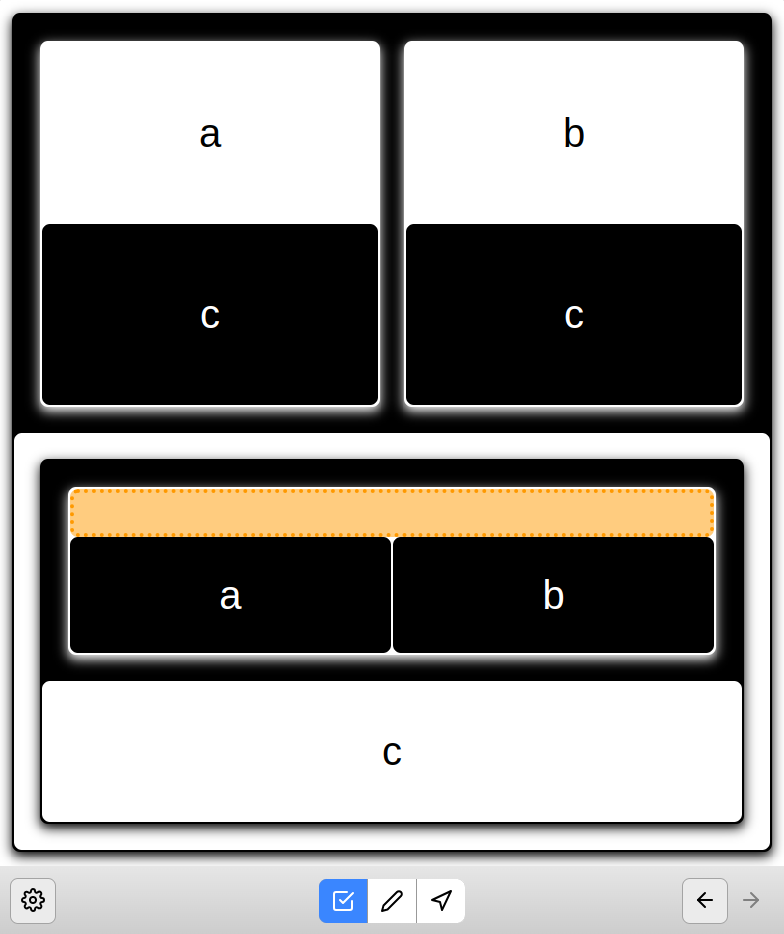
\includegraphics[width=0.7\textwidth]{flower-prover-proof-mode}
  \hspace{1em}
  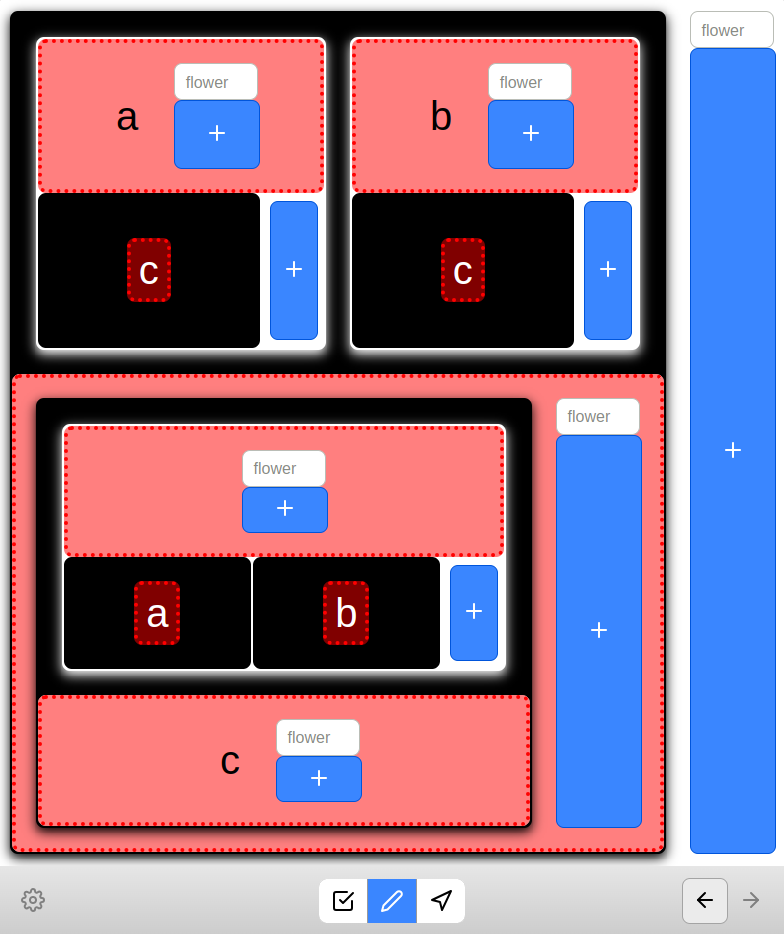
\includegraphics[width=0.7\textwidth]{flower-prover-edit-mode}
  \caption{\Proof mode (left) and \Edit mode (right) of the \kl{Flower\,\,Prover}}
  \labfig{flowers-prover-modes}
\end{figure*}

\paragraph{Modal interface}

The \kl{Flower\,\,Prover} is organized in two main \emph{modes} of interaction,
providing different sets of \kl{direct manipulation} actions on
goals\sidenote{Another example of modal interface is the popular text editor
\texttt{vim}, with its \emph{normal} mode for high-level manipulation of text
through commands and macros, and its \emph{edit} mode for low-level insertion
and deletion of characters.}:
\begin{description}
  \item[\Proof mode] this is the main mode, where \kl{goals} can be proved by
  reducing them to the empty \kl{bouquet} $\emptyset$. It corresponds in purpose to
  the interactive proof mode of modern \kl{proof assistants} like \kl{Coq}, \kl{Lean} and
  \kl{Isabelle}, and to the interactive \kl{proof view} of \kl{Actema}.
  % Indeed, every action in this mode is performed by direct manipulation of
  % flowers through pointing interactions: either clicking on empty areas/gardens,
  % or dragging and dropping flowers into gardens.
  As will be detailed shortly, there is almost a one-to-one correspondence
  between \Proof actions, and the $\Nature$-rules of the \kl{flower calculus}.
  
  \item[\Edit mode] in this mode, the user can construct arbitrary
  flowers by clicking on buttons and filling text fields, or modify the \kl{goal} by
  clicking and dragging flowers around. It corresponds in purpose to the text
  editor used for writing theories in the \emph{vernacular} language of a \kl{proof
  assistant}\sidenote{The term ``vernacular'' was used for the first time in the
  context of \kl{proof assistants} by the founder of the field, N. G. de Bruijn
  \cite{de_bruijn_mathematical_1994}.}. \Edit actions implement exactly the
  $\Culture$-rules of the \kl{flower calculus}.
\end{description}

\begin{remark}
  A nice analogy for these two modes can be found in the video game
  \emph{Minecraft}: the \emph{survival} mode, where the player has to gather and
  craft resources to survive, corresponds to the \Proof mode, where the user has
  to combine and justify existing statements with the \kl{analytic} $\Nature$-rules;
  while the \emph{creative} mode, where the player can build and destroy
  anything instantly with unlimited resources, corresponds to the \Edit mode,
  where the user can insert or delete arbitrary flowers with the (synthetic?)
  $\Culture$-rules.
\end{remark}

\reffig{flowers-prover-modes} shows side-by-side the same \kl{goal} representing the
flower $\flower{(\flower{a}{c}),(\flower{b}{c})}{(\flower{(\flower{}{a \sep
b})}{c})}$, but viewed through the two different modes. At any point during a
proof, the user can switch between the two modes by clicking on the
corresponding button in the \emph{mode selection bar}, located at the bottom of
the screen: \Proof and \Edit modes are mapped respectively to the left button with
a checkmark icon, and the middle button with a pencil icon.

It is also possible to \emph{undo/redo} any action, whichever mode it was done
in, by clicking on the corresponding buttons located on the bottom-right corner
of the screen. This is implemented by a simple stack recording the entire state
of the application, that is updated every time the user performs an action, and
popped/pushed when the user clicks on the undo/redo buttons. Since the
application state includes the current interaction mode, undoing/redoing an
action will automatically switch to the mode in which the action was performed.

\paragraph{\Proof actions}

\begin{table*}[h]
  \def\arraystretch{1.5}


% \hspace{-8em}
\subfloat[\Proof actions\labtab{flowers-proof-actions}]{
% \hspace{-0.1\textwidth}
\begin{tabular}{|c|C{5em}|C{11em}|}
\hline
\textbf{Action} & \textbf{Gesture} & \textbf{$\Nature$-rule} \\ \hline
\intro{Justify} & Click on $a$ & $$\R[\kl{poll{\da}}]{\Xi\select{\phantom{a}}}{\Xi\select{a}}$$ \\ \hline
\intro{Import} & \kl{DnD} of $\phi$ into $\Xi\hole$ & $$\prftree[l][r]{\kl{poll{\ua}}}{$\phi$ non-atomic}{\Xi\select{\phi}}{\Xi\select{\phantom{\phi}}}$$ \\ \hline
\intro{QED} & Click on empty petal & $$\R[\kl{epet}]{}{\flower{\gamma}{\garden{}{} \sep \Delta}}$$ \\ \hline
\intro{EFQ} & Click on empty pistil &
$$
\R[\kl{srep}]
{\R[\kl{epet}]
{}
{\flower{\Phi}{\cdot}}}
{\flower{\Phi, (\flower{\garden{}{}}{})}{\Delta}}
$$
\\ \hline
\intro{Case} & Click on empty pistil & $$\prftree[l][r]{\kl{srep}}{$n \geq 2$}{\flower{\Phi}{\fset{i}{n}{\flower{\gamma_i}{\Delta}}}}{\flower{\Phi, (\flower{\garden{}{}}{\fset{i}{n}{\gamma_i}})}{\Delta}}$$ \\ \hline
\intro{Unlock} & Click on empty pistil & $$\R[\kl{epis{\da}}]{\flower{\Phi, \Psi}{\Delta}}{\flower{\Phi, (\flower{\garden{}{}}{\Psi})}{\Delta}}$$ \\ \hline
\end{tabular}
}
\subfloat[\Edit actions\labtab{flowers-edit-actions}]{
\begin{tabular}{|c|C{7em}|C{7em}|}
\hline
\textbf{Action} & \textbf{Gesture} & \textbf{$\Culture$-rule} \\ \hline
\intro{Grow} & \texttt{Add} button in \kl{positive} bouquet & $$\R[\kl{grow}]{\Xi^+\select{\flower{}{\garden{}{}}}}{\Xi^+\select{\phantom{\flower{}{\garden{}{}}}}}$$ \\ \hline
\intro{Glue} & \texttt{Add} button in \kl{negative} corolla & $$\R[\kl{glue}]{\Xi^-\select{\flower{\gamma}{\garden{}{} \sep \Delta}}}{\Xi^-\select{\flower{\gamma}{\Delta}}}$$ \\ \hline
\intro{Insert} & \texttt{Add} button in grown bouquet/corolla & \kl{grow}/\kl{glue} \\ \hline
\intro{Delete} & Click on grown flower/petal & \kl{grow}/\kl{glue} \\ \hline
\intro{Crop} & Click on \kl{negative} flower & $$\R[\kl{crop}]{\Xi^-\select{\phantom{\phi}}}{\Xi^-\select{\phi}}$$ \\ \hline
\intro{Pull} & Click on \kl{positive} petal & $$\R[\kl{pull}]{\Xi^+\select{\flower{\gamma}{\Delta}}}{\Xi^+\select{\flower{\gamma}{\delta \sep \Delta}}}$$ \\ \hline
\end{tabular}
}

  \caption{Graphical actions of the \kl{Flower\,\,Prover}}
  \labfig{flowers-actions}
\end{table*}

\begin{figure*}[h]
  \newcommand{\incl}[1]{\vcenter{\hbox{\includegraphics[width=0.4\textwidth]{#1}}}}
$$
\hspace{-3em}
\begin{array}{cccccc@{\vspace{1em}}}
&\incl{flowers-prover-anim-0}
&\xstep{\Action{Case}}
&\incl{flowers-prover-anim-1}
&\xstep{\Action{Unlock}}
&\incl{flowers-prover-anim-2}
\\
\xstep{\Action{Import}}
&\incl{flowers-prover-anim-3}
&\xstep{\Action{Import}}
&\incl{flowers-prover-anim-4}
&\xstep{\Action{Justify}}
&\incl{flowers-prover-anim-5}
\\
\xstep{\Action{Unlock}}
&\incl{flowers-prover-anim-6}
&\xstep{\Action{Justify}}
&\incl{flowers-prover-anim-7}
&\xstep{\Action{QED}}
&\incl{flowers-prover-anim-8}
\end{array}
$$
  \caption{A sequence of \Proof actions in the \kl{Flower\,\,Prover}}
  \labfig{flowers-prover-anim}
\end{figure*}

\reftab{flowers-proof-actions} shows the precise mapping of \Proof actions to
$\Nature$-rules, together with the associated gestures for triggering them; and
\reffig{flowers-prover-anim} shows a sequence of screenshots of the \kl{Flower\,\,Prover}, capturing the execution of a sequence of \Proof actions reducing the
\kl{subgoal} $\flower{(\flower{}{a \sep b})}{c}$ to $\flower{b}{c}$. A few
comments are in order:

\begin{description}
  \item[Pollination] The most central actions are those implementing
  the \kl{pollination} rules \kl{poll{\da}} and \kl{poll{\ua}}, called respectively
  \kl{Justify} and \kl{Import}. In fact, they are \emph{less} general
  than those rules: one can only \kl{Justify} flowers that are \emph{atomic}
  by clicking on them, and \kl{Import} \emph{non-atomic} flowers by dragging
  and dropping them at the desired location. We conjecture that these
  restrictions do not jeopardize the completeness of $\Nature$-rules, and
  correspond to the process of $\eta$-expansion in \kl{$\lambda$-calculus}.
  
  \item[Suggestions]
  
  The fourth screenshot in \reffig{flowers-prover-anim} shows the flower $\phi
  \deq \flower{a}{c}$ being dragged in the process of an \kl{Import} action.
  If you look closely, you will notice that there are many areas whose border is
  highlighted with dashed yellow lines: these correspond to all \kl{contexts}
  $\Xi\hole$ where $\phi$ can be imported, i.e. such that
  $\chyp{\phi}{\Xi\hole}$. This is a first form of \emph{suggestion} in the
  \kl{Flower\,\,Prover}, indicating available valid actions to the user through visual
  feedback\sidenote{A similar mechanism is implemented in \kl{Actema}, where subterms
  that are possible drop targets for \kl{DnD} actions are also highlighted (see
  \refsec{validity}).}.

  In fact, every \Proof action has an associated visual cue, guiding interactive
  proof search by suggesting to the user areas of the \kl{goal} where she might want
  to focus her attention. Since every action other than \kl{Import} is
  performed by a \emph{click} gesture, the area that is highlighted corresponds
  precisely to the area that can be clicked for triggering the action: either a
  green box enclosing the justifiable atom for \kl{Justify} actions, an
  orange box covering the empty \kl{pistil} for \kl{EFQ}, \kl{Case} and
  \kl{Unlock} actions, or a green box covering the empty \kl{petal} for
  \kl{QED} actions.
  
  \item[Fencing] We have already mentioned that we suspect that the
  \kl{epis} rule might be \kl{admissible}. However if it is not, one needs a
  corresponding graphical action in \Proof mode. While it is currently not
  implemented, we plan to add a \emph{selection} mechanism that allows the user
  to select a set of flowers in the \kl{goal}. Then, we could add a \kl{Fence}
  action, whose effect is to enclose the selected flowers in a \kl{petal} attached to
  an empty \kl{pistil}. This action could be mapped to a dedicated button in the
  toolbar that is visible only in \Proof mode, and enabled only when the
  selected flowers are juxtaposed in the same garden.
\end{description}

Since every \Proof action implements a $\Nature$-rule, it is guaranteed to be
\emph{\kl{invertible}}: the user never needs to undo a \Proof action in order to
complete a proof, because it always preserves the provability of the \kl{goal}. Of
course it might still be desirable to do so in specific cases, such as
\kl{Import} actions that may create unneeded copies of flowers\sidenote{In
this specific case, one might want to relax the atomic restriction on
\kl{Justify} actions, in order to avoid the recourse to \kl{Undo}
actions, which can only be performed at the top of the history stack.}.

\paragraph{\Edit actions}

\reftab{flowers-edit-actions} shows the precise mapping of \Edit actions to
$\Culture$-rules, together with the associated gestures for triggering them.
Like the edit mode of \texttt{vim}, \Edit actions are used to \emph{insert} and
\emph{delete} arbitrary flowers in the \kl{goal}:
\begin{description}
  \item[Insertion] The main interface mechanism that is currently
  implemented is the \texttt{Add} button: since the \kl{grow} rule allows to
  insert any flower in a \kl{positive} \kl{bouquet} (i.e. add a new \kl{subgoal}, just like the
  \kl(rule){cut} rule in \kl{sequent calculus}), we expose buttons in all the corresponding
  areas (blue ``+'' buttons in \reffig{flowers-prover-modes}), that can be
  clicked to insert a new flower precisely at the location of the button. There
  are two usage scenarios:
  \begin{itemize}
    \item if the user wants to insert an atomic flower, she can enter the name
    of the atom in a text field placed above the button. Clicking on the button
    will then insert an \kl{occurrence} of this atom;
    \item if the user wants to insert a non-atomic flower, she can leave the
    text field empty. Clicking on the button will then insert an empty flower
    with a single \kl{petal}.
  \end{itemize}
  In both cases, the inserted flower is marked internally by the \kl{Flower\,\,Prover}
  with a \texttt{grown} tag: this means that as long as the user does not leave
  \Edit mode, she can perform arbitrary insertions and deletions inside of the
  grown flower, disregarding any \kl{polarity} constraint normally imposed by
  $\Culture$-rules.
  
  Dually, the \kl{glue} rule is implemented by exposing \texttt{Add} buttons in
  all \kl{negative} \kl{corollas}: those have the effect of growing a new empty \kl{petal},
  that can be further edited through arbitrary insertions and deletions.

  Grown flowers/\kl{petals} are distinguished visually by having their border painted
  in blue. Leaving \Edit mode then has the effect of \emph{committing} every
  \Edit action, i.e. removing every \texttt{grown} tag in the entire \kl{goal}. This
  mechanism enables an incremental, step-by-step construction of flowers, that
  is still sound logically with respect to $\Culture$-rules.

  \item[Deletion] Deleting flowers and \kl{petals} is a more straightforward
  process: one just has to click on the corresponding area, which is highlighted
  in red. To avoid overlap, the area of a flower is identified with that of its
  \kl{pistil}. Thus areas subject to deletion are \kl{negative} atoms and flowers
  (\kl{crop} rule), \kl{positive} \kl{petals} (\kl{pull} rule), as well as any area
  marked as \texttt{grown}.
\end{description}

Since every \Edit action implements a $\Culture$-rule, it is guaranteed to be
\emph{non-\kl{invertible}}: the user might need to undo an \Edit action in order to
complete a proof, because it may break the provability of the \kl{goal}.

\paragraph{\Navigation mode}

The reader might have noticed that there is a third button with a navigation
icon on the right of the mode selection bar. It can be used to enter
\emph{\Navigation mode}, the last mode of interaction that we intend to implement
in the future. The idea is that on real-life \kl{goals}, both the size and level of
nesting of flowers will quickly render the interface unusable, both for
reading/understanding the content and structure of \kl{goals}, and manipulating them
through pointing.

The purpose of the \Navigation mode is then to enable the user to \emph{focus} on
a specific \kl{subgoal}, by simply clicking on the corresponding nested flower. This
would make the \kl{subgoal} take up the whole screen, hiding the outer \kl{context} from
view. Dually, it should also be possible to unfocus a previously focused subgoal
--- e.g. by clicking again on it, so that the full tree structure of the goal
can be freely navigated. \kl{Proof-theoretically}, the \Navigation mode implements the
\emph{functoriality} of rules, i.e. the fact that they can be applied in
\kl{contexts} of \emph{arbitrary} \kl{depth}.

\begin{remark}
This way of navigating tree structures represented as nested areas is typical of
\kl{zoomable user interfaces}, a strand of \kl{GUI} that has been developed by
many pioneers in the field of human-computer interaction such as Ivan Sutherland
in his \intro{Sketchpad} system \sidecite{10.1145/800265.810742}, and Alan Kay
in his \intro{Smalltalk} system \sidecite[4em]{goldberg_smalltalk-72_1976}.
\end{remark}

\paragraph{Automation}

The last feature of the \kl{Flower\,\,Prover} that we have implemented is the
\kl{Auto} \Proof action. It is similar in purpose to the \texttt{auto}
tactic of \kl{Coq}, that tries to simplify the \kl{goal} by performing a limited form of
automation. The \kl{Auto} action is mapped to a dedicated button in the
bottom-left corner of the screen, which is only enabled in \Proof mode
(\reffig{flowers-prover-modes}).

The idea is quite simple: since all click actions available to the user are
pre-computed by highlighting the corresponding areas, there can only be a finite
number of them. So why not try to apply them all automatically? Applying a click
action might generate new ones in the resulting \kl{goal}, so we have to perform this
until a fixpoint is reached. This is very much like the \emph{reproduction} and
\emph{decomposition} phases from the \refproc{life} procedure of
\refsec{flowers-search}, except that we also apply the \kl{poll{\da}} rule
(\kl{Justify} actions) wherever possible. The only \Proof action that is not
considered is the only \kl{DnD} action, \kl{Import}. This is not surprising,
since it corresponds to the \kl{poll{\ua}} rule, which is the main source of
complexity in the \kl{pollination phase} of the \refproc{life} procedure,
because of its ability to duplicate flowers of arbitrary size.

In fact, one could fine-tune the level of automation by considering only a
\emph{subset} of all types of click actions. This is already what we do by
default, by leaving the application of \kl{Case} actions to the user. This
is motivated by the fact that the latter can induce an explosion in the size of
the \kl{goal}. One could even leave the configuration of automated action types to
the user with a dedicated interface. This could include an additional option for
executing \kl{Auto} systematically after every (other) \Proof action,
removing the need to click multiple times on the \kl{Auto} button. In this
setting, any proof in the \kl{Flower\,\,Prover} could be reduced to a sequence of
\kl{Import} and \kl{Case} actions.


\subsection{Towards a unified workflow}\labsubsec{flowers-unified}

\paragraph{Theories and goals}

In the \kl{proof view} of modern \kl{proof assistants} like \kl{Coq} and
\kl{Lean}, there is no distinction between local and global
\kl(sequent){contexts}: a \kl{subgoal} will inherit automatically every
hypothesis from its parent \kl{subgoals}, which are flattened into a big
unstructured list. To recreate this distinction and reduce the size of
\kl{goals} to a manageable level, the only interface mechanism offered to the
user is to exit interactive proof mode, and outsource chunks of the local
\kl(sequent){context} as additional global lemmas and definitions in the current
theory file.

Thus the user has to juggle between two different interfaces that manipulate two
distinct data structures: a traditional text editor for modifying
\emph{theories}, and an \kl{IDE} for writing and executing \kl{proof scripts}
that modify \emph{\kl{goals}}, themselves visualized in a separate \kl{proof
view}. This results in a duplication of means to achieve essentially the same
things: for instance, reordering two lemmas will require to cut and paste one of
them in the theory file, while reordering two hypotheses will require the use of
a dedicated \texttt{move} \kl{tactic}. Other examples can be found for renaming
definitions, applying lemmas, constructing functions, etc. Crucially, the two
interfaces cannot communicate straightforwardly with eachother. In fact,
communication is completely one-way: the user can only invoke definitions and
lemmas of the theory from her \kl{proof script}, by referring to their names.

The \kl{Flower\,\,Prover} can theoretically solve this divide, because it works on a
single data structure: flowers represent \emph{at the same time} the current
goal to be proved in \Proof mode, and the theories that are being built in \Edit
mode. Thus there are still two distinct modes/interfaces, but they work in
unison on the same data. The only (major) current limitation, is that we do not
have any way to \emph{save} proved lemmas for later reuse, because proving a
flower amounts to \emph{erasing} it from the current \kl{goal}. In a sense, theories
built in \Edit mode are only \emph{transient}: they live in \emph{working}
memory, and are disposed of as soon as they become justified in \Proof mode;
while we would like them to be \emph{persistent}, recorded in \emph{long-term}
memory along with their justifications (which would stay hidden from the user by
default). We will discuss in \refsec{Conclusion} some research directions that
we envision to achieve the latter. 

\paragraph{Statements and proofs}

Our above example of ``redundant'' manipulations targets \kl{imperative} tactic
languages, but the argument equally applies to more \kl{declarative} languages
like \kl{Isar}: the point is that the \emph{proof} language, be it
\kl{imperative} or \kl{declarative}, is separated both conceptually and through
its available means of interaction from the language of \emph{statements} used
to build theories. And this separation between proofs and statements is a
natural one that is hard to question, since it is rooted in what is arguably the
most important inspiration of formal logic, and also the form in which informal
mathematics present themselves: \emph{natural language}. Indeed, \kl{symbolic}
formulas reproduce the grammatical structure of sentences expressing logical
propositions, and formal proofs reproduce the inferential structure of arguments
built from sequences of sentences.

\paragraph{Context navigation}

After this little conceptual \textit{aparté}, let us come back to the problem of
managing contexts in proofs. In the \kl{Flower\,\,Prover}, the \emph{local} context is
naturally represented as \emph{everything that is displayed on-screen}. This
includes hypotheses that are available from \kl{pistils} at various levels, but also
potentially alternative \kl{goals} (adjacent \kl{petals}) and further \kl{subgoals} (\kl{positively}
nested flowers). Then rather than being segregated in a separate interface (the
text buffer of the theory), the \emph{global} context is simply the
\emph{entire} \kl{goal}. In fact, there is no reason anymore to make a terminological
distinction between \kl{goals} and theories: a \kl{goal} is just a theory that has yet to
be justified, which can itself be identified with a partial proof (or a ``\kl{proof
term} with holes'' in \kl{type-theoretical} parlance)\sidenote{We will come back to
this idea of merging proofs and statements in the same data structure in the
conclusion, when discussing \emph{development calculi} and the
\kl{Curry-Howard correspondence}. Note however that it is already at work in
\emph{dependent} \kl{type theory}, where \kl{proof terms} can freely occur inside
types. This is exemplified in the \kl{Agda} \kl{proof assistant}, where all
manipulations are done directly on the partial proof/program text.}.

It would still be useful to be able to aggregate automatically the set of all
lemmas and definitions (i.e. hypotheses) available in a focused subgoal
$\Phi\select{\phi}$, so that the user does not need to navigate up and down the
goal/proof tree all the time. This can be done with the help of the \kl{pollination}
relation (\refdef{pollination}), by taking the union $\Psi \deq
\compr{\psi}{\chyp{\psi}{\Phi\hole}}$.

In terms of UI, we could then add a so-called \emph{shelf} displayed in all
interaction modes, that exposes the global context $\Psi$ of the current focus
$\Phi\hole$. We anticipate only two kinds of interaction with any flower $\phi$
in the shelf:
\begin{description}
  \item[Pollination (in \Proof mode)] the user can perform an
  \kl{Import} action by dragging $\phi$;
  \item[Jump to definition (in \Navigation mode)] the user can focus on
  the \kl{subgoal} where $\phi$ originates by clicking on $\phi$.
\end{description}

Since the shelf might contain \emph{a lot} of hypotheses, it will be important
to provide efficient ways to \emph{filter} or \emph{search} through its content.
We imagine three main ways of doing so\sidenote{The first two types of filtering
are already available in most \kl{proof assistants}, e.g. the \texttt{Search} command
of \kl{Coq}.}:
\begin{description}
  \item[By name] the user can type the \emph{name} of a hypothesis in a
  search bar. This implies that flowers have the ability to be named by the
  user.
  \item[By structure] the user can specify a \emph{pattern} that must
  be satisfied by all hypotheses in the shelf. A pattern is just a flower that
  contains pattern variables, which can match any flower. Thus patterns might be
  built with the same tools offered in \Edit mode.
  \item[By selection] the user can select subterms of the \kl{goal}, and
  then ask the system to display only hypotheses that can \emph{interact} with
  these subterms. Here we imagine something along the lines of what we did for
  \kl{Actema} (see \refsec{funcs}).
\end{description}


\section{Conclusion}\labsec{Conclusion}

\subsection{Related works}

\paragraph{Intuitionistic EGs}
  
\begin{marginfigure}
  \begin{mathpar}
    \R[\kl{iter}]
      {\flower{\gamma}{\delta \sep \Delta}}
      {\flower{\gamma}{\delta \sep \delta \sep \Delta}}
    \and
    \R[\kl{deit}]
      {\flower{\gamma}{\delta \sep \delta \sep \Delta}}
      {\flower{\gamma}{\delta \sep \Delta}}
  \end{mathpar}
  \caption{(De)iteration rules for \kl{petals}}
  \labfig{flowers-deit-petals}
\end{marginfigure}

In the original \kl{IEGs} system of Oostra, the \kl{srep} rule is replaced by an
extended (de)iteration rule, that allows to duplicate/merge not only identical
flowers, but also identical \emph{\kl{petals}}, under the condition that they are
attached to the same \kl{pistil}\sidenote{``Cualquier lazo puede iterarse adherido
\emph{al mismo corte}'' \cite[p.~46]{oostra_graficos_2010}.} (rules \kl{iter}
and \kl{deit} in \reffig{flowers-deit-petals}). Thus in a sense, (de)iteration
on \kl{petals} is not as \emph{deep} as on whole flowers, where the two identical
flowers can be separated by an arbitrary number of layers; which might seem like
an arbitrary restriction. A posteriori, we rationalize this choice by seeing it
as an attempt to stay close to the original system \kl{Alpha} of Peirce. In
particular, (de)iteration on \kl{petals} is compatible with the quest for
\emph{\kl{illative atomicity}}, where all rules should be expressed in terms of
insertions and omissions (\refsec{atomicity}); while the \kl{srep} rule is not.
In our case, this is justified by our quest for an \emph{\kl{invertible}} calculus
(natural fragment): indeed to simulate \kl{srep} with \kl{petal} (de)iteration, one
also needs the non-\kl{invertible} $\Culture$-rule \kl{crop} (as well as the
$\Culture$-rule \kl{epis{\da}}), as illustrated by the \kl{srep}-free proof of
\reffig{flowers-srep-free}.

\begin{figure}
  \begin{mathpar}
  \prftree[r][d]{\rsf{poll{\ua}}}
  {\prftree[r][d]{\rsf{poll{\da}}}
  {\prftree[r][d]{\rsf{crop}}
  {\prftree[r]{\rsf{iter}}
  {\prftree[r][d]{\rsf{epis{\da}}}
  {\prftree[r]{\rsf{poll{\da}}}
  {\prftree[r]{\rsf{epet}}
  {}
  {\flower{(\flower{a}{c}),(\flower{b}{c}),c}{\garden{}{}}}}
  {\flower{(\flower{a}{c}),(\flower{b}{c}),c}{c}}}
  {\flower{(\flower{a}{c}),(\flower{b}{c}),(\flower{}{(\flower{}{c})})}{c}}}
  {\flower{(\flower{a}{c}),(\flower{b}{c}),(\flower{}{(\flower{}{c}) \sep (\flower{}{c})})}{c}}}
  {\flower{(\flower{a}{c}),(\flower{b}{c}),(\flower{}{(\flower{}{c}), a \sep (\flower{}{c}), b})}{c}}}
  {\flower{(\flower{a}{c}),(\flower{b}{c}),(\flower{}{(\flower{a}{c}), a \sep (\flower{b}{c}), b})}{c}}}
  {\flower{(\flower{a}{c}),(\flower{b}{c}),(\flower{}{a \sep b})}{c}}
\end{mathpar}
% \begin{mathpar}
%   \prftree[r][d]{\rsf{poll{\ua}}}
%   {\prftree[r][d]{\rsf{poll{\da}}}
%   {\prftree[r][d]{\rsf{crop}}
%   {\prftree[r]{\rsf{iter}}
%   {\prftree[r][d]{\rsf{srep}}
%   {\prftree[r]{\rsf{poll{\da}}}
%   {\prftree[r][d]{\rsf{epet}}
%   {}
%   {\flower{(\flower{a}{c}),(\flower{b}{c})}{(\flower{}{(\flower{c}{\garden{}{}})})}}}
%   {\flower{(\flower{a}{c}),(\flower{b}{c})}{(\flower{}{(\flower{c}{c})})}}}
%   {\flower{(\flower{a}{c}),(\flower{b}{c}),(\flower{}{(\flower{}{c})})}{c}}}
%   {\flower{(\flower{a}{c}),(\flower{b}{c}),(\flower{}{(\flower{}{c}) \sep (\flower{}{c})})}{c}}}
%   {\flower{(\flower{a}{c}),(\flower{b}{c}),(\flower{}{(\flower{}{c}), a \sep (\flower{}{c}), b})}{c}}}
%   {\flower{(\flower{a}{c}),(\flower{b}{c}),(\flower{}{(\flower{a}{c}), a \sep (\flower{b}{c}), b})}{c}}}
%   {\flower{(\flower{a}{c}),(\flower{b}{c}),(\flower{}{a \sep b})}{c}}
% \end{mathpar}
  \caption{Simulating the \kl{srep} rule by iterating \kl{petals}}
  \labfig{flowers-srep-free}
\end{figure}

\paragraph{Focusing}

There is a formal connection between the \kl{poll{\ua}} rule of the \kl{flower
calculus}, and the \emph{absorption} rule $[\mathbf{A}]$ of the dyadic system
$\Sigma_2$ of Andreoli, that handles the \kl{focusing} behavior of exponentials in
linear logic \sidecite{andreoli1992}. Indeed, both rules duplicate a formula
available in the (non-linear) \kl{context} of the sequent/location where the rule is
applied, in order to enable further usage of the formula at said location. While
the absorption rule removes the need for permutation-equivalences between proofs
involving the \emph{\kl{contraction}} rule, the identity rule $[I]$ of $\Sigma_2$
removes the need for the \emph{\kl{weakening}} rule by discarding the non-linear
\kl{context} in one go, just as the \kl{epet} rule of the \kl{flower calculus} renders
the \kl{crop} rule \kl{admissible}.

Sonia Marin has noticed the connection between \emph{bipoles} in \kl{focused}
proofs, and the class of geometric/\kl{coherent formulas}, where the former are seen
as a generalization of the latter \sidecite{marin_axioms_2022}. This is to be
related to our own identification of \kl{$n$-ary scrolls}/flowers as a recursive
generalization of \kl{coherent formulas} at the end of \refsec{IEGs}.

Two years earlier, Brock-Nannestad and Ilik had already made some implicit
connections between \kl{focused} proofs and \kl{coherent formulas}, through their
\emph{exponential normal form} for \kl{intuitionistic} formulas based on Tarski's
highschool identities \sidecite{brock-nannestad_intuitionistic_2019}. Quite
remarkably, \kl{first-order} formulas in their exponential normal form have the exact
same structure as flowers
\cite[Definition~4.2]{brock-nannestad_intuitionistic_2019}. However, the \kl{sequent
calculus} \kl{HS} based on them makes the tradeoff opposite to that of the
natural fragment $\Nature$ of the \kl{flower calculus}: every \kl{inference rule} is
\emph{non}-\kl{invertible}, but the calculus is \kl{contraction}-free. One advantage of
this tradeoff is that they can easily show termination of proof search, while we
have not found a terminating procedure yet for the \kl{flower calculus}. The authors
also mention that \kl{HS} could be turned into a \kl{deep inference} calculus in the
style of \kl{G4ip}\sidenote{This is just another name for the system \kl{LJT}
of Dyckhoff already mentioned in \refch{bubbles-symm}.}.

\paragraph{Development calculi}

In \refsec{flowers-prover}, we have seen how the rules of the \kl{flower calculus}
can be understood as a set of (graphical) \kl{tactics} for building partial proofs
interactively. In Chapter 3 of his thesis \sidecite{ayers_thesis}, Ayers calls
such systems \emph{development calculi}. In particular, he presents his own
development calculus inspired by McBride's OL\kl{EGs} system
\sidecite{mcbride_dependently_2000} and G\&G's prover
\sidecite{ganesalingam_fully_2017} called the \texttt{Box} calculus, where both
goals and partial proofs are represented by the same \texttt{Box} data
structure. Once again, \texttt{Box}es seem to share a very similar structure
with flowers, which was here motivated by the need to avoid backtracking by
having the ability to maintain a disjunction of \kl{goals} with so-called
\emph{disjunctive pairs}, corresponding to the \kl{petals} of flowers. The main
difference is that the \texttt{Box} calculus is based on dependent \kl{type theory}
instead of \kl{first-order logic}: this allows to store the partial \kl{proof terms}
inside of the \texttt{Box}es themselves, while this information is lost during
the construction of flowers (but might be reconstructed from the sequence of
graphical actions and the initial \kl{goal}).

Ayers also mentions the category-theoretical treatment of development calculi by
Sterling and Harper \sidecite{sterling_algebraic_2017}, that abstracts from any
particular type of \kl{judgment}. Thus it might be possible to fit the \kl{flower
calculus} into this framework, by identifying the set of flowers $\flowers$ as a
category of \emph{nested \kl{judgments}}\sidenote{Nested \kl{judgments} are already
considered in some recent categorical semantics of \kl{type theory}, and in
particular those in Sterling's thesis \cite{Sterling2022}. See also
\cite{huang2023synthetic} for a (technical) introduction to the subject.}.

\paragraph{Subformula linking}

Our notion of \emph{\kl{vehicle}} (\refdef{vehicle}) takes its terminology from
Girard, who started giving this name to the set of axiom links of a proof
structure in his transcendental syntax\sidenote{Also, it conveys nicely the idea
that the \kl{vehicle} is the fundamental structure that \emph{drives} the proof
search algorithm.} \sidecite{girard_2017}. But the idea of connecting dual
\kl{occurrences} of atoms, and thus forming a graph with an associated adjacency
matrix whose structure can be exploited in proof search, really dates back to
the \emph{connection method} developed independently by Bibel and Andrews in the
1970s \sidecite{Bibel:2009}. Otten and Kreitz have adapted the connection method
to \kl{intuitionistic} logic \sidecite{10.1007/3-540-59338-1_32}, stating that it is
especially well-suited in an interactive theorem proving environment. Thus it
might be instructive to learn from their proof search algorithm to fix ours.

In fact all proof search procedures designed in this thesis, whether for \kl{bubble
calculi} (\refsubsec{bubbles-search}) or the \kl{flower calculus}
(\refsec{flowers-search}), rest on the fundamental observation coming from the
\kl{subformula linking} methodology of Chaudhuri \sidecite{Chaudhuri2013}, that the
construction of proofs in \kl{deep inference} systems can be driven efficiently and
incrementally by the connection of dual atoms. With its \kl{pollination} rules, the
\kl{flower calculus} allows for a particularly elegant implementation of \kl{subformula
linking} that abstracts away from the syntactic bureaucracy of \kl{symbolic}
connectives, as witnessed by the \kl{pollination phase} of our search procedure. In
\refsubsec{bubbles-search}, we sketched some ideas that blur the frontier
between automated and interactive proof search, notably with the so-called
\emph{rule of thumb} which is another manifestation of \kl{subformula linking}. This
integration of automated and interactive aspects is also at work in the \kl{Flower\,\,Prover}, and it would be interesting to investigate further how to incorporate
our drag-and-drop proof \kl{tactic} (\refch{pba}), but also other \kl{symbolic}
manipulation techniques introduced in the first part of this thesis, into the
\kl{iconic} framework of the \kl{Flower\,\,Prover}.

\paragraph{Analyticity}

We have not discussed the rationale behind our notion of \kl{analyticity}, be it
historical or formal arguments explaining its origins, motivations and
consequences. In a recent article \sidecite{bruscoli_analyticity_2019}, Bruscoli
and Guglielmi propose such a detailed discussion around a precise and generic
definition of \kl{analyticity} for \kl{deep inference} \kl{proof systems} (especially
the \kl{calculus of structures}), which at a glance seems to encompass our own
definition. It would be interesting to study more deeply their work, and related
parts of the \kl{deep inference} literature concerned with \kl{analyticity} and its
applications to efficient proof search procedures
\sidecite{kahramanogullari_reducing_2006,lmcs:1089,10.1145/2003476.2003501,chaudhuri:hal-00772420,10.1007/978-3-662-49630-5_23}.

\subsection{Future works}

\paragraph{Metatheory}

In \refsec{Calculus}, we already mentioned the variant $\Nature \setminus
\{\kl{epis}\} \cup \{\kl{crep}\}$ of the natural fragment, that we conjecture
to enjoy both soundness, completeness and a deduction theorem. But these last
two results shall prove particularly harder to prove, and we currently have very
few insights into how to extend the proofs of this chapter to this setting.
Also, this is not withstanding the fact that we do not really see any practical
applications for such results as of yet. Our initial motivation was to show the
admissibility of the \kl{epis} rule, because it never appears in concrete
proofs. But if this requires adding the \kl{crep} rule instead, then it greatly
reduces the pratical interest of the whole endeavor, since the \kl{crep} rule
does not look particularly well-suited to either automated or interactive
theorem proving.

Another line of research would concern properties of \emph{locality}, in the
sense coined by the \kl{deep inference} community with systems like \kl{SKS} (see
\refsec{eg-completeness}). As mentioned in \refsec{flowers-prover}, we
conjecture that the \kl{poll{\da}} and \kl{poll{\ua}} rules can be restricted
respectively to atomic and non-atomic flowers. But this is less satisfying than
in the \kl{calculus of structures}, where one component of \kl{poll{\ua}}, the
duplicating \emph{\kl{contraction}} rule, can be restricted to atomic formulas. This
probably comes from the fact that \kl{poll{\ua}} also serves the purpose of
\emph{moving} flowers deeper, as witnessed by the \kl{DnD} \kl{Import} action of
the \kl{Flower\,\,Prover}: in the \kl{calculus of structures}, this role is fulfilled by
\emph{switch} rules, which cannot be restricted to atomic structures. The only
solution might be to \emph{simulate} a local \kl{calculus of structures} for
\kl{intuitionistic} logic, like the system \kl{ISp} of Tiu
\sidecite{tiu_local_2006}.

Lastly, it would be interesting to exhibit an \emph{internal}, syntactic
procedure for eliminating cultural $\Culture$-rules in proofs, just like Gentzen
showed \kl{cut-elimination} in \kl{sequent calculus}\sidenote{A sort of
\emph{cult}-elimination, so to speak.}. In this work we preferred a more
semantic approach, because it was simpler and at the right level of abstraction
for our needs. We might be able to take some inspiration from the
\kl{cut-elimination} proofs of \kl{calculi of structures}, which are indeed notoriously
involved.

\paragraph{Automated proof search}

We shall investigate the current sources of non-termination and incompleteness
for our \refproc{life} proof search procedure, through further testing on the
ILTP dataset. If we succeed in passing all tests, the natural continuation will
be to provide formal proofs of termination and completeness. A follow-up
direction would be to extend our algorithm to the \kl{first-order} setting by adding
heuristics for handling \kl{sprinklers}, thus losing completeness.

Another direction of research would consist in comparing our algorithm to
existing search procedures for \kl{EGs}, in particular one that was originally
developed by Peirce, and described by Oostra in \sidecite{oostra_advances_2022}.

\paragraph{Curry-Howard}

We have begun to sketch some ideas for a \kl{Curry-Howard correspondence}, where
flowers and \Proof actions for justifying them ($\Nature$-rules) are identified
respectively with \emph{normal} and \emph{neutral} \kl{terms} of the simply-typed
\kl{$\lambda$-calculus}. For instance, the computational counterpart of the rule
\kl{poll{\da}} in \kl{pistils} would be a kind of \emph{function application}
expressed by the following \kl{app} rule, which is highly reminiscent of the
instantiation rule \kl{ipis}:
$$
\R[\kl{app}]
  {\Xi\select{t~u : (\flower{\subst{\Phi}{u}{x}}{\subst{\Delta}{u}{x}})}}
  {\Xi\select{t : (\flower{\Phi, x : \phi}{\Delta})}}
$$
Given a flower $\phi$ and a neutral \kl{term} $t$, i.e. an $n$-ary function
application of the form $x~t_1 \ldots t_n$, the expression $t : \phi$ is a
\emph{\kl{term} annotation}, that should be read in context as ``this \kl{occurrence} of
$\phi$ is justified by $t$''. Interestingly, $\phi$ itself may contain \kl{term}
annotations, mimicking the fact that normal and neutral \kl{terms} can be defined by
mutual recursion. Then in the \kl{app} rule, we do not just erase the formula
$\phi$ as in the \kl{poll{\da}} rule, but also keep track of the flow of
information by appending the argument $u$ to the justification $t$ (where
$\chyp{(u : \phi)}{\Xi\hole}$), and substituting $u$ to every \kl{occurrence} of the
hypothetical justification $x$ of $\phi$ in $\Phi$ and $\Delta$.

As of now the syntax of annotated flowers is not yet stable, and it is unclear
what would be the computational interpretation of flowers with $n \not= 1$
\kl{petals}. In particular for disjunctive flowers ($n > 1$), it seems that we are
closer to a notion of non-deterministic or parallel computation, than to the
usual branching computation of sum or inductive \kl{types}.

If our intuition is right, then the fact that flowers correspond to (normal)
\kl{$\lambda$-terms} would embody syntactically a recent motto from Miquel stemming
from his study of the foundations of \kl{forcing} and realizability in
implicative
algebras, where ``elements can be seen both as truth values and as (generalized)
realizers, thus \textbf{blurring the frontier between proofs and
types}''\sidenote{Another recent, related incarnation of this phenomenon is the
correspondence uncovered by Haydon between a linear version of \kl{EGs} already
appearing in Peirce's writings, and the proof nets of Girard for linear logic
\cite{haydon_eg_pn}.} \sidecite{miquel_implicative_2020}. Or as he put it in a
recent talk \cite{miquel_implicative_topos_2022}, we get the ultimate
Curry-Howard identification:
$$
\text{\textbf{Realizer}} = \text{\textbf{Program}} = \text{\textbf{Formula}} = \text{\textbf{Type}}
$$
This could also form the basis for further studies on the connections between
\kl{EGs} and (dependent) \kl{type theory}, and ultimately lead to a tight
integration of the \kl{Flower\,\,Prover} with \kl{proof assistants} based on the
latter such as \kl{Coq}, \kl{Lean} and \kl{Agda}. Existing explorations of the
links between \kl{type theory} and \kl{deep inference} include, in historical
order:
\begin{itemize}
  \item a first attempt by Brünnler and McKinnley to devise a \kl{Curry-Howard
  correspondence} for a simple \kl{intuitionistic} \kl{deep inference} calculus with
  conjunction and implication \sidecite{cervesato_algorithmic_2008};
  \item the thesis of Nicolas Guenot, and more precisely the part on "Nested
  Proofs as Programs" where he gives a correspondence between simply-typed
  \kl{$\lambda$-calculi} with explicit substitutions at one end, and calculi of
  structures (Chapter 6) and \kl{nested sequent} calculi (Chapter 5) for the
  implicational fragment of \kl{intuitionistic} logic at the other end
  \cite{guenot_nested_2013};
  \item the atomic \kl{$\lambda$-calculus}, a simply-typed \kl{$\lambda$-calculus} with
  explicit sharing that has a \kl{Curry-Howard correspondence} with proofs in the
  formalism of \emph{open deduction} \sidecite{gundersen_atomic_2013};
  \item a \kl{type} system for interaction nets based on a \kl{calculus of structures} for
  Multiplicative Exponential Linear Logic \sidecite{gimenez_structure_2013};
  \item the thesis of Fanny He, that explores a \kl{classical} variant of the atomic
  \kl{$\lambda$-calculus} based on Saurin's $\Lambda\mu$-calculus
  \sidecite{he_fanny_thesis};
  \item the \emph{spinal} atomic \kl{$\lambda$-calculus}, an extension and
  improvement on the atomic \kl{$\lambda$-calculus} based on a computational
  interpretation of the \emph{switch} rule \sidecite{goubault-larrecq_spinal_2020};
  \item the \emph{collection calculus} that subsumes resource,
  intersection-typed and simply-typed \kl{$\lambda$-calculi}, with a \kl{type} system
  again in open deduction \sidecite{guerrieri_deep_2021};
  \item Ongoing research by Kaustuv Chaudhuri to extend \kl{subformula linking} to
  dependent \kl{type theory}\sidenote{Private communication.}.
\end{itemize}
The work of Guenot on computational interpretations of \kl{nested sequent} calculi
seems closest to the syntax of flowers. Indeed, \kl{nested sequents} are variadic by
nature, and his version of \kl{nested sequents} in particular exploits the
possibility to have \emph{negative} \kl{occurrences} of sequents. Combined with the
dependently-typed \texttt{Box}es of Ayers mentioned earlier (which cannot be
nested negatively), this should provide great insights for the powerful,
dependently-typed version of the \kl{flower calculus} that we seek for.

\paragraph{Flower Prover}

We have already described many features in \refsec{flowers-prover} that we
intend to implement in the future. This includes the \Navigation mode, the
ability to \emph{select} flowers, the \kl{Fence} \Proof action, and the
\emph{shelf} mechanism.

The next step would be to support \kl{first-order} reasoning by adding \kl{sprinklers} and
\kl{first-order} terms, and devising graphical actions for the rules $\{\kl{ipis},
\kl{ipet}\}$ in \Proof mode, and $\{\kl{apis}, \kl{apet}\}$ in \Edit mode.

Last but not least, we want to provide a way to \emph{save} proved lemmas along
with their proof, so that they can be reused and read statically. This will be
crucial for \emph{\kl{proof evolution}}\sidenote{See also
\refsubsec{proof-evolution}.}, and will probably rely on the computational,
dependently-typed version of the \kl{flower calculus} sketched above, where \kl{proof
terms} can appear inside flowers.

\subsection{Theory vs. Practice}

Finally, it should be noted that Peirce did not think of \kl{EGs} as a calculus that
could aid in performing reasoning \emph{per se}, but rather as a tool for
analyzing the finer structure of logical endeavor
\cite[pp.~110--111]{Roberts+1973}:
\begin{quote}
  [...] the purpose which the system was designed to fulfill was ``to enable us
to separate reasoning into its smallest steps so that each one may be examined
by itself'' (Ms 455, p.~2). The aim was not to facilitate reasoning, but to
facilitate the study of reasoning.
\end{quote}

The various achievements presented in this chapter incite us to depart from this
conception. Indeed, our particular viewpoint on the \kl{illative transformations},
that emphasizes \kl{goal}-reduction through \kl{invertible} and \kl{analytic}
rules, enabled us to design a novel and promising type of graphical interface
for interactive proof building, which integrates easily and elegantly some
(limited) forms of automation. This was also made possible by the use of
variables instead of \kl{lines of identity}, trading a heavy graphical apparatus
with local \kl{inference rules} for a simple, well-known textual syntax with
complex (but automated) global dynamics in the form of \kl{substitutions}. Hence
we believe the \emph{opposite}, that \kl{EGs} \emph{can} form the basis for an
ergonomic calculus of logical deduction, in addition to being a powerful tool
for meta-logical analysis.


\end{scope}


\appendix % From here onwards, chapters are numbered with letters, as is the appendix convention

\pagelayout{wide} % No margins
\addpart{Appendix}
\pagelayout{margin} % Restore margins

% \setchapterpreamble[u]{\margintoc}
\chapter{Standard Proof Calculi}
\labch{app:calculi}


% \setchapterpreamble[u]{\margintoc}
\chapter{Symmetric Bubble Calculi}
\labch{app:bubbles-symm}

\begin{scope}\knowledgeimport{bubble}
\begin{scope}\knowledgeimport{symm}

\section{Soundness}\labsec{app:bubbles-soundness}

\begin{lemma}[Generalized weakening]\lablemma{app:bubbles-weakening}
  $\psint{S} \sement{} \psint{S \mix (\Gamma \seq \Delta)}$.
\end{lemma}
\begin{proof}
  Let $S = \Gamma' \J \Delta'$. We proceed by induction on $\sdepth{\J}$.
  \begin{itemize}
    \item[\bcase]
    $$
    \begin{array}{rcll}
      \psint{\Gamma' \seq \Delta'}
      &=& \nsint{\Gamma} \limp \psint{\Delta} & \\
      &\sement{}& \nsint{\Gamma} \limp \psint{\Delta} \lor \psint{\Delta'} & \\
      &\sement{}& \nsint{\Gamma'} \wedge \nsint{\Gamma} \limp \psint{\Delta} \lor \psint{\Delta'} & \\
      &=& \psint{\Gamma', \Gamma \seq \Delta, \Delta'} & \\
    \end{array}
    $$
    \item[\rcase]
    $$
    \begin{array}{rcll}
      \psint{\Gamma' \piq{\cS} \Delta'}
      &=& \bigwedge_{T \in \cS}{\psint{T \mix (\Gamma' \seq \Delta')}} & \\
      &\sement{}& \bigwedge_{T \in \cS}{\psint{(T \mix (\Gamma' \seq \Delta')) \mix (\Gamma \seq \Delta)}} &\text{(IH)} \\
      &=& \bigwedge_{T \in \cS}{\psint{T \mix ((\Gamma' \seq \Delta') \mix (\Gamma \seq \Delta))}} & \\
      &=& \bigwedge_{T \in \cS}{\psint{T \mix (\Gamma', \Gamma \seq \Delta, \Delta')}} & \\
      &=& \psint{\Gamma', \Gamma \piq{\cS} \Delta, \Delta'} & \\
    \end{array}
    $$
  \end{itemize}
\end{proof}

\begin{lemma}[Generalized contraction]\lablemma{app:bubbles-contraction}
  $\psint{S \mix (\seq I, I)} \semequiv{} \psint{S \mix (\seq I)}$ and
  $\psint{S \mix (I, I \seq)} \semequiv{} \psint{S \mix (I \seq)}$.
\end{lemma}
\begin{proof}
  Let $S = \Gamma \J \Delta$. We proceed by induction on $\sdepth{\J}$.
  \begin{itemize}
    \item[\bcase]
    $$
    \begin{array}{rcll}
      \psint{\Gamma \seq I, I, \Delta}
      &=& \nsint{\Gamma} \limp (\psint{I} \land \psint{I}) \vee \psint{\Delta} & \\
      &\semequiv& \nsint{\Gamma} \limp \psint{I} \vee \psint{\Delta} &\text{(\reffact{idempotency})} \\
      &=& \psint{\Gamma \seq I, \Delta} & \\
    \end{array}
    $$
    $$
    \begin{array}{rcll}
      \psint{\Gamma, I, I \seq \Delta}
      &=& \nsint{\Gamma} \land (\nsint{I} \land \nsint{I}) \limp \psint{\Delta} & \\
      &\semequiv& \nsint{\Gamma} \land \nsint{I} \limp \psint{\Delta} &\text{(\reffact{idempotency})} \\
      &=& \psint{\Gamma, I \seq \Delta} & \\
    \end{array}
    $$
    \item[\rcase]
    $$
    \begin{array}{rcll}
      \psint{\Gamma \piq{\cS} I, I, \Delta}
      &=& \bigwedge_{T \in \cS}{\psint{T \mix (\Gamma \seq I, I, \Delta)}} & \\
      &=& \bigwedge_{T \in \cS}{\psint{(T \mix (\Gamma \seq \Delta)) \mix (\seq I, I)}} & \\
      &=& \bigwedge_{T \in \cS}{\psint{(T \mix (\Gamma \seq \Delta)) \mix (\seq I)}} &\text{(IH)} \\
      &=& \bigwedge_{T \in \cS}{\psint{T \mix (\Gamma \seq I, \Delta)}} & \\
      &=& \psint{\Gamma \piq{\cS} I, \Delta} & \\
    \end{array}
    $$
    $$
    \begin{array}{rcll}
      \psint{\Gamma, I, I \piq{\cS} \Delta}
      &=& \bigwedge_{T \in \cS}{\psint{T \mix (\Gamma, I, I \seq \Delta)}} & \\
      &=& \bigwedge_{T \in \cS}{\psint{(T \mix (\Gamma \seq \Delta)) \mix (I, I \seq)}} & \\
      &=& \bigwedge_{T \in \cS}{\psint{(T \mix (\Gamma \seq \Delta)) \mix (I \seq)}} &\text{(IH)} \\
      &=& \bigwedge_{T \in \cS}{\psint{T \mix (\Gamma, I \seq \Delta)}} & \\
      &=& \psint{\Gamma, I \piq{\cS} \Delta} & \\
    \end{array}
    $$
  \end{itemize}
\end{proof}

\begin{lemma}[Generalized weak distributivity]\lablemma{app:bubbles-weakdistrib}
  \begin{align}
    \psint{\Gamma \J \Delta} \lor \psint{I} &\sement{} \psint{\Gamma \J I, \Delta} \label{app:eqn:weakdistrib-one} \\
    \psint{\Gamma \J I, \Delta} &\sementC \psint{\Gamma \J \Delta} \lor \psint{I} \label{app:eqn:weakdistrib-two} \\
    \nsint{\Gamma, I \J \Delta} &\sementB \nsint{I} \land \nsint{\Gamma \J \Delta} \label{app:eqn:weakdistrib-three} \\
    \nsint{I} \land \nsint{\Gamma \J \Delta} &\sementC \nsint{\Gamma, I \J \Delta} \label{app:eqn:weakdistrib-four}
  \end{align}
\end{lemma}
\begin{proof}
  We only prove (\ref{app:eqn:weakdistrib-one}): the proof of
  (\ref{app:eqn:weakdistrib-two}) is the same, except that we use the converse
  inequality of \reffact{weakdistrib} that holds in \kl{Boolean algebras}.
  (\ref{app:eqn:weakdistrib-three}) and (\ref{app:eqn:weakdistrib-four}) hold by duality
  from (\ref{app:eqn:weakdistrib-one}) and (\ref{app:eqn:weakdistrib-two}), i.e. for
  (\ref{app:eqn:weakdistrib-three}) we have
  $$
  \def\arraystretch{2.5}
  \begin{array}{rrcll}
               & \psint{\soldual{\Delta} \mathbin{\soldual{\J}} \soldual{\Gamma}} \lor \psint{\soldual{I}} &\sement{}& \psint{\soldual{\Delta} \mathbin{\soldual{\J}} \soldual{I}, \soldual{\Gamma}} &\text{(\ref{app:eqn:weakdistrib-one})} \\
    \text{iff} & \soldual{\psint{\soldual{\Delta} \mathbin{\soldual{\J}} \soldual{I}, \soldual{\Gamma}}} &\sementB& \soldual{\psint{\soldual{\Delta} \mathbin{\soldual{\J}} \soldual{\Gamma}} \lor \psint{\soldual{I}}} &\text{(\reffact{duality})} \\
    \text{iff} & \nsint{\soldual{\soldual{\Gamma}}, \soldual{\soldual{I}} \mathbin{\soldual{\soldual{{\J}}}} \soldual{\soldual{\Delta}}} &\sementB& \nsint{\soldual{\soldual{\Gamma}} \mathbin{\soldual{\soldual{{\J}}}} \soldual{\soldual{\Delta}}} \land \nsint{\soldual{\soldual{I}}} &\text{(\reflemma{int-duality})} \\
    \text{iff} & \nsint{\Gamma, I \mathbin{\J} \Delta} &\sementB& \nsint{\Gamma \mathbin{\J} \Delta} \land \nsint{I} &\text{(\reflemma{involutivity})} \\
  \end{array}
  $$
  We prove (\ref{app:eqn:weakdistrib-one}) by induction on $\sdepth{\J}$.
  \begin{itemize}
    \item[\bcase]
    $$
    \begin{array}{rcll}
      \psint{\Gamma \seq \Delta} \lor \psint{I}
      &=& \left(\nsint{\Gamma} \limp \psint{\Delta}\right) \lor \psint{I} & \\
      &\sement{}& \nsint{\Gamma} \limp \psint{\Delta} \lor \psint{I} &\text{(\reffact{weakdistrib})} \\
      &=& \psint{\Gamma \seq I, \Delta} & \\
    \end{array}
    $$
    \item[\rcase]
    $$
    \begin{array}{rcll}
      \psint{\Gamma \piq{\cS} \Delta} \lor \psint{I}
      &=& \psintAndMix{(\Gamma' \JB \Delta')}{\cS}{\Gamma}{\Delta} \lor \psint{I} & \\
      &=& \psintAnd{(\Gamma' \JB \Delta')}{\cS}{\Gamma, \Gamma' \JB \Delta', \Delta} \lor \psint{I} & \\
      &\semequiv{\Lattice}& \psintAnd{(\Gamma' \JB \Delta')}{\cS}{\Gamma, \Gamma' \JB \Delta', \Delta} \lor \psintAnd{(\Gamma' \JB \Delta')}{\cS}{I} &\text{(\reffact{idempotency})} \\
      &\semequiv{\Lattice}& \bigwedge_{(\Gamma' \JB \Delta') \in \cS}{\left(\psint{\Gamma, \Gamma' \JB \Delta', \Delta} \lor \psint{I}\right)} &\text{(\reffact{distributivity})} \\
      &\sement{}& \bigwedge_{(\Gamma' \JB \Delta') \in \cS}{\left(\psint{\Gamma, \Gamma' \JB I, \Delta', \Delta} \right)} &\text{(IH)} \\
      &=& \psintAndMix{(\Gamma' \JB \Delta')}{\cS}{\Gamma}{I, \Delta} & \\
      &=& \psint{\Gamma \piq{\cS} I, \Delta} & \\
    \end{array}
    $$
  \end{itemize}
\end{proof}

\begin{lemma}[Generalized currying]\lablemma{app:bubbles-currying}
  \begin{align}
    \psint{\Gamma, I \J \Delta} &\semequiv{} \nsint{I} \limp \psint{\Gamma \J \Delta} \label{app:eqn:currying-one} \\
    \nsint{\Gamma \J I, \Delta} &\semequiv{\Brouwer} \nsint{\Gamma \J \Delta} \lsub \psint{I} \label{app:eqn:currying-two}
  \end{align}
\end{lemma}
\begin{proof}
  We only prove (\ref{app:eqn:currying-one}), as (\ref{app:eqn:currying-two}) holds by
  duality as in \reflemma{bubbles-weakdistrib}. We proceed by induction on
  $\sdepth{\J}$.
  \begin{itemize}
    \item[\bcase]
    $$
    \begin{array}{rcll}
      \psint{\Gamma, I \seq \Delta}
      &=& \nsint{\Gamma} \land \nsint{I} \limp \psint{\Delta} & \\
      &\semequiv& \nsint{I} \land \nsint{\Gamma} \limp \psint{\Delta} &\text{(\reffact{lattice-commutativity})} \\
      &\semequiv& \nsint{I} \limp \nsint{\Gamma} \limp \psint{\Delta} &\text{(\reffact{currying})} \\
      &=& \nsint{I} \limp \psint{\Gamma \seq \Delta} & \\
    \end{array}
    $$
    \item[\rcase]
    $$
    \begin{array}{rcll}
      \psint{\Gamma, I \piq{\cS} \Delta}
      &=& \psintAndMix{(\Gamma' \JB \Delta')}{\cS}{\Gamma, I}{\Delta} & \\
      &=& \psintAnd{(\Gamma' \JB \Delta')}{\cS}{\Gamma', \Gamma, I \JB \Delta, \Delta'} & \\
      &\semequiv& \bigwedge_{(\Gamma' \JB \Delta') \in \cS}{\left(\nsint{I} \limp \psint{\Gamma', \Gamma \JB \Delta, \Delta'}\right)} &\text{(IH)} \\
      &\semequiv& \nsint{I} \limp \bigwedge_{(\Gamma' \JB \Delta') \in \cS}{\psint{\Gamma', \Gamma \JB \Delta, \Delta'}} &\text{(\reffact{distributivity})} \\
      &=& \nsint{I} \limp \bigwedge_{(\Gamma' \JB \Delta') \in \cS}{\psint{(\Gamma' \JB \Delta') \mix (\Gamma \seq \Delta)}} & \\
      &=& \nsint{I} \limp \psint{\Gamma \piq{\cS} \Delta} & \\
    \end{array}
    $$
  \end{itemize}
\end{proof}

\begin{lemma}[Local soundness]\lablemma{app:bubbles-local-soundness}
  
  If $S \lstep{} T$ then $\psint{T \mix (\Gamma \seq \Delta)} \sementC \psint{S
  \mix (\Gamma \seq \Delta)}$.
\end{lemma}
\begin{proof}
  We show that $S \lstep{} T$ implies $\psint{T} \sementC \psint{S}$ by inspection
  of each rule of \kl{system~B}. That we can mix an arbitrary top-level \kl(sequent){context}
  $\Gamma \seq \Delta$ into $S$ and $T$ follows from \reffact{bubbles-top-level}.

  \def\arraystretch{1.25}
  \begin{itemize}
    \item[\kl{i{\da}}]
    $$
    \begin{array}{rcll}
      \psint{\Gamma \piq{} \Delta}
      &=& \bigwedge_{U \in \emptyset}{\psint{U \mix (\Gamma \seq \Delta)}} &\\
      &=& \top & \\
      &\semequiv& \nsint{\Gamma} \wedge A \limp A \lor \psint{\Delta} &\\
      &=& \psint{\Gamma, A \seq A, \Delta}
    \end{array}
    $$
    \item[\kl{i{\ua}}]
    $$
    \begin{array}{rcll}
      \psint{\Gamma \piq{\seq A \sep A \seq} \Delta}
      &=& \psint{\Gamma \seq A, \Delta} \wedge \psint{\Gamma, A \seq \Delta} & \\
      &=& (\nsint{\Gamma} \limp A \lor \psint{\Delta}) \land (\nsint{\Gamma} \land A \limp \psint{\Delta}) & \\
      &\semequiv& (\nsint{\Gamma} \limp A \lor \psint{\Delta}) \wedge (\nsint{\Gamma} \limp A \limp \psint{\Delta}) &\text{(\reffact{currying})}\\
      &\semequiv& \nsint{\Gamma} \limp (A \lor \psint{\Delta}) \wedge (A \limp \psint{\Delta}) &\text{(\reffact{distributivity})}\\
      &\semequiv& \nsint{\Gamma} \limp \psint{\Delta} &\text{(\reffact{gencut})}\\
      &=& \psint{\Gamma \seq \Delta} & \\
    \end{array}
    $$
    \item[{\kl{w{-}}}, {\kl{w{+}}}] By \reflemma{bubbles-weakening}.
    \item[{\kl{c{-}}}, {\kl{c{+}}}] By \reflemma{bubbles-contraction}.

    % Soundness of membrane rules for non-empty bubbles instead of bubble
    % swapping rules. Pro: invertible. Con: completeness might be harder to
    % prove.

    % \item[{\kl{s{-}}}, {\kl{s{+}}}] We only write the proof for
    % {\kl{s{-}}}, the proof for {\kl{s{+}}} is symmetric. We proceed by
    % induction on $\sdepth{\J}$.
    % \begin{itemize}
    %   \item[\bcase]
    %   $$
    %   \begin{array}{rcll}
    %     \psint{\piq{S \seq} \mix \Gamma \seq \Delta}
    %     &=& \psint{\Gamma \piq{S \seq} \Delta} & \\
    %     &=& \psint{\Gamma, S \seq \Delta} & \\
    %     &=& \nsint{\Gamma} \wedge \nsint{S} \limp \psint{\Delta} & \\
    %     &=& \nsint{\Gamma} \wedge \nsint{\piq{S}} \limp \psint{\Delta} & \\
    %     &=& \psint{\Gamma, (\piq{S}) \seq \Delta} & \\
    %   \end{array}
    %   $$
    %   \item[\rcase]
    %   $$
    %   \begin{array}{rcll}
    %     \psint{\piq{S \seq} \mix \Gamma \piq{\cS} \Delta}
    %     &=& \psint{\Gamma \piq{\cS \sep S \seq} \Delta} & \\
    %     &=& \bigwedge_{T \in \cS}{\psint{T \mix (\Gamma \seq \Delta)}} \land \psint{\Gamma, S \seq \Delta} & \\
    %     &=& \bigwedge_{T \in \cS}{\psint{T \mix (\Gamma \seq \Delta)}} \land \psint{(\Gamma \seq \Delta) \mix (S \seq)} & \\
    %     &\semequiv& \bigwedge_{T \in \cS}{\psint{T \mix (\Gamma \seq \Delta)}} \land \bigwedge_{T\in\cS}{\psint{(\Gamma \seq \Delta) \mix (S \seq)}} & \\
    %     &\sement{}& \bigwedge_{T \in \cS}{\psint{T \mix (\Gamma \seq \Delta) \mix (\Gamma \seq \Delta) \mix (S \seq)}} &\text{(\reflemma{bubbles-mix})} \\
    %     &\semequiv& \bigwedge_{T \in \cS}{\psint{T \mix (\Gamma \seq \Delta) \mix (S \seq)}} &\text{(\reflemma{bubbles-contraction})} \\
    %     &\sement{}& \bigwedge_{T \in \cS}{\psint{T \mix (\Gamma \seq \Delta) \mix \piq{S \seq}}} &\text{(\reflemma{bubbles-piq})} \\
    %     &=& \bigwedge_{T \in \cS}{\psint{\piq{S \seq} \mix ((\Gamma \seq \Delta) \mix T)}} & \\
    %     &=& \bigwedge_{(\Gamma' \JB \Delta') \in \cS}{\psint{\piq{S \seq} \mix ((\Gamma \seq \Delta) \mix (\Gamma' \JB \Delta'))}} & \\
    %     &=& \bigwedge_{(\Gamma' \JB \Delta') \in \cS}{\psint{\piq{S \seq} \mix (\Gamma', \Gamma \JB \Delta, \Delta')}} & \\
    %     &\sement{}& \bigwedge_{(\Gamma' \JB \Delta') \in \cS}{\psint{\Gamma', \Gamma, (\piq{S}) \JB \Delta, \Delta'}} &\text{(IH)} \\
    %     &=& \bigwedge_{(\Gamma' \JB \Delta') \in \cS}{\psint{(\Gamma' \JB \Delta') \mix (\Gamma, (\piq{S}) \seq \Delta)}} & \\
    %     &=& \psint{\Gamma, (\piq{S}) \piq{\cS} \Delta} & \\
    %   \end{array}
    %   $$
    % \end{itemize}

    \item[{\kl{f{\ua}}}]
    $$
    \begin{array}{rcll}
      \psint{\Gamma \piq{\cS \sep \Gamma' \piq{\cS'} \Delta' \sep S} \Delta}
      &=& \psintAndMix{T}{\cS}{\Gamma}{\Delta} \land \psint{\Gamma, \Gamma' \piq{\cS'} \Delta', \Delta} \land \psint{S \mix (\Gamma \seq \Delta)} & \\
      &\sement{}& \psintAndMix{T}{\cS}{\Gamma}{\Delta} \land \psint{\Gamma, \Gamma' \piq{\cS'} \Delta', \Delta} \land \psint{S \mix (\Gamma, \Gamma' \seq \Delta', \Delta)} &\text{(\reflemma{bubbles-weakening})} \\
      &=& \psint{\Gamma \piq{\cS \sep \Gamma' \piq{\cS' \sep S} \Delta'} \Delta} & \\
    \end{array}
    $$

    \item[{\kl{f{-}{\da}}}]
    $$
    \begin{array}{rcll}
      \psint{\Gamma \piq{\Gamma', I \JB \Delta' \sep \cS} \Delta}
      &=& \psint{\Gamma, \Gamma', I \JB \Delta', \Delta} \land \bigwedge_{S \in \cS}{\psint{S \mix (\Gamma \seq \Delta)}} & \\
      &=& \psint{\Gamma, I \piq{\Gamma' \JB \Delta' \sep \cS} \Delta} & \\
    \end{array}
    $$
    \item[{\kl{f{+}{\da}}}]
    $$
    \begin{array}{rcll}
      \psint{\Gamma \piq{\cS \sep \Gamma' \JB I, \Delta'} \Delta}
      &=& \bigwedge_{S \in \cS}{\psint{S \mix (\Gamma \seq \Delta)}} \land \psint{\Gamma, \Gamma' \JB I, \Delta', \Delta} & \\
      &=& \psint{\Gamma \piq{\cS \sep \Gamma' \JB \Delta'} I, \Delta} & \\
    \end{array}
    $$
    \item[{\kl{f{-}{+}{\da}}}]
    We show that $\psint{\Gamma \J (\Gamma', I \JB \Delta'), \Delta} \sement{}
    \psint{\Gamma, I \J (\Gamma' \JB \Delta'), \Delta}$ by induction on
    $\sdepth{\J}$.
    \begin{itemize}
      \item[\bcase]
      $$
      \begin{array}{rcll}
        \psint{\Gamma \seq (\Gamma', I \JB \Delta'), \Delta}
        &=& \nsint{\Gamma} \limp \psint{\Gamma', I \JB \Delta'} \lor \psint{\Delta} & \\
        &\semequiv& \nsint{\Gamma} \limp \left(\nsint{I} \limp \psint{\Gamma' \JB \Delta'}\right) \lor \psint{\Delta} &\text{(\reflemma{bubbles-currying})} \\
        &\sement{}& \nsint{\Gamma} \limp \left(\nsint{I} \limp \psint{\Gamma' \JB \Delta'} \lor \psint{\Delta}\right) &\text{(\reffact{weakdistrib})} \\
        &\semequiv& \nsint{\Gamma} \land \nsint{I} \limp \psint{\Gamma' \JB \Delta'} \lor \psint{\Delta} &\text{(\reffact{currying})} \\
        &=& \psint{\Gamma, I \seq (\Gamma' \JB \Delta'), \Delta} & \\
      \end{array}
      $$
      \item[\rcase]
      $$
      \begin{array}{rcll}
        \psint{\Gamma \piq{\cS} (\Gamma', I \JB \Delta'), \Delta}
        &=& \psintAndMix{(\Gamma'' \J \Delta'')}{\cS}{\Gamma}{(\Gamma', I \JB \Delta'), \Delta} & \\
        &=& \psintAnd{(\Gamma'' \J \Delta'')}{\cS}{\Gamma'', \Gamma \J (\Gamma', I \JB \Delta'), \Delta, \Delta''} & \\
        &\sement{}& \psintAnd{(\Gamma'' \J \Delta'')}{\cS}{\Gamma'', \Gamma, I \J (\Gamma' \JB \Delta'), \Delta, \Delta''} &\text{(IH)} \\
        &=& \psintAndMix{(\Gamma'' \J \Delta'')}{\cS}{\Gamma, I}{(\Gamma' \JB \Delta'), \Delta} & \\
        &=& \psint{\Gamma, I \piq{\cS} (\Gamma' \JB \Delta'), \Delta} & \\
      \end{array}
      $$
    \end{itemize}
    \item[{\kl{f{+}{-}{\da}}}]
    We show that $\psint{\Gamma, (\Gamma' \JB I, \Delta') \J \Delta} \sementHB
    \psint{\Gamma, (\Gamma' \JB \Delta') \J I, \Delta}$ by induction on
    $\sdepth{\J}$.
    \begin{itemize}
      \item[\bcase]
      $$
      \begin{array}{rcll}
        \psint{\Gamma, (\Gamma' \JB I, \Delta') \seq \Delta}
        &=& \nsint{\Gamma} \land \nsint{\Gamma' \JB I, \Delta'} \limp \psint{\Delta} & \\
        &\semequiv{\HeytingBrouwer}& \nsint{\Gamma} \land \left(\nsint{\Gamma' \JB \Delta'} \lsub \psint{I}\right) \limp \psint{\Delta} &\text{(\reflemma{bubbles-currying})} \\
        &\sementHB& \left(\nsint{\Gamma} \land \nsint{\Gamma' \JB \Delta'} \lsub \psint{I}\right) \limp \psint{\Delta} &\text{(\reffact{weakdistrib})} \\
        &\sementHB& \nsint{\Gamma} \land \nsint{\Gamma' \JB \Delta'} \limp \psint{I} \lor \psint{\Delta} &\text{(\reffact{impsub})} \\
        &=& \psint{\Gamma, (\Gamma' \JB \Delta') \seq I, \Delta} & \\
      \end{array}
      $$
      \item[\rcase]
      $$
      \begin{array}{rcll}
        \psint{\Gamma, (\Gamma' \JB I, \Delta') \piq{\cS} \Delta}
        &=& \psintAndMix{(\Gamma'' \J \Delta'')}{\cS}{\Gamma, (\Gamma' \JB I, \Delta')}{\Delta} & \\
        &=& \psintAnd{(\Gamma'' \J \Delta'')}{\cS}{\Gamma'', \Gamma, (\Gamma' \JB I, \Delta') \J \Delta, \Delta''} & \\
        &\sementHB& \psintAnd{(\Gamma'' \J \Delta'')}{\cS}{\Gamma'', \Gamma, (\Gamma' \JB \Delta') \J I, \Delta, \Delta''} &\text{(IH)} \\
        &=& \psintAndMix{(\Gamma'' \J \Delta'')}{\cS}{\Gamma, (\Gamma' \JB \Delta')}{I, \Delta} & \\
        &=& \psint{\Gamma, (\Gamma' \JB \Delta') \piq{\cS} I, \Delta} & \\
      \end{array}
      $$
    \end{itemize}
    \item[{\kl{f{+}{+}{\ua}}}]
    We show that $\psint{\Gamma \J (\Gamma' \JB \Delta'), I, \Delta} \sement{}
    \psint{\Gamma \J (\Gamma' \JB I, \Delta'), \Delta}$ by induction on
    $\sdepth{\J}$.
    \begin{itemize}
      \item[\bcase]
      $$
      \begin{array}{rcll}
        \psint{\Gamma \seq (\Gamma' \JB \Delta'), I, \Delta}
        &=& \nsint{\Gamma} \limp \psint{\Gamma' \JB \Delta'} \lor \psint{I} \lor \psint{\Delta} & \\
        &\sement{}& \nsint{\Gamma} \limp \psint{\Gamma' \JB I, \Delta'} \lor \psint{\Delta} &\text{(\reflemma{bubbles-weakdistrib})} \\
        &=& \psint{\Gamma \seq (\Gamma' \JB I, \Delta'), \Delta} & \\
      \end{array}
      $$
      \item[\rcase]
      $$
      \begin{array}{rcll}
        \psint{\Gamma \piq{\cS} (\Gamma' \JB \Delta'), I, \Delta}
        &=& \psintAndMix{(\Gamma'' \J \Delta'')}{\cS}{\Gamma}{(\Gamma' \JB \Delta'), I, \Delta} & \\
        &=& \psintAnd{(\Gamma'' \J \Delta'')}{\cS}{\Gamma'', \Gamma \J (\Gamma' \JB \Delta'), I, \Delta, \Delta''} & \\
        &\sement{}& \psintAnd{(\Gamma'' \J \Delta'')}{\cS}{\Gamma'', \Gamma \J (\Gamma' \JB I, \Delta'), \Delta, \Delta''} &\text{(IH)} \\
        &=& \psintAndMix{(\Gamma'' \J \Delta'')}{\cS}{\Gamma}{(\Gamma' \JB I, \Delta'), \Delta} & \\
        &=& \psint{\Gamma \piq{\cS} (\Gamma' \JB I, \Delta'), \Delta} & \\
      \end{array}
      $$
    \end{itemize}
    \item[{\kl{f{-}{-}{\ua}}}]
    We show that $\psint{\Gamma, I, (\Gamma' \JB \Delta') \J \Delta} \sementHB
    \psint{\Gamma, (\Gamma', I \JB \Delta') \J \Delta}$ by induction on
    $\sdepth{\J}$.
    \begin{itemize}
      \item[\bcase]
      $$
      \begin{array}{rcll}
        \psint{\Gamma, I, (\Gamma' \JB \Delta') \seq \Delta}
        &=& \nsint{\Gamma} \land \nsint{I} \land \nsint{\Gamma' \JB \Delta'} \limp \psint{\Delta} & \\
        &\sementHB& \nsint{\Gamma} \land \nsint{\Gamma', I \JB \Delta'} \limp \psint{\Delta} &\text{(\reflemma{bubbles-weakdistrib})} \\
        &=& \psint{\Gamma, (\Gamma', I \JB \Delta') \seq \Delta} & \\
      \end{array}
      $$
      \item[\rcase]
      $$
      \begin{array}{rcll}
        \psint{\Gamma, I, (\Gamma' \JB \Delta') \piq{\cS} \Delta}
        &=& \psintAndMix{(\Gamma'' \J \Delta'')}{\cS}{\Gamma, I, (\Gamma' \JB \Delta')}{\Delta} & \\
        &=& \psintAnd{(\Gamma'' \J \Delta'')}{\cS}{\Gamma'', \Gamma, I, (\Gamma' \JB \Delta') \J \Delta, \Delta''} & \\
        &\sementHB& \psintAnd{(\Gamma'' \J \Delta'')}{\cS}{\Gamma'', \Gamma, (\Gamma', I \JB \Delta') \J \Delta, \Delta''} &\text{(IH)} \\
        &=& \psintAndMix{(\Gamma'' \J \Delta'')}{\cS}{\Gamma, (\Gamma', I \JB \Delta')}{\Delta} & \\
        &=& \psint{\Gamma, (\Gamma', I \JB \Delta') \piq{\cS} \Delta} & \\
      \end{array}
      $$
    \end{itemize}

    \item[{\kl{f{-}{+}{\ua}}}, {\kl{f{+}{-}{\ua}}}] Converse of
    {\kl{f{-}{+}{\da}}} (resp. {\kl{f{+}{-}{\da}}}), using
    the converse inequality of \reffact{weakdistrib} which only holds in
    \kl{Boolean algebras}.

    \item[{\kl{f{+}{+}{\da}}}, {\kl{f{-}{-}{\da}}}] Converse
    of {\kl{f{+}{+}{\ua}}} (resp. {\kl{f{-}{-}{\ua}}}), using
    the converse inequality of \reflemma{bubbles-weakdistrib} which only holds
    in \kl{Boolean algebras}.

    \item[\kl{p}]
    $$
    \begin{array}{rcll}
      \psint{\Gamma \piq{\cS} \Delta}
      &=& \psintAndMix{S}{\cS}{\Gamma}{\Delta} \\
      &\semequiv{\Lattice}& \psintAndMix{S}{\cS}{\Gamma}{\Delta} \wedge \top \\
      &=& \psintAndMix{S}{\cS}{\Gamma}{\Delta} \wedge \psint{\Gamma \piq{} \Delta} \\
      &=& \psint{\Gamma \piq{\cS \sep \piq{}} \Delta} \\
    \end{array}
    $$

    \item[\kl{p{-}}]
    $$
    \begin{array}{rcll}
      \psint{\Gamma \piq{} \Delta}
      &=& \top & \\
      &\semequiv& \nsint{\Gamma} \wedge \bot \limp \psint{\Delta} & \\
      &=& \psint{\Gamma, (\piq{}) \seq \Delta} & \\
    \end{array}
    $$

    \item[\kl{p{+}}]
    $$
    \begin{array}{rcll}
      \psint{\Gamma \piq{} \Delta}
      &=& \top & \\
      &\semequiv& \nsint{\Gamma} \limp \top \lor \psint{\Delta} & \\
      &=& \psint{\Gamma \seq (\piq{}), \Delta} & \\
    \end{array}
    $$

    \item[\kl{a}]
    $$
    \begin{array}{rcll}
      \psint{\Gamma \piq{S} \Delta}
      &=& \psint{\piq{S} \mix (\Gamma \seq \Delta)} & \\
      &=& \psint{\Gamma \piq{\piq{S}} \Delta} & \\
    \end{array}
    $$

    \item[\kl{a{-}}, \kl{a{+}}] We only do the proof for \kl{a{-}}, the proof
    for \kl{a{+}} is symmetric. We show that $\psint{\Gamma, S \J \Delta} =
    \psint{\Gamma, (\piq{S}) \J \Delta}$ by induction on $\sdepth{\J}$.
    \begin{itemize}
      \item[\bcase]
        $$
        \begin{array}{rcll}
          \psint{\Gamma, S \seq \Delta}
          &=& \nsint{\Gamma} \land \nsint{S} \limp \psint{\Delta} & \\
          &=& \nsint{\Gamma} \land \nsint{\piq{S}} \limp \psint{\Delta} & \\
          &=& \psint{\Gamma, (\piq{S}) \seq \Delta} & \\
        \end{array}
        $$
      \item[\rcase]
        $$
        \begin{array}{rcll}
          \psint{\Gamma, S \piq{\cS} \Delta}
          &=& \psintAndMix{T}{\cS}{\Gamma, S}{\Delta} & \\
          &=& \psintAndMix{T}{\cS}{\Gamma, (\piq{S})}{\Delta} &\text{(IH)} \\
          &=& \psint{\Gamma, (\piq{S}) \piq{\cS} \Delta} & \\
        \end{array}
        $$
    \end{itemize}
    
    \item[\kl{\top{-}}, \kl{\bot{+}}]
    We only do the proof for \kl{\top{-}}, the proof for \kl{\bot{+}} is
    symmetric. We show that $\psint{\Gamma \J \Delta} \semequiv{} \psint{\Gamma,
    \top \J \Delta}$ by induction on $\sdepth{\J}$.
    \begin{itemize}
      \item[\bcase]
      $$
      \begin{array}{rcll}
        \psint{\Gamma \seq \Delta}
        &=& \nsint{\Gamma} \limp \psint{\Delta} & \\
        &\semequiv& \nsint{\Gamma} \land \top \limp \psint{\Delta} & \\
        &=& \psint{\Gamma, \top \seq \Delta}
      \end{array}
      $$
      \item[\rcase]
      $$
      \begin{array}{rcll}
        \psint{\Gamma \piq{\cS} \Delta}
        &=& \psintAndMix{S}{\cS}{\Gamma}{\Delta} & \\
        &\semequiv& \psintAndMix{S}{\cS}{\Gamma, \top}{\Delta} &\text{(IH)} \\
        &=& \psint{\Gamma, \top \piq{\cS} \Delta} & \\
      \end{array}
      $$
    \end{itemize}

    \item[\kl{\top{+}}]
    $$
    \begin{array}{rcll}
      \psint{\Gamma \piq{} \Delta}
      &=& \top & \\
      &\semequiv& \nsint{\Gamma} \limp \top \lor \psint{\Delta} & \\
      &=& \psint{\Gamma \seq \top, \Delta}
    \end{array}
    $$

    \item[\kl{\bot{-}}]
    $$
    \begin{array}{rcll}
      \psint{\Gamma \piq{} \Delta}
      &=& \top & \\
      &\semequiv& \nsint{\Gamma} \land \bot \limp \psint{\Delta} & \\
      &=& \psint{\Gamma, \bot \seq \Delta}
    \end{array}
    $$

    \item[\kl{\land{-}}, \kl{\lor{+}}]
    We only do the proof for \kl{\land{-}}, the proof for \kl{\lor{+}} is
    symmetric. We show that $\psint{\Gamma, A, B \J \Delta} = \psint{\Gamma, A
    \land B \J \Delta}$ by induction on $\sdepth{\J}$.
    \begin{itemize}
      \item[\bcase]
      $$
      \begin{array}{rcll}
        \psint{\Gamma, A, B \seq \Delta}
        &=& \nsint{\Gamma} \land A \land B \limp \psint{\Delta} & \\
        &=& \psint{\Gamma, A \land B \seq \Delta}
      \end{array}
      $$
      \item[\rcase]
      $$
      \begin{array}{rcll}
        \psint{\Gamma, A, B \piq{\cS} \Delta}
        &=& \psintAndMix{S}{\cS}{\Gamma, A, B}{\Delta} & \\
        &=& \psintAndMix{S}{\cS}{\Gamma, A \land B}{\Delta} &\text{(IH)} \\
        &=& \psint{\Gamma, A \land B \piq{\cS} \Delta} & \\
      \end{array}
      $$
    \end{itemize}

    \item[\kl{\land{+}}]
    $$
    \begin{array}{rcll}
      \psint{\Gamma \piq{\seq A \sep \seq B} \Delta}
      &=& \psint{\Gamma \seq A, \Delta} \land \psint{\Gamma \seq B, \Delta} & \\
      &=& \left(\nsint{\Gamma} \limp A \lor \psint{\Delta}\right) \land \left(\nsint{\Gamma} \limp B \lor \psint{\Delta}\right) & \\
      &\semequiv& \nsint{\Gamma} \limp \left(A \lor \psint{\Delta}\right) \land \left(B \lor \psint{\Delta}\right) &\text{(\reffact{distributivity})} \\
      &\semequiv& \nsint{\Gamma} \limp \left(\psint{\Delta} \lor A\right) \land \left(\psint{\Delta} \lor B\right) &\text{(\reffact{lattice-commutativity})} \\
      &\semequiv& \nsint{\Gamma} \limp \psint{\Delta} \lor \left(A \land B\right) &\text{(\reffact{distributivity})} \\
      &\semequiv& \nsint{\Gamma} \limp \left(A \land B\right) \lor \psint{\Delta} &\text{(\reffact{lattice-commutativity})} \\
      &=& \psint{\Gamma \seq A \land B, \Delta} & \\
    \end{array}
    $$

    \item[\kl{\lor{-}}]
    $$
    \begin{array}{rcll}
      \psint{\Gamma \piq{A \seq \sep B \seq} \Delta}
      &=& \psint{\Gamma, A \seq \Delta} \land \psint{\Gamma, B \seq \Delta} & \\
      &=& \left(\nsint{\Gamma} \land A \limp \psint{\Delta}\right) \land \left(\nsint{\Gamma} \land B \limp \psint{\Delta}\right) & \\
      &\semequiv& \left(\nsint{\Gamma} \land A\right) \lor \left(\nsint{\Gamma} \land B\right) \limp \psint{\Delta} &\text{(\reffact{distributivity})} \\
      &\semequiv& \nsint{\Gamma} \land \left(A \lor B\right) \limp \psint{\Delta} &\text{(\reffact{distributivity})} \\
      &=& \psint{\Gamma, A \lor B \seq \Delta} & \\
    \end{array}
    $$

    \item[\kl{{\limp}{+}}, \kl{{\lsub}{-}}]
    We only do the proof for \kl{{\limp}{+}}, the proof for \kl{{\lsub}{-}} is
    symmetric. We show that $\psint{\Gamma \J (A \seq B), \Delta} =
    \psint{\Gamma \J A \limp B, \Delta}$ by induction on $\sdepth{\J}$.
    \begin{itemize}
      \item[\bcase]
      $$
      \begin{array}{rcll}
        \psint{\Gamma \seq (A \seq B), \Delta}
        &=& \nsint{\Gamma}\limp \psint{A \seq B} \lor \psint{\Delta} & \\
        &=& \nsint{\Gamma}\limp (A \limp B) \lor \psint{\Delta} & \\
        &=& \psint{\Gamma \seq A \limp B, \Delta}
      \end{array}
      $$
      \item[\rcase]
      $$
      \begin{array}{rcll}
        \psint{\Gamma \piq{\cS} (A \seq B), \Delta}
        &=& \psintAndMix{S}{\cS}{\Gamma}{(A \seq B), \Delta} & \\
        &=& \psintAndMix{S}{\cS}{\Gamma}{A \limp B, \Delta} &\text{(IH)} \\
        &=& \psint{\Gamma \piq{\cS} A \limp B, \Delta} & \\
      \end{array}
      $$
    \end{itemize}
    
    \item[\kl{{\limp}{-}}]
    $$
    \begin{array}{rcll}
      \psint{\Gamma \piq{\seq A \sep B \seq} \Delta}
      &=& \psint{\Gamma \seq A, \Delta} \land \psint{\Gamma, B \seq \Delta} & \\
      &=& \left(\nsint{\Gamma} \limp A \lor \psint{\Delta} \right) \land \left(\nsint{\Gamma} \land B \limp \psint{\Delta} \right) & \\
      &\semequiv& \left(\nsint{\Gamma} \limp A \lor \psint{\Delta} \right) \land \left(\nsint{\Gamma} \limp B \limp \psint{\Delta} \right) &\text{(\reffact{currying})} \\
      &\semequiv& \nsint{\Gamma} \limp \left(A \lor \psint{\Delta} \right) \land \left(B \limp \psint{\Delta} \right) &\text{(\reffact{distributivity})} \\
      &\sement{}& \nsint{\Gamma} \limp (A \limp B) \limp \psint{\Delta} \lor \psint{\Delta} &\text{(\reffact{gencut})} \\
      &\semequiv& \nsint{\Gamma} \limp (A \limp B) \limp \psint{\Delta} &\text{(\reffact{idempotency})} \\
      &\semequiv& \nsint{\Gamma} \land (A \limp B) \limp \psint{\Delta} &\text{(\reffact{currying})} \\
      &=& \psint{\Gamma, A \limp B \seq \Delta} & \\
    \end{array}
    $$

    \item[\kl{{\lsub}{+}}]
    $$
    \begin{array}{rcll}
      \psint{\Gamma \piq{\seq A \sep B \seq} \Delta}
      &=& \psint{\Gamma \seq A, \Delta} \land \psint{\Gamma, B \seq \Delta} & \\
      &=& \left(\nsint{\Gamma} \limp A \lor \psint{\Delta} \right) \land \left(\nsint{\Gamma} \land B \limp \psint{\Delta} \right) & \\
      &\semequiv& \left(\nsint{\Gamma} \limp A \lor \psint{\Delta} \right) \land \left(\nsint{\Gamma} \limp B \limp \psint{\Delta} \right) &\text{(\reffact{currying})} \\
      &\semequiv& \nsint{\Gamma} \limp \left(A \lor \psint{\Delta} \right) \land \left(B \limp \psint{\Delta} \right) &\text{(\reffact{distributivity})} \\
      &\sement{}& \nsint{\Gamma} \limp (A \lsub B) \lor \psint{\Delta} \lor \psint{\Delta} &\text{(\reffact{gencut})} \\
      &\semequiv& \nsint{\Gamma} \limp (A \lsub B) \lor \psint{\Delta} &\text{(\reffact{idempotency})} \\
      &=& \psint{\Gamma \seq A \lsub B, \Delta} & \\
    \end{array}
    $$
  \end{itemize}
\end{proof}

\section{Completeness}\labsec{app:bubbles-completeness}

In the following proofs, we will denote a sequence of applications of a set of
rules by a double inference line, and the use of a derivation obtained by
induction hypothesis by a dotted line.

\begin{lemma}[Simulation of \kl{DBiInt}]\lablemma{app:simulation-dbiint}
  
  If $X \prov{\kl{DBiInt}} Y$ then $X \prov{\kl{sysBHB} \setminus
  \{\kl{i{\ua}}\}} Y$.
\end{lemma}
\begin{proof}
  By induction on the derivation of $X \prov{\kl{DBiInt}} Y$. 
  \begin{align*}
    \R[\kl(dbiint){id}]
      {}
      {X, A \seq A, Y}
    &\mt
    \R[\kl{i{\da}}]
    {\prftree[r][d]{\kl{w{-}},\kl{w{+}}}
    {\piq{}}
    {X \piq{} Y}}
    {X, A \seq A, Y}
    \\\\
    \R[\kl{{\seq}_{L1}}]
      {\summ[$\pi_1$]{X, A, (X', A \seq Y') \seq Y}}
      {X, (X', A \seq Y') \seq Y}
    &\mt
    \R[\kl{c{-}}]
    {\R[\kl{f{-}{-}{\ua}}]
    {\prftree[r][dotted]{$\pi_1$}
    {\piq{}}
    {X, A, (X', A \seq Y') \seq Y}}
    {X, (X', A, A \seq Y') \seq Y}}
    {X, (X', A \seq Y') \seq Y}
    \\\\
    \R[\kl{{\seq}_{R1}}]
      {\summ[$\pi_1$]{X \seq  (X' \seq A, Y'), A, Y}}
      {X \seq (X' \seq A, Y'), Y}
    &\mt
    \R[\kl{c{+}}]
    {\R[\kl{f{+}{+}{\ua}}]
    {\prftree[r][dotted]{$\pi_1$}
    {\piq{}}
    {X \seq (X' \seq A, Y'), A, Y}}
    {X \seq (X' \seq A, A, Y'), Y}}
    {X \seq (X' \seq A, Y'), Y}
    \\\\
    \R[\kl{{\seq}_{L2}}]
      {\summ[$\pi_1$]{X, A \seq (X', A \seq Y'), Y}}
      {X, A \seq (X' \seq Y'), Y}
    &\mt
    \R[\kl{c{-}}]
    {\R[\kl{f{-}{+}{\da}}]
    {\prftree[r][dotted]{$\pi_1$}
    {\piq{}}
    {X, A \seq (X', A \seq Y'), Y}}
    {X, A, A \seq (X' \seq Y'), Y}}
    {X, A \seq (X' \seq Y'), Y}
    \\\\
    \R[\kl{{\seq}_{R2}}]
      {X, (X' \seq A, Y') \seq A, Y}
      {X, (X' \seq Y') \seq A, Y}
    &\mt
    \R[\kl{c{+}}]
    {\R[\kl{f{+}{-}{\da}}]
    {\prftree[r][dotted]{$\pi_1$}
    {\piq{}}
    {X, (X' \seq A, Y') \seq A, Y}}
    {X, (X' \seq Y') \seq A, A, Y}}
    {X, (X' \seq Y') \seq A, Y}
    \\\\
    \R[\kl{\bot_L}]
      {}
      {X, \bot \seq Y}
    &\mt
    \R[\kl{\bot{-}}]
    {\prftree[r][d]{\kl{w{-}},\kl{w{+}}}
    {\piq{}}
    {X \piq{} Y}}
    {X, \bot \seq Y}
    \\\\
    \R[\kl{\top_R}]
      {}
      {X \seq \top, Y}
    &\mt
    \R[\kl{\top{+}}]
    {\prftree[r][d]{\kl{w{-}},\kl{w{+}}}
    {\piq{}}
    {X \piq{} Y}}
    {X \seq \top, Y}
    \\\\
    \R[\kl{\land_L}]
      {\summ[$\pi_1$]{X, A \land B, A, B \seq Y}}
      {X, A \land B \seq Y}
    &\mt
    \R[\kl{c{-}}]
    {\R[\kl{\land{-}}]
    {\prftree[r][dotted]{$\pi_1$}
    {\piq{}}
    {X, A \land B, A, B \seq Y}}
    {X, A \land B, A \land B \seq Y}}
    {X, A \land B \seq Y}
    \\\\
    \R[\kl{\lor_R}]
      {\summ[$\pi_1$]{X \seq A, B, A \lor B, Y}}
      {X \seq A \lor B, Y}
    &\mt
    \R[\kl{c{+}}]
    {\R[\kl{\lor{+}}]
    {\prftree[r][dotted]{$\pi_1$}
    {\piq{}}
    {X \seq A, B, A \lor B \seq Y}}
    {X \seq A \lor B, A \lor B, Y}}
    {X \seq A \lor B, Y}
    \\\\
    \R[\kl{\land_R}]
      {\summ[$\pi_1$]{X \seq A, A \land B, Y}}
      {\summ[$\pi_2$]{X \seq B, A \land B, Y}}
      {X \seq A \land B, Y}
    &\mt
    \R[\kl{c{+}}]
    {\R[\kl{\land{+}}]
    {\prftree[r][d]{\kl{c{-}},\kl{c{+}}}
    {\prftree[r][d]{\kl{f{-}{\da}},\kl{f{+}{\da}}}
    {\prftree[r][dotted]{$\pi_1$}
    {\prftree[r][dotted]{$\pi_2$}
    {\prftree[r][d]{\kl{p}}
    {\piq{}}
    {\piq{\piq{} \sep \piq{}}}}
    {\piq{\piq{} \sep X \seq B, A \land B, Y}}}
    {\piq{X \seq A, A \land B, Y \sep X \seq B, A \land B, Y}}}
    {X, X \piq{\seq A \sep \seq B} A \land B, A \land B, Y, Y}}
    {X \piq{\seq A \sep \seq B} A \land B, Y}}
    {X \seq A \land B, A \land B, Y}}
    {X \seq A \land B, Y}
    \\\\
    \R[\kl{\lor_L}]
      {\summ[$\pi_1$]{X, A \lor B, A \seq Y}}
      {\summ[$\pi_2$]{X, A \lor B, B \seq Y}}
      {X, A \lor B \seq Y}
    &\mt
    \R[\kl{c{-}}]
    {\R[\kl{\lor{-}}]
    {\prftree[r][d]{\kl{c{-}},\kl{c{+}}}
    {\prftree[r][d]{\kl{f{-}{\da}},\kl{f{+}{\da}}}
    {\prftree[r][dotted]{$\pi_1$}
    {\prftree[r][dotted]{$\pi_2$}
    {\prftree[r][d]{\kl{p}}
    {\piq{}}
    {\piq{\piq{} \sep \piq{}}}}
    {\piq{\piq{} \sep X, A \lor B, B \seq Y}}}
    {\piq{X, A \lor B, A \seq Y \sep X, A \lor B, B \seq Y}}}
    {X, X, A \lor B, A \lor B \piq{A \seq \sep B \seq} Y, Y}}
    {X, A \lor B \piq{A \seq \sep B \seq} Y}}
    {X, A \lor B, A \lor B \seq Y}}
    {X, A \lor B \seq Y}
    \\\\
    \R[\kl{{\limp}_R}]
      {\summ[$\pi_1$]{X \seq (A \seq B), A \limp B, Y}}
      {X \seq A \limp B, Y}
    &\mt
    \R[\kl{c{+}}]
    {\R[\kl{{\limp}{+}}]
    {\prftree[r][dotted]{$\pi_1$}
    {\piq{}}
    {X \seq (A \seq B), A \limp B, Y}}
    {X \seq A \limp B, A \limp B, Y}}
    {X \seq A \limp B, Y}
    \\\\
    \R[\kl{{\lsub}_L}]
      {\summ[$\pi_1$]{X, A \lsub B, (A \seq B) \seq Y}}
      {X, A \lsub B \seq Y}
    &\mt
    \R[\kl{c{-}}]
    {\R[\kl{{\lsub}{-}}]
    {\prftree[r][dotted]{$\pi_1$}
    {\piq{}}
    {X, A \lsub B, (A \seq B) \seq Y}}
    {X, A \lsub B, A \lsub B \seq Y}}
    {X, A \lsub B \seq Y}
    \\\\
    \R[\kl{{\limp}_L}]
      {\summ[$\pi_1$]{X, A \limp B \seq A, Y}}
      {\summ[$\pi_2$]{X, A \limp B, B \seq Y}}
      {X, A \limp B \seq Y}
    &\mt
    \R[\kl{c{-}}]
    {\R[\kl{{\limp}{-}}]
    {\prftree[r][d]{\kl{c{-}},\kl{c{+}}}
    {\prftree[r][d]{\kl{f{-}{\da}},\kl{f{+}{\da}}}
    {\prftree[r][dotted]{$\pi_1$}
    {\prftree[r][dotted]{$\pi_2$}
    {\prftree[r][d]{\kl{p}}
    {\piq{}}
    {\piq{\piq{} \sep \piq{}}}}
    {\piq{\piq{} \sep X, A \limp B, B \seq Y}}}
    {\piq{X, A \limp B \seq A, Y \sep X, A \limp B, B \seq Y}}}
    {X, X, A \limp B, A \limp B \piq{\seq A \sep B \seq} Y, Y}}
    {X, A \limp B \piq{\seq A \sep B \seq} Y}}
    {X, A \limp B, A \limp B \seq Y}}
    {X, A \limp B \seq Y}
    \\\\
    \R[\kl{{\lsub}_R}]
      {\summ[$\pi_1$]{X \seq A, A \lsub B, Y}}
      {\summ[$\pi_2$]{X, B \seq A \lsub B, Y}}
      {X \seq A \lsub B, Y}
    &\mt
    \R[\kl{c{+}}]
    {\R[\kl{{\lsub}{+}}]
    {\prftree[r][d]{\kl{c{-}},\kl{c{+}}}
    {\prftree[r][d]{\kl{f{-}{\da}},\kl{f{+}{\da}}}
    {\prftree[r][dotted]{$\pi_1$}
    {\prftree[r][dotted]{$\pi_2$}
    {\prftree[r][d]{\kl{p}}
    {\piq{}}
    {\piq{\piq{} \sep \piq{}}}}
    {\piq{\piq{} \sep X, B \seq A \lsub B, Y}}}
    {\piq{X \seq A, A \lsub B, Y \sep X, B \seq A \lsub B, Y}}}
    {X, X \piq{\seq A \sep B \seq} A \lsub B, A \lsub B, Y, Y}}
    {X \piq{\seq A \sep B \seq} A \lsub B, Y}}
    {X \seq A \lsub B, A \lsub B, Y}}
    {X \seq A \lsub B, Y}
  \end{align*}
\end{proof}

\begin{lemma}[Simulation of \kl{G3cp}]
  If $\Gamma \prov{\kl{G3cp}} \Delta$, then $\Gamma \prov{\kl{sysBH}\cup
  \{\kl{f{+}{+}{\da}}\} \setminus \{\kl{i{\ua}}\}} \Delta$.
\end{lemma}
\begin{proof}
  By induction on the \kl{G3cp} derivation.

  \begin{align*}
    \R[]
      {}
      {a, \Gamma \seq \Delta, a}
    &\mt
    \R[\kl{i{\da}}]
    {\prftree[r][d]{\kl{w{-}},\kl{w{+}}}
    {\piq{}}
    {\Gamma \piq{} \Delta}}
    {a, \Gamma \seq \Delta, a}
    \\\\
    \R[]
      {}
      {\bot, \Gamma \seq \Delta}
    &\mt
    \R[\kl{\bot{-}}]
    {\prftree[r][d]{\kl{w{-}},\kl{w{+}}}
    {\piq{}}
    {\Gamma \piq{} \Delta}}
    {\bot, \Gamma \seq \Delta}
    \\\\
    \R[L\land]
    {\summ[$\pi_1$]{A, B, \Gamma \seq \Delta}}
    {A \land B, \Gamma \seq \Delta}
    &\mt
    \R[\kl{\land{-}}]
    {\prftree[r][dotted]{$\pi_1$}
    {\piq{}}
    {A, B, \Gamma \seq \Delta}}
    {A \land B, \Gamma \seq \Delta}
    \\\\
    \R[R\lor]
    {\summ[$\pi_1$]{\Gamma \seq \Delta, A, B}}
    {\Gamma \seq \Delta, A \lor B}
    &\mt
    \R[\kl{\lor{+}}]
    {\prftree[r][dotted]{$\pi_1$}
    {\piq{}}
    {\Gamma \seq \Delta, A, B}}
    {\Gamma \seq \Delta, A \lor B}
    \\\\
    \R[R\land]
      {\summ[$\pi_1$]{\Gamma \seq \Delta, A}}
      {\summ[$\pi_2$]{\Gamma \seq \Delta, B}}
      {\Gamma \seq \Delta, A \land B}
    &\mt
    \R[\kl{\land{+}}]
    {\prftree[r][d]{\kl{c{-}},\kl{c{+}}}
    {\prftree[r][d]{\kl{f{-}{\da}},\kl{f{+}{\da}}}
    {\prftree[r][dotted]{$\pi_1, \pi_2$}
    {\prftree[r][d]{\kl{p}}
    {\piq{}}
    {\piq{\piq{} \sep \piq{}}}}
    {\piq{\Gamma \seq \Delta, A \sep \Gamma \seq \Delta, B}}}
    {\Gamma, \Gamma \piq{\seq A \sep \seq B} \Delta, \Delta}}
    {\Gamma \piq{\seq A \sep \seq B} \Delta}}
    {\Gamma \seq \Delta, A \land B}
    \\\\
    \R[L\lor]
      {\summ[$\pi_1$]{A, \Gamma \seq \Delta}}
      {\summ[$\pi_2$]{B, \Gamma \seq \Delta}}
      {A \lor B, \Gamma \seq \Delta}
    &\mt
    \R[\kl{\lor{-}}]
    {\prftree[r][d]{\kl{c{-}},\kl{c{+}}}
    {\prftree[r][d]{\kl{f{-}{\da}},\kl{f{+}{\da}}}
    {\prftree[r][dotted]{$\pi_1, \pi_2$}
    {\prftree[r][d]{\kl{p}}
    {\piq{}}
    {\piq{\piq{} \sep \piq{}}}}
    {\piq{A, \Gamma \seq \Delta \sep B, \Gamma \seq \Delta}}}
    {\Gamma, \Gamma \piq{A \seq \sep B \seq} \Delta, \Delta}}
    {\Gamma \piq{A \seq \sep B \seq} \Delta}}
    {A \lor B, \Gamma \seq \Delta}
    \\\\
    \R[L{\limp}]
      {\summ[$\pi_1$]{\Gamma \seq \Delta, A}}
      {\summ[$\pi_2$]{B, \Gamma \seq \Delta}}
      {A \limp B, \Gamma \seq \Delta}
    &\mt
    \R[\kl{{\limp}{-}}]
    {\prftree[r][d]{\kl{c{-}},\kl{c{+}}}
    {\prftree[r][d]{\kl{f{-}{\da}},\kl{f{+}{\da}}}
    {\prftree[r][dotted]{$\pi_1, \pi_2$}
    {\prftree[r][d]{\kl{p}}
    {\piq{}}
    {\piq{\piq{} \sep \piq{}}}}
    {\piq{\Gamma \seq \Delta, A \sep B, \Gamma \seq \Delta}}}
    {\Gamma, \Gamma \piq{\seq A \sep B \seq} \Delta, \Delta}}
    {\Gamma \piq{\seq A \sep B \seq} \Delta}}
    {A \limp B, \Gamma \seq \Delta}
    \\\\
    \R[R{\limp}]
      {\summ[$\pi_1$]{A, \Gamma \seq \Delta, B}}
      {\Gamma \seq \Delta, A \limp B}
    &\mt
    \R[\kl{{\limp}{+}}]
    {\prftree[r][d]{\kl{f{-}{+}{\da}}}
    {\prftree[r][d]{\kl{f{+}{+}{\da}}}
    {\prftree[r][dotted]{$\pi_1$}
    {\R[\kl{p{+}}]
    {\piq{}}
    {\seq (\piq{})}}
    {\seq (A, \Gamma \seq \Delta, B)}}
    {\seq \Delta, (A, \Gamma \seq B)}}
    {\Gamma \seq \Delta, (A \seq B)}}
    {\Gamma \seq \Delta, A \limp B}
  \end{align*}
\end{proof}

\end{scope}
\end{scope}

%----------------------------------------------------------------------------------------

\backmatter % Denotes the end of the main document content
\setchapterstyle{plain} % Output plain chapters from this point onwards

%----------------------------------------------------------------------------------------
%	BIBLIOGRAPHY
%----------------------------------------------------------------------------------------

% The bibliography needs to be compiled with biber using your LaTeX editor, or on the command line with 'biber main' from the template directory

% \nocite{*}
% \defbibnote{bibnote}{Here are the references in alphabetical order.\par\bigskip} % Prepend this text to the bibliography
% \printbibliography[heading=bibintoc, title=Bibliography, prenote=bibnote] % Add

%----------------------------------------------------------------------------------------
%	INDEX
%----------------------------------------------------------------------------------------

% The index needs to be compiled on the command line with 'makeindex main' from the template directory

\printindex % Output the index

\end{document}
